% Options for packages loaded elsewhere
\PassOptionsToPackage{unicode}{hyperref}
\PassOptionsToPackage{hyphens}{url}
%
\documentclass[
]{scrbook}
\usepackage{amsmath,amssymb}
\usepackage{lmodern}
\usepackage{iftex}
\ifPDFTeX
  \usepackage[T1]{fontenc}
  \usepackage[utf8]{inputenc}
  \usepackage{textcomp} % provide euro and other symbols
\else % if luatex or xetex
  \usepackage{unicode-math}
  \defaultfontfeatures{Scale=MatchLowercase}
  \defaultfontfeatures[\rmfamily]{Ligatures=TeX,Scale=1}
\fi
% Use upquote if available, for straight quotes in verbatim environments
\IfFileExists{upquote.sty}{\usepackage{upquote}}{}
\IfFileExists{microtype.sty}{% use microtype if available
  \usepackage[]{microtype}
  \UseMicrotypeSet[protrusion]{basicmath} % disable protrusion for tt fonts
}{}
\makeatletter
\@ifundefined{KOMAClassName}{% if non-KOMA class
  \IfFileExists{parskip.sty}{%
    \usepackage{parskip}
  }{% else
    \setlength{\parindent}{0pt}
    \setlength{\parskip}{6pt plus 2pt minus 1pt}}
}{% if KOMA class
  \KOMAoptions{parskip=half}}
\makeatother
\usepackage{xcolor}
\IfFileExists{xurl.sty}{\usepackage{xurl}}{} % add URL line breaks if available
\IfFileExists{bookmark.sty}{\usepackage{bookmark}}{\usepackage{hyperref}}
\hypersetup{
  pdftitle={JSL - Java Simulation Library},
  pdfauthor={Manuel D. Rossetti},
  hidelinks,
  pdfcreator={LaTeX via pandoc}}
\urlstyle{same} % disable monospaced font for URLs
\usepackage{color}
\usepackage{fancyvrb}
\newcommand{\VerbBar}{|}
\newcommand{\VERB}{\Verb[commandchars=\\\{\}]}
\DefineVerbatimEnvironment{Highlighting}{Verbatim}{commandchars=\\\{\}}
% Add ',fontsize=\small' for more characters per line
\usepackage{framed}
\definecolor{shadecolor}{RGB}{248,248,248}
\newenvironment{Shaded}{\begin{snugshade}}{\end{snugshade}}
\newcommand{\AlertTok}[1]{\textcolor[rgb]{0.94,0.16,0.16}{#1}}
\newcommand{\AnnotationTok}[1]{\textcolor[rgb]{0.56,0.35,0.01}{\textbf{\textit{#1}}}}
\newcommand{\AttributeTok}[1]{\textcolor[rgb]{0.77,0.63,0.00}{#1}}
\newcommand{\BaseNTok}[1]{\textcolor[rgb]{0.00,0.00,0.81}{#1}}
\newcommand{\BuiltInTok}[1]{#1}
\newcommand{\CharTok}[1]{\textcolor[rgb]{0.31,0.60,0.02}{#1}}
\newcommand{\CommentTok}[1]{\textcolor[rgb]{0.56,0.35,0.01}{\textit{#1}}}
\newcommand{\CommentVarTok}[1]{\textcolor[rgb]{0.56,0.35,0.01}{\textbf{\textit{#1}}}}
\newcommand{\ConstantTok}[1]{\textcolor[rgb]{0.00,0.00,0.00}{#1}}
\newcommand{\ControlFlowTok}[1]{\textcolor[rgb]{0.13,0.29,0.53}{\textbf{#1}}}
\newcommand{\DataTypeTok}[1]{\textcolor[rgb]{0.13,0.29,0.53}{#1}}
\newcommand{\DecValTok}[1]{\textcolor[rgb]{0.00,0.00,0.81}{#1}}
\newcommand{\DocumentationTok}[1]{\textcolor[rgb]{0.56,0.35,0.01}{\textbf{\textit{#1}}}}
\newcommand{\ErrorTok}[1]{\textcolor[rgb]{0.64,0.00,0.00}{\textbf{#1}}}
\newcommand{\ExtensionTok}[1]{#1}
\newcommand{\FloatTok}[1]{\textcolor[rgb]{0.00,0.00,0.81}{#1}}
\newcommand{\FunctionTok}[1]{\textcolor[rgb]{0.00,0.00,0.00}{#1}}
\newcommand{\ImportTok}[1]{#1}
\newcommand{\InformationTok}[1]{\textcolor[rgb]{0.56,0.35,0.01}{\textbf{\textit{#1}}}}
\newcommand{\KeywordTok}[1]{\textcolor[rgb]{0.13,0.29,0.53}{\textbf{#1}}}
\newcommand{\NormalTok}[1]{#1}
\newcommand{\OperatorTok}[1]{\textcolor[rgb]{0.81,0.36,0.00}{\textbf{#1}}}
\newcommand{\OtherTok}[1]{\textcolor[rgb]{0.56,0.35,0.01}{#1}}
\newcommand{\PreprocessorTok}[1]{\textcolor[rgb]{0.56,0.35,0.01}{\textit{#1}}}
\newcommand{\RegionMarkerTok}[1]{#1}
\newcommand{\SpecialCharTok}[1]{\textcolor[rgb]{0.00,0.00,0.00}{#1}}
\newcommand{\SpecialStringTok}[1]{\textcolor[rgb]{0.31,0.60,0.02}{#1}}
\newcommand{\StringTok}[1]{\textcolor[rgb]{0.31,0.60,0.02}{#1}}
\newcommand{\VariableTok}[1]{\textcolor[rgb]{0.00,0.00,0.00}{#1}}
\newcommand{\VerbatimStringTok}[1]{\textcolor[rgb]{0.31,0.60,0.02}{#1}}
\newcommand{\WarningTok}[1]{\textcolor[rgb]{0.56,0.35,0.01}{\textbf{\textit{#1}}}}
\usepackage{longtable,booktabs,array}
\usepackage{calc} % for calculating minipage widths
% Correct order of tables after \paragraph or \subparagraph
\usepackage{etoolbox}
\makeatletter
\patchcmd\longtable{\par}{\if@noskipsec\mbox{}\fi\par}{}{}
\makeatother
% Allow footnotes in longtable head/foot
\IfFileExists{footnotehyper.sty}{\usepackage{footnotehyper}}{\usepackage{footnote}}
\makesavenoteenv{longtable}
\usepackage{graphicx}
\makeatletter
\def\maxwidth{\ifdim\Gin@nat@width>\linewidth\linewidth\else\Gin@nat@width\fi}
\def\maxheight{\ifdim\Gin@nat@height>\textheight\textheight\else\Gin@nat@height\fi}
\makeatother
% Scale images if necessary, so that they will not overflow the page
% margins by default, and it is still possible to overwrite the defaults
% using explicit options in \includegraphics[width, height, ...]{}
\setkeys{Gin}{width=\maxwidth,height=\maxheight,keepaspectratio}
% Set default figure placement to htbp
\makeatletter
\def\fps@figure{htbp}
\makeatother
\setlength{\emergencystretch}{3em} % prevent overfull lines
\providecommand{\tightlist}{%
  \setlength{\itemsep}{0pt}\setlength{\parskip}{0pt}}
\setcounter{secnumdepth}{5}
\usepackage{booktabs}
\usepackage{longtable}
\usepackage[bf,singlelinecheck=off]{caption}
%\usepackage{subcaption}
\usepackage{placeins}
\usepackage{Alegreya}
\usepackage[scale=.7]{sourcecodepro}

\usepackage{framed,color}
\definecolor{shadecolor}{RGB}{248,248,248}

\renewcommand{\textfraction}{0.05}
\renewcommand{\topfraction}{0.8}
\renewcommand{\bottomfraction}{0.8}
\renewcommand{\floatpagefraction}{0.75}

% commended MDR 2-14-2021
%\renewenvironment{quote}{\begin{VF}}{\end{VF}}
\let\oldhref\href
\renewcommand{\href}[2]{#2\footnote{\url{#1}}}

\ifxetex
  \usepackage{letltxmacro}
  \setlength{\XeTeXLinkMargin}{1pt}
  \LetLtxMacro\SavedIncludeGraphics\includegraphics
  \def\includegraphics#1#{% #1 catches optional stuff (star/opt. arg.)
    \IncludeGraphicsAux{#1}%
  }%
  \newcommand*{\IncludeGraphicsAux}[2]{%
    \XeTeXLinkBox{%
      \SavedIncludeGraphics#1{#2}%
    }%
  }%
\fi

\makeatletter
\newenvironment{kframe}{%
\medskip{}
\setlength{\fboxsep}{.8em}
 \def\at@end@of@kframe{}%
 \ifinner\ifhmode%
  \def\at@end@of@kframe{\end{minipage}}%
  \begin{minipage}{\columnwidth}%
 \fi\fi%
 \def\FrameCommand##1{\hskip\@totalleftmargin \hskip-\fboxsep
 \colorbox{shadecolor}{##1}\hskip-\fboxsep
     % There is no \\@totalrightmargin, so:
     \hskip-\linewidth \hskip-\@totalleftmargin \hskip\columnwidth}%
 \MakeFramed {\advance\hsize-\width
   \@totalleftmargin\z@ \linewidth\hsize
   \@setminipage}}%
 {\par\unskip\endMakeFramed%
 \at@end@of@kframe}
\makeatother

\makeatletter
\@ifundefined{Shaded}{
}{\renewenvironment{Shaded}{\begin{kframe}}{\end{kframe}}}
\makeatother

\newenvironment{rmdblock}[1]
  {
  \begin{itemize}
  \renewcommand{\labelitemi}{
    \raisebox{-.7\height}[0pt][0pt]{
      {\setkeys{Gin}{width=3em,keepaspectratio}\includegraphics{images/#1}}
    }
  }
  \setlength{\fboxsep}{1em}
  \begin{kframe}
  \item
  }
  {
  \end{kframe}
  \end{itemize}
  }
\newenvironment{rmdnote}
  {\begin{rmdblock}{note}}
  {\end{rmdblock}}
\newenvironment{rmdcaution}
  {\begin{rmdblock}{caution}}
  {\end{rmdblock}}
\newenvironment{rmdimportant}
  {\begin{rmdblock}{important}}
  {\end{rmdblock}}
\newenvironment{rmdtip}
  {\begin{rmdblock}{tip}}
  {\end{rmdblock}}
\newenvironment{rmdwarning}
  {\begin{rmdblock}{warning}}
  {\end{rmdblock}}

\usepackage{makeidx}
\makeindex

\urlstyle{tt}

\usepackage{amsthm}
\makeatletter
\def\thm@space@setup{%
  \thm@preskip=8pt plus 2pt minus 4pt
  \thm@postskip=\thm@preskip
}

\makeatother

% added by MDR 2-14-2021
\newcommand{\dx}{\ensuremath{\,\mathrm{d}x}}
\newcommand{\DD}[1]{\ensuremath{\,\mathrm{d}#1}}
\newcommand{\RS}[2][n]{\ensuremath{#2_1, #2_2,\ldots, #2_{#1}}}
\newcommand{\RSX}{\RS{X}}
\newcommand{\RSY}{\RS{Y}}
\newcommand{\Xbar}{\ensuremath{\bar{X}}}
\newcommand{\Ybar}{\ensuremath{\bar{Y}}}
\newcommand{\Avg}[2][n]
{\ensuremath{\dfrac{1}{#1}\sum\limits_{i = 1}^{#1}{{#2_i}} }}
\newcommand{\Var}[2][n]
{\ensuremath{\dfrac{1}{{#1 - 1}}\sum\limits_{i = 1}^{#1} {{{\left( {{#2_i} - \bar{#2}} \right)}^2}}}}
\newcommand{\Prb}[1]{\ensuremath{\operatorname{P}\lbrace #1 \rbrace}}
\newcommand{\E}[1]{\ensuremath{\operatorname{E}\lbrack #1 \rbrack}}
\newcommand{\Esub}[2]{\ensuremath{\operatorname{E}_{#1}\lbrack #2 \rbrack}}
\newcommand{\V}[1]{\ensuremath{\operatorname{Var}\lbrack #1 \rbrack}}
\newcommand{\COR}[2]{\ensuremath{\operatorname{Corr}\lbrack #1, #2 \rbrack}}
\newcommand{\COV}[2]{\ensuremath{\operatorname{Cov}\lbrack #1, #2 \rbrack}}
% end added by MDR 2-14-2021

\frontmatter

\usepackage[ruled,vlined,linesnumbered]{algorithm2e}
\usepackage{booktabs}
\usepackage{longtable}
\usepackage{array}
\usepackage{multirow}
\usepackage{wrapfig}
\usepackage{float}
\usepackage{colortbl}
\usepackage{pdflscape}
\usepackage{tabu}
\usepackage{threeparttable}
\usepackage{threeparttablex}
\usepackage[normalem]{ulem}
\usepackage{makecell}
\usepackage{xcolor}
\ifLuaTeX
  \usepackage{selnolig}  % disable illegal ligatures
\fi
\usepackage[]{natbib}
\bibliographystyle{apalike}

\title{JSL - Java Simulation Library}
\author{Manuel D. Rossetti}
\date{2021-12-31}

\usepackage{amsthm}
\newtheorem{theorem}{Theorem}[chapter]
\newtheorem{lemma}{Lemma}[chapter]
\newtheorem{corollary}{Corollary}[chapter]
\newtheorem{proposition}{Proposition}[chapter]
\newtheorem{conjecture}{Conjecture}[chapter]
\theoremstyle{definition}
\newtheorem{definition}{Definition}[chapter]
\theoremstyle{definition}
\newtheorem{example}{Example}[chapter]
\theoremstyle{definition}
\newtheorem{exercise}{Exercise}[chapter]
\theoremstyle{definition}
\newtheorem{hypothesis}{Hypothesis}[chapter]
\theoremstyle{remark}
\newtheorem*{remark}{Remark}
\newtheorem*{solution}{Solution}
\begin{document}
\maketitle

%\cleardoublepage\newpage\thispagestyle{empty}\null
%\cleardoublepage\newpage\thispagestyle{empty}\null
%\cleardoublepage\newpage
\thispagestyle{empty}
\begin{center}
%\includegraphics{images/dedication.pdf}
\end{center}

\setlength{\abovedisplayskip}{-5pt}
\setlength{\abovedisplayshortskip}{-5pt}

{
\setcounter{tocdepth}{2}
\tableofcontents
}
\hypertarget{preface}{%
\chapter*{Preface}\label{preface}}



\includegraphics{figures2/by-nc-nd.png}\\
The online version of this book is licensed under the \href{http://creativecommons.org/licenses/by-nc-nd/4.0/}{Creative Commons Attribution-NonCommercial-NoDerivatives 4.0 International License}.

The purpose of this book is to provide an overview of the Java Simulation Library (JSL). The JSL facilitates simulation modeling by providing Java libraries that ease the development of simulation models. The JSL has packages for random variable generation, statistical analysis, event calendar management, and other common constructs that are needed when performing Monte Carlo and discrete event simulation modeling.

\textbf{JSL Project Page}

The JSL project is based on a git \href{https://github.com/rossetti/JSL}{repository}

\textbf{Open Source Dependencies}

The JSL uses the following open source libraries.

\begin{itemize}
\tightlist
\item
  \href{https://commons.apache.org/proper/commons-math/}{Apache Commons Math}
\item
  \href{https://poi.apache.org/}{Apache POI}
\item
  \href{https://db.apache.org/derby/}{Apache Derby}
\item
  \href{https://commons.apache.org/proper/commons-io/}{Apache Commons IO}
\item
  \href{http://opencsv.sourceforge.net/}{OpenCSV}
\item
  \href{https://github.com/google/guava}{Google Guava}
\item
  \href{https://github.com/jtablesaw/tablesaw}{Tablesaw}
\item
  \href{https://www.jooq.org}{Java Object Oriented Query (jooq)}
\item
  \href{https://www.slf4j.org/}{SL4J}
\item
  \href{https://openjfx.io/}{JavaFX}
\end{itemize}

\hypertarget{about-the-author}{%
\chapter*{About the Author}\label{about-the-author}}


\textbf{Dr.~\href{https://sites.uark.edu/rossetti/}{Manuel Rossetti}, P.E.} Dr.~Rossetti is a Professor of Industrial Engineering and the Director for the NSF I/UCRC Center for Excellence in Logistics and Distribution (\href{https://celdi.org/}{CELDi}) at the University of Arkansas. Dr.~Rossetti has published over 120 journal and conference articles in the areas of simulation, logistics/inventory, and healthcare and has been the PI or Co-PI on funded research projects totaling over 5.4 million dollars. He was selected as a Lilly Teaching Fellow in 1997/98 and was voted Best IE Teacher by IE students in 2007, 2009, and 2017. He won the IE Department Outstanding Teacher Award in 2001-02, 2007-08, and 2010-11. He received the College of Engineering Imhoff Teaching Award in 2012 and was elected an IIE Fellow. In 2013, the UA Alumni Association awarded Dr.~Rossetti the Charles and Nadine Baum Faculty Teaching Award, the highest award for teaching at the university. In 2015, Dr.~Rossetti served as program chair for the Winter Simulation Conference. He is also the author of the book, \href{https://www.wiley.com/en-us/Simulation+Modeling+and+Arena\%2C+2nd+Edition-p-9781118607916}{Simulation Modeling and Arena}, published by John Wiley \& Sons.

Dr.~Rossetti grew up in Canton, Ohio and is an ardent Cleveland sports fan. He received his Ph.D.~and MSIE degrees in Industrial and Systems Engineering from The Ohio State University and his BSIE degree from the University of Cincinnati. He is a registered professional engineer in the State of Arkansas.

\hypertarget{ch1}{%
\chapter{Simulation Modeling}\label{ch1}}

\textbf{\textsc{Learning Objectives}}

\begin{itemize}
\item
  To be able to describe what computer simulation is
\item
  To be able to discuss why simulation is an important analysis tool
\item
  To be able to list and describe the various types of computer
  simulations
\item
  To be able to describe a simulation methodology
\end{itemize}

In this book, you will learn how to model systems within a computer
environment in order to analyze system design configurations. The models
that you will build and exercise are called simulation models. When
developing a simulation model, the modeler attempts to represent the
system in such a way that the representation assumes or mimics the
pertinent outward qualities of the system. This representation is called
a simulation model. When you execute the simulation model, you are
performing a simulation. In other words, simulation is an instantiation
of the act of simulating. A simulation is often the next best thing to
observing the real system. If you have confidence in your simulation,
you can use it to infer how the real system will operate. You can then
use your inference to understand and improve the system's performance.

\hypertarget{simulation-modeling}{%
\section{Simulation Modeling}\label{simulation-modeling}}

In general, simulations can take on many forms. Almost everyone is
familiar with the board game Life. In this game, the players imitate
life by going to college, getting a job, getting married, etc.~and
finally retiring. This board game is a simulation of life. As another
example, the military performs war game exercises which are simulations
of battlefield conditions. Both of these simulations involve a physical
representation of the thing being simulated. The board game, the rules,
and the players represent the simulation model. The battlefield, the
rules of engagement, and the combatants are also physical
representations. No wishful thinking will make the simulations that you
develop in this book real. This is the first rule to remember about
simulation. A simulation is only a model (representation) of the real
thing. You can make your simulations as realistic as time and technology
allows, but they are not the real thing. As you would never confuse a
toy airplane with a real airplane, you should never confuse a simulation
of a system with the real system. You may laugh at this analogy, but as
you apply simulation to the real world you will see analysts who forget
this rule. Don't be one.

All the previous examples involved a physical representation or model
(real things simulating other real things). In this book, you will
develop computer models that simulate real systems. \citet{ravindran1987and}
define computer simulation as: ``A numerical technique for conducting
experiments on a digital computer which involves logical and
mathematical relationships that interact to describe the behavior of a
system over time.'' Computer simulations provide an extra layer of
abstraction from reality that allows fuller control of the progression
of and the interaction with the simulation. In addition, even though
computer simulations are one step removed from reality, they are often
capable of providing constructs which cannot be incorporated into
physical simulations. For example, an airplane flight simulator can have
emergency conditions for which it would be too dangerous or costly to
provide in a physical based simulation training scenario. This
representational power of computer modeling is one of the main reasons
why computer simulation is used.

\hypertarget{why-simulate}{%
\section{Why Simulate?}\label{why-simulate}}

Imagine trying to analyze the following situation. Patients arrive at an
emergency room. The arrival of the patients to the emergency department
occurs randomly and may vary with the day of the week and even the hour
of the day. The hospital has a triage station, where the arriving
patient's condition is monitored. If the patient's condition warrants
immediate attention, the patient is expedited to an emergency room bed
to be attended by a doctor and a nurse. In this case, the patient's
admitting information may be obtained from a relative. If the patient
does not require immediate attention, the patient goes through the
admitting process, where the patient's information is obtained. The
patient is then directed to the waiting room, to wait for allocation to
a room, a doctor, and a nurse. The doctors and nurses within the
emergency department must monitor the health of the patients by
performing tests and diagnosing the patient's symptoms. This occurs on a
periodic basis. As the patient receives care, the patient may be moved
to and require other facilities (MRI, X-ray, etc.). Eventually, the
patient is either discharged after receiving care or admitted to the
main hospital. The hospital is interested in conducting a study of the
emergency department in order to improve the care of the patients while
better utilizing the available resources. To investigate this situation,
you might need to understand the behavior of certain measures of
performance:

\begin{itemize}
\item
  The average number of patients that are waiting.
\item
  The average waiting time of the patients and their average total
  time in the emergency department.
\item
  The average number rooms required per hour.
\item
  The average utilization of the doctors and nurses (and other
  equipment).
\end{itemize}

Because of the importance of emergency department operations, the
hospital has historical records available on the operation of the
department through its patient tracking system. With these records, you
might be able to estimate the current performance of the emergency
department. Despite the availability of this information, when
conducting a study of the emergency department you might want to propose
changes to how the department will operate (e.g.~staffing levels) in the
future. Thus, you are faced with trying to predict the future behavior
of the system and its performance when making changes to the system. In
this situation, you cannot realistically experiment with the actual
system without possibly endangering the lives or care of the patients.
Thus, it would be better to model the system and to test the effect of
changes on the model. If the model has acceptable fidelity, then you can
infer how the changes will affect the real system. This is where
simulation techniques can be utilized.

If you are familiar with operations research and industrial engineering
techniques, you may be thinking that the emergency department can be
analyzed by using queueing models. Later chapters of this book will
present more about queueing models; however, for the present situation,
the application of queueing models will most likely be inadequate due to
the complex policies for allocating nurses, doctors, and beds to the
patients. In addition, the dynamic nature of this system (the
non-stationary arrivals, changing staffing levels, etc.) cannot be well
modeled with current analytical queueing models. Queueing models might
be used to analyze portions of the system, but a total analysis of the
dynamic behavior of the entire system is beyond the capability of these
types of models. But, a total analysis of the system is not beyond
simulation modeling.

Simulation may be the preferred modeling methodology if the understanding gained from
developing and using a simulation model is worth the time and cost
associated with developing and using the model. Good uses of simulation
include:

\begin{itemize}
\item
  Understanding how complex interactions in the system effect
  performance.
\item
  Understanding how randomness effects performance.
\item
  Comparing a fixed set of design alternatives to determine which
  design meets the performance goals under which conditions
\item
  Training people to prepare them for dealing with events that may be
  disruptive to the actual system.
\item
  The model will be used repeatedly for decision making.
\item
  When the decision associated with the problem has a high cost so
  that the cost of building the model and evaluating the design is
  worth its development.
\item
  When the current system does not yet exist and you need to ensure
  that the chosen design will meet specifications.
\end{itemize}

Simulation modeling activities encapsulate all three major modeling methods of data analytics: descriptive, predictive, and prescriptive. Descriptive modeling uses historical data to describe what happened in order to understand past behavior of a system. Predictive modeling uses
historical data to develop models that help us understand future
behavior in order the answer what \emph{may} happen. Descriptive modeling
summarizes past data for understanding. Predictive modeling uses past
data to predict future behavior. Prescriptive modeling indicates what should be done and is integral to answering questions involving system design.

A simulation model is both a descriptive and predictive model. In addition, when coupled with stochastic optimization methods or a rigorous design process that evaluates and recommends designs, a simulation model becomes an integral part of the prescriptive modeling process. A
simulation model \emph{describes} how a system works by encapsulating that
description within the operating runs/constructs of the model. A
simulation model uses descriptive models (input models, summary
statistics). A simulation model \emph{predicts} future system response. A simulation model can be used to predict future behavior through running what-if scenarios. Simulation is inherently a predictive modeling methodology. Unlike other predictive modeling techniques found in data analytics, such as regression, neural networks, random forests, etc., simulation explicitly incorporates \emph{domain} knowledge into the modeling activity by incorporating system operating behavior. The behavior is modeled through the physical and logical rules that apply to the relationships between the components of the system. Unlike pure statistical predictive models, simulation has the advantage of explicitly representing relationships rather than just relying on discovering relationships.

A key advantage of simulation modeling is that it has the capability of
modeling the entire system and its complex inter-relationships. The
representational power of simulation provides the flexible modeling that
is required for capturing complex processes. As a result, all the
important interactions among the different components of the system can
be accounted for within the model. The modeling of these interactions is
inherent in simulation modeling because simulation imitates the behavior
of the real system (as closely as necessary). The prediction of the
future behavior of the system is then achieved by monitoring the
behavior of different modeling scenarios as a function of simulated
time.

Real world systems are often too complex for analytical models and
often too expensive to experiment with directly. Simulation models allow
the modeling of this complexity and enable low cost experimentation to
make inferences about how the actual system might behave.

\hypertarget{types-of-systems-and-simulation-models}{%
\section{Types of Systems and Simulation Models}\label{types-of-systems-and-simulation-models}}

The main purpose of a simulation model is to allow observations about a
particular system to be collected as a function of time. So far the word
\emph{system} has been used in much of the discussion, without formally
discussing what a system is. According to \citep{blanchard1990systems} a
system is a set of inter-related components working together towards a
common objective. The standard for systems engineering provides a deeper
definition:

\begin{quote}
"A system is a composite of people, products, and processes that
provide a capability to satisfy stated needs. A complete system
includes the facilities, equipment (hardware and software), materials,
services, data, skilled personnel, and techniques required to achieve,
provide, and sustain system effectiveness." \citep{command1991asd}
\end{quote}

Figure\ref{fig:ch1SystemConcept} illustrates the fact that a system is
embedded within an environment and that typically a system requires
inputs and produces output using internal components. How you model a
particular system will depend upon the intended use of the model and how
you perceive the system. The modeler's view of the system colors how
they conceptualize it. For example, for the emergency room situation,
"What are the system boundaries? Should the ambulance dispatching and
delivery process be modeled? Should the details of the operating room be
modeled?" Clearly, the emergency room has these components, but your
conceptualization of it as a system may or may not include these items,
and thus, your decisions regarding how to conceptualize the system will
drive the level of abstraction within your modeling. An important point
to remember is that two perfectly logical and rational people can look
at the same thing and conceptualize that thing as two entirely different
systems based on their "Weltanschauung" or world view.

\begin{figure}

{\centering 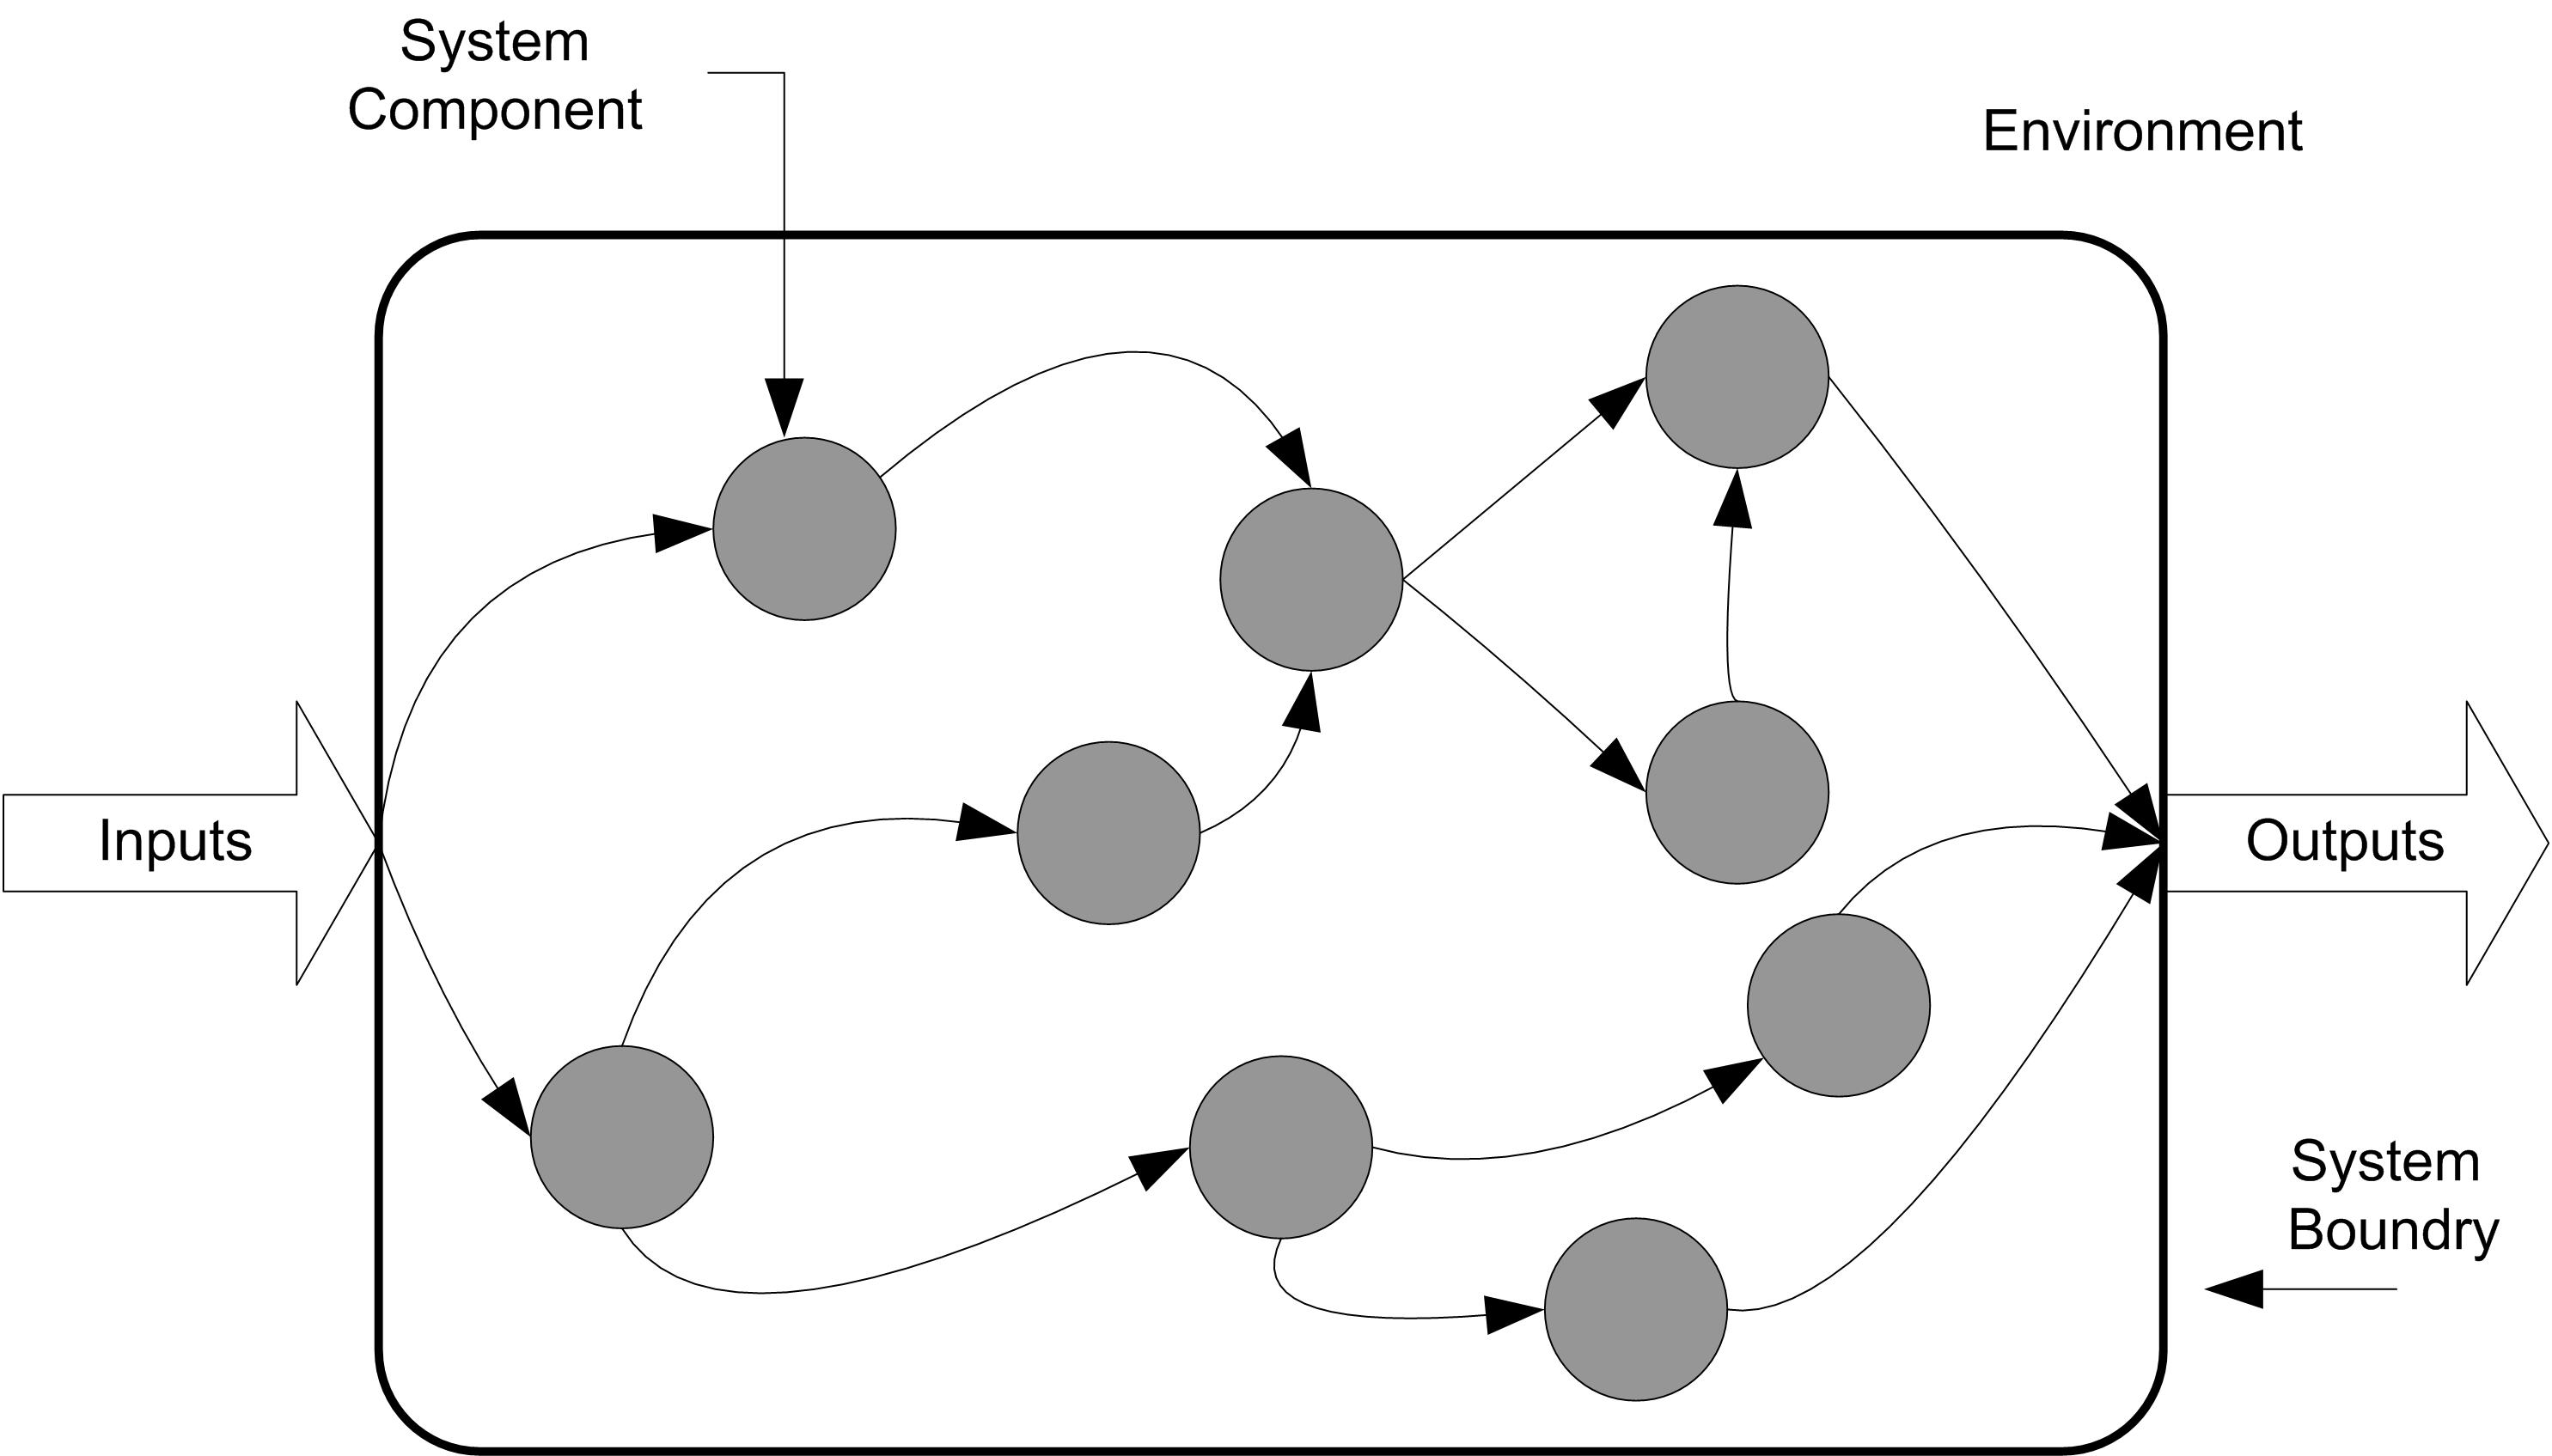
\includegraphics{./figures2/ch1/ch1fig1} 

}

\caption{Conceptualization of a System}\label{fig:ch1SystemConcept}
\end{figure}

Because how you conceptualize a system drives your modeling, it is
useful to discuss some general system classifications. Systems might be
classified by whether or not they are man-made (e.g.~manufacturing
system) or whether they are natural (e.g.~solar system). A system can be
physical (e.g.~an airport) or conceptual (e.g.~a system of equations).
If stochastic or random behavior is an important component of the system
then the system is said to be stochastic, if not then it is considered
deterministic. One of the more useful ways to look at a system is
whether it changes with respect to time. If a system does not change
significantly with respect to time it is said to be static, else it is
called dynamic. If a system is dynamic, you might want to consider how
it evolves with respect to time. A dynamic system is said to be discrete
if the state of the system changes at discrete points in time. A dynamic
system is said to be continuous if the state of the system changes
continuously with time. This dichotomy is purely a function of your
level of abstraction. If conceptualizing a system as discrete, serves
our purposes then you can call the system discrete.
Figure \ref{fig:ch1SystemTypes} illustrates this classification of
systems. This book primarily examines stochastic, dynamic, discrete
systems.

\begin{figure}

{\centering 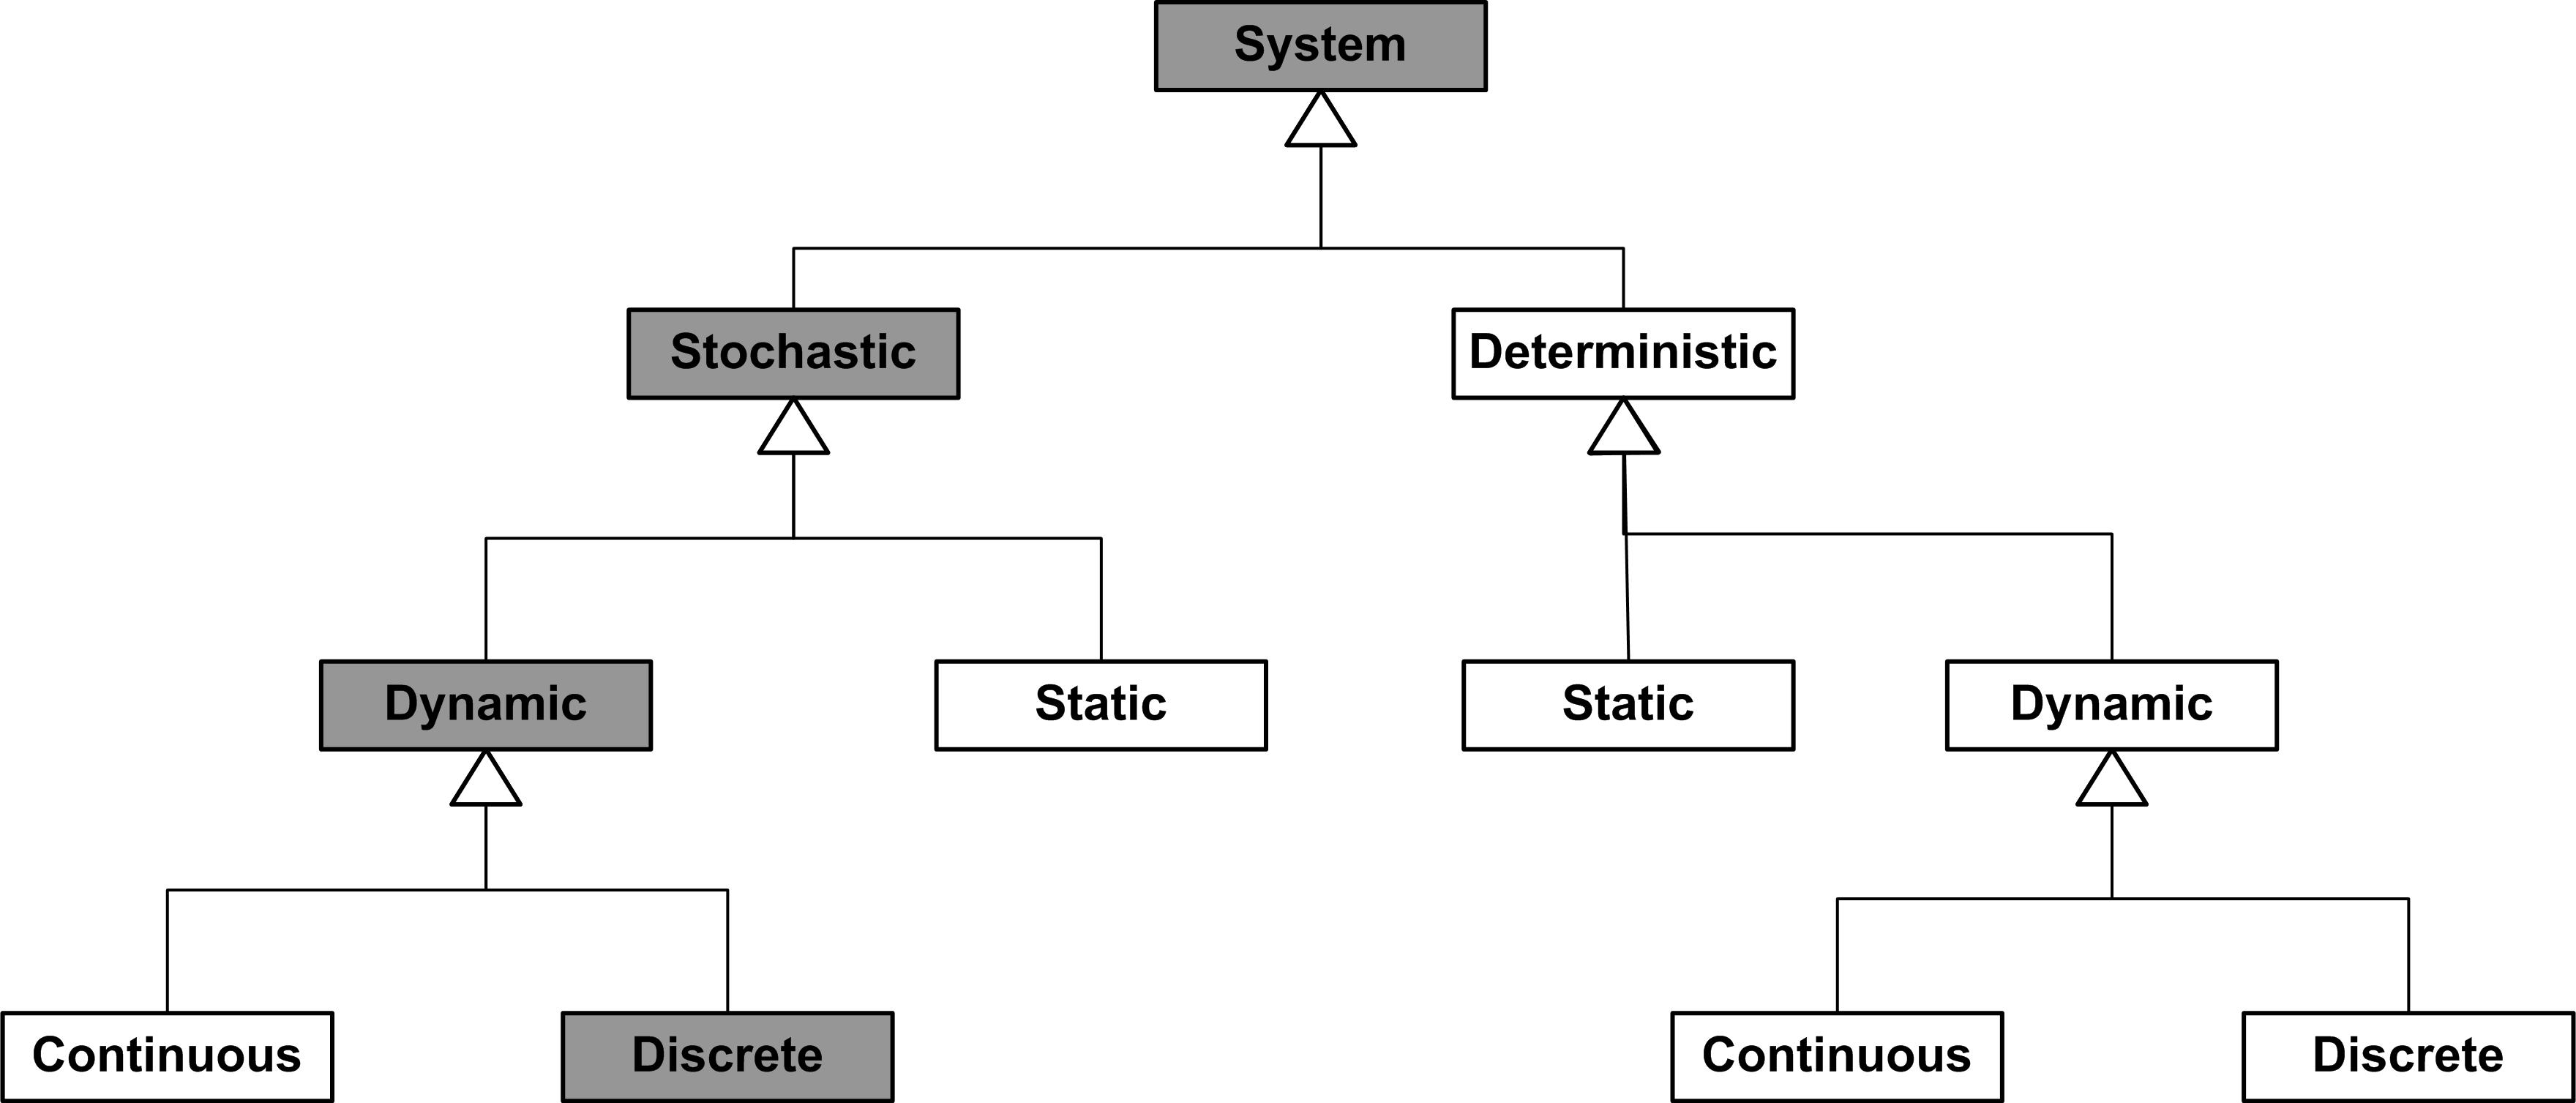
\includegraphics{./figures2/ch1/ch1fig2} 

}

\caption{General Types of Systems}\label{fig:ch1SystemTypes}
\end{figure}

The main purpose of a simulation model is to allow observations about a
particular system to be gathered as a function of time. From that
standpoint, there are two distinct types of simulation: 1) discrete
event and 2) continuous.

Just as discrete systems change at discrete points in time, in discrete
event simulation observations are gathered at selected points in time
when certain changes take place in the system. These selected points in
time are called events. On the other hand, continuous simulation
requires that observations be collected continuously at every point in
time (or at least that the system is described for all points in time).
The types of models to be examined in this book are called
discrete-event simulation models.

To illustrate the difference between the two types of simulation,
contrast a fast food service counter with that of oil loading facility
that is filling tankers. In the fast food service counter system,
changes in the status of the system occur when a customer either arrives
to place an order or when the customer receives their food. At these two
events, measures such as queue length and waiting time will be affected.
At all the other points in time, these measures remain either unchanged
(e.g.~queue length) or not yet ready for observation (e.g.~waiting time
of the customer). For this reason, the system does not need to be
observed on a continuous basis. The system need only be observed at
selected discrete points in time, resulting in the applicability of a
discrete-event simulation model.

In the case of the oil tanker loading example, one of the measures of
performance is the amount of oil in each tanker. Because the oil is a
liquid, it cannot be readily divided into discrete components. That is,
it flows continuously into the tanker. It is not necessary (or
practical) to track each molecule of oil individually, when you only
care about the level of the oil in the tanker. In this case, a model of
the system must describe the rate of flow over time and the output of
the model is presented as a function of time. Systems such as these are
often modeled using differential equations. The solution of these
equations involves numerical methods that integrate the state of the
modeled system over time. This, in essence, involves dividing time into
small equal intervals and stepping through time.

Often both the discrete and continuous viewpoints are relevant in
modeling a system. For example, if oil tanker arrives at the port to be
filled, we have an arrival event that changes the state of the system.
This type of modeling situation is called combined continuous discrete
modeling.

A system and our resulting model depends on how we characterize the state of the system. The \textbf{state} of a system is the set of properties/variables that
describe the system at any time \(\{x_1(t), x_2(t), \dots\}\) where \(x_1(t)\) is a
variable that represents a system property value at time \(t\). Variables that take
on a countable set of values are \textbf{discrete}. Variables that take on an
uncountable set of values are said to be \textbf{continuous}. For discrete
variables, we can define a mapping from the set of integers to each
possible value. Even in the discrete case, there may be an infinite number of values. Continuous
variables are represented by the set of real numbers. That is, there are
an uncountably infinite number of possible values that the variable can take on.

A discrete system has all discrete variables in its state. A continuous
system has all continuous variables in its state. A combined
continuous-discrete system has both types of variables in defining its
state. Consider an airplane:

\begin{itemize}
\item
  If we are interested in the number of parts operating to
  specification at any time t, then the state is \(\{N_1(t), N_2(t), \dots \}\)
  where \(N_1(t) = 1\) if part 1 is operating and 0 if part 1 is not
  operating to specification. The state vector consists of all
  discrete variables. This is a discrete system.
\item
  If we are interested in the temperature of each part at time \(t\), then
  the state is \(\{T_1(t), T_2(t), \dots \}\), where \(T_1(t)\) is the temperature
  in Celsius of part 1 at time \(t\), etc. The state vector consists of
  all continuous variables. This is continuous system.
\item
  If we are interested in the velocity of a plane at time \(t\) and the
  number of wheels deployed at time \(t\), then the state is \(\{v(t), n(t)\}\)
  where \(v(t)\) is the velocity of the plane in meters/second and \(n(t)\) is
  \(\{0,1,2,3,4\}\) wheels. Then the state vector consists of both
  continuous and discrete variables that change with time. This is a
  combined continuous/discrete system.
\end{itemize}

Static systems are systems for which time is not a significant factor. In other words, that the
state does not evolve over time. Dynamic systems are systems for which
system state changes with respect to time. In a deterministic system, the variables
are not governed by underlying random processes. In a stochastic
system, some of the variables are governed by underlying random
processes. Time can change continuously or at discrete points. When time
changes only at discrete points in time, we call these points, events.

Some simulation languages have modeling constructs for both
continuous and discrete modeling; however, this book does not cover the
modeling of continuous or combined continuous discrete systems. There are
many useful references on this topic. We will be modeling discrete-event dynamic stochastic systems in this textbook.

\hypertarget{simulation-descriptive-or-prescriptive-modeling}{%
\section{Simulation: Descriptive or Prescriptive Modeling?}\label{simulation-descriptive-or-prescriptive-modeling}}

A descriptive model describes how a system behaves. Simulation is at its
heart a descriptive modeling technique. Simulation is used to depict the
behaviors or characteristics of existing or proposed systems. However, a
key use of simulation is to convey the \emph{required} behaviors or
properties of a proposed system. In this situation, simulation is used
to prescribe a solution. A prescriptive model tells us what to do. In
other words, simulation can also be used for prescriptive modeling.
Figure \ref{fig:ch1PrescriptiveSimulation} illustrates the concept of
using simulation to recommend a solution.

\begin{figure}

{\centering 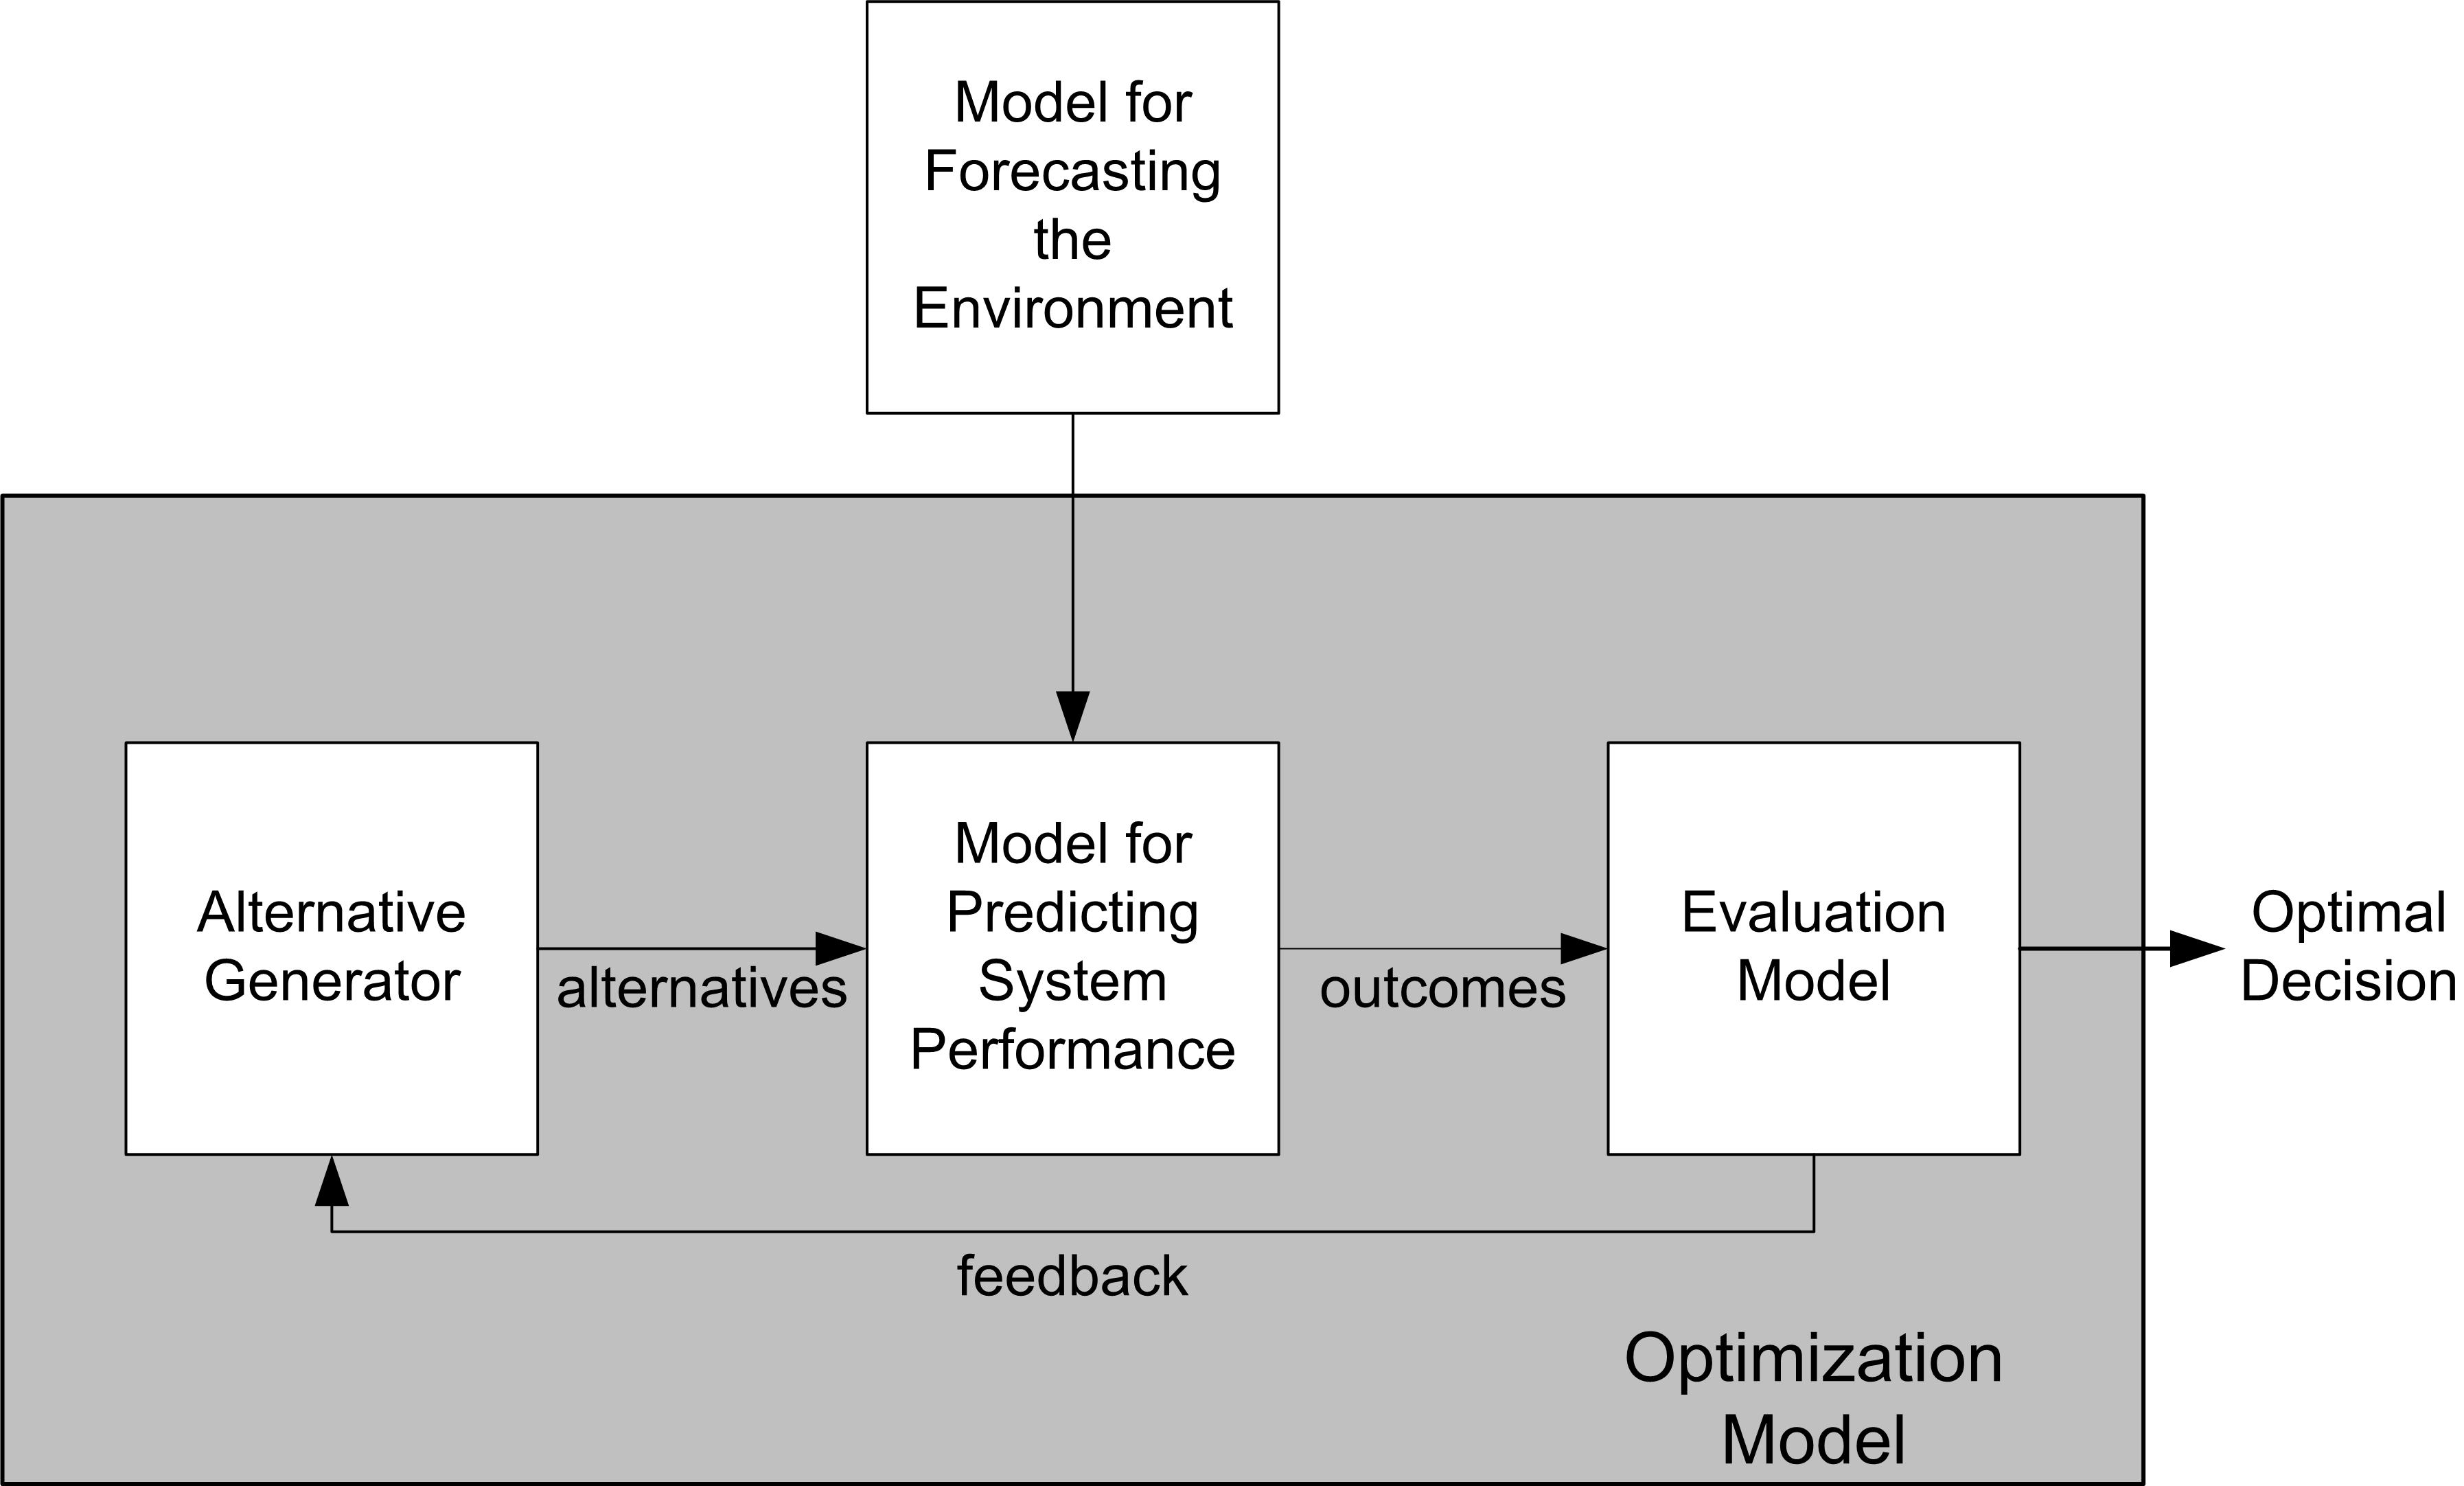
\includegraphics{./figures2/ch1/ch1fig3} 

}

\caption{Using Simulation for Prescriptive Analysis}\label{fig:ch1PrescriptiveSimulation}
\end{figure}

In the figure, a simulation model is used for predicting the behavior of
the system. Input models are used to characterize the system and its
environment. An evaluative model is used to evaluate the output of the
simulation model to understand how the output compares to desired goals.
The alternative generator is used to generate different scenarios to be
feed into the simulation model for evaluation. Through a feedback
mechanism the inputs can be changed based on the evaluation of the
outputs and eventually a recommended solution can be achieved.

For example, in the modeling a drive up pharmacy, suppose that the
probability of a customer waiting longer than 3 minutes in line had to
be less than 10\%. To form design alternatives, the inputs (e.g.~number
of pharmacists, possibly the service process) can be varied. Each
alternative can then be evaluated to see if the waiting time criteria is
met. In this simple situation, you might act as your own alternative
generator and the evaluative model is as simple as meeting a criteria;
however, in more complex models, there will often be hundreds of inputs
to vary and multiple competing objectives. In such situations,
simulation optimization and heuristic search methods are often used.
This is an active and important area of research within simulation.

\hypertarget{randomness-in-simulation}{%
\section{Randomness in Simulation}\label{randomness-in-simulation}}

In most real-life situations, the arrival process and the service
process occur in a random fashion. Even though the processes may be
random, it does not mean that you cannot describe or model the
randomness. To have any hope of simulating the situation, you must be
able to model the randomness. One of the ways to model this randomness
is to describe the phenomenon as a random variable governed by a
particular probability distribution. For example, if the arrivals to the
bank occur according to a Poisson process, then from probability theory
it is known that the distribution of inter-arrival times is an
exponential distribution. In general, information about how the
customers arrive must be secured either through direct observation of
the system or by using historical data. If neither source of information
is available, then some plausible assumptions must be made to describe
the random process by a probability model.

If historical data is available, there are two basic choices for how to
handle the modeling. The first choice is to develop a probability model
given the data. The second choice is to try to drive the simulation
directly from the historical data. The latter approach is not
recommended. First of all, it is extremely unlikely that the captured
data will be in a directly usable form. Secondly, it is even more
unlikely that the data will be able to adequately represent all the
modeling scenarios that you will need through the course of
experimenting with the model. For example, suppose that you only have 1
day's worth of arrival data, but you need to simulate a month's worth of
system operation. If you simply re-drive your simulation using the 1
day's worth of data, you are not simulating different days! It is much
more advisable to develop probability models either from historical data
or from data that you capture in developing your model. Appendix \ref{app:idm}
discusses some of the tools and techniques for modeling probability
distributions.

Once a probability model has been developed, statistical theory provides
the means for obtaining random samples based on the use of uniformly
distributed random numbers on the interval (0,1). These random samples
are then used to map the future occurrence of an event on the time
scale. For example, if the inter-arrival time is exponential then a
random sample drawn from that distribution would represent the time
interval until the occurrence of the next arrival. The process of
generating random numbers and random variables within simulation is
presented in Appendix \ref{app:rnrv}.

\hypertarget{simulation-languages}{%
\section{Simulation Languages}\label{simulation-languages}}

Discrete event simulation normally involves a tremendous volume of
computation. Consequently, the use of computers to carry out these
computations is essential; however, the volume of computations is not
the only obstacle in simulation. If you consider the bank teller example
discussed in the previous sections, you will discover that it involves a
complex logical structure that requires special expertise before it can
be translated into a computer model. Attempting to implement the
simulation model, from scratch, in a general purpose language such as
FORTRAN, Visual Basic, C/C++, or Java will require above average
programming skills. In the absence of specialized libraries for these
languages that try to relive the user from some of the burden,
simulation as a tool would be relegated to "elite" programmers.
Luckily, the repetitive nature of computations in simulation allows the
development of computer libraries that are applicable to simulation
modeling situations. For example, libraries or packages must be
available for ordering and processing events chronologically, as well as
generating random numbers and automatically collecting statistics. Such
a library for simulating discrete-event systems in Java is available
from the author, see \citep{Rossetti2008aa}.

The computational power and storage capacity of computers has motivated
the development of specialized simulation languages. Some languages have
been developed for continuous or discrete simulations. Others can be
used for combined continuous and discrete modeling. All simulation
languages provide certain standard programming facilities and will
differ in how the user will take advantage of these facilities. There is
normally some trade-off between how flexible the language is in
representing certain modeling situations. Usually, languages that are
highly flexible in representing complex situations require more work
(and care) by the user to account for how the model logic is developed.
Some languages are more programming oriented (e.g.~SIMSCRIPT) and others
are more "drag and drop" (e.g.~ProModel, Arena, etc. ).

The choice of a simulation language is a difficult one. There are many
competing languages, each having their own advantages and disadvantages.
The Institute for Operations Research and Management Science (INFORMS)
often has a yearly product review covering commercial simulation
languages, see for example (\url{http://lionhrtpub.com/orms/}). In addition to
this useful comparison, you should examine the Winter Simulation
Conference (www.wintersim.org). The conference has hands on exhibits of
simulation software and the conference proceedings often have tutorials
for the various software packages. Past proceedings have been made
available electronically through the generous support of the INFORMS
Society for Simulation (\url{http://www.informs-sim.org/wscpapers.html}).

was chosen for this textbook because of the author's experience
utilizing the software, its ease of use, and the availability of student
versions of the software. While all languages have flaws, using a
simulation language is essential in performing high performance
simulation studies. Most, if not all simulation companies have strong
support to assist the user in learning their software. has a strong
academic and industrial user base and is very competitive in the
simulation marketplace. Once you learn one simulation language well, it
is much easier to switch to other languages and to understand which
languages will be more appropriate for certain modeling situations.

is fundamentally a process description based language. That is, when
using , the modeler describes the process that an "entity" experiences
while flowing through or using the elements of the system. You will
learn about how facilitates process modeling throughout this textbook.

\hypertarget{ch1:sec:simMeth}{%
\section{Simulation Methodology}\label{ch1:sec:simMeth}}

This section presents a brief overview of the steps of simulation
modeling by discussing the process in the context of a methodology. A
methodology is simply a series of steps to follow. Since simulation
involves systems modeling, a simulation methodology based on the general
precepts of solving a problem through systems analysis is presented
here. A general methodology for solving problems can be stated as
follows:

\begin{enumerate}
\def\labelenumi{\arabic{enumi}.}
\item
  Define the problem
\item
  Establish measures of performance for evaluation
\item
  Generate alternative solutions
\item
  Rank alternative solutions
\item
  Evaluate and Iterate during process
\item
  Execute and evaluate the solution
\end{enumerate}

This methodology can be referred to by using the first letter of each
step. The DEGREE methodology for problem solving represents a series of
steps that can be used during the problem solving process. The first
step helps to ensure that you are solving the right problem. The second
step helps to ensure that you are solving the problem for the right
reason, i.e.~your metrics must be coherent with your problem. Steps 3
and 4 ensure that the analyst looks at and evaluates multiple solutions
to the problem. In other words, these steps help to ensure that you
develop the right solution to the problem. A good methodology recognizes
that the analyst needs to evaluate how well the methodology is doing. In
step 5, the analyst evaluates how the process is proceeding and allows
for iteration. Iteration is an important concept that is foreign to many
modelers. The concept of iteration recognizes that the problem solving
process can be repeated until the desired degree of modeling fidelity
has been achieved. Start the modeling at a level that allows it to be
initiated and do not try to address the entire situation in each of the
steps. Start with small models that work and build them up until you
have reached your desired goals. It is important to get started and get
something established on each step and continually go back in order to
ensure that the model is representing reality in the way that you
intended. The final step is often over looked. Simulation is often used
to recommend a solution to a problem. Step 6 indicates that if you have
the opportunity you should execute the solution by implementing the
decisions. Finally, you should always follow up to ensure that the
projected benefits of the solution were obtained.

The DEGREE problem solving methodology should serve you well; however,
simulation involves certain unique actions that must be performed during
the general overall problem solving process. When applying DEGREE to a
problem that may require simulation, the general DEGREE approach needs
to be modified to explicitly consider how simulation will interact with
the overall problem solving process.

Figure \ref{fig:ch1SimMethodology} represents a refined general
methodology for applying simulation to problem solving.

\begin{enumerate}
\def\labelenumi{\arabic{enumi}.}
\item
  Problem Formulation

  \begin{enumerate}
  \def\labelenumii{\arabic{enumii}.}
  \item
    Define the problem
  \item
    Define the system
  \item
    Establish performance metrics
  \item
    Build conceptual model
  \item
    Document model assumptions
  \end{enumerate}
\item
  Simulation Model Building

  \begin{enumerate}
  \def\labelenumii{\arabic{enumii}.}
  \item
    Model translation
  \item
    Input data modeling
  \item
    Verification
  \item
    Validation
  \end{enumerate}
\item
  Experimental Design and Analysis

  \begin{enumerate}
  \def\labelenumii{\arabic{enumii}.}
  \item
    Preliminary Runs
  \item
    Final experiments
  \item
    Analysis of results
  \end{enumerate}
\item
  Evaluate and Iterate

  \begin{enumerate}
  \def\labelenumii{\arabic{enumii}.}
  \item
    Documentation
  \item
    Model manual
  \item
    User manual
  \end{enumerate}
\item
  Implementation
\end{enumerate}

The first phase, problem formulation, captures the essence of the first
two steps in the DEGREE process. The second phase, model building,
captures the essence of step 3 of the DEGREE process. When building
models, you are either explicitly or implicitly developing certain
design alternatives. The third phase, experimental design and analysis,
encapsulates some of steps 3 and 4 of the DEGREE process. In designing
experiments, design alternatives are specified and when analyzing
experiments their worth is being evaluated with respect to problem
objectives. The fourth phase, evaluate and iterate, captures the notion
of iteration. Finally, the fifth and sixth phases, documentation and
implementation complete the simulation process. Documentation is
essential when trying to ensure the ongoing and future use of the
simulation model, and implementation recognizes that simulation projects
often fail if there is no follow through on the recommended solutions.

\begin{figure}

{\centering 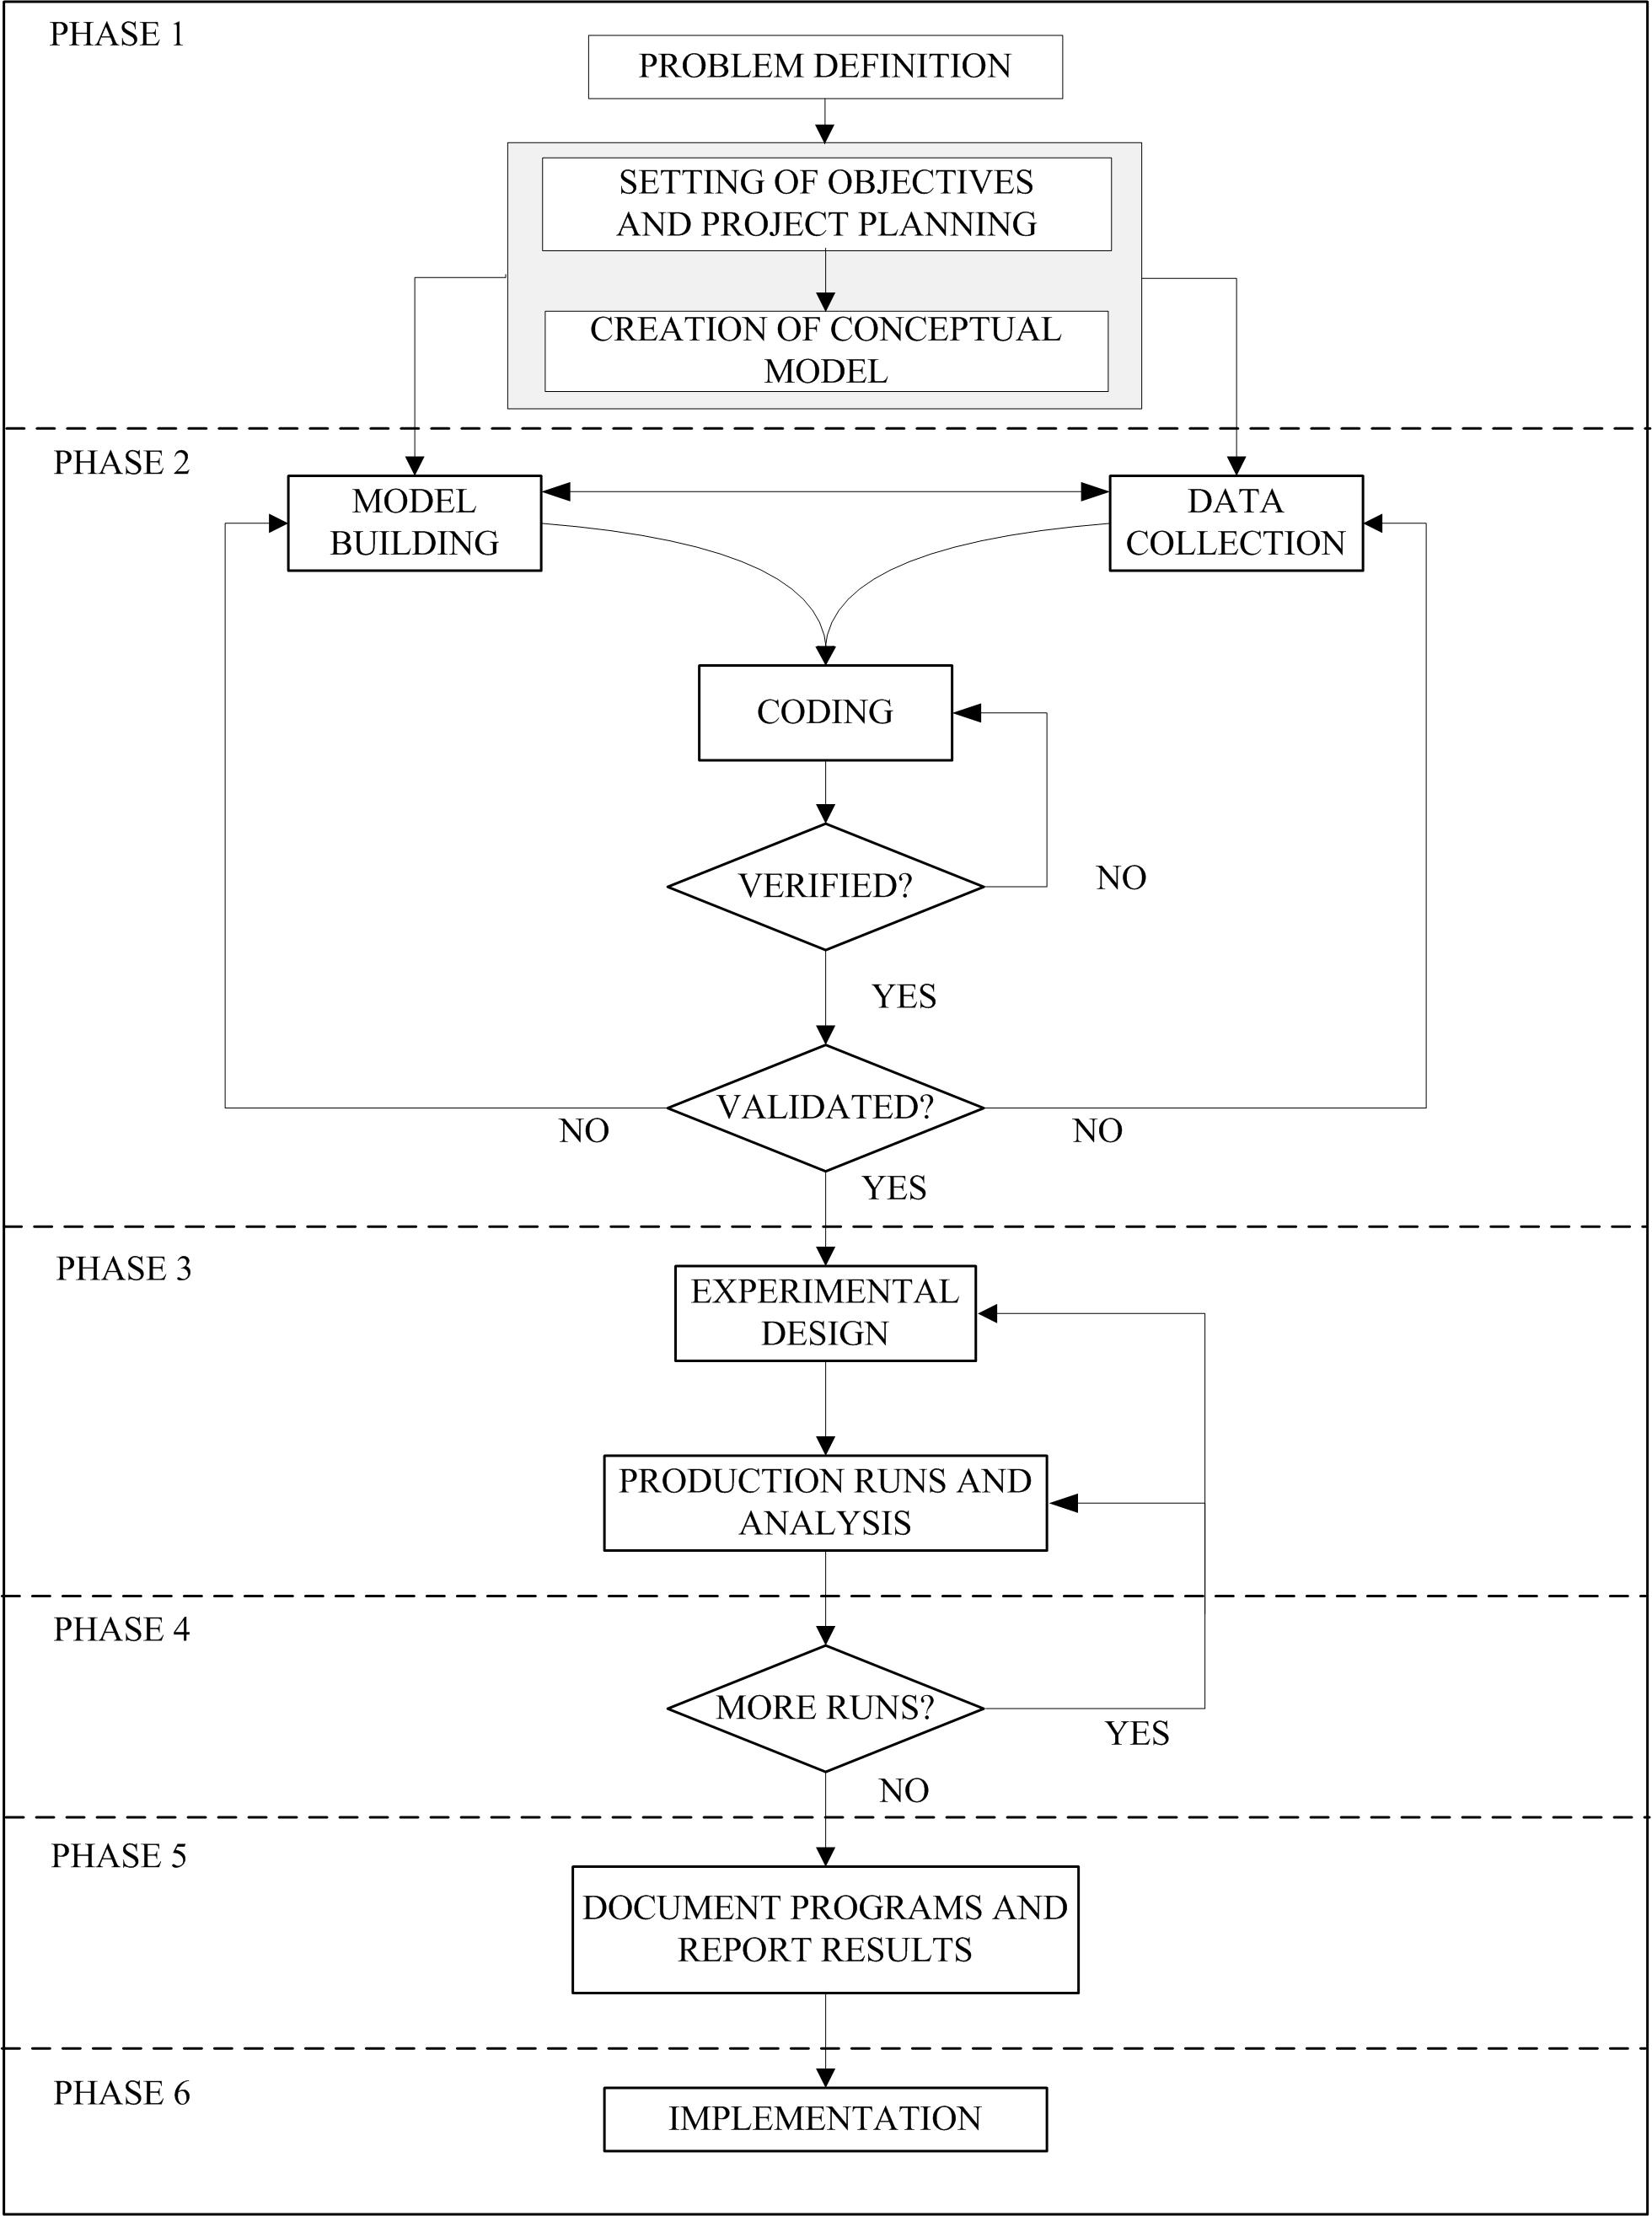
\includegraphics{./figures2/ch1/ch1fig4} 

}

\caption{General Simulation Methodology}\label{fig:ch1SimMethodology}
\end{figure}

The problem formulation phase of the study consists of five primary
activities:

\begin{enumerate}
\def\labelenumi{\arabic{enumi}.}
\item
  Defining the problem
\item
  Defining the system
\item
  Establishing performance metrics.
\item
  Building conceptual models
\item
  Documenting modeling assumptions
\end{enumerate}

A problem starts with a perceived need. These activities are useful in
developing an appreciation for and an understanding of what needs to be
solved. The basic output of the problem definition activity is a problem
definition statement. A problem definition statement is a narrative
discussion of the problem. A problem definition statement is necessary
to accurately and concisely represent the problem for the analyst and
for the problem stakeholders. This should include all the required
assumptions made during the modeling process. It is important to
document your assumptions so that you can examine their effect on the
model during the verification, validation, and experimental analysis
steps of the methodology. This ensures that the problem is well
understood and that all parties agree upon the nature of the problem and
the goals of the study. The general goals of a simulation study often
include:

\begin{itemize}
\item
  Comparison: To compare system alternatives and their performance
  measures across various factors (decision variables) with respect to
  some objectives
\item
  Optimization: This is a special case of comparison in which you try
  to find the system configuration that optimizes performance subject
  to constraints.
\item
  Prediction: To predict the behavior of the system at some future
  point in time.
\item
  Investigation: To learn about and gain insight into the behavior of
  the system given various inputs.
\end{itemize}

These general goals will need to be specialized to the problem under
study. The problem definition should include a detailed description of
the objectives of the study, the desired outputs from the model, and the
types of scenarios to be examined or decisions to be made.

The second activity of this phase produces a definition of the system. A
system definition statement is necessary to accurately and concisely
define the system, particularly its boundaries. The system definition
statement is a narrative, which often contains a pictorial
representation of the major elements of the system. This ensures that
the simulation study is focused on the appropriate areas of interest to
the stakeholders and that the scope of the project is well understood.

When defining the problem and the system, one should naturally begin to
develop an understanding of how to measure system performance. The third
activity of problem formulation makes this explicit by encouraging the
analyst to define the required performance measures for the model. To
meaningfully compare alternative scenarios, objective and measurable
metrics describing the performance of the system are necessary. The
performance metrics should include quantitative statistical measures
from any models used in the analysis (e.g.~simulation models),
quantitative measures from the systems analysis, (e.g.~cost/benefits),
and qualitative assessments (e.g.~technical feasibility, human,
operational feasibility). The focus should be placed on the performance
measures that are considered to be the most important to system
decision-makers and tied directly to the objectives of the simulation
study. Evaluation of alternatives can then proceed in an objective and
unbiased manner to determine which system scenario performs the best
according to the decision maker's preferences.

The problem definition statement, the system definition statement, and
explicit performance metrics set the stage for more detailed modeling.
These activities should be captured in a written form. Within this text,
you will develop models of certain ``ready-made'' book problems. One way
to accomplish the problem formulation phase of a simulation study is to
consider writing yourself a "book problem". You will need enough
detail in these documents that a simulation analyst (you) can develop a
model in any simulation language for the given situation.

With a good understanding of the problem and of the system under study,
you should be ready to begin your detailed model formulations. Model
formulation does not mean a computer program. You should instead use
conceptual modeling tools: conceptual diagrams, flow charts, etc. prior
to any use of software to implement a model. The purpose of conceptual
modeling tools is to convey a more detailed system description so that
the model may be translated into a computer representation. General
descriptions help to highlight the areas and processes of the system
that the model will simulate. Detailed descriptions assist in simulation
model development and coding efforts. Some relevant diagramming
constructs include:

\begin{enumerate}
\def\labelenumi{\arabic{enumi}.}
\item
  Context Diagrams: A context diagram assists in conveying the general
  system description. The diagram is a pictorial representation of the
  system that often includes flow patterns typically encountered.
  Context diagrams are often part of the system description document.
  There are no rules for developing context diagrams. If you have an
  artistic side, here is your opportunity to shine!
\item
  Activity Diagrams: An activity diagram is a pictorial representation
  of the process for an entity and its interaction with resources
  while within the system. If the entity is a temporary entity (i.e.
  it flows through the system) the activity diagram is called an
  activity flow diagram. If the entity is permanent (i.e.~it remains
  in the system throughout its life) the activity diagram is called an
  activity cycle diagram. Activity diagrams will be used extensively
  within this text.
\item
  Software engineering diagrams: Because simulation entails software
  development, the wide-variety of software engineering diagramming
  techniques can be utilized to provide information for the model
  builder. Diagrams such as flow charts, database diagrams, IDEF (ICAM
  DEFinition language) diagrams, UML (unified modeling language)
  diagrams, state charts, etc are all useful in documenting complex
  modeling situations. These techniques assist development and coding
  efforts by focusing attention on describing, and thus understanding,
  the elements within the system. Within this text, activity diagrams
  will be augmented with some simple flow chart symbols and some
  simple state diagrams will be used to illustrate a variety of
  concepts.
\end{enumerate}

In your modeling, you should start with an easy conceptual model that
captures the basic aspects and behaviors of the system. Then, you should
begin to add details, considering additional functionality. Finally, you
should always remember that the complexity of the model has to remain
proportional to the quality of the available data and the degree of
validity necessary to meet the objectives of the study. In other words,
don't try to model the world!

After developing a solid conceptual model of the situation, simulation
model building can begin. During the simulation model building phase,
alternative system design configurations are developed based on the
previously developed conceptual models. Additional project planning is
also performed to yield specifications for the equipment, resources, and
timing required for the development of the simulation models. The
simulation models used to evaluate the alternative solutions are then
developed, verified, validated, and prepared for analysis. Within the
context of a simulation project this process includes:

\begin{itemize}
\item
  Input Data Preparation: Input data is analyzed to determine the
  nature of the data and to determine further data collection needs.
  Necessary data is also classified into several areas. This
  classification establishes different aspects of the model that are
  used in model development.
\item
  Model Translation: Description of the procedure for coding the
  model, including timing and general procedures and the translation
  of the conceptual models into computer simulation program
  representations.
\item
  Verification: Verification of the computer simulation model is
  performed to determine whether or not the program performs as
  intended. To perform model verification, model debugging is
  performed to locate any errors in the simulation code. Errors of
  particular importance include improper flow control or entity
  creation, failure to release resources, and logical/arithmetic
  errors or incorrectly observed statistics. Model debugging also
  includes scenario repetition utilizing identical random number
  seeds, "stressing" the model through a sensitivity analysis
  (varying factors and their levels) to ensure compliance with
  anticipated behavior, and testing of individual modules within the
  simulation code.
\item
  Validation: Validation of the simulation model is performed to
  determine whether or not the simulation model adequately represents
  the real system. The simulation model is shown to personnel (of
  various levels) associated with the system in question. Their input
  concerning the realism of the model is critical in establishing the
  validity of the simulation. In addition, further observations of the
  system are performed to ensure model validity with respect to actual
  system performance. A simple technique is to statistically compare
  the output of the simulation model to the output from the real
  system and to analyze whether there is a significant (and practical)
  difference between the two.
\end{itemize}

Model translation will be a large component of each chapter as you learn
how to develop simulation models. Verification and validation techniques
will not be a major component of this text, primarily because the models
will be examples made for educational purposes. This does not mean that
you should ignore this important topic. You are encouraged to examine
many of the useful references on validation, see for example
\citep{balci1997principles} and \citep{balci1998verification}.

After you are confident that your model has been verified and validated
to suit your purposes, you can begin to use the model to perform
experiments that investigate the goals and objectives of the project.
Preliminary simulation experiments should be performed to set the
statistical parameters associated with the main experimental study. The
experimental method should use the simulation model to generate
benchmark statistics of current system operations. The simulation model
is then altered to conform to a potential scenario and is re-run to
generate comparative statistics. This process is continued, cycling
through suggested scenarios and generating comparative statistics to
allow evaluation of alternative solutions. In this manner, objective
assessments of alternative scenarios can be made.

For a small set of alternatives, this ``one at a time'' approach is
reasonable; however, often there are a significant number of design
factors that can affect the performance of the model. In this situation,
the analyst should consider utilizing formal experimental design
techniques. This step should include a detailed specification of the
experimental design (e.g.~factorial, etc) and any advanced output
analysis techniques (e.g.~batching, initialization bias prevention,
variance reduction techniques, multiple comparison procedures, etc.)
that may be required during the execution of the experiments. During
this step of the process, any quantitative models developed during the
previous steps are exercised. Within the context of a simulation
project, the computer simulation model is exercised at each of the
design points within the stipulated experimental design.

Utilizing the criteria specified by system decision-makers, and
utilizing the simulation model's statistical results, alternative
scenarios should then be analyzed and ranked. A methodology should be
used to allow the comparison of the scenarios that have multiple
performance measures that trade-off against each other.

If you are satisfied that the simulation has achieved your objectives
then you should document and implement the recommended solutions. If
not, you can iterate as necessary and determine if any additional data,
models, experimentation, or analysis is needed to achieve your modeling
objectives. Good documentation should consist of at least two parts: a
technical manual, which can be used by the same analyst or by other
analysts, and a user manual. A good technical manual is very useful when
the project has to be modified, and it can be a very important
contribution to software reusability and portability. The approach to
documenting the example models in this text can be used as an example
for how to document your models. In addition to good model development
documentation, often the simulation model will be used by non-analysts.
In this situation, a good user manual for how to use and exercise the
model is imperative. The user manual is a product for the user who may
not be an expert in programming or simulation issues; therefore
clearness and simplicity should be its main characteristics. If within
the scope of the project, the analyst should also develop implementation
plans and follow through with the installation and integration of the
proposed solutions. After implementation, the project should be
evaluated as to whether or not the proposed solution met the intended
objectives.

In this textbook, we will use an open source library for performing stochastic discrete event simulation called the Java Simulation Library (JSL). The next section provides a brief overview.

\hypertarget{overview-of-the-java-simulation-library}{%
\section{Overview of the Java Simulation Library}\label{overview-of-the-java-simulation-library}}

The JSL (a Java Simulation Library) is a simulation library for Java. The JSL's current version has packages that support random number generation, statistical collection, basic reporting, and discrete-event simulation modeling.

The purpose of the JSL is to support education and research within simulation. Current simulation languages hide the implementation details of the workings of a simulation. As such, students exposed to a simulation language such as (ProModel, Arena, and AutoMod, etc.) are able to learn the practice of simulation without having a detailed understanding of the fundamental mechanisms that enable the technology. This has both advantages and disadvantages. The advantage is that more engineers are capable of using and applying simulation technology to improve systems. The disadvantage is that their modeling abilities depend heavily on a particular software package and simulation modeling has the potential to become a black-box technology. I've seen many users who can build complicated models, but have limited or no understanding of how the simulation actually works.

When teaching simulation, especially at the undergraduate level, simulation languages enable students with introductory programming skills to model systems and perform experiments. Within a typical introductory semester course on simulation it is possible to cover the basics of simulation (random numbers, modeling, and statistical analysis) along with the coverage of a tool (Arena, ProModel, AutoMod, etc.) It is difficult to teach students how simulation works based on a general purpose programming language due to the reduced emphasis on more advanced programming skills especially for non-computer science majors. The JSL assists in bridging this gap by providing a standard library in Java for simulation modeling. One of the fundamental design goals of the JSL is to clearly demonstrate how one can implement the fundamental mechanisms that enable simulation technology. By studying the implementation details students will gain a deeper understanding of how simulation works. They will become better simulation modelers, practitioners, and users of commercial simulation languages.

The JSL also supports research within simulation. Naturally, the JSL can be used as a modeling tool to simulate complex systems. Simulators, such as a Supply Chain Simulator, can be built based on the JSL framework. In addition, the design of the JSL provides a framework for the testing of simulation artifacts through a well-defined class and interface hierarchy. The structure of the JSL permits the easy switching of various components within a simulation, the event calendar, random number generator, statistics, etc. For example, the efficiency of different event calendars can be easily tested by simply providing an event calendar to the JSL that implements the interface CalendarIfc. Different algorithms can be ``plugged into'' the framework for testing.

This document presents an overview of a simulation library for Java (JSL). The library is divided into Java packages (calendar, examples, exceptions, modeling, observers, testing, and utilities). As necessary, these packages may contain sub-packages, which implement various aspects of the library. The JSL is organized as three open source projects: JSLCore, JSLExamples, and JSLExtensions. Each of these projects is further organized into java packages.

JSLCore - jsl is the main package that holds all sub-packages

\begin{itemize}
\tightlist
\item
  calendar - The calendar package implements classes that provide event calendar processing
\item
  simulation - The simulation package implements the main classes involved in constructing and running simulation.
\item
  modeling - The modeling package is the heart of the JSL. In the modeling package, supporting model elements such as queues, resources, variables, commands, etc. are implemented. This package will be discussed in detail in this document.

  \begin{itemize}
  \tightlist
  \item
    observers - The observers package provides support classes for observing model elements during the simulation run. The JSL is designed to allow each model element to have observers attached to it thereby implementing the classic Observer pattern. Observers can be used to collect statistics, write output to files, display model element state, etc. Proper understanding of the observer pattern is essential in maximizing the use of the JSL.
  \item
    utilities - The utilities package provides support classes that are used by the JSL. The random, statistics, reporting, and database related sub-packages will be discussed in this document.
  \end{itemize}
\end{itemize}

JSLExtensions - jslx is the main package that holds all sub-packages

\begin{itemize}
\tightlist
\item
  dbutilities - The dbutilities package provides support for using databases with the JSL. It also includes some functionality related to csv and Excel files
\item
  fxutilities - The fxutilities provides some simple support for javaFx
\item
  statistics - The statistics package provide additional statistical functionality that leverages the additional classes available within the jslx package.
\end{itemize}

JSLExamples - examples is the main package that holds all sub-packages

\begin{itemize}
\tightlist
\item
  entity - examples related to modeling entity flow and process description
\item
  hospitalward - an example of modeling a hospital ward
\item
  inventoy - some simple inventory policy models
\item
  jobshop - models the classic job shop example from Law and Kelton's textbook
\item
  jockeying - models queues with jockeying of customers
\item
  modelelement - examples related to the use of model elements
\item
  models - many example models
\item
  montecarlo - examples focused on using random numbers and Monte Carlo methods
\item
  queueing - examples related to systems involving queues
\item
  resource - examples that illustrate resource constructs
\item
  spatial - examples related to the spatial package in JSLCore
\item
  station - examples illustrating the station package in JSLCore
\item
  utilities - miscellaneous examples of using constructs in the utilities
\item
  variables - examples of using variables within models
\end{itemize}

The purpose of the JSL is to provide support for the development of discrete-event simulation programs within Java. This document provides and overview of the functionality and use of the classes found within the JSL. Additional information is available through the JavaDoc API. We begin our discussion with the utilities package within the JSLCore. These support packages can be used independently of building discrete-event simulation models.

\hypertarget{exercises}{%
\section{Exercises}\label{exercises}}

\begin{center}\rule{0.5\linewidth}{0.5pt}\end{center}

\begin{exercise}
\protect\hypertarget{exr:ch1P1}{}{\label{exr:ch1P1} }Using the resources at
(\url{http://www.informs-sim.org/wscpapers.html}) find an application of
simulation to a real system and discuss why simulation was important to
the analysis.
\end{exercise}

\begin{center}\rule{0.5\linewidth}{0.5pt}\end{center}

\begin{exercise}
\protect\hypertarget{exr:ch1P2}{}{\label{exr:ch1P2} }Customers arrive to a gas
station with two pumps. Each pump can reasonably accommodate a total of
two cars. If all the space for the cars is full, potential customers
will balk (leave without getting gas). What measures of performance will
be useful in evaluating the effectiveness of the gas station? Describe
how you would collect the inter-arrival and service times of the
customers necessary to simulate this system.
\end{exercise}

\begin{center}\rule{0.5\linewidth}{0.5pt}\end{center}

\begin{exercise}
\protect\hypertarget{exr:ch1P3}{}{\label{exr:ch1P3} }Classify the systems as either being discrete or continuous:

\begin{itemize}
\item
  Electrical Capacitor (You are interested in modeling the amount of
  current in a capacitor at any time \(t\)).
\item
  On-line gaming system. (You are interested in modeling the number of
  people playing Halo 4 at any time \(t\).)
\item
  An airport. (You are interested in modeling the percentage of flights
  that depart late on any given day).
\end{itemize}
\end{exercise}

\begin{center}\rule{0.5\linewidth}{0.5pt}\end{center}

\begin{exercise}
\protect\hypertarget{exr:ch1P4}{}{\label{exr:ch1P4} }Classify the systems as either being discrete or continuous:

\begin{itemize}
\item
  Parking lot
\item
  Level of gas in Fayetteville shale deposit
\item
  Printed circuit board manufacturing facility
\end{itemize}
\end{exercise}

\begin{center}\rule{0.5\linewidth}{0.5pt}\end{center}

\begin{exercise}
\protect\hypertarget{exr:ch1P5}{}{\label{exr:ch1P5} }Classify the systems as either being discrete or continuous:

\begin{itemize}
\item
  Classify the systems as either being discrete or continuous:
\item
  Elevator system (You are interested in modeling the number of people
  waiting on each floor and traveling within the elevators.)
\item
  Judicial system (You are interested in modeling the number of cases
  waiting for trial.)
\item
  The in-air flight path of an airplane as it moves from an origin to a
  destination.
\end{itemize}
\end{exercise}

\begin{center}\rule{0.5\linewidth}{0.5pt}\end{center}

\begin{exercise}
\protect\hypertarget{exr:ch1P6}{}{\label{exr:ch1P6} }What is model conceptualization? Give an example of something that might
be produced during model conceptualization.
\end{exercise}

\begin{center}\rule{0.5\linewidth}{0.5pt}\end{center}

\begin{exercise}
\protect\hypertarget{exr:ch1P7}{}{\label{exr:ch1P7} }The act of implementing the model in computer code, including timing and
general procedures and the representation of the conceptual model into a
computer simulation program is called: \(\underline{\hspace{2in}}\).
\end{exercise}

\begin{center}\rule{0.5\linewidth}{0.5pt}\end{center}

\begin{exercise}
\protect\hypertarget{exr:ch1P8}{}{\label{exr:ch1P8} }Which of the following does the problem formulation phase of simulation
not include?
- Define the system
- Establish performance metrics
- Verification
- Build conceptual models
\end{exercise}

\begin{center}\rule{0.5\linewidth}{0.5pt}\end{center}

\begin{exercise}
\protect\hypertarget{exr:ch1P9}{}{\label{exr:ch1P9} }\emph{Fill in the blank} The general goals of a simulation include the \(\underline{\hspace{2in}}\) of system alternatives and their
performance measures across various factors (decision variables) with
respect to some objectives.
\end{exercise}

\begin{center}\rule{0.5\linewidth}{0.5pt}\end{center}

\begin{exercise}
\protect\hypertarget{exr:ch1P10}{}{\label{exr:ch1P10} }\emph{Fill in the blank} The general goals of a simulation include the \(\underline{\hspace{2in}}\) of system behavior at some future point
in time.
\end{exercise}

\begin{center}\rule{0.5\linewidth}{0.5pt}\end{center}

\begin{exercise}
\protect\hypertarget{exr:ch1P11}{}{\label{exr:ch1P11} }\emph{True} or \emph{False} Verification of the simulation model is performed to
determine whether the simulation model adequately represents the real
system.
\end{exercise}

\begin{center}\rule{0.5\linewidth}{0.5pt}\end{center}

\hypertarget{ch2:rng}{%
\chapter{Random Number Generation}\label{ch2:rng}}

\textbf{\textsc{Learning Objectives}}

\begin{itemize}
\tightlist
\item
  To be able to generate random numbers using the Java Simulation
  Library (JSL)
\item
  To understand how to control random number streams within the JSL
\end{itemize}

\hypertarget{ch2:generator}{%
\section{Random Number Generator}\label{ch2:generator}}

This section discusses how to random number generation is implemented
within the JSL. The purpose is to present how these concepts can be put into
practice.

The random number generator used within the JSL is described in
\citet{ecuyer2002an} and has excellent statistical properties. It is based on the
combination of two multiple recursive generators resulting in a period
of approximately \(3.1 \times 10^{57}\). This is the same generator that
is now used in many commercial simulation packages. The generator used in the JSL is
defined by the following equations.

\[
\begin{aligned}
R_{1,i} & = (1,403,580 R_{1,i-2} - 810,728 R_{1,i-3})\bmod (2^{32}-209)\\
R_{2,i} & = (527,612R_{2,i-1} - 1,370,589 R_{2,i-3})\bmod (2^{32}-22,853)\\
Y_i & = (R_{1,i}-R_{2,i})\bmod(2^{32}-209)\\
U_i & = \frac{Y_i}{2^{32}-209}
\end{aligned}
\]

To illustrate how this generator works, consider generating an initial sequence of
pseudo-random numbers from the generator. The generator takes as its
initial seed a vector of six initial values
\((R_{1,0}, R_{1,1}, R_{1,2}, R_{2,0}, R_{2,1}, R_{2,2})\). The first
initially generated value, \(U_{i}\), will start at index \(3\). To produce five pseudo random numbers using this generator we need an initial seed vector, such as:
\[\lbrace R_{1,0}, R_{1,1}, R_{1,2}, R_{2,0}, R_{2,1}, R_{2,2} \rbrace = \lbrace 12345, 12345, 12345, 12345, 12345, 12345\rbrace\]

Using the recursive equations, the resulting random numbers are as follows:

\begin{longtable}[]{@{}lcccccll@{}}
\toprule
& i=3 & i=4 & i=5 & i=6 & i=7 & & \\
\midrule
\endhead
\(Z_{1,i-3}=\) & 12345 & 12345 & 12345 & 3023790853 & 3023790853 & & \\
\(Z_{1,i-2}=\) & 12345 & 12345 & 3023790853 & 3023790853 & 3385359573 & & \\
\(Z_{1,i-1}=\) & 12345 & 3023790853 & 3023790853 & 3385359573 & 1322208174 & & \\
\(Z_{2,i-3}=\) & 12345 & 12345 & 12345 & 2478282264 & 1655725443 & & \\
\(Z_{2,i-2}=\) & 12345 & 12345 & 2478282264 & 1655725443 & 2057415812 & & \\
\(Z_{2,i-1}=\) & 12345 & 2478282264 & 1655725443 & 2057415812 & 2070190165 & & \\
\(Z_{1,i}=\) & 3023790853 & 3023790853 & 3385359573 & 1322208174 & 2930192941 & & \\
\(Z_{2,i}=\) & 2478282264 & 1655725443 & 2057415812 & 2070190165 & 1978299747 & & \\
\(Y_i=\) & 545508589 & 1368065410 & 1327943761 & 3546985096 & 951893194 & & \\
\(U_i=\) & 0.127011122076 & 0.318527565471 & 0.309186015655 & 0.82584686312 & 0.221629915834 & & \\
\bottomrule
\end{longtable}

While it is beyond the scope of this document to explore the theoretical
underpinnings of this generator, it is important to note that the generator allows multiple independent streams to be defined along with sub-streams.

The fantastic thing about this generator is the sheer size of the
period. Based on their analysis, \citet{ecuyer2002an} state that it will be
``approximately 219 years into the future before average desktop
computers will have the capability to exhaust the cycle of the
(generator) in a year of continuous computing.'' In addition to the
period length, the generator has an enormous number of streams,
approximately \(1.8 \times 10^{19}\) with stream lengths of
\(1.7 \times 10^{38}\) and sub-streams of length \(7.6 \times 10^{22}\)
numbering at \(2.3 \times 10^{15}\) per stream. Clearly, with these
properties, you do not have to worry about overlapping random numbers
when performing simulation experiments. The generator was subjected to a
rigorous battery of statistical tests and is known to have excellent
statistical properties.

\hypertarget{ch2:randompkg}{%
\section{Random Package}\label{ch2:randompkg}}

The concepts within L'Ecuyer et al.~(2002) have been implemented within the \href{https://rossetti.git-pages.uark.edu/JSL-Documentation/jsl/utilities/random/rng/package-summary.html}{\texttt{jsl.utilities.random.rng}} package in the JSL. A key organizing principle for the \texttt{random} package is the use of Java interfaces. A Java interface allows classes to act like other classes. It is a mechanism by which a class can promise to have
certain behaviors (i.e.~methods). The JSL utilizes interfaces to
separate random number generation concepts from stream control concepts.

\begin{figure}
\centering
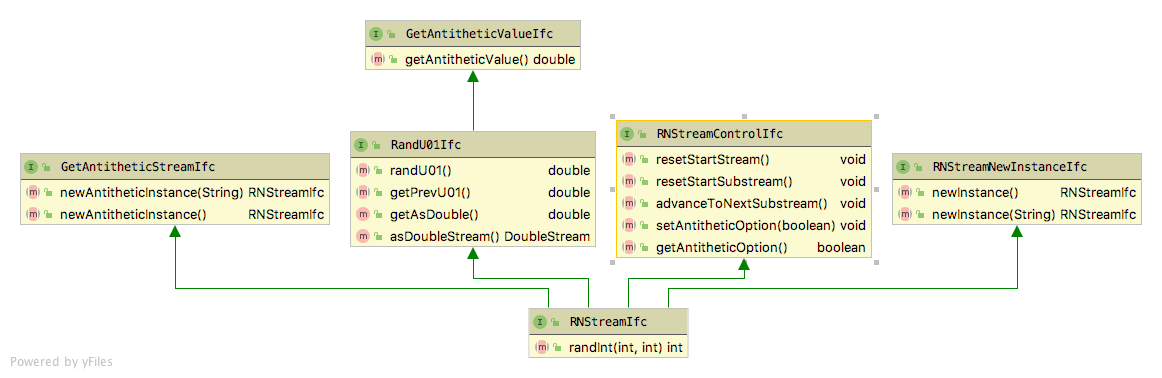
\includegraphics{./figures/RNStreamInterfaces.png}
\caption{\label{fig:RNStreamInterfaces}Random Number Stream Interfaces}
\end{figure}

Figure \ref{fig:RNStreamInterfaces} shows the important interfaces within the
\texttt{jsl.utilities.random.rng} package. The \texttt{RandU01Ifc} defines the methods for
getting the next pseudo-random number and the previous pseudo-random
number via \texttt{randU01()} and \texttt{getPrevU01()}. The \texttt{randInt(int\ i,\ int\ j)} method can be used to generate
a random integer uniformly over the range from \(i\) to \(j\). The methods \texttt{getAsDouble()} and
\texttt{asDoubleStream()} permit the random number stream to act as a Java stream
as defined within the \href{https://docs.oracle.com/javase/8/docs/api/?java/util/stream/Stream.html}{Java Stream API}.
The \texttt{GetAntitheticStreamIfc} and \texttt{RNStreamNewInstanceIfc} interfaces allow a new object
instance to be created from the stream. In the case of the \texttt{GetAntitheticStreamIfc} interface
the created stream will produce antithetic variates from the stream. If \(U\) is a pseudo-random number,
then \(1-U\) is the antithetic variate of \(U\).

The \texttt{RNStreamControlIfc} defines methods for controlling the underlying stream of pseudo-random numbers.

\begin{itemize}
\tightlist
\item
  \texttt{resetStartStream()} - positions the random number generator at the
  beginning of its stream. This is the same location in the stream as
  assigned when the random number generator was created and
  initialized.
\item
  \texttt{resetStartSubstream()} - resets the position of the random number
  generator to the start of the current substream. If the random
  number generator has advanced into the substream, then this method
  resets to the beginning of the substream.
\item
  \texttt{advanceToNextSubStream()} - positions the random number generator at
  the beginning of its next substream. This method move through the
  current substream and positions the generator at the beginning of
  the next substream.
\item
  \texttt{setAntitheticOption(boolean\ flag)} - if the flag is true, the
  generator should start producing antithetic variates with the next
  call to \texttt{randU01()}. If the flag is false, the generator should stop
  producing antithetic variates.
\item
  \texttt{getAntitheticOption()} - returns whether the antithetic option has
  been set.
\end{itemize}

The \texttt{RNStreamIfc} interface assumes that the underlying pseudo-random number generator can produce
multiple streams that can be further divided into substreams. The reset
methods allow the user to move within the streams. Classes that
implement the \texttt{RNStreamControlIfc} can manipulate the streams in a
well-defined manner.

\begin{figure}
\centering
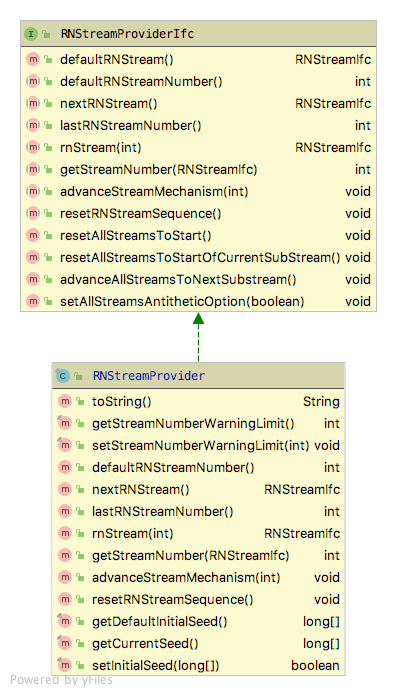
\includegraphics{./figures/RNStreamProvider.png}
\caption{\label{fig:RNStreamProvider}RNStreamProviderIfc Interface}
\end{figure}

To create an concrete instance of a stream, we must have a random number stream provider. This
functionality is defined by the \texttt{RNStreamProviderIfc} interface and its concrete implementation,
\texttt{RNStreamProvider}. Figure \ref{fig:RNStreamProvider} illustrates the functionality available for
creating random number streams. This interface conceptualizes the creation of random number streams
as a process of making a sequence of streams numbered 1, 2, 3, \ldots{}

A random number stream provider must define a default stream, which can be retrieved via the
\texttt{defaultRNStream()} method. For the JSL, the default stream is the first
stream created and is label with the sequence number 1. The sequence number of a stream
can be used to retrieve a particular stream from the provider. The following methods
allow for creation and access to streams.

\begin{itemize}
\tightlist
\item
  \texttt{nextRNStream()} - returns the next random number stream associated with the provider. Each call
  to \texttt{nextRNStream()} makes a new stream in the sequence of streams.
\item
  \texttt{lastRNStreamNumber()} - returns the number of the stream that was last made. This indicates how
  many streams have been made. If \(0\) is returned, then no streams have been made by the provider.
\item
  \texttt{rnStream(int\ k)} - returns the \(k^{th}\) stream. If \(k\) is greater than \texttt{lastRNStreamNumber()} then \texttt{lastRNStreamNumber()} is advanced according to the additional number of streams by creating any intermediate streams. For example, if \texttt{lastRNStreamNumber()} = 10 and k = 15, then streams 11, 12, 13, 14, 15 are assumed provided and stream 15 is returned and \texttt{lastRNStreamNumber()} now equals 15. If \(k\) is less than or equal to \texttt{lastRNStreamNumber()}, then no new streams are created and \texttt{lastRNStreamNumber()}stays at its current value and the \(k^{th}\) stream is returned.
\item
  \texttt{getStreamNumber(RNStreamIfc\ stream)} - returns the stream number of the instance of a stream.
\item
  \texttt{advanceStreamMechanism(int\ n)} - advances the underlying stream mechanism by the specified number of streams, without actually creating the streams. The value of \texttt{lastRNStreamNumber()} remains the same after advancing through
  the streams. In other words, this method should act as if \texttt{nextRNStream()} was not called but advance the underlying stream mechanism as if \(n\) streams had been provided.
\item
  \texttt{resetRNStreamSequence()} - Causes the random number stream provider to act as if has never created any streams. Thus,
  the next call to \texttt{nextRNStream()} will return the \(1^{st}\) stream.
\end{itemize}

The random number stream provider also facilitates the control of all streams that have been created. This functionality is similar to how the position within an individual stream can be manipulated, except the provider performs the functionality on all streams that it has created. The following methods perform this function.

\begin{itemize}
\tightlist
\item
  \texttt{resetAllStreamsToStart()} - resets all created streams to the start of their stream.
\item
  \texttt{resetAllStreamsToStartOfCurrentSubStream()} - resets all created streams to the start of their current sub-stream.
\item
  \texttt{advanceAllStreamsToNextSubstream()} - advances all created streams to the start of their next sub-stream.
\item
  \texttt{setAllStreamsAntitheticOption(boolean\ option)} - changes all created streams to have their antithetic option either off = false or on = true.
\end{itemize}

Many random number generators require the specification of a seed to start the generated sequence. Even though the generator within the JSL use seeds, there really is not any need to utilize the seeds because of the well defined methods for moving within the streams. Now, let's illustrate how to create and manipulate streams.

\hypertarget{ch2:creatingStreams}{%
\subsection{Creating and Using Streams}\label{ch2:creatingStreams}}

To create a random number stream, the user must utilize an instance of \texttt{RNStreamProvider}. This process is illustrated in in the following code. This code creates two instances of \texttt{RNStreamProvider} and gets the first stream from each instance. The instances of \texttt{RNStreamProvider} use the exact same underlying default seeds. Thus, they produce \emph{exactly the same} sequence of streams.



\begin{Shaded}
\begin{Highlighting}[]
\CommentTok{// make a provider for creating streams}
\NormalTok{RNStreamProvider p1 }\OperatorTok{=} \KeywordTok{new} \FunctionTok{RNStreamProvider}\OperatorTok{();}
\CommentTok{// get the first stream from the provider}
\NormalTok{RNStreamIfc p1s1 }\OperatorTok{=}\NormalTok{ p1}\OperatorTok{.}\FunctionTok{nextRNStream}\OperatorTok{();}
\CommentTok{// make another provider, the providers are identical}
\NormalTok{RNStreamProvider p2 }\OperatorTok{=} \KeywordTok{new} \FunctionTok{RNStreamProvider}\OperatorTok{();}
\CommentTok{// thus the first streams returned are identical}
\NormalTok{RNStreamIfc p2s1 }\OperatorTok{=}\NormalTok{ p2}\OperatorTok{.}\FunctionTok{nextRNStream}\OperatorTok{();}
\BuiltInTok{System}\OperatorTok{.}\FunctionTok{out}\OperatorTok{.}\FunctionTok{printf}\OperatorTok{(}\StringTok{"}\SpecialCharTok{\%3s}\StringTok{ }\SpecialCharTok{\%15s}\StringTok{ }\SpecialCharTok{\%15s}\StringTok{ }\SpecialCharTok{\%n}\StringTok{"}\OperatorTok{,} \StringTok{"n"}\OperatorTok{,} \StringTok{"f1s1"}\OperatorTok{,} \StringTok{"f2s2"}\OperatorTok{);}
\ControlFlowTok{for} \OperatorTok{(}\DataTypeTok{int}\NormalTok{ i }\OperatorTok{=} \DecValTok{0}\OperatorTok{;}\NormalTok{ i }\OperatorTok{\textless{}} \DecValTok{5}\OperatorTok{;}\NormalTok{ i}\OperatorTok{++)} \OperatorTok{\{}
    \BuiltInTok{System}\OperatorTok{.}\FunctionTok{out}\OperatorTok{.}\FunctionTok{printf}\OperatorTok{(}\StringTok{"}\SpecialCharTok{\%3d}\StringTok{ }\SpecialCharTok{\%15f}\StringTok{ }\SpecialCharTok{\%15f}\StringTok{ }\SpecialCharTok{\%n}\StringTok{"}\OperatorTok{,}\NormalTok{ i}\OperatorTok{,}\NormalTok{ p1s1}\OperatorTok{.}\FunctionTok{randU01}\OperatorTok{(),}\NormalTok{ p2s1}\OperatorTok{.}\FunctionTok{randU01}\OperatorTok{());}
\OperatorTok{\}}
\end{Highlighting}
\end{Shaded}

Thus, in the following code output, the randomly generated values are exactly the same for the two streams.

\begin{verbatim}
  n            p1s1            p2s2 
  1        0.728510        0.728510 
  2        0.965587        0.965587 
  3        0.996184        0.996184 
  4        0.114988        0.114988 
  5        0.973145        0.973145 
\end{verbatim}

There is is really very little need for the general programmer to create
a \texttt{RNStreamProvider} because the JSL supplies default provider that can be used to provide a
virtually infinite number of streams. The need for directly accessing the functionality of \texttt{RNStreamProvider} is
for very fine control of stream creation in such situations like running
code on different computers in parallel. While the providers produce the
same streams, you can force one provider to be different from another
provider by manipulating the seeds. In addition, the
provider can control all streams that it produces. So, unless you are
trying to do some advanced work that involves coordinating multiple streams, you should not need to create multiple instances of \texttt{RNStreamProvider}.

Because the most common use case is to just have a single provider of streams, the JSL facilitates this through the \texttt{JSLRandom} class. The \texttt{JSLRandom} class has a wide range of static methods to facilitate random variate generation.
The most important methods include:

\begin{itemize}
\tightlist
\item
  \texttt{nextRNStream()} - calls the underlying default \texttt{RNStreamProvider} to create a new random number stream
\item
  \texttt{rnStream(int\ k)} - returns the \(k^{th}\) stream from the default \texttt{RNStreamProvider}
\item
  \texttt{getDefaultRNStream()} - calls the underlying default \texttt{RNStreamProvider} for its default stream
\end{itemize}

In the following code example, these methods are used to create streams that are used to generate random numbers.
The first line of the code uses the static method \texttt{getDefaultRNStream()} of \texttt{JSLRandom} to get the default stream and
then generates three random numbers. The stream is then advanced and three new random numbers are generated. Then,
the stream is reset to its starting (initial seed) and it then repeats the original values. Finally, the a new stream
is created via \texttt{JSLRandom.nextRNStream()} and then used to generate new random numbers. From a conceptual standpoint,
each stream contains an independent sequence of random numbers from any other stream (unless of course they are made from different providers). They are conceptually infinite and independent due to their enormous periods.

\begin{Shaded}
\begin{Highlighting}[]
\NormalTok{RNStreamIfc s1 }\OperatorTok{=}\NormalTok{ JSLRandom}\OperatorTok{.}\FunctionTok{getDefaultRNStream}\OperatorTok{();}
\BuiltInTok{System}\OperatorTok{.}\FunctionTok{out}\OperatorTok{.}\FunctionTok{println}\OperatorTok{(}\StringTok{"Default stream is stream 1"}\OperatorTok{);}
\BuiltInTok{System}\OperatorTok{.}\FunctionTok{out}\OperatorTok{.}\FunctionTok{println}\OperatorTok{(}\StringTok{"Generate 3 random numbers"}\OperatorTok{);}
\ControlFlowTok{for} \OperatorTok{(}\DataTypeTok{int}\NormalTok{ i }\OperatorTok{=} \DecValTok{1}\OperatorTok{;}\NormalTok{ i }\OperatorTok{\textless{}=} \DecValTok{3}\OperatorTok{;}\NormalTok{ i}\OperatorTok{++)} \OperatorTok{\{}
    \BuiltInTok{System}\OperatorTok{.}\FunctionTok{out}\OperatorTok{.}\FunctionTok{println}\OperatorTok{(}\StringTok{"u = "} \OperatorTok{+}\NormalTok{ s1}\OperatorTok{.}\FunctionTok{randU01}\OperatorTok{());}
\OperatorTok{\}}
\NormalTok{s1}\OperatorTok{.}\FunctionTok{advanceToNextSubstream}\OperatorTok{();}
\BuiltInTok{System}\OperatorTok{.}\FunctionTok{out}\OperatorTok{.}\FunctionTok{println}\OperatorTok{(}\StringTok{"Advance to next sub{-}stream and get some more random numbers"}\OperatorTok{);}
\ControlFlowTok{for} \OperatorTok{(}\DataTypeTok{int}\NormalTok{ i }\OperatorTok{=} \DecValTok{1}\OperatorTok{;}\NormalTok{ i }\OperatorTok{\textless{}=} \DecValTok{3}\OperatorTok{;}\NormalTok{ i}\OperatorTok{++)} \OperatorTok{\{}
    \BuiltInTok{System}\OperatorTok{.}\FunctionTok{out}\OperatorTok{.}\FunctionTok{println}\OperatorTok{(}\StringTok{"u = "} \OperatorTok{+}\NormalTok{ s1}\OperatorTok{.}\FunctionTok{randU01}\OperatorTok{());}
\OperatorTok{\}}
\BuiltInTok{System}\OperatorTok{.}\FunctionTok{out}\OperatorTok{.}\FunctionTok{println}\OperatorTok{(}\StringTok{"Notice that they are different from the first 3."}\OperatorTok{);}
\NormalTok{s1}\OperatorTok{.}\FunctionTok{resetStartStream}\OperatorTok{();}
\BuiltInTok{System}\OperatorTok{.}\FunctionTok{out}\OperatorTok{.}\FunctionTok{println}\OperatorTok{(}\StringTok{"Reset the stream to the beginning of its sequence"}\OperatorTok{);}
\ControlFlowTok{for} \OperatorTok{(}\DataTypeTok{int}\NormalTok{ i }\OperatorTok{=} \DecValTok{1}\OperatorTok{;}\NormalTok{ i }\OperatorTok{\textless{}=} \DecValTok{3}\OperatorTok{;}\NormalTok{ i}\OperatorTok{++)} \OperatorTok{\{}
    \BuiltInTok{System}\OperatorTok{.}\FunctionTok{out}\OperatorTok{.}\FunctionTok{println}\OperatorTok{(}\StringTok{"u = "} \OperatorTok{+}\NormalTok{ s1}\OperatorTok{.}\FunctionTok{randU01}\OperatorTok{());}
\OperatorTok{\}}
\BuiltInTok{System}\OperatorTok{.}\FunctionTok{out}\OperatorTok{.}\FunctionTok{println}\OperatorTok{(}\StringTok{"Notice that they are the same as the first 3."}\OperatorTok{);}
\BuiltInTok{System}\OperatorTok{.}\FunctionTok{out}\OperatorTok{.}\FunctionTok{println}\OperatorTok{(}\StringTok{"Get another random number stream"}\OperatorTok{);}
\NormalTok{RNStreamIfc s2 }\OperatorTok{=}\NormalTok{ JSLRandom}\OperatorTok{.}\FunctionTok{nextRNStream}\OperatorTok{();}
\BuiltInTok{System}\OperatorTok{.}\FunctionTok{out}\OperatorTok{.}\FunctionTok{println}\OperatorTok{(}\StringTok{"2nd stream"}\OperatorTok{);}
\ControlFlowTok{for} \OperatorTok{(}\DataTypeTok{int}\NormalTok{ i }\OperatorTok{=} \DecValTok{1}\OperatorTok{;}\NormalTok{ i }\OperatorTok{\textless{}=} \DecValTok{3}\OperatorTok{;}\NormalTok{ i}\OperatorTok{++)} \OperatorTok{\{}
    \BuiltInTok{System}\OperatorTok{.}\FunctionTok{out}\OperatorTok{.}\FunctionTok{println}\OperatorTok{(}\StringTok{"u = "} \OperatorTok{+}\NormalTok{ s2}\OperatorTok{.}\FunctionTok{randU01}\OperatorTok{());}
\OperatorTok{\}}
\BuiltInTok{System}\OperatorTok{.}\FunctionTok{out}\OperatorTok{.}\FunctionTok{println}\OperatorTok{(}\StringTok{"Notice that they are different from the first 3."}\OperatorTok{);}
\end{Highlighting}
\end{Shaded}

The resulting output from this code is as follows. Again, the methods of the \texttt{RNStreamControlIfc} interface that permit movement within a stream are extremely useful for controlling the randomness associated with a simulation.

\begin{verbatim}
Default stream is stream 1
Generate 3 random numbers
u = 0.12701112204657714
u = 0.3185275653967945
u = 0.3091860155832701
Advance to next sub-stream and get some more random numbers
u = 0.07939898979733463
u = 0.4803395047575741
u = 0.8583222470551328
Notice that they are different from the first 3.
Reset the stream to the beginning of its sequence
u = 0.12701112204657714
u = 0.3185275653967945
u = 0.3091860155832701
Notice that they are the same as the first 3.
Get another random number stream
2nd stream
u = 0.7285097861965271
u = 0.9655872822837334
u = 0.9961841304801171
Notice that they are different from the first 3.
\end{verbatim}

\hypertarget{ch2:crn}{%
\subsection{Common Random Numbers}\label{ch2:crn}}

Common random numbers (CRN) is a Monte Carlo method that has different experiments utilize the same random numbers. CRN is a variance reduction technique that allows the experimenter to block out the effect of the random numbers used in the experiment. To facilitate the use of common random numbers the JSL has the aforementioned stream control mechanism. One way to implement common random numbers is to use two instances of \texttt{RNStreamProvider} as was previously illustrated. In that case, the two providers produce the same sequence of streams and thus those streams can be used on the different experiments. An alternative method that does not require the use of two providers is to create a copy of the stream directly from the stream instance. The following code clones the stream instance.

\begin{Shaded}
\begin{Highlighting}[]
\CommentTok{// get the default stream}
\NormalTok{RNStreamIfc s }\OperatorTok{=}\NormalTok{ JSLRandom}\OperatorTok{.}\FunctionTok{getDefaultRNStream}\OperatorTok{();}
\CommentTok{// make a clone of the stream}
\NormalTok{RNStreamIfc clone }\OperatorTok{=}\NormalTok{ s}\OperatorTok{.}\FunctionTok{newInstance}\OperatorTok{();}
\BuiltInTok{System}\OperatorTok{.}\FunctionTok{out}\OperatorTok{.}\FunctionTok{printf}\OperatorTok{(}\StringTok{"}\SpecialCharTok{\%3s}\StringTok{ }\SpecialCharTok{\%15s}\StringTok{ }\SpecialCharTok{\%15s}\StringTok{ }\SpecialCharTok{\%n}\StringTok{"}\OperatorTok{,} \StringTok{"n"}\OperatorTok{,} \StringTok{"U"}\OperatorTok{,} \StringTok{"U again"}\OperatorTok{);}
\ControlFlowTok{for} \OperatorTok{(}\DataTypeTok{int}\NormalTok{ i }\OperatorTok{=} \DecValTok{0}\OperatorTok{;}\NormalTok{ i }\OperatorTok{\textless{}} \DecValTok{3}\OperatorTok{;}\NormalTok{ i}\OperatorTok{++)} \OperatorTok{\{}
    \BuiltInTok{System}\OperatorTok{.}\FunctionTok{out}\OperatorTok{.}\FunctionTok{printf}\OperatorTok{(}\StringTok{"}\SpecialCharTok{\%3d}\StringTok{ }\SpecialCharTok{\%15f}\StringTok{ }\SpecialCharTok{\%15f}\StringTok{ }\SpecialCharTok{\%n}\StringTok{"}\OperatorTok{,}\NormalTok{ i}\OperatorTok{+}\DecValTok{1}\OperatorTok{,}\NormalTok{ s}\OperatorTok{.}\FunctionTok{randU01}\OperatorTok{(),}\NormalTok{ clone}\OperatorTok{.}\FunctionTok{randU01}\OperatorTok{());}
\OperatorTok{\}}
\end{Highlighting}
\end{Shaded}

Since the instances have the same underlying state, they produce the same random numbers. Please note that the cloned stream instance is not produced by the underlying \texttt{RNStreamProvider} and thus it is not part of the set of streams managed or controlled by the provider.

\begin{verbatim}
  n               U         U again 
  1        0.127011        0.127011 
  2        0.318528        0.318528 
  3        0.309186        0.309186 
\end{verbatim}

An alternative method is to just use the \texttt{resetStartStream()} method of the stream to reset the stream to the desired location in its sequence and then reproduce the random numbers. This is illustrated in the following code.

\begin{Shaded}
\begin{Highlighting}[]
\NormalTok{RNStreamIfc s }\OperatorTok{=}\NormalTok{ JSLRandom}\OperatorTok{.}\FunctionTok{getDefaultRNStream}\OperatorTok{();}
\CommentTok{// generate regular}
\BuiltInTok{System}\OperatorTok{.}\FunctionTok{out}\OperatorTok{.}\FunctionTok{printf}\OperatorTok{(}\StringTok{"}\SpecialCharTok{\%3s}\StringTok{ }\SpecialCharTok{\%15s}\StringTok{ }\SpecialCharTok{\%n}\StringTok{"}\OperatorTok{,} \StringTok{"n"}\OperatorTok{,} \StringTok{"U"}\OperatorTok{);}
\ControlFlowTok{for} \OperatorTok{(}\DataTypeTok{int}\NormalTok{ i }\OperatorTok{=} \DecValTok{0}\OperatorTok{;}\NormalTok{ i }\OperatorTok{\textless{}} \DecValTok{3}\OperatorTok{;}\NormalTok{ i}\OperatorTok{++)} \OperatorTok{\{}
    \DataTypeTok{double}\NormalTok{ u }\OperatorTok{=}\NormalTok{ s}\OperatorTok{.}\FunctionTok{randU01}\OperatorTok{();}
    \BuiltInTok{System}\OperatorTok{.}\FunctionTok{out}\OperatorTok{.}\FunctionTok{printf}\OperatorTok{(}\StringTok{"}\SpecialCharTok{\%3d}\StringTok{ }\SpecialCharTok{\%15f}\StringTok{ }\SpecialCharTok{\%n}\StringTok{"}\OperatorTok{,}\NormalTok{ i}\OperatorTok{+}\DecValTok{1}\OperatorTok{,}\NormalTok{ u}\OperatorTok{);}
\OperatorTok{\}}
\CommentTok{// reset the stream and generate again}
\NormalTok{s}\OperatorTok{.}\FunctionTok{resetStartStream}\OperatorTok{();}
\BuiltInTok{System}\OperatorTok{.}\FunctionTok{out}\OperatorTok{.}\FunctionTok{println}\OperatorTok{();}
\BuiltInTok{System}\OperatorTok{.}\FunctionTok{out}\OperatorTok{.}\FunctionTok{printf}\OperatorTok{(}\StringTok{"}\SpecialCharTok{\%3s}\StringTok{ }\SpecialCharTok{\%15s}\StringTok{ }\SpecialCharTok{\%n}\StringTok{"}\OperatorTok{,} \StringTok{"n"}\OperatorTok{,} \StringTok{"U again"}\OperatorTok{);}
\ControlFlowTok{for} \OperatorTok{(}\DataTypeTok{int}\NormalTok{ i }\OperatorTok{=} \DecValTok{0}\OperatorTok{;}\NormalTok{ i }\OperatorTok{\textless{}} \DecValTok{3}\OperatorTok{;}\NormalTok{ i}\OperatorTok{++)} \OperatorTok{\{}
    \DataTypeTok{double}\NormalTok{ u }\OperatorTok{=}\NormalTok{ s}\OperatorTok{.}\FunctionTok{randU01}\OperatorTok{();}
    \BuiltInTok{System}\OperatorTok{.}\FunctionTok{out}\OperatorTok{.}\FunctionTok{printf}\OperatorTok{(}\StringTok{"}\SpecialCharTok{\%3d}\StringTok{ }\SpecialCharTok{\%15f}\StringTok{ }\SpecialCharTok{\%n}\StringTok{"}\OperatorTok{,}\NormalTok{ i}\OperatorTok{+}\DecValTok{1}\OperatorTok{,}\NormalTok{ u}\OperatorTok{);}
\OperatorTok{\}}
\end{Highlighting}
\end{Shaded}

Notice that the generated numbers are the same.

\begin{verbatim}
  n               U 
  1        0.127011 
  2        0.318528 
  3        0.309186 

  n         U again 
  1        0.127011 
  2        0.318528 
  3        0.309186 
\end{verbatim}

Thus, a experiment can be executed, then the random numbers reset to the desired location. Then, by changing the experimental conditions and re-running the simulation, the same random numbers are used. If many streams are used, then by accessing the \texttt{RNStreamProvider} you can reset all of the controlled streams with one call and then perform the next experiment.

\hypertarget{ch2:antitheticStreams}{%
\subsection{Creating and Using Antithetic Streams}\label{ch2:antitheticStreams}}

Recall that if a pseudo-random number is called \(U\) then its antithetic value is \(1-U\). There are a number of methods to access antithetic values. The simplest is to create an antithetic instance from a given stream. This is illustrated is in the following code. Please note that the antithetic stream instance is not produced by the underlying \texttt{RNStreamProvider} and thus it is not part of the set of streams managed or controlled by the provider. The new instance process directly creates the new stream based on the current stream so that it has the same underling state and it is set to produce antithetic values.

\begin{Shaded}
\begin{Highlighting}[]
\CommentTok{// get the default stream}
\NormalTok{RNStreamIfc s }\OperatorTok{=}\NormalTok{ JSLRandom}\OperatorTok{.}\FunctionTok{getDefaultRNStream}\OperatorTok{();}
\CommentTok{// make its antithetic version}
\NormalTok{RNStreamIfc as }\OperatorTok{=}\NormalTok{ s}\OperatorTok{.}\FunctionTok{newAntitheticInstance}\OperatorTok{();}
\BuiltInTok{System}\OperatorTok{.}\FunctionTok{out}\OperatorTok{.}\FunctionTok{printf}\OperatorTok{(}\StringTok{"}\SpecialCharTok{\%3s}\StringTok{ }\SpecialCharTok{\%15s}\StringTok{ }\SpecialCharTok{\%15s}\StringTok{ }\SpecialCharTok{\%15s}\StringTok{ }\SpecialCharTok{\%n}\StringTok{"}\OperatorTok{,} \StringTok{"n"}\OperatorTok{,} \StringTok{"U"}\OperatorTok{,} \StringTok{"1{-}U"}\OperatorTok{,} \StringTok{"sum"}\OperatorTok{);}
\ControlFlowTok{for} \OperatorTok{(}\DataTypeTok{int}\NormalTok{ i }\OperatorTok{=} \DecValTok{0}\OperatorTok{;}\NormalTok{ i }\OperatorTok{\textless{}} \DecValTok{5}\OperatorTok{;}\NormalTok{ i}\OperatorTok{++)} \OperatorTok{\{}
    \DataTypeTok{double}\NormalTok{ u }\OperatorTok{=}\NormalTok{ s}\OperatorTok{.}\FunctionTok{randU01}\OperatorTok{();}
    \DataTypeTok{double}\NormalTok{ au }\OperatorTok{=}\NormalTok{ as}\OperatorTok{.}\FunctionTok{randU01}\OperatorTok{();}
    \BuiltInTok{System}\OperatorTok{.}\FunctionTok{out}\OperatorTok{.}\FunctionTok{printf}\OperatorTok{(}\StringTok{"}\SpecialCharTok{\%3d}\StringTok{ }\SpecialCharTok{\%15f}\StringTok{ }\SpecialCharTok{\%15f}\StringTok{ }\SpecialCharTok{\%15f}\StringTok{ }\SpecialCharTok{\%n}\StringTok{"}\OperatorTok{,}\NormalTok{ i}\OperatorTok{+}\DecValTok{1}\OperatorTok{,}\NormalTok{ u}\OperatorTok{,}\NormalTok{ au}\OperatorTok{,} \OperatorTok{(}\NormalTok{u}\OperatorTok{+}\NormalTok{au}\OperatorTok{));}
\OperatorTok{\}}
\end{Highlighting}
\end{Shaded}

Notice that the generated values sum to 1.0.

\begin{verbatim}
  n               U             1-U             sum 
  1        0.127011        0.872989        1.000000 
  2        0.318528        0.681472        1.000000 
  3        0.309186        0.690814        1.000000 
  4        0.825847        0.174153        1.000000 
  5        0.221630        0.778370        1.000000 
\end{verbatim}

An alternate method that does not require the creation of another stream involves using the \texttt{resetStartStream()} and \texttt{setAntitheticOption(boolean\ flag)} methods of the current stream. If you have a stream, you can use the \texttt{setAntitheticOption(boolean\ flag)} to cause the stream to start producing antithetic values. If you use the \texttt{resetStartStream()} method and then set the antithetic option to true, the stream will be set to its initial starting point and then produce antithetic values.

\begin{Shaded}
\begin{Highlighting}[]
\NormalTok{RNStreamIfc s }\OperatorTok{=}\NormalTok{ JSLRandom}\OperatorTok{.}\FunctionTok{getDefaultRNStream}\OperatorTok{();}
\CommentTok{// generate regular}
\BuiltInTok{System}\OperatorTok{.}\FunctionTok{out}\OperatorTok{.}\FunctionTok{printf}\OperatorTok{(}\StringTok{"}\SpecialCharTok{\%3s}\StringTok{ }\SpecialCharTok{\%15s}\StringTok{ }\SpecialCharTok{\%n}\StringTok{"}\OperatorTok{,} \StringTok{"n"}\OperatorTok{,} \StringTok{"U"}\OperatorTok{);}
\ControlFlowTok{for} \OperatorTok{(}\DataTypeTok{int}\NormalTok{ i }\OperatorTok{=} \DecValTok{0}\OperatorTok{;}\NormalTok{ i }\OperatorTok{\textless{}} \DecValTok{5}\OperatorTok{;}\NormalTok{ i}\OperatorTok{++)} \OperatorTok{\{}
    \DataTypeTok{double}\NormalTok{ u }\OperatorTok{=}\NormalTok{ s}\OperatorTok{.}\FunctionTok{randU01}\OperatorTok{();}
    \BuiltInTok{System}\OperatorTok{.}\FunctionTok{out}\OperatorTok{.}\FunctionTok{printf}\OperatorTok{(}\StringTok{"}\SpecialCharTok{\%3d}\StringTok{ }\SpecialCharTok{\%15f}\StringTok{ }\SpecialCharTok{\%n}\StringTok{"}\OperatorTok{,}\NormalTok{ i}\OperatorTok{+}\DecValTok{1}\OperatorTok{,}\NormalTok{ u}\OperatorTok{);}
\OperatorTok{\}}
\CommentTok{// generate antithetic}
\NormalTok{s}\OperatorTok{.}\FunctionTok{resetStartStream}\OperatorTok{();}
\NormalTok{s}\OperatorTok{.}\FunctionTok{setAntitheticOption}\OperatorTok{(}\KeywordTok{true}\OperatorTok{);}
\BuiltInTok{System}\OperatorTok{.}\FunctionTok{out}\OperatorTok{.}\FunctionTok{println}\OperatorTok{();}
\BuiltInTok{System}\OperatorTok{.}\FunctionTok{out}\OperatorTok{.}\FunctionTok{printf}\OperatorTok{(}\StringTok{"}\SpecialCharTok{\%3s}\StringTok{ }\SpecialCharTok{\%15s}\StringTok{ }\SpecialCharTok{\%n}\StringTok{"}\OperatorTok{,} \StringTok{"n"}\OperatorTok{,} \StringTok{"1{-}U"}\OperatorTok{);}
\ControlFlowTok{for} \OperatorTok{(}\DataTypeTok{int}\NormalTok{ i }\OperatorTok{=} \DecValTok{0}\OperatorTok{;}\NormalTok{ i }\OperatorTok{\textless{}} \DecValTok{5}\OperatorTok{;}\NormalTok{ i}\OperatorTok{++)} \OperatorTok{\{}
    \DataTypeTok{double}\NormalTok{ u }\OperatorTok{=}\NormalTok{ s}\OperatorTok{.}\FunctionTok{randU01}\OperatorTok{();}
    \BuiltInTok{System}\OperatorTok{.}\FunctionTok{out}\OperatorTok{.}\FunctionTok{printf}\OperatorTok{(}\StringTok{"}\SpecialCharTok{\%3d}\StringTok{ }\SpecialCharTok{\%15f}\StringTok{ }\SpecialCharTok{\%n}\StringTok{"}\OperatorTok{,}\NormalTok{ i}\OperatorTok{+}\DecValTok{1}\OperatorTok{,}\NormalTok{ u}\OperatorTok{);}
\OperatorTok{\}}
\end{Highlighting}
\end{Shaded}

Notice that the second set of random numbers is the complement of the first set in this output. Of course, you can also create multiple instances of \texttt{RNStreamProvider}, and then create streams and set one of the streams to produce antithetic values.

\begin{verbatim}
  n               U 
  1        0.127011 
  2        0.318528 
  3        0.309186 
  4        0.825847 
  5        0.221630
  
  n             1-U 
  1        0.872989 
  2        0.681472 
  3        0.690814 
  4        0.174153 
  5        0.778370
\end{verbatim}

\hypertarget{ch2:FAQ}{%
\section{Frequently Asked Questions}\label{ch2:FAQ}}

\begin{enumerate}
\def\labelenumi{\arabic{enumi}.}
\item
  \textbf{What are pseudo-random numbers?}
  Numbers generated through an algorithm that appear to be random, when in fact, they are created by a deterministic process.
\item
  \textbf{Why do we want to control randomness within simulation models?}
  By controlling randomness, we can better ascertain if changes in simulation responses are due to factors of interest or due to underlying statistical variation caused by sampling. Do you think that it is better to compare two systems using the same inputs or different inputs? Suppose we have a work process that we have redesigned. We have the old process and the new process. Would it be better to test the difference in the process by using two different workers or the same worker? Most people agree that using the same worker is better. This same logic applies to randomness. Since we can control which pseudo-random number we use, it is better to test the difference between two model alternatives by using the same pseudo-random numbers. We use seeds and streams to do this.
\item
  \textbf{What are seeds and streams?}
  A random number stream is a sub-sequence of pseudo-random numbers that start at particular place with a larger sequence of pseudo-random numbers. The starting point of a sequence of pseudo-random numbers is called the seed. A seed allows us to pick a particular stream. Having multiple streams is useful to assign different streams to different sources of randomness within a model. This facilitates the control of the use of pseudo-random numbers when performing experiments.
\item
  \textbf{How come my simulation results are always the same?}
  Random number generators in computer simulation languages come with a default set of streams that divide the ``circle'' up into independent sets of random numbers. The streams are only independent if you do not use up all the random numbers within the subsequence. These streams allow the randomness associated with a simulation to be controlled. During the simulation, you can associate a specific stream with specific random processes in the model. This has the advantage of allowing you to check if the random numbers are causing significant differences in the outputs. In addition, this allows the random numbers used across alternative simulations to be better synchronized.
  Now a common question in simulation can be answered. That is, ``If the simulation is using random numbers, why to I get the same results each time I run my program?'' The corollary to this question is, ``If I want to get different random results each time I run my program, how do I do it?'' The answer to the first question is that the underlying random number generator is starting with the same seed each time you run your program. Thus, your program will use the same pseudo random numbers today as it did yesterday and the day before, etc. The answer to the corollary question is that you must tell the random number generator to use a different seed (or alternatively a different stream) if you want different invocations of the program to produce different results. The latter is not necessarily a desirable goal. For example, when developing your simulation programs, it is desirable to have repeatable results so that you can know that your program is working correctly.
\item
  \textbf{How come my simulation results are unexpectedly different?}
  Sometimes by changing the order of method calls you change the sequence of random numbers that are assigned to various things that happen in the model (e.g.~attribute, generated service times, paths taken, etc.). Please see the FAQ ``How come my results are always the same?''. Now, the result can sometimes be radically different if different random numbers are used for different purposes. By using streams, you reduce this possibility and increase the likelihood that two models that have different configurations will have differences due to the change and not due to the random numbers used.
\end{enumerate}

\hypertarget{random-variate-generation-and-probability-modeling}{%
\chapter{Random Variate Generation and Probability Modeling}\label{random-variate-generation-and-probability-modeling}}

\textbf{\textsc{Learning Objectives}}

\begin{itemize}
\item
  To be able to generate random variates using the Java Simulation
  Library (JSL)
\item
\begin{verbatim}
To understand how to use the JSL for basic probability computations
\end{verbatim}
\end{itemize}

The JSL has the capability to generate random variates from both
discrete and continuous distributions. The \href{https://rossetti.git-pages.uark.edu/JSL-Documentation/jsl/utilities/random/rvariable/package-summary.html}{\texttt{jsl.utilities.random.rvariable}} package supports this functionality. The package has a set of Java interfaces
that define the behavior associated with random variables. Concrete
sub-classes of specific random variables are created by sub-classing
\texttt{AbstractRVariable}. As shown in Figure \ref{fig:RVariableIfc}, every random variable has
access to an object that implements the \texttt{RNStreamIfc} interface. This
gives it the ability to generate pseudo-random numbers and to control
the streams. The \texttt{GetValueIfc} interface is the key interface because in
this context it returns a random value from the random variable. For
example, if \texttt{d} is a reference to an instance of a sub-class of type
\texttt{AbstractRVariable}, then \texttt{d.getValue()} generates a random value.

\begin{figure}
\centering
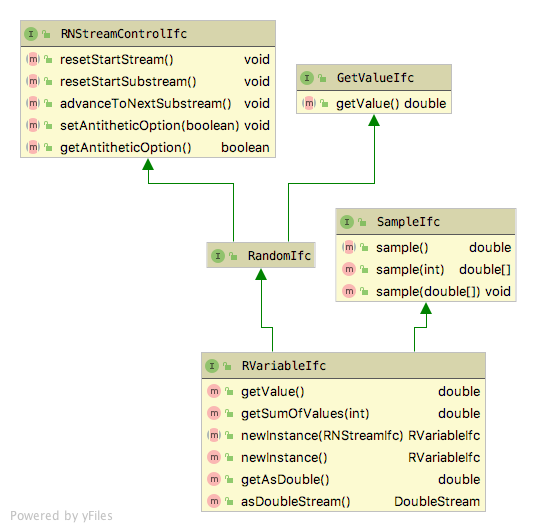
\includegraphics{./figures/RVariableIfc.png}
\caption{\label{fig:RVariableIfc}Random Variable Interfaces}
\end{figure}

\hypertarget{continuous-and-discrete-random-variables}{%
\section{Continuous and Discrete Random Variables}\label{continuous-and-discrete-random-variables}}

The names and parameters associated with the continuous random variables
are as follows:

\begin{itemize}
\tightlist
\item
  BetaRV(double alpha1, double alpha2)
\item
  ChiSquaredRV(double degressOfFreedom)
\item
  ExponentialRV(double mean)
\item
  GammaRV(double shape, double scale)
\item
  GeneralizedBetaRV(double alpha1, double alpha2, double min, double max)
\item
  JohnsonBRV(double alpha1, double alpha2, double min, double max)
\item
  LaplaceRV(double mean, double scale)
\item
  LogLogisticRV(double shape, double scale)
\item
  LognormalRV(double mean, double variance)
\item
  NormalRV(double mean, double variance)
\item
  PearsonType5RV(double shape, double scale)
\item
  PearsonType6RV(double alpha1, double alpha2, double beta)
\item
  StudentTRV(double dof)
\item
  TriangularRV(double min, double mode, double max)
\item
  UniformRV(double lowerLimit, double upperLimit)
\item
  WeibullRV(double shape, double scale)
\end{itemize}

The names and parameters associated with the discrete random variables
are as follows:

\begin{itemize}
\tightlist
\item
  BernoulliRV(double prob)
\item
  BinomialRV(double prob, int numTrials)
\item
  ConstantRV(double value), a degenerate probability mass on a single
  value that cannot be changed
\item
  DEmpiricalRV(double{[}{]} value, double{[}{]} cdf), the value array
  holds the values that can be returned, while the cdf array holds the
  cumulative probabilities associated with the values
\item
  DUniformRV(int minimum, int maximum)
\item
  GeometricRV(double prob), range is 0 to infinity
\item
  NegativeBinomialRV(double prob, double numSuccess), range is 0 to
  infinity. The number of failures befor the \(r^{th}\) success.
\item
  PoissonRV(double mean)
\item
  ShiftedGeometricRV(double prob), range is 1 to infinity
\item
  VConstantRV(double value), a degenerate probability mass on a single
  value that can be changed
\end{itemize}

\hypertarget{overview-of-generation-algorithms}{%
\section{Overview of Generation Algorithms}\label{overview-of-generation-algorithms}}

As you can see, the name of the distribution followed by the letters RV designate the class names. Implementations of these classes extend the \texttt{AbstractRVarable} class, which implements the \texttt{RVariableIfc} interface. Users simply create and instance of the class and then use it to get a sequence of values that have the named probability distribution. In order to implement a new random variable (i.e.~some random variable
that is not already implemented) you can extend the class
\texttt{AbstractRVariable}. This provides a basic template for what is expected
in the implementation. However, it implies that you need to implement
all of the required interfaces. The key method to implement is the
protected \texttt{generate()} method, which should return the generated random
value.

In almost all cases, the JSL utilizes the inverse transform method for generating random variates. Thus, there is a one to one mapping of the underlying pseudo-random number and the resulting random variate. Even in the case of distributions that do not have closed form inverse cumulative distribution functions, the JSL utilizes numerical methods to approximate the function whenever feasible. For example, the JSL uses a rational function approximation, see Cody (1969), to
implement the inverse cumulative distribution function for the standard
normal distribution. The inversion for the gamma distribution is based
on Algorithm AS 91 for inverting the chi-squared distribution and
exploiting its relationship with the gamma. The beta distribution also
uses numerical methods to compute the cumulative distribution function
as well as bi-section search to determine the inverse for cumulative
distribution function.

The JSL implements the \texttt{BernoulliRV}, \texttt{DUniformRV}, \texttt{GeometricRV},
\texttt{NegativeBinomialRV}, and \texttt{ShiftedGeometricRV} classes using the methods
described in Chapter 2 of \citet{Rossetti2015}. While more efficient methods may be available, the
\texttt{PoissonRV} and \texttt{BinomialRV} distributions are implemented by searching the
probability mass functions. Both search methods use an approximation to
get close to the value of the inverse and then search up or down through
the cumulative distribution function. Because of this both distributions
use numerically stable methods to compute the cumulative distribution
function values. The \texttt{DEmpiricalRV} class also searches through the
cumulative distribution function.

\hypertarget{creating-and-using-random-variables}{%
\section{Creating and Using Random Variables}\label{creating-and-using-random-variables}}

The following example code illustrates how to create a normal random variable and how to generate values.

\begin{Shaded}
\begin{Highlighting}[]
\CommentTok{// create a normal mean = 20.0, variance = 4.0 random variable}
\NormalTok{NormalRV n }\OperatorTok{=} \KeywordTok{new} \FunctionTok{NormalRV}\OperatorTok{(}\FloatTok{20.0}\OperatorTok{,} \FloatTok{4.0}\OperatorTok{);}
\BuiltInTok{System}\OperatorTok{.}\FunctionTok{out}\OperatorTok{.}\FunctionTok{printf}\OperatorTok{(}\StringTok{"}\SpecialCharTok{\%3s}\StringTok{ }\SpecialCharTok{\%15s}\StringTok{ }\SpecialCharTok{\%n}\StringTok{"}\OperatorTok{,} \StringTok{"n"}\OperatorTok{,} \StringTok{"Values"}\OperatorTok{);}
\CommentTok{// generate some values}
\ControlFlowTok{for} \OperatorTok{(}\DataTypeTok{int}\NormalTok{ i }\OperatorTok{=} \DecValTok{0}\OperatorTok{;}\NormalTok{ i }\OperatorTok{\textless{}} \DecValTok{5}\OperatorTok{;}\NormalTok{ i}\OperatorTok{++)} \OperatorTok{\{}
    \CommentTok{// getValue() method returns generated values}
    \DataTypeTok{double}\NormalTok{ x }\OperatorTok{=}\NormalTok{ n}\OperatorTok{.}\FunctionTok{getValue}\OperatorTok{();}
    \BuiltInTok{System}\OperatorTok{.}\FunctionTok{out}\OperatorTok{.}\FunctionTok{printf}\OperatorTok{(}\StringTok{"}\SpecialCharTok{\%3d}\StringTok{ }\SpecialCharTok{\%15f}\StringTok{ }\SpecialCharTok{\%n}\StringTok{"}\OperatorTok{,}\NormalTok{ i}\OperatorTok{+}\DecValTok{1}\OperatorTok{,}\NormalTok{ x}\OperatorTok{);}
\OperatorTok{\}}
\end{Highlighting}
\end{Shaded}

The resulting output is what you would expect.

\begin{verbatim}
  n          Values 
  1       21.216624 
  2       23.639128 
  3       25.335884 
  4       17.599163 
  5       23.858350 
\end{verbatim}

Alternatively, the user can use the \texttt{sample()} method to generate an array of values that can be later processed. The following code illustrates how to do that with a triangular distribution.

\begin{Shaded}
\begin{Highlighting}[]
\CommentTok{// create a triangular random variable with min = 2.0, mode = 5.0, max = 10.0}
\NormalTok{TriangularRV t }\OperatorTok{=} \KeywordTok{new} \FunctionTok{TriangularRV}\OperatorTok{(}\FloatTok{2.0}\OperatorTok{,} \FloatTok{5.0}\OperatorTok{,} \FloatTok{10.0}\OperatorTok{);}
\CommentTok{// sample 5 values}
\DataTypeTok{double}\OperatorTok{[]}\NormalTok{ sample }\OperatorTok{=}\NormalTok{ t}\OperatorTok{.}\FunctionTok{sample}\OperatorTok{(}\DecValTok{5}\OperatorTok{);}
\BuiltInTok{System}\OperatorTok{.}\FunctionTok{out}\OperatorTok{.}\FunctionTok{printf}\OperatorTok{(}\StringTok{"}\SpecialCharTok{\%3s}\StringTok{ }\SpecialCharTok{\%15s}\StringTok{ }\SpecialCharTok{\%n}\StringTok{"}\OperatorTok{,} \StringTok{"n"}\OperatorTok{,} \StringTok{"Values"}\OperatorTok{);}
\ControlFlowTok{for} \OperatorTok{(}\DataTypeTok{int}\NormalTok{ i }\OperatorTok{=} \DecValTok{0}\OperatorTok{;}\NormalTok{ i }\OperatorTok{\textless{}}\NormalTok{ sample}\OperatorTok{.}\FunctionTok{length}\OperatorTok{;}\NormalTok{ i}\OperatorTok{++)} \OperatorTok{\{}
    \BuiltInTok{System}\OperatorTok{.}\FunctionTok{out}\OperatorTok{.}\FunctionTok{printf}\OperatorTok{(}\StringTok{"}\SpecialCharTok{\%3d}\StringTok{ }\SpecialCharTok{\%15f}\StringTok{ }\SpecialCharTok{\%n}\StringTok{"}\OperatorTok{,}\NormalTok{ i}\OperatorTok{+}\DecValTok{1}\OperatorTok{,}\NormalTok{ sample}\OperatorTok{[}\NormalTok{i}\OperatorTok{]);}
\OperatorTok{\}}
\end{Highlighting}
\end{Shaded}

Again, the output is what we would expect.

\begin{verbatim}
  n          Values 
  1        3.515540 
  2        6.327783 
  3        4.382075 
  4        7.392228 
  5        8.409238 
\end{verbatim}

It is important to note that the full range of functionality related to stream control is also available for random variables. That is, the underlying stream can be reset to its start, can be advanced to the next substream, can generate antithetic variates, etc. Each new instance of a random variable is supplied with its own unique stream that is not shared with another other random variable instances. Since this underlying random number generator has an enormous number of streams, approximately \(1.8 \times 10^{19}\), it is very unlikely that the user will create so many streams as to start reusing them. However, the streams that are used by random variable instances can be supplied directly so that they may be shared. The following following code example illustrates how to assign a specific stream by passing a specific stream instance into the constructor of the random variable.

\begin{Shaded}
\begin{Highlighting}[]
\CommentTok{// get stream 3}
\NormalTok{RNStreamIfc stream }\OperatorTok{=}\NormalTok{ JSLRandom}\OperatorTok{.}\FunctionTok{rnStream}\OperatorTok{(}\DecValTok{3}\OperatorTok{);}
\CommentTok{// create a normal mean = 20.0, variance = 4.0, with the stream}
\NormalTok{NormalRV n }\OperatorTok{=} \KeywordTok{new} \FunctionTok{NormalRV}\OperatorTok{(}\FloatTok{20.0}\OperatorTok{,} \FloatTok{4.0}\OperatorTok{,}\NormalTok{ stream}\OperatorTok{);}
\BuiltInTok{System}\OperatorTok{.}\FunctionTok{out}\OperatorTok{.}\FunctionTok{printf}\OperatorTok{(}\StringTok{"}\SpecialCharTok{\%3s}\StringTok{ }\SpecialCharTok{\%15s}\StringTok{ }\SpecialCharTok{\%n}\StringTok{"}\OperatorTok{,} \StringTok{"n"}\OperatorTok{,} \StringTok{"Values"}\OperatorTok{);}
\ControlFlowTok{for} \OperatorTok{(}\DataTypeTok{int}\NormalTok{ i }\OperatorTok{=} \DecValTok{0}\OperatorTok{;}\NormalTok{ i }\OperatorTok{\textless{}} \DecValTok{5}\OperatorTok{;}\NormalTok{ i}\OperatorTok{++)} \OperatorTok{\{}
    \CommentTok{// getValue() method returns generated values}
    \DataTypeTok{double}\NormalTok{ x }\OperatorTok{=}\NormalTok{ n}\OperatorTok{.}\FunctionTok{getValue}\OperatorTok{();}
    \BuiltInTok{System}\OperatorTok{.}\FunctionTok{out}\OperatorTok{.}\FunctionTok{printf}\OperatorTok{(}\StringTok{"}\SpecialCharTok{\%3d}\StringTok{ }\SpecialCharTok{\%15f}\StringTok{ }\SpecialCharTok{\%n}\StringTok{"}\OperatorTok{,}\NormalTok{ i}\OperatorTok{+}\DecValTok{1}\OperatorTok{,}\NormalTok{ x}\OperatorTok{);}
\OperatorTok{\}}
\end{Highlighting}
\end{Shaded}

As a final example, the discrete empirical distribution requires a little more setup. The user must supply the set of values that can be generated as well as an array holding the cumulative distribution probability across the values. The following code illustrates how to do this.

\begin{Shaded}
\begin{Highlighting}[]
\CommentTok{// values is the set of possible values}
\DataTypeTok{double}\OperatorTok{[]}\NormalTok{ values }\OperatorTok{=} \OperatorTok{\{}\FloatTok{1.0}\OperatorTok{,} \FloatTok{2.0}\OperatorTok{,} \FloatTok{3.0}\OperatorTok{,} \FloatTok{4.0}\OperatorTok{\};}
\CommentTok{// cdf is the cumulative distribution function over the values}
\DataTypeTok{double}\OperatorTok{[]}\NormalTok{ cdf }\OperatorTok{=} \OperatorTok{\{}\FloatTok{1.0}\OperatorTok{/}\FloatTok{6.0}\OperatorTok{,} \FloatTok{3.0}\OperatorTok{/}\FloatTok{6.0}\OperatorTok{,} \FloatTok{5.0}\OperatorTok{/}\FloatTok{6.0}\OperatorTok{,} \FloatTok{1.0}\OperatorTok{\};}
\CommentTok{//create a discrete empirical random variable}
\NormalTok{DEmpiricalRV n1 }\OperatorTok{=} \KeywordTok{new} \FunctionTok{DEmpiricalRV}\OperatorTok{(}\NormalTok{values}\OperatorTok{,}\NormalTok{ cdf}\OperatorTok{);}
\BuiltInTok{System}\OperatorTok{.}\FunctionTok{out}\OperatorTok{.}\FunctionTok{println}\OperatorTok{(}\NormalTok{n1}\OperatorTok{);}
\BuiltInTok{System}\OperatorTok{.}\FunctionTok{out}\OperatorTok{.}\FunctionTok{printf}\OperatorTok{(}\StringTok{"}\SpecialCharTok{\%3s}\StringTok{ }\SpecialCharTok{\%15s}\StringTok{ }\SpecialCharTok{\%n}\StringTok{"}\OperatorTok{,} \StringTok{"n"}\OperatorTok{,} \StringTok{"Values"}\OperatorTok{);}
\ControlFlowTok{for} \OperatorTok{(}\DataTypeTok{int}\NormalTok{ i }\OperatorTok{=} \DecValTok{1}\OperatorTok{;}\NormalTok{ i }\OperatorTok{\textless{}=} \DecValTok{5}\OperatorTok{;}\NormalTok{ i}\OperatorTok{++)} \OperatorTok{\{}
    \BuiltInTok{System}\OperatorTok{.}\FunctionTok{out}\OperatorTok{.}\FunctionTok{printf}\OperatorTok{(}\StringTok{"}\SpecialCharTok{\%3d}\StringTok{ }\SpecialCharTok{\%15f}\StringTok{ }\SpecialCharTok{\%n}\StringTok{"}\OperatorTok{,}\NormalTok{ i}\OperatorTok{+}\DecValTok{1}\OperatorTok{,}\NormalTok{ n1}\OperatorTok{.}\FunctionTok{getValue}\OperatorTok{());}
\OperatorTok{\}}
\end{Highlighting}
\end{Shaded}

While the preferred method for generating random values from random
variables is to create instance of the appropriate random variable
class, the JSL also provide a set of functions for generating random
values within the \texttt{JSLRandom} class. For all the previously listed random variables, there is a
corresponding function that will generate a random value. For
example, the method \texttt{rNormal()} will generate a normally distributed
value. Each method is named with an "r" in front of the distribution
name. By using static import of \texttt{JSLRandom} the user can more conveniently call these methods. The following code example illustrates how to do this.

\begin{Shaded}
\begin{Highlighting}[]
\CommentTok{// use import static jsl.utilities.random.rvariable.JSLRandom.*;}
\CommentTok{// at the top of your java file}
\DataTypeTok{double}\NormalTok{ v }\OperatorTok{=} \FunctionTok{rUniform}\OperatorTok{(}\FloatTok{10.0}\OperatorTok{,} \FloatTok{15.0}\OperatorTok{);} \CommentTok{// generate a U(10, 15) value}
\DataTypeTok{double}\NormalTok{ x }\OperatorTok{=} \FunctionTok{rNormal}\OperatorTok{(}\FloatTok{5.0}\OperatorTok{,} \FloatTok{2.0}\OperatorTok{);} \CommentTok{// generate a Normal(mu=5.0, var= 2.0) value}
\DataTypeTok{double}\NormalTok{ n }\OperatorTok{=} \FunctionTok{rPoisson}\OperatorTok{(}\FloatTok{4.0}\OperatorTok{);} \CommentTok{//generate from a Poisson(mu=4.0) value}
\BuiltInTok{System}\OperatorTok{.}\FunctionTok{out}\OperatorTok{.}\FunctionTok{printf}\OperatorTok{(}\StringTok{"v = }\SpecialCharTok{\%f}\StringTok{, x = }\SpecialCharTok{\%f}\StringTok{, n = }\SpecialCharTok{\%f}\StringTok{ }\SpecialCharTok{\%n}\StringTok{"}\OperatorTok{,}\NormalTok{ v}\OperatorTok{,}\NormalTok{ x}\OperatorTok{,}\NormalTok{ n}\OperatorTok{);}
\end{Highlighting}
\end{Shaded}

In addition to random values through these static methods, the
\texttt{JSLRandom} class provides a set of methods for randomly selecting from
arrays and lists and for creating permutations of arrays and lists. In
addition, there is a set of methods for sampling from arrays and lists
without replacement. The following code provide examples of using these methods.

\begin{Shaded}
\begin{Highlighting}[]
\CommentTok{// create a list}
\BuiltInTok{List}\OperatorTok{\textless{}}\BuiltInTok{String}\OperatorTok{\textgreater{}}\NormalTok{ strings }\OperatorTok{=} \BuiltInTok{Arrays}\OperatorTok{.}\FunctionTok{asList}\OperatorTok{(}\StringTok{"A"}\OperatorTok{,} \StringTok{"B"}\OperatorTok{,} \StringTok{"C"}\OperatorTok{,} \StringTok{"D"}\OperatorTok{);}
\CommentTok{// randomly pick from the list, with equal probability}
\ControlFlowTok{for} \OperatorTok{(}\DataTypeTok{int}\NormalTok{ i}\OperatorTok{=}\DecValTok{1}\OperatorTok{;}\NormalTok{ i}\OperatorTok{\textless{}=}\DecValTok{5}\OperatorTok{;}\NormalTok{ i}\OperatorTok{++)\{}
    \BuiltInTok{System}\OperatorTok{.}\FunctionTok{out}\OperatorTok{.}\FunctionTok{println}\OperatorTok{(}\FunctionTok{randomlySelect}\OperatorTok{(}\NormalTok{strings}\OperatorTok{));}
\OperatorTok{\}}

\CommentTok{// create an array to hold a population of values}
\DataTypeTok{double}\OperatorTok{[]}\NormalTok{ y }\OperatorTok{=} \KeywordTok{new} \DataTypeTok{double}\OperatorTok{[}\DecValTok{10}\OperatorTok{];}
\ControlFlowTok{for} \OperatorTok{(}\DataTypeTok{int}\NormalTok{ i }\OperatorTok{=} \DecValTok{0}\OperatorTok{;}\NormalTok{ i }\OperatorTok{\textless{}} \DecValTok{10}\OperatorTok{;}\NormalTok{ i}\OperatorTok{++)} \OperatorTok{\{}
\NormalTok{    y}\OperatorTok{[}\NormalTok{i}\OperatorTok{]} \OperatorTok{=}\NormalTok{ i }\OperatorTok{+} \DecValTok{1}\OperatorTok{;}
\OperatorTok{\}}

\CommentTok{// create the population}
\NormalTok{DPopulation p }\OperatorTok{=} \KeywordTok{new} \FunctionTok{DPopulation}\OperatorTok{(}\NormalTok{y}\OperatorTok{);}
\BuiltInTok{System}\OperatorTok{.}\FunctionTok{out}\OperatorTok{.}\FunctionTok{println}\OperatorTok{(}\NormalTok{p}\OperatorTok{);}

\CommentTok{// permute the population}
\NormalTok{p}\OperatorTok{.}\FunctionTok{permute}\OperatorTok{();}
\BuiltInTok{System}\OperatorTok{.}\FunctionTok{out}\OperatorTok{.}\FunctionTok{println}\OperatorTok{(}\NormalTok{p}\OperatorTok{);}

\CommentTok{// directly permute the array using JSLRandom}
\BuiltInTok{System}\OperatorTok{.}\FunctionTok{out}\OperatorTok{.}\FunctionTok{println}\OperatorTok{(}\StringTok{"Permuting y"}\OperatorTok{);}
\NormalTok{JSLRandom}\OperatorTok{.}\FunctionTok{permutation}\OperatorTok{(}\NormalTok{y}\OperatorTok{);}
\BuiltInTok{System}\OperatorTok{.}\FunctionTok{out}\OperatorTok{.}\FunctionTok{println}\OperatorTok{(}\NormalTok{DPopulation}\OperatorTok{.}\FunctionTok{toString}\OperatorTok{(}\NormalTok{y}\OperatorTok{));}

\CommentTok{// sample from the population}
\DataTypeTok{double}\OperatorTok{[]}\NormalTok{ x }\OperatorTok{=}\NormalTok{ p}\OperatorTok{.}\FunctionTok{sample}\OperatorTok{(}\DecValTok{5}\OperatorTok{);}
\BuiltInTok{System}\OperatorTok{.}\FunctionTok{out}\OperatorTok{.}\FunctionTok{println}\OperatorTok{(}\StringTok{"Sampling 5 from the population"}\OperatorTok{);}
\BuiltInTok{System}\OperatorTok{.}\FunctionTok{out}\OperatorTok{.}\FunctionTok{println}\OperatorTok{(}\NormalTok{DPopulation}\OperatorTok{.}\FunctionTok{toString}\OperatorTok{(}\NormalTok{x}\OperatorTok{));}

\CommentTok{// create a string list and permute it}
\BuiltInTok{List}\OperatorTok{\textless{}}\BuiltInTok{String}\OperatorTok{\textgreater{}}\NormalTok{ strList }\OperatorTok{=} \KeywordTok{new} \BuiltInTok{ArrayList}\OperatorTok{\textless{}\textgreater{}();}
\NormalTok{strList}\OperatorTok{.}\FunctionTok{add}\OperatorTok{(}\StringTok{"a"}\OperatorTok{);}
\NormalTok{strList}\OperatorTok{.}\FunctionTok{add}\OperatorTok{(}\StringTok{"b"}\OperatorTok{);}
\NormalTok{strList}\OperatorTok{.}\FunctionTok{add}\OperatorTok{(}\StringTok{"c"}\OperatorTok{);}
\NormalTok{strList}\OperatorTok{.}\FunctionTok{add}\OperatorTok{(}\StringTok{"d"}\OperatorTok{);}
\BuiltInTok{System}\OperatorTok{.}\FunctionTok{out}\OperatorTok{.}\FunctionTok{println}\OperatorTok{(}\NormalTok{strList}\OperatorTok{);}
\NormalTok{JSLRandom}\OperatorTok{.}\FunctionTok{permutation}\OperatorTok{(}\NormalTok{strList}\OperatorTok{);}
\BuiltInTok{System}\OperatorTok{.}\FunctionTok{out}\OperatorTok{.}\FunctionTok{println}\OperatorTok{(}\NormalTok{strList}\OperatorTok{);}
\end{Highlighting}
\end{Shaded}

\hypertarget{modeling-probability-distributions}{%
\section{Modeling Probability Distributions}\label{modeling-probability-distributions}}

The \texttt{jsl.utilities.random.rvariable} package is the key package for generating random variables; however, it does not facilitate performing calculations involving the underlying probability distributions. To perform calculations involving probability distributions, you should use the \texttt{jsl.utilities.distribution} package. This package has almost all the same distributions represented within the \texttt{jsl.utilities.random.rvariable} package.

\begin{figure}
\centering
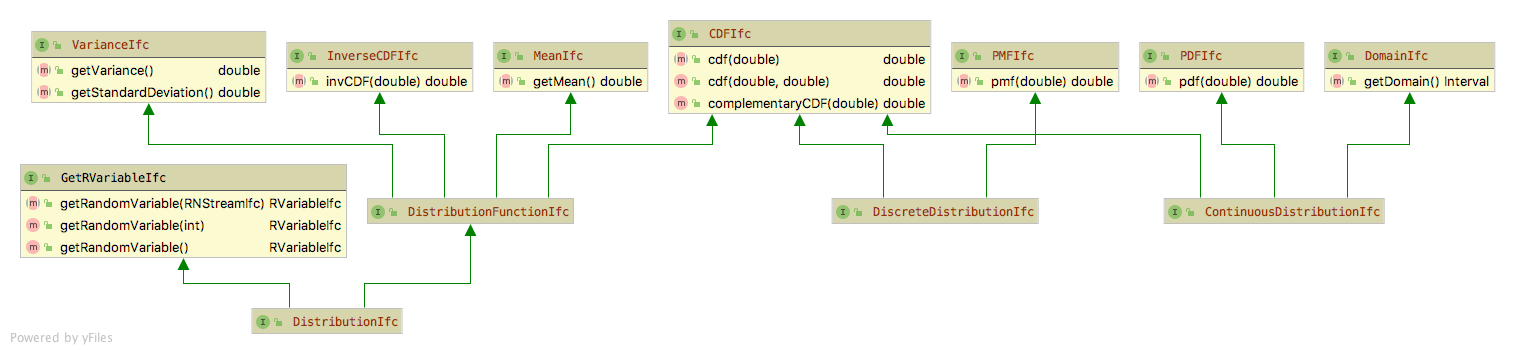
\includegraphics{./figures/Distributions.png}
\caption{\label{fig:DistPackage}Distribution Interfaces}
\end{figure}

Figure\ref{fig:DistPackage} illustrates the interfaces used to define probability distributions. First, the interface, \texttt{CDFIfc} serves as the basis for discrete distributions via the \texttt{DiscreteDistributionIfc} interface, for continuous distributions via the \texttt{ContinuousDistributionIfc} interface and the general \texttt{DistributionIfc} interface. The discrete distributions such as the geometric, binomial, etc. implement the \texttt{DiscreteDistributionIfc} and \texttt{PMFIfc} interfaces. Similarly, continuous distributions like the normal, uniform, etc. implement the \texttt{ContinuousDistributionIfc} and \texttt{PDFIfc} interfaces. All concrete implementations of distributions extend from the abstract base class \texttt{Distribution}, which implements the \texttt{DistributionIfc} interface. Thus, all distributions have the following capabilities:

\begin{itemize}
\tightlist
\item
  \texttt{cdf(double\ b)} - computes the cumulative probability, \(F(b) = P(X \leq b)\)
\item
  \texttt{cdf(double\ a,\ double\ b)} - computes the cumulative probability, \(P( a \leq X \leq b)\)
\item
  \texttt{complementaryCDF(double\ b)} - computes the cumulative probability, \(1-F(b) = P(X > b)\)
\item
  \texttt{getMean()} - returns the expected value (mean) of the distribution
\item
  \texttt{getVariance()} - returns the variance of the distribution
\item
  \texttt{getStandardDeviation()} - returns the standard deviation of the distribution
\item
  \texttt{invCDF(double\ p)} - returns the inverse of the cumulative distribution function \(F^{-1}(p)\). This is performed by numerical search if necessary
\end{itemize}

Discrete distributions have a method called \texttt{pmf(double\ k)} that returns the probability associated with the value \(k\). Continuous distributions have a probability density function, \(f(x)\), implemented in the method, \texttt{pdf(double\ x)}. Finally, all distributions know how to create random variables through the \texttt{GetRVariableIfc} interface that provides the following methods.

\begin{itemize}
\tightlist
\item
  \texttt{RVariableIfc\ getRandomVariable(RNStreamIfc\ stream)} - returns a new instance of a random variable based on the current values of the distribution's parameters that uses the supplied stream
\item
  \texttt{RVariableIfc\ getRandomVariable(int\ streamNum)} - returns a new instance of a random variable based on the current values of the distribution's parameters that uses the supplied stream number
\item
  \texttt{RVariableIfc\ getRandomVariable()} - returns a new instance of a random variable based on the current values of the distribution's parameters that uses a newly created stream
\end{itemize}

As an example, the following code illustrates some calculations for the binomial distribution.

\begin{Shaded}
\begin{Highlighting}[]
\CommentTok{// make and use a Binomial(p, n) distribution}
\DataTypeTok{int}\NormalTok{ n }\OperatorTok{=} \DecValTok{10}\OperatorTok{;}
\DataTypeTok{double}\NormalTok{ p }\OperatorTok{=} \FloatTok{0.8}\OperatorTok{;}
\BuiltInTok{System}\OperatorTok{.}\FunctionTok{out}\OperatorTok{.}\FunctionTok{println}\OperatorTok{(}\StringTok{"n = "} \OperatorTok{+}\NormalTok{ n}\OperatorTok{);}
\BuiltInTok{System}\OperatorTok{.}\FunctionTok{out}\OperatorTok{.}\FunctionTok{println}\OperatorTok{(}\StringTok{"p = "} \OperatorTok{+}\NormalTok{ p}\OperatorTok{);}
\NormalTok{Binomial bnDF }\OperatorTok{=} \KeywordTok{new} \FunctionTok{Binomial}\OperatorTok{(}\NormalTok{p}\OperatorTok{,}\NormalTok{ n}\OperatorTok{);}
\BuiltInTok{System}\OperatorTok{.}\FunctionTok{out}\OperatorTok{.}\FunctionTok{println}\OperatorTok{(}\StringTok{"mean = "} \OperatorTok{+}\NormalTok{ bnDF}\OperatorTok{.}\FunctionTok{getMean}\OperatorTok{());}
\BuiltInTok{System}\OperatorTok{.}\FunctionTok{out}\OperatorTok{.}\FunctionTok{println}\OperatorTok{(}\StringTok{"variance = "} \OperatorTok{+}\NormalTok{ bnDF}\OperatorTok{.}\FunctionTok{getVariance}\OperatorTok{());}
\CommentTok{// compute some values}
\BuiltInTok{System}\OperatorTok{.}\FunctionTok{out}\OperatorTok{.}\FunctionTok{printf}\OperatorTok{(}\StringTok{"}\SpecialCharTok{\%3s}\StringTok{ }\SpecialCharTok{\%15s}\StringTok{ }\SpecialCharTok{\%15s}\StringTok{ }\SpecialCharTok{\%n}\StringTok{"}\OperatorTok{,} \StringTok{"k"}\OperatorTok{,} \StringTok{"p(k)"}\OperatorTok{,} \StringTok{"cdf(k)"}\OperatorTok{);}
\ControlFlowTok{for} \OperatorTok{(}\DataTypeTok{int}\NormalTok{ i }\OperatorTok{=} \DecValTok{0}\OperatorTok{;}\NormalTok{ i }\OperatorTok{\textless{}=} \DecValTok{10}\OperatorTok{;}\NormalTok{ i}\OperatorTok{++)} \OperatorTok{\{}
    \BuiltInTok{System}\OperatorTok{.}\FunctionTok{out}\OperatorTok{.}\FunctionTok{printf}\OperatorTok{(}\StringTok{"}\SpecialCharTok{\%3d}\StringTok{ }\SpecialCharTok{\%15.10f}\StringTok{ }\SpecialCharTok{\%15.10f}\StringTok{ }\SpecialCharTok{\%n}\StringTok{"}\OperatorTok{,}\NormalTok{ i}\OperatorTok{,}\NormalTok{ bnDF}\OperatorTok{.}\FunctionTok{pmf}\OperatorTok{(}\NormalTok{i}\OperatorTok{),}\NormalTok{ bnDF}\OperatorTok{.}\FunctionTok{cdf}\OperatorTok{(}\NormalTok{i}\OperatorTok{));}
\OperatorTok{\}}
\end{Highlighting}
\end{Shaded}

The output shows the mean, variance, and basic probability calculations.

\begin{verbatim}
n = 10
p = 0.8
mean = 8.0
variance = 1.5999999999999996
  k            p(k)          cdf(k) 
  0    0.0000001024    0.0000001024 
  1    0.0000040960    0.0000041984 
  2    0.0000737280    0.0000779264 
  3    0.0007864320    0.0008643584 
  4    0.0055050240    0.0063693824 
  5    0.0264241152    0.0327934976 
  6    0.0880803840    0.1208738816 
  7    0.2013265920    0.3222004736 
  8    0.3019898880    0.6241903616 
  9    0.2684354560    0.8926258176 
 10    0.1073741824    1.0000000000 
\end{verbatim}

The \texttt{jsl.utilities.random.rvariable} package creates instances of random variables that are immutable. That is, once you create a random variable, its parameters cannot be changed. However, distributions permit their parameters to be changed and they also facilitate the creation of random variables. The following code uses the \texttt{setParameters()} method to change the parameters of the previously created binomial distribution and then creates a random variable based on the mutated distribution.

\begin{Shaded}
\begin{Highlighting}[]
\CommentTok{// change the probability and number of trials}
\NormalTok{bnDF}\OperatorTok{.}\FunctionTok{setParameters}\OperatorTok{(}\FloatTok{0.5}\OperatorTok{,} \DecValTok{20}\OperatorTok{);}
\BuiltInTok{System}\OperatorTok{.}\FunctionTok{out}\OperatorTok{.}\FunctionTok{println}\OperatorTok{(}\StringTok{"mean = "} \OperatorTok{+}\NormalTok{ bnDF}\OperatorTok{.}\FunctionTok{getMean}\OperatorTok{());}
\BuiltInTok{System}\OperatorTok{.}\FunctionTok{out}\OperatorTok{.}\FunctionTok{println}\OperatorTok{(}\StringTok{"variance = "} \OperatorTok{+}\NormalTok{ bnDF}\OperatorTok{.}\FunctionTok{getVariance}\OperatorTok{());}
\CommentTok{// make random variables based on the distributions}
\NormalTok{RVariableIfc brv }\OperatorTok{=}\NormalTok{ bnDF}\OperatorTok{.}\FunctionTok{getRandomVariable}\OperatorTok{();}
\BuiltInTok{System}\OperatorTok{.}\FunctionTok{out}\OperatorTok{.}\FunctionTok{printf}\OperatorTok{(}\StringTok{"}\SpecialCharTok{\%3s}\StringTok{ }\SpecialCharTok{\%15s}\StringTok{ }\SpecialCharTok{\%n}\StringTok{"}\OperatorTok{,} \StringTok{"n"}\OperatorTok{,} \StringTok{"Values"}\OperatorTok{);}
\CommentTok{// generate some values}
\ControlFlowTok{for} \OperatorTok{(}\DataTypeTok{int}\NormalTok{ i }\OperatorTok{=} \DecValTok{0}\OperatorTok{;}\NormalTok{ i }\OperatorTok{\textless{}} \DecValTok{5}\OperatorTok{;}\NormalTok{ i}\OperatorTok{++)} \OperatorTok{\{}
    \CommentTok{// getValue() method returns generated values}
    \DataTypeTok{int}\NormalTok{ x }\OperatorTok{=} \OperatorTok{(}\DataTypeTok{int}\OperatorTok{)}\NormalTok{brv}\OperatorTok{.}\FunctionTok{getValue}\OperatorTok{();}
    \BuiltInTok{System}\OperatorTok{.}\FunctionTok{out}\OperatorTok{.}\FunctionTok{printf}\OperatorTok{(}\StringTok{"}\SpecialCharTok{\%3d}\StringTok{ }\SpecialCharTok{\%15d}\StringTok{ }\SpecialCharTok{\%n}\StringTok{"}\OperatorTok{,}\NormalTok{ i}\OperatorTok{+}\DecValTok{1}\OperatorTok{,}\NormalTok{ x}\OperatorTok{);}
\OperatorTok{\}}
\end{Highlighting}
\end{Shaded}

The results are as we would expect. Similar calculations can be made for continuous distributions. In most cases, the concrete implementations of the various distributions have specialize methods beyond those generic methods described here. Please refer to the java docs for further details.

\begin{verbatim}
mean = 10.0
variance = 5.0
  n          Values 
  1              11 
  2              14 
  3              16 
  4               7 
  5              14 
\end{verbatim}

There are a number of useful static methods defined for the binomial, normal, gamma, and Student-T distributions. Specifically, for the binomial distribution, has the following static methods

\begin{itemize}
\tightlist
\item
  \texttt{binomialPMF(int\ j,\ int\ n,\ double\ p)} - directly computes the probability for the value \(j\)
\item
  \texttt{binomialCDF(int\ j,\ int\ n,\ double\ p)} - directly computes the cumulative distribution function for the value \(j\)
\item
  \texttt{binomialCCDF(int\ j,\ int\ n,\ double\ p)}- directly computes the complementary cumulative distribution function for the value of \(j\)
\item
  \texttt{binomialInvCDF(double\ x,\ int\ n,\ double\ p)} - directly computes the inverse cumulative distribution function
\end{itemize}

These methods are designed to perform their calculations in a numerically stable manner to ensure numerical accuracy. The normal distribution has the following static methods for computations involving the standard normal distribution.

\begin{itemize}
\tightlist
\item
  \texttt{stdNormalCDF(double\ z)} - the cumulative probability for a \(Z ~ N(0,1)\) random variable, i.e.~\(F(z) = P(Z \leq z)\)
\item
  \texttt{stdNormalComplementaryCDF(double\ z)} - returns \(1-P(Z \leq z)\)
\item
  \texttt{stdNormalInvCDF(double\ p)} - returns \$ z = F\^{}\{-1\}(p)\$ the inverse of the cumulative distribution function
\end{itemize}

The Student-T distribution also has two static convenience methods to facilitate computations.

\begin{itemize}
\tightlist
\item
  \texttt{getCDF(double\ dof,\ double\ x)} - computes the cumulative distribution function for \(x\) given the degrees of freedom
\item
  \texttt{getInvCDF(double\ dof,\ double\ p)} - computes the inverse cumulative distribution function or t-value for the supplied probability given the degrees of freedom.
\end{itemize}

Within the gamma distribution there are some convenience methods for computing the gamma function, the natural logarithm of the gamma function, the incomplete gamma function, and the digamma function (derivative of the natural logarithm of the gamma function).

\hypertarget{statistics}{%
\chapter{Collecting Statistics}\label{statistics}}

\textbf{\textsc{Learning Objectives}}

\begin{itemize}
\item
  To be able to collect statistics using classes within the JSL
\item
\begin{verbatim}
To understand the basics of statistical computations supported by the JSL
\end{verbatim}
\end{itemize}

The JSL has a wide variety of classes that support statistic computations. A main theme in understanding the usage of the classes within the \href{https://rossetti.git-pages.uark.edu/JSL-Documentation/jsl/utilities/statistic/package-summary.html}{\texttt{jsl.utilities.statistics}} package is the concept of collection. This concept is encapsulated within the interface, \texttt{CollectorIfc} interface. The methods of the \texttt{CollectorIfc} interface are illustrated in Figure \ref{fig:CollectorIfc}.

\begin{figure}
\centering
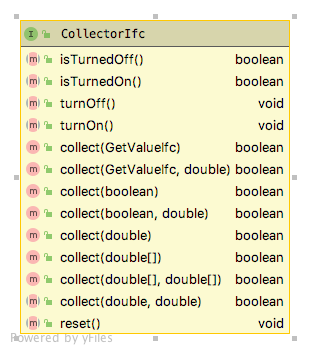
\includegraphics{./figures/CollectInterface.png}
\caption{\label{fig:CollectorIfc}CollectorIfc Interface}
\end{figure}

Something is a collector, if it implements the \texttt{CollectorIfc} interface. The implication is that those values presented to the various \texttt{collect} methods will be observed and tabulated into various quantities based on the presented values. The \texttt{collect} method has been overridden to facilitate collection of double values, arrays of double values, and boolean values. The two parameter \texttt{collect} methods permit collection of a second set of values. The second parameter is meant to represent the weight associated with the first parameter. As we will see, this facilitates the collection of weighted statistics. Collection can be turned on or off and can be reset. Turning collection off should cause the presented values to be ignored during the off period. Resetting a collector should set the state of the collector as if no values had been presented. Thus, resetting a collector should clear all previous collection results.

Figure \ref{fig:Statistics} presents the major classes and interfaces within the statistics package. The \texttt{CollectIfc} interface is implemented within the abstract base class \texttt{AbstractCollector}, which serves as the basis for various concrete implementations of statistical collectors. The \texttt{SaveDataIfc} interface defines methods for indicating whether or not the data collected should be saved into arrays. There are two major kinds of statistics one of which assumes that the values presented must be weighted, the \texttt{WeightedStatisticIfc} interface and the \texttt{WeightedStatistic} class. While the other branch of classes, derived from \texttt{AbstractStatistic} do not necessarily have to be weighted. The main classes to be discussed here are \texttt{Statistic} and \texttt{Histogram}.

\begin{figure}
\centering
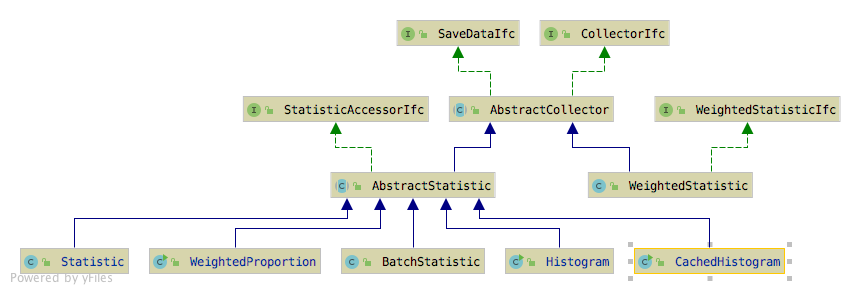
\includegraphics{./figures/Statistics.png}
\caption{\label{fig:Statistics}Major Classes and Interfaces in the Statistics Package}
\end{figure}

\hypertarget{creating-and-using-a-statistic}{%
\section{Creating and Using a Statistic}\label{creating-and-using-a-statistic}}

The \texttt{Statistic} class has a great deal of functionality. It accumulates summary statistics on the values presented to it via its \texttt{collect} methods. Recall also that since the \texttt{Statistic} class implements the \texttt{CollectorIfc} interface, you can use the \texttt{reset()} method to clear all accumulated statistics and reuse the \texttt{Statistic} instance. The major statistical quantities are found in the \texttt{StatisticAccessor} interface.

\begin{figure}

{\centering 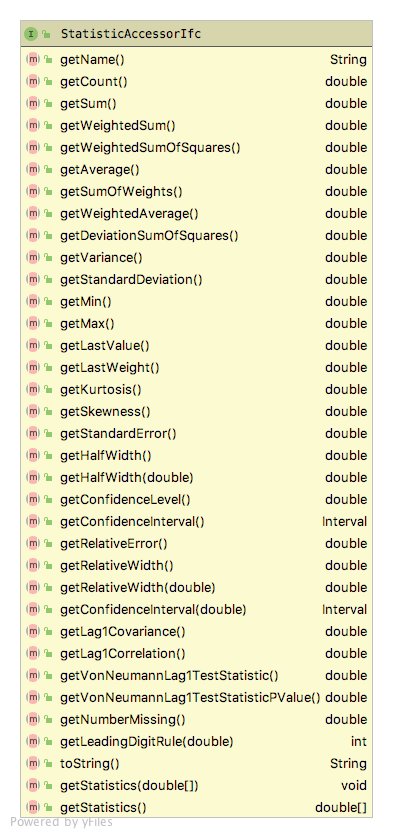
\includegraphics[width=0.6\linewidth,height=0.6\textheight]{./figures/StatisticAccessor} 

}

\caption{Major Accumulated Statistical Quantities}\label{fig:StatisticAccessor}
\end{figure}

As can be seen in Figure \ref{fig:StatisticAccessor}, the \texttt{Statistic} class not only computes the standard statistical quantities such as the count, average, and variance, it also has functionality to compute confidence intervals, skewness, kurtosis, the minimum, the maximum, and lag 1 covariance and correlation. The computed confidence intervals are based on the assumption that the observed data are normally distributed or that the sample size is large enough to justify using the central limit theorem to assume that the sampling distribution is normal. Thus, we can assume that the confidence intervals are approximate. The summary statistics are computed via efficient one pass algorithms that do not require any observed data to be stored. The algorithms are designed to minimize issues related to numerical precision within the calculated results. The \texttt{toString()} method of the \texttt{Statistic} class has been overridden to contain all of the computed values. Let's illustrate the usage of the \texttt{Statistic} class with some code. In this code, first we create a normal random variable to be able to generate some data. Then, two statistics are created. The first statistic directly collects the generated values. The second statistic is designed to collect \(P(X\geq 20.0)\) by observing whether or not the generated value meets this criteria as defined by the boolean expression \texttt{x\ \textgreater{}=\ 20.0}.

\begin{Shaded}
\begin{Highlighting}[]
\CommentTok{// create a normal mean = 20.0, variance = 4.0 random variable}
\NormalTok{NormalRV n }\OperatorTok{=} \KeywordTok{new} \FunctionTok{NormalRV}\OperatorTok{(}\FloatTok{20.0}\OperatorTok{,} \FloatTok{4.0}\OperatorTok{);}
\CommentTok{// create a Statistic to observe the values}
\NormalTok{Statistic stat }\OperatorTok{=} \KeywordTok{new} \FunctionTok{Statistic}\OperatorTok{(}\StringTok{"Normal Stats"}\OperatorTok{);}
\NormalTok{Statistic pGT20 }\OperatorTok{=} \KeywordTok{new} \FunctionTok{Statistic}\OperatorTok{(}\StringTok{"P(X\textgreater{}=20"}\OperatorTok{);}
\CommentTok{// generate 100 values}
\ControlFlowTok{for} \OperatorTok{(}\DataTypeTok{int}\NormalTok{ i }\OperatorTok{=} \DecValTok{1}\OperatorTok{;}\NormalTok{ i }\OperatorTok{\textless{}=} \DecValTok{100}\OperatorTok{;}\NormalTok{ i}\OperatorTok{++)} \OperatorTok{\{}
    \CommentTok{// getValue() method returns generated values}
    \DataTypeTok{double}\NormalTok{ x }\OperatorTok{=}\NormalTok{ n}\OperatorTok{.}\FunctionTok{getValue}\OperatorTok{();}
\NormalTok{    stat}\OperatorTok{.}\FunctionTok{collect}\OperatorTok{(}\NormalTok{x}\OperatorTok{);}
\NormalTok{    pGT20}\OperatorTok{.}\FunctionTok{collect}\OperatorTok{(}\NormalTok{x }\OperatorTok{\textgreater{}=} \FloatTok{20.0}\OperatorTok{);}
\OperatorTok{\}}
\BuiltInTok{System}\OperatorTok{.}\FunctionTok{out}\OperatorTok{.}\FunctionTok{println}\OperatorTok{(}\NormalTok{stat}\OperatorTok{);}
\end{Highlighting}
\end{Shaded}

The results for the statistics collected directly on the observations from the \texttt{toString()} method are as follows.

\begin{verbatim}
ID 1
Name Normal Stats
Number 100.0
Average 20.370190128861807
Standard Deviation 2.111292233346322
Standard Error 0.2111292233346322
Half-width 0.4189261806189412
Confidence Level 0.95
Confidence Interval [19.951263948242865, 20.78911630948075]
Minimum 15.020744984423821
Maximum 25.33588436770212
Sum 2037.0190128861807
Variance 4.457554894588499
Weighted Average 20.370190128861797
Weighted Sum 2037.0190128861796
Sum of Weights 100.0
Weighted Sum of Squares 41935.76252316213
Deviation Sum of Squares 441.2979345642614
Last value collected 21.110736402119805
Last weighted collected 1.0
Kurtosis -0.534855387072145
Skewness 0.20030433873223502
Lag 1 Covariance -0.973414579833684
Lag 1 Correlation -0.22057990840016864
Von Neumann Lag 1 Test Statistic -2.2136062395518343
Number of missing observations 0.0
Lead-Digit Rule(1) -1
\end{verbatim}

Of course, this is probably more output than what you need, but you can use the methods illustrated in Figure \ref{fig:StatisticAccessor} to access specific desired quantities. Notice that in the code example that the \(P(X \geq 20.0)\) is also collected. This is done by using the boolean expression \texttt{x\ \textgreater{}=\ 20.0} within the \texttt{collect()} method. This expression evaluates to either true or false. The true values are presented as 1.0 and the false values as 0.0. Thus, this expression acts as an indicator variable and facilitates the estimation of probabilities. The results from the statistics can be pretty printed by using the \texttt{StatisticReporter} class, which takes a list of objects that implement the \texttt{StatisticAccessorIfc} interface and facilitates the writing and printing of various statistical summary reports.

\begin{Shaded}
\begin{Highlighting}[]
\NormalTok{StatisticReporter reporter }\OperatorTok{=} \KeywordTok{new} \FunctionTok{StatisticReporter}\OperatorTok{(}\BuiltInTok{List}\OperatorTok{.}\FunctionTok{of}\OperatorTok{(}\NormalTok{stat}\OperatorTok{,}\NormalTok{ pGT20}\OperatorTok{));}
\BuiltInTok{System}\OperatorTok{.}\FunctionTok{out}\OperatorTok{.}\FunctionTok{println}\OperatorTok{(}\NormalTok{reporter}\OperatorTok{.}\FunctionTok{getHalfWidthSummaryReport}\OperatorTok{());}
\end{Highlighting}
\end{Shaded}

\begin{verbatim}
Half-Width Statistical Summary Report - Confidence Level (95.000)% 

Name                                                Count         Average      Half-Width 
---------------------------------------------------------------------------------------------------- 
Normal Stats                                          100         20.3702          0.4189 
P(X>=20                                               100          0.5100          0.0997 
---------------------------------------------------------------------------------------------------- 
\end{verbatim}

The \texttt{Statistic} class has a number of very useful static methods that work on arrays and compute various statistical quantities.

\begin{itemize}
\tightlist
\item
  \texttt{int\ getIndexOfMin(double{[}{]}\ x)} - returns the index of the element that is smallest. If there are ties, the first found is returned.
\item
  \texttt{double\ getMin(double{[}{]}\ x)} - returns the element that is smallest. If there are ties, the first found is returned.
\item
  \texttt{int\ getIndexOfMax(double{[}{]}\ x)} - returns the index of the element that is largest If there are ties, the first found is returned.
\item
  \texttt{double\ getMax(double{[}{]}\ x)} - returns the element that is largest. If there are ties, the first found is returned.
\item
  \texttt{double\ getMedian(double{[}{]}\ data)} - returns the value that has 50 percent of the data above and below it.
\item
  \texttt{int\ countLessEqualTo(double{[}{]}\ data,\ double\ x)} - returns the count of the elements that are less than or equal to \(x\)
\item
  \texttt{int\ countLessThan(double{[}{]}\ data,\ double\ x)} - returns the count of the elements that are less than \(x\)
\item
  \texttt{int\ countGreaterEqualTo(double{[}{]}\ data,\ double\ x)} - returns the count of the elements that are greater than or equal to \(x\)
\item
  \texttt{int\ countGreaterThan(double{[}{]}\ data,\ double\ x)} - returns the count of the elements that are greater than \(x\)
\item
  \texttt{double{[}{]}\ getOrderStatistics(double{[}{]}\ data)} - returns a sorted copy of the supplied array ordered from smallest to largest
\item
  long estimateSampleSize(double desiredHW, double stdDev, double level)` - returns the approximate sample size necessary to reach the desired half-width at the specified confidence level given the estimate of the sample standard deviation.
\item
  \texttt{Statistic\ collectStatistics(double{[}{]}\ x,\ double{[}{]}\ w)} - returns an instance of \texttt{Statistic} that summarizes the array of values and the supplied weights.
\item
  \texttt{collectStatistics(double{[}{]}\ x)} - returns an instance of \texttt{Statistic} that summarizes the array of values
\end{itemize}

\hypertarget{histograms-and-frequencies}{%
\section{Histograms and Frequencies}\label{histograms-and-frequencies}}

A histogram tabulates counts and frequencies of observed data over a set of contiguous intervals. Let \(b_{0}, b_{1}, \cdots, b_{k}\) be the breakpoints (end points) of the class intervals such that \(\left(b_{0}, b_{1} \right], \left(b_{1}, b_{2} \right], \cdots, \left(b_{k-1}, b_{k} \right]\) form \(k\) disjoint and adjacent intervals. The intervals do not have to be of equal width. Also, \(b_{0}\) can be equal to \(-\infty\) resulting in interval \(\left(-\infty, b_{1} \right]\) and \(b_{k}\) can be equal to \(+\infty\) resulting in interval \(\left(b_{k-1}, +\infty \right)\). Define \(\Delta b_j = b_{j} - b_{j-1}\) and if all the intervals have the same width (except perhaps for the end intervals), \(\Delta b = \Delta b_j\). To count the number of observations that fall in each interval, we can use the count function:
\[
c(\vec{x}\leq b) = \#\lbrace x_i \leq b \rbrace \; i=1,\ldots,n
\]
\(c(\vec{x}\leq b)\) counts the number of observations less than or equal to \(x\). Let \(c_{j}\) be the observed count of the \(x\) values contained in the \(j^{th}\) interval \(\left(b_{j-1}, b_{j} \right]\). Then, we can determine \(c_{j}\) via the following equation:
\[
c_{j} = c(\vec{x}\leq b_{j}) - c(\vec{x}\leq b_{j-1})
\]
The key parameters of a histogram are:

\begin{itemize}
\tightlist
\item
  The first bin lower limit (\(b_{0}\)): This is the starting point of the range over which the data will be tabulated.
\item
  The number of bins (\(k\)))
\item
  The width of the bins, (\(\Delta b\))
\end{itemize}

\begin{figure}

{\centering 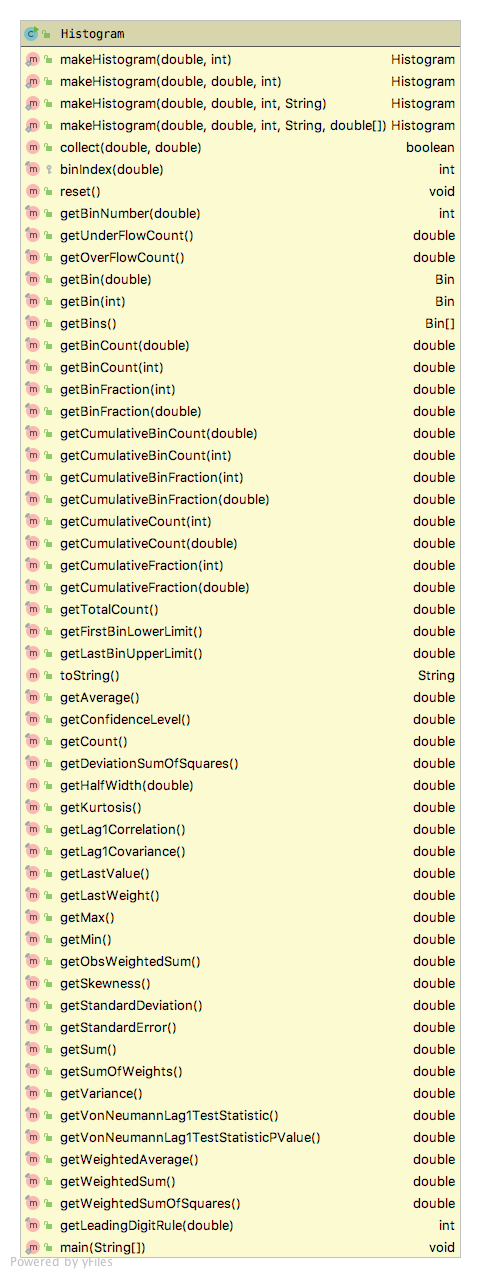
\includegraphics[width=0.6\linewidth,height=0.6\textheight]{./figures/Histogram} 

}

\caption{Histogram Class}\label{fig:Histogram}
\end{figure}

Figure \ref{fig:Histogram} presents the methods of the \texttt{Histogram} class. The \texttt{Histogram} class is utilized in a very similar manner as the \texttt{Statistic} class by collecting observations. The observations are then tabulated into the bins. The \texttt{Histogram} class allows the user to tabulate the bin contents via the collect() methods inherited from the \texttt{AbstractStatistic} base class. Since data may fall below the first bin and after the last bin, the implementation also provides counts for those occurrences. Since a \texttt{Histogram} is a sub-class of \texttt{AbstractStatistic}, it also implements the \texttt{StatisticAccessorIfc} to provide summary statistics on the data tabulated within the bins. The \texttt{Histogram} class also provides static methods to create histograms based on a range (lower limit to upper limit) with a given number of bins. In this case, an appropriate bin width is computed.

In some cases, the client may not know in advance the appropriate settings for the number of bins or the width of the bins. In this situation, one can use the \texttt{CachedHistogram} class, which first collects the data in a temporary cache array. Once the cache has been filled up, the \texttt{CachedHistogram} computes a reasonable lower limit, number of bins, and bin width based on the statistics collected over the cache. The underlying histogram is available via the getHistogram() method after the cache has been used.

\begin{Shaded}
\begin{Highlighting}[]
\NormalTok{ExponentialRV d }\OperatorTok{=} \KeywordTok{new} \FunctionTok{ExponentialRV}\OperatorTok{(}\DecValTok{2}\OperatorTok{);}
\CommentTok{// create a histogram with lower limit 0.0, 20 bins, of width 0.1}
\NormalTok{Histogram h }\OperatorTok{=} \KeywordTok{new} \FunctionTok{Histogram}\OperatorTok{(}\FloatTok{0.0}\OperatorTok{,} \DecValTok{20}\OperatorTok{,} \FloatTok{0.1}\OperatorTok{);}
\ControlFlowTok{for} \OperatorTok{(}\DataTypeTok{int}\NormalTok{ i }\OperatorTok{=} \DecValTok{1}\OperatorTok{;}\NormalTok{ i }\OperatorTok{\textless{}=} \DecValTok{100}\OperatorTok{;} \OperatorTok{++}\NormalTok{i}\OperatorTok{)} \OperatorTok{\{}
\NormalTok{    h}\OperatorTok{.}\FunctionTok{collect}\OperatorTok{(}\NormalTok{d}\OperatorTok{.}\FunctionTok{getValue}\OperatorTok{());}
\OperatorTok{\}}
\BuiltInTok{System}\OperatorTok{.}\FunctionTok{out}\OperatorTok{.}\FunctionTok{println}\OperatorTok{(}\NormalTok{h}\OperatorTok{);}
\end{Highlighting}
\end{Shaded}

\begin{verbatim}
Histogram: Histogram
-------------------------------------
Number of bins = 20
Bin width = 0.1
First bin starts at = 0.0
Last bin ends at = 2.0
Under flow count = 0.0
Over flow count = 45.0
Total bin count = 55.0
Total count = 100.0
-------------------------------------
Bin Range        Count Total Prob  CumProb
  1 [0.00,0.10)   2.0   2.0 0.036364 0.036364 
  2 [0.10,0.20)   5.0   7.0 0.090909 0.127273 
  3 [0.20,0.30)   5.0  12.0 0.090909 0.218182 
  4 [0.30,0.40)   2.0  14.0 0.036364 0.254545 
  5 [0.40,0.50)   7.0  21.0 0.127273 0.381818 
  6 [0.50,0.60)   3.0  24.0 0.054545 0.436364 
  7 [0.60,0.70)   3.0  27.0 0.054545 0.490909 
  8 [0.70,0.80)   3.0  30.0 0.054545 0.545455 
  9 [0.80,0.90)   2.0  32.0 0.036364 0.581818 
 10 [0.90,1.00)   2.0  34.0 0.036364 0.618182 
 11 [1.00,1.10)   5.0  39.0 0.090909 0.709091 
 12 [1.10,1.20)   6.0  45.0 0.109091 0.818182 
 13 [1.20,1.30)   2.0  47.0 0.036364 0.854545 
 14 [1.30,1.40)   2.0  49.0 0.036364 0.890909 
 15 [1.40,1.50)   3.0  52.0 0.054545 0.945455 
 16 [1.50,1.60)   1.0  53.0 0.018182 0.963636 
 17 [1.60,1.70)   1.0  54.0 0.018182 0.981818 
 18 [1.70,1.80)   1.0  55.0 0.018182 1.000000 
 19 [1.80,1.90)   0.0  55.0 0.000000 1.000000 
 20 [1.90,2.00)   0.0  55.0 0.000000 1.000000 
\end{verbatim}

The JSL will also tabulate count frequencies when the values are only integers. This is accomplished with the \texttt{IntegerFrequency} class. Figure \ref{fig:Frequency} indicates the methods of the \texttt{IntegerFrequency} class. The object can return information on the counts and proportions. It can even create a \texttt{DEmpiricalCDF} distribution based on the observed data.

\begin{figure}
\centering
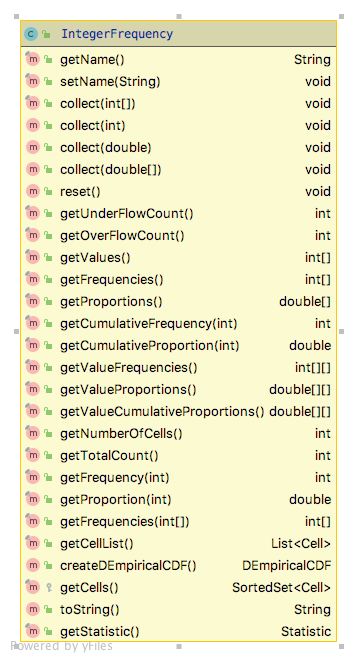
\includegraphics{./figures/Frequency.png}
\caption{\label{fig:Frequency}IntegerFrequence Class}
\end{figure}

In the following code example, an instance of the \texttt{IntegerFrequency} class is created. Then, an instance of a binomial random variable is used to generate a sample of 10,000 observations. The sample is then collected by the \texttt{IntegerFrequency} class's \texttt{collect()} method.

\begin{Shaded}
\begin{Highlighting}[]
\NormalTok{IntegerFrequency f }\OperatorTok{=} \KeywordTok{new} \FunctionTok{IntegerFrequency}\OperatorTok{(}\StringTok{"Frequency Demo"}\OperatorTok{);}
\NormalTok{BinomialRV bn }\OperatorTok{=} \KeywordTok{new} \FunctionTok{BinomialRV}\OperatorTok{(}\FloatTok{0.5}\OperatorTok{,} \DecValTok{100}\OperatorTok{);}
\DataTypeTok{double}\OperatorTok{[]}\NormalTok{ sample }\OperatorTok{=}\NormalTok{ bn}\OperatorTok{.}\FunctionTok{sample}\OperatorTok{(}\DecValTok{10000}\OperatorTok{);}
\NormalTok{f}\OperatorTok{.}\FunctionTok{collect}\OperatorTok{(}\NormalTok{sample}\OperatorTok{);}
\BuiltInTok{System}\OperatorTok{.}\FunctionTok{out}\OperatorTok{.}\FunctionTok{println}\OperatorTok{(}\NormalTok{f}\OperatorTok{);}
\end{Highlighting}
\end{Shaded}

As can be noted in the output, only those integers that are actually observed are tabulated in terms of the count of the number of times the integer is observed and its proportion. The user does not have to specify the range of possible integers; however, instances of \texttt{IntegerFrequency} can be created that specify a lower and upper limit on the tabulated values. The overflow and underflow counts then tabulate when observations fall outside of the specified range.

\begin{verbatim}
Frequency Tabulation Frequency Demo
----------------------------------------
Number of cells = 39
Lower limit = -2147483648
Upper limit = 2147483647
Under flow count = 0
Over flow count = 0
Total count = 10000
----------------------------------------
Value    Count   Proportion
31   1   1.0E-4
33   4   4.0E-4
34   5   5.0E-4
35   9   9.0E-4
36   17      0.0017
37   28      0.0028
38   41      0.0041
39   74      0.0074
40   100     0.01
41   192     0.0192
42   236     0.0236
43   277     0.0277
44   406     0.0406
45   453     0.0453
46   564     0.0564
47   653     0.0653
48   741     0.0741
49   762     0.0762
50   750     0.075
51   768     0.0768
52   783     0.0783
53   679     0.0679
54   600     0.06
55   484     0.0484
56   407     0.0407
57   324     0.0324
58   210     0.021
59   155     0.0155
60   108     0.0108
61   74      0.0074
62   41      0.0041
63   15      0.0015
64   15      0.0015
65   17      0.0017
66   3   3.0E-4
67   1   1.0E-4
69   1   1.0E-4
70   1   1.0E-4
71   1   1.0E-4
----------------------------------------
\end{verbatim}

Finally, the JSL provides the ability to define labeled states and to tabulate frequencies and proportions related to the visitation and transition between the states. This functionality is available in the \texttt{StateFrequency} class. The following code example creates an instance of \texttt{StateFrequency} by providing the number of states. The states are returned in a \texttt{List} and then 10,000 states are randomly selected from the list with equal probability using the \texttt{JSLRandom} functionality to randomly select from lists. The randomly selected state is then observed via the \texttt{collect()} method.

\begin{Shaded}
\begin{Highlighting}[]
\CommentTok{// number of states is 6}
\NormalTok{StateFrequency sf }\OperatorTok{=} \KeywordTok{new} \FunctionTok{StateFrequency}\OperatorTok{(}\DecValTok{6}\OperatorTok{);}
\BuiltInTok{List}\OperatorTok{\textless{}}\BuiltInTok{State}\OperatorTok{\textgreater{}}\NormalTok{ states }\OperatorTok{=}\NormalTok{ sf}\OperatorTok{.}\FunctionTok{getStates}\OperatorTok{();}
\ControlFlowTok{for}\OperatorTok{(}\DataTypeTok{int}\NormalTok{ i}\OperatorTok{=}\DecValTok{1}\OperatorTok{;}\NormalTok{i}\OperatorTok{\textless{}=}\DecValTok{10000}\OperatorTok{;}\NormalTok{i}\OperatorTok{++)\{}
    \BuiltInTok{State}\NormalTok{ state }\OperatorTok{=}\NormalTok{ JSLRandom}\OperatorTok{.}\FunctionTok{randomlySelect}\OperatorTok{(}\NormalTok{states}\OperatorTok{);}
\NormalTok{    sf}\OperatorTok{.}\FunctionTok{collect}\OperatorTok{(}\NormalTok{state}\OperatorTok{);}
\OperatorTok{\}}
\BuiltInTok{System}\OperatorTok{.}\FunctionTok{out}\OperatorTok{.}\FunctionTok{println}\OperatorTok{(}\NormalTok{sf}\OperatorTok{);}
\end{Highlighting}
\end{Shaded}

The output is what you would expect based on selecting the states with equal probability. Notice that the \texttt{StateFrequency} class not only tabulates the visits to the states, similar to \texttt{IntegerFrequency}, it also counts and tabulates the transitions between states. These detailed tabulations are available via the various methods of the class. See the Java docs for further details.

\begin{verbatim}
State Frequency Tabulation for: Identity#1
State Labels
State{id=1, number=0, name='State:0'}
State{id=2, number=1, name='State:1'}
State{id=3, number=2, name='State:2'}
State{id=4, number=3, name='State:3'}
State{id=5, number=4, name='State:4'}
State{id=6, number=5, name='State:5'}
State transition counts
[288, 272, 264, 282, 265, 286]
[283, 278, 283, 286, 296, 266]
[286, 298, 263, 264, 247, 282]
[271, 263, 275, 279, 280, 294]
[274, 305, 273, 281, 296, 268]
[254, 277, 282, 270, 313, 255]
State transition proportions
[0.17380808690404345, 0.16415208207604104, 0.15932407966203982, 0.17018708509354255, 0.15992757996378998, 0.17260108630054316]
[0.16725768321513002, 0.16430260047281323, 0.16725768321513002, 0.1690307328605201, 0.17494089834515367, 0.15721040189125296]
[0.174390243902439, 0.18170731707317073, 0.1603658536585366, 0.16097560975609757, 0.15060975609756097, 0.1719512195121951]
[0.16305655836341756, 0.1582430806257521, 0.1654632972322503, 0.16787003610108303, 0.1684717208182912, 0.17689530685920576]
[0.1614614024749558, 0.17972893341190335, 0.16087212728344136, 0.16558632881555688, 0.17442545668827342, 0.15792575132586917]
[0.15384615384615385, 0.16777710478497881, 0.17080557238037553, 0.16353725015142337, 0.18958207147183526, 0.15445184736523318]

Frequency Tabulation Identity#1
----------------------------------------
Number of cells = 6
Lower limit = 0
Upper limit = 5
Under flow count = 0
Over flow count = 0
Total count = 10000
----------------------------------------
Value    Count   Proportion
0    1657    0.1657
1    1693    0.1693
2    1640    0.164
3    1662    0.1662
4    1697    0.1697
5    1651    0.1651
----------------------------------------
\end{verbatim}

\hypertarget{batch-statistics}{%
\section{Batch Statistics}\label{batch-statistics}}

In simulation, we often collect data that is correlated, that is not independent. This causes difficulty in developing valid confidence intervals for the estimators. Grouping the data into batches and computing the average of each batch is one methodology for reducing the dependence within the data. The idea is that the average associated with each batch will tend to be less dependent, especially the larger the batch size. The method of batch means provides a mechanism for developing an estimator for \(Var\lbrack \bar{X} \rbrack\).

The method of batch means is based on observations \((X_{1}, X_{2}, X_{3}, \dots, X_{n})\). The idea is to group the output into batches of size, \(b\), such that the averages of the data within a batch are more nearly independent and possibly normally distributed.

\begin{multline*}
\underbrace{X_1, X_2, \ldots, X_b}_{batch 1} \cdots 
\underbrace{X_{b+1}, X_{b+2}, \ldots, X_{2b}}_{batch 2} \cdots \\
\underbrace{X_{(j-1)b+1}, X_{(j-1)b+2}, \ldots, X_{jb}}_{batch j}  \cdots 
\underbrace{X_{(k-1)b+1}, X_{(k-1)b+2}, \ldots, X_{kb}}_{batch k}
\end{multline*}

Let \(k\) be the number of batches each of size \(b\), where, \(b = \lfloor \frac{n}{k}\rfloor\). Define the \(j^{th}\) batch mean (average) as:

\[
\bar{X}_j(b) = \dfrac{1}{b} \sum_{i=1}^b X_{(j-1)b+i}
\]
Each of the batch means are treated like observations in the batch means series. For example, if the batch means are re-labeled as \(Y_j = \bar{X}_j(b)\), the batching process simply produces another series of data, (\(Y_1, Y_2, Y_3, \ldots, Y_k\)) which may be more like a random sample. Why should they be more independent? Typically, in auto-correlated processes the lag-k auto-correlations decay rapidly as \(k\) increases. Since, the batch means are formed from batches of size \(b\), provided that \(b\) is large enough the data within a batch is \emph{conceptually} far from the data in other batches. Thus, larger batch sizes are good for ensuring independence; however, as the batch size increases the number of batches decreases and thus variance of the estimator will increase.

To form a \((1 - \alpha)\)\% confidence interval, we simply treat this new series like a random sample and compute approximate confidence intervals using the sample average and sample variance of the batch means series:

\[
\bar{Y}(k) = \dfrac{1}{k} \sum_{j=1}^k Y_j
\]
The sample variance of the batch process is based on the \(k\) batches:
\[
S_b^2 (k) = \dfrac{1}{k - 1} \sum_{j=1}^k (Y_j - \bar{Y}^2)
\]
Finally, if the batch process can be considered independent and identically distributed the \(1-\alpha\) level confidence interval can be written as follows:
\[
\bar{Y}(k) \pm t_{\alpha/2, k-1} \dfrac{S_b (k)}{\sqrt{k}}
\]
The \texttt{BatchStatistic} class within the statistic package implements a basic batching process. The \texttt{BatchStatistic} class works with data as it is presented to its collect method. Since we do not know in advance how much data we have, the \texttt{BatchStatistic} class has rules about the minimum number of batches and the size of batches that can be formed. Theory indicates that we do not need to have a large number of batches and that it is better to have a relatively small number of batches that are large in size.

Three attributes of the BatchStatistic class that are important are:

\begin{itemize}
\tightlist
\item
  \texttt{myMinNumBatches} -- This represents the minimum number of batches required. The default value for this attribute is determined by \texttt{BatchStatistic}. \texttt{MIN\_NUM\_BATCHES}, which is set to 20.
\item
  \texttt{myMinBatchSize} -- This represents the minimum size for forming initial batches. The default value for this attribute is determined by \texttt{BatchStatistic}. \texttt{MIN\_NUM\_OBS\_PER\_BATCH}, which is set to 16.
\item
  \texttt{myMaxNumBatchesMultiple} -- This represents a multiple of minimum number of batches which is used to determine the upper limit (maximum) number of batches. For example, if \texttt{myMaxNumBatchesMultiple\ =\ 2} and the \texttt{myMinNumBatches\ =\ 20}, then the maximum number of batches we can have is 40 (2*20). The default value for this attribute is determined by \texttt{BatchStatistic}. \texttt{MAX\_BATCH\_MULTIPLE}, which is set to 2.
\end{itemize}

The \texttt{BatchStatistic} class uses instances of the \texttt{Statistic} class to do its calculations. The bulk of the processing is done in two methods, \texttt{collect()} and \texttt{collectBatch()}. The \texttt{collect()} method simply uses an instance of the \texttt{Statistic} class (\texttt{myStatistic}) to collect statistics. When the amount of data collected (\texttt{myStatistic.getCount()}) equals the current batch size (\texttt{myCurrentBatchSize}) then the \texttt{collectBatch()} method is called to form a batch.

\begin{Shaded}
\begin{Highlighting}[]
\KeywordTok{public} \DataTypeTok{final} \DataTypeTok{boolean} \FunctionTok{collect}\OperatorTok{(}\DataTypeTok{double}\NormalTok{ value}\OperatorTok{,} \DataTypeTok{double}\NormalTok{ weight}\OperatorTok{)} \OperatorTok{\{}
\CommentTok{// other code}
\NormalTok{myTotNumObs }\OperatorTok{=}\NormalTok{ myTotNumObs }\OperatorTok{+} \FloatTok{1.0}\OperatorTok{;}
\NormalTok{myValue }\OperatorTok{=}\NormalTok{ value}\OperatorTok{;}
\NormalTok{myWeight }\OperatorTok{=}\NormalTok{ weight}\OperatorTok{;}
\NormalTok{myStatistic}\OperatorTok{.}\FunctionTok{collect}\OperatorTok{(}\NormalTok{myValue}\OperatorTok{,}\NormalTok{ myWeight}\OperatorTok{);}
\ControlFlowTok{if} \OperatorTok{(}\NormalTok{myStatistic}\OperatorTok{.}\FunctionTok{getCount}\OperatorTok{()} \OperatorTok{==}\NormalTok{ myCurrentBatchSize}\OperatorTok{)} \OperatorTok{\{}
\NormalTok{   b }\OperatorTok{=} \FunctionTok{collectBatch}\OperatorTok{();}
\OperatorTok{\}}
\end{Highlighting}
\end{Shaded}

Referring to the collectBatch() method in the following code, the batches that are formed are recorded in an array called bm{[}{]}. After recording the batch average, the statistic is reset for collecting the next batch of data. The number of batches is recorded and if this has reached the maximum number of batches (as determined by the batch multiple calculation), we rebatch the batches back down to the minimum number of batches by combining adjacent batches according to the batch multiple.

\begin{Shaded}
\begin{Highlighting}[]
\KeywordTok{private} \DataTypeTok{boolean} \FunctionTok{collectBatch}\OperatorTok{()} \OperatorTok{\{}
    \DataTypeTok{boolean}\NormalTok{ b }\OperatorTok{=} \KeywordTok{true}\OperatorTok{;}
    \CommentTok{// increment the current number of batches}
\NormalTok{    myNumBatches }\OperatorTok{=}\NormalTok{ myNumBatches }\OperatorTok{+} \DecValTok{1}\OperatorTok{;}
    \CommentTok{// record the average of the batch}
\NormalTok{    bm}\OperatorTok{[}\NormalTok{myNumBatches}\OperatorTok{]} \OperatorTok{=}\NormalTok{ myStatistic}\OperatorTok{.}\FunctionTok{getWeightedAverage}\OperatorTok{();}
    \CommentTok{// collect running statistics on the batches}
\NormalTok{    b }\OperatorTok{=}\NormalTok{ myBMStatistic}\OperatorTok{.}\FunctionTok{collect}\OperatorTok{(}\NormalTok{bm}\OperatorTok{[}\NormalTok{myNumBatches}\OperatorTok{]);}
    \CommentTok{// reset the within batch statistic for next batch}
\NormalTok{    myStatistic}\OperatorTok{.}\FunctionTok{reset}\OperatorTok{();}
    \CommentTok{// if the number of batches has reached the maximum then rebatch down to}
    \CommentTok{// min number of batches}
    \ControlFlowTok{if} \OperatorTok{(}\NormalTok{myNumBatches }\OperatorTok{==}\NormalTok{ myMaxNumBatches}\OperatorTok{)} \OperatorTok{\{}
\NormalTok{        myNumRebatches}\OperatorTok{++;}
\NormalTok{        myCurrentBatchSize }\OperatorTok{=}\NormalTok{ myCurrentBatchSize }\OperatorTok{*}\NormalTok{ myMaxNumBatchesMultiple}\OperatorTok{;}
        \DataTypeTok{int}\NormalTok{ j }\OperatorTok{=} \DecValTok{0}\OperatorTok{;} \CommentTok{// within batch counter}
        \DataTypeTok{int}\NormalTok{ k }\OperatorTok{=} \DecValTok{0}\OperatorTok{;} \CommentTok{// batch counter}
\NormalTok{        myBMStatistic}\OperatorTok{.}\FunctionTok{reset}\OperatorTok{();} \CommentTok{// clear for collection across new batches}
        \CommentTok{// loop through all the batches}
        \ControlFlowTok{for} \OperatorTok{(}\DataTypeTok{int}\NormalTok{ i }\OperatorTok{=} \DecValTok{1}\OperatorTok{;}\NormalTok{ i }\OperatorTok{\textless{}=}\NormalTok{ myNumBatches}\OperatorTok{;}\NormalTok{ i}\OperatorTok{++)} \OperatorTok{\{}
\NormalTok{            myStatistic}\OperatorTok{.}\FunctionTok{collect}\OperatorTok{(}\NormalTok{bm}\OperatorTok{[}\NormalTok{i}\OperatorTok{]);} \CommentTok{// collect across batches old batches}
\NormalTok{            j}\OperatorTok{++;}
            \ControlFlowTok{if} \OperatorTok{(}\NormalTok{j }\OperatorTok{==}\NormalTok{ myMaxNumBatchesMultiple}\OperatorTok{)} \OperatorTok{\{} \CommentTok{// have enough for a batch}
                \CommentTok{//collect new batch average}
\NormalTok{                b }\OperatorTok{=}\NormalTok{ myBMStatistic}\OperatorTok{.}\FunctionTok{collect}\OperatorTok{(}\NormalTok{myStatistic}\OperatorTok{.}\FunctionTok{getAverage}\OperatorTok{());}
\NormalTok{                k}\OperatorTok{++;} \CommentTok{//count the batches}
\NormalTok{                bm}\OperatorTok{[}\NormalTok{k}\OperatorTok{]} \OperatorTok{=}\NormalTok{ myStatistic}\OperatorTok{.}\FunctionTok{getAverage}\OperatorTok{();} \CommentTok{// save the new batch average}
\NormalTok{                myStatistic}\OperatorTok{.}\FunctionTok{reset}\OperatorTok{();} \CommentTok{// reset for next batch}
\NormalTok{                j }\OperatorTok{=} \DecValTok{0}\OperatorTok{;}
            \OperatorTok{\}}
        \OperatorTok{\}}
\NormalTok{        myNumBatches }\OperatorTok{=}\NormalTok{ k}\OperatorTok{;} \CommentTok{// k should be minNumBatches}
\NormalTok{        myStatistic}\OperatorTok{.}\FunctionTok{reset}\OperatorTok{();} \CommentTok{//reset for use with new data}
    \OperatorTok{\}}
    \ControlFlowTok{return}\NormalTok{ b}\OperatorTok{;}
\OperatorTok{\}}
\end{Highlighting}
\end{Shaded}

There are a variety of procedures that have been developed that will automatically batch the data as it is collected. The JSL has a batching algorithm based on the procedure implemented within the Arena simulatin language. When a sufficient amount of data has been collected batches are formed. As more data is collected, additional batches are formed until \(k=40\) batches are collected. When 40 batches are formed, the algorithm collapses the number of batches back to 20, by averaging each pair of batches. This has the net effect of doubling the batch size. This process is repeated as more data is collected, thereby ensuring that the number of batches is between 20 and 39. In addition, the procedure also computes the lag-1 correlation so that independence of the batches can be tested.

The \texttt{BatchStatistic} class also provides a public \texttt{rebatchToNumberOfBatches()} method to allow the user to rebatch the batches to a user supplied number of batches. Since the \texttt{BatchStatistic} class implements the \texttt{StatisticalAccessorIfc} interface, it can return the sample average, sample variance, minimum, maximum, etc. of the batches. Within the discrete-event modeling constructs of the JSL, batching can be turned on to collect batch statistics during a replication. The use of these constructs will be discussed when the discrete-event modeling elements of the JSL are presented.

The following code illustrates how to create and use a \texttt{BatchStatistic}.

\begin{Shaded}
\begin{Highlighting}[]
\NormalTok{ExponentialRV d }\OperatorTok{=} \KeywordTok{new} \FunctionTok{ExponentialRV}\OperatorTok{(}\DecValTok{2}\OperatorTok{);}
\CommentTok{// number of observations}
\DataTypeTok{int}\NormalTok{ n }\OperatorTok{=} \DecValTok{1000}\OperatorTok{;} 
\CommentTok{// minimum number of batches permitted}
\CommentTok{// there will not be less than this number of batches}
\DataTypeTok{int}\NormalTok{ minNumBatches }\OperatorTok{=} \DecValTok{40}\OperatorTok{;}
\CommentTok{// minimum batch size permitted}
\CommentTok{// the batch size can be no smaller than this amount}
\DataTypeTok{int}\NormalTok{ minBatchSize }\OperatorTok{=} \DecValTok{25}\OperatorTok{;} 
\CommentTok{// maximum number of batch multiple}
\CommentTok{//  The multiple of the minimum number of batches}
\CommentTok{//  that determines the maximum number of batches}
\CommentTok{//  e.g. if the min. number of batches is 20}
\CommentTok{//  and the max number batches multiple is 2,}
\CommentTok{//  then we can have at most 40 batches}
\DataTypeTok{int}\NormalTok{ maxNBMultiple }\OperatorTok{=} \DecValTok{2}\OperatorTok{;} 
\CommentTok{// In this example, since 40*25 = 1000, the batch multiple does not matter}
\NormalTok{BatchStatistic bm }\OperatorTok{=} \KeywordTok{new} \FunctionTok{BatchStatistic}\OperatorTok{(}\NormalTok{minNumBatches}\OperatorTok{,}\NormalTok{ minBatchSize}\OperatorTok{,}\NormalTok{ maxNBMultiple}\OperatorTok{);}
\ControlFlowTok{for} \OperatorTok{(}\DataTypeTok{int}\NormalTok{ i }\OperatorTok{=} \DecValTok{1}\OperatorTok{;}\NormalTok{ i }\OperatorTok{\textless{}=}\NormalTok{ n}\OperatorTok{;} \OperatorTok{++}\NormalTok{i}\OperatorTok{)} \OperatorTok{\{}
\NormalTok{    bm}\OperatorTok{.}\FunctionTok{collect}\OperatorTok{(}\NormalTok{d}\OperatorTok{.}\FunctionTok{getValue}\OperatorTok{());}
\OperatorTok{\}}
\BuiltInTok{System}\OperatorTok{.}\FunctionTok{out}\OperatorTok{.}\FunctionTok{println}\OperatorTok{(}\NormalTok{bm}\OperatorTok{);}
\DataTypeTok{double}\OperatorTok{[]}\NormalTok{ bma }\OperatorTok{=}\NormalTok{ bm}\OperatorTok{.}\FunctionTok{getBatchMeanArrayCopy}\OperatorTok{();}
\DataTypeTok{int}\NormalTok{ i}\OperatorTok{=}\DecValTok{0}\OperatorTok{;}
\ControlFlowTok{for}\OperatorTok{(}\DataTypeTok{double}\NormalTok{ x}\OperatorTok{:}\NormalTok{ bma}\OperatorTok{)\{}
    \BuiltInTok{System}\OperatorTok{.}\FunctionTok{out}\OperatorTok{.}\FunctionTok{println}\OperatorTok{(}\StringTok{"bm("} \OperatorTok{+}\NormalTok{ i }\OperatorTok{+} \StringTok{") = "} \OperatorTok{+}\NormalTok{ x}\OperatorTok{);}
\NormalTok{    i}\OperatorTok{++;}
\OperatorTok{\}}
\CommentTok{// this rebatches the 40 down to 10}
\NormalTok{Statistic s }\OperatorTok{=}\NormalTok{ bm}\OperatorTok{.}\FunctionTok{rebatchToNumberOfBatches}\OperatorTok{(}\DecValTok{10}\OperatorTok{);}
\BuiltInTok{System}\OperatorTok{.}\FunctionTok{out}\OperatorTok{.}\FunctionTok{println}\OperatorTok{(}\NormalTok{s}\OperatorTok{);}
\end{Highlighting}
\end{Shaded}

\hypertarget{summary}{%
\section{Summary}\label{summary}}

The \texttt{jsl.utilities.statistic} package defines a lot of functionality. Here is a summary of some of the useful classes and interfaces.

\begin{enumerate}
\def\labelenumi{\arabic{enumi}.}
\tightlist
\item
  \texttt{CollectorIfc} defines a set of collect() methods for collecting data. The method is overridden to permit the collection of a wide variety of data type. The collect() method is designed to collect values and a weight associated with the value. This allows the collection of weighted statistics. \texttt{AbstractCollector} is an abstract base class for building concrete sub-classes.
\item
  \texttt{SaveDataIfc} defines methods for saving the observed data to arrays.
\item
  \texttt{WeightedStatisticIfc} defines statistics that are computed on weighted data values.
  \texttt{WeightedStatistic} is a concrete implementation of the interface.
\item
  \texttt{AbstractStatistic} is an abstract base class for defining statistics. Sub-classes of \texttt{AbstractStatistic} compute summary statistics of some kind.
\item
  \texttt{Histogram} defines a class to collect statistics and tabulate data into bins.
\item
  \texttt{Statistic} is a concrete implementation of \texttt{AbstractStatistic} allowing for a multitude of
  summary statistics.
\item
  \texttt{BatchStatistic} is also a concrete implementation of \texttt{AbstractStatistic} that provides for
  summarizing data via a batching process.
\item
  \texttt{IntegerFrequency} tabulates integer values into a frequencies by observed values, similar to a histogram.
\item
  \texttt{StateFrequency} facilitates defining labeled states and tabulating visitation and transition statistics.
\item
  \texttt{StatisticXY} collects statistics on \((x,y)\) pairs computing statistics on the \(x\) and \(y\) values separately, as well as the covariance and correlation between the observations within a pair.
\end{enumerate}

The most important class within the statistics package is probably the
Statistic class. This class summarizes the observed data into summary
statistics such as: minimum, maximum, average, variance, standard
deviation, lag-1 correlation, and count. In addition, confidence
intervals can be formed on the observations based on the student-t
distribution. Finally, there are useful static methods for computing
statistics on arrays and for estimating sample sizes. The reader is
encourage to review the JSL documentation for all of the functionality,
including the ability to write nicely printed statistical results.

\hypertarget{mcm}{%
\chapter{Monte Carlo Methods}\label{mcm}}

\textbf{\textsc{Learning Objectives}}

\begin{itemize}
\item
  To be able to use the JSL to perform basic Monte Carlo simulation
\item
\begin{verbatim}
To illustrate generating and collecting statistics for Monte Carlo simulation
\end{verbatim}
\end{itemize}

This chapter illustrates how to use the JSL for simple Monte-Carlo
simulations. The term Monte Carlo generally refers to the set of methods
and techniques that estimate quantities by repeatedly sampling from
models/equations represented in a computer. As such, this terminology is
somewhat synonymous with computer simulation itself. The term Monte
Carlo gets its origin from the Monte Carlo casino in the Principality of
Monaco, where gambling and games of chance are well known. There is no
one Monte Carlo method. Rather there is a collection of algorithms and
techniques. In fact, the ideas of random number generation and random
variate generation previously discussed form the foundation of Monte
Carlo methods.

For the purposes of this chapter, we limit the term Monte Carlo methods
to those techniques for generating and estimating the expected values of
random variables, especially in regards to static simulation. In static
simulation, the notion of time is relatively straightforward with
respect to system dynamics. For a static simulation, time `ticks' in a
regular pattern and at each `tick' the state of the system changes (new
observations are produced).

\hypertarget{ssMC}{%
\section{Simple Monte Carlo Integration}\label{ssMC}}

In this example, we illustrate one of the fundamental uses of Monte
Carlo methods: estimating the area of a function. Suppose we have some
function, \(g(x)\), defined over the range \(a \leq x \leq b\) and we want
to evaluate the integral:

\[ \theta = \int\limits_{a}^{b} g(x) \mathrm{d}x\]

Monte Carlo methods allow us to evaluate this integral by couching the
problem as an estimation problem. It turns out that the problem can be
translated into estimating the expected value of a well-chosen random
variable. While a number of different choices for the random variable
exist, we will pick one of the simplest for illustrative purposes.
Define \(Y\) as follows with \(X \sim U(a,b)\):

\begin{equation}
Y = \left(b-a\right)g(X)
\label{eq:ch3Y}
\end{equation}

Notice that \(Y\) is defined in terms of \(g(X)\), which is also a random
variable. Because a function of a random variable is also a random
variable, this makes \(Y\) a random variable . Thus, the expectation of
\(Y\) can be computed as follows:

\begin{equation}
E\lbrack Y \rbrack = \left(b-a\right)E\lbrack g(X)\rbrack
\label{eq:mcEY}
\end{equation}

Now, let us derive,\(E\lbrack g(X) \rbrack\). By definition,

\[ E_{X}\lbrack g(x) \rbrack = \int\limits_{a}^{b} g(x)f_{X}(x)\mathrm{d}x\]

And, the probability density function for a \(X \sim U(a,b)\) random
variable is:

\[f_{X}(x) =
\begin{cases}
\frac{1}{b-a} & a \leq x \leq b\\
0   & \text{otherwise}
\end{cases}\]\\
Therefore,

\begin{equation}
E_{X}\lbrack g(x) \rbrack  = \int\limits_{a}^{b} g(x)f_{X}(x)\mathrm{d}x = \int\limits_{a}^{b} g(x)\frac{1}{b-a}\mathrm{d}x
\end{equation}

Substituting into Equation \eqref{eq:mcEY}, yields,

\[\begin{aligned}
E\lbrack Y \rbrack & = E\lbrack \left(b-a\right)g(X) \rbrack = \left(b-a\right)E\lbrack g(X) \rbrack\\
      & =  \left(b-a\right)\int\limits_{a}^{b} g(x)\frac{1}{b-a}\mathrm{d}x \\
      & = \int\limits_{a}^{b} g(x)\mathrm{d}x = \theta\end{aligned}\]

Therefore, by estimating the expected value of \(Y\), we can estimate the
desired integral. From basic statistics, we know that a good estimator
for \(E\lbrack Y \rbrack\) is the sample average of observations of \(Y\). Let \(Y_{1}, Y_{2},...Y_{n}\) be a
random sample of observations of \(Y\). Let \(X_{i}\) be the \(i^{th}\)
observation of \(X\). Substituting each \(X_{i}\) into
Equation \eqref{eq:ch3Y} yields the \(i^{th}\) observation of \(Y\),

\[Y_{i} = \left(b-a\right)g(X_{i})\]

Then, the sample average of is:

\[\begin{aligned}
\bar{Y}(n) & = \frac{1}{n}\sum\limits_{i=1}^{n} Y_{i} = \left(b-a\right)\frac{1}{n}\sum\limits_{i=1}^{n}\left(b-a\right)g(X_{i})\\
  & = \left(b-a\right)\frac{1}{n}\sum\limits_{i=1}^{n}g(X_{i})\\\end{aligned}\]

where \(X_{i} \sim U(a,b)\). Thus, by simply generating
\(X_{i} \sim U(a,b)\), plugging the \(X_{i}\) into the function of interest,
\(g(x)\), taking the average over the values and multiplying by
\(\left(b-a\right)\), we can estimate the integral. This works for any
integral and it works for multi-dimensional integrals. While this
discussion is based on a single valued function, the theory scales to
multi-dimensional integration through the use of multi-variate
distributions.

Suppose that we want to estimate
the area under \(f(x) = x^{\frac{1}{2}}\) over the range from \(1\) to \(4\). That is, we want to evaluate the integral:

\[\theta = \int\limits_{1}^{4} x^{\frac{1}{2}}\mathrm{d}x = \dfrac{14}{3}=4.6\bar{6}\]

According to the previously presented theory, we need to generate
\(X_i \sim U(1,4)\) and then compute \(\bar{Y}\), where
\(Y_i = (4-1)\sqrt{X{_i}}= 3\sqrt{X{_i}}\). In addition, for this simple example,
we can easily check if our Monte Carlo approach is working because we
know the true area.

\begin{Shaded}
\begin{Highlighting}[]
\DataTypeTok{double}\NormalTok{ a }\OperatorTok{=} \FloatTok{1.0}\OperatorTok{;}
\DataTypeTok{double}\NormalTok{ b }\OperatorTok{=} \FloatTok{4.0}\OperatorTok{;}
\NormalTok{UniformRV ucdf }\OperatorTok{=} \KeywordTok{new} \FunctionTok{UniformRV}\OperatorTok{(}\NormalTok{a}\OperatorTok{,}\NormalTok{ b}\OperatorTok{);}
\NormalTok{Statistic stat }\OperatorTok{=} \KeywordTok{new} \FunctionTok{Statistic}\OperatorTok{(}\StringTok{"Area Estimator"}\OperatorTok{);}
\DataTypeTok{int}\NormalTok{ n }\OperatorTok{=} \DecValTok{100}\OperatorTok{;} \CommentTok{// sample size}
\ControlFlowTok{for}\OperatorTok{(}\DataTypeTok{int}\NormalTok{ i}\OperatorTok{=}\DecValTok{1}\OperatorTok{;}\NormalTok{i}\OperatorTok{\textless{}=}\NormalTok{n}\OperatorTok{;}\NormalTok{i}\OperatorTok{++)\{}
    \DataTypeTok{double}\NormalTok{ x }\OperatorTok{=}\NormalTok{ ucdf}\OperatorTok{.}\FunctionTok{getValue}\OperatorTok{();}
    \DataTypeTok{double}\NormalTok{ gx }\OperatorTok{=} \BuiltInTok{Math}\OperatorTok{.}\FunctionTok{sqrt}\OperatorTok{(}\NormalTok{x}\OperatorTok{);}
    \DataTypeTok{double}\NormalTok{ y }\OperatorTok{=} \OperatorTok{(}\NormalTok{b}\OperatorTok{{-}}\NormalTok{a}\OperatorTok{)*}\NormalTok{gx}\OperatorTok{;}
\NormalTok{    stat}\OperatorTok{.}\FunctionTok{collect}\OperatorTok{(}\NormalTok{y}\OperatorTok{);}
\OperatorTok{\}}
\BuiltInTok{System}\OperatorTok{.}\FunctionTok{out}\OperatorTok{.}\FunctionTok{printf}\OperatorTok{(}\StringTok{"True Area = }\SpecialCharTok{\%10.3f\textbackslash{}n}\StringTok{"}\OperatorTok{,} \FloatTok{14.0}\OperatorTok{/}\FloatTok{3.0}\OperatorTok{);}
\BuiltInTok{System}\OperatorTok{.}\FunctionTok{out}\OperatorTok{.}\FunctionTok{printf}\OperatorTok{(}\StringTok{"Area estimate = }\SpecialCharTok{\%10.3f\textbackslash{}n}\StringTok{"}\OperatorTok{,}\NormalTok{ stat}\OperatorTok{.}\FunctionTok{getAverage}\OperatorTok{());}
\BuiltInTok{System}\OperatorTok{.}\FunctionTok{out}\OperatorTok{.}\FunctionTok{println}\OperatorTok{(}\StringTok{"Confidence Interval"}\OperatorTok{);}
\BuiltInTok{System}\OperatorTok{.}\FunctionTok{out}\OperatorTok{.}\FunctionTok{println}\OperatorTok{(}\NormalTok{stat}\OperatorTok{.}\FunctionTok{getConfidenceInterval}\OperatorTok{());}
\end{Highlighting}
\end{Shaded}

\begin{verbatim}
True Area =      4.667
Area estimate =      4.781
Confidence Interval
[4.608646560421988, 4.952515649272401]
\end{verbatim}

\hypertarget{craps}{%
\section{Simulating the Game of Craps}\label{craps}}

Consider the game of ``craps'' as played in Las Vegas. The basic rules of the game are as follows: one player, the ``shooter'', rolls a pair of dice. If the outcome of that roll is a 2, 3, or 12, the shooter immediately loses; if it is a 7 or an 11, the shooter wins. In all other cases, the number the shooter rolls on the first toss becomes the ``point'', which the shooter must try to duplicate on subsequent rolls. If the shooter manages to roll the point before rolling a 7, the shooter wins; otherwise the shooter loses. It may take several rolls to determine whether the shooter wins or loses. After the first roll, only a 7 or the point have any significance until the win or loss is decided. Using the JSL random and statistic packages give answers and corresponding estimates to the following questions. Be sure to report your estimates in the form of confidence intervals.

\begin{enumerate}
\def\labelenumi{\alph{enumi})}
\tightlist
\item
  Before the first roll of the dice, what is the probability the shooter will ultimately win?
\item
  What is the expected number of rolls required to decide the win or loss?
\end{enumerate}

The solution to this problem involves the use of the Statistic class to collect the probability that the shooter will win and for the expected number of rolls. The following code illustrates the approach. The \texttt{DUniformRV} class is used to represent the two dice. Two statistics are created to estimate the probability of winning and to estimate the expected number of rolls required to decide a win or a loss. A for loop is use to simulate 5000 games. For each game, the logic of winning, losing or matching the first point. When the game is ended the instances of \texttt{Statistic} are used to collect the outcomes.

\begin{Shaded}
\begin{Highlighting}[]
\NormalTok{DUniformRV d1 }\OperatorTok{=} \KeywordTok{new} \FunctionTok{DUniformRV}\OperatorTok{(}\DecValTok{1}\OperatorTok{,} \DecValTok{6}\OperatorTok{);}
\NormalTok{DUniformRV d2 }\OperatorTok{=} \KeywordTok{new} \FunctionTok{DUniformRV}\OperatorTok{(}\DecValTok{1}\OperatorTok{,} \DecValTok{6}\OperatorTok{);}
\NormalTok{Statistic probOfWinning }\OperatorTok{=} \KeywordTok{new} \FunctionTok{Statistic}\OperatorTok{(}\StringTok{"Prob of winning"}\OperatorTok{);}
\NormalTok{Statistic numTosses }\OperatorTok{=} \KeywordTok{new} \FunctionTok{Statistic}\OperatorTok{(}\StringTok{"Number of Toss Statistics"}\OperatorTok{);}
\DataTypeTok{int}\NormalTok{ numGames }\OperatorTok{=} \DecValTok{5000}\OperatorTok{;}
\ControlFlowTok{for} \OperatorTok{(}\DataTypeTok{int}\NormalTok{ k }\OperatorTok{=} \DecValTok{1}\OperatorTok{;}\NormalTok{ k }\OperatorTok{\textless{}=}\NormalTok{ numGames}\OperatorTok{;}\NormalTok{ k}\OperatorTok{++)} \OperatorTok{\{}
    \DataTypeTok{boolean}\NormalTok{ winner }\OperatorTok{=} \KeywordTok{false}\OperatorTok{;}
    \DataTypeTok{int}\NormalTok{ point }\OperatorTok{=} \OperatorTok{(}\DataTypeTok{int}\OperatorTok{)}\NormalTok{ d1}\OperatorTok{.}\FunctionTok{getValue}\OperatorTok{()} \OperatorTok{+} \OperatorTok{(}\DataTypeTok{int}\OperatorTok{)}\NormalTok{ d2}\OperatorTok{.}\FunctionTok{getValue}\OperatorTok{();}
    \DataTypeTok{int}\NormalTok{ numberoftoss }\OperatorTok{=} \DecValTok{1}\OperatorTok{;}

    \ControlFlowTok{if} \OperatorTok{(}\NormalTok{point }\OperatorTok{==} \DecValTok{7} \OperatorTok{||}\NormalTok{ point }\OperatorTok{==} \DecValTok{11}\OperatorTok{)} \OperatorTok{\{}
        \CommentTok{// automatic winner}
\NormalTok{        winner }\OperatorTok{=} \KeywordTok{true}\OperatorTok{;}
    \OperatorTok{\}} \ControlFlowTok{else} \ControlFlowTok{if} \OperatorTok{(}\NormalTok{point }\OperatorTok{==} \DecValTok{2} \OperatorTok{||}\NormalTok{ point }\OperatorTok{==} \DecValTok{3} \OperatorTok{||}\NormalTok{ point }\OperatorTok{==} \DecValTok{12}\OperatorTok{)} \OperatorTok{\{}
        \CommentTok{// automatic loser}
\NormalTok{        winner }\OperatorTok{=} \KeywordTok{false}\OperatorTok{;}
    \OperatorTok{\}} \ControlFlowTok{else} \OperatorTok{\{} \CommentTok{// now must roll to get point}
        \DataTypeTok{boolean}\NormalTok{ continueRolling }\OperatorTok{=} \KeywordTok{true}\OperatorTok{;}
        \ControlFlowTok{while} \OperatorTok{(}\NormalTok{continueRolling }\OperatorTok{==} \KeywordTok{true}\OperatorTok{)} \OperatorTok{\{}
            \CommentTok{// increment number of tosses}
\NormalTok{            numberoftoss}\OperatorTok{++;} 
            \CommentTok{// make next roll}
            \DataTypeTok{int}\NormalTok{ nextRoll }\OperatorTok{=} \OperatorTok{(}\DataTypeTok{int}\OperatorTok{)}\NormalTok{ d1}\OperatorTok{.}\FunctionTok{getValue}\OperatorTok{()} \OperatorTok{+} \OperatorTok{(}\DataTypeTok{int}\OperatorTok{)}\NormalTok{ d2}\OperatorTok{.}\FunctionTok{getValue}\OperatorTok{();}
            \ControlFlowTok{if} \OperatorTok{(}\NormalTok{nextRoll }\OperatorTok{==}\NormalTok{ point}\OperatorTok{)} \OperatorTok{\{}
                \CommentTok{// hit the point, stop rolling}
\NormalTok{                winner }\OperatorTok{=} \KeywordTok{true}\OperatorTok{;}
\NormalTok{                continueRolling }\OperatorTok{=} \KeywordTok{false}\OperatorTok{;}
            \OperatorTok{\}} \ControlFlowTok{else} \ControlFlowTok{if} \OperatorTok{(}\NormalTok{nextRoll }\OperatorTok{==} \DecValTok{7}\OperatorTok{)} \OperatorTok{\{}
                \CommentTok{// crapped out, stop rolling}
\NormalTok{                winner }\OperatorTok{=} \KeywordTok{false}\OperatorTok{;}
\NormalTok{                continueRolling }\OperatorTok{=} \KeywordTok{false}\OperatorTok{;}
            \OperatorTok{\}}
        \OperatorTok{\}}
    \OperatorTok{\}}
\NormalTok{    probOfWinning}\OperatorTok{.}\FunctionTok{collect}\OperatorTok{(}\NormalTok{winner}\OperatorTok{);}
\NormalTok{    numTosses}\OperatorTok{.}\FunctionTok{collect}\OperatorTok{(}\NormalTok{numberoftoss}\OperatorTok{);}
\OperatorTok{\}}
\NormalTok{StatisticReporter reporter }\OperatorTok{=} \KeywordTok{new} \FunctionTok{StatisticReporter}\OperatorTok{();}
\NormalTok{reporter}\OperatorTok{.}\FunctionTok{addStatistic}\OperatorTok{(}\NormalTok{probOfWinning}\OperatorTok{);}
\NormalTok{reporter}\OperatorTok{.}\FunctionTok{addStatistic}\OperatorTok{(}\NormalTok{numTosses}\OperatorTok{);}
\BuiltInTok{System}\OperatorTok{.}\FunctionTok{out}\OperatorTok{.}\FunctionTok{println}\OperatorTok{(}\NormalTok{reporter}\OperatorTok{.}\FunctionTok{getHalfWidthSummaryReport}\OperatorTok{());}
\end{Highlighting}
\end{Shaded}

As we can see from the results of the statistics reporter, the probability of winning is just a little less than 50 percent.

\begin{verbatim}
Half-Width Statistical Summary Report - Confidence Level (95.000)% 

Name                                                Count         Average      Half-Width 
---------------------------------------------------------------------------------------------------- 
Prob of winning                                      5000          0.4960          0.0139 
Number of Toss Statistics                            5000          3.4342          0.0856 
---------------------------------------------------------------------------------------------------- 
\end{verbatim}

\hypertarget{introDEDS}{%
\chapter{Introduction to Discrete Event Modeling}\label{introDEDS}}

\textbf{\textsc{LEARNING OBJECTIVES}}

\begin{itemize}
\item
  To be able to recognize and define the characteristics of a
  discrete-event dynamic system (DEDS)
\item
  To be able to explain how time evolves in a DEDS
\item
  To be able to develop and read an activity flow diagram
\item
  To be able to create, run, and examine the results of a JSL model of
  a simple DEDS
\end{itemize}

\hypertarget{introDEDS:Intro}{%
\section{Introduction}\label{introDEDS:Intro}}

In Chapter \ref{mcm}, we
explored how to develop models in the JSL for which time is not a
significant factor. In the case of the news vendor problem, where we
simulated each day's demand, time advanced at regular intervals. In the
case of the area estimation problem, time was not a factor in the
simulation. These types of simulations are often termed static
simulations. In the next section, we begin our exploration of simulation
where time is an integral component in driving the behavior of the
system. In addition, we will see that time will not necessarily advance
at regular intervals (e.g.~hour 1, hour 2, etc.). This will be the focus
of the rest of the textbook.

In this chapter, we explore the JSL simulation software platform for
developing and executing simulation models. We will begin our study of
the major emphasis of this textbook: modeling discrete-event dynamic
systems. Recall that a discrete-event dynamic system (DEDS) is a system
that evolves dynamically through time. This chapter will introduce how
time evolves for DEDSs and illustrate how the JSL can be used to develop
models for simple discrete-event system.

We can think of a system as a set of inter-related objects that work
together to accomplish a common objective. The objects within a system
are the concepts, abstractions, things, and processes with definable
boundaries and unique identity given our modeling perspective. Within
the traditional simulation parlance, objects of particular interest
within a system have often been called entities; however, this text
takes a broader view to include other modeling elements of interest
within the system (e.g.~resources).

A discrete event system is a system in which the state of the system
changes only at discrete points in time. There are essentially two
fundamental viewpoints for modeling a discrete event system within
simulation: the event view and the process view. These views are simply
different representations for the same system. In the event view, the
system and its elements are conceptualized as reacting to events. In the
process view, the movement of entities through their processes implies
the events within the system in the system. This chapter focuses on the
event view.

The objects within the system change state because events occur within
the system. In addition, the changes in state for an object may cause
additional events to occur, affecting other objects within the system.
Through the propagation of events and object state changes, the entire
system state evolves through time. The state of the system is
essentially the collection of states associated with all the objects in
the system. The notion of modeling what happens to a system at
particular events in time is the basis of discrete event modeling.

\hypertarget{introDEDS:deds}{%
\section{Discrete-Event Dynamic Systems}\label{introDEDS:deds}}

Nelson (1995) states that the event-view ``defines system events by
describing what happens to the system as it encounters entities''. In
addition, Nelson (1995) states that the process view ``implies system
events by describing what happens to an entity as it encounters the
system''. One can consider the event-view as taking the perspective of
the system and the process-view as taking the perspective of the entity.
The process-view describes the life cycles of objects within the system.
Because of the way in which the process-view has been implemented
through a network transaction flow approach within many simulation
packages, the term entity has taken on the connotation of objects that
flow or move within the system. To avoid confusion, the more general
term, object, will be used to encompass non-flowing objects as well as
flowing objects within the system.

To understand the event-view, the concepts of event, activity, state,
and process must be clearly defined. Rumbaugh et al.~(1991) defines
state and its relationship to events and activities as ``an abstraction
of the attribute values and links of an object. Sets of values are
grouped together into a state according to properties that affect the
gross behavior of the object. A state corresponds to the interval
between two events. A state has duration; it occupies an interval of
time. A state is often associated with an activity that takes time to
complete or with the value of an object satisfying some condition. In
defining states, we ignore those attributes that do not affect the
behavior of the object and we lump together in a single state all
combinations of attribute values and links that have the same response
to events.'' Thus, the state of an object should entail only those
aspects that are required for the modeling.

An event is something that happens at an instant in time that
corresponds to a change in object state. An event is a one-way
transmission of information from one object to another that causes an
action resulting in a change in state. An event is said to be a
scheduled event (or timed, determined, bounded) if its occurrence can be
expressed as a function of system time and can thus be scheduled in
time. For example, suppose you have a doctor's appointment at 11 am. The
beginning of the appointment represents a scheduled event. An event is
said to be a conditional event if it is dependent upon the outcome of
certain conditions that cannot be predicted with certainty in advance
(e.g.~the availability of a server). Conditional events are sometimes
called unbounded or contingent. If a scheduled event ends an activity,
then the activity is said to be a scheduled or timed activity;
otherwise, it is said to be a conditional activity.

Associated with an event is an action that is an instantaneous
operation, i.e.~it takes zero simulated time to complete. In contrast,
an activity is an operation that takes simulated time to complete. An
activity can be associated with the state of an object over an interval.
Activities are defined by the occurrence of two events that represent
the activity's beginning time and ending time and mark the entrance and
exit of the state associated with the activity. In the simulation
literature, it is common to refer to activities that take a specified
duration of time as simply activities. To be more specific, it is useful
to classify activities of a specified duration as timed activities.
Getting your haircut is an example of a timed activity. There is a clear
beginning and a clear ending for the activity. An activity that
encompasses an interval of time that is unspecified or of indefinite
length is called a conditional activity. An example of a conditional
activity is a customer waiting in a queue for the barber to become
available. The length of the activity depends on when the barber becomes
available.

In the next section, we begin our exploration of simulation where time is an
integral component in driving the behavior of the system. In addition,
we will see that time will not necessarily advance at regular intervals
(e.g.~hour 1, hour 2, etc.). As discussed, an event occurs at a specific point in time, thus we need to understand how the simulation time clock works.

\hypertarget{HowDEDSClockWorks}{%
\section{How the Discrete-Event Clock Works}\label{HowDEDSClockWorks}}

This section introduces the concept of how time evolves in a discrete
event simulation. This topic will also be revisited in future chapters
after you have developed a deeper understanding for many of the
underlying elements of simulation modeling.

In discrete-event dynamic systems, an event is something that happens at
an instant in time which corresponds to a change in system state. An
event can be conceptualized as a transmission of information that causes
an action resulting in a change in system state. Let's consider a simple
bank which has two tellers that serve customers from a single waiting
line. In this situation, the system of interest is the bank tellers
(whether they are idle or busy) and any customers waiting in the line.
Assume that the bank opens at 9 am, which can be used to designate time
zero for the simulation. It should be clear that if the bank does not
have any customers arrive during the day that the state of the bank will
not change. In addition, when a customer arrives, the number of
customers in the bank will increase by one. In other words, an arrival
of a customer will change the state of the bank. Thus, the arrival of a
customer can be considered an event.

\begin{figure}

{\centering 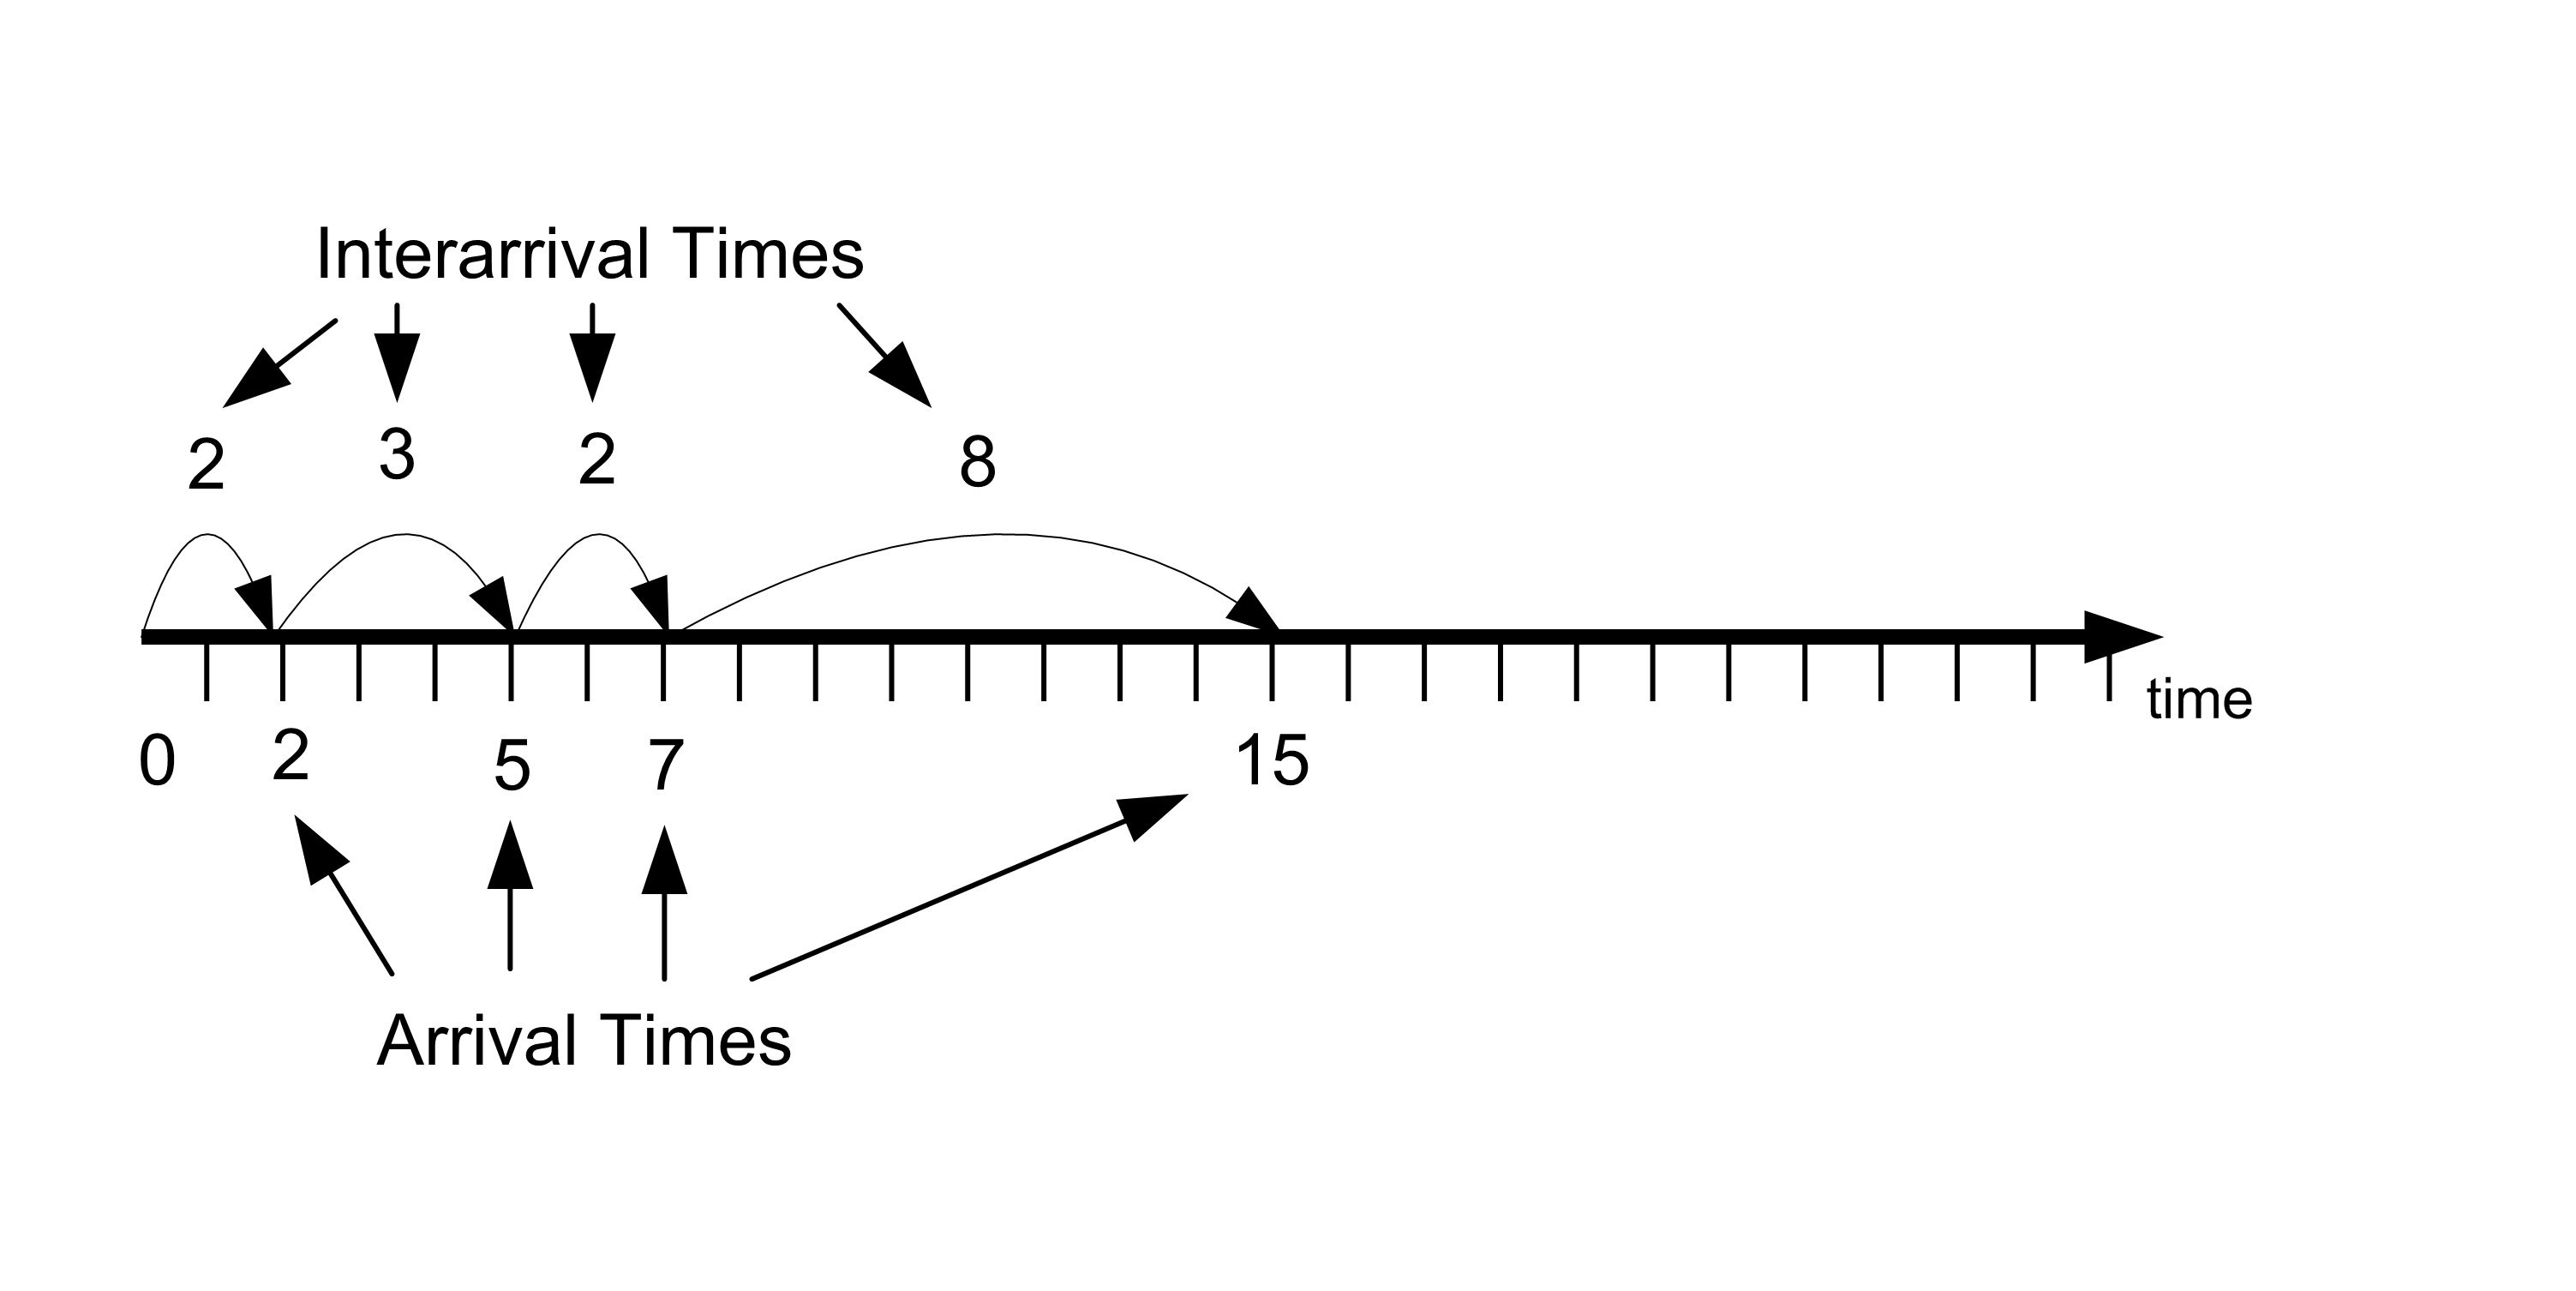
\includegraphics{./figures2/ch2/fig13ArrivalProcess} 

}

\caption{Customer Arrival Process}\label{fig:ArrivalProcess}
\end{figure}

\hypertarget{tab:CustArrivals}{}
\begin{longtable}[]{@{}ccc@{}}
\caption{\label{tab:CustArrivals} Customer Time of Arrivals}\tabularnewline
\toprule
Customer & Time of arrival & Time between arrival \\
\midrule
\endfirsthead
\toprule
Customer & Time of arrival & Time between arrival \\
\midrule
\endhead
1 & 2 & 2 \\
2 & 5 & 3 \\
3 & 7 & 2 \\
4 & 15 & 8 \\
\bottomrule
\end{longtable}

Figure~\ref{fig:ArrivalProcess} illustrates a time line of customer
arrival events. The values for the arrival times in Table \ref{tab:CustArrivals} have been rounded to
whole numbers, but in general the arrival times can be any real valued
numbers greater than zero. According to the figure, the first customer
arrives at time two and there is an elapse of three minutes before
customer 2 arrives at time five. From the discrete-event perspective,
\emph{nothing} is happening in the bank from time \([0,2)\); however, at time 2, an
arrival event occurs and the subsequent actions associated with this
event need to be accounted for with respect to the state of the system. An event denotes an instance of time that changes the state of the system. Since an event causes actions that result in a change of system state,
it is natural to ask: What are the actions that occur when a customer arrives to the
bank?

\begin{itemize}
\item
  The customer enters the waiting line.
\item
  If there is an available teller, the customer will immediately exit
  the line and the available teller will begin to provide service.
\item
  If there are no tellers available, the customer will remain waiting
  in the line until a teller becomes available.
\end{itemize}

Now, consider the arrival of the first customer. Since the bank opens at
9 am with no customer and all the tellers idle, the first customer will
enter and immediately exit the queue at time 9:02 am (or time 2) and
then begin service. After the customer completes service, the customer
will exit the bank. When a customer completes service (and departs the
bank) the number of customers in the bank will decrease by one. It
should be clear that some actions need to occur when a customer
completes service. These actions correspond to the second event
associated with this system: the customer service completion event. What
are the actions that occur at this event?

\begin{itemize}
\item
  The customer departs the bank.
\item
  If there are waiting customers, the teller indicates to the next
  customer that he/she will serve the customer. The customer will exit
  the waiting line and will begin service with the teller.
\item
  If there are no waiting customers, then the teller will become idle.
\end{itemize}

Figure~\ref{fig:ServiceProcess} contains the service times for each
of the four customers that arrived in
Figure~\ref{fig:ArrivalProcess}. Examine the figure with respect to
customer 1. Based on the figure, customer 1 can enter service at time
two because there were no other customers present in the bank. Suppose
that it is now 9:02 am (time 2) and that the service time of customer 1
is known \emph{in advance} to be 8 minutes as indicated in Table \ref{tab:CustServiceTimes}. From this information, the time that customer 1 is going to complete service can be pre-computed. From
the information in the figure, customer 1 will complete service at time
10 (current time + service time = 2 + 8 = 10). Thus, it should be
apparent, that for you to recreate the bank's behavior over a time
period that you must have knowledge of the customer's service times. The
service time of each customer coupled with the knowledge of when the
customer began service allows the time that the customer will complete
service and depart the bank to be computed in advance. A careful
inspection of Figure~\ref{fig:ServiceProcess} and knowledge of how banks operate
should indicate that a customer will begin service either immediately
upon arrival (when a teller is available) or coinciding with when
another customer departs the bank after being served. This latter
situation occurs when the queue is not empty after a customer completes
service. The times that service completions occur and the times that
arrivals occur constitute the pertinent events for simulating this
banking system.

\begin{figure}

{\centering 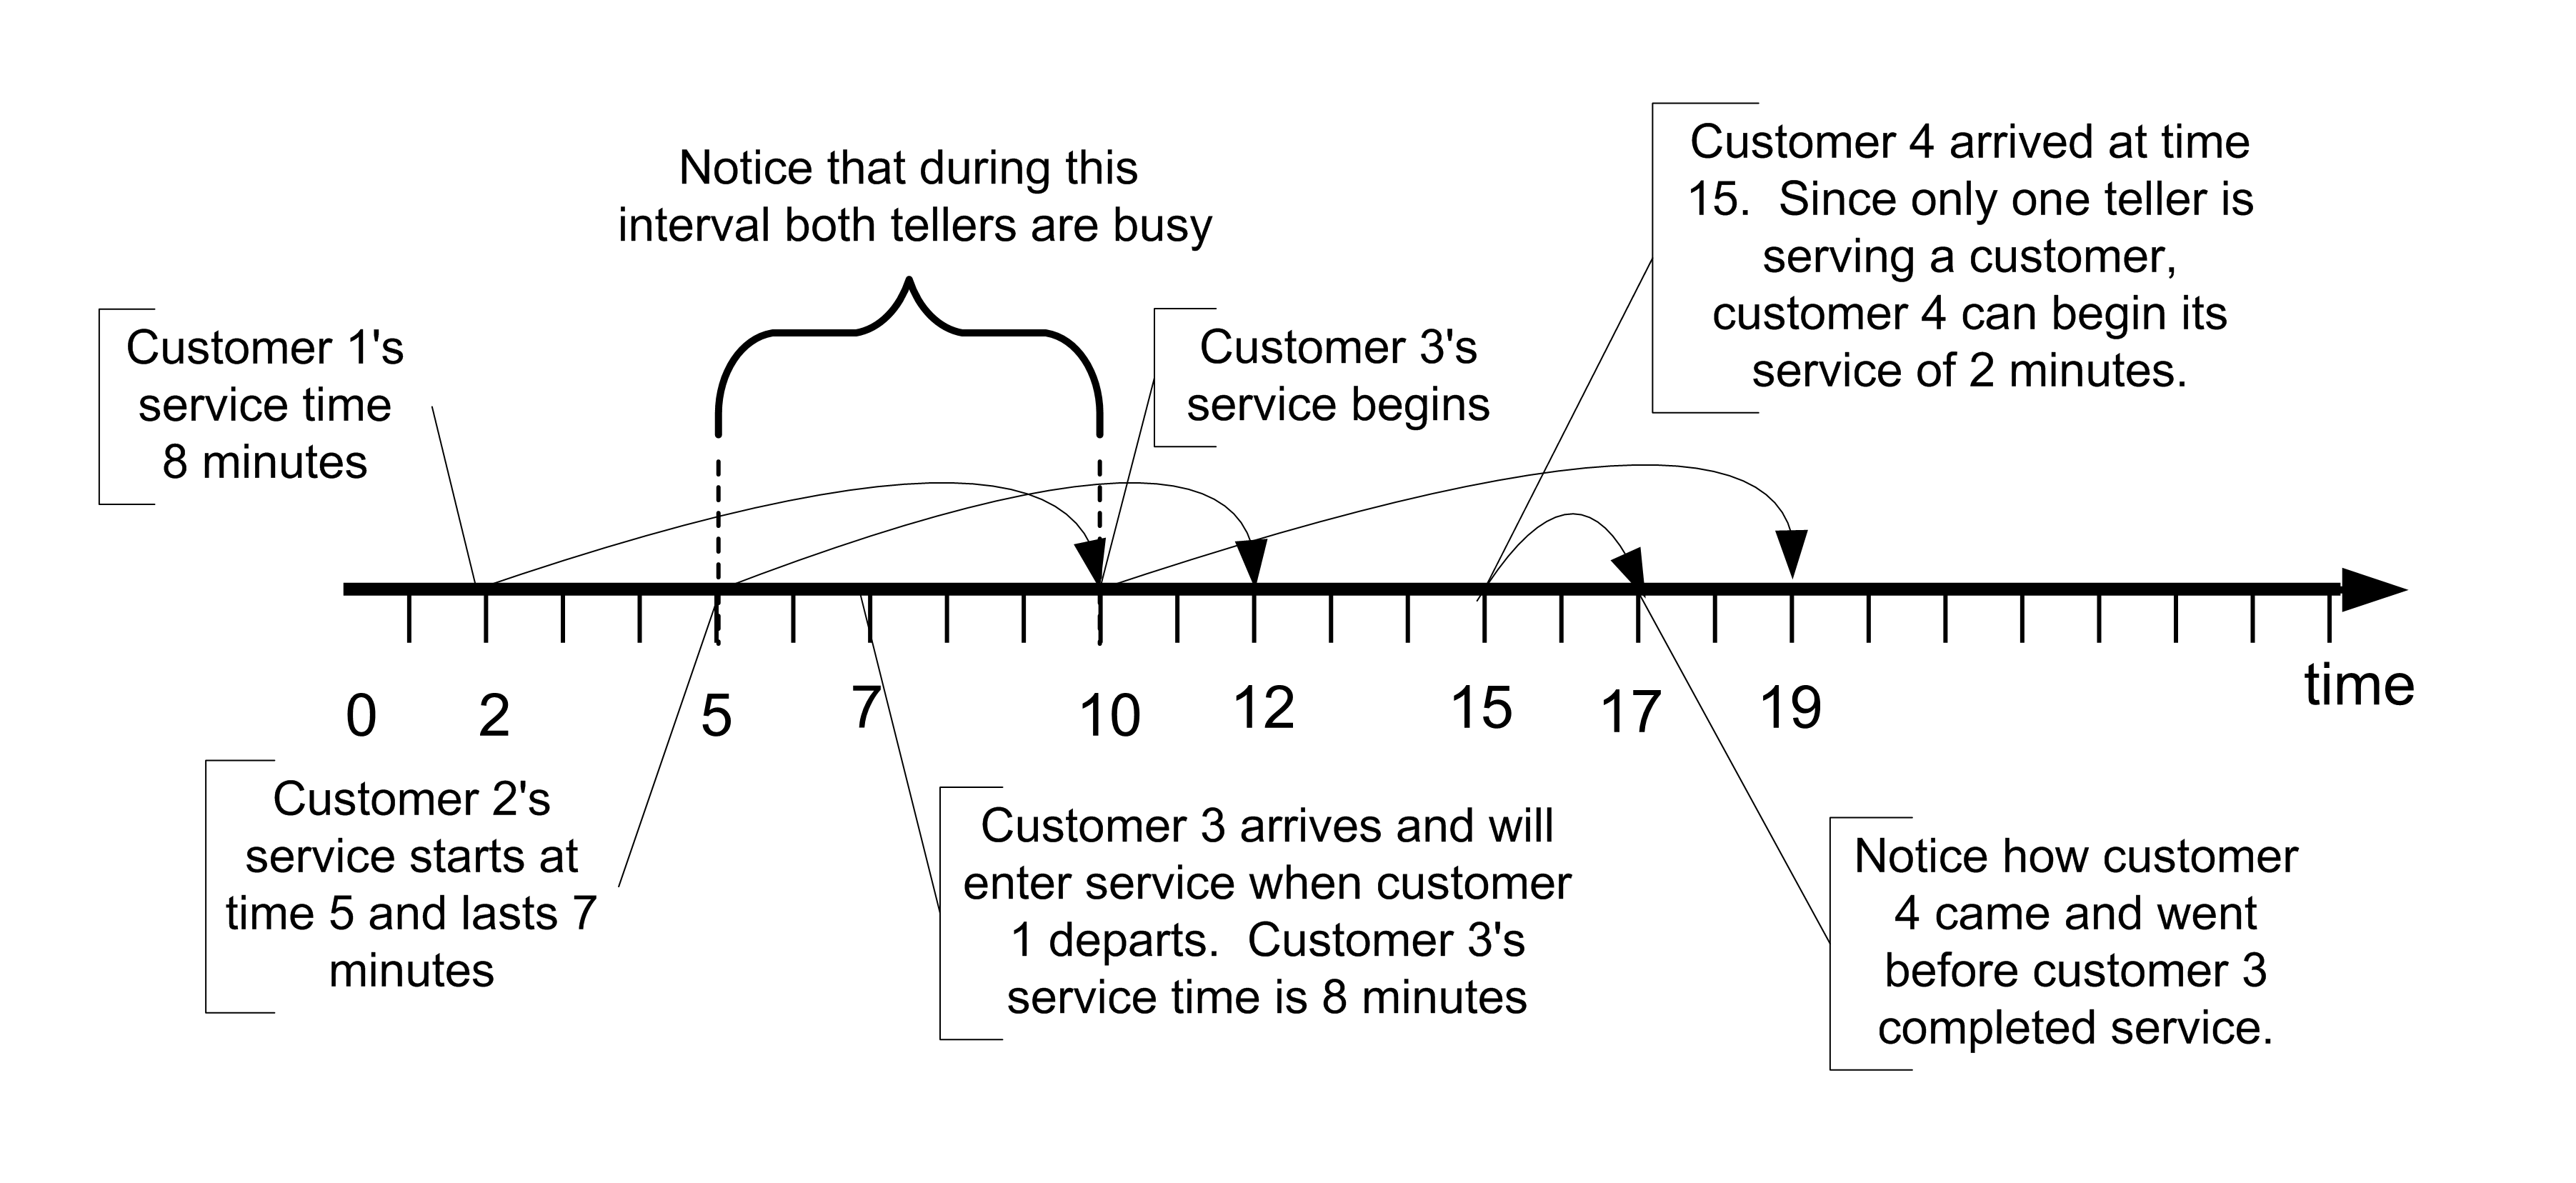
\includegraphics{./figures2/ch2/fig14ServiceProcess} 

}

\caption{Customer Service Process}\label{fig:ServiceProcess}
\end{figure}

\hypertarget{tab:CustServiceTimes}{}
\begin{longtable}[]{@{}cccc@{}}
\caption{\label{tab:CustServiceTimes} Service Time for First Four Customers}\tabularnewline
\toprule
Customer & Service Time Started & Service Time & Service Time Completed \\
\midrule
\endfirsthead
\toprule
Customer & Service Time Started & Service Time & Service Time Completed \\
\midrule
\endhead
1 & 2 & 8 & 10 \\
2 & 5 & 7 & 12 \\
3 & 10 & 9 & 19 \\
4 & 15 & 2 & 17 \\
\bottomrule
\end{longtable}

If the arrival and the service completion events are combined, then the
time ordered sequence of events for the system can be determined.
Figure~\ref{fig:TimeOrderedProcess} illustrates the events ordered by time
from smallest event time to largest event time. Suppose you are standing
at time two. Looking forward, the next event to occur will be at time 5
when the second customer arrives. When you simulate a system, you must
be able to generate a sequence of events so that, at the occurrence of
each event, the appropriate actions are invoked that change the state of
the system.

\begin{figure}

{\centering 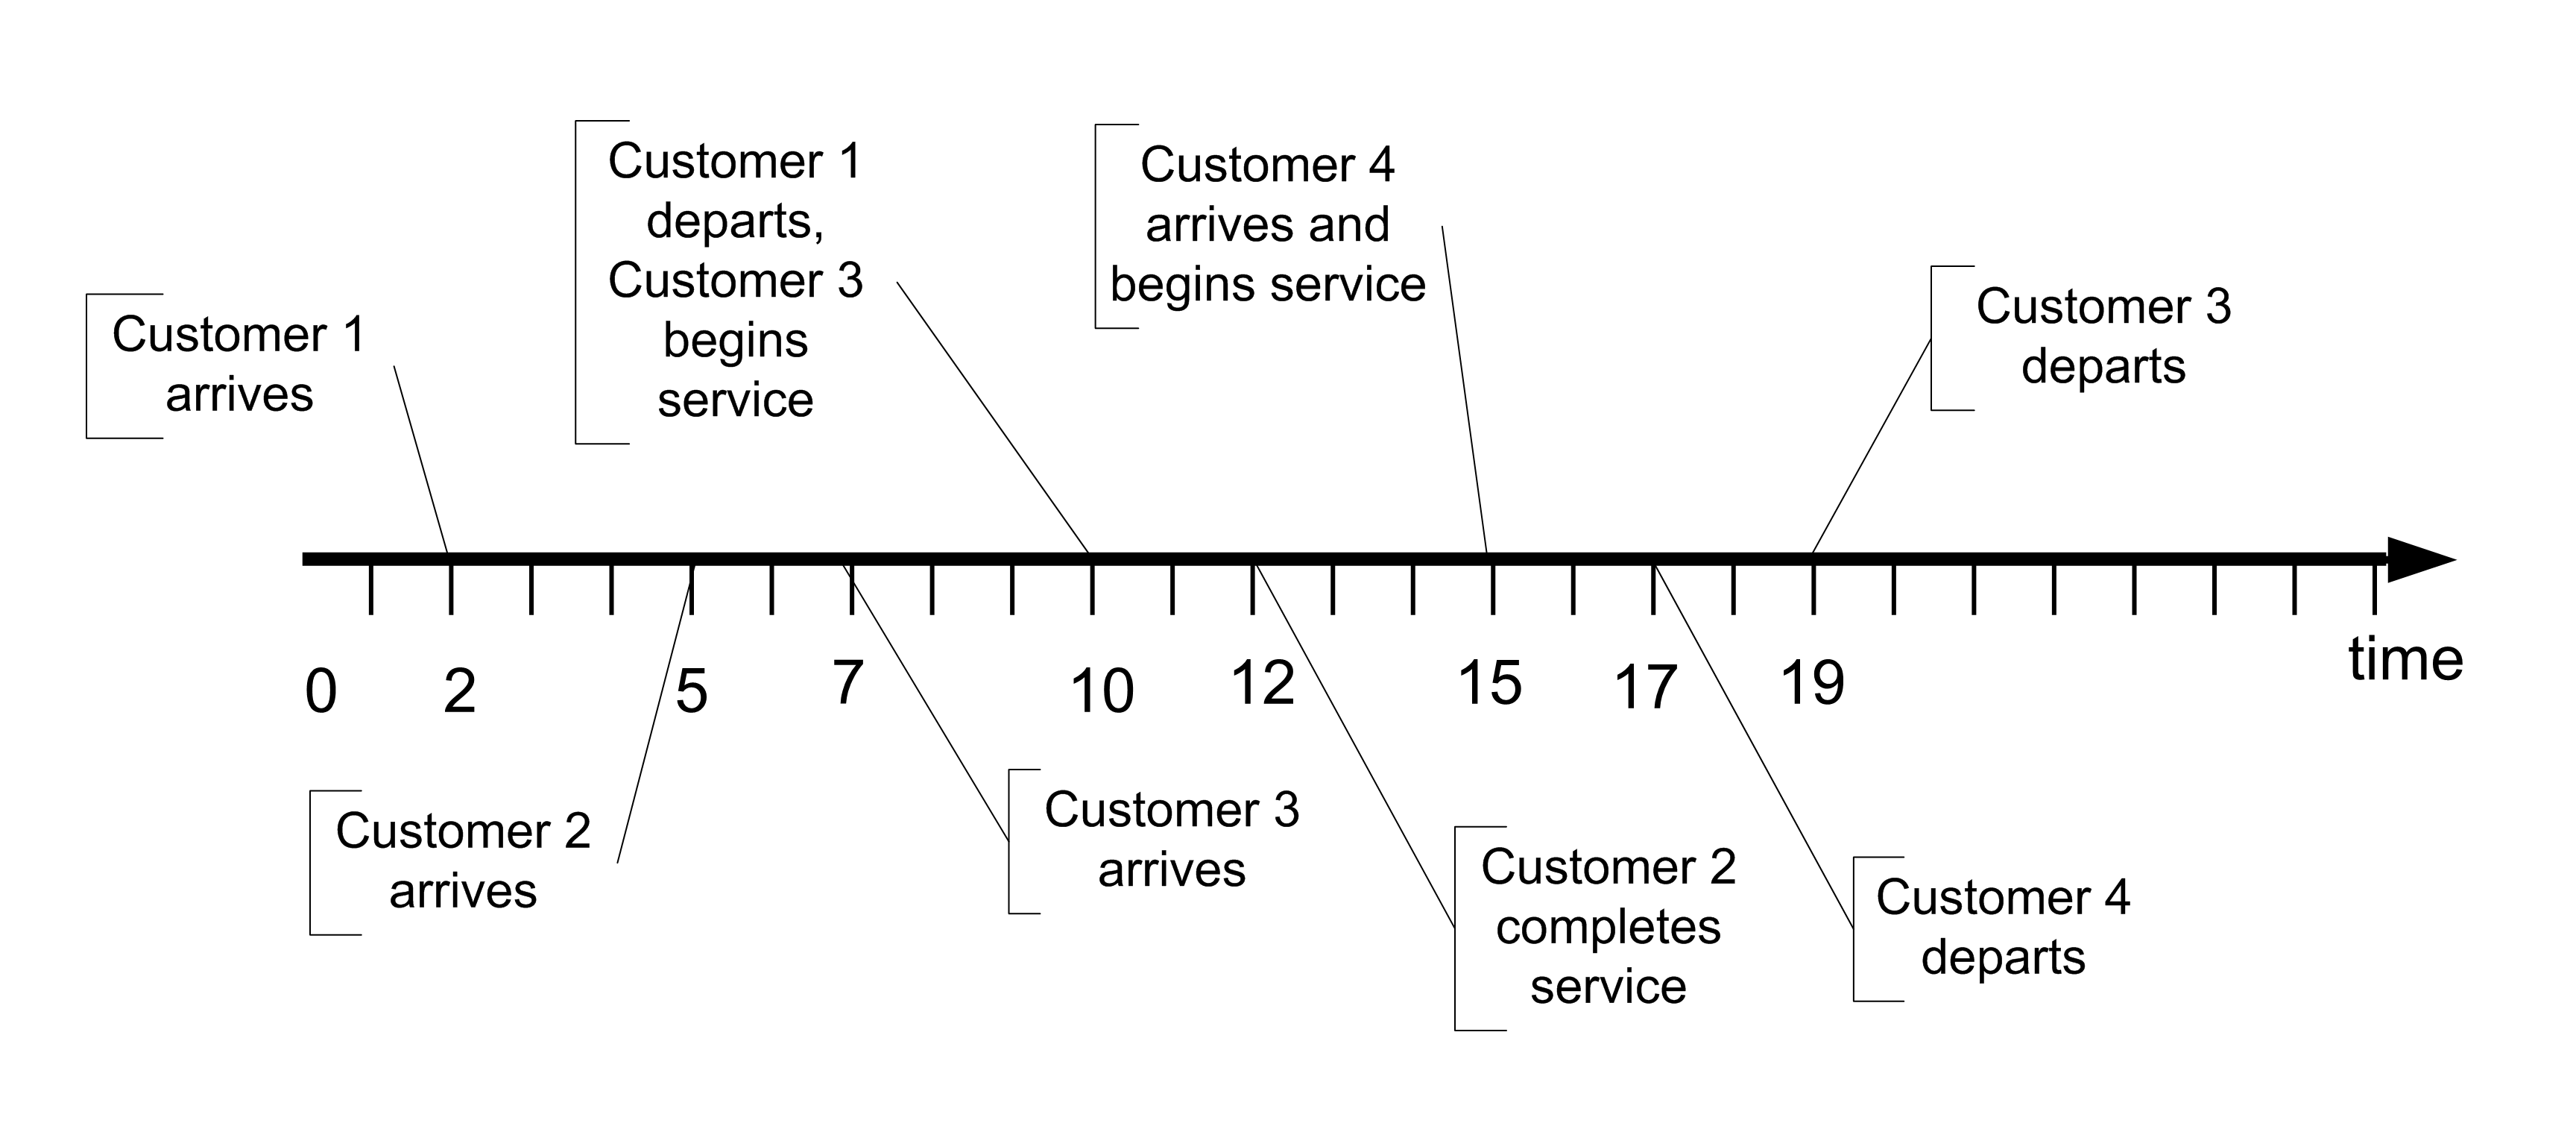
\includegraphics{./figures2/ch2/fig15TimeOrderedProcess} 

}

\caption{Events Ordered by Time Process}\label{fig:TimeOrderedProcess}
\end{figure}

\begin{longtable}[]{@{}ccl@{}}
\toprule
Time & Event & Comment \\
\midrule
\endhead
0 & Bank 0pens & \\
2 & Arrival & Customer 1 arrives, enters service for 8 minutes, one teller becomes busy \\
5 & Arrival & Customer 2 arrives, enters service for 7 minutes, the second teller becomes busy \\
7 & Arrival & Customer 3 arrives, waits in queue \\
10 & Service Completion & Customer 1 completes service, customer 3 exits the queue and enters service for 9 minutes \\
12 & Service Completion & Customer 2 completes service, no customers are in the queue so a teller becomes idle \\
15 & Arrival & Customer 4 arrives, enters service for 2 minutes, one teller becomes busy \\
17 & Service Completion & Customer 4 completes service, a teller becomes idle \\
19 & Service Completion & Customer 3 completes service \\
\bottomrule
\end{longtable}

\hfill\break

The real system will simply evolve over time; however, a simulation of
the system must recreate the events. In simulation, events are created
by adding additional logic to the normal state changing actions. This
additional logic is responsible for scheduling future events that are
implied by the actions of the current event. For example, when a
customer arrives, the time to the next arrival can be generated and
scheduled to occur at some future time. This can be done by generating
the time until the next arrival and adding it to the current time to
determine the actual arrival time. Thus, all the arrival times do not
need to be pre-computed prior to the start of the simulation. For
example, at time two, customer 1 arrived. Customer 2 arrives at time 5.
Thus, the time between arrivals (3 minutes) is added to the current time
and customer 2's arrival at time 5 is scheduled to occur. Every time an
arrival occurs this additional logic is invoked to ensure that more
arrivals will continue within the simulation.

Adding additional scheduling logic also occurs for service completion
events. For example, since customer 1 immediately enters service at time
2, the service completion of customer 1 can be scheduled to occur at
time 12 (current time + service time = 2 + 10 = 12). Notice that other
events may have already been scheduled for times less than time 12. In
addition, other events may be inserted before the service completion at
time 12 actually occurs. From this, you should begin to get a feeling
for how a computer program can implement some of these ideas.

Based on this intuitive notion for how a computer simulation may
execute, you should realize that computer logic processing need only
occur at the event times. That is, the state of the system does not
change between events. Thus, it is \emph{not necessary} to step incrementally
through time checking to see if something happens at time 0.1, 0.2, 0.3,
etc. (or whatever time scale you envision that is fine enough to not
miss any events). Thus, in a discrete-event dynamic system simulation the clock does not
``tick'' at regular intervals. Instead, the simulation clock jumps from
event time to event time. As the simulation moves from the current event
to the next event, the current simulation time is updated to the time of
the next event and any changes to the system associated with the next
event are executed. This allows the simulation to evolve over time.

\hypertarget{simulating-a-queueing-system-by-hand}{%
\section{Simulating a Queueing System By Hand}\label{simulating-a-queueing-system-by-hand}}

This section builds on the concepts discussed in the previous section in order to provide insights into how discrete event simulations operate. In order to do this, we will simulate a simple queueing system by hand. That is, we will process each of the events that occur as well as the state changes in order to trace the operation of the system through time.

Consider again the simple banking system described in the previous
section. To simplify the situation, we assume that there is only one
teller that is available to provide service to the arriving customers.
Customers that arrive while the teller is already helping a customer
form a single waiting line, which is handled in a first come, first
served manner. Let's assume that the bank opens at 9 am with no
customers present and the teller idle. The time of arrival of the first
eight customers is provided in the following table.

\begin{longtable}[]{@{}lll@{}}
\toprule
\endhead
Customer Number & Time of Arrival & Service Time \\
1 & 3 & 4 \\
2 & 11 & 4 \\
3 & 13 & 4 \\
4 & 14 & 3 \\
5 & 17 & 2 \\
6 & 19 & 4 \\
7 & 21 & 3 \\
8 & 27 & 2 \\
\bottomrule
\end{longtable}

We are going to process these customers in order to recreate the
behavior of this system over from time 0 to 31 minutes. To do this, we
need to be able to perform the ``bookkeeping'' that a computer simulation
model would normally perform for us. Thus, we will need to define some
variables associated with the system and some attributes associated with
the customers. Consider the following system variables.

System Variables

\begin{itemize}
\item
  Let \(t\) represent the current simulation clock time.
\item
  Let \(N(t)\) represent the number of customers in the system (bank) at
  any time \(t\).
\item
  Let \(Q(t)\) represent the number of customers waiting in line for the
  teller at any time \(t\).
\item
  Let \(B(t)\) represent whether or not the teller is busy (1) or
  idle (0) at any time \(t\).
\end{itemize}

Because we know the number of tellers available, we know that the
following relationship holds between the variables:

\[N\left( t \right) = Q\left( t \right) + B(t)\]

Note also that, knowledge of the value of \(N(t)\) is sufficient to
determine the values of \(Q(t)\) and \(B(t)\) at any time \(t.\) For example,
if we know that there are 3 customers in the bank, then
\(N\left( t \right) = 3\), and since the teller must be serving 1 of those
customers, \(B\left( t \right) = 1\) and there must be 2 customers
waiting, \(Q\left( t \right) = 2\). In this situation, since
\(N\left( t \right)\), is sufficient to determine all the other system
variables, we can say that \(N\left( t \right)\) is the system's \emph{state
variable}. The state variable(s) are the minimal set of system
variables that are necessary to represent the system's behavior over
time. We will keep track of the values of all of the system variables
during our processing in order to collect statistics across time.

Attributes are properties of things that move through the system. In the parlance of simulation, we call the things that move through the system entity instances or entities. In this situation, the entities are the customers, and we can define a number of attributes for each customer. Here, customer is a type of entity or entity type. If we have other things that flow through the system, we identity the different types (or entity types). The attributes of the customer entity type are as follows. Notice that each attribute is subscripted by \(i\), which indicates the \(i^{th}\) customer instance.

Entity Attributes

\begin{itemize}
\item
  Let \(\mathrm{ID}_{i}\) be the identity number of the customer.
  \(\mathrm{ID}_{i}\) is a unique number assigned to each customer that
  identifies the customer from other customers in the system.
\item
  Let \(A_{i}\) be the arrival time of the \(i^{\mathrm{th}}\) customer.
\item
  Let \(S_{i}\) be the time the \(i^{\mathrm{th}}\) customer started
  service.
\item
  Let \(D_{i}\) be the departure time of the \(i^{\mathrm{th}}\) customer.
\item
  Let \(\mathrm{ST}_{i}\) be the service time of the \(i^{\mathrm{th}}\)
  customer.
\item
  Let \(T_{i}\) be the total time spent in the system of the
  \(i^{\mathrm{th}}\) customer.
\item
  Let \(W_{i}\) be the time spent waiting in the queue for the
  \(i^{\mathrm{th}}\) customer.
\end{itemize}

Clearly, there are also relationships between these attributes. We can
compute the total time in the system for each customer from their
arrival and departure times:

\[T_{i} = D_{i} - A_{i}\]

In addition, we can compute the time spent waiting in the queue for each
customer as:

\[W_{i} = T_{i} - \mathrm{ST}_{i} = S_{i} - A_{i}\]

As in the previous section, there are two types of events: arrivals and
departures. Let \(E(t)\) be (A) for an arrival event at time \(t\) and be
(D) for a departure event at time \(t\). As we process each event, we will
keep track of when the event occurs and the type of event. We will also
keep track of the state of the system after each event has been
processed. To make this easier, we will keep track of the system
variables and the entity attributes within a table as follows.

\begin{table}

\caption{\label{tab:SQBH1}Hand Bank Simulation Bookkeeping Table.}
\centering
\fontsize{10}{12}\selectfont
\begin{tabular}[t]{rlrrrrrrrrrrl}
\toprule
\multicolumn{5}{c}{System Variables} & \multicolumn{7}{c}{Entity Attributes} & \multicolumn{1}{c}{ } \\
\cmidrule(l{3pt}r{3pt}){1-5} \cmidrule(l{3pt}r{3pt}){6-12}
t & E(t) & N(t) & B(t) & Q(t) & ID(i) & A(i) & S(i) & ST(i) & D(i) & T(i) & W(i) & Pending E(t)\\
\midrule
0 & NA & 0 & 0 & 0 & NA & NA & NA & NA & NA & NA & NA & NA\\
\bottomrule
\end{tabular}
\end{table}

In the table, we see that the initial state of the system is empty and
idle. Since there are no customers in the bank, there are no tabulated
attribute values within the table. Reviewing the provided information,
we see that customer 1 arrives at \(t = 3\) and has a service time of 4
minutes. Thus,\(\ \text{ID}_{1} = 1\), \(A_{1} = 3\), and
\(\text{ST}_{1} = 4\). We can enter this information directly into our
bookkeeping table. In addition, because the bank was empty and idle when
the customer arrived, we can note that the time that customer 1 starts
service is the same as the time of their arrival and that they did not
spend any time waiting in the queue. Thus, \(S_{1} = 3\) and \(W_{1} = 0\).
The table has been updated as follows.

\begin{table}

\caption{\label{tab:SQBH2}Hand Bank Simulation Bookkeeping Table.}
\centering
\fontsize{10}{12}\selectfont
\begin{tabular}[t]{rlrrrrrrrrrrl}
\toprule
\multicolumn{5}{c}{System Variables} & \multicolumn{7}{c}{Entity Attributes} & \multicolumn{1}{c}{ } \\
\cmidrule(l{3pt}r{3pt}){1-5} \cmidrule(l{3pt}r{3pt}){6-12}
t & E(t) & N(t) & B(t) & Q(t) & ID(i) & A(i) & S(i) & ST(i) & D(i) & T(i) & W(i) & Pending E(t)\\
\midrule
0 & NA & 0 & 0 & 0 & NA & NA & NA & NA & NA & NA & NA & NA\\
3 & A & 1 & 1 & 0 & 1 & 3 & 4 & 3 & NA & NA & 0 & E(7) = D(1), E(11) = A(2)\\
\bottomrule
\end{tabular}
\end{table}

Because customer 1 arrived to an empty system, they immediately started
service at time 3. Since we know the service time of the customer,
\(\text{ST}_{1} = 4\), and the current time, \(t = 3\), we can determine
that customer 1, will depart from the system at time 7
(\(t = 3 + 4 = 7\)). That means we will have a departure event for
customer 1 at time 7. According to the provided data, the next customer,
customer 2, will arrive at time 11. Thus, we have two pending events, a
departure of customer 1 at time 7 and the arrival of customer 2 at time
11. This fact is noted in the column labeled ``Pending E(t)'' for pending events. Here
E(7) = D(1), E(11) = A(2) indicates that customer 1 with
depart,\(\ D_{1},\) at time 7, \(E\left( 7 \right)\) and customer 2 will
arrive, \(A_{2}\), at the event at time 11, \(E(11)\). Clearly, the next
event time will be the minimum of 7 and 11, which will be the departure
of the first customer. Thus, our bookkeeping table can be updated as
follows.

\begin{table}

\caption{\label{tab:SQBH3}Hand Bank Simulation Bookkeeping Table.}
\centering
\fontsize{10}{12}\selectfont
\begin{tabular}[t]{rlrrrrrrrrrrl}
\toprule
\multicolumn{5}{c}{System Variables} & \multicolumn{7}{c}{Entity Attributes} & \multicolumn{1}{c}{ } \\
\cmidrule(l{3pt}r{3pt}){1-5} \cmidrule(l{3pt}r{3pt}){6-12}
t & E(t) & N(t) & B(t) & Q(t) & ID(i) & A(i) & S(i) & ST(i) & D(i) & T(i) & W(i) & Pending E(t)\\
\midrule
0 & NA & 0 & 0 & 0 & NA & NA & NA & NA & NA & NA & NA & NA\\
3 & A & 1 & 1 & 0 & 1 & 3 & 4 & 3 & NA & NA & 0 & E(7) = D(1), E(11) = A(2)\\
7 & D & 0 & 0 & 0 & 1 & 3 & 4 & 3 & 7 & 4 & 0 & E(11) = A(2)\\
\bottomrule
\end{tabular}
\end{table}

Since there are no customers in the bank and only the one pending event,
the next event will be the arrival of customer 2 at time 11. The table
can be updated as follows.

\begin{table}

\caption{\label{tab:SQBH4}Hand Bank Simulation Bookkeeping Table.}
\centering
\fontsize{10}{12}\selectfont
\begin{tabular}[t]{rlrrrrrrrrrrl}
\toprule
\multicolumn{5}{c}{System Variables} & \multicolumn{7}{c}{Entity Attributes} & \multicolumn{1}{c}{ } \\
\cmidrule(l{3pt}r{3pt}){1-5} \cmidrule(l{3pt}r{3pt}){6-12}
t & E(t) & N(t) & B(t) & Q(t) & ID(i) & A(i) & S(i) & ST(i) & D(i) & T(i) & W(i) & Pending E(t)\\
\midrule
0 & NA & 0 & 0 & 0 & NA & NA & NA & NA & NA & NA & NA & NA\\
3 & A & 1 & 1 & 0 & 1 & 3 & 4 & 3 & NA & NA & 0 & E(7) = D(1), E(11) = A(2)\\
7 & D & 0 & 0 & 0 & 1 & 3 & 4 & 3 & 7 & 4 & 0 & E(11) = A(2)\\
11 & A & 1 & 1 & 0 & 2 & 11 & 4 & 11 & NA & NA & 0 & E(13) = A(3), E(15) = D(2)\\
\bottomrule
\end{tabular}
\end{table}

Since the pending event set is E(13) = A(3), E(15) = D(2) the next event
will be the arrival of the third customer at time 13 before the
departure of the second customer at time 15. We will now have a queue
form. Updating our bookkeeping table, yields:

\begin{table}

\caption{\label{tab:SQBH5}Hand Bank Simulation Bookkeeping Table.}
\centering
\fontsize{10}{12}\selectfont
\begin{tabular}[t]{rlrrrrrrrrrrl}
\toprule
\multicolumn{5}{c}{System Variables} & \multicolumn{7}{c}{Entity Attributes} & \multicolumn{1}{c}{ } \\
\cmidrule(l{3pt}r{3pt}){1-5} \cmidrule(l{3pt}r{3pt}){6-12}
t & E(t) & N(t) & B(t) & Q(t) & ID(i) & A(i) & S(i) & ST(i) & D(i) & T(i) & W(i) & Pending E(t)\\
\midrule
0 & NA & 0 & 0 & 0 & NA & NA & NA & NA & NA & NA & NA & NA\\
3 & A & 1 & 1 & 0 & 1 & 3 & 4 & 3 & NA & NA & 0 & E(7) = D(1), E(11) = A(2)\\
7 & D & 0 & 0 & 0 & 1 & 3 & 4 & 3 & 7 & 4 & 0 & E(11) = A(2)\\
11 & A & 1 & 1 & 0 & 2 & 11 & 4 & 11 & NA & NA & 0 & E(13) = A(3), E(15) = D(2)\\
13 & A & 2 & 1 & 1 & 3 & 13 & 4 & 15 & NA & NA & 2 & E(14) = A(4), E(15) = D(2)\\
\bottomrule
\end{tabular}
\end{table}

Notice that in the last table update, we did not update \(S_{i}\) and
\(W_{i}\) because customer 3 had to wait in queue and did not start
service. Customer 3 will start service, when customer 2 departs.
Reviewing the pending event set, we see that the next event will be the
arrival of customer 4 at time 14, which yields the following bookkeeping
table.

\begin{table}

\caption{\label{tab:SQBH6}Hand Bank Simulation Bookkeeping Table.}
\centering
\fontsize{10}{12}\selectfont
\begin{tabular}[t]{rlrrrrrrrrrrl}
\toprule
\multicolumn{5}{c}{System Variables} & \multicolumn{7}{c}{Entity Attributes} & \multicolumn{1}{c}{ } \\
\cmidrule(l{3pt}r{3pt}){1-5} \cmidrule(l{3pt}r{3pt}){6-12}
t & E(t) & N(t) & B(t) & Q(t) & ID(i) & A(i) & S(i) & ST(i) & D(i) & T(i) & W(i) & Pending E(t)\\
\midrule
0 & NA & 0 & 0 & 0 & NA & NA & NA & NA & NA & NA & NA & NA\\
3 & A & 1 & 1 & 0 & 1 & 3 & 4 & 3 & NA & NA & 0 & E(7) = D(1), E(11) = A(2)\\
7 & D & 0 & 0 & 0 & 1 & 3 & 4 & 3 & 7 & 4 & 0 & E(11) = A(2)\\
11 & A & 1 & 1 & 0 & 2 & 11 & 4 & 11 & NA & NA & 0 & E(13) = A(3), E(15) = D(2)\\
13 & A & 2 & 1 & 1 & 3 & 13 & 4 & 15 & NA & NA & 2 & E(14) = A(4), E(15) = D(2)\\
\addlinespace
14 & A & 3 & 1 & 2 & 4 & 14 & 3 & 19 & NA & NA & 5 & E(15) = D(2), E(17) = A(5)\\
\bottomrule
\end{tabular}
\end{table}

Notice that we now have 3 customers in the system, 1 in service and 2
waiting in the queue. Reviewing the pending event set, we see that
customer 2 will finally complete service and depart at time 15.

\begin{table}

\caption{\label{tab:SQBH7}Hand Bank Simulation Bookkeeping Table.}
\centering
\fontsize{10}{12}\selectfont
\begin{tabular}[t]{rlrrrrrrrrrrl}
\toprule
\multicolumn{5}{c}{System Variables} & \multicolumn{7}{c}{Entity Attributes} & \multicolumn{1}{c}{ } \\
\cmidrule(l{3pt}r{3pt}){1-5} \cmidrule(l{3pt}r{3pt}){6-12}
t & E(t) & N(t) & B(t) & Q(t) & ID(i) & A(i) & S(i) & ST(i) & D(i) & T(i) & W(i) & Pending E(t)\\
\midrule
0 & NA & 0 & 0 & 0 & NA & NA & NA & NA & NA & NA & NA & NA\\
3 & A & 1 & 1 & 0 & 1 & 3 & 4 & 3 & NA & NA & 0 & E(7) = D(1), E(11) = A(2)\\
7 & D & 0 & 0 & 0 & 1 & 3 & 4 & 3 & 7 & 4 & 0 & E(11) = A(2)\\
11 & A & 1 & 1 & 0 & 2 & 11 & 4 & 11 & NA & NA & 0 & E(13) = A(3), E(15) = D(2)\\
13 & A & 2 & 1 & 1 & 3 & 13 & 4 & 15 & NA & NA & 2 & E(14) = A(4), E(15) = D(2)\\
\addlinespace
14 & A & 3 & 1 & 2 & 4 & 14 & 3 & 19 & NA & NA & 5 & E(15) = D(2), E(17) = A(5)\\
15 & D & 2 & 1 & 1 & 2 & 11 & 4 & 11 & 15 & 4 & 0 & E(17) = A(5), E(19) = D(3)\\
\bottomrule
\end{tabular}
\end{table}

Because customer 2 completes service at time 15 and customer 3 is
waiting in the line, we see that customer 3's attributes for \(S_{i}\) and
\(W_{i}\) were updated within the table. Since customer 3 has started
service and we know their service time of 4 minutes, we know that they
will depart at time 19. The pending events set has been updated
accordingly and indicates that the next event will be the arrival of
customer 5 at time 17.

\begin{table}

\caption{\label{tab:SQBH8}Hand Bank Simulation Bookkeeping Table.}
\centering
\fontsize{10}{12}\selectfont
\begin{tabular}[t]{rlrrrrrrrrrrl}
\toprule
\multicolumn{5}{c}{System Variables} & \multicolumn{7}{c}{Entity Attributes} & \multicolumn{1}{c}{ } \\
\cmidrule(l{3pt}r{3pt}){1-5} \cmidrule(l{3pt}r{3pt}){6-12}
t & E(t) & N(t) & B(t) & Q(t) & ID(i) & A(i) & S(i) & ST(i) & D(i) & T(i) & W(i) & Pending E(t)\\
\midrule
0 & NA & 0 & 0 & 0 & NA & NA & NA & NA & NA & NA & NA & NA\\
3 & A & 1 & 1 & 0 & 1 & 3 & 4 & 3 & NA & NA & 0 & E(7) = D(1), E(11) = A(2)\\
7 & D & 0 & 0 & 0 & 1 & 3 & 4 & 3 & 7 & 4 & 0 & E(11) = A(2)\\
11 & A & 1 & 1 & 0 & 2 & 11 & 4 & 11 & NA & NA & 0 & E(13) = A(3), E(15) = D(2)\\
13 & A & 2 & 1 & 1 & 3 & 13 & 4 & 15 & NA & NA & 2 & E(14) = A(4), E(15) = D(2)\\
\addlinespace
14 & A & 3 & 1 & 2 & 4 & 14 & 3 & 19 & NA & NA & 5 & E(15) = D(2), E(17) = A(5)\\
15 & D & 2 & 1 & 1 & 2 & 11 & 4 & 11 & 15 & 4 & 0 & E(17) = A(5), E(19) = D(3)\\
17 & A & 3 & 1 & 2 & 5 & 17 & 2 & 22 & NA & NA & 5 & E(19) = D(3), E(19) = A(6)\\
\bottomrule
\end{tabular}
\end{table}

Now, we have a very interesting situation with the pending event set. We
have two events that are scheduled to occur at the same time, the
departure of customer 3 at time 19 and the arrival of customer 6 at time
19. In general, the order in which events are processed that occur at
the same time may affect how future events are processed. That is, the
order of event processing may change the behavior of the system over
time and thus the order of processing is, in general, important.
However, in this particular simple system, the order of processing will
not change what happens in the future. We will simply have an update of
the state variables at the same time. In this instance, we will process
the departure event first and then the arrival event. If you are not
convinced that this will not make a difference, then I encourage you to
change the ordering and continue the processing. In more complex system
simulations, a priority indicator is attached to the events so that the
events can be processed in a consistent manner. Rather than continuing
the step-by-step processing of the events through time 31, we will
present the completed table. We leave it as an exercise for the reader
to continue the processing of the customers. The completed bookkeeping table at
time 31 is as follows.

\begin{table}

\caption{\label{tab:SQBHFull}Hand Bank Simulation Bookkeeping Table.}
\centering
\fontsize{10}{12}\selectfont
\begin{tabular}[t]{rlrrrrrrrrrrl}
\toprule
\multicolumn{5}{c}{System Variables} & \multicolumn{7}{c}{Entity Attributes} & \multicolumn{1}{c}{ } \\
\cmidrule(l{3pt}r{3pt}){1-5} \cmidrule(l{3pt}r{3pt}){6-12}
t & E(t) & N(t) & B(t) & Q(t) & ID(i) & A(i) & S(i) & ST(i) & D(i) & T(i) & W(i) & Pending E(t)\\
\midrule
0 & NA & 0 & 0 & 0 & NA & NA & NA & NA & NA & NA & NA & NA\\
3 & A & 1 & 1 & 0 & 1 & 3 & 4 & 3 & NA & NA & 0 & E(7) = D(1), E(11) = A(2)\\
7 & D & 0 & 0 & 0 & 1 & 3 & 4 & 3 & 7 & 4 & 0 & E(11) = A(2)\\
11 & A & 1 & 1 & 0 & 2 & 11 & 4 & 11 & NA & NA & 0 & E(13) = A(3), E(15) = D(2)\\
13 & A & 2 & 1 & 1 & 3 & 13 & 4 & 15 & NA & NA & 2 & E(14) = A(4), E(15) = D(2)\\
\addlinespace
14 & A & 3 & 1 & 2 & 4 & 14 & 3 & 19 & NA & NA & 5 & E(15) = D(2), E(17) = A(5)\\
15 & D & 2 & 1 & 1 & 2 & 11 & 4 & 11 & 15 & 4 & 0 & E(17) = A(5), E(19) = D(3)\\
17 & A & 3 & 1 & 2 & 5 & 17 & 2 & 22 & NA & NA & 5 & E(19) = D(3), E(19) = A(6)\\
19 & D & 2 & 1 & 1 & 3 & 13 & 4 & 15 & 19 & 6 & 2 & E(19) = A(6)\\
19 & A & 3 & 1 & 2 & 6 & 19 & 4 & 24 & NA & NA & 5 & E(21) = A(7), E(22) = D(4)\\
\addlinespace
21 & A & 4 & 1 & 3 & 7 & 21 & 3 & 28 & NA & NA & 7 & E(22) = D(4), E(24) = D(5)\\
22 & D & 3 & 1 & 2 & 4 & 14 & 3 & 19 & 22 & 8 & 5 & E(24) = D(5), E(27) = A(8)\\
24 & D & 2 & 1 & 1 & 5 & 17 & 2 & 22 & 24 & 7 & 5 & E(27) = A(8), E(28) = D(6)\\
27 & A & 3 & 1 & 2 & 8 & 27 & 2 & 31 & NA & NA & 4 & E(28) = D(6), E(31) = D(7)\\
28 & D & 2 & 1 & 1 & 6 & 19 & 4 & 24 & 28 & 9 & 5 & E(31) = D(7)\\
\addlinespace
31 & D & 1 & 1 & 0 & 7 & 21 & 3 & 28 & 31 & 10 & 7 & E(33) = D(8)\\
\bottomrule
\end{tabular}
\end{table}

Given that we have simulated the bank over the time frame from 0 to 31
minutes, we can now compute performance statistics for the bank and
measure how well it is operating. Two statistics that we can easily
compute are the average time spent waiting in line and the average time
spent in the system.

Let \(n\) be the number of customers observed to depart during the
simulation. In this simulation, we had \(n = 7\) customers depart during
the time frame of 0 to 31 minutes. The time frame over which we analyze
the performance of the system is call the simulation time horizon. In
this case, the simulation time horizon is fixed and known in advance.
When we perform a computer simulation experiment, the time horizon is
often referred to as the \emph{simulation run length} (or simulation
\emph{replication length}). To estimate the average time spent waiting in
line and the average time spent in the system, we can simply compute the
sample averages ( \(\overline{T}\) and \(\bar{W})\) of the observed
quantities (\(T_{i}\) and \(W_{i}\))for each departed customer.

\[\overline{T} = \frac{1}{7}\sum_{i = 1}^{7}T_{i} = \frac{4 + 4 + 6 + 8 + 7 + 9 + 10}{7} = \frac{48}{7} \cong 6.8571\]

\[\overline{W} = \frac{1}{7}\sum_{i = 1}^{7}W_{i} = \frac{0 + 0 + 2 + 5 + 5 + 5 + 7}{7} = \frac{24}{7} \cong 3.4286\]

Besides the average time spent in the system and the average time spent
waiting, we might also want to compute the average number of customers
in the system, the average number of customers in the queue, and the
average number of busy tellers. You might be tempted to simply average
the values in the \(N(t)\), \(B(t)\), and \(Q(t)\) columns of the bookkeeping table.
Unfortunately, that will result in an incorrect estimate of these values
because a simple average will not take into account how long each of the
variables persisted with its values over time. In this situation, we are
really interested in computed a time average. This is because the
variables, \(N(t)\), \(B(t)\), and \(Q(t)\) are time-based variables. This type of
variable is always encountered in discrete event simulations.

To make the discussion concrete, let's focus on the number of customers
in the queue, \(Q(t)\). Notice the number of customers in the queue, \(Q(t)\)
takes on constant values during intervals of time corresponding to when
the queue has a certain number of customers.
\(Q(t) = \{ 0,1,2,3,\ldots\}\). The values of \(Q(t)\) form a step
function in this particular case. The following figure illustrates the
step function nature of this type of variable. A realization of the
values of variable is called a sample path.

\begin{figure}

{\centering 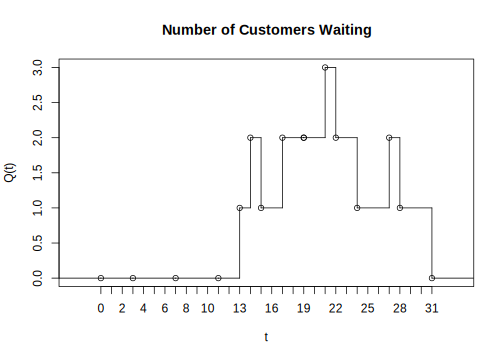
\includegraphics[width=0.7\linewidth]{06-introDEDS_files/figure-latex/NCInQ-1} 

}

\caption{Number of Customers Waiting in Queue for the Bank Simulation}\label{fig:NCInQ}
\end{figure}

That is, for a given (realized) sample path, \(Q(t)\) is a function that
returns the number of customers in the queue at time \(t\). The mean value
theorem of calculus for integrals states that given a function,
\(f( \bullet )\), continuous on an interval \((a, b)\), there exists a
constant, c, such that

\[\int_{a}^{b}{f\left( x \right)\text{dx}} = f(c)(b - a)\]

\[f\left( c \right) = \frac{\int_{a}^{b}{f\left( x \right)\text{dx}}}{(b - a)}\]

The value, \(f(c)\), is called the mean value of the function. A similar
function can be defined for \(Q(t)\) This function is called the
time-average (and represents the \emph{mean value} of the \(Q(t)\)
function):

\[\overline{Q}\left( n \right) = \frac{\int_{t_{0}}^{t_{n}}{Q\left( t \right)\text{dt}}}{t_{n} - t_{0}}\]

This function represents the \emph{average with respect to time} of the given
state variable. This type of statistical variable is called time-based
because \(Q(t)\) is a function of time.

In the particular case where \(Q(t)\) represents the number of customers
in the queue, \(Q(t)\) will take on constant values during intervals of
time corresponding to when the queue has a certain number of customers. Let \(Q\left( t \right) = \ q_{k}\ \)for\(\ t_{k - 1} \leq t \leq t_{k}\). Then, the time-average can be rewritten as follows:

\[\overline{Q}\left( t \right) = \frac{\int_{t_{0}}^{t_{n}}{Q\left( t \right)\text{dt}}}{t_{n} - t_{0}} = \sum_{k = 1}^{n}\frac{q_{k}(t_{k} - t_{k - 1})}{t_{n} - t_{0}}\]
Note that \(q_{k}(t_{k} - t_{k - 1})\) is the area under the curve, \(Q\left( t \right)\) over the interval \(t_{k - 1} \leq t \leq t_{k}\) and because \[t_{n} - t_{0} = \left( t_{1} - t_{0} \right) + \left( t_{2} - t_{1} \right) + \left( t_{3} - t_{2} \right) + \ \cdots + \left( t_{n - 1} - t_{n - 2} \right) + \ \left( t_{n} - t_{n - 1} \right)\]
we can write,
\[t_{n} - t_{0} = \sum_{k = 1}^{n}{t_{k} - t_{k - 1}}\]

The quantity \(t_{n} - t_{0}\) represents the total time over which the variable is observed. Thus, the time average is simply the area under the curve divided by the amount of time
over which the curve is observed. From this equation, it should be noted
that each value of \(q_{k}\) is weighted by the length of time that the
variable has the value. If we define, \(w_{k} = (t_{k} - t_{k - 1})\),
then we can re-write the time average as:

\[\overline{Q}\left( t \right) = \frac{\int_{t_{0}}^{t_{n}}{Q\left( t \right)\text{dt}}}{t_{n} - t_{0}} = \sum_{k = 1}^{n}\frac{q_{k}(t_{k} - t_{k - 1})}{t_{n} - t_{0}} = \frac{\sum_{k = 1}^{n}{q_{k}w_{k}}}{\sum_{i = 1}^{n}w_{k}}\]

This form of the equation clearly shows that each value of \(q_{k}\) is
weighted by:

\[\frac{w_{k}}{\sum_{i = 1}^{n}w_{k}} = \frac{w_{k}}{t_{n} - t_{0}} = \frac{(t_{k} - t_{k - 1})}{t_{n} - t_{0}}\]

This is why the time average is often called the time-weighted average.
If \(w_{k} = 1\), then the time-weighted average is the same as the sample
average.

Now we can compute the time average for
\(Q\left( t \right),\ N\left( t \right)\) and \(B(t)\). Using the following
formula and noting that \(t_{n} - t_{0} = 31\)

\[\overline{Q}\left( t \right) = \sum_{k = 1}^{n}\frac{q_{k}(t_{k} - t_{k - 1})}{t_{n} - t_{0}}\]

We have that the numerator computes as follows:

\[\sum_{k = 1}^{n}{q_{k}\left( t_{k} - t_{k - 1} \right)} = 0\left( 13 - 0 \right) + \ 1\left( 14 - 13 \right) + \ 2\left( 15 - 14 \right) + \ 1\left( 17 - 15 \right) + \ 2\left( 19 - 17 \right)\]

\[\  + 1\left( 19 - 19 \right) + \ 2\left( 21 - 19 \right) + \ 3\left( 22 - 21 \right) + \ 2\left( 24 - 22 \right) + \ \]

\[1\left( 27 - 24 \right) + \ 2\left( 28 - 27 \right) + \ 1\left( 31 - 28 \right) = 28\]

And, the final time-weighted average number in the queue ss:

\[\overline{Q}\left( t \right) = \frac{28}{31} \cong 0.903\]

The average number in the system and the average number of busy tellers
can also be computed in a similar manner, resulting in:

\[\overline{N}\left( t \right) = \frac{52}{31} \cong 1.677\]

\[\overline{B}\left( t \right) = \frac{24}{31} \cong 0.7742\]

The value of \(\overline{B}\left( t \right)\) is most interesting for this
situation. Because there is only 1 teller, the fraction of the tellers
that are busy is 0.7742. This quantity represents the \emph{utilization} of
the teller. The utilization of a resource represents the proportion of
time that the resource is busy. Let c represent the number of units of a
resource that are available. Then the utilization of the
resource is defined as:

\[\overline{U} = \frac{\overline{B}\left( t \right)}{c} = \frac{\int_{t_{0}}^{t_{n}}{B\left( t \right)\text{dt}}}{c(t_{n} - t_{0})}\]

Notice that the numerator of this equation is simply the total time that
the resource is busy. So, we are computing the total time that the
resource is busy divided by the total time that the resource could be
busy, \(c(t_{n} - t_{0})\), which is considered the utilization.

In this simple example, when an arrival occurs, you must determine
whether or not the customer will enter service or wait in the queue.
When a customer departs the system, whether or not the server will
become idle must be determined, by checking the queue. If the queue is
empty, then the server becomes idle; otherwise the next customer in the
queue begins service. In order to develop a computer simulation model of
this situation, the actions that occur at an event must be represented
within code. For example, the pseudo-code for the arrival event would
be:

\emph{Pseudo-code for Arrival Event}

\begin{enumerate}
\def\labelenumi{\arabic{enumi}.}
\item
  schedule arrival time of next customer

  \begin{enumerate}
  \def\labelenumii{\arabic{enumii}.}
  \item
    AT = generate time to next arrival according to inter-arrival
    distribution
  \item
    schedule arrival event at, t + AT
  \end{enumerate}
\item
  check status of the servers (idle or busy)

  \begin{enumerate}
  \def\labelenumii{\arabic{enumii}.}
  \item
    if idle, do

    \begin{enumerate}
    \def\labelenumiii{\arabic{enumiii}.}
    \item
      allocate a server to the customer
    \item
      ST = generate service time according to the service time
      distribution
    \item
      schedule departure event at, t + ST
    \end{enumerate}
  \item
    if busy, do

    \begin{enumerate}
    \def\labelenumiii{\arabic{enumiii}.}
    \tightlist
    \item
      increase number in queue by 1 (place customer in queue)
    \end{enumerate}
  \end{enumerate}
\end{enumerate}

\emph{Pseudo-code for Departure Event}

\begin{enumerate}
\def\labelenumi{\arabic{enumi}.}
\item
  if queue is not empty

  \begin{enumerate}
  \def\labelenumii{\arabic{enumii}.}
  \item
    remove next customer from the queue
  \item
    allocate the server to the next customer in the queue
  \item
    ST = generate service time according to the service time
    distribution
  \item
    schedule departure event at, t + ST
  \end{enumerate}
\item
  else the queue is empty

  \begin{enumerate}
  \def\labelenumii{\arabic{enumii}.}
  \tightlist
  \item
    make the customer's server idle
  \end{enumerate}
\end{enumerate}

Notice how the arrival event schedules the next arrival and the
departure event may schedule the next departure event (provided the
queue is not empty). Within the JSL, this pseudo-code must be
represented in a class method that will be called at the appropriate
event time.

To summarize, discrete-event modeling requires two key abilities:

\begin{itemize}
\item
  The ability to represent the actions associated with an event in
  computer code (i.e.~in a class method).
\item
  The ability to schedule events so that they will be called at the
  appropriate event time, i.e.~the ability to have the event's logic
  called at the appropriate event time.
\end{itemize}

Thus, the scheduling and execution of events is critical to
discrete-event modeling. The scheduling of additional events within an
event is what makes the system progress through time (jumping from event
to event). The JSL supports the scheduling and execution of events
within its calendar and model packages. The next section overviews the
libraries available within the JSL for discrete-event modeling.

\hypertarget{introDEDS:dedsJSL}{%
\section{Modeling DEDS in the JSL}\label{introDEDS:dedsJSL}}

Discrete event modeling within the JSL is facilitated by two packages:
1) the \texttt{jsl.simulation} package and 2) the \texttt{jsl.calendar} package. The \texttt{jsl.simulation}
package has classes that implement behavior associated with simulation
events and models. The \texttt{jsl.calendar} package has classes that facilitate the
scheduling and processing of events.

\hypertarget{event-scheduling}{%
\subsection{Event Scheduling}\label{event-scheduling}}

The following classes within the \texttt{jsl.simulation} package work together to
provide for the scheduling and execution of events:

\begin{itemize}
\item
  \texttt{Simulation} - An instance of Simulation holds the model and
  facilitates the running of the simulation according to run
  parameters such as simulation run length and number of replications.
\item
  \texttt{Executive} - The Executive controls the execution of the events and
  works with the calendar package to ensure that events are executed
  and the appropriate model logic is called at the appropriate event
  time. This class is responsible for placing the events on a
  calendar, allowing events to be canceled, and executing the events
  in the correct order.
\item
  \texttt{JSLEvent} -- This class represents a simulation event. The
  attributes of JSLEvent provide information about the name, time,
  priority, and type of the event. The user can also check whether or
  not the event is canceled or if it has been scheduled. In addition,
  a general attribute of type Object is associated with an event and
  can be used to pass information along with the event.
\item
  \texttt{ModelElement} -- This class serves as a base class for all classes
  that are within a simulation model. It provides access to the
  scheduler and ensures that model elements participate in common
  simulation actions (e.g.~warm up, initialization, etc.).
\item
  \texttt{Model} - An instance of a Model is required to serve as the parent
  to any model elements within a simulation model. It is the top-level
  container for model elements.
\item
  \texttt{SchedulingElement} -- SchedulingElement is a sub-class of
  ModelElement and facilitates the scheduling of events within a
  simulation model. Classes that require significant event scheduling
  should sub-class from SchedulingElement.
\end{itemize}

Figure \ref{fig:jslModeling} illustrates the relationships between the
classes \texttt{Model}, \texttt{ModelElement}, \texttt{SchedulingElement}, \texttt{Simulation}, and
\texttt{Executive.} The \texttt{ModelElement} class represents the primary building block
for JSL models. A \texttt{ModelElement} represents something (an element) that
can be placed within an instance of a \texttt{Model}. The \texttt{Model} class subclasses
\texttt{ModelElement}. Every \texttt{ModelElement} can contain many other instances of
\texttt{ModelElement}. As such, an instance of a \texttt{Model} can also contain model
elements. There can only be one instance of the \texttt{Model} class within the
simulation. It acts as the parent (container) for all other model
elements. Model elements in turn also hold other model elements.
Instances arranged in this pattern form an object hierarchy that
represents the simulation model. The instance of a Simulation holds
(references) the instance of the \texttt{Model} class. \texttt{Simulation} also references
the \texttt{Executive.} The instance of the \texttt{Executive} uses an instance of a class
that implements the \texttt{CalendarIfc} interface. The simulation also
references an instance of the \texttt{Experiment} class. The \texttt{Experiment} class
allows the specification and control of the run parameters for the
simulation. Every instance of a \texttt{ModelElement} must be a child of another
\texttt{ModelElement} or the \texttt{Model}. This implies that instances of \texttt{ModelElement}
have access to the main model, which has access to an instance of
\texttt{Simulation} and thus the instance of the \texttt{Executive}. Therefore sub-classes
of \texttt{ModelElement} have access to the \texttt{Executive} and can schedule events.

\begin{figure}
\centering
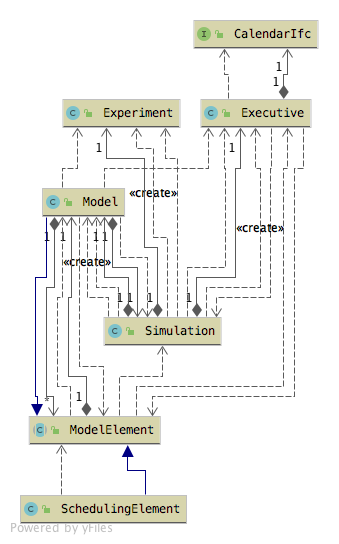
\includegraphics{./figures/ch4/jslmodeling.png}
\caption{\label{fig:jslModeling}jsl.simulation Package and Relationships}
\end{figure}

The \texttt{SchedulingElement} class is a special kind of \texttt{ModelElement} that
facilitates the scheduling of events. \texttt{SchedulingElement} is an abstract
base class for building other classes that schedule events. Sub-classes
of the \texttt{SchedulingElement} class will have a set of methods that
facilitate the scheduling of events.

\begin{figure}
\centering
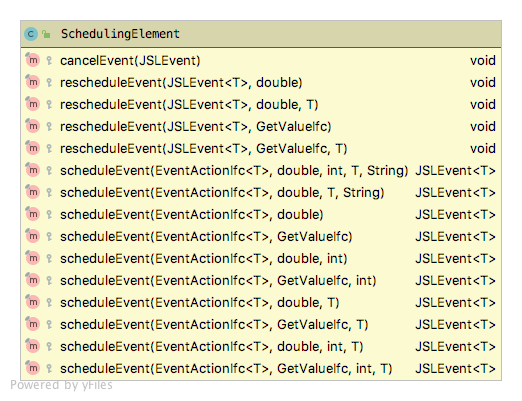
\includegraphics{./figures/ch4/SchedulingElement.png}
\caption{\label{fig:SchedulingElement}SchedulingElement and its scheduling methods}
\end{figure}

Figure \ref{fig:SchedulingElement} illustrates the protected methods of
the \texttt{SchedulingElement} class. Since these methods are protected,
sub-classes will have them available through inheritance. There are two
major types of scheduling methods: one for rescheduling already existing
events and another for scheduling new events. The scheduling of new
events results in the creation of a new \texttt{JSLEvent} and the placement of
the event on the event calendar via the \texttt{Executive.}

The following code listing illustrates the key method for
scheduling events within the class SchedulingElement. Notice that the instance of the \texttt{Executive} is called via \texttt{getExecutive()}. In addition, the user can supply information for the
creation of an event such as its time, name, and priority. The user can
also provide an instance of classes that implement the \texttt{EventActionIfc}
interface. This interface promises to have an \texttt{action()} method. Within
the \texttt{action()} method the user can provide the code that is necessary to
represent the state changes associated with the event.

\begin{Shaded}
\begin{Highlighting}[]
\CommentTok{/**}\NormalTok{ Creates an event and schedules it onto the event calendar}\CommentTok{. }\NormalTok{ This is the main scheduling method that}
 \CommentTok{*}\NormalTok{ all other scheduling methods call}\CommentTok{.}\NormalTok{  The other methods are just convenience methods for this method}\CommentTok{.}
 \CommentTok{*}
 \CommentTok{*} \CommentTok{@}\NormalTok{param }\KeywordTok{\textless{}T\textgreater{}}\NormalTok{ the type associated with the attached message}
 \CommentTok{*} \CommentTok{@}\NormalTok{param action represents an ActionListener that will handle the change of state logic}
 \CommentTok{*} \CommentTok{@}\NormalTok{param time represents the inter}\CommentTok{{-}}\NormalTok{event time}\CommentTok{,}\NormalTok{ i}\CommentTok{.}\NormalTok{e}\CommentTok{.}\NormalTok{ the interval from the current time to when the}
 \CommentTok{*}\NormalTok{        event will need to occur}
 \CommentTok{*} \CommentTok{@}\NormalTok{param priority is used to influence the ordering of events}
 \CommentTok{*} \CommentTok{@}\NormalTok{param message is a generic Object that may represent data to be transmitted with the event}
 \CommentTok{*} \CommentTok{@}\NormalTok{param name the name of the event}
 \CommentTok{*} \CommentTok{@}\NormalTok{return a valid JSLEvent}
 \CommentTok{*/}
\KeywordTok{protected} \DataTypeTok{final} \OperatorTok{\textless{}}\NormalTok{T}\OperatorTok{\textgreater{}}\NormalTok{ JSLEvent}\OperatorTok{\textless{}}\NormalTok{T}\OperatorTok{\textgreater{}} \FunctionTok{scheduleEvent}\OperatorTok{(}\NormalTok{EventActionIfc}\OperatorTok{\textless{}}\NormalTok{T}\OperatorTok{\textgreater{}}\NormalTok{ action}\OperatorTok{,} \DataTypeTok{double}\NormalTok{ time}\OperatorTok{,} \DataTypeTok{int}\NormalTok{ priority}\OperatorTok{,}\NormalTok{ T message}\OperatorTok{,} \BuiltInTok{String}\NormalTok{ name}\OperatorTok{)} \OperatorTok{\{}
\NormalTok{    JSLEvent}\OperatorTok{\textless{}}\NormalTok{T}\OperatorTok{\textgreater{}}\NormalTok{ event }\OperatorTok{=} \FunctionTok{getExecutive}\OperatorTok{().}\FunctionTok{scheduleEvent}\OperatorTok{(}\NormalTok{action}\OperatorTok{,}\NormalTok{ time}\OperatorTok{,}\NormalTok{ priority}\OperatorTok{,}\NormalTok{ message}\OperatorTok{,}\NormalTok{ name}\OperatorTok{,} \KeywordTok{this}\OperatorTok{);}
    \ControlFlowTok{return} \OperatorTok{(}\NormalTok{event}\OperatorTok{);}
\OperatorTok{\}}
\end{Highlighting}
\end{Shaded}

There are two ways that the user can
provide event action code: 1) provide a class that implements the
\texttt{EventActionIfc} interface and supply it when scheduling the event or 2)
by treating the \texttt{EventActionIfc} as a functional interface and using Java 8's functional method representation. Providing an inner class that implements the \texttt{EventActionIfc} interface will be illustrated here.

\hypertarget{simple-event-scheduling-examples}{%
\subsection{Simple Event Scheduling Examples}\label{simple-event-scheduling-examples}}

This section presents two simple examples to illustrate event
scheduling. The first example illustrates the scheduling of events using the \texttt{EventActionIfc} interface. The second example shows how to simulate a Poisson process and collect
simple statistics.

\hypertarget{implementing-event-actions-using-the-eventactionifc-interface}{%
\subsubsection{Implementing Event Actions Using the EventActionIfc Interface}\label{implementing-event-actions-using-the-eventactionifc-interface}}

In the first example, there will be two events scheduled with actions.
The time between the events will all be deterministic. The specifics of
the events are as follows:

\begin{enumerate}
\def\labelenumi{\arabic{enumi}.}
\tightlist
\item
  Event Action One: This event occurs only once at time 10.0 and schedules the Action Two event to occur 5.0 time units later. It also prints out a message.
\item
  Event Action Two: This event prints out a message. Then, it schedules an action one event 15 time units into the future. It also reschedules itself to reoccur in 20 minutes.
\end{enumerate}

The following code listing provides the code for this simple event
example. Let's walk carefully through the construction and execution of
this code.

First, the class sub-classes from \texttt{SchedulingElement}. This
enables the class to have access to all the scheduling methods within
\texttt{SchedulingElement} and provides one method that needs to be overridden:
\texttt{initialize()}. Every \texttt{ModelElement} has an \texttt{initialize()}
method. The base class, ModelElement's \texttt{initialize()} method does nothing.
However, the \texttt{initialize()} method is \emph{critical} to properly modeling
using instances of \texttt{ModelElement} within the JSL architecture. The purpose of the
\texttt{initialize()} method is to provide code that can occur once at the
beginning of each replication of the simulation, prior to the execution
of any events. Thus, the \texttt{initialize()} method is the perfect location to
schedule initial events onto the event calendar so that when the
replications associated with the simulation are executed initial events
will be on the calendar ready for execution. Notice that in this example
the \texttt{initialize()} method does two things:

\begin{enumerate}
\def\labelenumi{\arabic{enumi}.}
\tightlist
\item
  schedules the first event action one event at time 10.0 via the call:
  scheduleEvent(myEventActionOne, 10.0)
\item
  schedules the first action two event at time 20.0 via the call:
  scheduleEvent(myEventActionTwo, 20.0)
\end{enumerate}

\begin{Shaded}
\begin{Highlighting}[]
\KeywordTok{public} \KeywordTok{class}\NormalTok{ SchedulingEventExamples }\KeywordTok{extends}\NormalTok{ SchedulingElement }\OperatorTok{\{}

    \KeywordTok{private} \DataTypeTok{final}\NormalTok{ EventActionOne myEventActionOne}\OperatorTok{;}
    \KeywordTok{private} \DataTypeTok{final}\NormalTok{ EventActionTwo myEventActionTwo}\OperatorTok{;}

    \KeywordTok{public} \FunctionTok{SchedulingEventExamples}\OperatorTok{(}\NormalTok{ModelElement parent}\OperatorTok{)} \OperatorTok{\{}
        \KeywordTok{this}\OperatorTok{(}\NormalTok{parent}\OperatorTok{,} \KeywordTok{null}\OperatorTok{);}
    \OperatorTok{\}}

    \KeywordTok{public} \FunctionTok{SchedulingEventExamples}\OperatorTok{(}\NormalTok{ModelElement parent}\OperatorTok{,} \BuiltInTok{String}\NormalTok{ name}\OperatorTok{)} \OperatorTok{\{}
        \KeywordTok{super}\OperatorTok{(}\NormalTok{parent}\OperatorTok{,}\NormalTok{ name}\OperatorTok{);}
\NormalTok{        myEventActionOne }\OperatorTok{=} \KeywordTok{new} \FunctionTok{EventActionOne}\OperatorTok{();}
\NormalTok{        myEventActionTwo }\OperatorTok{=} \KeywordTok{new} \FunctionTok{EventActionTwo}\OperatorTok{();}
    \OperatorTok{\}}

    \AttributeTok{@Override}
    \KeywordTok{protected} \DataTypeTok{void} \FunctionTok{initialize}\OperatorTok{()} \OperatorTok{\{}
        \CommentTok{// schedule a type 1 event at time 10.0}
        \FunctionTok{scheduleEvent}\OperatorTok{(}\NormalTok{myEventActionOne}\OperatorTok{,} \FloatTok{10.0}\OperatorTok{);}
        \CommentTok{// schedule an event that uses myEventAction for time 20.0}
        \FunctionTok{scheduleEvent}\OperatorTok{(}\NormalTok{myEventActionTwo}\OperatorTok{,} \FloatTok{20.0}\OperatorTok{);}
    \OperatorTok{\}}

    \KeywordTok{private} \KeywordTok{class}\NormalTok{ EventActionOne }\KeywordTok{extends}\NormalTok{ EventAction }\OperatorTok{\{}
        \AttributeTok{@Override}
        \KeywordTok{public} \DataTypeTok{void} \FunctionTok{action}\OperatorTok{(}\NormalTok{JSLEvent event}\OperatorTok{)} \OperatorTok{\{}
            \BuiltInTok{System}\OperatorTok{.}\FunctionTok{out}\OperatorTok{.}\FunctionTok{println}\OperatorTok{(}\StringTok{"EventActionOne at time : "} \OperatorTok{+} \FunctionTok{getTime}\OperatorTok{());}
        \OperatorTok{\}}
    \OperatorTok{\}}

    \KeywordTok{private} \KeywordTok{class}\NormalTok{ EventActionTwo }\KeywordTok{extends}\NormalTok{ EventAction }\OperatorTok{\{}
        \AttributeTok{@Override}
        \KeywordTok{public} \DataTypeTok{void} \FunctionTok{action}\OperatorTok{(}\NormalTok{JSLEvent jsle}\OperatorTok{)} \OperatorTok{\{}
            \BuiltInTok{System}\OperatorTok{.}\FunctionTok{out}\OperatorTok{.}\FunctionTok{println}\OperatorTok{(}\StringTok{"EventActionTwo at time : "} \OperatorTok{+} \FunctionTok{getTime}\OperatorTok{());}
            \CommentTok{// schedule a type 1 event for time t + 15}
            \FunctionTok{scheduleEvent}\OperatorTok{(}\NormalTok{myEventActionOne}\OperatorTok{,} \FloatTok{15.0}\OperatorTok{);}
            \CommentTok{// reschedule the EventAction event for t + 20}
            \FunctionTok{rescheduleEvent}\OperatorTok{(}\NormalTok{jsle}\OperatorTok{,} \FloatTok{20.0}\OperatorTok{);}
        \OperatorTok{\}}
    \OperatorTok{\}}

    \KeywordTok{public} \DataTypeTok{static} \DataTypeTok{void} \FunctionTok{main}\OperatorTok{(}\BuiltInTok{String}\OperatorTok{[]}\NormalTok{ args}\OperatorTok{)} \OperatorTok{\{}
\NormalTok{        Simulation s }\OperatorTok{=} \KeywordTok{new} \FunctionTok{Simulation}\OperatorTok{(}\StringTok{"Scheduling Example"}\OperatorTok{);}
        \KeywordTok{new} \FunctionTok{SchedulingEventExamples}\OperatorTok{(}\NormalTok{s}\OperatorTok{.}\FunctionTok{getModel}\OperatorTok{());}
\NormalTok{        s}\OperatorTok{.}\FunctionTok{setLengthOfReplication}\OperatorTok{(}\FloatTok{100.0}\OperatorTok{);}
\NormalTok{        s}\OperatorTok{.}\FunctionTok{run}\OperatorTok{();}
    \OperatorTok{\}}
\OperatorTok{\}}
\end{Highlighting}
\end{Shaded}

The call \texttt{scheduleEvent(myEventAction,\ 20.0)} schedules an event 20 time
units into the future where the event will be handled via the instance
of the class \texttt{EventActionTwo}, which implements the \texttt{EventActionIfc} interface.
The reference \texttt{myEventActionTwo} refers to an object of type \texttt{EventActionTwo},
which is an instance of the inner classes defined within
\texttt{SchedulingEventExamples}. This variable is defined as as class attribute
on line 4 and an instance is created in the constructor on line 11. To
summarize, the \texttt{initialize()} method is used to schedule the initial occurances of the two types of events. The \texttt{initialize()} method occurs right before time 0.0. That is, it occurs right before the simulation clock starts.

Now, let us examine the actions that occur for the two types of events. Within the \texttt{action()} method of \texttt{EventActionOne}, we see the following code:

\begin{Shaded}
\begin{Highlighting}[]
\BuiltInTok{System}\OperatorTok{.}\FunctionTok{out}\OperatorTok{.}\FunctionTok{println}\OperatorTok{(}\StringTok{"EventActionOne at time : "} \OperatorTok{+} \FunctionTok{getTime}\OperatorTok{());}
\end{Highlighting}
\end{Shaded}

Here a simple message is printed that includes the simulation time via the inherited \texttt{getTime()} method of the \texttt{ModelElement} class. Thus, by implementing the \texttt{action()} method of the \texttt{EventActionIfc} interface, you can supply the logic that occurs when the event is executed by the simulation executive. In the implemented \texttt{EventActionTwo} class, a simple message is printed and event action one is scheduled. In addition, the \texttt{rescheduleEvent()} method is used to reschedule the event that was supplied as part of the \texttt{action()} method. Since the attributes of the event remain the same,
the event is ``recycled'' to occur at the new scheduled time.

The main method associated with the \texttt{SchedulingEventExamples} class
indicates how to create and run a simulation model. The first line of the main method creates an instance of a \texttt{Simulation}. The next line makes an instance of
\texttt{SchedulingEventExamples} and attaches it to the simulation model. The
method call, \texttt{s.getModel()} returns an instance of the \texttt{Model} class that is
associated with the instance of the \texttt{Simulation}. The next line sets up the
simulation to run for 100 time units and the last line tells the simulation to
begin executing via the \texttt{run()} method. The output of the code is as follows:

\begin{verbatim}
EventActionOne at time : 10.0
EventActionTwo at time : 20.0
EventActionOne at time : 35.0
EventActionTwo at time : 40.0
EventActionOne at time : 55.0
EventActionTwo at time : 60.0
EventActionOne at time : 75.0
EventActionTwo at time : 80.0
EventActionOne at time : 95.0
EventActionTwo at time : 100.0
\end{verbatim}

Notice that event action one output occurs at time 10.0. This is due to the event that was scheduled within the \texttt{initialize()} method. Event action two occurs for the first time at time 20.0 and then every 20 time units. Notice that event action one occurs at time 35.0. This is due to the event being scheduled in the action method of event action two.

\hypertarget{overview-of-simuation-run-context}{%
\subsubsection{Overview of Simuation Run Context}\label{overview-of-simuation-run-context}}

When the simulation runs, much underlying code is executed. At this
stage it is not critically important to understand how this code works;
however, it is useful to understand, in a general sense, what is
happening. The following outlines the basic processes that are occurring
when \texttt{s.run()} occurs:

\begin{enumerate}
\def\labelenumi{\arabic{enumi}.}
\item
  Setup the simulation experiment
\item
  For each replication of the simulation:

  \begin{enumerate}
  \def\labelenumii{\alph{enumii}.}
  \item
    Initialize the replication
  \item
    Initialize the executive and calendar
  \item
    Initialize the model and all model elements
  \item
    While there are events on the event calendar or the simulation
    is not stopped

    \begin{enumerate}
    \def\labelenumiii{\roman{enumiii}.}
    \item
      Determine the next event to execute
    \item
      Update the current simulation time to the time of the next
      event
    \item
      Call the action() method of the instance of \texttt{EventActionIfc} that was attached to the next event.
    \item
      Execute the actions associated with the next event
    \end{enumerate}
  \item
    Execute end of replication model logic
  \end{enumerate}
\item
  Execute end of simulation experiment logic
\end{enumerate}

Step 2(b) initializes the executive and calendar and ensures that there
are no events at the beginning of the simulation. It also resets the
simulation time to 0.0. Then, step 2(c) initializes the model. In this
step, the initialize() methods of all of the model elements are
executed. This is why it was important to implement the \texttt{initialize()}
method in the example and have it schedule the initial events. Then,
step 2(c) begins the execution of the events that were placed on the
calendar. In looking at the code listings, it is not possible to ascertain how the action() methods are actually invoked unless you
understand that during step 2(c) each scheduled event is removed from
the calendar and its associated action called. In the case of the event action one
and two events in the example, these actions are specified in the action() method of EventActionOne and EventActionTwo. After all the events in the
calendar are executed or the simulation is not otherwise stopped, the
replication is ended. Any clean up logic (such as statistical
collection) is executed at the end of the replication. Finally, after
all replications have been executed, any logic associated with ending
the simulation experiment is invoked. Thus, even though the code does
not directly call the event logic it is still invoked by the simulation
executive because the events are scheduled. Thus, if you schedule
events, you can be assured that the logic associated with the events
will be executed.

\hypertarget{simulating-a-poisson-process}{%
\subsubsection{Simulating a Poisson Process}\label{simulating-a-poisson-process}}

The second simple example illustrates how to simulate a Poisson process.
Recall that a Poisson process models the number of events that occur
within some time interval. For a Poisson process the time between events
is exponentially distributed with a mean that is the reciprocal of the
rate of occurrence for the events. For simplicity, this example
simulates a Poisson process with rate 1 arrival per unit time. Thus, the
mean time between events is 1.0 time unit. In this case the action is very simple, incrementing a counter that is tracking the number of events that have
occurred.

The code for this example is as follows.

\begin{Shaded}
\begin{Highlighting}[]
\KeywordTok{public} \KeywordTok{class}\NormalTok{ SimplePoissonProcess }\KeywordTok{extends}\NormalTok{ SchedulingElement }\OperatorTok{\{}

    \KeywordTok{private} \DataTypeTok{final}\NormalTok{ RandomVariable myTBE}\OperatorTok{;}
    \KeywordTok{private} \DataTypeTok{final}\NormalTok{ Counter myCount}\OperatorTok{;}
    \KeywordTok{private} \DataTypeTok{final} \BuiltInTok{EventHandler}\NormalTok{ myEventHandler}\OperatorTok{;}

    \KeywordTok{public} \FunctionTok{SimplePoissonProcess}\OperatorTok{(}\NormalTok{ModelElement parent}\OperatorTok{)} \OperatorTok{\{}
        \KeywordTok{this}\OperatorTok{(}\NormalTok{parent}\OperatorTok{,} \KeywordTok{null}\OperatorTok{);}
    \OperatorTok{\}}

    \KeywordTok{public} \FunctionTok{SimplePoissonProcess}\OperatorTok{(}\NormalTok{ModelElement parent}\OperatorTok{,} \BuiltInTok{String}\NormalTok{ name}\OperatorTok{)} \OperatorTok{\{}
        \KeywordTok{super}\OperatorTok{(}\NormalTok{parent}\OperatorTok{,}\NormalTok{ name}\OperatorTok{);}
\NormalTok{        myTBE }\OperatorTok{=} \KeywordTok{new} \FunctionTok{RandomVariable}\OperatorTok{(}\KeywordTok{this}\OperatorTok{,} \KeywordTok{new} \FunctionTok{ExponentialRV}\OperatorTok{(}\FloatTok{1.0}\OperatorTok{));}
\NormalTok{        myCount }\OperatorTok{=} \KeywordTok{new} \FunctionTok{Counter}\OperatorTok{(}\KeywordTok{this}\OperatorTok{,} \StringTok{"Counts events"}\OperatorTok{);}
\NormalTok{        myEventHandler }\OperatorTok{=} \KeywordTok{new} \BuiltInTok{EventHandler}\OperatorTok{();}
    \OperatorTok{\}}

    \AttributeTok{@Override}
    \KeywordTok{protected} \DataTypeTok{void} \FunctionTok{initialize}\OperatorTok{()} \OperatorTok{\{}
        \FunctionTok{scheduleEvent}\OperatorTok{(}\NormalTok{myEventHandler}\OperatorTok{,}\NormalTok{ myTBE}\OperatorTok{.}\FunctionTok{getValue}\OperatorTok{());}
    \OperatorTok{\}}

    \KeywordTok{private} \KeywordTok{class} \BuiltInTok{EventHandler} \KeywordTok{extends}\NormalTok{ EventAction }\OperatorTok{\{}
        \AttributeTok{@Override}
        \KeywordTok{public} \DataTypeTok{void} \FunctionTok{action}\OperatorTok{(}\NormalTok{JSLEvent evt}\OperatorTok{)} \OperatorTok{\{}
\NormalTok{            myCount}\OperatorTok{.}\FunctionTok{increment}\OperatorTok{();}
            \FunctionTok{scheduleEvent}\OperatorTok{(}\NormalTok{myEventHandler}\OperatorTok{,}\NormalTok{ myTBE}\OperatorTok{.}\FunctionTok{getValue}\OperatorTok{());}
        \OperatorTok{\}}
    \OperatorTok{\}}

    \KeywordTok{public} \DataTypeTok{static} \DataTypeTok{void} \FunctionTok{main}\OperatorTok{(}\BuiltInTok{String}\OperatorTok{[]}\NormalTok{ args}\OperatorTok{)} \OperatorTok{\{}
\NormalTok{        Simulation s }\OperatorTok{=} \KeywordTok{new} \FunctionTok{Simulation}\OperatorTok{(}\StringTok{"Simple PP"}\OperatorTok{);}
        \KeywordTok{new} \FunctionTok{SimplePoissonProcess}\OperatorTok{(}\NormalTok{s}\OperatorTok{.}\FunctionTok{getModel}\OperatorTok{());}
\NormalTok{        s}\OperatorTok{.}\FunctionTok{setLengthOfReplication}\OperatorTok{(}\FloatTok{20.0}\OperatorTok{);}
\NormalTok{        s}\OperatorTok{.}\FunctionTok{setNumberOfReplications}\OperatorTok{(}\DecValTok{50}\OperatorTok{);}
\NormalTok{        s}\OperatorTok{.}\FunctionTok{run}\OperatorTok{();}
\NormalTok{        SimulationReporter r }\OperatorTok{=}\NormalTok{ s}\OperatorTok{.}\FunctionTok{makeSimulationReporter}\OperatorTok{();}
\NormalTok{        r}\OperatorTok{.}\FunctionTok{printAcrossReplicationSummaryStatistics}\OperatorTok{();}
        \BuiltInTok{System}\OperatorTok{.}\FunctionTok{out}\OperatorTok{.}\FunctionTok{println}\OperatorTok{(}\StringTok{"Done!"}\OperatorTok{);}
    \OperatorTok{\}}
\OperatorTok{\}}
\end{Highlighting}
\end{Shaded}

There are a few new elements of this code to
note. First, this example uses two new JSL model elements:
\texttt{RandomVariable} and \texttt{Counter}. A \texttt{RandomVariable} is a sub-class of
\texttt{ModelElement} that is used to represent random variables within a
simulation model. The \texttt{RandomVariable} class must be supplied an instance
of a class that implements the \texttt{RandomIfc} interface. Recall that
implementations of the \texttt{RandomIfc} interface have a \texttt{getValue()} method that
returns a random value and permit random number stream control. The
supplied stream control is important when utilized advanced simulation
statistical methods. For example, stream control is used to advance the
state of the underlying stream to the next substream at the end of every
replication of the model. This helps in synchronizing the use of random
numbers in certain types of experimental setups.

A \texttt{Counter} is also a sub-class of \texttt{ModelElement} which facilitates the incrementing and
decrementing of a variable and the statistical collection of the
variable across replications. The value of the variable associated with
the instance of a \texttt{Counter} is automatically reset to 0.0 at the beginning
of each replication. Lines 2 and 3 within the constructor create the
instances of the \texttt{RandomVariable} and the \texttt{Counter}.

Since we are modeling a Poisson process, the \texttt{initialize()} method is used
to schedule the first event using the random variable that represents
the time between events. This occurs on the only line of the \texttt{initialize()} method. The event logic, found in the inner class \texttt{EventHandler},
causes the counter to be incremented. Then, the next arrival is scheduled
to occur. Thus, it is very easy to model an arrival process using this
pattern. The last items to note are in the \texttt{main()} method of the class,
where the simulation is created and run. In setting up the simulation,
the run length is set to 20 time units and the number of
replications associated with the simulation is set to 50.

A replication represents a sample path of the simulation that starts and
ends under the same conditions. Thus, statistics collected on each
replication represent independent and identically distributed
observations of the simulation model's execution. In this example, there
will be 50 observations of the counter observed. Since we have a Poisson
process with rate 1 event per time unit and we are observing the process
for 20 time units, we should expect that about 20 events should occur on
average.

Right after the \texttt{run()} method is called, an instance of a \texttt{SimulationReporter} is created for the
simulation. A \texttt{SimulationReporter} has the ability to write out
statistical output associated with the simulation. The code uses the
\texttt{printAcrossReplicationSummaryStatistics()} method to write out a simple
summary report across the 50 replications for the \texttt{Counter}. Note that
using the \texttt{Counter} to count the events provided for automatically
collected statistics across the replications for the counter. As you can
see from the output, the average number of events is close to the
theoretically expected amount.

\begin{verbatim}
Across Replication Statistical Summary Report
Sat Dec 31 13:02:53 EST 2016
Simulation Results for Model: Simple PP_Model

Number of Replications: 50
Length of Warm up period: 0.0
Length of Replications: 20.0

-----------------------------------------------------------
Counters
-----------------------------------------------------------
Name                  Average       Std. Dev.    Count
-----------------------------------------------------------
Counts events        20.500000      4.870779     50.000000 
-----------------------------------------------------------
\end{verbatim}

\hypertarget{up-and-down-component-example}{%
\subsection{Up and Down Component Example}\label{up-and-down-component-example}}

This section further illustrates DEDS modeling with a component of a
system that is subject to random failures. The component has two states
UP and DOWN. The time until failure is random and governed by an
exponential distribution with a mean of 1.0 time units. This represents
the time that the component is in the UP state. Once the component
fails, the component goes into the DOWN state. The time that the
component spends in the DOWN state is governed by an exponential
distribution with a mean of 2.0 time units. In this model, we are
interested in estimating the proportion of time that the component is in
the UP state and tracking the number of failures over the running time
of the simulation. In addition, we are interested in measuring the cycle
length of the component. The cycle length is the time between entering
the UP state. The cycle length should be equal to the sum of the time
spent in the up and down states.

\begin{figure}
\centering
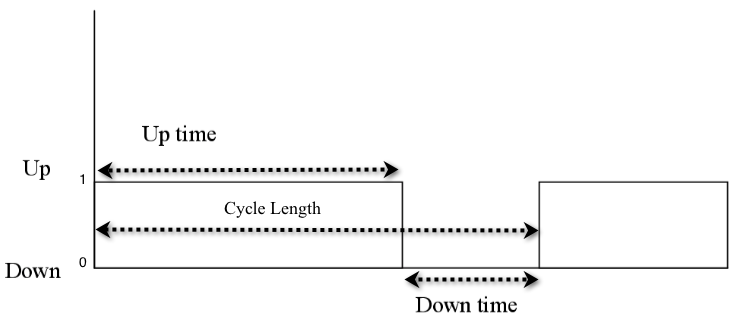
\includegraphics{./figures/ch4/UpDownComponent.png}
\caption{\label{fig:UpDownComponent}Up and Down Component Process}
\end{figure}

Figure \ref{fig:UpDownComponent} illustrates the dynamics of the
component over time.

The following steps are useful in developing this model:

\begin{enumerate}
\def\labelenumi{\arabic{enumi}.}
\tightlist
\item
  Conceptualize the system/objects and their states
\item
  Determine the events and the actions associated with the events
\item
  Determine how to represent the system and objects as ModelElements
\item
  Determine how to initialize and run the model
\end{enumerate}

The first step is to conceptualize how to model the system and the state
of the component. A model element, UpDownComponent, will be used to
model the component. To track the state of the component, it is
necessary to know whether or not the component is UP or DOWN. A variable
can be used to represent this state. However, since we need to estimate
the proportion of time that the component is in the UP state, a
\texttt{TimeWeighted} variable will be used. \texttt{TimeWeighted} is a sub-class of
\texttt{ModelElement} that facilitates the observation and statistical collection
of time-based variables. Time-bases variables, which are discussed
further in the next Chapter, are a type of variable that changes values
at particular instants of time. Time-based variables must have
time-weighted statistics collected. Time-weighted statistics weights the
value of the variable by the proportion of time that the variable is set
to a value. To collect statistics on the cycle length we can use a
\texttt{ResponseVariable}. \texttt{ResponseVariable} is a sub-class of \texttt{ModelElement} that
can take on values within a simulation model and allows easy statistical
observation of its values during the simulation run. This class provides
observation-based statistical collection. Further discussion of
observation-based statistics will be presented in the next Chapter.

Because this system is so simple the required performance measures can
be easily computed theoretically. According to renewal theory, the
probability of being in the UP state in the long run should be equal to:

\[P(UP) = \frac{\theta_{u}}{\theta_{u}+\theta_{d}} = \frac{1.0}{1.0+2.0}=0.\overline{33}\]

where \(\theta_{u}\) is the mean of the up-time distribution and
\(\theta_{d}\) is the mean of the down-time distribution. In addition, the
expected cycle length should be \(\theta_{u}+\theta_{d} = 3.0\).

The \texttt{UpDownComponent} class extends the \texttt{SchedulingElement} class and has
object references to instances of \texttt{RandomVariable}, \texttt{TimeWeighted},
\texttt{ResponseVariable}, and \texttt{Counter} classes. Within the constructor of
\texttt{UpDownComponent}, we need to create the instances of these objects for
use within the class, as shown in the following code fragment.

\begin{Shaded}
\begin{Highlighting}[]
\KeywordTok{public} \KeywordTok{class}\NormalTok{ UpDownComponent }\KeywordTok{extends}\NormalTok{ SchedulingElement }\OperatorTok{\{}

    \KeywordTok{public} \DataTypeTok{static} \DataTypeTok{final} \DataTypeTok{int}\NormalTok{ UP }\OperatorTok{=} \DecValTok{1}\OperatorTok{;}
    \KeywordTok{public} \DataTypeTok{static} \DataTypeTok{final} \DataTypeTok{int}\NormalTok{ DOWN }\OperatorTok{=} \DecValTok{0}\OperatorTok{;}
    \KeywordTok{private}\NormalTok{ RandomVariable myUpTime}\OperatorTok{;}
    \KeywordTok{private}\NormalTok{ RandomVariable myDownTime}\OperatorTok{;}
    \KeywordTok{private}\NormalTok{ TimeWeighted myState}\OperatorTok{;}
    \KeywordTok{private}\NormalTok{ ResponseVariable myCycleLength}\OperatorTok{;}
    \KeywordTok{private}\NormalTok{ Counter myCountFailures}\OperatorTok{;}
    \KeywordTok{private} \DataTypeTok{final}\NormalTok{ UpChangeAction myUpChangeAction }\OperatorTok{=} \KeywordTok{new} \FunctionTok{UpChangeAction}\OperatorTok{();}
    \KeywordTok{private} \DataTypeTok{final}\NormalTok{ DownChangeAction myDownChangeAction }\OperatorTok{=} \KeywordTok{new} \FunctionTok{DownChangeAction}\OperatorTok{();}
    \KeywordTok{private} \DataTypeTok{double}\NormalTok{ myTimeLastUp}\OperatorTok{;}

    \KeywordTok{public} \FunctionTok{UpDownComponent}\OperatorTok{(}\NormalTok{ModelElement parent}\OperatorTok{)} \OperatorTok{\{}
        \KeywordTok{this}\OperatorTok{(}\NormalTok{parent}\OperatorTok{,} \KeywordTok{null}\OperatorTok{);}
    \OperatorTok{\}}

    \KeywordTok{public} \FunctionTok{UpDownComponent}\OperatorTok{(}\NormalTok{ModelElement parent}\OperatorTok{,} \BuiltInTok{String}\NormalTok{ name}\OperatorTok{)} \OperatorTok{\{}
        \KeywordTok{super}\OperatorTok{(}\NormalTok{parent}\OperatorTok{,}\NormalTok{ name}\OperatorTok{);}
\NormalTok{        RVariableIfc utd }\OperatorTok{=} \KeywordTok{new} \FunctionTok{ExponentialRV}\OperatorTok{(}\FloatTok{1.0}\OperatorTok{);}
\NormalTok{        RVariableIfc dtd }\OperatorTok{=} \KeywordTok{new} \FunctionTok{ExponentialRV}\OperatorTok{(}\FloatTok{2.0}\OperatorTok{);}
\NormalTok{        myUpTime }\OperatorTok{=} \KeywordTok{new} \FunctionTok{RandomVariable}\OperatorTok{(}\KeywordTok{this}\OperatorTok{,}\NormalTok{ utd}\OperatorTok{,} \StringTok{"up time"}\OperatorTok{);}
\NormalTok{        myDownTime }\OperatorTok{=} \KeywordTok{new} \FunctionTok{RandomVariable}\OperatorTok{(}\KeywordTok{this}\OperatorTok{,}\NormalTok{ dtd}\OperatorTok{,} \StringTok{"down time"}\OperatorTok{);}
\NormalTok{        myState }\OperatorTok{=} \KeywordTok{new} \FunctionTok{TimeWeighted}\OperatorTok{(}\KeywordTok{this}\OperatorTok{,} \StringTok{"state"}\OperatorTok{);}
\NormalTok{        myCycleLength }\OperatorTok{=} \KeywordTok{new} \FunctionTok{ResponseVariable}\OperatorTok{(}\KeywordTok{this}\OperatorTok{,} \StringTok{"cycle length"}\OperatorTok{);}
\NormalTok{        myCountFailures }\OperatorTok{=} \KeywordTok{new} \FunctionTok{Counter}\OperatorTok{(}\KeywordTok{this}\OperatorTok{,} \StringTok{"count failures"}\OperatorTok{);}
    \OperatorTok{\}}
\end{Highlighting}
\end{Shaded}

Lines~3~and~4 define two constants to represent
the up and down states. Lines~5-9 declare additional references
needed to represent the up and down time random variables and the
variables that need statistical collection (myState, myCycleLength, and
myCountFailures). Lines~10~and~11 define and create the event actions
associated with the end of the up-time and the end of the down time. The
variable \texttt{myTimeLastUp} is used to keep track of the time that the
component last changed into the UP state, which allows the cycle length
to be collected. In lines~20-23, the random variables for the up and
downtime are constructed using exponential distributions.

As show in the following code listing, the \texttt{initialize()} method sets up the component.The variable \texttt{myTimeLastUp} is set to 0.0 in order to assume that the last time the component was in the UP state started at time 0.0. Thus,
we are assuming that the component starts the simulation in the UP
state. Finally, in line~7 the initial event is scheduled to cause the
component to go down according to the uptime distribution. This is the
first event and then the component can start its regular up and down
pattern. In the action associated with the change to the UP state,
line~18 sets the state to UP. Line~22 schedules the time until the
component goes down. Line~16 causes statistics to be collected on the
value of the cycle length. The code \texttt{getTime()-myTimeLastUp} represents
the elapsed time since the value of \texttt{myTimeLastUp} was set (in line~20),
which represents the cycle length. The \texttt{DownChangeAction} is very similar.
Line~31 counts the number of failures (times that the component has gone
down). Line~32 sets the state of the component to DOWN and line~34
schedules when the component should next transition into the UP state.

\begin{Shaded}
\begin{Highlighting}[]
\KeywordTok{public} \DataTypeTok{void} \FunctionTok{initialize}\OperatorTok{()} \OperatorTok{\{}
    \CommentTok{// assume that the component starts in the UP state at time 0.0}
\NormalTok{    myTimeLastUp }\OperatorTok{=} \FloatTok{0.0}\OperatorTok{;}
\NormalTok{    myState}\OperatorTok{.}\FunctionTok{setValue}\OperatorTok{(}\NormalTok{UP}\OperatorTok{);}
    \CommentTok{// schedule the time that it goes down}
    \FunctionTok{scheduleEvent}\OperatorTok{(}\NormalTok{myDownChangeAction}\OperatorTok{,}\NormalTok{ myUpTime}\OperatorTok{.}\FunctionTok{getValue}\OperatorTok{());}
    \CommentTok{//schedule(myDownChangeAction).name("Down").in(myUpTime).units();}
\OperatorTok{\}}

\KeywordTok{private} \KeywordTok{class}\NormalTok{ UpChangeAction }\KeywordTok{extends}\NormalTok{ EventAction }\OperatorTok{\{}

    \AttributeTok{@Override}
    \KeywordTok{public} \DataTypeTok{void} \FunctionTok{action}\OperatorTok{(}\NormalTok{JSLEvent event}\OperatorTok{)} \OperatorTok{\{}
        \CommentTok{// this event action represents what happens when the component goes up}
        \CommentTok{// record the cycle length, the time btw up states}
\NormalTok{        myCycleLength}\OperatorTok{.}\FunctionTok{setValue}\OperatorTok{(}\FunctionTok{getTime}\OperatorTok{()} \OperatorTok{{-}}\NormalTok{ myTimeLastUp}\OperatorTok{);}
        \CommentTok{// component has just gone up, change its state value}
\NormalTok{        myState}\OperatorTok{.}\FunctionTok{setValue}\OperatorTok{(}\NormalTok{UP}\OperatorTok{);}
        \CommentTok{// record the time it went up}
\NormalTok{        myTimeLastUp }\OperatorTok{=} \FunctionTok{getTime}\OperatorTok{();}
        \CommentTok{// schedule the down state change after the uptime}
        \FunctionTok{scheduleEvent}\OperatorTok{(}\NormalTok{myDownChangeAction}\OperatorTok{,}\NormalTok{ myUpTime}\OperatorTok{.}\FunctionTok{getValue}\OperatorTok{());}
    \OperatorTok{\}}
\OperatorTok{\}}

\KeywordTok{private} \KeywordTok{class}\NormalTok{ DownChangeAction }\KeywordTok{extends}\NormalTok{ EventAction }\OperatorTok{\{}

    \AttributeTok{@Override}
    \KeywordTok{public} \DataTypeTok{void} \FunctionTok{action}\OperatorTok{(}\NormalTok{JSLEvent event}\OperatorTok{)} \OperatorTok{\{}
        \CommentTok{// component has just gone down, change its state value}
\NormalTok{        myCountFailures}\OperatorTok{.}\FunctionTok{increment}\OperatorTok{();}
\NormalTok{        myState}\OperatorTok{.}\FunctionTok{setValue}\OperatorTok{(}\NormalTok{DOWN}\OperatorTok{);}
        \CommentTok{// schedule when it goes up afer the down time}
        \FunctionTok{scheduleEvent}\OperatorTok{(}\NormalTok{myUpChangeAction}\OperatorTok{,}\NormalTok{ myDownTime}\OperatorTok{.}\FunctionTok{getValue}\OperatorTok{());}
    \OperatorTok{\}}
\OperatorTok{\}}
\end{Highlighting}
\end{Shaded}

The following listing presents the code to construct and execute the
simulation. This code is very similar to previously presented code for
running a simulation. In line~3, the simulation is constructed. Then, in
line~5, the model associated with the simulation is accessed. This model
is then used to construct an instance of the UpDownComponent in line~7.
Finally, lines~9-15 represent getting a SimulationReporter, running the
simulation, and causing output to be written to the console.

\begin{Shaded}
\begin{Highlighting}[]
\KeywordTok{public} \DataTypeTok{static} \DataTypeTok{void} \FunctionTok{main}\OperatorTok{(}\BuiltInTok{String}\OperatorTok{[]}\NormalTok{ args}\OperatorTok{)} \OperatorTok{\{}
    \CommentTok{// create the simulation}
\NormalTok{    Simulation s }\OperatorTok{=} \KeywordTok{new} \FunctionTok{Simulation}\OperatorTok{(}\StringTok{"UpDownComponent"}\OperatorTok{);}
\NormalTok{    s}\OperatorTok{.}\FunctionTok{turnOnDefaultEventTraceReport}\OperatorTok{();}
\NormalTok{    s}\OperatorTok{.}\FunctionTok{turnOnLogReport}\OperatorTok{();}
    \CommentTok{// get the model associated with the simulation}
\NormalTok{    Model m }\OperatorTok{=}\NormalTok{ s}\OperatorTok{.}\FunctionTok{getModel}\OperatorTok{();}
    \CommentTok{// create the model element and attach it to the model}
\NormalTok{    UpDownComponent tv }\OperatorTok{=} \KeywordTok{new} \FunctionTok{UpDownComponent}\OperatorTok{(}\NormalTok{m}\OperatorTok{);}
    \CommentTok{// make the simulation reporter}
\NormalTok{    SimulationReporter r }\OperatorTok{=}\NormalTok{ s}\OperatorTok{.}\FunctionTok{makeSimulationReporter}\OperatorTok{();}
    \CommentTok{// set the running parameters of the simulation}
\NormalTok{    s}\OperatorTok{.}\FunctionTok{setNumberOfReplications}\OperatorTok{(}\DecValTok{5}\OperatorTok{);}
\NormalTok{    s}\OperatorTok{.}\FunctionTok{setLengthOfReplication}\OperatorTok{(}\FloatTok{5000.0}\OperatorTok{);}
    \CommentTok{// tell the simulation to run}
\NormalTok{    s}\OperatorTok{.}\FunctionTok{run}\OperatorTok{();}
\NormalTok{    r}\OperatorTok{.}\FunctionTok{printAcrossReplicationSummaryStatistics}\OperatorTok{();}
\OperatorTok{\}}
\end{Highlighting}
\end{Shaded}

The results for the average time in the up state and the cycle length are consistent
with the theoretically computed results.

\begin{verbatim}
---------------------------------------------------------
Across Replication Statistical Summary Report
Sat Dec 31 18:31:27 EST 2016
Simulation Results for Model: UpDownComponent_Model

Number of Replications: 30
Length of Warm up period: 0.0
Length of Replications: 5000.0
---------------------------------------------------------
Response Variables
---------------------------------------------------------
Name              Average       Std. Dev.       Count 
---------------------------------------------------------
state             0.335537       0.005846       30.000000 
cycle length      2.994080       0.040394       30.000000 
---------------------------------------------------------

---------------------------------------------------------
Counters
---------------------------------------------------------
Name             Average        Std. Dev.    Count 
---------------------------------------------------------
count failures   1670.066667    22.996152    30.000000 
---------------------------------------------------------
\end{verbatim}

This example only scratches the surface of what is possible. Imagine if
there were 20 components. We could easily create 20 of instances and add
them to the model. Even more interesting would be to define the state of
the system based on which components were in the up state. This would be
the beginning of modeling the reliability of a complex system. This type
of modeling can be achieved by making the individual model elements
(e.g.~\texttt{UpDownComponent}) more reusable and allow the modeling objects to
interact in complex ways. More complex modeling will be the focus of the
next chapter.

\hypertarget{introDEDS:pharmacy}{%
\subsection{Modeling a Simple Queueing System}\label{introDEDS:pharmacy}}

This example considers a small pharmacy that has a single line for
waiting customers and only one pharmacist. Assume that customers arrive
at a drive through pharmacy window according to a Poisson distribution
with a mean of 10 per hour. The time that it takes the pharmacist to
serve the customer is random and data has indicated that the time is
well modeled with an exponential distribution with a mean of 3 minutes.
Customers who arrive to the pharmacy are served in the order of arrival
and enough space is available within the parking area of the adjacent
grocery store to accommodate any waiting customers.

\begin{figure}
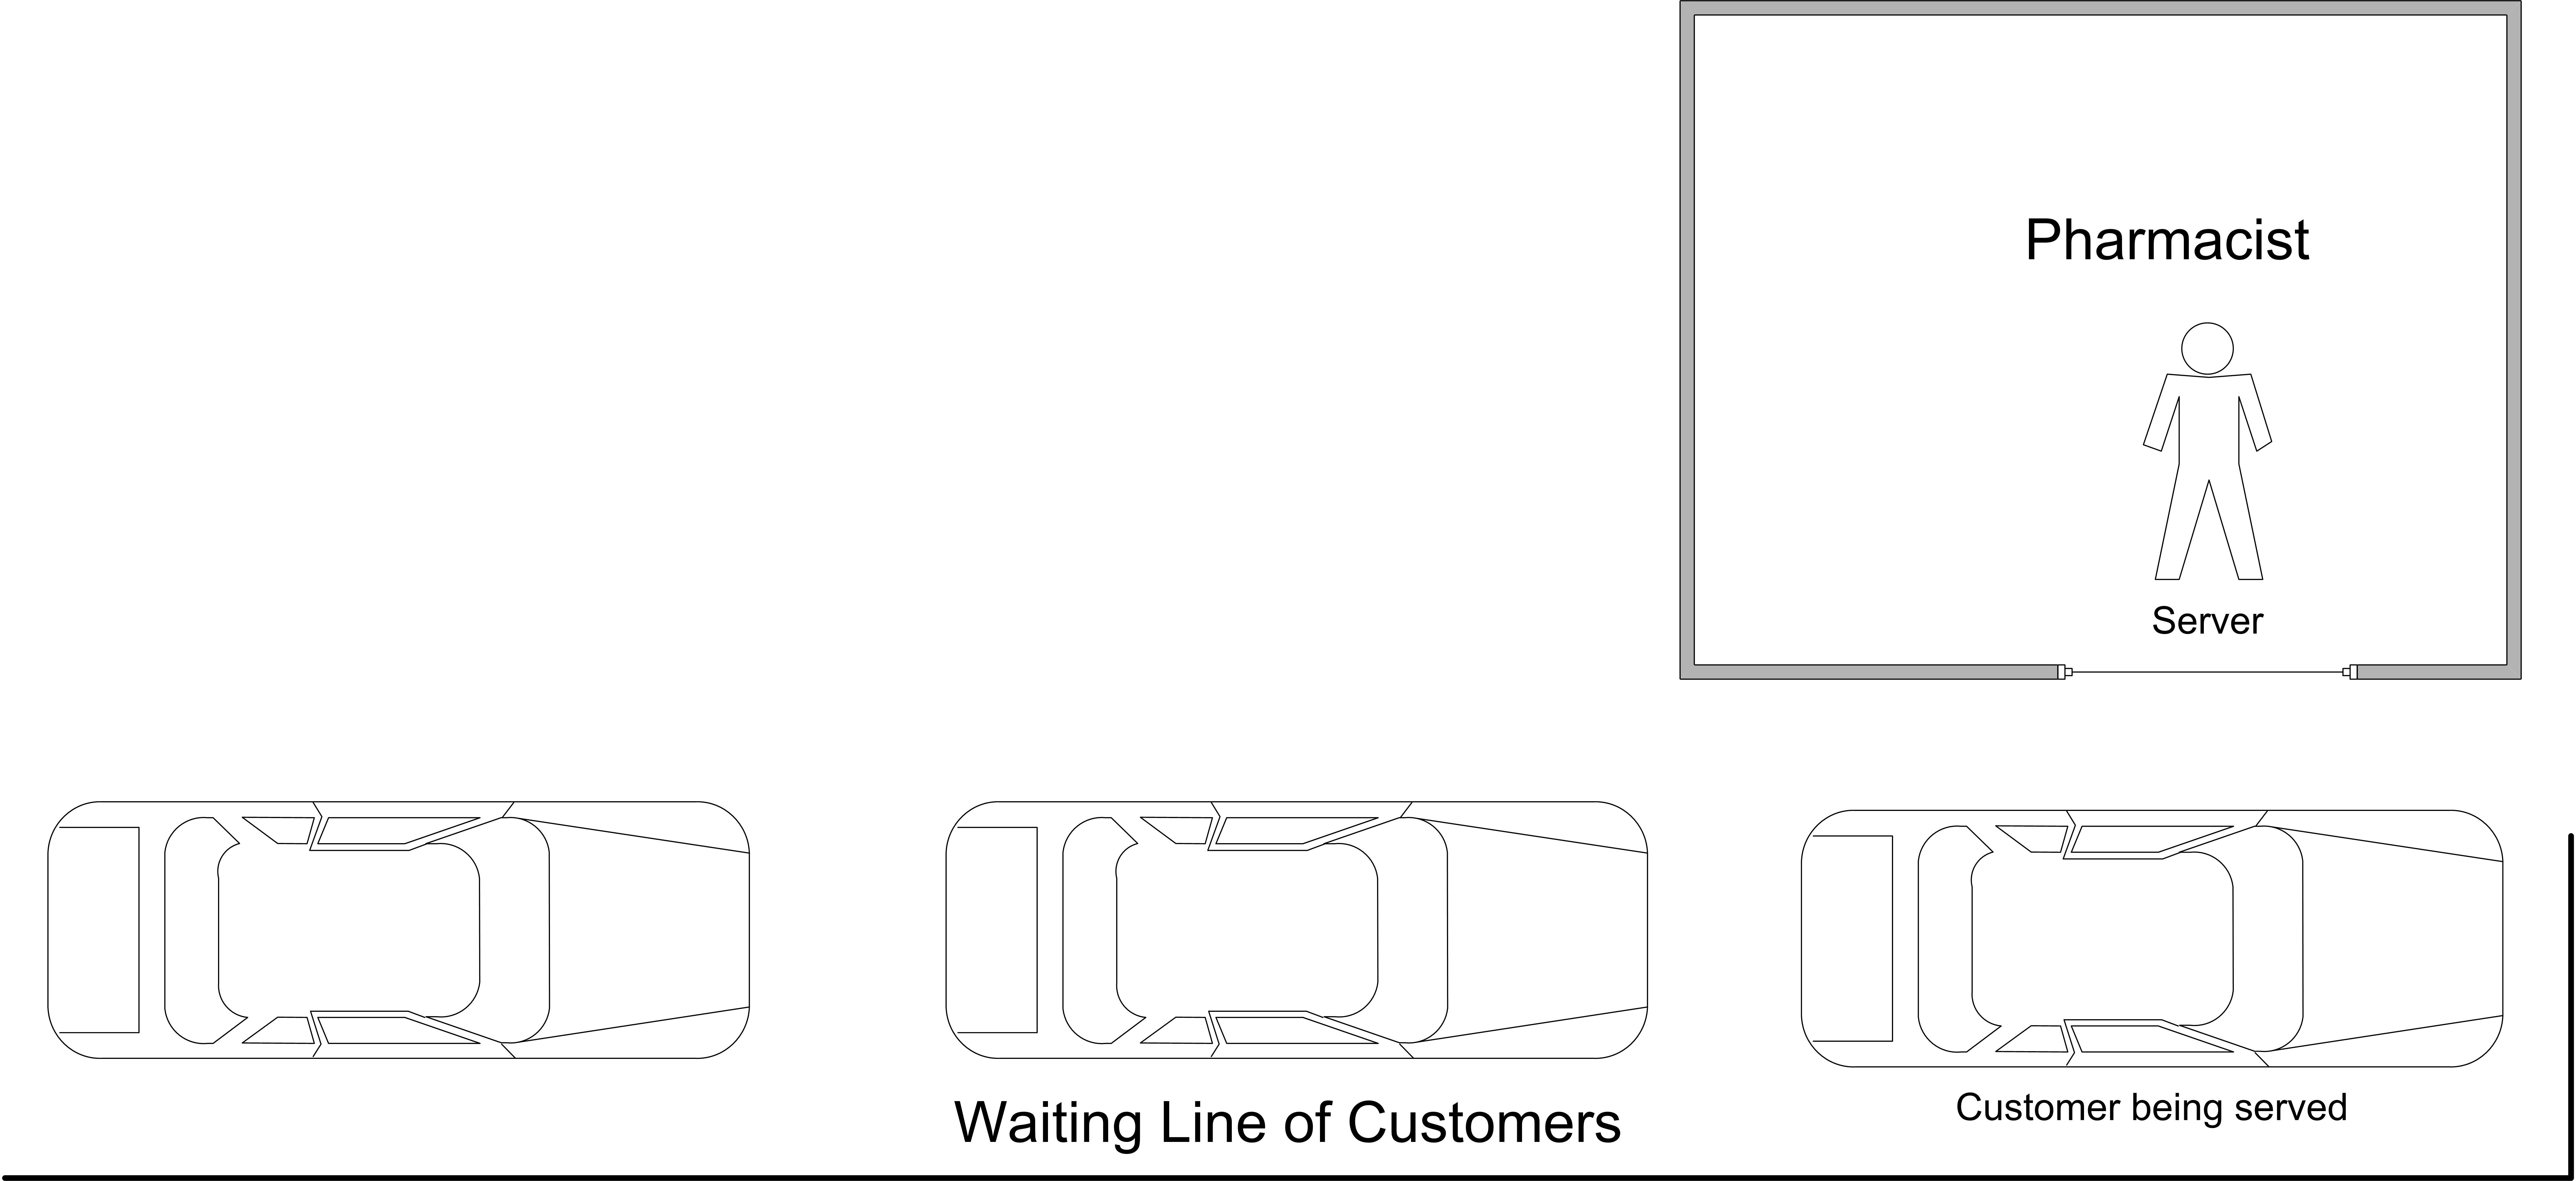
\includegraphics[width=0.8\linewidth,height=0.8\textheight]{./figures/ch4/ch4fig8} \caption{Drive Through Pharmacy}\label{fig:DriveThruPharmacy}
\end{figure}

The drive through pharmacy system can be conceptualized as a single
server waiting line system, where the server is the pharmacist. An
idealized representation of this system is shown in Figure \ref{fig:DriveThruPharmacy}. If the pharmacist is busy serving a
customer, then additional customers will wait in line. In such a
situation, management might be interested in how long customers wait in
line, before being served by the pharmacist. In addition, management
might want to predict if the number of waiting cars will be large.
Finally, they might want to estimate the utilization of the pharmacist
in order to ensure that he or she is not too busy.

When modeling the system first question to ask is: \emph{What is the system}?
In this situation, the system is the pharmacist and the potential
customers as idealized in Figure \ref{fig:DriveThruPharmacy}. Now you should consider the entities of
the system. An entity is a conceptual thing of importance that flows
through a system potentially using the resources of the system.
Therefore, one of the first questions to ask when developing a model is:
\emph{What are the entities}? In this situation, the entities are the
customers that need to use the pharmacy. This is because customers are
discrete things that enter the system, flow through the system, and then
depart the system.

Since entities often use things as they flow through the system, a
natural question is to ask: \emph{What are the resources that are used by the
entities}? A resource is something that is used by the entities and that
may constrain the flow of the entities within the system. Another way to
think of resources is to think of the things that provide service in the
system. In this situation, the entities ``use'' the pharmacist in order to
get their medicine. Thus, the pharmacist is a resource.

Another useful conceptual modeling tool is the \emph{activity diagram}. An
\emph{activity} is an operation that takes time to complete. An activity is
associated with the state of an object over an interval of time.
Activities are defined by the occurrence of two events which represent
the activity's beginning time and ending time and mark the entrance and
exit of the state associated with the activity. An activity diagram is a
pictorial representation of the process (steps of activities) for an
entity and its interaction with resources while within the system. If
the entity is a temporary entity (i.e.~it flows through the system) the
activity diagram is called an activity flow diagram. If the entity is
permanent (i.e.~it remains in the system throughout its life) the
activity diagram is called an activity cycle diagram. The notation of an
activity diagram is very simple, and can be augmented as needed to
explain additional concepts:

Queues: shown as a circle with queue labeled inside

Activities: shown as a rectangle with appropriate label inside

Resources: shown as small circles with resource labeled inside

Lines/arcs: indicating flow (precedence ordering) for engagement of entities in
activities or for obtaining resources. Dotted lines are used to
indicate the seizing and releasing of resources.

zigzag lines: indicate the creation or destruction of entities

Activity diagrams are especially useful for illustrating how entities
interact with resources. In addition, activity diagrams help in finding
the events and in identifying some the state changes that must be
modeled. Activity diagrams are easy to build by hand and serve as a
useful communication mechanism. Since they have a simple set of symbols,
it is easy to use an activity diagram to communicate with people who
have little simulation background. Activity diagrams are an excellent
mechanism to document a conceptual model of the system before building
the model.

\begin{figure}
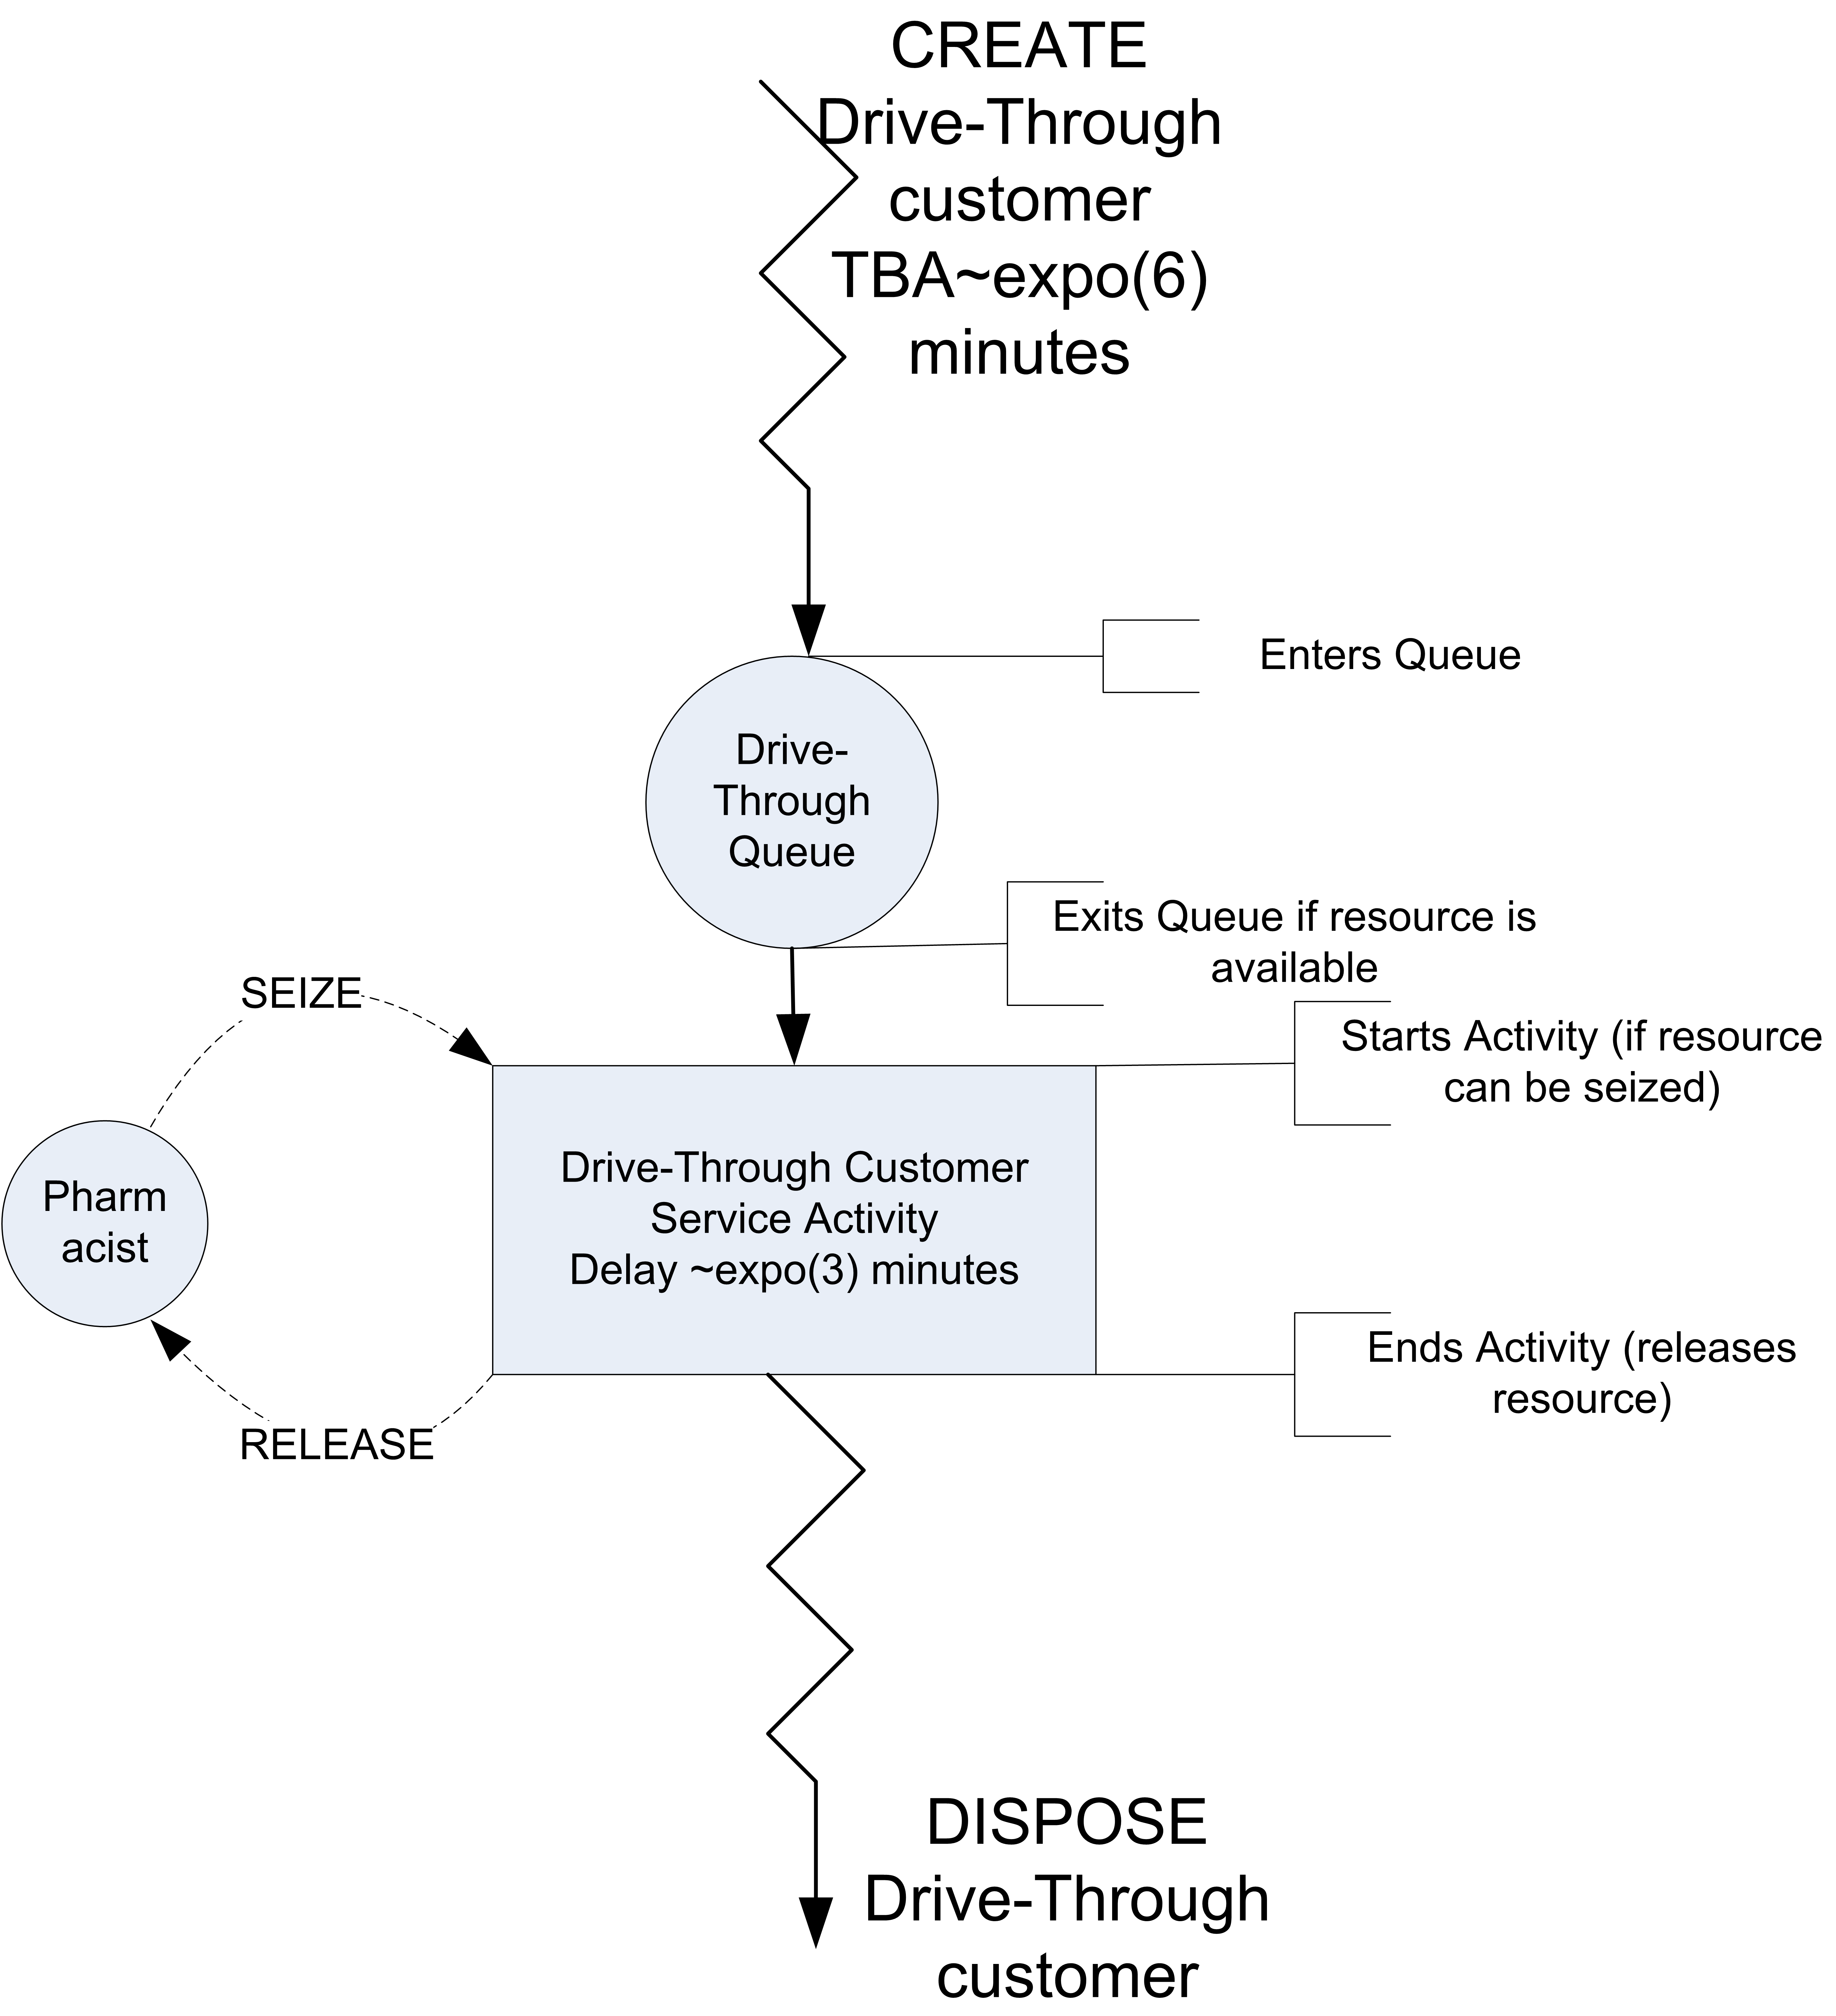
\includegraphics[width=0.8\linewidth,height=0.8\textheight]{./figures/ch4/ch4fig9} \caption{Activity Diagram of Drive through Pharmacy}\label{fig:DTPActivityDiagram}
\end{figure}

Figure \ref{fig:DTPActivityDiagram} shows the activity diagram for the
pharmacy situation. The diagram describes the life of an entity within
the system. The zigzag lines at the top of the diagram indicate the
creation of an entity. Consider following the life of the customer
through the pharmacy. Following the direction of the arrows, the
customers are first created and then enter the queue. Notice that the
diagram clearly shows that there is a queue for the drive-through
customers. You should think of the entity flowing through the diagram.
As it flows through the queue, the customer attempts to start an
activity. In this case, the activity requires a resource. The pharmacist
is shown as a resource (circle) next to the rectangle that represents
the service activity.

The customer requires the resource in order to start its service
activity. This is indicated by the dashed arrow from the pharmacist
(resource) to the top of the service activity rectangle. If the customer
does not get the resource, they wait in the queue. Once they receive the
number of units of the resource requested, they proceed with the
activity. The activity represents a delay of time and in this case the
resource is used throughout the delay. After the activity is completed,
the customer releases the pharmacist (resource). This is indicated by
another dashed arrow, with the direction indicating that the units of the resource aare
being put back or released. After the customer completes its service
activity, the customer leaves the system. This is indicated with the
zigzag lines going to no-where and indicating that the object leaves the
system and is disposed The conceptual model of this system can be
summarized as follows:

System: The system has a pharmacist that acts as a resource, customers that
act as entities, and a queue to hold the waiting customers. The
state of the system includes the number of customers in the system,
in the queue, and in service.

Events: Arrivals of customers to the system, which occur within an
inter-event time that is exponentially distributed with a mean of 6
minutes.

Activities: The service time of the customers are exponentially distributed with
a mean of 3 minutes.

Conditional delays: A conditional delay occurs when an entity has to wait for a
condition to occur in order to proceed. In this system, the customer
may have to wait in a queue until the pharmacist becomes available.

With an activity diagram and pseudo-code such as this available to
represent a solid conceptual understanding of the system, you can begin
the model development process.

In the current example, pharmacy customers arrive according to a Poisson
process with a mean of \(\lambda\) = 10 per hour. According to probability
theory, this implies that the time between arrivals is exponentially
distributed with a mean of (1/\(\lambda\)). Thus, for this situation, the
mean time between arrivals is 6 minutes.

\[\frac{1}{\lambda} = \frac{\text{1 hour}}{\text{10 customers}} \times \frac{\text{60 minutes}}{\text{1 hour}} = \frac{\text{6 minutes}}{\text{customers}}\]

Let's assume that the pharmacy is open 24 hours a day, 7 days a week. In
other words, it is always open. In addition, assume that the arrival
process does not vary with respect to time. Finally, assume that
management is interested in understanding the long term behavior of this
system in terms of the average waiting time of customers, the average
number of customers, and the utilization of the pharmacist.

To simulate this situation over time, you must specify how long to run
the model. Ideally, since management is interested in long run
performance, you should run the model for an infinite amount of time to
get long term performance; however, you probably don't want to wait that
long! For the sake of simplicity, assume that 10,000 hours of operation
is long enough.

The logic of this model follows very closely the discussion of the bank
teller example. The following code listing presents the definition of the variables and their creation.

\begin{Shaded}
\begin{Highlighting}[]
\KeywordTok{public} \KeywordTok{class}\NormalTok{ DriveThroughPharmacy }\KeywordTok{extends}\NormalTok{ SchedulingElement }\OperatorTok{\{}

    \KeywordTok{private} \DataTypeTok{int}\NormalTok{ myNumPharmacists}\OperatorTok{;}
    \KeywordTok{private} \BuiltInTok{Queue}\OperatorTok{\textless{}}\NormalTok{QObject}\OperatorTok{\textgreater{}}\NormalTok{ myWaitingQ}\OperatorTok{;}
    \KeywordTok{private}\NormalTok{ RandomIfc myServiceRS}\OperatorTok{;}
    \KeywordTok{private}\NormalTok{ RandomIfc myArrivalRS}\OperatorTok{;}
    \KeywordTok{private}\NormalTok{ RandomVariable myServiceRV}\OperatorTok{;}
    \KeywordTok{private}\NormalTok{ RandomVariable myArrivalRV}\OperatorTok{;}
    \KeywordTok{private}\NormalTok{ TimeWeighted myNumBusy}\OperatorTok{;}
    \KeywordTok{private}\NormalTok{ TimeWeighted myNS}\OperatorTok{;}
    \KeywordTok{private}\NormalTok{ ResponseVariable mySysTime}\OperatorTok{;}
    \KeywordTok{private}\NormalTok{ ArrivalEventAction myArrivalEventAction}\OperatorTok{;}
    \KeywordTok{private}\NormalTok{ EndServiceEventAction myEndServiceEventAction}\OperatorTok{;}
    \KeywordTok{private}\NormalTok{ Counter myNumCustomers}\OperatorTok{;}

    \KeywordTok{public} \FunctionTok{DriveThroughPharmacy}\OperatorTok{(}\NormalTok{ModelElement parent}\OperatorTok{)} \OperatorTok{\{}
        \KeywordTok{this}\OperatorTok{(}\NormalTok{parent}\OperatorTok{,} \DecValTok{1}\OperatorTok{,}
                \KeywordTok{new} \FunctionTok{ExponentialRV}\OperatorTok{(}\FloatTok{1.0}\OperatorTok{),} \KeywordTok{new} \FunctionTok{ExponentialRV}\OperatorTok{(}\FloatTok{0.5}\OperatorTok{));}
    \OperatorTok{\}}

    \KeywordTok{public} \FunctionTok{DriveThroughPharmacy}\OperatorTok{(}\NormalTok{ModelElement parent}\OperatorTok{,} \DataTypeTok{int}\NormalTok{ numServers}\OperatorTok{)} \OperatorTok{\{}
        \KeywordTok{this}\OperatorTok{(}\NormalTok{parent}\OperatorTok{,}\NormalTok{ numServers}\OperatorTok{,} \KeywordTok{new} \FunctionTok{ExponentialRV}\OperatorTok{(}\FloatTok{1.0}\OperatorTok{),} \KeywordTok{new} \FunctionTok{ExponentialRV}\OperatorTok{(}\FloatTok{0.5}\OperatorTok{));}
    \OperatorTok{\}}

    \KeywordTok{public} \FunctionTok{DriveThroughPharmacy}\OperatorTok{(}\NormalTok{ModelElement parent}\OperatorTok{,} \DataTypeTok{int}\NormalTok{ numServers}\OperatorTok{,}\NormalTok{ RandomIfc ad}\OperatorTok{,}\NormalTok{ RandomIfc sd}\OperatorTok{)} \OperatorTok{\{}
        \KeywordTok{super}\OperatorTok{(}\NormalTok{parent}\OperatorTok{);}
        \FunctionTok{setNumberOfPharmacists}\OperatorTok{(}\NormalTok{numServers}\OperatorTok{);}
        \FunctionTok{setServiceRS}\OperatorTok{(}\NormalTok{sd}\OperatorTok{);}
        \FunctionTok{setArrivalRS}\OperatorTok{(}\NormalTok{ad}\OperatorTok{);}
\NormalTok{        myWaitingQ }\OperatorTok{=} \KeywordTok{new} \BuiltInTok{Queue}\OperatorTok{\textless{}\textgreater{}(}\KeywordTok{this}\OperatorTok{,} \StringTok{"PharmacyQ"}\OperatorTok{);}
\NormalTok{        myNumBusy }\OperatorTok{=} \KeywordTok{new} \FunctionTok{TimeWeighted}\OperatorTok{(}\KeywordTok{this}\OperatorTok{,} \FloatTok{0.0}\OperatorTok{,} \StringTok{"NumBusy"}\OperatorTok{);}
\NormalTok{        myNS }\OperatorTok{=} \KeywordTok{new} \FunctionTok{TimeWeighted}\OperatorTok{(}\KeywordTok{this}\OperatorTok{,} \FloatTok{0.0}\OperatorTok{,} \StringTok{"\# in System"}\OperatorTok{);}
\NormalTok{        mySysTime }\OperatorTok{=} \KeywordTok{new} \FunctionTok{ResponseVariable}\OperatorTok{(}\KeywordTok{this}\OperatorTok{,} \StringTok{"System Time"}\OperatorTok{);}
\NormalTok{        myNumCustomers }\OperatorTok{=} \KeywordTok{new} \FunctionTok{Counter}\OperatorTok{(}\KeywordTok{this}\OperatorTok{,} \StringTok{"Num Served"}\OperatorTok{);}
\NormalTok{        myArrivalEventAction }\OperatorTok{=} \KeywordTok{new} \FunctionTok{ArrivalEventAction}\OperatorTok{();}
\NormalTok{        myEndServiceEventAction }\OperatorTok{=} \KeywordTok{new} \FunctionTok{EndServiceEventAction}\OperatorTok{();}
    \OperatorTok{\}}
\end{Highlighting}
\end{Shaded}

The \texttt{RandomVariable} class is used to model the time between
arrivals and the service time random variables. The \texttt{TimeWeighted} class
is used to model the number of busy servers and the number of customers
in the system. A \texttt{ResponseVariable} is used to model the time spent in the
system. There are two events represented by implementing the
\texttt{EventActionIfc} interface to model the arrival event and the end of
service event. Finally, a new JSL class, the \texttt{Queue} class, is used to
model the waiting line within the system. The \texttt{Queue} class is a sub-class
of \texttt{ModelElement} that is able to hold instances of the class \texttt{QObject} and
will automatically collect statistics on the number in the queue and the
time spent in the queue. The following code listing shows the logic required to model the
arrivals to the pharmacy.

\begin{Shaded}
\begin{Highlighting}[]
    \KeywordTok{protected} \DataTypeTok{void} \FunctionTok{initialize}\OperatorTok{()} \OperatorTok{\{}
        \KeywordTok{super}\OperatorTok{.}\FunctionTok{initialize}\OperatorTok{();}
        \CommentTok{// start the arrivals}
        \FunctionTok{scheduleEvent}\OperatorTok{(}\NormalTok{myArrivalEventAction}\OperatorTok{,}\NormalTok{ myArrivalRV}\OperatorTok{);}
    \OperatorTok{\}}

    \KeywordTok{private} \KeywordTok{class}\NormalTok{ ArrivalEventAction }\KeywordTok{extends}\NormalTok{ EventAction }\OperatorTok{\{}
        \AttributeTok{@Override}
        \KeywordTok{public} \DataTypeTok{void} \FunctionTok{action}\OperatorTok{(}\NormalTok{JSLEvent event}\OperatorTok{)} \OperatorTok{\{}
            \CommentTok{//   schedule the next arrival}
            \FunctionTok{scheduleEvent}\OperatorTok{(}\NormalTok{myArrivalEventAction}\OperatorTok{,}\NormalTok{ myArrivalRV}\OperatorTok{);}
            \FunctionTok{enterSystem}\OperatorTok{();}
        \OperatorTok{\}}
    \OperatorTok{\}}

    \KeywordTok{private} \DataTypeTok{void} \FunctionTok{enterSystem}\OperatorTok{()} \OperatorTok{\{}
\NormalTok{        myNS}\OperatorTok{.}\FunctionTok{increment}\OperatorTok{();} \CommentTok{// new customer arrived}
\NormalTok{        QObject arrivingCustomer }\OperatorTok{=} \KeywordTok{new} \FunctionTok{QObject}\OperatorTok{(}\FunctionTok{getTime}\OperatorTok{());}

\NormalTok{        myWaitingQ}\OperatorTok{.}\FunctionTok{enqueue}\OperatorTok{(}\NormalTok{arrivingCustomer}\OperatorTok{);} \CommentTok{// enqueue the newly arriving customer}
        \ControlFlowTok{if} \OperatorTok{(}\NormalTok{myNumBusy}\OperatorTok{.}\FunctionTok{getValue}\OperatorTok{()} \OperatorTok{\textless{}}\NormalTok{ myNumPharmacists}\OperatorTok{)} \OperatorTok{\{} \CommentTok{// server available}
\NormalTok{            myNumBusy}\OperatorTok{.}\FunctionTok{increment}\OperatorTok{();} \CommentTok{// make server busy}
\NormalTok{            QObject customer }\OperatorTok{=}\NormalTok{ myWaitingQ}\OperatorTok{.}\FunctionTok{removeNext}\OperatorTok{();} \CommentTok{//remove the next customer}
            \CommentTok{// schedule end of service, include the customer as the event\textquotesingle{}s message}
            \FunctionTok{scheduleEvent}\OperatorTok{(}\NormalTok{myEndServiceEventAction}\OperatorTok{,}\NormalTok{ myServiceRV}\OperatorTok{,}\NormalTok{ customer}\OperatorTok{);}
        \OperatorTok{\}}
    \OperatorTok{\}}
\end{Highlighting}
\end{Shaded}

In line~4 the first arrival event is scheduled
within the \texttt{initialize()} method. The \texttt{ArrivalEventAction} implementation
schedules the next arrival using the time between arrival random
variable and calls a private method named \texttt{enterSystem()}. This method
handles the logic for when a customer enters the system. First, the
number in the system is incremented and then the customer is enqueued.
In line~17, an instance of a \texttt{QObject} is created and its creation time is
supplied as the current simulation time using \texttt{getTime()}. Then, the
instance of the \texttt{Queue} class, \texttt{myWaitingQ}, is used to place the customer
in the queue using the \texttt{enqueue()} method. Note that even if the customer
receives immediate service, we still need to place the customer in the
queue because we need to correctly record that there was a zero wait
time. In lines~19-24, the number of busy servers is checked againts the
number of pharmacists. If a server is available, then the server is made
busy, the customer is removed from the queue, and the end of service for
the customer is scheduled. The scheduling of the end of service is
particularly important to note. In line~23, the reference to the \texttt{QObject}
is supplied when calling the \texttt{scheduleEvent()} method. This method has
signature:

\begin{Shaded}
\begin{Highlighting}[]
    \CommentTok{/**}\NormalTok{ Creates an event and schedules it onto the event calendar}
\CommentTok{     * @}\NormalTok{param }\KeywordTok{\textless{}T\textgreater{}}\NormalTok{ the type associated with the attached message}
     \CommentTok{*} \CommentTok{@}\NormalTok{param action represents an ActionListener that will handle the change of state logic}
     \CommentTok{*} \CommentTok{@}\NormalTok{param time represents the inter}\CommentTok{{-}}\NormalTok{event time}\CommentTok{,}\NormalTok{ i}\CommentTok{.}\NormalTok{e}\CommentTok{.}\NormalTok{ the interval from the current time to when the}
     \CommentTok{*}\NormalTok{        event will need to occur}
     \CommentTok{*} \CommentTok{@}\NormalTok{param message is a generic Object that may represent data to be transmitted with the event}
     \CommentTok{*} \CommentTok{@}\NormalTok{return a valid JSLEvent}
     \CommentTok{*/}
    \KeywordTok{protected} \DataTypeTok{final} \OperatorTok{\textless{}}\NormalTok{T}\OperatorTok{\textgreater{}}\NormalTok{ JSLEvent}\OperatorTok{\textless{}}\NormalTok{T}\OperatorTok{\textgreater{}} \FunctionTok{scheduleEvent}\OperatorTok{(}\NormalTok{EventActionIfc}\OperatorTok{\textless{}}\NormalTok{T}\OperatorTok{\textgreater{}}\NormalTok{ action}\OperatorTok{,}\NormalTok{ GetValueIfc time}\OperatorTok{,}\NormalTok{ T message}\OperatorTok{)} \OperatorTok{\{}
        \ControlFlowTok{return} \OperatorTok{(}\FunctionTok{scheduleEvent}\OperatorTok{(}\NormalTok{action}\OperatorTok{,}\NormalTok{ time}\OperatorTok{.}\FunctionTok{getValue}\OperatorTok{(),}\NormalTok{ JSLEvent}\OperatorTok{.}\FunctionTok{DEFAULT\_PRIORITY}\OperatorTok{,}\NormalTok{ message}\OperatorTok{,} \FunctionTok{getName}\OperatorTok{()));}
    \OperatorTok{\}}
\end{Highlighting}
\end{Shaded}

Notice that the last argument of the method is of type \texttt{T}, which is defined as a generic parameter for the method. Thus, using this method, any instance of any class can be supplied.
Notice also that the \texttt{GetValueIfc} interface is used to supply the time.
This is why just the name of the service time random variable can be
used. The method automatically called the \texttt{getValue()} method of the
argument in order to determine the time until the event's occurrence.

The following code fragment presents the logic associated with the end
of service event.

\begin{Shaded}
\begin{Highlighting}[]
    \KeywordTok{private} \KeywordTok{class}\NormalTok{ EndServiceEventAction }\KeywordTok{implements}\NormalTok{ EventActionIfc}\OperatorTok{\textless{}}\NormalTok{QObject}\OperatorTok{\textgreater{}} \OperatorTok{\{}

        \AttributeTok{@Override}
        \KeywordTok{public} \DataTypeTok{void} \FunctionTok{action}\OperatorTok{(}\NormalTok{JSLEvent}\OperatorTok{\textless{}}\NormalTok{QObject}\OperatorTok{\textgreater{}}\NormalTok{ event}\OperatorTok{)} \OperatorTok{\{}
\NormalTok{            myNumBusy}\OperatorTok{.}\FunctionTok{decrement}\OperatorTok{();} \CommentTok{// customer is leaving server is freed}
            \ControlFlowTok{if} \OperatorTok{(!}\NormalTok{myWaitingQ}\OperatorTok{.}\FunctionTok{isEmpty}\OperatorTok{())} \OperatorTok{\{} \CommentTok{// queue is not empty}
\NormalTok{                QObject customer }\OperatorTok{=}\NormalTok{ myWaitingQ}\OperatorTok{.}\FunctionTok{removeNext}\OperatorTok{();} \CommentTok{//remove the next customer}
\NormalTok{                myNumBusy}\OperatorTok{.}\FunctionTok{increment}\OperatorTok{();} \CommentTok{// make server busy}
                \CommentTok{// schedule end of service}
                \FunctionTok{scheduleEvent}\OperatorTok{(}\NormalTok{myEndServiceEventAction}\OperatorTok{,}\NormalTok{ myServiceRV}\OperatorTok{,}\NormalTok{ customer}\OperatorTok{);}
            \OperatorTok{\}}
            \FunctionTok{departSystem}\OperatorTok{(}\NormalTok{event}\OperatorTok{.}\FunctionTok{getMessage}\OperatorTok{());}
        \OperatorTok{\}}
    \OperatorTok{\}}

    \KeywordTok{private} \DataTypeTok{void} \FunctionTok{departSystem}\OperatorTok{(}\NormalTok{QObject departingCustomer}\OperatorTok{)} \OperatorTok{\{}
\NormalTok{        mySysTime}\OperatorTok{.}\FunctionTok{setValue}\OperatorTok{(}\FunctionTok{getTime}\OperatorTok{()} \OperatorTok{{-}}\NormalTok{ departingCustomer}\OperatorTok{.}\FunctionTok{getCreateTime}\OperatorTok{());}
\NormalTok{        myNS}\OperatorTok{.}\FunctionTok{decrement}\OperatorTok{();} \CommentTok{// customer left system}
\NormalTok{        myNumCustomers}\OperatorTok{.}\FunctionTok{increment}\OperatorTok{();}
    \OperatorTok{\}}
\end{Highlighting}
\end{Shaded}

First the number of busy servers is decremented
because the service is becoming idle. Then, the queue is
checked to see if it is not empty. If the queue is not empty, then the
next customer must be removed, the server made busy again
and the customer scheduled into service. Finally, the
private method, \texttt{departSystem()} is called. The argument to this method is
\texttt{event.getMessage()}. The \texttt{getMessage()} method of \texttt{JSLEvent} will
return the object that was scheduled with the event. Since the \texttt{JSLEvent} was provided a \texttt{QObject} for the generic type in the signature of the \texttt{action()} method, we do not need to cast this object to type \texttt{QObject.} The \texttt{departSystem()} method simply collects
statistics using the \texttt{ResponseVariable}, \texttt{mySysTime} and the \texttt{TimeWeighted},
\texttt{myNS.} These objects represent the system time and the number in the
system, respectively.

The following method can be used to run the model based on a desired number of servers.

\begin{Shaded}
\begin{Highlighting}[]
    \KeywordTok{public} \DataTypeTok{static} \DataTypeTok{void} \FunctionTok{runModel}\OperatorTok{(}\DataTypeTok{int}\NormalTok{ numServers}\OperatorTok{)} \OperatorTok{\{}
\NormalTok{        Simulation sim }\OperatorTok{=} \KeywordTok{new} \FunctionTok{Simulation}\OperatorTok{(}\StringTok{"Drive Through Pharmacy"}\OperatorTok{);}
\NormalTok{        sim}\OperatorTok{.}\FunctionTok{setNumberOfReplications}\OperatorTok{(}\DecValTok{30}\OperatorTok{);}
\NormalTok{        sim}\OperatorTok{.}\FunctionTok{setLengthOfReplication}\OperatorTok{(}\FloatTok{20000.0}\OperatorTok{);}
\NormalTok{        sim}\OperatorTok{.}\FunctionTok{setLengthOfWarmUp}\OperatorTok{(}\FloatTok{5000.0}\OperatorTok{);}
        \CommentTok{// add DriveThroughPharmacy to the main model}
\NormalTok{        DriveThroughPharmacy dtp }\OperatorTok{=} \KeywordTok{new} \FunctionTok{DriveThroughPharmacy}\OperatorTok{(}\NormalTok{sim}\OperatorTok{.}\FunctionTok{getModel}\OperatorTok{(),}\NormalTok{ numServers}\OperatorTok{);}
\NormalTok{        dtp}\OperatorTok{.}\FunctionTok{setArrivalRS}\OperatorTok{(}\KeywordTok{new} \FunctionTok{ExponentialRV}\OperatorTok{(}\FloatTok{6.0}\OperatorTok{));}
\NormalTok{        dtp}\OperatorTok{.}\FunctionTok{setServiceRS}\OperatorTok{(}\KeywordTok{new} \FunctionTok{ExponentialRV}\OperatorTok{(}\FloatTok{3.0}\OperatorTok{));}

\NormalTok{        sim}\OperatorTok{.}\FunctionTok{run}\OperatorTok{();}
\NormalTok{        sim}\OperatorTok{.}\FunctionTok{printHalfWidthSummaryReport}\OperatorTok{();}
    \OperatorTok{\}}
\end{Highlighting}
\end{Shaded}

The reports indicate that customers wait about 3 minutes on average in
the line. The utilization of the pharmacist is about 50\%. This means
that about 50\% of the time the pharmacist was busy. For this type of
system, this is probably not a bad utilization, considering that the
pharmacist probably has other in-store duties. The reports also indicate
that there was less than one customer on average waiting for service.

\begin{verbatim}
Across Replication Statistical Summary Report
Mon Jan 02 16:05:23 CST 2017
Simulation Results for Model: Drive Through Pharmacy_Model


Number of Replications: 30
Length of Warm up period: 5000.0
Length of Replications: 20000.0
-------------------------------------------------------------------------------
Response Variables
-------------------------------------------------------------------------------
Name                                  Average       Std. Dev.    Count 
-------------------------------------------------------------------------------
PharmacyQ : Number In Q              0.490898        0.065510       30.000000 
PharmacyQ : Time In Q                2.960012        0.351724       30.000000 
NumBusy                              0.495274        0.016848       30.000000 
# in System                          0.986173        0.080988       30.000000 
System Time                          5.950288        0.403270       30.000000 
-------------------------------------------------------------------------------
\end{verbatim}

This single server waiting line system is a very common situation in
practice. In fact, this exact situation has been studied mathematically
through a branch of operations research called queuing theory. For
specific modeling situations, formulas for the long term performance of
queuing systems can be derived. This particular pharmacy model happens
to be an example of an M/M/1 queuing model. The first M stands for
Markov arrivals, the second M stands for Markov service times, and the 1
represents a single server. Markov was a famous mathematician who
examined the exponential distribution and its properties. According to
queuing theory, the expected number of customer in queue, \(L_q\), for the
M/M/1 model is:

\[
\begin{aligned}
\label{ch4:eq:mm1}
L_q & = \dfrac{\rho^2}{1 - \rho} \\
\rho & = \lambda/\mu \\
\lambda & = \text{arrival rate to queue} \\
\mu & = \text{service rate}
\end{aligned}
\]

In addition, the expected waiting time in queue is given by
\(W_q = L_q/\lambda\). In the pharmacy model, \(\lambda\) = 1/6, i.e.~1
customer every 6 minutes on average, and \(\mu\) = 1/3, i.e.~1 customer
every 3 minutes on average. The quantity, \(\rho\), is called the
utilization of the server. Using these values in the formulas for \(L_q\)
and \(W_q\) results in:

\[\begin{aligned}
\rho & = 0.5 \\
L_q  & = \dfrac{0.5 \times 0.5}{1 - 0.5} = 0.5  \\
W_q & = \dfrac{0.5}{1/6} = 3 \: \text{minutes}\end{aligned}\]

In comparing these analytical results with the simulation results, you
can see that they match to within statistical error. Later in this text,
the analytical treatment of queues and the simulation of queues will be
developed. These analytical results are available for this special case
because the arrival and service distributions are exponential; however,
simple analytical results are not available for many common
distributions, e.g.~lognormal. With simulation, you can easily estimate
the above quantities as well as many other performance measures of
interest for wide ranging queuing situations. For example, through
simulation you can easily estimate the chance that there are 3 or more
cars waiting.

\hypertarget{introDEDS:Summary}{%
\section{Summary}\label{introDEDS:Summary}}

This chapter introduced how to model discrete event dynamic systems
using the JSL. The JSL facilitates the model building process, the model
running process, and the output analysis process.

The model elements covered included:

\texttt{Model}: Used to hold all model elements. Automatically created by the
Simulation class.

\texttt{ModelElement}: Used as an abstract base class for creating new model elements for a
simulation.

\texttt{SchedulingElement}: Used as an abstract base class for creating new model elements for a simulation that need to be able to schedule events.

\texttt{RandomVariable}: A sub-class of ModelElement used to model randomness within a
simulation.

\texttt{ResponseVariable}: A sub-class of ModelElement used to collect statistics on
observation-based variables.

\texttt{TimeWeighted}: A sub-class of ModelElement used to collect statistics on
time-weighted variables in the model.

\texttt{Counter}: A sub-class of ModelElement used to count occurrences and collect
statistics.

\texttt{Simulation}: Used to create and control a simulation model.

\texttt{SimulationReporter}: Used to gather and report statistics on a simulation model.

\texttt{JSLEvent}: Used to model different events scheduled in time during a
simulation.

\texttt{EventActionIfc}: An interface used to define an action() method that represents event
logic within the simulation.

The JSL has many other facets that have yet to be touched upon. Not only
does the JSL allow the modeler to build and analyze simulation models,
but it also facilitates data collection, statistical analysis, and
experimentation.

The next chapter will dive deeper into how to use the JSL to model
discrete-event oriented simulation situations.

\hypertarget{dem}{%
\chapter{Modeling with Queues, Resources, and Stations}\label{dem}}

\textbf{\textsc{LEARNING OBJECTIVES}}

\begin{itemize}
\item
  To be able to define and explain the key elements of discrete event modeling
\item
  To be able to model arrival processes
\item
  To be able to model a simple queueing station
\item
  To be able to model inter-connected stations
\item
  To be able to introductory resource concepts
\end{itemize}

In this chapter, a method for modeling the
operation of a system by describing its components is presented. In the
simplest sense, a system can be thought of as a set of objects, where an
object is an element of the system that interacts with other objects.
This chapter takes an object-oriented view of the system by representing
the dynamic behavior of the system via objects that react to discrete-events.

\hypertarget{terminology-of-simulation-modeling}{%
\section{Terminology of Simulation Modeling}\label{terminology-of-simulation-modeling}}

When developing a simulation model using the event-view, there are a number
of terms and concepts that are often used. Before learning some of these
concepts in more detail, it is important that you begin with an
understanding of some of the vocabulary used within simulation. The
following terms will be used throughout the text:

\begin{description}
\item[System]
A set of inter-related components that act together over time to
achieve common objectives.
\item[Parameters]
Quantities that are properties of the system that do not change.
These are typically quantities (variables) that are part of the
environment that the modeler feels cannot be controlled or changed.
Parameters are typically model inputs in the form of variables.
\item[Variables]
Quantities that are properties of the system (as a whole) that
change or are determined by the relationships between the components
of the system as it evolves through time.
\item[System State]
A "snap shot" of the system at a particular point in time
characterized by the values of the variables that are necessary for
determining the future evolution of the system from the present
time. The minimum set of variables that are necessary to describe
the future evolution of the system is called the system's state
variables.
\item[Entity]
An object of interest in the system whose movement or operation
within the system may cause the occurrence of events.
\item[Attribute]
A property or variable that is associated with an entity.
\item[Event]
An instantaneous occurrence or action that changes the state of the
system at a particular point in time.
\item[Activity]
An interval of time bounded by two events (start event and end
event).
\item[Resource]
A limited quantity of items that are used (e.g.~seized and released)
by entities as they proceed through the system. A resource has a
capacity that governs the total quantity of items that may be
available. All the items in the resource are homogeneous, meaning
that they are indistinguishable. If an entity attempts to seize a
resource that does not have any units available it must wait in a
queue.
\item[Queue]
A location that holds entities when their movement is constrained
within the system.
\item[Future Event List]
A list that contains the time ordered sequence of events for the
simulation.
\end{description}

When developing models, it will be useful to identify the elements of
the system that fit some of these definitions. An excellent place to
develop an understanding of these concepts is with entities because
entities represent things that flow through and are processed by the
system.

\hypertarget{dem:entities}{%
\section{Entities and Attributes}\label{dem:entities}}

When modeling a system, there are often many types of entities. For
example, consider a retail store. Besides customers, the products might
also be considered as entities. The products are received by the store
and wait on the shelves until customers select them for purchase.
Entities may come in groups and then are processed individually or they
might start out as individual units that are formed into groups. For
example, a truck arriving to the store may be an entity that consists of
many pallets that contain products. The customers select the products
from the shelves and during the check out process the products are
placed in bags. The customers then carry their bags to their cars.
Entities are uniquely identifiable within the system. If there are two
customers in the store, they can be distinguished by the \emph{values} of
their attributes. For example, considering a product as an entity, it
may have attributes \emph{serial number}, \emph{weight}, \emph{category}, and \emph{price}.
The set of attributes for a type of entity is called its \emph{attribute
set}. While all products might have these attributes, they do not
necessarily have the same values for each attribute. For example,
consider the following two products:

\begin{itemize}
\item
  (serial number = 12345, weight = 8 ounces, category = green beans,
  price = \$0.87)
\item
  (serial number = 98765, weight = 8 ounces, category = corn, price =
  \$1.12)
\end{itemize}

The products carry or retain these attributes and their values as they
move through the system. In other words, attributes are attached to or
associated with entities. The values of the attributes might change
during the operation of the system. For example, a mark down on the
price of green beans might occur after some period of time. Attributes
can be thought of as variables that are attached to entities.

Not all information in a system is local to the entities. For example,
the number of customers in the store, the number of carts, and the
number of check out lanes are all characteristics of the system. These
types of data are called \emph{system attributes}. In simulation models, that
take on an object-oriented nature, this information can be modeled
within a class that represents the system as a whole. By making these
quantities visible at the system level, the information can be shared
between the different components of the system.

Figure \ref{fig:SystemVariables} illustrates the difference between
global (system) variables and entities with their attributes in the
context of a warehouse. In the figure, the trucks are entities with
attributes: arrival time, type of product, amount of product, and load
tracking number. Notice that both of the trucks have these attributes,
but each truck has different \emph{values} for their attributes. The figure
also illustrates examples of system-wide variables, such as, number of
trucks loading, number of trucks unloading, number of busy forklifts,
etc. This type of information belongs to the whole system.

\begin{figure}
\centering
\includegraphics{./figures/ch5/ch5fig1.png}
\caption{\label{fig:SystemVariables}Variables and Attributes within a System}
\end{figure}

Once a basic understanding of the system is accomplished through by
conceptualizing system variables, the entities, and their attributes and
various system components, you must start to understand the events that
may occur within the system. In order for entities to flow through the
system, there needs to be mechanisms for causing events to occur that
represent the arrival of objects to the system. The following section
describes how the JSL allows for the modeling of a pattern of events.

\hypertarget{dem:eg}{%
\section{Event Generators}\label{dem:eg}}

A basic mechanism by which the occurrence of a patterned sequence of
events is modeled is through the EventGenerator class. The
EventGenerator class defines a repeating pattern for a sequence of
events. The time between arrivals specifies an ordered sequence of
events in time at which events are created and introduced to the model.
At each event, the modeler can define the actions (state changes) that
need to occur. The first event is governed by the specification of the
time until the first event, which may be stochastic. The maximum number
of events to occur in the sequence can be specified.

Figure \ref{fig:ch5EXArrival} illustrates a compound arrival process
where the time of the first arrival is given by T1, the time of the
second arrival is given by T1 + T2, and the time of the third arrival is
given by T1 + T2 + T3. In the figure, the number of arriving entities at
each arriving event is given by N1, N2, and N3 respectively. The modeler
can easily specify this type of arrival process using the EventGenerator
class.

\begin{figure}
\centering
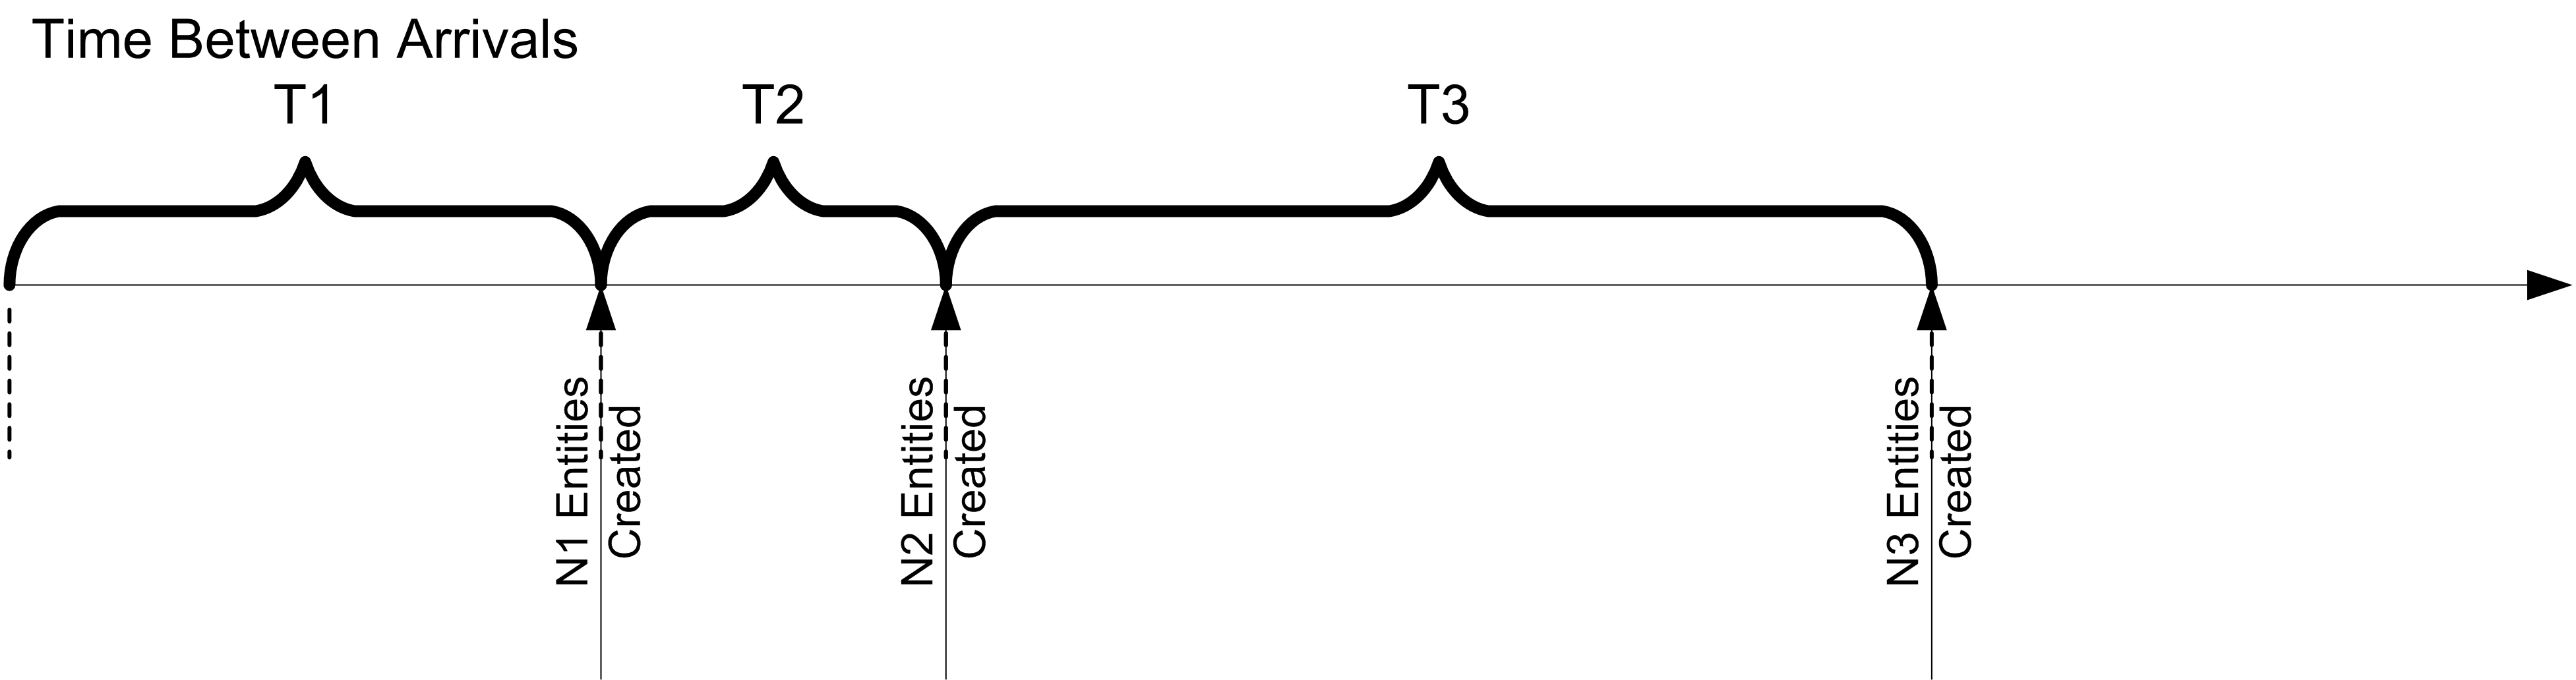
\includegraphics{./figures/ch5/ch5fig3.png}
\caption{\label{fig:ch5EXArrival}Example Arrival Process}
\end{figure}

For example, to specify a Poisson arrival process with mean rate
\(\lambda\), an EventGenerator can be used. Why does this specify a
Poisson arrival process? Because the time between arrivals for a Poisson
process with rate \(\lambda\) is exponentially distributed with the mean
of the exponential distribution being \(1/\lambda\). The the
EventGenerator needs to have its time between arrival distribution
specified as an exponential distribution with mean equal to \(1/\lambda\).
To specify a compound arrival process, use a random variable to
represent the number of occurrences per event. For example, suppose you
have a compound Poisson process\footnote{See \citep{ross1997introduction} for more information on the theory of
  compound Poisson processes.} where the distribution for the
number created at each arrival is governed by a discrete distribution.

\[
P(X = x) =
   \begin{cases}
     0.2 & \quad \text{x = 1}\\
     0.3 & \quad \text{x = 2}\\
     0.5 & \quad \text{x = 3}
   \end{cases}
\]

The following code illustrates how to use an
\texttt{EventGenerator} for this compound Poisson process with the number of
arrivals specified with a discrete empirical random variable. Let's go
through this example before exploring the details of the \texttt{EventGenerator}
class. In line 3 the \texttt{EventGenerator} is declared and in line 17 the
instance of the \texttt{EventGenerator} is created. Notice how the random
variable representing the time between arrivals is provided to
the \texttt{EventGenerator} constructor. The \texttt{EventGenerator} class uses classes
that implement the \texttt{EventGeneratorActionIfc} interface. This interface
defines a single method, called \texttt{generate()}, which is called to supply
logic when the generated event occurs. An inner class
called \texttt{Arrivals} implements the \texttt{EventGeneratorActionIfc} interface.
Notice how a counter is used to count the number of events and a
different counter is used to count the number of arrivals based on the
random variable representing the number of occurrences governed by the
discrete empirical distribution function.

\begin{Shaded}
\begin{Highlighting}[]
\KeywordTok{public} \KeywordTok{class}\NormalTok{ EventGeneratorCPP }\KeywordTok{extends}\NormalTok{ SchedulingElement }\OperatorTok{\{}

    \KeywordTok{protected}\NormalTok{ EventGenerator myArrivalGenerator}\OperatorTok{;}
    \KeywordTok{protected}\NormalTok{ Counter myEventCounter}\OperatorTok{;}
    \KeywordTok{protected}\NormalTok{ Counter myArrivalCounter}\OperatorTok{;}
    \KeywordTok{protected}\NormalTok{ RandomVariable myTBA}\OperatorTok{;}
    \KeywordTok{protected}\NormalTok{ RandomVariable myNumArrivals}\OperatorTok{;}

    \KeywordTok{public} \FunctionTok{EventGeneratorCPP}\OperatorTok{(}\NormalTok{ModelElement parent}\OperatorTok{)} \OperatorTok{\{}
        \KeywordTok{this}\OperatorTok{(}\NormalTok{parent}\OperatorTok{,} \FloatTok{1.0}\OperatorTok{,} \KeywordTok{null}\OperatorTok{);}
    \OperatorTok{\}}

    \KeywordTok{public} \FunctionTok{EventGeneratorCPP}\OperatorTok{(}\NormalTok{ModelElement parent}\OperatorTok{,} \DataTypeTok{double}\NormalTok{ tba}\OperatorTok{,} \BuiltInTok{String}\NormalTok{ name}\OperatorTok{)} \OperatorTok{\{}
        \KeywordTok{super}\OperatorTok{(}\NormalTok{parent}\OperatorTok{,}\NormalTok{ name}\OperatorTok{);}
        \DataTypeTok{double}\OperatorTok{[]}\NormalTok{ values }\OperatorTok{=} \OperatorTok{\{}\DecValTok{1}\OperatorTok{,} \DecValTok{2}\OperatorTok{,} \DecValTok{3}\OperatorTok{\};}
        \DataTypeTok{double}\OperatorTok{[]}\NormalTok{ cdf }\OperatorTok{=} \OperatorTok{\{}\FloatTok{0.2}\OperatorTok{,} \FloatTok{0.5}\OperatorTok{,} \FloatTok{1.0}\OperatorTok{\};}
\NormalTok{        myNumArrivals }\OperatorTok{=} \KeywordTok{new} \FunctionTok{RandomVariable}\OperatorTok{(}\KeywordTok{this}\OperatorTok{,} \KeywordTok{new} \FunctionTok{DEmpiricalRV}\OperatorTok{(}\NormalTok{values}\OperatorTok{,}\NormalTok{ cdf}\OperatorTok{));}
\NormalTok{        myTBA }\OperatorTok{=} \KeywordTok{new} \FunctionTok{RandomVariable}\OperatorTok{(}\KeywordTok{this}\OperatorTok{,} \KeywordTok{new} \FunctionTok{ExponentialRV}\OperatorTok{(}\NormalTok{tba}\OperatorTok{));}
\NormalTok{        myEventCounter }\OperatorTok{=} \KeywordTok{new} \FunctionTok{Counter}\OperatorTok{(}\KeywordTok{this}\OperatorTok{,} \StringTok{"Counts Events"}\OperatorTok{);}
\NormalTok{        myArrivalCounter }\OperatorTok{=} \KeywordTok{new} \FunctionTok{Counter}\OperatorTok{(}\KeywordTok{this}\OperatorTok{,} \StringTok{"Counts Arrivals"}\OperatorTok{);}
\NormalTok{        myArrivalGenerator }\OperatorTok{=} \KeywordTok{new} \FunctionTok{EventGenerator}\OperatorTok{(}\KeywordTok{this}\OperatorTok{,} \KeywordTok{new} \FunctionTok{Arrivals}\OperatorTok{(),}\NormalTok{ myTBA}\OperatorTok{,}\NormalTok{ myTBA}\OperatorTok{);}
    \OperatorTok{\}}

    \KeywordTok{protected} \KeywordTok{class}\NormalTok{ Arrivals }\KeywordTok{implements}\NormalTok{ EventGeneratorActionIfc }\OperatorTok{\{}
        \AttributeTok{@Override}
        \KeywordTok{public} \DataTypeTok{void} \FunctionTok{generate}\OperatorTok{(}\NormalTok{EventGenerator generator}\OperatorTok{,}\NormalTok{ JSLEvent event}\OperatorTok{)} \OperatorTok{\{}
\NormalTok{            myEventCounter}\OperatorTok{.}\FunctionTok{increment}\OperatorTok{();}
            \DataTypeTok{int}\NormalTok{ n }\OperatorTok{=} \OperatorTok{(}\DataTypeTok{int}\OperatorTok{)}\NormalTok{myNumArrivals}\OperatorTok{.}\FunctionTok{getValue}\OperatorTok{();}
\NormalTok{            myArrivalCounter}\OperatorTok{.}\FunctionTok{increment}\OperatorTok{(}\NormalTok{n}\OperatorTok{);}
        \OperatorTok{\}}
    \OperatorTok{\}}
\OperatorTok{\}}
\end{Highlighting}
\end{Shaded}

The \texttt{EventGenerator} class allows for the periodic generation of events
similar to that achieved by ``Create'' modules in other simulation languages.
This class works in conjunction with the \texttt{EventGeneratorActionIfc}
interface, which is used to listen and react to the events that are
generated by this class. Users of the class can supply an instance of an
\texttt{EventGeneratorActionIfc} to provide the actions that take place when
the event occurs. Alternatively, if no \texttt{EventGeneratorActionIfc} is
supplied, by default the \texttt{generator(JSLEvent\ event)} method of this class
will be called when the event occurs. Thus, sub-classes can simply
override this method to provide behavior for when the event occurs. If
no instance of an \texttt{EventGeneratorActionIfc} instance is supplied and the
\texttt{generate()} method is not overridden, then the events will still occur;
however, no meaningful actions will take place. The key input parameters
to the \texttt{EventGenerator} include:

\begin{description}
\item[time until the first event]
This parameter is specified with an object that implements the
\texttt{RandomIfc.} It should be used to represent a positive real value that
represents the time after time 0.0 for the first event to occur. If
this parameter is not supplied, then the first event occurs at time
0.0.
\item[time between events]
This parameter is specified with an object that implements the
\texttt{RandomIfc.} It should be used to represent a positive real value that
represents the time between events. If this parameter is not
supplied, then the time between events is positive infinity.
\item[time until last event]
This parameter is specified with an object that implements the
\texttt{RandomIfc.} It should be used to represent a positive real value that
represents the time that the generator should stop generating. When
the generator is created, this variable is used to set the ending
time of the generator. Each time an event is to be scheduled the
ending time is checked. If the time of the next event is past this
time, then the generator is turned off and the event will not be
scheduled. The default is positive infinity.
\item[maximum number of events]
A value of type long that supplies the maximum number of events to
generate. Each time an event is to be scheduled, the maximum number
of events is checked. If the maximum has been reached, then the
generator is turned off. The default is Long.MAX\_VALUE. This
parameter cannot be Long.MAX\_VALUE when the time until next always
returns a value of 0.0.
\item[listener]
This parameter can be used to supply an instance of
EventGeneratorListenerIfc interface to supply logic to occur when
the event occurs.
\end{description}

The most common use case for an \texttt{EventGenerator} is very similar to the
compound Poisson process example. The \texttt{EventGenerator} is setup to run
with a time between events until the simulation completes; however,
there are a number of other possibilities that are facilitated through
various method associated with the \texttt{EventGenerator} class. The first
possibility is to sub-class the \texttt{EventGenerator} to make a custom
generator for objects of a specific class. To facilitate this the user
need only implement the generate() method that is part of the
\texttt{EventGenerator} class. For example, you could design classes to create
customers, parts, trucks, demands, etc.

In addition to customization through sub-classes, there are a number of
useful methods that are available for controlling the \texttt{EventGenerator.}

\begin{description}
\item[\texttt{turnOffGenerator()}]
This method allows an EventGenerator to be turned off. The next
scheduled generation event will not occur. This method will cancel a
previously scheduled generation event if one exists. No future
events will be scheduled after turning off the generator. Once the
generator has been turned off, it cannot be restarted until the next
replication.
\item[\texttt{turnOnGenerator(GetValueIfc\ t)}]
If the generator was not started upon initialization at the
beginning of a replication, then this method can be used to start
the generator. The generator will be started \(t\) time units after
the call. If this method is used when the generator is already
started it does nothing. If this method is used after the generator
is done it does nothing. If this method is used after the generator
has been suspended it does nothing. In other words, if the generator
is already on, this method does nothing.
\item[\texttt{suspend()}]
This method suspends the event generation pattern. The generator is
still on, but the generation of events is suspended. The next
scheduled generation event is canceled.
\item[\texttt{resume()}]
If the generator is suspended then this method causes the event
generator to proceed with the event generation pattern by scheduling
a new event according to the time between event distribution.
\item[\texttt{isSuspended()}]
Checks if the generator is suspended.
\item[\texttt{isGeneratorDone()}]
Checks if the generator has been turned off. The generator can be
turned off via the turnOffGenerator() method or it may turn off when
it has reached its time until last event or if the maximum number of
events is reached. As previously noted, once a generator has been
turned off, it cannot be turned on again within the same
replication.
\end{description}

In considering these methods, a generator can turn itself off (as an
action) within or caused by the code within its generate() method or in
the supplied \texttt{EventGeneratorListenerIfc} interface. It might also
\texttt{suspend()} itself in a similar manner. Of course, a class that has a
reference to the generator may also turn it off or suspend it. To resume
a suspended event generator, it is necessary to schedule an event whose
action invokes the \texttt{resume()}method. Obviously, this can be within a
sub-class of \texttt{EventGenerator} or within another class that has a reference
to the event generator.

\hypertarget{dem:station}{%
\section{The Station Package}\label{dem:station}}

This section describes a JSL package that facilitates the modeling of
system components that can send or receive entities. Many systems have
as a basic component a location where something happens or where
processing can occur. A station represents this concept. The goal of
this package is to illustrate the development and use of common
components that help with the modeling of simple queueing system
modeling. First, an overview of the package will be presented and then
the operation of important classes discussed. Then, a number of examples
will illustrate how to utilize the classes.

\begin{figure}
\centering
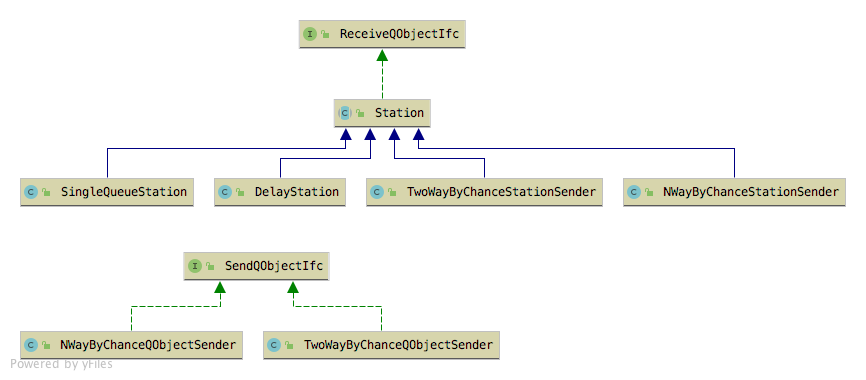
\includegraphics{./figures/ch5/StationPkg.png}
\caption{\label{fig:StationPkg}Major Classes within Station Package}
\end{figure}

Figure \ref{fig:StationPkg} illustrates the primary classes and
interfaces within the station package. There are two key interfaces:
\texttt{SendQObjectIfc} and \texttt{ReceiveQObjectIfc}.

\begin{Shaded}
\begin{Highlighting}[]
\KeywordTok{public} \KeywordTok{interface}\NormalTok{ SendQObjectIfc }\OperatorTok{\{}
    
    \DataTypeTok{void} \FunctionTok{send}\OperatorTok{(}\NormalTok{QObject qObj}\OperatorTok{);}
\OperatorTok{\}}

\KeywordTok{public} \KeywordTok{interface}\NormalTok{ ReceiveQObjectIfc }\OperatorTok{\{}

    \DataTypeTok{void} \FunctionTok{receive}\OperatorTok{(}\NormalTok{QObject qObj}\OperatorTok{);}
\OperatorTok{\}}
\end{Highlighting}
\end{Shaded}

The interfaces define single methods, \texttt{send(QObject\ qObj)} and \texttt{receive(QObject\ qObj)}, which permit
implementors to promise the capability of receiving and sending objects
of type \texttt{QObject}. Figure \ref{fig:Station} illustrates the connection between the Station class and \texttt{SendQObjectIfc} and \texttt{ReceiveQObjectIfc}. This design permits the development of model elements that
know how to send instances of \texttt{QObject} and how to receive instances of
\texttt{QObject}. A \texttt{Station} is an abstract base class that implements the
\texttt{ReceiveQObjectIfc} interface. Sub-classes of \texttt{Station} will have a
\texttt{receive()} method that can be called to tell the station that an instance
of a \texttt{QObject} should be received.

\begin{figure}
\centering
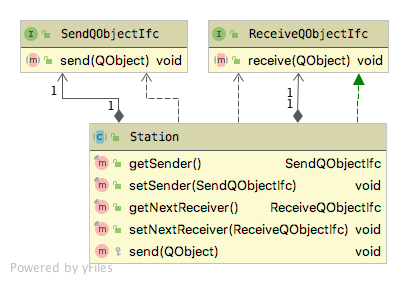
\includegraphics{./figures/ch5/Station.png}
\caption{\label{fig:Station}The Station Class}
\end{figure}

The following listing shows the implementation of the \texttt{Station}
class. The \texttt{Station} class may have a reference to an object that
implements the \texttt{SendQObjectIfc} interface and may have an object that implements
the \texttt{ReceiveQObjectIfc} interface. An object that implements the
\texttt{SendQObjectIfc} interface can be supplied to define behavior for sending
a received instance of a \texttt{QObject} onwards within the system. If the
\texttt{SendQObjectIfc} interface attribute is not supplied, then the
\texttt{ReceiveQObjectIfc} object is used to indicate the next location for
receipt. The protected method, s\texttt{end(QObject\ qObj)},
indicates this logic. The UML diagram for the \texttt{Station} class is provided
in Figure \ref{fig:Station}. Notice that \texttt{Station} implements the
\texttt{ReceiveQObjectIfc} interface, may have a reference to a \texttt{ReceiveQObjectIfc}
instance, and has a reference to an instance of a \texttt{SendQObjectIfc}
interface.

If the client does not supplier either an object that implements the \texttt{ReceiveQObjectIfc} interface or an object that implements the \texttt{SendQObjectIfc} interface, then an exception will be thrown. The object that implements the \texttt{ReceiveQObjectIfc} interface is meant to be a direct connection (i.e.~something that can directly receive instances of \texttt{QObject}). Sometimes, the logic to determine where to send the \texttt{QObject} is complex. In which case, the user can either sub-class the \texttt{Station} class or provide a instance of a class that implements the \texttt{SendQObjectIfc} interface. This allows the sending logic to be delegated to another class rather than forcing the user to sub-class the \texttt{Station} class. This flexibility can be confusing to users of the class.

\begin{Shaded}
\begin{Highlighting}[]
\KeywordTok{public} \KeywordTok{abstract} \KeywordTok{class}\NormalTok{ Station }\KeywordTok{extends}\NormalTok{ SchedulingElement }\KeywordTok{implements}\NormalTok{ ReceiveQObjectIfc }\OperatorTok{\{}

    \CommentTok{/**}
     \CommentTok{*}\NormalTok{ Can be supplied in order to provide logic}
     \CommentTok{*}\NormalTok{  to send the QObject to its next receiver}
     \CommentTok{*/}
    \KeywordTok{private}\NormalTok{ SendQObjectIfc mySender}\OperatorTok{;}

    \CommentTok{/**}\NormalTok{ Can be used to directly tell the receiver to receive the departing}
     \CommentTok{*}\NormalTok{  QObject}
     \CommentTok{*} 
     \CommentTok{*/}
    \KeywordTok{private}\NormalTok{ ReceiveQObjectIfc myNextReceiver}\OperatorTok{;}

    \CommentTok{/**}
     \CommentTok{*}
\CommentTok{     * @}\NormalTok{param parent the parent model element}
     \CommentTok{*/}
    \KeywordTok{public} \FunctionTok{Station}\OperatorTok{(}\NormalTok{ModelElement parent}\OperatorTok{)} \OperatorTok{\{}
        \KeywordTok{this}\OperatorTok{(}\NormalTok{parent}\OperatorTok{,} \KeywordTok{null}\OperatorTok{,} \KeywordTok{null}\OperatorTok{);}
    \OperatorTok{\}}

    \CommentTok{/**}
     \CommentTok{*}
\CommentTok{     * @}\NormalTok{param parent the parent model element}
     \CommentTok{*} \CommentTok{@}\NormalTok{param name a unique name}
     \CommentTok{*/}
    \KeywordTok{public} \FunctionTok{Station}\OperatorTok{(}\NormalTok{ModelElement parent}\OperatorTok{,} \BuiltInTok{String}\NormalTok{ name}\OperatorTok{)} \OperatorTok{\{}
        \KeywordTok{this}\OperatorTok{(}\NormalTok{parent}\OperatorTok{,} \KeywordTok{null}\OperatorTok{,}\NormalTok{ name}\OperatorTok{);}
    \OperatorTok{\}}

    \CommentTok{/**}
     \CommentTok{*} 
\CommentTok{     * @}\NormalTok{param parent the parent model element}
     \CommentTok{*} \CommentTok{@}\NormalTok{param sender can be null}\CommentTok{,}\NormalTok{ represents something that can send QObjects}
     \CommentTok{*} \CommentTok{@}\NormalTok{param name a unique name}
     \CommentTok{*/}
    \KeywordTok{public} \FunctionTok{Station}\OperatorTok{(}\NormalTok{ModelElement parent}\OperatorTok{,}\NormalTok{ SendQObjectIfc sender}\OperatorTok{,} \BuiltInTok{String}\NormalTok{ name}\OperatorTok{)} \OperatorTok{\{}
        \KeywordTok{super}\OperatorTok{(}\NormalTok{parent}\OperatorTok{,}\NormalTok{ name}\OperatorTok{);}
        \FunctionTok{setSender}\OperatorTok{(}\NormalTok{sender}\OperatorTok{);}
    \OperatorTok{\}}

    \CommentTok{/**}
     \CommentTok{*}\NormalTok{ A Station may or may not have a helper object that implements the }
     \CommentTok{*}\NormalTok{  SendQObjectIfc interface}\CommentTok{. }\NormalTok{ If this helper object is supplied it will}
     \CommentTok{*}\NormalTok{  be used to send the processed QObject to its next location for}
     \CommentTok{*}\NormalTok{  processing}\CommentTok{.}
     \CommentTok{*} \CommentTok{@}\NormalTok{return the thing that will be used to send the completed QObject}
     \CommentTok{*/}
    \KeywordTok{public} \DataTypeTok{final}\NormalTok{ SendQObjectIfc }\FunctionTok{getSender}\OperatorTok{()} \OperatorTok{\{}
        \ControlFlowTok{return}\NormalTok{ mySender}\OperatorTok{;}
    \OperatorTok{\}}

    \CommentTok{/**}
     \CommentTok{*}\NormalTok{ A Station may or may not have a helper object that implements the }
     \CommentTok{*}\NormalTok{  SendQObjectIfc interface}\CommentTok{. }\NormalTok{ If this helper object is supplied it will}
     \CommentTok{*}\NormalTok{  be used to send the processed QObject to its next location for}
     \CommentTok{*}\NormalTok{  processing}\CommentTok{.}
     \CommentTok{*} \CommentTok{@}\NormalTok{param sender the thing that will be used to send the completed QObject}
     \CommentTok{*/}
    \KeywordTok{public} \DataTypeTok{final} \DataTypeTok{void} \FunctionTok{setSender}\OperatorTok{(}\NormalTok{SendQObjectIfc sender}\OperatorTok{)} \OperatorTok{\{}
\NormalTok{        mySender }\OperatorTok{=}\NormalTok{ sender}\OperatorTok{;}
    \OperatorTok{\}}

    \CommentTok{/**}
     \CommentTok{*}\NormalTok{  A Station may or may not have a helper object that implements the }
     \CommentTok{*}\NormalTok{  ReceiveQObjectIfc interface}\CommentTok{. }\NormalTok{ If this helper object is supplied and}
     \CommentTok{*}\NormalTok{  the SendQObjectIfc helper is not supplied}\CommentTok{,}\NormalTok{ then the object that implements}
     \CommentTok{*}\NormalTok{  the ReceiveQObjectIfc will be the next receiver for the QObject when using }
     \CommentTok{*}\NormalTok{  default send}\CommentTok{()}\NormalTok{ method}\CommentTok{.}
     \CommentTok{*} \CommentTok{@}\NormalTok{return the thing that should receive the completed QObject}\CommentTok{,}\NormalTok{ may be null}
     \CommentTok{*/}
    \KeywordTok{public} \DataTypeTok{final}\NormalTok{ ReceiveQObjectIfc }\FunctionTok{getNextReceiver}\OperatorTok{()} \OperatorTok{\{}
        \ControlFlowTok{return}\NormalTok{ myNextReceiver}\OperatorTok{;}
    \OperatorTok{\}}

    \CommentTok{/**}
     \CommentTok{*}\NormalTok{  A Station may or may not have a helper object that implements the }
     \CommentTok{*}\NormalTok{  ReceiveQObjectIfc interface}\CommentTok{. }\NormalTok{ If this helper object is supplied and}
     \CommentTok{*}\NormalTok{  the SendQObjectIfc helper is not supplied}\CommentTok{,}\NormalTok{ then the object that implements}
     \CommentTok{*}\NormalTok{  the ReceiveQObjectIfc will be the next receiver for the QObject when using }
     \CommentTok{*}\NormalTok{  default send}\CommentTok{()}\NormalTok{ method}\CommentTok{.}
     \CommentTok{*} \CommentTok{@}\NormalTok{param receiver the thing that should receive the completed QObject}\CommentTok{,}\NormalTok{ may be null}
     \CommentTok{*/}
    \KeywordTok{public} \DataTypeTok{final} \DataTypeTok{void} \FunctionTok{setNextReceiver}\OperatorTok{(}\NormalTok{ReceiveQObjectIfc receiver}\OperatorTok{)} \OperatorTok{\{}
\NormalTok{        myNextReceiver }\OperatorTok{=}\NormalTok{ receiver}\OperatorTok{;}
    \OperatorTok{\}}

    \CommentTok{/**}
     \CommentTok{*}\NormalTok{  A Station may or may not have a helper object that implements the }
     \CommentTok{*}\NormalTok{  SendQObjectIfc interface}\CommentTok{. }\NormalTok{ If this helper object is supplied it will}
     \CommentTok{*}\NormalTok{  be used to send the processed QObject to its next location for}
     \CommentTok{*}\NormalTok{  processing}\CommentTok{.}
     \CommentTok{*} 
     \CommentTok{*}\NormalTok{  A Station may or may not have a helper object that implements the }
     \CommentTok{*}\NormalTok{  ReceiveQObjectIfc interface}\CommentTok{.}\NormalTok{  If this helper object is supplied and}
     \CommentTok{*}\NormalTok{  the SendQObjectIfc helper is not supplied}\CommentTok{,}\NormalTok{ then the object that implements}
     \CommentTok{*}\NormalTok{  the ReceiveQObjectIfc will be the next receiver for the QObject}
     \CommentTok{*} 
     \CommentTok{*}\NormalTok{  If neither helper object is supplied then a runtime exception will}
     \CommentTok{*}\NormalTok{  occur when trying to use the send}\CommentTok{()}\NormalTok{ method     }
     \CommentTok{*} \CommentTok{@}\NormalTok{param qObj the completed QObject}
     \CommentTok{*/}
    \KeywordTok{protected} \DataTypeTok{void} \FunctionTok{send}\OperatorTok{(}\NormalTok{QObject qObj}\OperatorTok{)} \OperatorTok{\{}
        \ControlFlowTok{if} \OperatorTok{(}\FunctionTok{getSender}\OperatorTok{()} \OperatorTok{!=} \KeywordTok{null}\OperatorTok{)} \OperatorTok{\{}
            \FunctionTok{getSender}\OperatorTok{().}\FunctionTok{send}\OperatorTok{(}\NormalTok{qObj}\OperatorTok{);}
        \OperatorTok{\}} \ControlFlowTok{else} \ControlFlowTok{if} \OperatorTok{(}\FunctionTok{getNextReceiver}\OperatorTok{()} \OperatorTok{!=} \KeywordTok{null}\OperatorTok{)} \OperatorTok{\{}
            \FunctionTok{getNextReceiver}\OperatorTok{().}\FunctionTok{receive}\OperatorTok{(}\NormalTok{qObj}\OperatorTok{);}
        \OperatorTok{\}} \ControlFlowTok{else} \OperatorTok{\{}
            \ControlFlowTok{throw} \KeywordTok{new} \BuiltInTok{RuntimeException}\OperatorTok{(}\StringTok{"No valid sender or receiver"}\OperatorTok{);}
        \OperatorTok{\}}
    \OperatorTok{\}}

\OperatorTok{\}}
\end{Highlighting}
\end{Shaded}

\hypertarget{modeling-simple-queueing-stations}{%
\subsection{Modeling Simple Queueing Stations}\label{modeling-simple-queueing-stations}}

In this section, the station package is used to implement a simple
queueing station. Recall the pharmacy model. In that model, we had a Poisson arrival
process with customers arriving to a drive through pharmacy window. The
service time associated with the pharmacy was exponentially distributed
and their was one pharmacist. That situation was labeled as a M/M/1
queue. In this example, we generalize the queueing station to a G/G/c
queue. That is, any general (G) arrival process, any general (G) service
process, and (c) servers. We will model the arrival process using an
\texttt{EventGenerator} and model the queueing with a \texttt{Queue} class. In addition,
we will generalize the concept of the servers by encapsulating them in a
class called \texttt{SResource} (for simple resource). Finally, the \texttt{Queue} and the
\texttt{SResource} classes will be combined into one class that sub-classes
\texttt{Station}, called \texttt{SingleQueueStation}. This is illustrated in
Figure \ref{fig:GGCQueuingStation}.

\begin{figure}
\centering
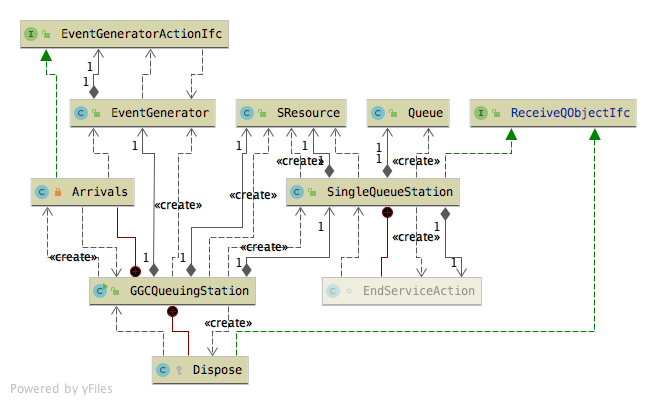
\includegraphics{./figures/ch5/GGCQueuingStation.png}
\caption{\label{fig:GGCQueuingStation}GGC Queueing Station Classes}
\end{figure}

In the figure, the \texttt{GGCQueueingStation} class uses inner classes for
handling the arrivals and for disposing customers that have completed
service. In addition, \texttt{GGCQueueingStation} uses an instance of
\texttt{SingleQueueStation} to process the customers after arrival.

Let's first examine the organization of the \texttt{GGCQueueingStation} class and
how it works with the \texttt{Station} package. Then, we will present how the
\texttt{SingleQueueStation} class was implemented. As shown in
Figure \ref{fig:GGCQueuingStation}
the \texttt{GGCQueueingStation} class uses an instance of \texttt{EventGenerator.} The
event generator's action is called \texttt{Arrivals}, which is implemented as
an inner class of \texttt{GGCQueueingStation.} Secondly, \texttt{GGCQueueingStation} uses
an instance of the class \texttt{Dispose}, which implements the \texttt{ReceiveQObjectIfc}
interface. This instance is used as the receiver after processing by the
\texttt{SingleQueueStation} class. The class collects some system level
statistics.

The following code listing shows the code for the GGCQueueingStation
class. The constructor takes in instances of RandomIfc interfaces to
represent the arrival and service processes. The arrival generator and
statistical collection model elements are created within the constructor.
The third line of the constructor creates the resource that is used by the arriving customers.
The fifth line of the constructor creates an instance of a \texttt{SingleQueueStation} to handle the
customers. Notice that the next line defines the next receiver for the station
to be an instance of the class \texttt{Dispose}. When the \texttt{SingleQueueStation} is
done, the \texttt{send()} method is called (as previously described) and since a
receiver has been attached, the station uses this receiver to receive
the \texttt{QObject} that was completed. In this case, the \texttt{QObject} has statistics
collected as it leaves the system. The only other code
to note is how the EventGenerator's action is used to send the \texttt{QObject}
to the \texttt{SingleQueueStation}. Within the \texttt{Arrivals} class, the \texttt{receive()} method of the \texttt{SingleQueueStation} instance is called with the created \texttt{QObject}. In essence, the
\texttt{GGCQueueingStation} class simply defines and hooks up the various
components needed to model the situation. The \texttt{RecieveQObjectIfc} and the
\texttt{Station} concept play an integral role in facilitating how the object
instances are connected.

\begin{Shaded}
\begin{Highlighting}[]
\KeywordTok{public} \KeywordTok{class}\NormalTok{ GGCQueuingStation }\KeywordTok{extends}\NormalTok{ ModelElement }\OperatorTok{\{}

    \KeywordTok{private} \DataTypeTok{final}\NormalTok{ EventGenerator myArrivalGenerator}\OperatorTok{;}
    \KeywordTok{private} \DataTypeTok{final}\NormalTok{ SingleQueueStation mySQS}\OperatorTok{;}
    \KeywordTok{private}\NormalTok{ ResponseVariable mySystemTime}\OperatorTok{;}
    \KeywordTok{private}\NormalTok{ TimeWeighted myNumInSystem}\OperatorTok{;}
    \KeywordTok{private} \DataTypeTok{final}\NormalTok{ SResource myServers}\OperatorTok{;}
    \KeywordTok{private} \DataTypeTok{final}\NormalTok{ RandomVariable mySTRV}\OperatorTok{;}

    \KeywordTok{public} \FunctionTok{GGCQueuingStation}\OperatorTok{(}\NormalTok{ModelElement parent}\OperatorTok{,}\NormalTok{ RandomIfc tba}\OperatorTok{,}\NormalTok{ RandomIfc st}\OperatorTok{,}
            \DataTypeTok{int}\NormalTok{ numServers}\OperatorTok{)} \OperatorTok{\{}
        \KeywordTok{this}\OperatorTok{(}\NormalTok{parent}\OperatorTok{,}\NormalTok{ tba}\OperatorTok{,}\NormalTok{ st}\OperatorTok{,}\NormalTok{ numServers}\OperatorTok{,} \KeywordTok{null}\OperatorTok{);}
    \OperatorTok{\}}

    \KeywordTok{public} \FunctionTok{GGCQueuingStation}\OperatorTok{(}\NormalTok{ModelElement parent}\OperatorTok{,}\NormalTok{ RandomIfc tba}\OperatorTok{,}\NormalTok{ RandomIfc st}\OperatorTok{,}
                             \DataTypeTok{int}\NormalTok{ numServers}\OperatorTok{,} \BuiltInTok{String}\NormalTok{ name}\OperatorTok{)} \OperatorTok{\{}
        \KeywordTok{super}\OperatorTok{(}\NormalTok{parent}\OperatorTok{,}\NormalTok{ name}\OperatorTok{);}
\NormalTok{        myArrivalGenerator }\OperatorTok{=} \KeywordTok{new} \FunctionTok{EventGenerator}\OperatorTok{(}\KeywordTok{this}\OperatorTok{,} \KeywordTok{new} \FunctionTok{Arrivals}\OperatorTok{(),}\NormalTok{ tba}\OperatorTok{,}\NormalTok{ tba}\OperatorTok{);}
\NormalTok{        myServers }\OperatorTok{=} \KeywordTok{new} \FunctionTok{SResource}\OperatorTok{(}\KeywordTok{this}\OperatorTok{,}\NormalTok{ numServers}\OperatorTok{,} \StringTok{"Servers"}\OperatorTok{);}
\NormalTok{        mySTRV }\OperatorTok{=} \KeywordTok{new} \FunctionTok{RandomVariable}\OperatorTok{(}\KeywordTok{this}\OperatorTok{,}\NormalTok{ st}\OperatorTok{);}
\NormalTok{        mySQS }\OperatorTok{=} \KeywordTok{new} \FunctionTok{SingleQueueStation}\OperatorTok{(}\KeywordTok{this}\OperatorTok{,}\NormalTok{ myServers}\OperatorTok{,}\NormalTok{ mySTRV}\OperatorTok{,} \StringTok{"Station"}\OperatorTok{);}
\NormalTok{        mySQS}\OperatorTok{.}\FunctionTok{setNextReceiver}\OperatorTok{(}\KeywordTok{new} \FunctionTok{Dispose}\OperatorTok{());}
\NormalTok{        mySystemTime }\OperatorTok{=} \KeywordTok{new} \FunctionTok{ResponseVariable}\OperatorTok{(}\KeywordTok{this}\OperatorTok{,} \StringTok{"System Time"}\OperatorTok{);}
\NormalTok{        myNumInSystem }\OperatorTok{=} \KeywordTok{new} \FunctionTok{TimeWeighted}\OperatorTok{(}\KeywordTok{this}\OperatorTok{,} \StringTok{"Num in System"}\OperatorTok{);}
    \OperatorTok{\}}

    \KeywordTok{private} \KeywordTok{class}\NormalTok{ Arrivals }\KeywordTok{implements}\NormalTok{ EventGeneratorActionIfc }\OperatorTok{\{}

        \AttributeTok{@Override}
        \KeywordTok{public} \DataTypeTok{void} \FunctionTok{generate}\OperatorTok{(}\NormalTok{EventGenerator generator}\OperatorTok{,}\NormalTok{ JSLEvent event}\OperatorTok{)} \OperatorTok{\{}
\NormalTok{            myNumInSystem}\OperatorTok{.}\FunctionTok{increment}\OperatorTok{();}
\NormalTok{            mySQS}\OperatorTok{.}\FunctionTok{receive}\OperatorTok{(}\KeywordTok{new} \FunctionTok{QObject}\OperatorTok{(}\FunctionTok{getTime}\OperatorTok{()));}
        \OperatorTok{\}}

    \OperatorTok{\}}

    \KeywordTok{protected} \KeywordTok{class}\NormalTok{ Dispose }\KeywordTok{implements}\NormalTok{ ReceiveQObjectIfc }\OperatorTok{\{}

        \AttributeTok{@Override}
        \KeywordTok{public} \DataTypeTok{void} \FunctionTok{receive}\OperatorTok{(}\NormalTok{QObject qObj}\OperatorTok{)} \OperatorTok{\{}
            \CommentTok{// collect final statistics}
\NormalTok{            myNumInSystem}\OperatorTok{.}\FunctionTok{decrement}\OperatorTok{();}
\NormalTok{            mySystemTime}\OperatorTok{.}\FunctionTok{setValue}\OperatorTok{(}\FunctionTok{getTime}\OperatorTok{()} \OperatorTok{{-}}\NormalTok{ qObj}\OperatorTok{.}\FunctionTok{getCreateTime}\OperatorTok{());}
        \OperatorTok{\}}

    \OperatorTok{\}}
\end{Highlighting}
\end{Shaded}

The last piece of this puzzle is how the \texttt{SingleQueueStation} class
implements the abstract base class \texttt{Station} and becomes a component that
can be reused in various models. Recall the logic for handling arrivals
and service completions from the pharmacy example. In that code, there was the need to have
the customer enter the queue and then check if the pharmacist was
available. If the pharmacist was available, then the customer was
removed from the queue and the end of service scheduled. In addition,
when the service is completed, if the queue is not empty, then the next
customer is started into service. The \texttt{SingleQueueStation} generalizes this
same logic by using an instance of \texttt{SResource} to represent the servers.

The following code listing illustrates the critical code for the
\texttt{SingleQueueStation} class. The \texttt{receive()} method (which must be
implemented by a sub-class of \texttt{Station}), shows the \texttt{QObject} being placed
in the queue. Then, the resource is checked to
see if it is available and then the next customer is served via the call
to \texttt{serveNext()}. Upon the end of service the \texttt{EndServiceAction} is called.
Notice that the resource is released, and then the queue is
checked. Finally, the \texttt{send()} method is used to send the
\texttt{QObject} to whereever it is intended to go.

\begin{Shaded}
\begin{Highlighting}[]
    \KeywordTok{protected} \DataTypeTok{double} \FunctionTok{getServiceTime}\OperatorTok{(}\NormalTok{QObject customer}\OperatorTok{)} \OperatorTok{\{}
        \DataTypeTok{double}\NormalTok{ t}\OperatorTok{;}
        \ControlFlowTok{if} \OperatorTok{(}\FunctionTok{getUseQObjectServiceTimeOption}\OperatorTok{())} \OperatorTok{\{}
\NormalTok{            Optional}\OperatorTok{\textless{}}\NormalTok{GetValueIfc}\OperatorTok{\textgreater{}}\NormalTok{ valueObject }\OperatorTok{=}\NormalTok{ customer}\OperatorTok{.}\FunctionTok{getValueObject}\OperatorTok{();}
            \ControlFlowTok{if} \OperatorTok{(}\NormalTok{valueObject}\OperatorTok{.}\FunctionTok{isPresent}\OperatorTok{())\{}
\NormalTok{                t }\OperatorTok{=}\NormalTok{ valueObject}\OperatorTok{.}\FunctionTok{get}\OperatorTok{().}\FunctionTok{getValue}\OperatorTok{();}
            \OperatorTok{\}} \ControlFlowTok{else} \OperatorTok{\{}
                \ControlFlowTok{throw} \KeywordTok{new} \BuiltInTok{IllegalStateException}\OperatorTok{(}\StringTok{"Attempted to use QObject.getValueObject() when no object was set"}\OperatorTok{);}
            \OperatorTok{\}}
        \OperatorTok{\}} \ControlFlowTok{else} \OperatorTok{\{}
\NormalTok{            t }\OperatorTok{=} \FunctionTok{getServiceTime}\OperatorTok{().}\FunctionTok{getValue}\OperatorTok{();}
        \OperatorTok{\}}
        \ControlFlowTok{return}\NormalTok{ t}\OperatorTok{;}
    \OperatorTok{\}}

    \CommentTok{/**}
     \CommentTok{*}\NormalTok{ Called to determine which waiting QObject will be served next Determines}
     \CommentTok{*}\NormalTok{ the next customer}\CommentTok{,}\NormalTok{ seizes the resource}\CommentTok{,}\NormalTok{ and schedules the end of the}
     \CommentTok{*}\NormalTok{ service}\CommentTok{.}
     \CommentTok{*/}
    \KeywordTok{protected} \DataTypeTok{void} \FunctionTok{serveNext}\OperatorTok{()} \OperatorTok{\{}
\NormalTok{        QObject customer }\OperatorTok{=}\NormalTok{ myWaitingQ}\OperatorTok{.}\FunctionTok{removeNext}\OperatorTok{();} \CommentTok{//remove the next customer}
\NormalTok{        myResource}\OperatorTok{.}\FunctionTok{seize}\OperatorTok{();}
        \CommentTok{// schedule end of service}
        \FunctionTok{scheduleEvent}\OperatorTok{(}\NormalTok{myEndServiceAction}\OperatorTok{,} \FunctionTok{getServiceTime}\OperatorTok{(}\NormalTok{customer}\OperatorTok{),}\NormalTok{ customer}\OperatorTok{);}
    \OperatorTok{\}}

    \AttributeTok{@Override}
    \KeywordTok{public} \DataTypeTok{void} \FunctionTok{receive}\OperatorTok{(}\NormalTok{QObject customer}\OperatorTok{)} \OperatorTok{\{}
\NormalTok{        myNS}\OperatorTok{.}\FunctionTok{increment}\OperatorTok{();} \CommentTok{// new customer arrived}
\NormalTok{        myWaitingQ}\OperatorTok{.}\FunctionTok{enqueue}\OperatorTok{(}\NormalTok{customer}\OperatorTok{);} \CommentTok{// enqueue the newly arriving customer}
        \ControlFlowTok{if} \OperatorTok{(}\FunctionTok{isResourceAvailable}\OperatorTok{())} \OperatorTok{\{} \CommentTok{// server available}
            \FunctionTok{serveNext}\OperatorTok{();}
        \OperatorTok{\}}
    \OperatorTok{\}}

    \KeywordTok{class}\NormalTok{ EndServiceAction }\KeywordTok{implements}\NormalTok{ EventActionIfc}\OperatorTok{\textless{}}\NormalTok{QObject}\OperatorTok{\textgreater{}} \OperatorTok{\{}

        \AttributeTok{@Override}
        \KeywordTok{public} \DataTypeTok{void} \FunctionTok{action}\OperatorTok{(}\NormalTok{JSLEvent}\OperatorTok{\textless{}}\NormalTok{QObject}\OperatorTok{\textgreater{}}\NormalTok{ event}\OperatorTok{)} \OperatorTok{\{}
\NormalTok{            QObject leavingCustomer }\OperatorTok{=}\NormalTok{ event}\OperatorTok{.}\FunctionTok{getMessage}\OperatorTok{();}
\NormalTok{            myNS}\OperatorTok{.}\FunctionTok{decrement}\OperatorTok{();} \CommentTok{// customer departed}
\NormalTok{            myResource}\OperatorTok{.}\FunctionTok{release}\OperatorTok{();}
            \ControlFlowTok{if} \OperatorTok{(}\FunctionTok{isQueueNotEmpty}\OperatorTok{())} \OperatorTok{\{} \CommentTok{// queue is not empty}
                \FunctionTok{serveNext}\OperatorTok{();}
            \OperatorTok{\}}
            \FunctionTok{send}\OperatorTok{(}\NormalTok{leavingCustomer}\OperatorTok{);}
        \OperatorTok{\}}
    \OperatorTok{\}}
\end{Highlighting}
\end{Shaded}

This is the same \texttt{send()} method that was previously discussed. Thus, because the receiver was set to be
the instance of \texttt{Dispose}, the departing customer will be sent to the
\texttt{GGCQueueingStation} where the statistics will be collected, as previously
noted.

Figure \ref{fig:SResource} shows the \texttt{SResource} class. The \texttt{SResource}
class models a resource that has a defined capacity, which represents
the number of units of the resource that can be in use. The capacity of
the resource represents the maximum number of units available for use.
For example, if the resource has capacity 3, it may have 2 units busy
and 1 unit idle. A resource cannot have more units busy than the
capacity. A resource is considered busy when it has 1 or more units
busy. A resource is considered idle when all available units are idle.
Units of the resource can be seized via the \texttt{seize()} methods and released
via the \texttt{release()} methods. It is an error to attempt to seize more units
than are currently available. In addition, it is an error to try to
\texttt{release()} more units than are currently in use (busy). Statistics on
resource utilization and number of busy units is automatically
collected.

\begin{figure}
\centering
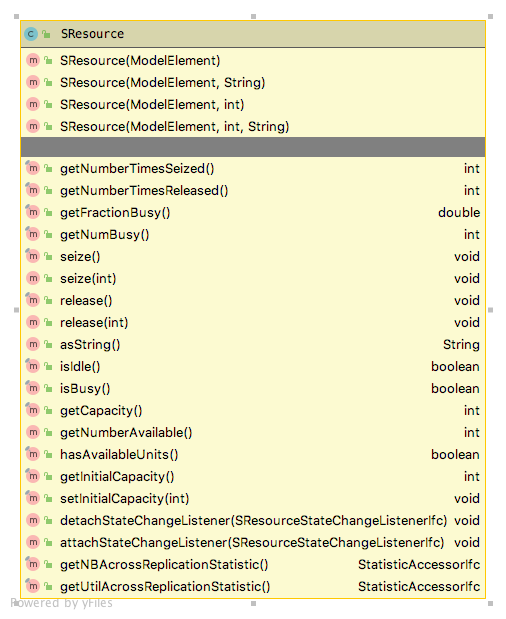
\includegraphics{./figures/ch5/SResource.png}
\caption{\label{fig:SResource}The SResource Class}
\end{figure}

The following listing illustrates how to build and run an
instance of a GGCQueuingStation by simulating a M/M/2 queue.

\begin{Shaded}
\begin{Highlighting}[]
    \KeywordTok{public} \DataTypeTok{static} \DataTypeTok{void} \FunctionTok{main}\OperatorTok{(}\BuiltInTok{String}\OperatorTok{[]}\NormalTok{ args}\OperatorTok{)} \OperatorTok{\{}
\NormalTok{        Simulation sim }\OperatorTok{=} \KeywordTok{new} \FunctionTok{Simulation}\OperatorTok{(}\StringTok{"M/M/2"}\OperatorTok{);}
        \CommentTok{// get the model}
\NormalTok{        Model m }\OperatorTok{=}\NormalTok{ sim}\OperatorTok{.}\FunctionTok{getModel}\OperatorTok{();}
        \CommentTok{// add system to the main model}
\NormalTok{        ExponentialRV tba }\OperatorTok{=} \KeywordTok{new} \FunctionTok{ExponentialRV}\OperatorTok{(}\DecValTok{1}\OperatorTok{);}
\NormalTok{        ExponentialRV st }\OperatorTok{=} \KeywordTok{new} \FunctionTok{ExponentialRV}\OperatorTok{(}\FloatTok{.8}\OperatorTok{);}
        \DataTypeTok{int}\NormalTok{ ns }\OperatorTok{=} \DecValTok{2}\OperatorTok{;}
\NormalTok{        GGCQueuingStation system }\OperatorTok{=} \KeywordTok{new} \FunctionTok{GGCQueuingStation}\OperatorTok{(}\NormalTok{m}\OperatorTok{,}\NormalTok{ tba}\OperatorTok{,}\NormalTok{ st}\OperatorTok{,}\NormalTok{ ns}\OperatorTok{);}
        \CommentTok{// set the parameters of the experiment}
\NormalTok{        sim}\OperatorTok{.}\FunctionTok{setNumberOfReplications}\OperatorTok{(}\DecValTok{30}\OperatorTok{);}
\NormalTok{        sim}\OperatorTok{.}\FunctionTok{setLengthOfReplication}\OperatorTok{(}\FloatTok{20000.0}\OperatorTok{);}
\NormalTok{        sim}\OperatorTok{.}\FunctionTok{setLengthOfWarmUp}\OperatorTok{(}\FloatTok{5000.0}\OperatorTok{);}
\NormalTok{        SimulationReporter r }\OperatorTok{=}\NormalTok{ sim}\OperatorTok{.}\FunctionTok{makeSimulationReporter}\OperatorTok{();}
        \BuiltInTok{System}\OperatorTok{.}\FunctionTok{out}\OperatorTok{.}\FunctionTok{println}\OperatorTok{(}\StringTok{"Simulation started."}\OperatorTok{);}
\NormalTok{        sim}\OperatorTok{.}\FunctionTok{run}\OperatorTok{();}
        \BuiltInTok{System}\OperatorTok{.}\FunctionTok{out}\OperatorTok{.}\FunctionTok{println}\OperatorTok{(}\StringTok{"Simulation completed."}\OperatorTok{);}
\NormalTok{        r}\OperatorTok{.}\FunctionTok{printAcrossReplicationSummaryStatistics}\OperatorTok{();}
    \OperatorTok{\}}
\end{Highlighting}
\end{Shaded}

This is the same as any JSL run. In this case, the \texttt{GGCQueueingStation} class used a
\texttt{SingleQueueStation} to do, essentially, all of the work. Now, imagine
many queueing stations organized into a system. Because the
\texttt{SingleQueueStation} is built as a component that can be reused, it is
available for more complicated modeling.

The following code illustrates how easy it is to model a
tandem queue using the \texttt{SingleQueueStation} class. A tandem queue is a
sequence of two queueing stations in series, where the customers
departing the first staiton go on for further processing at the second
station. The constructor shows the creation of two
stations, where the receiver of the first station is set to the second
station (line~9). The receiver for the second station is set to an
instance of a class that implements the \texttt{ReceiveQObjectIfc} interface and
collects the total time in the system and the number of customers in the
system. This should begin to indicate how complex networks of queueing
stations can be formed and simulated.

\begin{Shaded}
\begin{Highlighting}[]
    \KeywordTok{public} \FunctionTok{TandemQueue}\OperatorTok{(}\NormalTok{ModelElement parent}\OperatorTok{,} \BuiltInTok{String}\NormalTok{ name}\OperatorTok{)} \OperatorTok{\{}
        \KeywordTok{super}\OperatorTok{(}\NormalTok{parent}\OperatorTok{,}\NormalTok{ name}\OperatorTok{);}
\NormalTok{        myTBA }\OperatorTok{=} \KeywordTok{new} \FunctionTok{RandomVariable}\OperatorTok{(}\KeywordTok{this}\OperatorTok{,} \KeywordTok{new} \FunctionTok{ExponentialRV}\OperatorTok{(}\FloatTok{1.0}\OperatorTok{/}\FloatTok{1.1}\OperatorTok{));}
\NormalTok{        myST1 }\OperatorTok{=} \KeywordTok{new} \FunctionTok{RandomVariable}\OperatorTok{(}\KeywordTok{this}\OperatorTok{,} \KeywordTok{new} \FunctionTok{ExponentialRV}\OperatorTok{(}\FloatTok{0.8}\OperatorTok{));}
\NormalTok{        myST2 }\OperatorTok{=} \KeywordTok{new} \FunctionTok{RandomVariable}\OperatorTok{(}\KeywordTok{this}\OperatorTok{,} \KeywordTok{new} \FunctionTok{ExponentialRV}\OperatorTok{(}\FloatTok{0.7}\OperatorTok{));}
\NormalTok{        myArrivalGenerator }\OperatorTok{=} \KeywordTok{new} \FunctionTok{EventGenerator}\OperatorTok{(}\KeywordTok{this}\OperatorTok{,} \KeywordTok{new} \FunctionTok{Arrivals}\OperatorTok{(),}\NormalTok{ myTBA}\OperatorTok{,}\NormalTok{ myTBA}\OperatorTok{);}
\NormalTok{        myStation1 }\OperatorTok{=} \KeywordTok{new} \FunctionTok{SingleQueueStation}\OperatorTok{(}\KeywordTok{this}\OperatorTok{,}\NormalTok{ myST1}\OperatorTok{,} \StringTok{"Station1"}\OperatorTok{);}
\NormalTok{        myStation2 }\OperatorTok{=} \KeywordTok{new} \FunctionTok{SingleQueueStation}\OperatorTok{(}\KeywordTok{this}\OperatorTok{,}\NormalTok{ myST2}\OperatorTok{,} \StringTok{"Station2"}\OperatorTok{);}
\NormalTok{        myStation1}\OperatorTok{.}\FunctionTok{setNextReceiver}\OperatorTok{(}\NormalTok{myStation2}\OperatorTok{);}
\NormalTok{        myStation2}\OperatorTok{.}\FunctionTok{setNextReceiver}\OperatorTok{(}\KeywordTok{new} \FunctionTok{Dispose}\OperatorTok{());}
\NormalTok{        mySysTime }\OperatorTok{=} \KeywordTok{new} \FunctionTok{ResponseVariable}\OperatorTok{(}\KeywordTok{this}\OperatorTok{,} \StringTok{"System Time"}\OperatorTok{);}
\NormalTok{        myNumInSystem }\OperatorTok{=} \KeywordTok{new} \FunctionTok{TimeWeighted}\OperatorTok{(}\KeywordTok{this}\OperatorTok{,} \StringTok{"NumInSystem"}\OperatorTok{);}
    \OperatorTok{\}}

    \KeywordTok{protected} \KeywordTok{class}\NormalTok{ Arrivals }\KeywordTok{implements}\NormalTok{ EventGeneratorActionIfc }\OperatorTok{\{}

        \AttributeTok{@Override}
        \KeywordTok{public} \DataTypeTok{void} \FunctionTok{generate}\OperatorTok{(}\NormalTok{EventGenerator generator}\OperatorTok{,}\NormalTok{ JSLEvent event}\OperatorTok{)} \OperatorTok{\{}
\NormalTok{            myNumInSystem}\OperatorTok{.}\FunctionTok{increment}\OperatorTok{();}
\NormalTok{            myStation1}\OperatorTok{.}\FunctionTok{receive}\OperatorTok{(}\KeywordTok{new} \FunctionTok{QObject}\OperatorTok{(}\FunctionTok{getTime}\OperatorTok{()));}
        \OperatorTok{\}}

    \OperatorTok{\}}

    \KeywordTok{protected} \KeywordTok{class}\NormalTok{ Dispose }\KeywordTok{implements}\NormalTok{ ReceiveQObjectIfc }\OperatorTok{\{}

        \AttributeTok{@Override}
        \KeywordTok{public} \DataTypeTok{void} \FunctionTok{receive}\OperatorTok{(}\NormalTok{QObject qObj}\OperatorTok{)} \OperatorTok{\{}
           \CommentTok{// collect system time}
\NormalTok{            mySysTime}\OperatorTok{.}\FunctionTok{setValue}\OperatorTok{(}\FunctionTok{getTime}\OperatorTok{()} \OperatorTok{{-}}\NormalTok{ qObj}\OperatorTok{.}\FunctionTok{getCreateTime}\OperatorTok{());}
\NormalTok{            myNumInSystem}\OperatorTok{.}\FunctionTok{decrement}\OperatorTok{();}
        \OperatorTok{\}}
        
    \OperatorTok{\}}
\end{Highlighting}
\end{Shaded}

\hypertarget{dem:sharedResources}{%
\section{Sharing a Resource}\label{dem:sharedResources}}

In the previous queueing situations, at each station there was one
resource that was used during the service operation. It is often the
case that a resource can be shared across multiple activities. For
example, suppose a worker is assigned to attend two machining processes.
The resource is said to be shared.

Figure \ref{fig:SharedResource} illustrates this notion of sharing a
resource between two activities. Notice that in the figure, there are
two queues, one each for the two different types of parts. If there had
been only a single queue to hold both parts, the modeling is very
similar to the single queue station modeling that has already been
presented. With only one queue, we would need to use a queue discipline
to order the parts in the queue and to schedule the end of service
according to the appropriate service time distribution for the given
part. In the case of two queues, we need to determine how the resource
will select the queue in addition to the queue discipline. For the sake
of simplicity, let us assume that the queue discipline is first in first
out (FIFO). Then, in the case of two queues, we need a mechanism or rule
to determine which queue will be processed first, when the resource
becomes available.

\begin{figure}
\centering
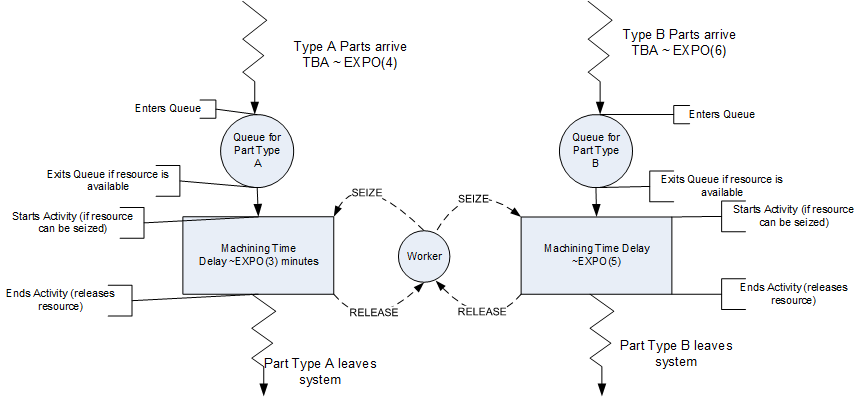
\includegraphics{./figures/ch5/SharedResource.png}
\caption{\label{fig:SharedResource}A Resource Shared Between Two Activities}
\end{figure}

How many events are there for the situation in Figure \ref{fig:SharedResource}? From the strict definition of an event, there are six events in this situation. There are the two arrival
events for each type of part. There are two different begin service
events and two different end service events. From an implementation
perspective, we could model this situation with only two events. We can
have a single event that handles both types of arrivals and a single end
service event that handles the departure of either type of part. The
reason we only need one end service event is because the begin service
event logic can be incorporated in the end of service event because whenever a
service completes a waiting part will start into service. How many
events should you use in your modeling? You should implement the events
in a way that facilitates your perspective and your modeling. The
trade-off is that when the event logic is consolidated, the logic may be
more complicated.

The following listing presents the constructor for the shared queue
example. Notice that two instances of the \texttt{Queue} and \texttt{EventGenerator}
classes are used. The two event generators are used to implement the
arrival processes for the two types of parts. The two queues are used to
hold the two types of parts. An instance of \texttt{SResource} is used to
represent the workers that are shared between the two activities. The
activity times are represented by two \texttt{RandomVariable} instances. A
\texttt{TimeWeighted} instance and a \texttt{ResponseVariable} instance are used to
collect statistics on the number of parts in the system and the time
spent in the system, respectively.

\begin{Shaded}
\begin{Highlighting}[]
\KeywordTok{public} \KeywordTok{class}\NormalTok{ SharedResource }\KeywordTok{extends}\NormalTok{ SchedulingElement }\OperatorTok{\{}

    \KeywordTok{private} \DataTypeTok{final}\NormalTok{ EventGenerator myTypeAGenerator}\OperatorTok{;}
    \KeywordTok{private} \DataTypeTok{final}\NormalTok{ EventGenerator myTypeBGenerator}\OperatorTok{;}
    \KeywordTok{private} \DataTypeTok{final}\NormalTok{ TimeWeighted myNumInSystem}\OperatorTok{;}
    \KeywordTok{private} \DataTypeTok{final}\NormalTok{ ResponseVariable mySystemTime}\OperatorTok{;}
    \KeywordTok{private} \DataTypeTok{final}\NormalTok{ SResource myServers}\OperatorTok{;}
    \KeywordTok{private} \DataTypeTok{final} \BuiltInTok{Queue}\OperatorTok{\textless{}}\NormalTok{QObject}\OperatorTok{\textgreater{}}\NormalTok{ myTypeAWaitingQ}\OperatorTok{;}
    \KeywordTok{private} \DataTypeTok{final} \BuiltInTok{Queue}\OperatorTok{\textless{}}\NormalTok{QObject}\OperatorTok{\textgreater{}}\NormalTok{ myTypeBWaitingQ}\OperatorTok{;}
    \KeywordTok{private} \DataTypeTok{final}\NormalTok{ EndServiceEventAction myEndServiceEventAction}\OperatorTok{;}
    \KeywordTok{private} \DataTypeTok{final}\NormalTok{ RandomVariable myServiceRVTypeA}\OperatorTok{;}
    \KeywordTok{private} \DataTypeTok{final}\NormalTok{ RandomVariable myServiceRVTypeB}\OperatorTok{;}
    
    \KeywordTok{public} \FunctionTok{SharedResource}\OperatorTok{(}\NormalTok{ModelElement parent}\OperatorTok{,} \DataTypeTok{int}\NormalTok{ numServers}\OperatorTok{,}\NormalTok{ RVariableIfc tbaA}\OperatorTok{,}
\NormalTok{                          RVariableIfc tbaB}\OperatorTok{,}\NormalTok{ RVariableIfc stA}\OperatorTok{,}\NormalTok{ RVariableIfc stB}\OperatorTok{,} \BuiltInTok{String}\NormalTok{ name}\OperatorTok{)} \OperatorTok{\{}
        \KeywordTok{super}\OperatorTok{(}\NormalTok{parent}\OperatorTok{,}\NormalTok{ name}\OperatorTok{);}
\NormalTok{        myTypeAGenerator }\OperatorTok{=} \KeywordTok{new} \FunctionTok{EventGenerator}\OperatorTok{(}\KeywordTok{this}\OperatorTok{,} \KeywordTok{new} \FunctionTok{TypeAArrivals}\OperatorTok{(),}\NormalTok{ tbaA}\OperatorTok{,}\NormalTok{ tbaA}\OperatorTok{);}
\NormalTok{        myTypeBGenerator }\OperatorTok{=} \KeywordTok{new} \FunctionTok{EventGenerator}\OperatorTok{(}\KeywordTok{this}\OperatorTok{,} \KeywordTok{new} \FunctionTok{TypeBArrivals}\OperatorTok{(),}\NormalTok{ tbaB}\OperatorTok{,}\NormalTok{ tbaB}\OperatorTok{);}
\NormalTok{        myServiceRVTypeA }\OperatorTok{=} \KeywordTok{new} \FunctionTok{RandomVariable}\OperatorTok{(}\KeywordTok{this}\OperatorTok{,}\NormalTok{ stA}\OperatorTok{,} \StringTok{"Service RV A"}\OperatorTok{);}
\NormalTok{        myServiceRVTypeB }\OperatorTok{=} \KeywordTok{new} \FunctionTok{RandomVariable}\OperatorTok{(}\KeywordTok{this}\OperatorTok{,}\NormalTok{ stB}\OperatorTok{,} \StringTok{"Service RV B"}\OperatorTok{);}
\NormalTok{        myServers }\OperatorTok{=} \KeywordTok{new} \FunctionTok{SResource}\OperatorTok{(}\KeywordTok{this}\OperatorTok{,}\NormalTok{ numServers}\OperatorTok{,} \StringTok{"Servers"}\OperatorTok{);}
\NormalTok{        myTypeAWaitingQ }\OperatorTok{=} \KeywordTok{new} \BuiltInTok{Queue}\OperatorTok{\textless{}\textgreater{}(}\KeywordTok{this}\OperatorTok{,} \FunctionTok{getName}\OperatorTok{()} \OperatorTok{+} \StringTok{"\_QA"}\OperatorTok{);}
\NormalTok{        myTypeBWaitingQ }\OperatorTok{=} \KeywordTok{new} \BuiltInTok{Queue}\OperatorTok{\textless{}\textgreater{}(}\KeywordTok{this}\OperatorTok{,} \FunctionTok{getName}\OperatorTok{()} \OperatorTok{+} \StringTok{"\_QB"}\OperatorTok{);}
\NormalTok{        mySystemTime }\OperatorTok{=} \KeywordTok{new} \FunctionTok{ResponseVariable}\OperatorTok{(}\KeywordTok{this}\OperatorTok{,} \StringTok{"System Time"}\OperatorTok{);}
\NormalTok{        myNumInSystem }\OperatorTok{=} \KeywordTok{new} \FunctionTok{TimeWeighted}\OperatorTok{(}\KeywordTok{this}\OperatorTok{,} \StringTok{"Num in System"}\OperatorTok{);}
\NormalTok{        myEndServiceEventAction }\OperatorTok{=} \KeywordTok{new} \FunctionTok{EndServiceEventAction}\OperatorTok{();}
    \OperatorTok{\}}
\end{Highlighting}
\end{Shaded}

The following listing presents the arrivals of the parts via the
generator listeners and the beginning of service. In line~5, the number
of parts is incremented. Then, in line~6, the arriving part is
represented with a new \texttt{QObject}, which is immediately enqueued. The if
statement starting at line~7, checks if the resource has available units
and if so, begins serving the next part. In the \texttt{serveNext()} method, the
two queues are checked. Notice that the queue for type A parts is
checked first. If the queue is not empty, then the part is removed and
started into service using the service time distribution for type A
parts. If there are no type A parts, the queue for type B parts is
checked in a similar fashion. Because the type A queue is checked first,
it will have priority over the type B part queue.

\begin{Shaded}
\begin{Highlighting}[]
    \KeywordTok{private} \KeywordTok{class}\NormalTok{ TypeAArrivals }\KeywordTok{implements}\NormalTok{ EventGeneratorActionIfc }\OperatorTok{\{}

        \AttributeTok{@Override}
        \KeywordTok{public} \DataTypeTok{void} \FunctionTok{generate}\OperatorTok{(}\NormalTok{EventGenerator generator}\OperatorTok{,}\NormalTok{ JSLEvent event}\OperatorTok{)} \OperatorTok{\{}
\NormalTok{            myNumInSystem}\OperatorTok{.}\FunctionTok{increment}\OperatorTok{();}
\NormalTok{            myTypeAWaitingQ}\OperatorTok{.}\FunctionTok{enqueue}\OperatorTok{(}\KeywordTok{new} \FunctionTok{QObject}\OperatorTok{(}\FunctionTok{getTime}\OperatorTok{()));}
            \ControlFlowTok{if} \OperatorTok{(}\NormalTok{myServers}\OperatorTok{.}\FunctionTok{hasAvailableUnits}\OperatorTok{())} \OperatorTok{\{} \CommentTok{// server available}
                \FunctionTok{serveNext}\OperatorTok{();}
            \OperatorTok{\}}
        \OperatorTok{\}}

    \OperatorTok{\}}

    \KeywordTok{private} \KeywordTok{class}\NormalTok{ TypeBArrivals }\KeywordTok{implements}\NormalTok{ EventGeneratorActionIfc }\OperatorTok{\{}

        \AttributeTok{@Override}
        \KeywordTok{public} \DataTypeTok{void} \FunctionTok{generate}\OperatorTok{(}\NormalTok{EventGenerator generator}\OperatorTok{,}\NormalTok{ JSLEvent event}\OperatorTok{)} \OperatorTok{\{}
\NormalTok{            myNumInSystem}\OperatorTok{.}\FunctionTok{increment}\OperatorTok{();}
\NormalTok{            myTypeBWaitingQ}\OperatorTok{.}\FunctionTok{enqueue}\OperatorTok{(}\KeywordTok{new} \FunctionTok{QObject}\OperatorTok{(}\FunctionTok{getTime}\OperatorTok{()));}
            \ControlFlowTok{if} \OperatorTok{(}\NormalTok{myServers}\OperatorTok{.}\FunctionTok{hasAvailableUnits}\OperatorTok{())} \OperatorTok{\{} \CommentTok{// server available}
                \FunctionTok{serveNext}\OperatorTok{();}
            \OperatorTok{\}}
        \OperatorTok{\}}

    \OperatorTok{\}}

    \KeywordTok{private} \DataTypeTok{void} \FunctionTok{serveNext}\OperatorTok{()} \OperatorTok{\{}
        \CommentTok{//logic to choose next from queues}
        \CommentTok{// if both have waiting parts, assume part type A has priority}
        \ControlFlowTok{if} \OperatorTok{(}\NormalTok{myTypeAWaitingQ}\OperatorTok{.}\FunctionTok{isNotEmpty}\OperatorTok{())} \OperatorTok{\{}
\NormalTok{            QObject partA }\OperatorTok{=}\NormalTok{ myTypeAWaitingQ}\OperatorTok{.}\FunctionTok{removeNext}\OperatorTok{();} \CommentTok{//remove the next customer}
\NormalTok{            myServers}\OperatorTok{.}\FunctionTok{seize}\OperatorTok{();}
            \CommentTok{// schedule end of service}
            \FunctionTok{scheduleEvent}\OperatorTok{(}\NormalTok{myEndServiceEventAction}\OperatorTok{,}\NormalTok{ myServiceRVTypeA}\OperatorTok{,}\NormalTok{ partA}\OperatorTok{);}
        \OperatorTok{\}} \ControlFlowTok{else} \ControlFlowTok{if} \OperatorTok{(}\NormalTok{myTypeBWaitingQ}\OperatorTok{.}\FunctionTok{isNotEmpty}\OperatorTok{())} \OperatorTok{\{}
\NormalTok{            QObject partB }\OperatorTok{=}\NormalTok{ myTypeBWaitingQ}\OperatorTok{.}\FunctionTok{removeNext}\OperatorTok{();} \CommentTok{//remove the next customer}
\NormalTok{            myServers}\OperatorTok{.}\FunctionTok{seize}\OperatorTok{();}
            \CommentTok{// schedule end of service}
            \FunctionTok{scheduleEvent}\OperatorTok{(}\NormalTok{myEndServiceEventAction}\OperatorTok{,}\NormalTok{ myServiceRVTypeB}\OperatorTok{,}\NormalTok{ partB}\OperatorTok{);}
        \OperatorTok{\}}
    \OperatorTok{\}}
\end{Highlighting}
\end{Shaded}

The following code listing presents the end of service event logic for the
shared resource example. The end of service logic is very similar to
logic that we have seen for the departure from a queueing station. In
the end of service action, the part that is leaving is passed to the
outer class for statistical collection in the \texttt{departingSystem()} method.
The resource is released and the queues are checked to see if a part is
waiting. Note that both queues are checked, such that if either queue
has a waiting part, the logic for serving the next part is invoked.

\begin{Shaded}
\begin{Highlighting}[]
    \KeywordTok{private} \DataTypeTok{boolean} \FunctionTok{checkQueues}\OperatorTok{()} \OperatorTok{\{}
        \ControlFlowTok{return} \OperatorTok{(}\NormalTok{myTypeAWaitingQ}\OperatorTok{.}\FunctionTok{isNotEmpty}\OperatorTok{()} \OperatorTok{||}\NormalTok{ myTypeBWaitingQ}\OperatorTok{.}\FunctionTok{isNotEmpty}\OperatorTok{());}
    \OperatorTok{\}}

    \KeywordTok{private} \KeywordTok{class}\NormalTok{ EndServiceEventAction }\KeywordTok{implements}\NormalTok{ EventActionIfc}\OperatorTok{\textless{}}\NormalTok{QObject}\OperatorTok{\textgreater{}} \OperatorTok{\{}

        \AttributeTok{@Override}
        \KeywordTok{public} \DataTypeTok{void} \FunctionTok{action}\OperatorTok{(}\NormalTok{JSLEvent}\OperatorTok{\textless{}}\NormalTok{QObject}\OperatorTok{\textgreater{}}\NormalTok{ event}\OperatorTok{)} \OperatorTok{\{}
\NormalTok{            QObject leavingPart }\OperatorTok{=}\NormalTok{ event}\OperatorTok{.}\FunctionTok{getMessage}\OperatorTok{();}
\NormalTok{            myServers}\OperatorTok{.}\FunctionTok{release}\OperatorTok{();}
            \ControlFlowTok{if} \OperatorTok{(}\FunctionTok{checkQueues}\OperatorTok{())} \OperatorTok{\{} \CommentTok{// queue is not empty}
                \FunctionTok{serveNext}\OperatorTok{();}
            \OperatorTok{\}}
            \FunctionTok{departSystem}\OperatorTok{(}\NormalTok{leavingPart}\OperatorTok{);}
        \OperatorTok{\}}
    \OperatorTok{\}}

    \KeywordTok{private} \DataTypeTok{void} \FunctionTok{departSystem}\OperatorTok{(}\NormalTok{QObject leavingPart}\OperatorTok{)} \OperatorTok{\{}
\NormalTok{        mySystemTime}\OperatorTok{.}\FunctionTok{setValue}\OperatorTok{(}\FunctionTok{getTime}\OperatorTok{()} \OperatorTok{{-}}\NormalTok{ leavingPart}\OperatorTok{.}\FunctionTok{getCreateTime}\OperatorTok{());}
\NormalTok{        myNumInSystem}\OperatorTok{.}\FunctionTok{decrement}\OperatorTok{();} \CommentTok{// part left system      }
    \OperatorTok{\}}
\end{Highlighting}
\end{Shaded}

Finally, the following code shows how to setup and run the example. The system is configured with the time between arrivals for type A parts and type B parts having exponential distributions with
means of 4 and 6 time units, respectively. The service time
distributions are also exponential with means of 3 and 5, respectively
for type A and B parts. The capacity of the resource is set at 2
workers.

\begin{Shaded}
\begin{Highlighting}[]
    \KeywordTok{public} \DataTypeTok{static} \DataTypeTok{void} \FunctionTok{main}\OperatorTok{(}\BuiltInTok{String}\OperatorTok{[]}\NormalTok{ args}\OperatorTok{)} \OperatorTok{\{}
\NormalTok{        Simulation sim }\OperatorTok{=} \KeywordTok{new} \FunctionTok{Simulation}\OperatorTok{(}\StringTok{"Shared Resource Example"}\OperatorTok{);}
        \CommentTok{// get the model}
\NormalTok{        Model m }\OperatorTok{=}\NormalTok{ sim}\OperatorTok{.}\FunctionTok{getModel}\OperatorTok{();}
        \CommentTok{// add to the main model}
\NormalTok{        RVariableIfc tbaA }\OperatorTok{=} \KeywordTok{new} \FunctionTok{ExponentialRV}\OperatorTok{(}\FloatTok{4.0}\OperatorTok{);}
\NormalTok{        RVariableIfc tbaB }\OperatorTok{=} \KeywordTok{new} \FunctionTok{ExponentialRV}\OperatorTok{(}\FloatTok{6.0}\OperatorTok{);}
\NormalTok{        RVariableIfc stA }\OperatorTok{=} \KeywordTok{new} \FunctionTok{ExponentialRV}\OperatorTok{(}\FloatTok{3.0}\OperatorTok{);}
\NormalTok{        RVariableIfc stB }\OperatorTok{=} \KeywordTok{new} \FunctionTok{ExponentialRV}\OperatorTok{(}\FloatTok{5.0}\OperatorTok{);}
\NormalTok{        SharedResource sr }\OperatorTok{=} \KeywordTok{new} \FunctionTok{SharedResource}\OperatorTok{(}\NormalTok{m}\OperatorTok{,} \DecValTok{2}\OperatorTok{,}\NormalTok{ tbaA}\OperatorTok{,}\NormalTok{ tbaB}\OperatorTok{,}\NormalTok{ stA}\OperatorTok{,}\NormalTok{ stB}\OperatorTok{,} \StringTok{"SR"}\OperatorTok{);}
        \CommentTok{// set the parameters of the experiment}
\NormalTok{        sim}\OperatorTok{.}\FunctionTok{setNumberOfReplications}\OperatorTok{(}\DecValTok{30}\OperatorTok{);}
\NormalTok{        sim}\OperatorTok{.}\FunctionTok{setLengthOfReplication}\OperatorTok{(}\FloatTok{20000.0}\OperatorTok{);}
\NormalTok{        sim}\OperatorTok{.}\FunctionTok{setLengthOfWarmUp}\OperatorTok{(}\FloatTok{5000.0}\OperatorTok{);}
\NormalTok{        SimulationReporter r }\OperatorTok{=}\NormalTok{ sim}\OperatorTok{.}\FunctionTok{makeSimulationReporter}\OperatorTok{();}
        \BuiltInTok{System}\OperatorTok{.}\FunctionTok{out}\OperatorTok{.}\FunctionTok{println}\OperatorTok{(}\StringTok{"Simulation started."}\OperatorTok{);}
\NormalTok{        sim}\OperatorTok{.}\FunctionTok{run}\OperatorTok{();}
        \BuiltInTok{System}\OperatorTok{.}\FunctionTok{out}\OperatorTok{.}\FunctionTok{println}\OperatorTok{(}\StringTok{"Simulation completed."}\OperatorTok{);}
\NormalTok{        r}\OperatorTok{.}\FunctionTok{printAcrossReplicationSummaryStatistics}\OperatorTok{();}
    \OperatorTok{\}}
\end{Highlighting}
\end{Shaded}

The results indicate that the type B parts wait
significantly longer on average than the type A parts. It should be
apparent that with some additional design that the shared resource
example could be generalized into a class that could be used in other
simulation models similar to how the single station queue has been
generalized. This is one of the important advantages of an
object-oriented approach to simulation modeling.

\begin{longtable}[]{@{}
  >{\centering\arraybackslash}p{(\columnwidth - 0\tabcolsep) * \real{1.00}}@{}}
\toprule
\endhead
\begin{minipage}[t]{\linewidth}\raggedright
\hypertarget{fig:RSOutput}{%
\label{fig:RSOutput}}%
\begin{verbatim}
Number of Replications: 30
Length of Warm up period: 5000.0
Length of Replications: 20000.0
---------------------------------------------------------------------
----
Response Variables
---------------------------------------------------------------------
----
Name                              Average       Std. Dev.       Count

---------------------------------------------------------------------
----
Servers_Util                     0.792550        0.015226       30.00
0000
Servers_#Busy Units              1.585100        0.030453       30.00
0000
SR_QA : Number In Q              0.589924        0.044712       30.00
0000
SR_QA : Time In Q                2.361027        0.155425       30.00
0000
SR_QB : Number In Q              1.948387        0.363318       30.00
0000
SR_QB : Time In Q               11.664922        2.087974       30.00
0000
System Time                      9.891819        0.908085       30.00
0000
Num in System                    4.123410        0.413465       30.00
0000
---------------------------------------------------------------------
----
\end{verbatim}
\end{minipage} \\
\bottomrule
\end{longtable}

\hypertarget{dem:tiedyeShirts}{%
\section{Complex System Example}\label{dem:tiedyeShirts}}

This section presents a more complex system that illustrates how to
model entities that flow through a system and how to coordinate the
flow. The example will reuse the single queue station modeling of
previous examples; however, the entities (objects that flow in the
system) require synchronization.

Suppose production orders for tie-dye T-shirts arrive to a production
facility according to a Poisson process with a mean rate of 4 per hour.
There are two basic psychedelic designs involving either red or blue
dye. For some reason the blue shirts are a little more popular than the
red shirts so that when an order arrives about 70\% of the time it is for
the blue dye designs. In addition, there are two different package sizes
for the shirts, 3 and 5 units. There is a 25\% chance that the order will
be for a package size of 5 and a 75\% chance that the order will be for a
package size of 3. Each of the shirts must be \emph{individually} hand made
to the customer's order design specifications. The time to produce a
shirt (of either color) is uniformly distributed within the range of 3
to 5 minutes. There is currently one worker who is setup to make either
shirt. When an order arrives to the facility, its type (red or blue) is
determined and the pack size is determined. Then, the appropriate number
of white (un-dyed) shirts are sent to the shirt makers with a note
pinned to the shirt indicating the customer order, its basic design, and
the pack size for the order. Meanwhile, the paperwork for the order is
processed by a worker and a customized packaging letter and box is
prepared to hold the order. It takes the paperwork worker between 8 to
10 minutes to make the box and print a custom thank you note. After the
packaging is made the paperwork waits prior to final inspection for the
shirts associated with the order. After the shirts are combined with the
packaging, they are inspected by a packaging worker which is distributed
according to a triangular distribution with a minimum of 5 minutes, a
most likely value of 10 minutes, and a maximum value of 15 minutes.
Finally, the boxed customer order is sent to shipping.

\hypertarget{dem:tiedyeShirts:cm}{%
\subsection{Conceptualizing the Model}\label{dem:tiedyeShirts:cm}}

Before proceeding you might want to jot down your answers to the
following modeling recipe questions and then compare how you are doing
with respect to what is presented in this section. The modeling recipe
questions are:

\begin{itemize}
\item
  What is the system? What information is known by the system?
\item
  What are the required performance measures?
\item
  What are the entities? What information must be recorded or
  remembered for each entity? How are entities introduced into the
  system?
\item
  What are the resources that are used by the entities? Which entities
  use which resources and how?
\item
  What are the process flows? Sketch the process or make an activity
  flow diagram
\item
  Develop pseudo-code for the situation
\item
  Implement the model
\end{itemize}

The entities can be conceptualized as the arriving orders. Since the
shirts are processed individually, they should also be considered
entities. In addition, the type of order (red or blue) and the size of
the order (3 or 5) must be tracked. Since the type of the order and the
size of the order are properties of the order, attributes can be used to
model this information. The resources are the two shirt makers, the
paperwork worker, and the packager. The flow is described in the
scenario statement: orders arrive, shirts made, meanwhile packaging is
made. Then, orders are assembled, inspected, and finally shipped. It
should be clear that an EventGenerator, setup to generate Poisson
arrivals can create the orders, but if shirts are entities, how should
they be modeled and created? After this, there will be two types of
entities in the model, the orders (paperwork) and the shirts. The shirts
can be made and meanwhile the paperwork for the order can be processed.
When the shirts for an order are made, they need to be combined together
and associated with the order.

The activity diagram for this situation is given in Figure \ref{fig:TieDyeTShirtACD}. After the order is created, the process separates into the order making process and the shirt making
process. Notice that the orders and shirts must be synchronized together
after each of these processes.

\begin{figure}
\centering
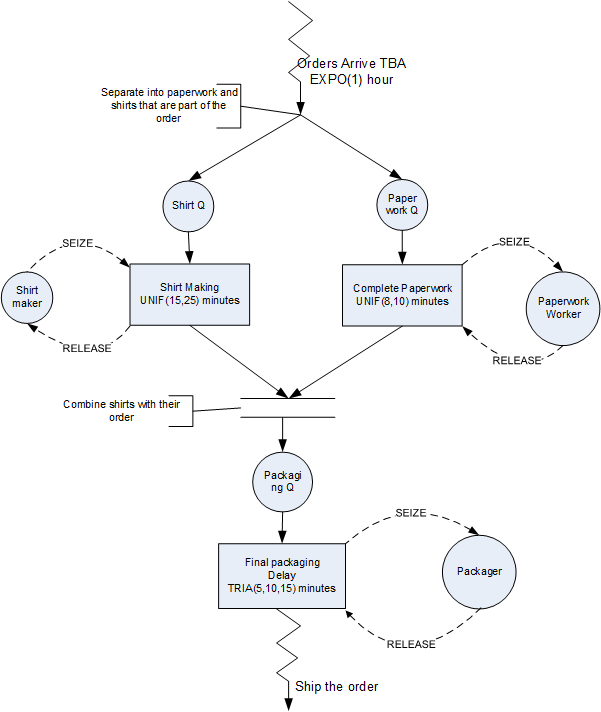
\includegraphics{./figures/ch5/TieDyeTShirtACD.png}
\caption{\label{fig:TieDyeTShirtACD}Activity Diagram for Tie Dye T-Shirts System}
\end{figure}

\hypertarget{dem:tiedyeShirts:im}{%
\subsection{Implementing the Model}\label{dem:tiedyeShirts:im}}

If it was not for the coordination between the orders
(paperwork/packaging) and the shirts in this system, the modeling would
be a straightforward application of concepts that have already been
presented. The processing of the shirts, the paperwork, and the final
packaging can all be modeled with instances of the \texttt{SingleQueueStation}
class, where the shirts go to one instance, the paperwork goes to
another instance, and the combined final order goes to the third
instance. Thus, if it was not for the fact that shirts must be combined
into an order and the order has to be combined with its paperwork before
packaging, the classes within the station package could handle this
modeling. In fact, the constructor for the implementation takes exactly
this approach as illustrated in the following code listing.

\begin{Shaded}
\begin{Highlighting}[]
    \KeywordTok{public} \FunctionTok{TieDyeTShirts}\OperatorTok{(}\NormalTok{ModelElement parent}\OperatorTok{,} \BuiltInTok{String}\NormalTok{ name}\OperatorTok{)} \OperatorTok{\{}
        \KeywordTok{super}\OperatorTok{(}\NormalTok{parent}\OperatorTok{,}\NormalTok{ name}\OperatorTok{);}
\NormalTok{        myTBOrders }\OperatorTok{=} \KeywordTok{new} \FunctionTok{RandomVariable}\OperatorTok{(}\KeywordTok{this}\OperatorTok{,} \KeywordTok{new} \FunctionTok{ExponentialRV}\OperatorTok{(}\DecValTok{15}\OperatorTok{));}
\NormalTok{        myOrderGenerator }\OperatorTok{=} \KeywordTok{new} \FunctionTok{EventGenerator}\OperatorTok{(}\KeywordTok{this}\OperatorTok{,} \KeywordTok{new} \FunctionTok{OrderArrivals}\OperatorTok{(),}
\NormalTok{                myTBOrders}\OperatorTok{,}\NormalTok{ myTBOrders}\OperatorTok{);}
\NormalTok{        DEmpiricalRV type }\OperatorTok{=} \KeywordTok{new} \FunctionTok{DEmpiricalRV}\OperatorTok{(}\KeywordTok{new} \DataTypeTok{double}\OperatorTok{[]\{}\FloatTok{1.0}\OperatorTok{,} \FloatTok{2.0}\OperatorTok{\},} \KeywordTok{new} \DataTypeTok{double}\OperatorTok{[]} \OperatorTok{\{}\FloatTok{0.7}\OperatorTok{,} \FloatTok{1.0}\OperatorTok{\});}
\NormalTok{        DEmpiricalRV size }\OperatorTok{=} \KeywordTok{new} \FunctionTok{DEmpiricalRV}\OperatorTok{(}\KeywordTok{new} \DataTypeTok{double}\OperatorTok{[]\{}\FloatTok{3.0}\OperatorTok{,} \FloatTok{5.0}\OperatorTok{\},} \KeywordTok{new} \DataTypeTok{double}\OperatorTok{[]} \OperatorTok{\{}\FloatTok{0.75}\OperatorTok{,} \FloatTok{1.0}\OperatorTok{\});}
\NormalTok{        myOrderSize }\OperatorTok{=} \KeywordTok{new} \FunctionTok{RandomVariable}\OperatorTok{(}\KeywordTok{this}\OperatorTok{,}\NormalTok{ size}\OperatorTok{);}
\NormalTok{        myOrderType }\OperatorTok{=} \KeywordTok{new} \FunctionTok{RandomVariable}\OperatorTok{(}\KeywordTok{this}\OperatorTok{,}\NormalTok{ type}\OperatorTok{);}
\NormalTok{        myShirtMakingTime }\OperatorTok{=} \KeywordTok{new} \FunctionTok{RandomVariable}\OperatorTok{(}\KeywordTok{this}\OperatorTok{,} \KeywordTok{new} \FunctionTok{UniformRV}\OperatorTok{(}\DecValTok{3}\OperatorTok{,} \DecValTok{5}\OperatorTok{));}
\NormalTok{        myPaperWorkTime }\OperatorTok{=} \KeywordTok{new} \FunctionTok{RandomVariable}\OperatorTok{(}\KeywordTok{this}\OperatorTok{,} \KeywordTok{new} \FunctionTok{UniformRV}\OperatorTok{(}\DecValTok{8}\OperatorTok{,} \DecValTok{10}\OperatorTok{));}
\NormalTok{        myPackagingTime }\OperatorTok{=} \KeywordTok{new} \FunctionTok{RandomVariable}\OperatorTok{(}\KeywordTok{this}\OperatorTok{,} \KeywordTok{new} \FunctionTok{TriangularRV}\OperatorTok{(}\DecValTok{5}\OperatorTok{,} \DecValTok{10}\OperatorTok{,} \DecValTok{15}\OperatorTok{));}
\NormalTok{        myShirtMakers }\OperatorTok{=} \KeywordTok{new} \FunctionTok{SResource}\OperatorTok{(}\KeywordTok{this}\OperatorTok{,} \DecValTok{1}\OperatorTok{,} \StringTok{"ShirtMakers\_R"}\OperatorTok{);}
\NormalTok{        myPackager }\OperatorTok{=} \KeywordTok{new} \FunctionTok{SResource}\OperatorTok{(}\KeywordTok{this}\OperatorTok{,} \DecValTok{1}\OperatorTok{,} \StringTok{"Packager\_R"}\OperatorTok{);}
\NormalTok{        myShirtMakingStation }\OperatorTok{=} \KeywordTok{new} \FunctionTok{SingleQueueStation}\OperatorTok{(}\KeywordTok{this}\OperatorTok{,}\NormalTok{ myShirtMakers}\OperatorTok{,}
\NormalTok{                myShirtMakingTime}\OperatorTok{,} \StringTok{"Shirt\_Station"}\OperatorTok{);}
\NormalTok{        myWorker }\OperatorTok{=} \KeywordTok{new} \FunctionTok{SResource}\OperatorTok{(}\KeywordTok{this}\OperatorTok{,} \DecValTok{1}\OperatorTok{,} \StringTok{"PW{-}Worker"}\OperatorTok{);}
\NormalTok{        myPWStation }\OperatorTok{=} \KeywordTok{new} \FunctionTok{SingleQueueStation}\OperatorTok{(}\KeywordTok{this}\OperatorTok{,}\NormalTok{ myWorker}\OperatorTok{,}
\NormalTok{                myPaperWorkTime}\OperatorTok{,} \StringTok{"PW\_Station"}\OperatorTok{);}
\NormalTok{        myPackagingStation }\OperatorTok{=} \KeywordTok{new} \FunctionTok{SingleQueueStation}\OperatorTok{(}\KeywordTok{this}\OperatorTok{,}\NormalTok{ myPackager}\OperatorTok{,}
\NormalTok{                myPackagingTime}\OperatorTok{,} \StringTok{"Packing\_Station"}\OperatorTok{);}
        \CommentTok{// need to set senders/receivers}
\NormalTok{        myShirtMakingStation}\OperatorTok{.}\FunctionTok{setNextReceiver}\OperatorTok{(}\KeywordTok{new} \FunctionTok{AfterShirtMaking}\OperatorTok{());}
\NormalTok{        myPWStation}\OperatorTok{.}\FunctionTok{setNextReceiver}\OperatorTok{(}\KeywordTok{new} \FunctionTok{AfterPaperWork}\OperatorTok{());}
\NormalTok{        myPackagingStation}\OperatorTok{.}\FunctionTok{setNextReceiver}\OperatorTok{(}\KeywordTok{new} \FunctionTok{Dispose}\OperatorTok{());}
\NormalTok{        mySystemTime }\OperatorTok{=} \KeywordTok{new} \FunctionTok{ResponseVariable}\OperatorTok{(}\KeywordTok{this}\OperatorTok{,} \StringTok{"System Time"}\OperatorTok{);}
\NormalTok{        myNumInSystem }\OperatorTok{=} \KeywordTok{new} \FunctionTok{TimeWeighted}\OperatorTok{(}\KeywordTok{this}\OperatorTok{,} \StringTok{"Num in System"}\OperatorTok{);}
    \OperatorTok{\}}
\end{Highlighting}
\end{Shaded}

In the constructor, lines~3 and 4, shows the
specification for the \texttt{EventGenerator.} Then, \texttt{DEmpiricalRV} random
variables are setup to model the order size and the order type, where 1
represents blue shirts and 2 represents red shirts. Lines~10-12 show the
modeling of the shirt making time, paperwork time, and packaging time
all using instances of the \texttt{RandomVariable} class. In lines~13-15 the
workers are modeled with instances of the \texttt{SResource} class, and in
lines~16-21, the \texttt{SingleQueueStation} class is used to model the use of
the resources and the activities for shirt making, paperwork, and
packaging. All that is left is connecting the stations together, which
is accomplished in lines~23-25 by setting the receivers for the
stations. The `magic' of modeling the order coordination happens in the
receivers and how orders are modeled.

Before exploring that implementation, we can explore how orders enter
and leave the system. The following listing presents how the orders are generated and how
the orders leave the system.

\begin{Shaded}
\begin{Highlighting}[]
    \KeywordTok{private} \KeywordTok{class}\NormalTok{ OrderArrivals }\KeywordTok{implements}\NormalTok{ EventGeneratorActionIfc }\OperatorTok{\{}

        \AttributeTok{@Override}
        \KeywordTok{public} \DataTypeTok{void} \FunctionTok{generate}\OperatorTok{(}\NormalTok{EventGenerator generator}\OperatorTok{,}\NormalTok{ JSLEvent event}\OperatorTok{)} \OperatorTok{\{}
\NormalTok{            myNumInSystem}\OperatorTok{.}\FunctionTok{increment}\OperatorTok{();}
\NormalTok{            Order order }\OperatorTok{=} \KeywordTok{new} \FunctionTok{Order}\OperatorTok{();}
            \BuiltInTok{List}\OperatorTok{\textless{}}\NormalTok{Order}\OperatorTok{.}\FunctionTok{Shirt}\OperatorTok{\textgreater{}}\NormalTok{ shirts }\OperatorTok{=}\NormalTok{ order}\OperatorTok{.}\FunctionTok{getShirts}\OperatorTok{();}

            \ControlFlowTok{for} \OperatorTok{(}\NormalTok{Order}\OperatorTok{.}\FunctionTok{Shirt}\NormalTok{ shirt }\OperatorTok{:}\NormalTok{ shirts}\OperatorTok{)} \OperatorTok{\{}
\NormalTok{                myShirtMakingStation}\OperatorTok{.}\FunctionTok{receive}\OperatorTok{(}\NormalTok{shirt}\OperatorTok{);}
            \OperatorTok{\}}
\NormalTok{            myPWStation}\OperatorTok{.}\FunctionTok{receive}\OperatorTok{(}\NormalTok{order}\OperatorTok{.}\FunctionTok{getPaperWork}\OperatorTok{());}

        \OperatorTok{\}}

    \OperatorTok{\}}

    \KeywordTok{protected} \KeywordTok{class}\NormalTok{ Dispose }\KeywordTok{implements}\NormalTok{ ReceiveQObjectIfc }\OperatorTok{\{}

        \AttributeTok{@Override}
        \KeywordTok{public} \DataTypeTok{void} \FunctionTok{receive}\OperatorTok{(}\NormalTok{QObject qObj}\OperatorTok{)} \OperatorTok{\{}
            \CommentTok{// collect final statistics}
\NormalTok{            myNumInSystem}\OperatorTok{.}\FunctionTok{decrement}\OperatorTok{();}
\NormalTok{            mySystemTime}\OperatorTok{.}\FunctionTok{setValue}\OperatorTok{(}\FunctionTok{getTime}\OperatorTok{()} \OperatorTok{{-}}\NormalTok{ qObj}\OperatorTok{.}\FunctionTok{getCreateTime}\OperatorTok{());}
\NormalTok{            Order o }\OperatorTok{=} \OperatorTok{(}\NormalTok{Order}\OperatorTok{)}\NormalTok{ qObj}\OperatorTok{;}
\NormalTok{            o}\OperatorTok{.}\FunctionTok{dispose}\OperatorTok{();}
        \OperatorTok{\}}

    \OperatorTok{\}}
\end{Highlighting}
\end{Shaded}

An implementation of an \texttt{EventGeneratorListenerIfc} interface called \texttt{OrderArrivals} is provided to
the \texttt{EventGenerator.} In line~5, the number of orders in the system is
incremented. Then, in line~6, a new order is made. The shirts associated
with the orders are then retrieved (line~7) and then sent to the shirt
making station (lines~9-11). Finally, line 12 retrieves the paperwork
from the order (\texttt{order.getPaperWork()}) and sends it to the paperwork
station. The implementation of the logic for orders to leave the system
is implemented in similar disposal logic as we have previously seen
(atarting at line 18). First, the number of orders is decremented and
the time that an order spent in the system collected. Then, the order is
disposed.

The modeling of the synchronization of the shirts and the paperwork
comes down to the following fact: when all the shirts are completed and
the paperwork is completed, then the order is completed and can be sent
to the packaging station. If the paperwork activity finishes before all
the shirts are completed, the order will be completed when the last
shirt is done. If all the shirts are completed before the paperwork is
completed, then the order waits until the paperwork is done. Thus, when
a shirt associated with an order is completed, we can check if the paper
work is done and if all shirts are done, the order can proceed. When the
paperwork is completed, we need to check if all shirts are done and if
so the order can proceed. Both shirt completion and paperwork completion
are events and these events are modeled within the \texttt{SingleQueueStation}
class. However, right after the events occur the \texttt{SingleQueueStation}
class uses its attached \texttt{QObjectReceiverIfc} instance. The logic for
checking for order completion can be added to the receivers. This logic
is presented in the following listing.

\begin{Shaded}
\begin{Highlighting}[]
    \KeywordTok{protected} \KeywordTok{class}\NormalTok{ AfterShirtMaking }\KeywordTok{implements}\NormalTok{ ReceiveQObjectIfc }\OperatorTok{\{}

        \AttributeTok{@Override}
        \KeywordTok{public} \DataTypeTok{void} \FunctionTok{receive}\OperatorTok{(}\NormalTok{QObject qObj}\OperatorTok{)} \OperatorTok{\{}
\NormalTok{            Order}\OperatorTok{.}\FunctionTok{Shirt}\NormalTok{ shirt }\OperatorTok{=} \OperatorTok{(}\NormalTok{Order}\OperatorTok{.}\FunctionTok{Shirt}\OperatorTok{)}\NormalTok{ qObj}\OperatorTok{;}
\NormalTok{            shirt}\OperatorTok{.}\FunctionTok{setDoneFlag}\OperatorTok{();}
        \OperatorTok{\}}

    \OperatorTok{\}}

    \KeywordTok{protected} \KeywordTok{class}\NormalTok{ AfterPaperWork }\KeywordTok{implements}\NormalTok{ ReceiveQObjectIfc }\OperatorTok{\{}

        \AttributeTok{@Override}
        \KeywordTok{public} \DataTypeTok{void} \FunctionTok{receive}\OperatorTok{(}\NormalTok{QObject qObj}\OperatorTok{)} \OperatorTok{\{}
\NormalTok{            Order}\OperatorTok{.}\FunctionTok{PaperWork}\NormalTok{ pw }\OperatorTok{=} \OperatorTok{(}\NormalTok{Order}\OperatorTok{.}\FunctionTok{PaperWork}\OperatorTok{)}\NormalTok{ qObj}\OperatorTok{;}
\NormalTok{            pw}\OperatorTok{.}\FunctionTok{setDoneFlag}\OperatorTok{();}
        \OperatorTok{\}}

    \OperatorTok{\}}
\end{Highlighting}
\end{Shaded}

Because of how the Order class is
implemented, this logic is not particularly interesting. As shown in the
code listing, all that occurs is to indicate the the shirt is completed
(line~6) and that the paperwork is completed (line~16). The Order class
is implemented such that it is notified whenever a shirt is completed
and when the paperwork is completed. If during this notification
process, the entire order is completed, the order will be sent to the
packaging station. This is the logic that we will explore next.

Because orders may need to wait, we are going to model them by
sub-classing from the \texttt{QObject} class. This allows the use of the \texttt{Queue}
class. In addition, shirts and paperwork are also entities that wait.
So, they will also be modeled as sub-classes of the \texttt{QObject} class.
Orders have a size and a type. In addition, orders contain shirts and
paperwork.The following listing shows the constructor and instance variables
for the Order class.

\begin{Shaded}
\begin{Highlighting}[]
    \KeywordTok{private} \KeywordTok{class}\NormalTok{ Order }\KeywordTok{extends}\NormalTok{ QObject }\OperatorTok{\{}

        \KeywordTok{private} \DataTypeTok{int}\NormalTok{ myType}\OperatorTok{;}
        \KeywordTok{private} \DataTypeTok{int}\NormalTok{ mySize}\OperatorTok{;}
        \KeywordTok{private}\NormalTok{ PaperWork myPaperWork}\OperatorTok{;}
        \KeywordTok{private} \BuiltInTok{List}\OperatorTok{\textless{}}\NormalTok{Shirt}\OperatorTok{\textgreater{}}\NormalTok{ myShirts}\OperatorTok{;}
        \KeywordTok{private} \DataTypeTok{int}\NormalTok{ myNumCompleted}\OperatorTok{;}
        \KeywordTok{private} \DataTypeTok{boolean}\NormalTok{ myPaperWorkDone}\OperatorTok{;}

        \KeywordTok{public} \FunctionTok{Order}\OperatorTok{(}\DataTypeTok{double}\NormalTok{ creationTime}\OperatorTok{,} \BuiltInTok{String}\NormalTok{ name}\OperatorTok{)} \OperatorTok{\{}
            \KeywordTok{super}\OperatorTok{(}\NormalTok{creationTime}\OperatorTok{,}\NormalTok{ name}\OperatorTok{);}
\NormalTok{            myNumCompleted }\OperatorTok{=} \DecValTok{0}\OperatorTok{;}
\NormalTok{            myPaperWorkDone }\OperatorTok{=} \KeywordTok{false}\OperatorTok{;}
\NormalTok{            myType }\OperatorTok{=} \OperatorTok{(}\DataTypeTok{int}\OperatorTok{)}\NormalTok{ myOrderType}\OperatorTok{.}\FunctionTok{getValue}\OperatorTok{();}
\NormalTok{            mySize }\OperatorTok{=} \OperatorTok{(}\DataTypeTok{int}\OperatorTok{)}\NormalTok{ myOrderSize}\OperatorTok{.}\FunctionTok{getValue}\OperatorTok{();}
\NormalTok{            myShirts }\OperatorTok{=} \KeywordTok{new} \BuiltInTok{ArrayList}\OperatorTok{\textless{}\textgreater{}();}
            \ControlFlowTok{for} \OperatorTok{(}\DataTypeTok{int}\NormalTok{ i }\OperatorTok{=} \DecValTok{1}\OperatorTok{;}\NormalTok{ i }\OperatorTok{\textless{}=}\NormalTok{ mySize}\OperatorTok{;}\NormalTok{ i}\OperatorTok{++)} \OperatorTok{\{}
\NormalTok{                myShirts}\OperatorTok{.}\FunctionTok{add}\OperatorTok{(}\KeywordTok{new} \FunctionTok{Shirt}\OperatorTok{());}
            \OperatorTok{\}}
\NormalTok{            myPaperWork }\OperatorTok{=} \KeywordTok{new} \FunctionTok{PaperWork}\OperatorTok{();}
        \OperatorTok{\}}
\end{Highlighting}
\end{Shaded}

The \texttt{Order} class is a private inner class of the
\texttt{TieDyeTShirts} class. This allows orders access to all the instance
variables and methods of the \texttt{TieDyeTShirts} class. It is declared private
since its usage is only within the \texttt{TieDyeTShirts} class. \texttt{Order} extends
\texttt{QObject} and has instance variables to represent the type and size of the
orders (lines~3 and 4). Lines~5 and 6 represent the associations between
the order and its shirts (held in a list) and its paperwork. In the
constructor body, the type and size are set from the random variables
declared in the \texttt{TieDyeTShirts} class. In addition, a list holding the
shirts is filled and the paperwork is created. The number of completed
shirts is noted as zero and the fact that the paperwork is not completed
is saved in an attribute.

The following listing illustrates the key methods associated with
modeling the behavior of the orders.

\begin{Shaded}
\begin{Highlighting}[]
        \KeywordTok{public} \DataTypeTok{boolean} \FunctionTok{isComplete}\OperatorTok{()} \OperatorTok{\{}
            \ControlFlowTok{return} \OperatorTok{((}\FunctionTok{areShirtsDone}\OperatorTok{())} \OperatorTok{\&\&} \OperatorTok{(}\FunctionTok{isPaperWorkDone}\OperatorTok{()));}
        \OperatorTok{\}}

        \KeywordTok{public} \DataTypeTok{boolean} \FunctionTok{areShirtsDone}\OperatorTok{()} \OperatorTok{\{}
            \ControlFlowTok{return} \OperatorTok{(}\NormalTok{myNumCompleted }\OperatorTok{==}\NormalTok{ mySize}\OperatorTok{);}
        \OperatorTok{\}}

        \KeywordTok{public} \DataTypeTok{boolean} \FunctionTok{isPaperWorkDone}\OperatorTok{()} \OperatorTok{\{}
            \ControlFlowTok{return} \OperatorTok{(}\NormalTok{myPaperWorkDone}\OperatorTok{);}
        \OperatorTok{\}}

        \KeywordTok{public} \DataTypeTok{int} \FunctionTok{getNumShirtsCompleted}\OperatorTok{()} \OperatorTok{\{}
            \ControlFlowTok{return}\NormalTok{ myNumCompleted}\OperatorTok{;}
        \OperatorTok{\}}

        \KeywordTok{private} \DataTypeTok{void} \FunctionTok{shirtCompleted}\OperatorTok{()} \OperatorTok{\{}
            \ControlFlowTok{if} \OperatorTok{(}\FunctionTok{areShirtsDone}\OperatorTok{())} \OperatorTok{\{}
                \ControlFlowTok{throw} \KeywordTok{new} \BuiltInTok{IllegalStateException}\OperatorTok{(}\StringTok{"The order already has all its shirts."}\OperatorTok{);}
            \OperatorTok{\}}
            \CommentTok{// okay not complete, need to add shirt}
\NormalTok{            myNumCompleted }\OperatorTok{=}\NormalTok{ myNumCompleted }\OperatorTok{+} \DecValTok{1}\OperatorTok{;}
            \ControlFlowTok{if} \OperatorTok{(}\FunctionTok{isComplete}\OperatorTok{())} \OperatorTok{\{}
\NormalTok{                TieDyeTShirts}\OperatorTok{.}\FunctionTok{this}\OperatorTok{.}\FunctionTok{orderCompleted}\OperatorTok{(}\KeywordTok{this}\OperatorTok{);}
            \OperatorTok{\}}
        \OperatorTok{\}}

        \KeywordTok{private} \DataTypeTok{void} \FunctionTok{paperWorkCompleted}\OperatorTok{()} \OperatorTok{\{}
            \ControlFlowTok{if} \OperatorTok{(}\FunctionTok{isPaperWorkDone}\OperatorTok{())} \OperatorTok{\{}
                \ControlFlowTok{throw} \KeywordTok{new} \BuiltInTok{IllegalStateException}\OperatorTok{(}\StringTok{"The order already has paperwork."}\OperatorTok{);}
            \OperatorTok{\}}
\NormalTok{            myPaperWorkDone }\OperatorTok{=} \KeywordTok{true}\OperatorTok{;}
            \ControlFlowTok{if} \OperatorTok{(}\FunctionTok{isComplete}\OperatorTok{())} \OperatorTok{\{}
\NormalTok{                TieDyeTShirts}\OperatorTok{.}\FunctionTok{this}\OperatorTok{.}\FunctionTok{orderCompleted}\OperatorTok{(}\KeywordTok{this}\OperatorTok{);}
            \OperatorTok{\}}
        \OperatorTok{\}}
\end{Highlighting}
\end{Shaded}

The three methods, \texttt{isCompleted()},
\texttt{areShirtsDone()}, and \texttt{isPaperWorkDone()}all check on the status of the
order. The two methods \texttt{shirtCompleted()} and \texttt{paperWorkCompleted()} are
used by shirts and paperwork to update the order's state. The
\texttt{shirtCompleted()} method increments the number of shirts completed and if
the order is completed, the outer class, \texttt{TieDyeTShirts} is notified by
calling its \texttt{orderCompleted()} method. In addition, the
\texttt{paperWorkCompleted()} method does the same thing when it is completed.
These two methods are called by shirts and paperwork.

The following code presents the Shirt and PaperWork classes. The
Shirt and PaperWork classes are inner classes of the Order class.

\begin{Shaded}
\begin{Highlighting}[]
        \KeywordTok{protected} \KeywordTok{class}\NormalTok{ Shirt }\KeywordTok{extends}\NormalTok{ QObject }\OperatorTok{\{}

            \KeywordTok{protected} \DataTypeTok{boolean}\NormalTok{ myDoneFlag }\OperatorTok{=} \KeywordTok{false}\OperatorTok{;}

            \KeywordTok{public} \FunctionTok{Shirt}\OperatorTok{()} \OperatorTok{\{}
                \KeywordTok{this}\OperatorTok{(}\FunctionTok{getTime}\OperatorTok{());}
            \OperatorTok{\}}

            \KeywordTok{public} \FunctionTok{Shirt}\OperatorTok{(}\DataTypeTok{double}\NormalTok{ creationTime}\OperatorTok{)} \OperatorTok{\{}
                \KeywordTok{this}\OperatorTok{(}\NormalTok{creationTime}\OperatorTok{,} \KeywordTok{null}\OperatorTok{);}
            \OperatorTok{\}}

            \KeywordTok{public} \FunctionTok{Shirt}\OperatorTok{(}\DataTypeTok{double}\NormalTok{ creationTime}\OperatorTok{,} \BuiltInTok{String}\NormalTok{ name}\OperatorTok{)} \OperatorTok{\{}
                \KeywordTok{super}\OperatorTok{(}\NormalTok{creationTime}\OperatorTok{,}\NormalTok{ name}\OperatorTok{);}
            \OperatorTok{\}}

            \KeywordTok{public}\NormalTok{ Order }\FunctionTok{getOrder}\OperatorTok{()} \OperatorTok{\{}
                \ControlFlowTok{return}\NormalTok{ Order}\OperatorTok{.}\FunctionTok{this}\OperatorTok{;}
            \OperatorTok{\}}

            \KeywordTok{public} \DataTypeTok{void} \FunctionTok{setDoneFlag}\OperatorTok{()} \OperatorTok{\{}
                \ControlFlowTok{if} \OperatorTok{(}\NormalTok{myDoneFlag }\OperatorTok{==} \KeywordTok{true}\OperatorTok{)} \OperatorTok{\{}
                    \ControlFlowTok{throw} \KeywordTok{new} \BuiltInTok{IllegalStateException}\OperatorTok{(}\StringTok{"The shirt is already done."}\OperatorTok{);}
                \OperatorTok{\}}
\NormalTok{                myDoneFlag }\OperatorTok{=} \KeywordTok{true}\OperatorTok{;}
\NormalTok{                Order}\OperatorTok{.}\FunctionTok{this}\OperatorTok{.}\FunctionTok{shirtCompleted}\OperatorTok{();}
            \OperatorTok{\}}

            \KeywordTok{public} \DataTypeTok{boolean} \FunctionTok{isCompleted}\OperatorTok{()} \OperatorTok{\{}
                \ControlFlowTok{return}\NormalTok{ myDoneFlag}\OperatorTok{;}
            \OperatorTok{\}}

        \OperatorTok{\}}

        \KeywordTok{protected} \KeywordTok{class}\NormalTok{ PaperWork }\KeywordTok{extends}\NormalTok{ Shirt }\OperatorTok{\{}

            \AttributeTok{@Override}
            \KeywordTok{public} \DataTypeTok{void} \FunctionTok{setDoneFlag}\OperatorTok{()} \OperatorTok{\{}
                \ControlFlowTok{if} \OperatorTok{(}\NormalTok{myDoneFlag }\OperatorTok{==} \KeywordTok{true}\OperatorTok{)} \OperatorTok{\{}
                    \ControlFlowTok{throw} \KeywordTok{new} \BuiltInTok{IllegalStateException}\OperatorTok{(}\StringTok{"The paperwork is already done."}\OperatorTok{);}
                \OperatorTok{\}}
\NormalTok{                myDoneFlag }\OperatorTok{=} \KeywordTok{true}\OperatorTok{;}
\NormalTok{                Order}\OperatorTok{.}\FunctionTok{this}\OperatorTok{.}\FunctionTok{paperWorkCompleted}\OperatorTok{();}
            \OperatorTok{\}}
        \OperatorTok{\}}
    \OperatorTok{\}}
\end{Highlighting}
\end{Shaded}

The key methods are the \texttt{setDoneFlag()}methods in both classes. Notice that
when a shirt is completed the call \texttt{Order.this.shirtCompleted()} occurs.
Similar logic occurs within the \texttt{PaperWork} class. This is the
notification that they are completed so that the \texttt{Order} classs is
notified when they are completed.

\hypertarget{dem:tiedyeShirts:results}{%
\subsection{Model Results}\label{dem:tiedyeShirts:results}}

The following table presents the results of the simulation. From
the utilization of the shirt making resource it is clear that more than
one shirt maker is necessary.

\begin{longtable}[]{@{}lcc@{}}
\caption{Across Replication Statistics for Tie-Dye T-Shirts Example, Number of Replications 50}\tabularnewline
\toprule
Response Name & \(\bar{x}\) & \(s\) \\
\midrule
\endfirsthead
\toprule
Response Name & \(\bar{x}\) & \(s\) \\
\midrule
\endhead
ShirtMakers\_R:Util & 0.934393 & 0.009719 \\
ShirtMakers\_R:BusyUnits & 0.934393 & 0.009719 \\
Packager\_R:Util & 0.667315 & 0.006774 \\
Packager\_R:BusyUnits & 0.667315 & 0.006774 \\
Shirt\_Station:Q:NumInQ & 27.041158 & 7.192692 \\
Shirt\_Station:Q:TimeInQ & 115.486332 & 29.686151 \\
Shirt\_Station:NS & 27.975551 & 7.200011 \\
PW-Worker:Util & 0.600392 & 0.006394 \\
PW-Worker:BusyUnits & 0.600392 & 0.006394 \\
PW\_Station:Q:NumInQ & 0.452418 & 0.020481 \\
PW\_Station:Q:TimeInQ & 6.780610 & 0.256060 \\
PW\_Station:NS & 1.052810 & 0.025685 \\
Packing\_Station:Q:NumInQ & 0.015327 & 0.000827 \\
Packing\_Station:Q:TimeInQ & 0.229741 & 0.011867 \\
Packing\_Station:NS & 0.682642 & 0.007135 \\
System Time & 134.366279 & 29.657064 \\
Num in System & 8.982821 & 2.067345 \\
\bottomrule
\end{longtable}

\hypertarget{dem:summary}{%
\section{Summary}\label{dem:summary}}

In this chapter, you have learned a few fundamental JSL model elements
that facilitate the modeling of simple queueing situations. The classes
and interfaces covered included:

\begin{description}
\item[\texttt{EventGenerator}]
Used to cause a sequence of events to occur according to a pattern
of time.
\item[\texttt{EventGeneratorActionIfc}]
Used to define a method that is called when an EventGenerator's
event is invoked
\item[\texttt{Station}]
An abstract base class that facilitates the receiving and send of
QObjects within a model.
\item[\texttt{ReceiveQObjectIfc}]
An interface that defines a receive(QObjectIfc) method for receiving
instances of the QQObject class.
\item[\texttt{SendQObjectIfc}]
An interface that defines a send(QObjectIfc) method for sending
instances of the QQObject class.
\item[\texttt{SingleQueueStation}]
A concrete implementation of the abstract Station class that allows
received instances of QObjects to wait in a Queue in order to use a
resource (SResource).
\item[\texttt{SResource}]
A simple resource class that models units of capacity that can be
seized and released.
\end{description}

The \texttt{EventGenerator} class provides a reusable component that facilitates
the modeling of arrival processes. This was illustrated by modeling a
compound Poisson process as well as illustrating how to create objects
of user-defined classes (e.g.~Order, Shirt, etc.). The station package
with the JSL allows the construction of networks of stations where
processing may occur. The \texttt{SingleQueueStation} class is one example of the
kind of station that can be built. By using the \texttt{ReceiveQObjectIfc} and
the \texttt{SendQObjectIfc} a wide variety of additional components can be built
while taking advantage of the sending and receiving paradigm that is
often common in simulation modeling. We also introduced the SResource
class for modeling simple resource situations where a resource has a
capacity of units that can be used. How to model a simple shared
resource was also illustrated. With just these components you could
model a wide-variety of situations and build additional reusable
components.

As you perform your modeling, I strongly encourage you to plan your
simulation model carefully (on paper) prior to entering it into a
computer model. If you just sit down and try to program at the computer,
the effort can result in confusing spaghetti code. You should have a
plan for defining your classes and use a naming convention for things
that you use in the model. I advise that you use some basic
object-oriented program development methods such as the Unified Modeling
Language (UML) diagrams and Class Responsibility Collaboration (CRC)
cards. In addition, you should list out the logic of your model in some
sort of pseudo-code. You should treat simulation model development like
a programming effort.

The next couple of chapters will build upon the modeling foundations
learned in this chapter.

\hypertarget{simoa}{%
\chapter{Analyzing Simulation Output}\label{simoa}}

\textbf{\textsc{LEARNING OBJECTIVES}}

\begin{itemize}
\item
  To be able to recognize the different types of statistical
  quantities used within and produced by simulation models
\item
  To be able to analyze finite horizon simulations via the method of
  replications
\item
  To be able to analyze infinite horizon simulations via the method of
  batch means and the method of replication-deletion
\item
  To be able to compare simulation alternatives and make valid
  decisions based on the statistical output of a simulation
\end{itemize}

Because the inputs to the simulation are random, the outputs from the simulation
are also random. You can think of a simulation model as
a function that maps inputs to outputs. This chapter presents the
statistical analysis of the outputs from simulation models.

In addition, a number of issues that are related to the proper execution
of simulation experiments are presented. For example, the simulation
outputs are dependent upon the input random variables, input parameters,
and the initial conditions of the model. Initial conditions refer to the
starting conditions for the model, i.e.~whether or not the system starts
``empty and idle''. The effect of initial conditions on steady state
simulations will be discussed in this chapter.

Input parameters are related to the controllable and uncontrollable
factors associated with the system. For a simulation model, \emph{all} input
parameters are controllable; however, in the system being modeled we
typically have control over only a limited set of parameters. Thus, in
simulation you have the unique ability to control the random inputs into
your model. This chapter will discuss how to take advantage of
controlling the random inputs.

Input parameters can be further classified as decision variables. That
is, those parameters of interest that you want to change in order to
test model configurations for decision-making. The structure of the
model itself may be considered a decision variable when you are trying
to optimize the performance of the system. When you change the input
parameters for the simulation model and then execute the simulation, you
are simulating a different design alternative.

This chapter describes how to analyze the output from a single design
alternative and how to analyze the results of multiple design
alternatives. To begin the discussion you need to build an understanding
of the types of statistical quantities that may be produced by a
simulation experiment.

\hypertarget{simoa:datatypes}{%
\section{Types of Statistical Variables}\label{simoa:datatypes}}

A simulation experiment occurs when the modeler sets the input
parameters to the model and executes the simulation. This causes events
to occur and the simulation model to evolve over time. During the
execution of the simulation, the behavior of the system is observed and
various statistical quantities computed. When the simulation reaches its
termination point, the statistical quantities are summarized in the form
of output reports.

A simulation experiment may be for a single replication of the model or
may have multiple replications. A \emph{replication} is the generation of one
sample path which represents the evolution of the system from its
initial conditions to its ending conditions. If you have multiple
replications within an experiment, each replication represents a
different sample path, starting from the same initial conditions and
being driven by the same input parameter settings. Because the
randomness within the simulation can be controlled, the underlying
random numbers used within each replication of the simulation can be
made to be independent. Thus, as the name implies, each replication is
an independently generated ``repeat'' of the simulation.

Within a single sample path (replication), the statistical behavior of
the model can be observed.

\begin{definition}[Within Replication Statistic]
\protect\hypertarget{def:WRS}{}{\label{def:WRS} \iffalse (Within Replication Statistic) \fi{} }The statistical quantities collected during a replication are called \emph{within replication
statistics}.
\end{definition}

\begin{definition}[Across Replication Statistic]
\protect\hypertarget{def:ARS}{}{\label{def:ARS} \iffalse (Across Replication Statistic) \fi{} }The statistical quantities
collected across replications are called \emph{across replication
statistics}. Across replication statistics are collected based on the
observation of the final values of within replication statistics.
\end{definition}

\emph{Within replication statistics} are collected based on the observation
of the sample path and include observations on entities, state changes,
etc. that occur during a sample path execution. The observations used to
form within replication statistics are not likely to be independent and
identically distributed. Since across replication statistics are formed
from the final values of within replication statistics, one observation
per replication is available. Since each replication is considered
independent, the observations that form the sample for across
replication statistics are likely to be independent and identically
distributed. The statistical properties of within and across replication
statistics are inherently different and require different methods of
analysis. Of the two, within replication statistics are the more
challenging from a statistical standpoint.

For within replication statistical collection there are two primary
types of observations: \emph{tally} and \emph{time-persistent}. Tally data
represent a sequence of equally weighted data values that do not persist
over time. This type of data is associated with the duration or
interval of time that an object is in a particular state or how often
the object is in a particular state. As such it is observed by marking
(tallying) the time that the object enters the state and the time that
the object exits the state. Once the state change takes place, the
observation is over (it is gone, it does not persist, etc.). If we did
not observe the state change, then we would have missed the observation.
The time spent in queue, the count of the number of customers served,
whether or not a particular customer waited longer than 10 minutes are
all examples of tally data.

Time-persistent observations represent a sequence of values that persist
over some specified amount of time with that value being weighted by the
amount of time over which the value persists. These observations are
directly associated with the values of the state variables within the
model. The value of a time-persistent observation persists in time. For
example, the number of customers in the system is a common state
variable. If we want to collect the average number of customers in the
system \emph{over time}, then this will be a time-persistent statistic. While
the value of the number of customers in the system changes at discrete
points in time, it holds (or persists with) that value over a duration
of time. This is why it is called a time-persistent variable.

Figure \ref{fig:TallyTimePersistent} illustrates a single sample path for the
number of customers in a queue over a period of time. From this sample
path, events and subsequent statistical quantities can be observed.

\begin{figure}
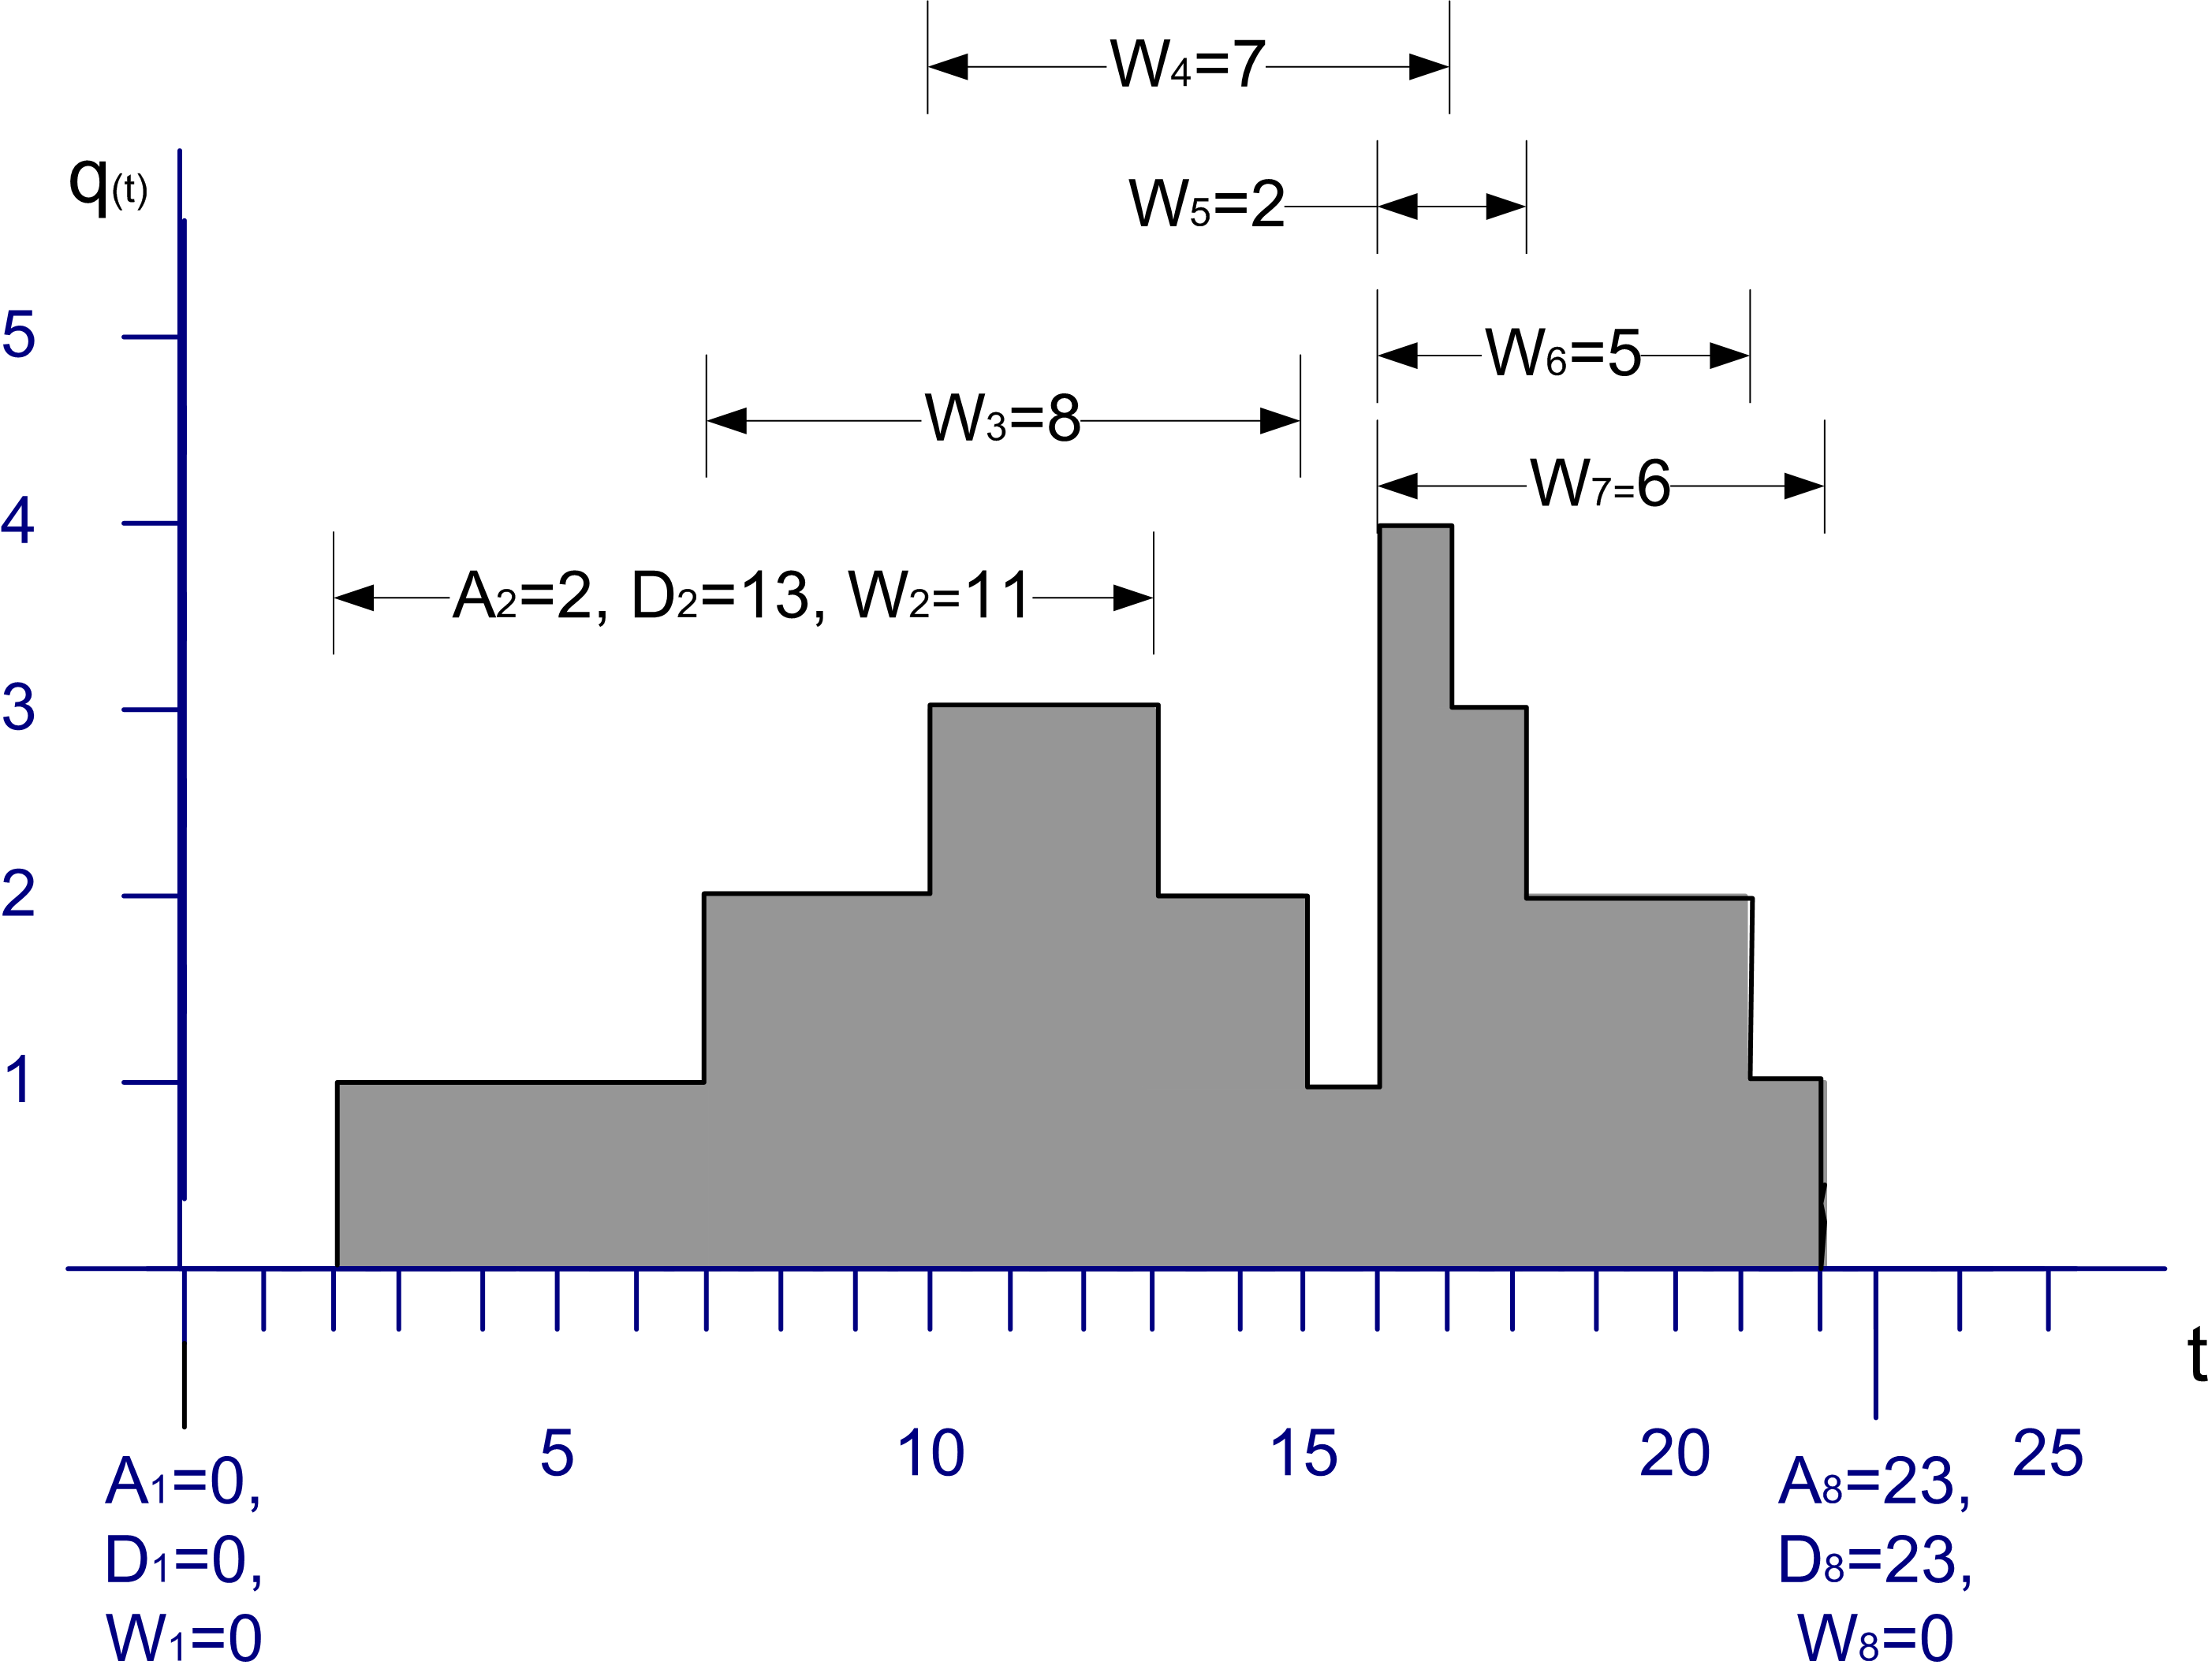
\includegraphics[width=0.8\linewidth,height=0.8\textheight]{./figures/ch7/ch7fig3} \caption{Sample Path for Tally and Time-Persistent Data}\label{fig:TallyTimePersistent}
\end{figure}

\begin{itemize}
\item
  Let \(A_i \; i = 1 \ldots n\) represent the time that the \(i^{th}\)
  customer enters the queue
\item
  Let \(D_i \; i = 1 \ldots n\) represent the time that the \(i^{th}\)
  customer exits the queue
\item
  Let \(W_i = D_i - A_i \; i = 1 \ldots n\) represent the time that the
  \(i^{th}\) customer spends in the queue
\end{itemize}

Thus, \(W_i \; i = 1 \ldots n\) represents the sequence of wait times for
the queue, each of which can be individually observed and tallied. This
is tally type data because the customer enters a state (the queued
state) at time \(A_i\) and exits the state at time \(D_i\). When the
customer exits the queue at time \(D_i\), the waiting time in queue,
\(W_i = D_i - A_i\) can be observed or tallied. \(W_i\) is only observable
at the instant \(D_i\). This makes \(W_i\) tally based data and, once
observed, its value never changes again with respect to time. Tally data
is most often associated with an entity that is moving through states
that are implied by the simulation model. An observation becomes
available each time the entity enters and subsequently exits the state.

With tally data it is natural to compute the sample average as a measure
of the central tendency of the data. Assume that you can observe \(n\)
customers entering and existing the queue, then the average waiting time
across the \(n\) customers is given by:

\[\bar{W}(n) = \dfrac{1}{n} \sum_{i=1}^{n} W_{i}\]

Many other statistical quantities, such as the minimum, maximum, and
sample variance, etc. can also be computed from these observations.
Unfortunately, within replication data is often (if not always)
correlated with respect to time. In other words, within replication
observations like, \(W_i \, i = 1 \ldots n\), are not statistically
independent. In fact, they are likely to also not be identically
distributed. Both of these issues will be discussed when the analysis of
infinite horizon or steady state simulation models is presented.

The other type of statistical variable encountered within a replication
is based on time-persistent observations. Let \(q(t), t_0 < t \leq t_n\)
be the number of customers in the queue at time \(t\). Note that
\(q(t) \in \lbrace 0,1,2,\ldots\rbrace\). As illustrated in
Figure \ref{fig:TallyTimePersistent}, \(q(t)\) is a function of time (a step
function in this particular case). That is, for a given (realized)
sample path, \(q(t)\) is a function that returns the number of customers
in the queue at time \(t\).

The mean value theorem of calculus for integrals states that given a
function, \(f(\cdot)\), continuous on an interval \([a, b]\), there exists a
constant, \(c\), such that

\[\int_a^b f(x) \mathrm{d}x = f(c)(b-a)\]

The value, \(f(c)\), is called the mean value of the function. A similar
function can be defined for \(q(t)\). In simulation, this function is
called the time-average:

\[\bar{L}_q(n) = \frac{1}{t_n - t_0} \int_{t_0}^{t_n} q(t) \mathrm{d}t\]

This function represents the average with respect to time of the given
state variable. This type of statistical variable is called
time-persistent because \(q(t)\) is a function of time (i.e.~it persists
over time).

In the particular case where \(q(t)\) represents the number of customers
in the queue, \(q(t)\) will take on constant values during intervals of
time corresponding to when the queue has a certain number of customers.
Let \(q(t)\) = \(q_k\) for \(t_{k-1} \leq t \leq t_k\) and define
\(v_k = t_k - t_{k-1}\) then the time-average number in queue can be
rewritten as follows:

\[
\begin{aligned}
\bar{L}_q(n) &= \frac{1}{t_n - t_0} \int_{t_0}^{t_n} q(t) \mathrm{d}t\\
 & = \frac{1}{t_n - t_0} \sum_{k=1}^{n} q_k (t_k - t_{k-1})\\
 & = \frac{\sum_{k=1}^{n} q_k v_k}{t_n - t_0} \\
 & = \frac{\sum_{k=1}^{n} q_k v_k}{\sum_{k=1}^{n} v_k}
\end{aligned}
\]

Note that \(q_k (t_k - t_{k-1})\) is the area under \(q(t)\) over the
interval \(t_{k-1} \leq t \leq t_k\) and

\[t_n - t_0 = \sum_{k=1}^{n} v_k = (t_1 - t_0) + (t_2 - t_1) + \cdots (t_{n-1} - t_{n-2}) + (t_n - t_{n-1})\]

is the total time over which the variable is observed. Thus, the time
average is simply the area under the curve divided by the amount of time
over which the curve is observed. From this equation, it should be noted
that each value of \(q_k\) is weighted by the length of time that the
variable has the value. This is why the time average is often called the
time-weighted average. If \(v_k = 1\), then the time average is the same
as the sample average.

With time-persistent data, you often want to estimate the percentage of
time that the variable takes on a particular value. Let \(T_i\) denote the
\emph{total} time during \(t_0 < t \leq t_n\) that the queue had \(q(t) = i\)
customers. To compute \(T_i\), you sum all the rectangles corresponding to
\(q(t) = i\), in the sample path. Because
\(q(t) \in \lbrace 0,1,2,\ldots\rbrace\) there are an infinite number of
possible value for \(q(t)\) in this example; however, within a finite
sample path you can only observe a finite number of the possible values.
The ratio of \(T_i\) to \(T = t_n - t_0\) can be used to estimate the
percentage of time the queue had \(i\) customers. That is, define
\(\hat{p}_i = T_i/T\) as an estimate of the proportion of time that the
queue had \(i\) customers during the interval of observation.

Let's look at an example. Consider Figure \ref{fig:TallyTimePersistent}, which shows the change in queue
length over a simulated period of 25 time units.

\begin{enumerate}
\def\labelenumi{\arabic{enumi}.}
\item
  Compute the time average number in queue over the interval of time
  from 0 to 25.
\item
  Compute the percentage of time that the queue had
  \(\lbrace 0, 1, 2, 3, 4\rbrace\) customers
\end{enumerate}

Since the queue length is a time-persistent variable, the time average queue length can be
computed as:

\[
\begin{aligned}
\bar{L}_q & = \frac{0(2-0) + 1(7-2) + 2(10-7) + 3(13-10) + 2(15-13) + 1(16-15)}{25}\\
 & + \frac{4(17-16) + 3(18-17) + 2(21-18) + 1(22-21) + 0(25-22)}{25} \\
 & = \frac{39}{25} = 1.56
\end{aligned}
\]

To estimate the percentage of time that the queue had
\(\lbrace 0, 1, 2, 3, 4\rbrace\) customers, the values of
\(v_k = t_k - t_{k-1}\) need to be summed for whenever
\(q(t) \in \lbrace 0, 1, 2, 3, 4 \rbrace\). This results in the following:

\[\hat{p}_0 = \dfrac{T_0}{T} = \dfrac{(2-0) + (25-22)}{25} = \dfrac{2 + 3}{25} = \dfrac{5}{25} = 0.2\]

\[\hat{p}_1 = \dfrac{T_1}{T} = \dfrac{(7-2) + (16-15) + (22-21)}{25} = \dfrac{5 + 1 + 1}{25} = \dfrac{7}{25} = 0.28\]

\[\hat{p}_2 = \dfrac{T_2}{T} = \dfrac{3 + 2 + 3)}{25} = \dfrac{8}{25} = 0.28\]

\[\hat{p}_3 = \dfrac{T_3}{T} = \dfrac{3 + 1}{25} = \dfrac{4}{25} = 0.16\]

\[\hat{p}_4 = \dfrac{T_4}{T} = \dfrac{1}{25} = \dfrac{1}{25} = 0.04\]

Notice that the sum of the \(\hat{p}_i\) adds to one. To compute the
average waiting time in the queue, use the supplied values for each
waiting time.

\[\bar{W}(8) = \frac{\sum_{i=1}^n W_i}{n} =\dfrac{0 + 11 + 8 + 7 + 2 + 5 + 6 + 0}{8} = \frac{39}{8} = 4.875\]

Notice that there were two customers, one at time 1.0 and another at
time 23.0 that had waiting times of zero. The state graph did not move
up or down at those times. Each unit increment in the queue length is
equivalent to a new customer entering (and staying in) the queue. On the
other hand, each unit decrement of the queue length signifies a
departure of a customer from the queue. If you assume a first-in,
first-out (FIFO) queue discipline, the waiting times of the six
customers that entered the queue (and had to wait) are shown in the
figure.

Now that we understand the type of data that occurs within a
replication, we need to develop an understanding for the types of
simulation situations that require specialized statistical analysis. The
next section introduces this important topic.

\hypertarget{simoa:simtypes}{%
\section{Types of Simulation With Respect To Output Analysis}\label{simoa:simtypes}}

When modeling a system, specific measurement goals for the simulation
responses are often required. The goals, coupled with how the system
operates, will determine how you execute and analyze the simulation
experiments. In planning the experimental analysis, it is useful to
think of simulations as consisting of two main categories related to the
period of time over which a decision needs to be made:

\begin{description}
\item[Finite horizon]
In a finite-horizon simulation, a well define ending time or ending
condition can be specified which clearly defines the end of the
simulation. Finite horizon simulations are often called
\emph{terminating} simulations, since there are clear terminating
conditions.
\item[Infinite horizon]
In an infinite horizon simulation, there is no well defined ending
time or condition. The planning period is over the life of the
system, which from a conceptual standpoint lasts forever. Infinite
horizon simulations are often called \emph{steady state} simulations
because in an infinite horizon simulation you are often interested
in the long-term or steady state behavior of the system.
\end{description}

For a finite horizon simulation, an event or condition associated with
the system is present which indicates the end of each simulation
replication. This event can be specified in advance or its time of
occurrence can be a random variable. If it is specified in advance, it
is often because you do not want information past that point in time
(e.g.~a 3 month planning horizon). It might be a random variable in the
case of the system stopping when a condition is met. For example, an
ending condition may be specified to stop the simulation when there are
no entities left to process. Finite horizon simulations are very common
since most planning processes are finite. A few example systems
involving a finite horizon include:

\begin{itemize}
\item
  Bank: bank doors open at 9am and close at 5pm
\item
  Military battle: simulate until force strength reaches a critical
  value
\item
  Filling a customer order: suppose a new contract is accepted to
  produce 100 products, you might simulate the production of the 100
  products to see the cost, delivery time, etc.
\end{itemize}

For a finite horizon simulation, each replication represents a sample
path of the model for one instance of the finite horizon. The length of
the replication corresponds to the finite horizon of interest. For
example, in modeling a bank that opens at 9 am and closes at 5 pm, the
length of the replication would be 8 hours.

In contrast to a finite horizon simulation, an infinite horizon
simulation has no natural ending point. Of course, when you actually
simulate an infinite horizon situation, a finite replication length must
be specified. Hopefully, the replication length will be long enough to
satisfy the goal of observing long run performance. Examples of infinite
horizon simulations include:

\begin{itemize}
\item
  A factory where you are interested in measuring the steady state
  throughput
\item
  A hospital emergency room which is open 24 hours a day, 7 days of
  week
\item
  A telecommunications system which is always operational
\end{itemize}

Infinite horizon simulations are often tied to systems that operate
continuously and for which the long-run or steady state behavior needs
to be estimated.

Because infinite horizon simulations often model situations where the
system is always operational, they often involve the modeling of
non-stationary processes. In such situations, care must be taken in
defining what is meant by long-run or steady state behavior. For
example, in an emergency room that is open 24 hours a day, 365 days per
year, the arrival pattern to such a system probably depends on time.
Thus, the output associated with the system is also non-stationary. The
concept of steady state implies that the system has been running so long
that the system's behavior (in the form of performance measures) no
longer depends on time; however, in the case of the emergency room since
the inputs depend on time so do the outputs. In such cases it is often
possible to find a period of time or cycle over which the non-stationary
behavior repeats. For example, the arrival pattern to the emergency room
may depend on the day of the week, such that every Monday has the same
characteristics, every Tuesday has the same characteristics, and so on
for each day of the week. Thus, on a weekly basis the non-stationary
behavior repeats. You can then define your performance measure of
interest based on the appropriate non-stationary cycle of the system.
For example, you can define Y as the expected waiting time of patients
\emph{per week}. This random variable may have performance that can be
described as long-term. In others, the long-run weekly performance of
the system may be stationary. This type of simulation has been termed
steady state cyclical parameter estimation within \citep{law2007simulation}.

Of the two types of simulations, finite horizon simulations are easier
to analyze. Luckily they are the more typical type of simulation found
in practice. In fact, when you think that you are faced with an infinite
horizon simulation, you should very carefully evaluate the goals of your
study to see if they can just as well be met with a finite planning
horizon. The analysis of both of these types of simulations will be
discussed in this chapter through examples.

\hypertarget{simoa:finhorizon}{%
\section{Analysis of Finite Horizon Simulations}\label{simoa:finhorizon}}

This section illustrates how tally-based and time-persistent statistics
are collected within a replication and how statistics are collected
across replications. Finite horizon simulations can be analyzed by
traditional statistical methodologies that assume a random sample, i.e.
independent and identically distributed random variables. A simulation
experiment is the collection of experimental design points (specific
input parameter values) over which the behavior of the model is
observed. For a particular design point, you may want to repeat the
execution of the simulation multiple times to form a sample at that
design point. To get a random sample, you execute the simulation
starting from the same initial conditions and ensure that the random
numbers used within each replication are independent. Each replication
must also be terminated by the same conditions. It is very important to
understand that independence is achieved across replications, i.e.~the
replications are independent. The data \emph{within} a replication may or may
not be independent.

The method of \emph{independent replications} is used to analyze finite
horizon simulations. Suppose that \(n\) replications of a simulation are
available where each replication is terminated by some event \(E\) and
begun with the same initial conditions. Let \(Y_{rj}\) be the \(j^{th}\)
observation on replication \(r\) for \(j = 1,2,\cdots,m_r\) where \(m_r\) is
the number of observations in the \(r^{th}\) replication, and
\(r = 1,2,\cdots,n\), and define the sample average for each replication
to be:

\[\bar{Y}_r = \frac{1}{m_r} \sum_{j=1}^{m_r} Y_{rj}\]

If the data are time-based then,

\[\bar{Y}_r = \frac{1}{T_E}  \int_0^{T_E} Y_r(t) \mathrm{d}t\]

\(\bar{Y}_r\) is the sample average based on the observation within the
\(r^{th}\) replication. It is a random variable that can be observed at
the end of each replication, therefore, \(\bar{Y}_r\) for
\(r = 1,2,\ldots,n\) forms a random sample. Thus, standard statistical
analysis of the random sample can be performed.

To make this concrete, suppose that you are examining a bank that opens
with no customers at 9 am and closes its doors at 5 pm to prevent
further customers from entering. Let, \(W_{rj} j = 1,\ldots,m_r\),
represents the sequence of waiting times for the customers that entered
the bank between 9 am and 5 pm on day (replication) \(r\) where \(m_r\) is
the number of customers who were served between 9 am and 5 pm on day
\(r\). For simplicity, ignore the customers who entered before 5 pm but
did not get served until after 5 pm. Let \(N_r (t)\) be the number of
customers in the system at time \(t\) for day (replication) \(r\). Suppose
that you are interested in the mean daily customer waiting time and the
mean number of customers in the bank on any given 9 am to 5 pm day, i.e.
you are interested in \(E[W_r]\) and \(E[N_r]\) for any given day. At the
end of each replication, the following can be computed:

\[\bar{W}_r = \frac{1}{m_r} \sum_{j=1}^{m_r} W_{rj}\]

\[\bar{N}_r = \dfrac{1}{8}\int_0^8 N_r(t)\ \mathrm{d}t\]

At the end of all replications, random samples: \(\bar{W}_r\) and
\(\bar{N}_r\) are available from which sample averages, standard
deviations, confidence intervals, etc. can be computed. Both of these
samples are based on observations of within replication data.

Both \(\bar{W_r}\) and \(\bar{N_r}\) for \(r = 1,2,\ldots,n\) are averages of many observations
within the replication. Sometimes, there may only be one observation
based on the entire replication. For example, suppose that you are
interested in the probability that someone is still in the bank when the
doors close at 5 pm, i.e.~you are interested in
\(\theta = Pr\{N(t = 5 pm) > 0\}\). In order to estimate this probability,
an indicator variable can be defined within the simulation and observed
each time the condition was met or not. For this situation, an indicator
variable,\(I_r\), for each replication can be defined as follows:

\[
I_r =
   \begin{cases}
     1 & N(t = 5 pm) > 0\\
     0 & N(t = 5 pm) \leq 0 \\
  \end{cases}
\]

Therefore, at the end of the replication, the simulation must tabulate
whether or not there are customers in the bank and record the value of
this indicator variable. Since this happens only once per replication, a
random sample of the \(I_r\) for \(r = 1,2,\ldots,n\) will be available after all
replications have been executed. We can use
the observations of the indicator variable to estimate the desired
probability.

Since the analysis of the system will be based on a random sample, the
key design criteria for the experiment will be the required number of
replications. In other words, you need to determine the sample size.

Because confidence intervals may form the basis for decision making, you
can use the confidence interval half-width in determining the sample
size. For example, in estimating \(E[W_r]\) for the bank example, you
might want to be 95\% confident that you have estimated the true waiting
time to within \(\pm 2\) minutes.

There are three related methods that are commonly used for determining
the sample size for this situation:

\begin{itemize}
\item
  an iterative method based on the t-distribution,
\item
  an approximate method based on the normal distribution, and
\item
  the half-width ratio method
\end{itemize}

Each of these methods assumes that the observations in the sample are
independent and identically distributed from a normal distribution. In
addition, the methods also assume that the pilot replications are
representative of the population under study. When the data are not
normally distributed, you must rely on the central limit theorem to get
approximate results. The assumption of normality is typically justified
when across replication statistics are based on within replication
averages.

Since the first two methods have previously been presented, this chapter will discuss the half-width ratio method because it is often seen in practice.

\hypertarget{simoa:finhorizon:samplesize}{%
\subsection{Determining the Number of Replications}\label{simoa:finhorizon:samplesize}}

If you make a pilot run of \(n_0\) replications you can use the half-width from the pilot run
to determine how many replications you need to have to be close to a
desired half-width bound in the full experiment. This is called the
\emph{half-width ratio method}.

Let \(h_0\) be the initial value for the half-width from the pilot run of
\(n_0\) replications.

\begin{equation}
h_0 = t_{\alpha/2, n_0 - 1} \dfrac{s_0}{\sqrt{n_0}}
\label{eq:hNot}
\end{equation}

Solving for \(n_0\) yields:

\begin{equation}
n_0 = t_{\alpha/2, n_0 -1}^{2} \dfrac{s_{0}^{2}}{h_{0}^{2}}
(\#eq:n_0)
\end{equation}

Similarly for any \(n\), we have:

\begin{equation}
n = t_{\alpha/2, n-1}^{2} \dfrac{s^{2}}{h^{2}}
\label{eq:n}
\end{equation}

Taking the ratio of \(n_0\) to \(n\) (equations @ref(eq:n\_0) and \eqref{eq:n}) and assuming
that \(t_{\alpha/2, n-1}\) is approximately equal to
\(t_{\alpha/2, n_0 - 1}\) and \(s^2\) is approximately equal to \(s_0^2\),
yields,

\begin{equation}
n \cong n_0 \dfrac{h_0^2}{h^2} = n_0 \left(\frac{h_0}{h}\right)^2
\label{eq:hwratio}
\end{equation}

Equation (\eqref{eq:hwratio}) is the half-width ratio equation.

In the case of an indicator variable such as, \(I_r\), which was suggested
for use in estimating the probability that there are customers in the
bank after 5 pm, the sampled observations are clearly not normally
distributed. In this case, since you are estimating a proportion, you
can use the sample size determination techniques for estimating
proportions previously described.

Now, let's look at an example. Suppose a pilot run of a
simulation model estimated that the average waiting time for a customer
during the day was 11.485 minutes based on an initial sample size of 15
replications with a 95\% confidence interval half-width of 1.04. Using
the three sample size determination techniques, recommend a sample size
to be 95\% confident that you are within \(\pm 0.10\) of the true mean
waiting time in the queue.

First we will do the half-width ratio method. We have that \(h_0 = 1.04\),
\(n_0 = 15\), and \(h = 0.1\), thus:

\[n \cong n_0 \left(\frac{h_0}{h}\right)^2 = 15 \left(\frac{1.04}{0.1}\right)^2 = 1622.4 \cong 1623\]

To estimate a sample size based on the normal approximation method, we
need to have the estimate of the initial sample standard deviation.
Unfortunately, this is not directly reported, but it can be computed
using Equation (\eqref{eq:hNot}). Rearranging Equation (\eqref{eq:hNot})
to solve for \(s_0\), yields:

\[s_0 = \dfrac{h_0\sqrt{n_0}}{t_{\alpha/2, n_0 - 1}}\]

Since we have a 95\% confidence interval with \(n_0 = 15\), we have that
\(t_{0.025, 14} = 2.145\), which yields,

\[s_0 = \dfrac{h_0\sqrt{n_0}}{t_{\alpha/2, n_0 - 1}} = \dfrac{1.04\sqrt{15}}{2.145} =  1.87781\]

Now, we can use the normal approximation method. By using \(h\) as the
desired bound \(E\) and \(z_{0.025} = 1.96\), we have,

\[n \geq \biggl(\dfrac{z_{\alpha/2} s}{E}\biggr)^2 = \biggl(\dfrac{1.96 \times 1.87781}{0.1}\biggr)^2 = 1354.54 \approx 1355\]

The final method is to use the iterative method based on the following equation:

\[h = t_{\alpha/2, n-1} \dfrac{s}{\sqrt{n}} \leq E\]

This can be accomplished easily within a spreadsheet yielding \(n=1349\).

\begin{figure}
\centering
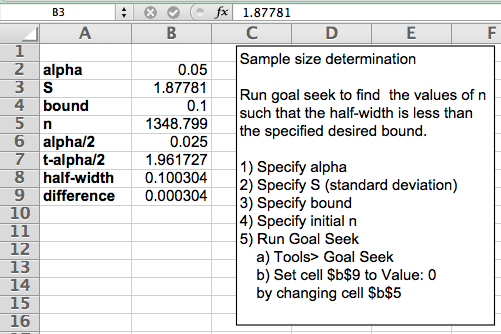
\includegraphics{./figures/ch7/ch7SampleSizeViaGoalSeek.png}
\caption{\label{fig:SampleSizeViaGoalSeek}Iterative Method for Sample Size via Goal Seek}
\end{figure}

The three methods resulted in following recommendations:

\begin{itemize}
\item
  an iterative method based on the t-distribution, n = 1349
\item
  an approximate method based on the normal distribution, n = 1355
\item
  the half-width ratio method, n = 1623
\end{itemize}

As noted in the discussion, the half-width ratio method recommended the
largest number of replications.

\hypertarget{simoa:finhorizonex}{%
\section{Finite Horizon Example}\label{simoa:finhorizonex}}

This section presents a fictitious system involving the production of rings. The example illustrates how to collect tally based
statistics, time based statistics, and statistics that can only be
collected at the end of a replication. The analysis of a finite horizon
simulation will be illustrated. In addition, the
system also represents another example of how to use the station package.

Every morning the sales force at LOTR Makers, Inc.~makes a number of confirmation
calls to customers who have previously been visited by the sales force.
They have tracked the success rate of their confirmation calls over time
and have determined that the chance of success varies from day to day.
They have modeled the probability of success for a given day as a beta
random variable with parameters \(\alpha_1 = 5\) and \(\alpha_2 = 1.5\) so
that the mean success rate is about 77\%. They always make 100 calls
every morning. Each sales call will or will not result in an order for a
pair of magical rings for that day. Thus, the number of pairs of rings
to produce every day is a binomial random variable, with \(p\) determined
by the success rate for the day and \(n = 100\) representing the total
number of calls made. Note that \(p\) is random in this modeling.

The sales force is large enough and the time to make the confirmation
calls small enough so as to be able to complete all the calls before
releasing a production run for the day. In essence, ring production does
not start until all the orders have been confirmed, but the actual
number of ring pairs produced every day is unknown until the sales call
confirmation process is completed. The time to make the calls is
negligible when compared to the overall production time.

Besides being magical, one ring is smaller than the other ring so that
the smaller ring must fit snuggly inside the larger ring. The pair of
rings is produced by a master ring maker and takes uniformly between 5
to 15 minutes. The rings are then scrutinized by an inspector with the
time (in minutes) being distributed according to a triangular
distribution with parameters (2, 4, 7) for the minimum, the mode, and
the maximum. The inspection determines whether the smaller ring is too
big or too small when fit inside the bigger outer ring. The inside
diameter of the bigger ring, \(D_b\), is normally distributed with a mean
of 1.5 cm and a standard deviation of 0.002. The outside diameter of the
smaller ring, \(D_s\), is normally distributed with a mean of 1.49 and a
standard deviation of 0.005. If \(D_s > D_b\), then the smaller ring will
not fit in the bigger ring; however, if \(D_b - D_s > tol\), then the
rings are considered too loose. The tolerance is currently set at 0.02
cm.

If there are no problems with the rings, the rings are sent to a packer
for custom packaging for shipment. A time study of the packaging time
indicates that it is distributed according to a log-normal distribution
with a mean of 7 minutes and a standard deviation of 1 minute. If the
inspection shows that there is a problem with the pair of rings they are
sent to a rework craftsman. The minimum time that it takes to rework the
pair of rings has been determined to be 5 minutes plus some random time
that is distributed according to a Weibull distribution with a scale
parameter of 15 and a shape parameter of 5. After the rework is
completed, the pair of rings is sent to packaging.

Currently, the company runs two shifts of 480 minutes each. Time after
the end of the second shift is considered overtime. Management is
interested in investigating the following:

\begin{itemize}
\item
  The daily production time.
\item
  The probability of overtime.
\item
  The average number of pairs of rings in both the ring making process
  and the ring inspection process.
\item
  The average time that it takes for a pair of rings to go through
  both the ring making process and the ring inspection process. In
  addition, a 95\% confidence interval for the mean time to complete
  these processes to within \(\pm\) 20 minutes is desired.
\end{itemize}

\hypertarget{conceptualizing-the-model}{%
\subsection{Conceptualizing the Model}\label{conceptualizing-the-model}}

Now let's proceed with the modeling of this situation. We start with answering the basic model
building questions.

\emph{What is the system? What information is known by the system?}

The system is the LOTR Makers, Inc.~sales calls and ring production
processes. The system starts every day with the initiation of sales
calls and ends when the last pair of rings produced for the day is
shipped. The system knows the following:

\begin{itemize}
\item
  Sales call success probability distribution:
  \(p \sim beta(\alpha_1 = 5,\alpha_2 = 1.5)\)
\item
  Number of calls to be made every morning: \(n = 100\)
\item
  Distribution of time to make the pair of rings: \(U(5,15)\)
\item
  Distributions associated with the big and small ring diameters:
  N(\(\mu\) = 1.5, \(\sigma\) = 0.002) and N(\(\mu\) = 1.49, \(\sigma\) =
  0.005), respectively
\item
  Distribution of ring-inspection time: triangular(2,4,7)
\item
  Distribution of packaging time: lognormal(\(\mu_{l}\) = 7,\(\sigma_{l}\)
  = 1)
\item
  Distribution of rework time, 5 + Weibull(scale =15, shape =3)
\item
  Length of a shift: 480 minutes
\end{itemize}

\emph{What are the entities? What information must be recorded for each entity?}

Possible entities are the sales calls and the production job (pair of
rings) for every successful sales call. For every pair of rings, the
diameters must be known.

\emph{What are the resources that are used by the entities?}

The sales calls do not use any resources. The production job uses a
master craftsman, an inspector, and a packager. It might also use a
rework craftsman.

\emph{What are the activities? What are the processes? What are the events associated with the processes and activities? Write out or draw sketches of the process.}

There are two processes: sales order and production. An outline of the
sales order process should look like this:

\begin{enumerate}
\def\labelenumi{\arabic{enumi}.}
\item
  Start the day.
\item
  Determine the likelihood of calls being successful.
\item
  Make the calls.
\item
  Determine the total number of successful calls.
\item
  Start the production jobs.
\end{enumerate}

Notice that the sales order process takes zero time and that it occurs
at the beginning of each day. Thus, there appears to be an event that
occurs at time 0.0, that determines the number of production jobs and
sends them to production. This type of situation is best modeled using
the initialize() method to make the orders to be placed into production.
From the problem statement, the number of production jobs is a binomial
random variable with \(n= 100\) and
\(p \sim BETA(\alpha_1 = 5,\alpha_2 = 1.5)\).

The following listing shows the constructor for this model and the
initialize() method.

\begin{Shaded}
\begin{Highlighting}[]
\KeywordTok{public} \FunctionTok{LOTR}\OperatorTok{(}\NormalTok{ModelElement parent}\OperatorTok{,} \BuiltInTok{String}\NormalTok{ name}\OperatorTok{)} \OperatorTok{\{}
    \KeywordTok{super}\OperatorTok{(}\NormalTok{parent}\OperatorTok{,}\NormalTok{ name}\OperatorTok{);}
\NormalTok{    mySalesCallProb }\OperatorTok{=} \KeywordTok{new} \FunctionTok{RandomVariable}\OperatorTok{(}\KeywordTok{this}\OperatorTok{,} \KeywordTok{new} \FunctionTok{BetaRV}\OperatorTok{(}\FloatTok{5.0}\OperatorTok{,} \FloatTok{1.5}\OperatorTok{));}
\NormalTok{    myMakeRingTimeRV }\OperatorTok{=} \KeywordTok{new} \FunctionTok{RandomVariable}\OperatorTok{(}\KeywordTok{this}\OperatorTok{,} \KeywordTok{new} \FunctionTok{UniformRV}\OperatorTok{(}\DecValTok{5}\OperatorTok{,} \DecValTok{15}\OperatorTok{));}
\NormalTok{    mySmallRingODRV }\OperatorTok{=} \KeywordTok{new} \FunctionTok{RandomVariable}\OperatorTok{(}\KeywordTok{this}\OperatorTok{,} \KeywordTok{new} \FunctionTok{NormalRV}\OperatorTok{(}\FloatTok{1.49}\OperatorTok{,} \FloatTok{0.005} \OperatorTok{*} \FloatTok{0.005}\OperatorTok{));}
\NormalTok{    myBigRingIDRV }\OperatorTok{=} \KeywordTok{new} \FunctionTok{RandomVariable}\OperatorTok{(}\KeywordTok{this}\OperatorTok{,} \KeywordTok{new} \FunctionTok{NormalRV}\OperatorTok{(}\FloatTok{1.5}\OperatorTok{,} \FloatTok{0.002} \OperatorTok{*} \FloatTok{0.002}\OperatorTok{));}
\NormalTok{    myInspectTimeRV }\OperatorTok{=} \KeywordTok{new} \FunctionTok{RandomVariable}\OperatorTok{(}\KeywordTok{this}\OperatorTok{,} \KeywordTok{new} \FunctionTok{TriangularRV}\OperatorTok{(}\DecValTok{2}\OperatorTok{,} \DecValTok{4}\OperatorTok{,} \DecValTok{7}\OperatorTok{));}
\NormalTok{    myPackingTimeRV }\OperatorTok{=} \KeywordTok{new} \FunctionTok{RandomVariable}\OperatorTok{(}\KeywordTok{this}\OperatorTok{,} \KeywordTok{new} \FunctionTok{LognormalRV}\OperatorTok{(}\DecValTok{7}\OperatorTok{,} \DecValTok{1}\OperatorTok{));}
\NormalTok{    myReworkTimeRV }\OperatorTok{=} \KeywordTok{new} \FunctionTok{RandomVariable}\OperatorTok{(}\KeywordTok{this}\OperatorTok{,} \KeywordTok{new} \FunctionTok{ShiftedRV}\OperatorTok{(}\FloatTok{5.0}\OperatorTok{,} \KeywordTok{new} \FunctionTok{WeibullRV}\OperatorTok{(}\DecValTok{3}\OperatorTok{,} \DecValTok{15}\OperatorTok{)));}
\NormalTok{    myRingMakingStation }\OperatorTok{=} \KeywordTok{new} \FunctionTok{SingleQueueStation}\OperatorTok{(}\KeywordTok{this}\OperatorTok{,}\NormalTok{ myMakeRingTimeRV}\OperatorTok{,}
            \StringTok{"RingMakingStation"}\OperatorTok{);}
\NormalTok{    myInspectionStation }\OperatorTok{=} \KeywordTok{new} \FunctionTok{SingleQueueStation}\OperatorTok{(}\KeywordTok{this}\OperatorTok{,}\NormalTok{ myInspectTimeRV}\OperatorTok{,}
            \StringTok{"InspectStation"}\OperatorTok{);}
\NormalTok{    myReworkStation }\OperatorTok{=} \KeywordTok{new} \FunctionTok{SingleQueueStation}\OperatorTok{(}\KeywordTok{this}\OperatorTok{,}\NormalTok{ myReworkTimeRV}\OperatorTok{,}
            \StringTok{"ReworkStation"}\OperatorTok{);}
\NormalTok{    myPackagingStation }\OperatorTok{=} \KeywordTok{new} \FunctionTok{SingleQueueStation}\OperatorTok{(}\KeywordTok{this}\OperatorTok{,}\NormalTok{ myPackingTimeRV}\OperatorTok{,}
            \StringTok{"PackingStation"}\OperatorTok{);}
\NormalTok{    myRingMakingStation}\OperatorTok{.}\FunctionTok{setNextReceiver}\OperatorTok{(}\NormalTok{myInspectionStation}\OperatorTok{);}
\NormalTok{    myInspectionStation}\OperatorTok{.}\FunctionTok{setNextReceiver}\OperatorTok{(}\KeywordTok{new} \FunctionTok{AfterInspection}\OperatorTok{());}
\NormalTok{    myReworkStation}\OperatorTok{.}\FunctionTok{setNextReceiver}\OperatorTok{(}\NormalTok{myPackagingStation}\OperatorTok{);}
\NormalTok{    myPackagingStation}\OperatorTok{.}\FunctionTok{setNextReceiver}\OperatorTok{(}\KeywordTok{new} \FunctionTok{Dispose}\OperatorTok{());}
\NormalTok{    mySystemTime }\OperatorTok{=} \KeywordTok{new} \FunctionTok{ResponseVariable}\OperatorTok{(}\KeywordTok{this}\OperatorTok{,} \StringTok{"System Time"}\OperatorTok{);}
\NormalTok{    myNumInSystem }\OperatorTok{=} \KeywordTok{new} \FunctionTok{TimeWeighted}\OperatorTok{(}\KeywordTok{this}\OperatorTok{,} \StringTok{"Num in System"}\OperatorTok{);}
\NormalTok{    myNumCompleted }\OperatorTok{=} \KeywordTok{new} \FunctionTok{Counter}\OperatorTok{(}\KeywordTok{this}\OperatorTok{,} \StringTok{"Num Completed"}\OperatorTok{);}
\NormalTok{    myProbTooBig }\OperatorTok{=} \KeywordTok{new} \FunctionTok{ResponseVariable}\OperatorTok{(}\KeywordTok{this}\OperatorTok{,} \StringTok{"Prob too Big"}\OperatorTok{);}
\NormalTok{    myProbTooSmall }\OperatorTok{=} \KeywordTok{new} \FunctionTok{ResponseVariable}\OperatorTok{(}\KeywordTok{this}\OperatorTok{,} \StringTok{"Prob too Small"}\OperatorTok{);}
\NormalTok{    myProbOT }\OperatorTok{=} \KeywordTok{new} \FunctionTok{ResponseVariable}\OperatorTok{(}\KeywordTok{this}\OperatorTok{,} \StringTok{"Prob of Over Time"}\OperatorTok{);}
\NormalTok{    myEndTime }\OperatorTok{=} \KeywordTok{new} \FunctionTok{ResponseVariable}\OperatorTok{(}\KeywordTok{this}\OperatorTok{,} \StringTok{"Time to Make Orders"}\OperatorTok{);}
\NormalTok{    myNumInRMandInspection }\OperatorTok{=} \KeywordTok{new} \FunctionTok{TimeWeighted}\OperatorTok{(}\KeywordTok{this}\OperatorTok{,} \StringTok{"Num in RM and Inspection"}\OperatorTok{);}
\NormalTok{    myTimeInRMandInspection }\OperatorTok{=} \KeywordTok{new} \FunctionTok{ResponseVariable}\OperatorTok{(}\KeywordTok{this}\OperatorTok{,} \StringTok{"Time in RM and Inspection"}\OperatorTok{);}
\OperatorTok{\}}

\AttributeTok{@Override}
\KeywordTok{protected} \DataTypeTok{void} \FunctionTok{initialize}\OperatorTok{()} \OperatorTok{\{}
    \KeywordTok{super}\OperatorTok{.}\FunctionTok{initialize}\OperatorTok{();}
    \DataTypeTok{double}\NormalTok{ p }\OperatorTok{=}\NormalTok{ mySalesCallProb}\OperatorTok{.}\FunctionTok{getValue}\OperatorTok{();}
    \DataTypeTok{int}\NormalTok{ n }\OperatorTok{=}\NormalTok{ JSLRandom}\OperatorTok{.}\FunctionTok{rBinomial}\OperatorTok{(}\NormalTok{p}\OperatorTok{,}\NormalTok{ myNumDailyCalls}\OperatorTok{);}
    \ControlFlowTok{for} \OperatorTok{(}\DataTypeTok{int}\NormalTok{ i }\OperatorTok{=} \DecValTok{0}\OperatorTok{;}\NormalTok{ i }\OperatorTok{\textless{}}\NormalTok{ n}\OperatorTok{;}\NormalTok{ i}\OperatorTok{++)} \OperatorTok{\{}
\NormalTok{        myRingMakingStation}\OperatorTok{.}\FunctionTok{receive}\OperatorTok{(}\KeywordTok{new} \FunctionTok{RingOrder}\OperatorTok{());}
\NormalTok{        myNumInSystem}\OperatorTok{.}\FunctionTok{increment}\OperatorTok{();}
\NormalTok{        myNumInRMandInspection}\OperatorTok{.}\FunctionTok{increment}\OperatorTok{();}
    \OperatorTok{\}}
\OperatorTok{\}}
\end{Highlighting}
\end{Shaded}

The constructor makes the random variables that
model the number of successful calls and the probability that a call is
successful. Then, the initialize() method, which is automatically called
at the beginning of a replication (essentially at time 0.0), uses the
random variables to first determine the probability of a successful call
and then determines the number of successful calls.
Finally, a for-loop is used to make the orders (new RingOrder()) and
send them into production at the ring making station. Also,
the number of orders in the system and the number of orders at the ring
making and inspection stations is incremented.

The following code listing illustrates the modeling of the orders within
the system.

\begin{Shaded}
\begin{Highlighting}[]
\KeywordTok{private} \KeywordTok{class}\NormalTok{ RingOrder }\KeywordTok{extends}\NormalTok{ QObject }\OperatorTok{\{}

    \KeywordTok{private} \DataTypeTok{double}\NormalTok{ myBigRingID}\OperatorTok{;}
    \KeywordTok{private} \DataTypeTok{double}\NormalTok{ mySmallRingOuterD}\OperatorTok{;}
    \KeywordTok{private} \DataTypeTok{double}\NormalTok{ myGap}\OperatorTok{;}
    \KeywordTok{private} \DataTypeTok{boolean}\NormalTok{ myNeedsReworkFlag }\OperatorTok{=} \KeywordTok{false}\OperatorTok{;}
    \KeywordTok{private} \DataTypeTok{boolean}\NormalTok{ myTooBigFlag }\OperatorTok{=} \KeywordTok{false}\OperatorTok{;}
    \KeywordTok{private} \DataTypeTok{boolean}\NormalTok{ myTooSmallFlag }\OperatorTok{=} \KeywordTok{false}\OperatorTok{;}

    \KeywordTok{public} \FunctionTok{RingOrder}\OperatorTok{()} \OperatorTok{\{}
        \KeywordTok{this}\OperatorTok{(}\FunctionTok{getTime}\OperatorTok{(),} \KeywordTok{null}\OperatorTok{);}
    \OperatorTok{\}}

    \KeywordTok{public} \FunctionTok{RingOrder}\OperatorTok{(}\DataTypeTok{double}\NormalTok{ creationTime}\OperatorTok{,} \BuiltInTok{String}\NormalTok{ name}\OperatorTok{)} \OperatorTok{\{}
        \KeywordTok{super}\OperatorTok{(}\NormalTok{creationTime}\OperatorTok{,}\NormalTok{ name}\OperatorTok{);}
\NormalTok{        myBigRingID }\OperatorTok{=}\NormalTok{ myBigRingIDRV}\OperatorTok{.}\FunctionTok{getValue}\OperatorTok{();}
\NormalTok{        mySmallRingOuterD }\OperatorTok{=}\NormalTok{ mySmallRingODRV}\OperatorTok{.}\FunctionTok{getValue}\OperatorTok{();}
\NormalTok{        myGap }\OperatorTok{=}\NormalTok{ myBigRingID }\OperatorTok{{-}}\NormalTok{ mySmallRingOuterD}\OperatorTok{;}
        \ControlFlowTok{if} \OperatorTok{(}\NormalTok{mySmallRingOuterD }\OperatorTok{\textgreater{}}\NormalTok{ myBigRingID}\OperatorTok{)} \OperatorTok{\{}
\NormalTok{            myTooBigFlag }\OperatorTok{=} \KeywordTok{true}\OperatorTok{;}
\NormalTok{            myNeedsReworkFlag }\OperatorTok{=} \KeywordTok{true}\OperatorTok{;}
        \OperatorTok{\}} \ControlFlowTok{else} \ControlFlowTok{if} \OperatorTok{(}\NormalTok{myGap }\OperatorTok{\textgreater{}}\NormalTok{ myRingTol}\OperatorTok{)} \OperatorTok{\{}
\NormalTok{            myTooSmallFlag }\OperatorTok{=} \KeywordTok{true}\OperatorTok{;}
\NormalTok{            myNeedsReworkFlag }\OperatorTok{=} \KeywordTok{true}\OperatorTok{;}
        \OperatorTok{\}}
    \OperatorTok{\}}

\OperatorTok{\}}
\end{Highlighting}
\end{Shaded}

A RingOrder represents an order for a pair of rings.
RingOrder is an inner class of LOTR. This was done so that the RingOrder
has easy access to the random variables defined within the LOTR class.
The outer ring's inner diameter and the inner ring's outer diameter are
modeled using attributes for the order. The values for these attributes
are set using the random variables that were defined as instance
variables of the LOTR class and instantiated within the LOTR class's
constructor. The size of the gap and whether or not the ring needs
rework is also computed. The condition of the ring in terms of whether
the gap is too big or too small is specified. Since the RingOrder class
extends the QObject class it has the ability to be held by instances of
the Queue class. Once the order for the rings is made it is passed into
production.

An outline of the production process should be something like this:

\begin{enumerate}
\def\labelenumi{\arabic{enumi}.}
\item
  Make the rings (determine sizes).
\item
  Inspect the rings.
\item
  If rings do not pass inspection, perform rework
\item
  Package rings and ship.
\end{enumerate}

Notice that in the production of the rings there are a number of
activities that take place during which various resources are used. This
situation is very similar to the Tie-Dye T-Shirt example in that the
rings move from ring making to inspection (possibly rework) and finally
to packaging. Each of these areas can be modeled using the
SingleQueueStation class. The
events associated with this situation include arrival to ring making,
departure from ring making, arrival to inspection, departure from
inspection, arrvial to rework, departure from rework, arrival to
packaging and departure from packaging. Since the departure from an
upstream station also represents an arrival to the downstream station,
the number of events needed to model this situation can be consolidated.
As mentioned, the SingleQueueStation can be used to model this situation
by connecting the stations together. The construction of the stations
and their connection is illustrated in the constructor for the LOTR system. Notice that the setNextReceiver() methods
are used to connect the ring making station to the inspection station
and to have the rework station send work to the packaging station.

One conceptually challenging aspect of this model is the fact that the
rings will probabilistically go to the rework station or the packaging
station. To model this situation, an inner class called AfterInspection
was designed that implements the ReceiveQObjectIfc interface. An
instance of this class is provided as the receiver for the inspection
station. Thus, after the inspection station is done,
the order for the ring (in the form of a QObject) will be sent to this
logic.

In the following listing, lines 4 and 5 finish out the collection of
the number of orders in the ring making and inspection stations and the
collection of the time spent within those stations. Then, starting in
line 6, the order is checked if it needs rework and if so, the rework
station is told to receive it; otherwise, the packaging station is told
to receive it.

\begin{Shaded}
\begin{Highlighting}[]
\KeywordTok{protected} \KeywordTok{class}\NormalTok{ AfterInspection }\KeywordTok{implements}\NormalTok{ ReceiveQObjectIfc }\OperatorTok{\{}
    \AttributeTok{@Override}
    \KeywordTok{public} \DataTypeTok{void} \FunctionTok{receive}\OperatorTok{(}\NormalTok{QObject qObj}\OperatorTok{)} \OperatorTok{\{}
\NormalTok{        myNumInRMandInspection}\OperatorTok{.}\FunctionTok{decrement}\OperatorTok{();}
\NormalTok{        myTimeInRMandInspection}\OperatorTok{.}\FunctionTok{setValue}\OperatorTok{(}\FunctionTok{getTime}\OperatorTok{()} \OperatorTok{{-}}\NormalTok{ qObj}\OperatorTok{.}\FunctionTok{getCreateTime}\OperatorTok{());}
\NormalTok{        RingOrder order }\OperatorTok{=} \OperatorTok{(}\NormalTok{RingOrder}\OperatorTok{)}\NormalTok{ qObj}\OperatorTok{;}
        \ControlFlowTok{if} \OperatorTok{(}\NormalTok{order}\OperatorTok{.}\FunctionTok{myNeedsReworkFlag}\OperatorTok{)} \OperatorTok{\{}
\NormalTok{            myReworkStation}\OperatorTok{.}\FunctionTok{receive}\OperatorTok{(}\NormalTok{order}\OperatorTok{);}
        \OperatorTok{\}} \ControlFlowTok{else} \OperatorTok{\{}
\NormalTok{            myPackagingStation}\OperatorTok{.}\FunctionTok{receive}\OperatorTok{(}\NormalTok{order}\OperatorTok{);}
        \OperatorTok{\}}
    \OperatorTok{\}}
\OperatorTok{\}}

\KeywordTok{protected} \KeywordTok{class}\NormalTok{ Dispose }\KeywordTok{implements}\NormalTok{ ReceiveQObjectIfc }\OperatorTok{\{}
    \AttributeTok{@Override}
    \KeywordTok{public} \DataTypeTok{void} \FunctionTok{receive}\OperatorTok{(}\NormalTok{QObject qObj}\OperatorTok{)} \OperatorTok{\{}
        \CommentTok{// collect final statistics}
\NormalTok{        RingOrder order }\OperatorTok{=} \OperatorTok{(}\NormalTok{RingOrder}\OperatorTok{)}\NormalTok{ qObj}\OperatorTok{;}
\NormalTok{        myNumInSystem}\OperatorTok{.}\FunctionTok{decrement}\OperatorTok{();}
\NormalTok{        mySystemTime}\OperatorTok{.}\FunctionTok{setValue}\OperatorTok{(}\FunctionTok{getTime}\OperatorTok{()} \OperatorTok{{-}}\NormalTok{ order}\OperatorTok{.}\FunctionTok{getCreateTime}\OperatorTok{());}
\NormalTok{        myNumCompleted}\OperatorTok{.}\FunctionTok{increment}\OperatorTok{();}
\NormalTok{        myProbTooBig}\OperatorTok{.}\FunctionTok{setValue}\OperatorTok{(}\NormalTok{order}\OperatorTok{.}\FunctionTok{myTooBigFlag}\OperatorTok{);}
\NormalTok{        myProbTooSmall}\OperatorTok{.}\FunctionTok{setValue}\OperatorTok{(}\NormalTok{order}\OperatorTok{.}\FunctionTok{myTooSmallFlag}\OperatorTok{);}
    \OperatorTok{\}}
\OperatorTok{\}}

\AttributeTok{@Override}
\KeywordTok{protected} \DataTypeTok{void} \FunctionTok{replicationEnded}\OperatorTok{()} \OperatorTok{\{}
    \KeywordTok{super}\OperatorTok{.}\FunctionTok{replicationEnded}\OperatorTok{();}
\NormalTok{    myProbOT}\OperatorTok{.}\FunctionTok{setValue}\OperatorTok{(}\FunctionTok{getTime}\OperatorTok{()} \OperatorTok{\textgreater{}}\NormalTok{ myOTLimit}\OperatorTok{);}
\NormalTok{    myEndTime}\OperatorTok{.}\FunctionTok{setValue}\OperatorTok{(}\FunctionTok{getTime}\OperatorTok{());}
\OperatorTok{\}}
\end{Highlighting}
\end{Shaded}

Similar to previous examples, the Dispose inner class collects
statistics at the system level and on the orders as they depart the
system. Besides the collection of the number orders in the ring making
and inspection stations, management also desired the collection of the
probability of over time and the time that the production run will be
completed. The collection of the chance of over time depends on when all
of the production are completed. The problem statement requests the
estimation of the probability of overtime work. The sales order process
determines the number of rings to produce. The production process
continues until there are no more rings to produce for that day. The
number of rings to produce is a binomial random variable as determined
by the sales order confirmation process. Thus, there is no clear run
length for this simulation.

In the JSL, a replication of a simulation can end based on three
situations:

\begin{enumerate}
\def\labelenumi{\arabic{enumi}.}
\item
  A scheduled run length
\item
  A terminating condition is met
\item
  No more events to process
\end{enumerate}

Because the production for the day stops when all the rings are
produced, the third situation applies for this model. The simulation
will end automatically after all the rings are produced. In essence, a
day's worth of production is simulated. Because the number of rings to
produce is random and it takes a random amount of time to make, inspect,
rework, and package the rings, the time that the simulation will end is
a random variable. If this time is less than 960 (the time of two
shifts), there will not be any overtime. If this time is greater than
960, production will have lasted past two shifts and thus overtime will
be necessary. To assess the chance that there is overtime, you need to
record statistics on how often the end of the simulation is past 960.

Thus, the easiest way to observe the over time is to understand that a
replication of the simulation will end when there are no more events to
process. Just like in the case of the initialize() method being called
at the start of a replication, the replicationEnded() method of all
model elements will be called when the simulation replication ends. This
provides for the opportunity to supply code that will be executed when
the replication ends. Also note that the replicationEnded() method is
called \emph{before} any logic that might clear statistical quantities and
that no additional events happen after the replication ends. Lines 3 and 4 of the
replicationEnded() method implement the collection of the probability
of over time and the time that the simulation ends. This is accomplished
with instances of the ResponseVariable class, which were declared as
instance variables of the LOTR class and instantiated within its
constructor.

The method getTime() available on all model elements provides the
current time of the simulation. Thus, when the simulation ends, The
method getTime() will be the time that the simulation ended. In this
case, it will represent the time that the last ring completed
processing. To estimate the chance that there is overtime, we use a
ResponseVariable to capture the time. Since this occurs one time for
each replication, the number of observations of the over time will be
equal to the number of replications.

Running the model results in the user defined statistics for the
probability of overtime and the average time to produce the orders as
shown in in the folloing table. The probability of overtime appears to be about
3\%, but their is a lot of variation for these 30 replications. The
average time to produce an order is about 770 minutes. While the average
is under 960, there still appears to be a reasonable chance of overtime
occurring. What do you think causes the overtime? Can you ecommend an alternative to reduce the likelihood of overtime?

\begin{longtable}[]{@{}lcc@{}}
\caption{Across Replication Statistics for LOTR Example}\tabularnewline
\toprule
Response Name & \(\bar{x}\) & \(s\) \\
\midrule
\endfirsthead
\toprule
Response Name & \(\bar{x}\) & \(s\) \\
\midrule
\endhead
RingMakingStation:R:Util & 0.980777 & 0.007716 \\
RingMakingStation:R:BusyUnits & 0.980777 & 0.007716 \\
RingMakingStation:Q:Num In Q & 36.877643 & 7.949062 \\
RingMakingStation:Q:Time In Q & 374.334264 & 79.128277 \\
RingMakingStation:NS & 37.858420 & 7.952406 \\
InspectStation:R:Util & 0.426290 & 0.022779 \\
InspectStation:R:BusyUnits & 0.426290 & 0.022779 \\
InspectStation:Q:Num In Q & 0.001148 & 0.001260 \\
InspectStation:Q:Time In Q & 0.011508 & 0.012382 \\
InspectStation:NS & 0.427438 & 0.023260 \\
ReworkStation:R:Util & 0.127256 & 0.050377 \\
ReworkStation:R:BusyUnits & 0.127256 & 0.050377 \\
ReworkStation:Q:Num In Q & 0.003795 & 0.006096 \\
ReworkStation:Q:Time In Q & 0.493970 & 0.794616 \\
ReworkStation:NS & 0.131051 & 0.052790 \\
PackingStation:R:Util & 0.690843 & 0.033373 \\
PackingStation:R:BusyUnits & 0.690843 & 0.033373 \\
PackingStation:Q:Num In Q & 0.108125 & 0.043984 \\
PackingStation:Q:Time In Q & 1.087263 & 0.411139 \\
PackingStation:NS & 0.798968 & 0.071767 \\
System Time & 398.068177 & 79.425695 \\
Num in System & 39.215877 & 7.992176 \\
Prob too Big & 0.026853 & 0.019754 \\
Prob too Small & 0.041889 & 0.019552 \\
Prob of Over Time & 0.033333 & 0.182574 \\
Time to Make Orders & 770.286991 & 159.076748 \\
Num in RM and Inspection & 38.285858 & 7.954368 \\
Time in RM and Inspection & 388.641522 & 79.155138 \\
Across Rep Stat Num Completed & 75.866667 & 15.904312 \\
Number of Replications 30 & & \\
\bottomrule
\end{longtable}

The final issue to be handled in this example is to specify the number
of replications. Based on this initial run of 30 replication, the
required number of replications will be computed to ensure a 95\%
confidence interval for the mean time to complete the ring making and
inspection processes with an error bound of \(\pm\) 20 minutes. The
estimated standard deviation for this time was 79.155138.

Using the normal approximation with \(\alpha = 0.05\), \(n_0\) = 30, \(s_0\) =
79.155138, and \(E = 20\), indicates that approximately \(n = 61\)
replications are needed to meet the criteria.

\[
n \geq \biggl(\dfrac{z_{\alpha/2} s_0}{E}\biggr)^2 = \biggl(\dfrac{1.96 \times 79.155138}{20}\biggr)^2 \approx 61
\]

If you wanted to use the iterative method, you must first determine the
standard deviation from the pilot replications. In the case of multiple
replications, you can use the half-width value and equation (\eqref{eq:hNot}) to compute \(s_0\).

Rerunning the simulation with \(n = 61\), yields a half-width of 20.77,
which is very close to the criteria of 20. Note that the make and
inspection time is highly variable. The methods to determine the
half-width assume that the standard deviation, \(s_0\), in the pilot runs
will be similar to the standard deviation observed in the final set of
replications. However, when the full set of replications is run, the
actual standard deviation may be different than used in the pilot run.
Thus, the half-width criterion might not be exactly met. If the
assumptions are reasonably met, there will be a high likelihood that the
desired half-width will be very close to the desired criteria, as show
in this example.

\hypertarget{simoa:seqsampling}{%
\subsection{Sequential Sampling for Finite Horizon Simulations}\label{simoa:seqsampling}}

The methods discussed for determining the sample size are based on
pre-determining a \emph{fixed} sample size and then making the replications.
If the half-width equation is considered as an iterative function of
\(n\):

\[h(n) = t_{\alpha/2, n - 1} \dfrac{s(n)}{\sqrt{n}} \leq E\]

Then, it becomes apparent that additional replications of the simulation
can be executed until the desired half-with bound is met. This is called
sequential sampling, and in this case the sample size of the experiment
is not known in advance. The brute force method for implementing this
approach would be to run and rerun the simulation each time increasing
the number of replications until the criterion is met.

To implement this within the JSL, we need a way to stop or end a
simulation when a criteria or condition is met. Because of the
hierarchical nature of the model elements within a model and because
there are common actions that occur when running a model the \texttt{Observer}
pattern can be used here.

\begin{figure}
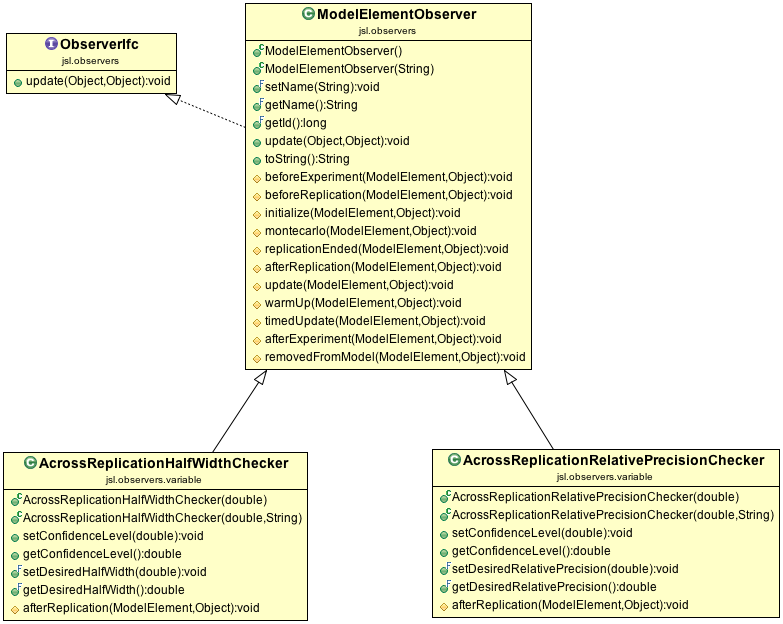
\includegraphics[width=0.8\linewidth,height=0.8\textheight]{./figures/ch7/ch7VariableObservers} \caption{Half-Width Observer Checking Code}\label{fig:HWChecker}
\end{figure}

Figure \ref{fig:HWChecker} presents part of the
\texttt{jsl.observers.variable} package which defines a base class called
\texttt{ModelElementObserver} that can be attached to instances of \texttt{ModelElement}
and then will be notified if various actions take place. There are a
number of actions associated with a \texttt{ModelElement} that occur during a
simulation that can be listened for by a \texttt{ModelElementObserver}:

\begin{itemize}
\item
  \texttt{beforeExperiment()} - This occurs prior to the first replication and
  before any events are executed.
\item
  \texttt{beforeReplication()} - This occurs prior to each replication and
  before any events are executed. The event calendar is cleared after
  this action.
\item
  \texttt{initialize()} - This occurs at the start of every replication (after
  beforeReplication() and after the event calendar is cleared) but
  before any events are executed. As we have seen, it is safe to
  schedule events in this method.
\item
  \texttt{warmUp()} - This occurs during a replication if a warm up period has
  been specified for the model. The statistical accumulators are
  cleared during this action if applicable.
\item
  \texttt{replicationEnded()} - This occurs at the end of every replication
  prior to the clearing of any statistical accumulators.
\item
  \texttt{afterReplication()} - This occurs at the end of every replication
  after the statistical accumulators have been cleared for the
  replication.
\item
  \texttt{afterExperiment()} - This occurs after all replications have been
  executed and prior to the end of the simulation.
\end{itemize}

\texttt{ModelElementObservers} are notified right \emph{after} the \texttt{ModelElement}
experiences the above mentioned actions. Thus, users of the
\texttt{ModelElementObserver} need to understand that the state of the model
element is available after the simulation actions of the model element
have occurred.

The \texttt{AcrossReplicationHalfWidthChecker} class listens to the
\texttt{afterReplication()} method of a \texttt{ResponseVariable} and checks the current
value of the half-width. This is illustrated in the following code listing.

\begin{Shaded}
\begin{Highlighting}[]
\KeywordTok{protected} \DataTypeTok{void} \FunctionTok{afterReplication}\OperatorTok{(}\NormalTok{ModelElement m}\OperatorTok{,} \BuiltInTok{Object}\NormalTok{ arg}\OperatorTok{)} \OperatorTok{\{}
\NormalTok{    ResponseVariable x }\OperatorTok{=} \OperatorTok{(}\NormalTok{ResponseVariable}\OperatorTok{)}\NormalTok{ m}\OperatorTok{;}
\NormalTok{    Simulation s }\OperatorTok{=}\NormalTok{ x}\OperatorTok{.}\FunctionTok{getSimulation}\OperatorTok{();}

    \ControlFlowTok{if} \OperatorTok{(}\NormalTok{s }\OperatorTok{==} \KeywordTok{null}\OperatorTok{)} \OperatorTok{\{}
        \ControlFlowTok{return}\OperatorTok{;}
    \OperatorTok{\}}
    \ControlFlowTok{if} \OperatorTok{(}\NormalTok{s}\OperatorTok{.}\FunctionTok{getCurrentReplicationNumber}\OperatorTok{()} \OperatorTok{\textless{}=} \FloatTok{2.0}\OperatorTok{)} \OperatorTok{\{}
        \ControlFlowTok{return}\OperatorTok{;}
    \OperatorTok{\}}

\NormalTok{    StatisticAccessorIfc stat }\OperatorTok{=}\NormalTok{ x}\OperatorTok{.}\FunctionTok{getAcrossReplicationStatistic}\OperatorTok{();}
    \DataTypeTok{double}\NormalTok{ hw }\OperatorTok{=}\NormalTok{ stat}\OperatorTok{.}\FunctionTok{getHalfWidth}\OperatorTok{(}\FunctionTok{getConfidenceLevel}\OperatorTok{());}
    \ControlFlowTok{if} \OperatorTok{(}\NormalTok{hw }\OperatorTok{\textless{}=}\NormalTok{ myDesiredHalfWidth}\OperatorTok{)} \OperatorTok{\{}
\NormalTok{        s}\OperatorTok{.}\FunctionTok{end}\OperatorTok{(}\StringTok{"Half{-}width condition met for "} \OperatorTok{+}\NormalTok{ x}\OperatorTok{.}\FunctionTok{getName}\OperatorTok{());}
    \OperatorTok{\}}
\OperatorTok{\}}
\end{Highlighting}
\end{Shaded}

Notice that a reference to the
observed \texttt{ResponseVariable} is used to get access to the across
replication statistics. If there are more than 2 replications, then the
half-width is checked against a user supplied desired half-width. If the
half-width criterion is met, then the simulation is told to end using
the \texttt{Simulation} class's \texttt{end()} method. The \texttt{end()} method causes the simulation to
not execute any future replications and to halt further execution.

The following code listing illustrates how to set up half-width
checking.

\begin{Shaded}
\begin{Highlighting}[]
\NormalTok{Simulation sim }\OperatorTok{=} \KeywordTok{new} \FunctionTok{Simulation}\OperatorTok{(}\StringTok{"LOTR Example"}\OperatorTok{);}
\CommentTok{// get the model}
\NormalTok{Model m }\OperatorTok{=}\NormalTok{ sim}\OperatorTok{.}\FunctionTok{getModel}\OperatorTok{();}
\CommentTok{// add system to the main model}
\NormalTok{LOTR system }\OperatorTok{=} \KeywordTok{new} \FunctionTok{LOTR}\OperatorTok{(}\NormalTok{m}\OperatorTok{,} \StringTok{"LOTR"}\OperatorTok{);}
\NormalTok{ResponseVariable rsv }\OperatorTok{=}\NormalTok{ m}\OperatorTok{.}\FunctionTok{getResponseVariable}\OperatorTok{(}\StringTok{"Time in RM and Inspection"}\OperatorTok{);}
\NormalTok{AcrossReplicationHalfWidthChecker hwc }\OperatorTok{=} \KeywordTok{new} \FunctionTok{AcrossReplicationHalfWidthChecker}\OperatorTok{(}\FloatTok{20.0}\OperatorTok{);}
\NormalTok{rsv}\OperatorTok{.}\FunctionTok{addObserver}\OperatorTok{(}\NormalTok{hwc}\OperatorTok{);}
\CommentTok{// set the parameters of the experiment}
\NormalTok{sim}\OperatorTok{.}\FunctionTok{setNumberOfReplications}\OperatorTok{(}\DecValTok{1000}\OperatorTok{);}
\BuiltInTok{System}\OperatorTok{.}\FunctionTok{out}\OperatorTok{.}\FunctionTok{println}\OperatorTok{(}\StringTok{"Simulation started."}\OperatorTok{);}
\NormalTok{sim}\OperatorTok{.}\FunctionTok{run}\OperatorTok{();}
\BuiltInTok{System}\OperatorTok{.}\FunctionTok{out}\OperatorTok{.}\FunctionTok{println}\OperatorTok{(}\StringTok{"Simulation completed."}\OperatorTok{);}
\NormalTok{sim}\OperatorTok{.}\FunctionTok{printHalfWidthSummaryReport}\OperatorTok{();}
\end{Highlighting}
\end{Shaded}

All that is needed is to get a reference to the response
variable that needs to be check so that the observer can be attached.
This can be done easily in the location of the code where the response
variable is created or as in this example, the name of the response
variable is used to get the reference from the model. Line~6 of the
listing illustrates using the name to get the reference, followed by the
construction of the checker (line~7) and attaching it as an observer
(line~8).

In the sequential sampling experiment there were 66 replications. This
is actually more than the recommended 61 replications for the fixed
half-width method. This is perfectly possible, and emphasizes the fact
that in the sequential sampling method, the number of replications is
actually a random variable. If you were to use different streams and
re-run the sequential sampling experiment, the number of replications
completed may be different each time.

\begin{longtable}[]{@{}lcc@{}}
\caption{Half-Width Summary Report for Sequential Analysis}\tabularnewline
\toprule
Response Name & \(\bar{x}\) & \(hw\) \\
\midrule
\endfirsthead
\toprule
Response Name & \(\bar{x}\) & \(hw\) \\
\midrule
\endhead
RingMakingStation:R:Util & 0.981083 & 0.002039 \\
RingMakingStation:R:BusyUnits & 0.981083 & 0.002039 \\
RingMakingStation:Q:Num In Q & 37.364044 & 1.963297 \\
RingMakingStation:Q:Time In Q & 380.608370 & 19.903070 \\
RingMakingStation:NS & 38.345127 & 1.964300 \\
InspectStation:R:Util & 0.426379 & 0.005022 \\
InspectStation:R:BusyUnits & 0.426379 & 0.005022 \\
InspectStation:Q:Num In Q & 0.000948 & 0.000263 \\
InspectStation:Q:Time In Q & 0.009558 & 0.002622 \\
InspectStation:NS & 0.427327 & 0.005109 \\
ReworkStation:R:Util & 0.127123 & 0.011491 \\
ReworkStation:R:BusyUnits & 0.127123 & 0.011491 \\
ReworkStation:Q:Num In Q & 0.004093 & 0.001949 \\
ReworkStation:Q:Time In Q & 0.530734 & 0.255424 \\
ReworkStation:NS & 0.131216 & 0.012288 \\
PackingStation:R:Util & 0.687782 & 0.006946 \\
PackingStation:R:BusyUnits & 0.687782 & 0.006946 \\
PackingStation:Q:Num In Q & 0.103600 & 0.008483 \\
PackingStation:Q:Time In Q & 1.050310 & 0.080851 \\
PackingStation:NS & 0.791382 & 0.013703 \\
System Time & 404.357533 & 19.948930 \\
Num in System & 39.695052 & 1.969934 \\
Prob too Big & 0.031764 & 0.004634 \\
Prob too Small & 0.038146 & 0.004449 \\
Prob of Over Time & 0.106061 & 0.076275 \\
Time to Make Orders & 782.451179 & 39.996433 \\
Num in RM and Inspection & 38.772454 & 1.964935 \\
Time in RM and Inspection & 394.965666 & 19.914630 \\
Across Rep Stat Num Completed & 76.803030 & 3.936414 \\
Number of replications: 66 & & \\
\bottomrule
\end{longtable}

\hypertarget{simoa:infhorizon}{%
\section{Analysis of Infinite Horizon Simulations}\label{simoa:infhorizon}}

This section discusses how to plan and analyze infinite horizon
simulations. When analyzing infinite horizon simulations, the primary
difficulty is the nature of within replication data. In the finite
horizon case, the statistical analysis is based on three basic
requirements:

\begin{enumerate}
\def\labelenumi{\arabic{enumi}.}
\item
  Observations are independent
\item
  Observations are sampled from identical distributions
\item
  Observations are drawn from a normal distribution (or enough
  observations are present to invoke the central limit theorem)
\end{enumerate}

These requirements were met by performing independent replications of
the simulation to generate a random sample. In a direct sense, the
data within a replication do not satisfy any of these requirements;
however, certain procedures can be imposed on the manner in which the
observations are gathered to ensure that these statistical assumptions
are not grossly violated. The following will first explain why within
replication data typically violates these assumptions and then will
provide some methods for mitigating the violations within the context of
infinite horizon simulations.

To illustrate the challenges related to infinite horizon simulations, a
simple spreadsheet simulation was developed for a M/M/1 queue.

\begin{figure}
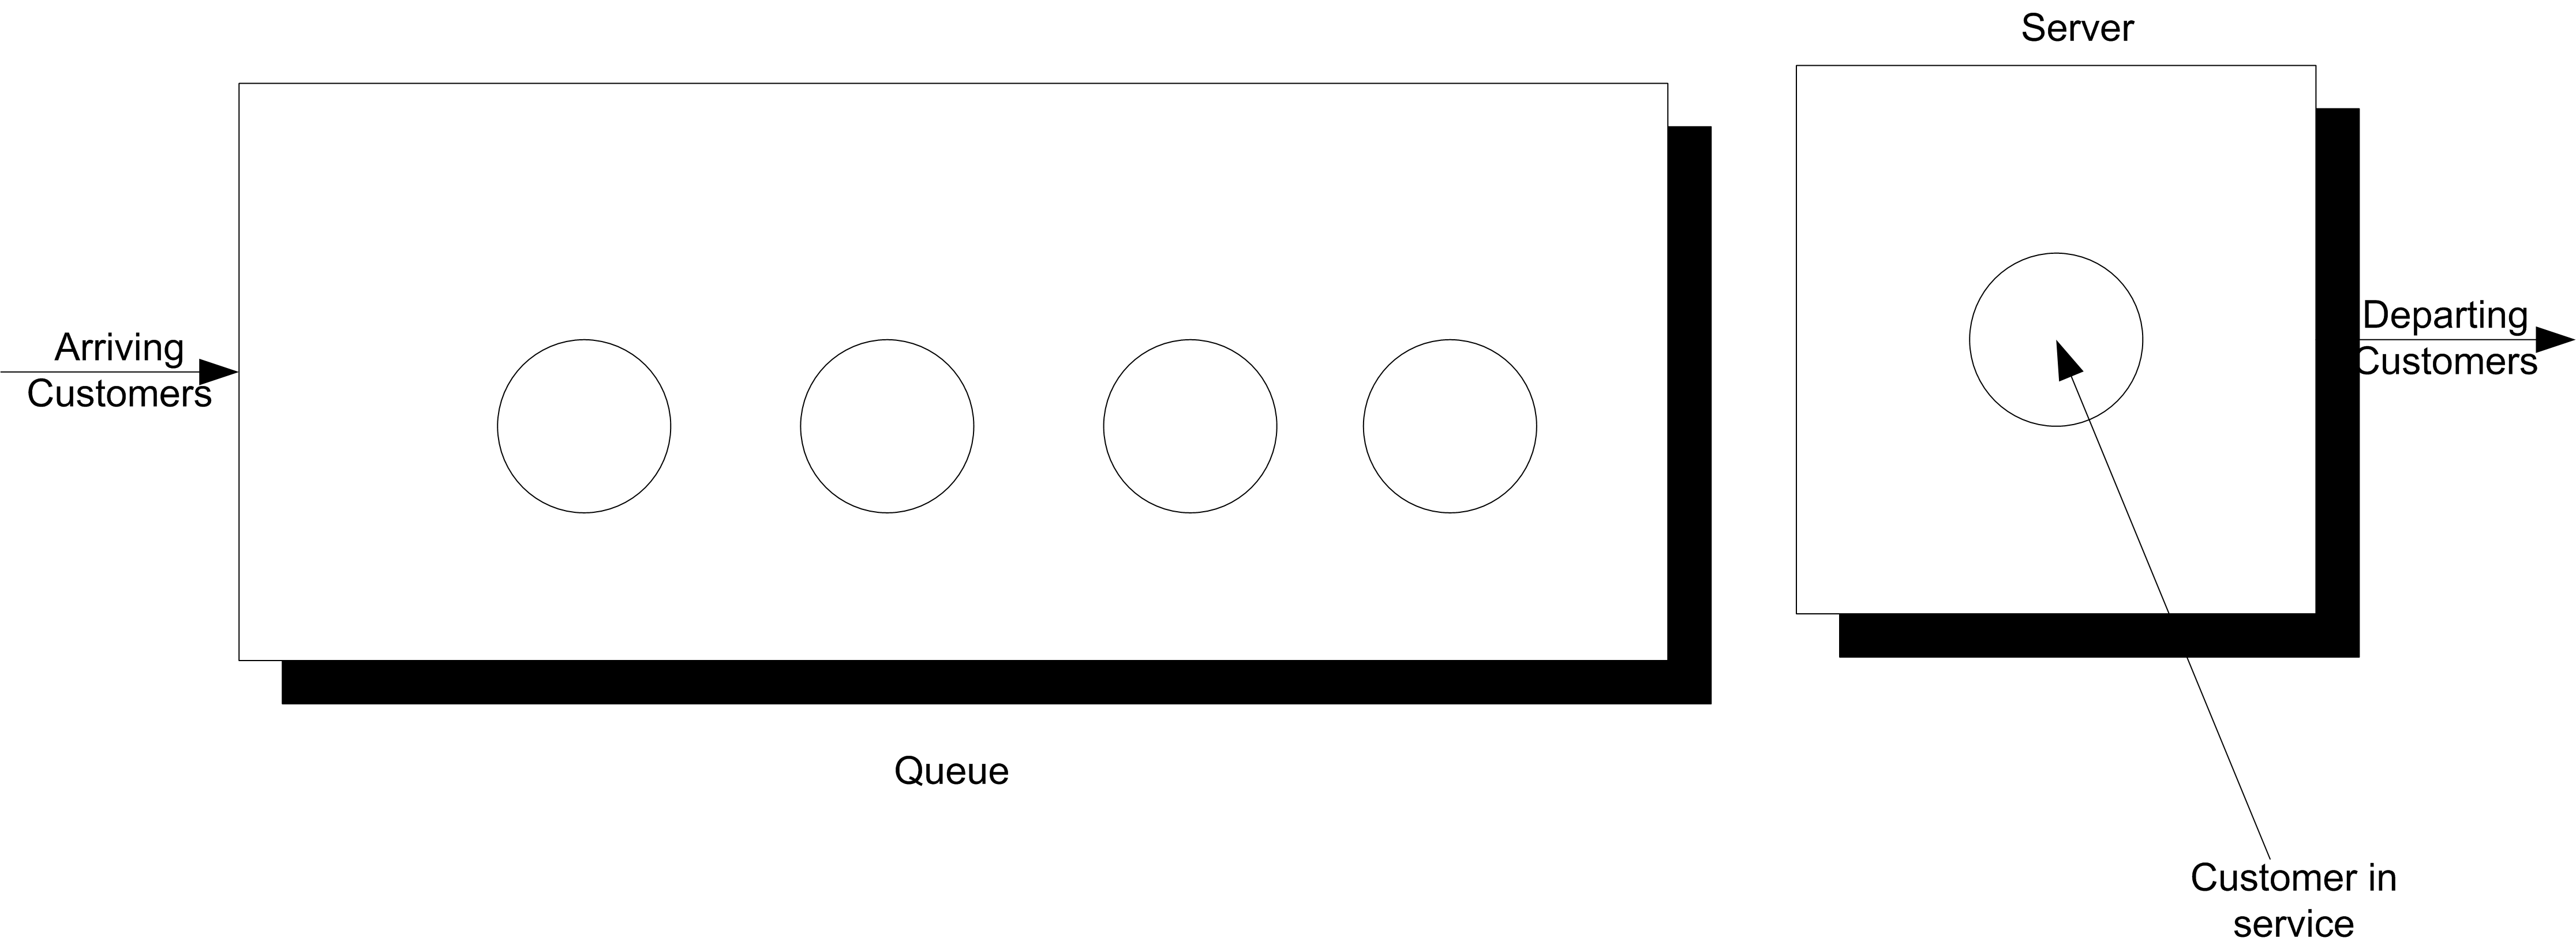
\includegraphics[width=0.8\linewidth,height=0.8\textheight]{./figures/ch7/ch7fig30} \caption{Single Server Queueing System}\label{fig:SingleServer}
\end{figure}

Consider a single server queuing system as illustrated Figure \ref{fig:SingleServer}.

For a single server queueing system, there is an equation that allows
the computation of the waiting times of each of the customers based on
knowledge of the arrival and service times. Let \(X_1, X_2, \ldots\)
represent the successive service times and \(Y_1, Y_2, \ldots\) represent
the successive inter-arrival times for each of the customers that visit
the queue. Let \(E[Y_i] = 1/\lambda\) be the mean of the inter-arrival
times so that \(\lambda\) is the mean arrival rate. Let \(E[Y_i] = 1/\mu\)
be the mean of the service times so that \(\mu\) is the mean service rate.
Let \(W_i\) be the waiting time in the queue for the \(i^{th}\) customer.
That is, the time between when the customer arrives until they enter
service.

Lindley's equation, see \citep{gross1998fundamentals}, relates the waiting
time to the arrivals and services as follows:

\[W_{i+1} = max(0, W_i + X_i - Y_i)\]

The relationship says that the time that the \((i + 1)^{st}\) customer
must wait is the time the \(i^{th}\) waited, plus the \(i^{th}\) customer's
service time, \(X_i\) (because that customer is in front of the \(i^{th}\)
customer), less the time between arrivals of the \(i^{th}\) and
\((i + 1)^{st}\) customers, \(Y_i\). If \(W_i + X_i - Y_i\) is less than zero,
then the (\((i + 1)^{st}\) customer arrived after the \(i^{th}\) finished
service, and thus the waiting time for the \((i + 1)^{st}\) customer is
zero, because his service starts immediately.

Suppose that \(X_i \sim exp(E[X_i] = 0.7)\) and
\(Y_i \sim exp(E[Y_i] = 1.0)\). This is a M/M/1 queue with \(\lambda\) = 1
and \(\mu\) = 10/7. Thus, based on traditional queuing theory results:

\[\rho = 0.7\]

\[L_q = \dfrac{0.7 \times 0.7}{1 - 0.7} = 1.6\bar{33}\]

\[W_q = \dfrac{L_q}{\lambda} = 1.6\bar{33} \; \text{minutes}\]

Lindley's equation can be readily implemented in Java as illustrated in the following code listing.

\begin{Shaded}
\begin{Highlighting}[]
\CommentTok{// inter{-}arrival time distribution}
\NormalTok{RandomIfc y }\OperatorTok{=} \KeywordTok{new} \FunctionTok{ExponentialRV}\OperatorTok{(}\FloatTok{1.0}\OperatorTok{);}
\CommentTok{// service time distribution}
\NormalTok{RandomIfc x }\OperatorTok{=} \KeywordTok{new} \FunctionTok{ExponentialRV}\OperatorTok{(}\FloatTok{0.7}\OperatorTok{);}
\DataTypeTok{int}\NormalTok{ r }\OperatorTok{=} \DecValTok{30}\OperatorTok{;} \CommentTok{// number of replications}
\DataTypeTok{int}\NormalTok{ n }\OperatorTok{=} \DecValTok{100000}\OperatorTok{;} \CommentTok{// number of customers}
\DataTypeTok{int}\NormalTok{ d }\OperatorTok{=} \DecValTok{10000}\OperatorTok{;} \CommentTok{// warm up}
\NormalTok{Statistic avgw }\OperatorTok{=} \KeywordTok{new} \FunctionTok{Statistic}\OperatorTok{(}\StringTok{"Across rep avg waiting time"}\OperatorTok{);}
\NormalTok{Statistic wbar }\OperatorTok{=} \KeywordTok{new} \FunctionTok{Statistic}\OperatorTok{(}\StringTok{"Within rep avg waiting time"}\OperatorTok{);}
\ControlFlowTok{for} \OperatorTok{(}\DataTypeTok{int}\NormalTok{ i }\OperatorTok{=} \DecValTok{1}\OperatorTok{;}\NormalTok{ i }\OperatorTok{\textless{}=}\NormalTok{ r}\OperatorTok{;}\NormalTok{ i}\OperatorTok{++)} \OperatorTok{\{}
    \DataTypeTok{double}\NormalTok{ w }\OperatorTok{=} \DecValTok{0}\OperatorTok{;} \CommentTok{// initial waiting time}
    \ControlFlowTok{for} \OperatorTok{(}\DataTypeTok{int}\NormalTok{ j }\OperatorTok{=} \DecValTok{1}\OperatorTok{;}\NormalTok{ j }\OperatorTok{\textless{}=}\NormalTok{ n}\OperatorTok{;}\NormalTok{ j}\OperatorTok{++)} \OperatorTok{\{}
\NormalTok{        w }\OperatorTok{=} \BuiltInTok{Math}\OperatorTok{.}\FunctionTok{max}\OperatorTok{(}\FloatTok{0.0}\OperatorTok{,}\NormalTok{ w }\OperatorTok{+}\NormalTok{ x}\OperatorTok{.}\FunctionTok{getValue}\OperatorTok{()} \OperatorTok{{-}}\NormalTok{ y}\OperatorTok{.}\FunctionTok{getValue}\OperatorTok{());}
\NormalTok{        wbar}\OperatorTok{.}\FunctionTok{collect}\OperatorTok{(}\NormalTok{w}\OperatorTok{);}\CommentTok{// collect waiting time}
        \ControlFlowTok{if} \OperatorTok{(}\NormalTok{j }\OperatorTok{==}\NormalTok{ d}\OperatorTok{)} \OperatorTok{\{}\CommentTok{// clear stats at warmup}
\NormalTok{            wbar}\OperatorTok{.}\FunctionTok{reset}\OperatorTok{();}
        \OperatorTok{\}}
    \OperatorTok{\}}
    \CommentTok{//collect across replication statistics}
\NormalTok{    avgw}\OperatorTok{.}\FunctionTok{collect}\OperatorTok{(}\NormalTok{wbar}\OperatorTok{.}\FunctionTok{getAverage}\OperatorTok{());}
    \CommentTok{// clear within replication statistics for next rep}
\NormalTok{    wbar}\OperatorTok{.}\FunctionTok{reset}\OperatorTok{();}
\OperatorTok{\}}
\BuiltInTok{System}\OperatorTok{.}\FunctionTok{out}\OperatorTok{.}\FunctionTok{println}\OperatorTok{(}\StringTok{"Replication/Deletion Lindley Equation Example"}\OperatorTok{);}
\BuiltInTok{System}\OperatorTok{.}\FunctionTok{out}\OperatorTok{.}\FunctionTok{println}\OperatorTok{(}\NormalTok{avgw}\OperatorTok{);}
\end{Highlighting}
\end{Shaded}

This implementation can be readily extended to capture the data to files for display in spreadsheets or other plotting software. As part of the plotting process it is useful to display the cumulative sum and cumulative average of the data values.

\[\sum_{i=1}^n W_i \; \text{for} \; n = 1,2,\ldots\]

\[\dfrac{1}{n} \sum_{i=1}^n W_i \; \text{for} \; n = 1,2,\ldots\]

\begin{figure}
\centering
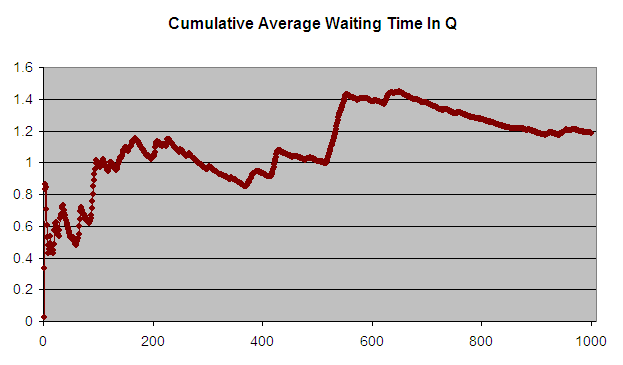
\includegraphics{./figures/ch7/ch7fig34.png}
\caption{\label{fig:CumulativeAvg}Cumulative Average Waiting Time of 1000 Customers}
\end{figure}

Figure \ref{fig:CumulativeAvg} presents the cumulative average plot
of the first 1000 customers. As seen in the plot, the cumulative average
starts out low and then eventually trends towards 1.2 minutes.

\begin{figure}
\centering
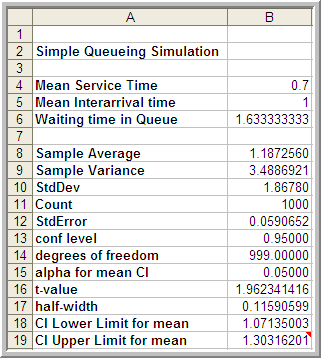
\includegraphics{./figures/ch7/ch7fig33.png}
\caption{\label{fig:MM1Results1000}Lindley Equation Results Across 1000 Customers}
\end{figure}

The analytical results indicate that the true
long-run expected waiting time in the queue is 1.633 minutes. The
average over the 1000 customers in the simulation is 1.187 minutes. The results in Figure \ref{fig:MM1Results1000} indicated that the sample average is
significantly lower than the true expected average. We will explore why this occurs shortly.

The first issue to consider with this data is independence. To do this
you should analyze the 1000 observations in terms of its
autocorrelation.

\begin{figure}
\centering
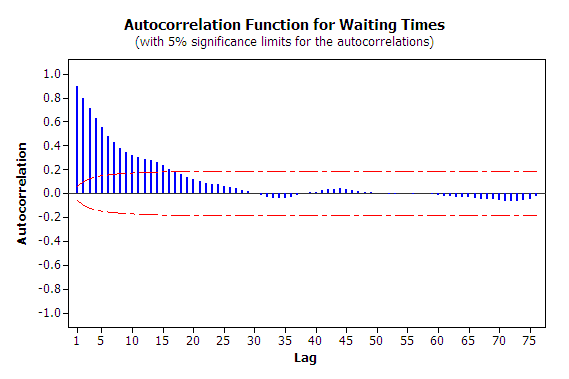
\includegraphics{./figures/ch7/ch7fig35.png}
\caption{\label{fig:MM1Autocorelation}Autocorrelation Plot for Waiting Times}
\end{figure}

From Figure \ref{fig:MM1Autocorelation}, it is readily apparent that the
data has strong positive correlation. The lag-1
correlation for this data is estimated to be about 0.9.
Figure \ref{fig:MM1Autocorelation} clearly indicates the strong first
order linear dependence between \(W_i\) and \(W_{i-1}\). This positive
dependence implies that if the previous customer waited a long time the
next customer is likely to wait a long time. If the previous customer
had a short wait, then the next customer is likely to have a short wait.
This makes sense with respect to how a queue operates.

Strong positive correlation has serious implications when developing
confidence intervals on the mean customer waiting time because the usual
estimator for the sample variance:

\[S^2(n) = \dfrac{1}{n - 1} \sum_{i=1}^n (X_i - \bar{X})^2\]

is a biased estimator for the true population variance when there is
correlation in the observations. This issue will be re-examined when
ways to mitigate these problems are discussed.

The second issue that needs to be discussed is that of the
non-stationary behavior of the data. Non-stationary data indicates some dependence on time. More generally, non-stationary implies that the \(W_1, W_2,W_3, \ldots, W_n\) are not
obtained from identical distributions.

Why should the distribution of \(W_1\) not be the same as the distribution
of \(W_{1000}\)? The first customer is likely to enter the queue with no
previous customers present and thus it is very likely that the first
customer will experience little or no wait (the way \(W_0\) was initialize
in this example allows a chance of waiting for the first customer).
However, the \(1000^{th}\) customer may face an entirely different
situation. Between the \(1^{st}\) and the \(1000^{th}\) customer there might
likely be a line formed. In fact from the M/M/1 formula, it is known
that the steady state expected number in the queue is 1.633. Clearly,
the conditions that the \(1^{st}\) customer faces are different than the
\(1000^{th}\) customer. Thus, the distributions of their waiting times are
likely to be different.

This situation can be better understood by considering a model for the underlying data. A time
series, \(X_1,X_2,\ldots,\) is said to be \emph{covariance stationary} if:

\begin{itemize}
\item
  The mean exists and \(\theta = E[X_i]\), for i = 1,2,\(\ldots\), n
\item
  The variance exists and \(Var[X_i] = \sigma^2\) \(>\) 0, for i =
  1,2,\(\ldots\), n
\item
  The lag-k autocorrelation, \(\rho_k = cor(X_i, X_{i+k})\), is not a
  function of \emph{i}, i.e.~the correlation between any two points in the
  series does not depend upon where the points are in the series, it
  depends only upon the distance between them in the series.
\end{itemize}

In the case of the customer waiting times, we can conclude from the
discussion that it is very likely that \(\theta \neq E[X_i]\) and
\(Var[X_i] \neq \sigma^2\) for \emph{each} i = 1,2,\(\ldots\), n for the time
series.

Do you think that is it likely that the distributions of \(W_{9999}\) and
\(W_{10000}\) will be similar? The argument, that the \(9999^{th}\) customer
is on average likely to experience similar conditions as the
\(10000^{th}\) customer, sure seems reasonable.

\begin{figure}
\centering
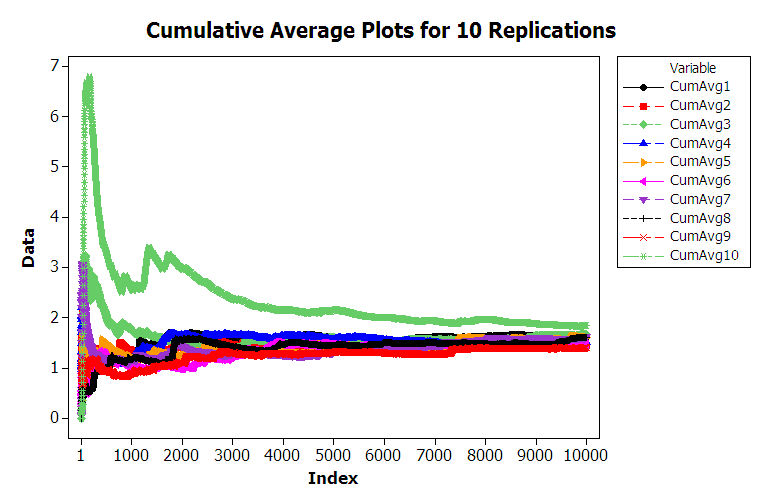
\includegraphics{./figures/ch7/ch7fig37.png}
\caption{\label{fig:MM1MutipleSP}Multiple Sample Paths of Queueing Simulation}
\end{figure}

Figure \ref{fig:MM1MutipleSP} shows 10 different replications of
the cumulative average for a 10000 customer simulation. From the figure, we can see that the cumulative average plots can vary significantly over the 10000 customers with the average tracking above
the true expected value, below the true expected value, and possibly
towards the true expected value. For the case of 10000 customers, you should notice
that the cumulative average starts to approach the expected value of the
steady state mean waiting time in the queue with increasing number of
customers. This is the law of large numbers in action. It appears that
it takes a period of time for the performance measure to \emph{warm up}
towards the true mean. Determining the warm up time will be the basic
way to mitigate the problem of this non-stationary behavior.

From this discussion, we can conclude that the second basic
statistical assumption of identically distributed data is not valid for
within replication data. From this, we can also conclude that it is
very likely that the data are not normally distributed. In fact, for the
M/M/1 it can be shown that the steady state distribution for the waiting
time in the queue is not a normal distribution. Thus, all three of the
basic statistical assumptions are violated for the within replication
data of this example. This problem needs to be addressed in order to
properly analyze infinite horizon simulations.

There are two basic methods for performing infinite horizon simulations.
The first is to perform multiple replications. This approach addresses
independence and normality in a similar fashion as the finite horizon
case, but special procedures will be needed to address the
non-stationary aspects of the data. The second basic approach is to work
with one very long replication. Both of these methods depend on first
addressing the problem of the non-stationary aspects of the data. The
next section looks at ways to mitigate the non-stationary aspect of
within-replication data for infinite horizon simulations.

\hypertarget{simoa:infhorizon:initialbias}{%
\subsection{Assessing the Effect of Initial Conditions}\label{simoa:infhorizon:initialbias}}

Consider the output stochastic process \(X_i\) of the simulation. Let
\(F_i(x|I)\) be the conditional cumulative distribution function of \(X_i\)
where \(I\) represents the initial conditions used to start the simulation
at time 0. If \(F_i(x|I) \rightarrow F(x)\) when \(i \rightarrow \infty\),
for all initial conditions \(I\), then \(F(x)\) is called the steady state
distribution of the output process. (Law 2007).

In infinite horizon simulations, estimating parameters of the steady
state distribution, \(F(x)\), such as the steady state mean, \(\theta\), is
often the key objective. The fundamental difficulty associated with
estimating steady state performance is that unless the system is
initialized using the steady state distribution (which is not known),
there is no way to directly observe the steady state distribution.

It is true that if the steady state distribution exists and you run the
simulation long enough the estimators will tend to converge to the
desired quantities. Thus, within the infinite horizon simulation
context, you must decide on how long to run the simulations and how to
handle the effect of the \emph{initial conditions} on the estimates of
performance. The initial conditions of a simulation represent the state
of the system when the simulation is started. For example, in simulating
the pharmacy system, the simulation was started with no customers in
service or in the line. This is referred to as \emph{empty and idle}. The
initial conditions of the simulation affect the rate of convergence of
estimators of steady state performance.

Because the distributions \(F_i(x|I)\) at the start of the replication
tend to depend more heavily upon the initial conditions, estimators of
steady state performance such as the sample average, \(\bar{X}\), will
tend to be \emph{biased}. A point estimator, \(\hat{\theta}\), is an \emph{unbiased}
estimator of the parameter of interest, \(\theta\), if
\(E[\hat{\theta}] = \theta\). That is, if the expected value of the
sampling distribution is equal to the parameter of interest then the
estimator is said to be unbiased. If the estimator is biased then the
difference, \(E[\hat{\theta}] - \theta\), is called the bias of,
\(\hat{\theta}\), the estimator.

Note that any individual difference between the true parameter,
\(\theta\), and a particular observation, \(X_i\), is called error,
\(\epsilon_i = X_i -\theta\). If the expected value of the errors is not
zero, then there is bias. A particular observation is not biased. Bias
is a property of the estimator. Bias is analogous to being consistently
off target when shooting at a bulls-eye. It is as if the sights on your
gun are crooked. In order to estimate the bias of an estimator, you must
have multiple observations of the estimator. Suppose that you are
estimating the mean waiting time in the queue as per the previous
example and that the estimator is based on the first 20 customers. That
is, the estimator is:

\[\bar{W}_r = \dfrac{1}{20}\sum_{i=1}^{20} W_{ir}\]

and there are \(r = 1, 2, \ldots 10\) replications.
The following table shows the sample average waiting time for the
first 20 customers for 10 different replications.

\begin{longtable}[]{@{}ccc@{}}
\caption{Ten Replications of 20 Customers}\tabularnewline
\toprule
r & \(\bar{W}_r\) & \(B_r = \bar{W}_r - W_q\) \\
\midrule
\endfirsthead
\toprule
r & \(\bar{W}_r\) & \(B_r = \bar{W}_r - W_q\) \\
\midrule
\endhead
1 & 0.194114 & -1.43922 \\
2 & 0.514809 & -1.11852 \\
3 & 1.127332 & -0.506 \\
4 & 0.390004 & -1.24333 \\
5 & 1.05056 & -0.58277 \\
6 & 1.604883 & -0.02845 \\
7 & 0.445822 & -1.18751 \\
8 & 0.610001 & -1.02333 \\
9 & 0.52462 & -1.10871 \\
~10 & 0.335311 & -1.29802 \\
& \(\bar{\bar{W}}\) = 0.6797 & \(\bar{B}\) = -0.9536 \\
\bottomrule
\end{longtable}

In the table, \(B_r\) is an estimate of the bias for the \(r^{th}\) replication, where
\(W_q = 1.6\bar{33}\). Upon averaging across the replications, it can be
seen that \(\bar{B}= -0.9536\), which indicates that the estimator based
only on the first 20 customers has significant negative bias, i.e.~on
average it is less than the target value.

This is the so called \emph{initialization bias problem} in steady state
simulation. Unless the initial conditions of the simulation can be
generated according to \(F(x)\), which is not known, you must focus on
methods that detect and/or mitigate the presence of initialization bias.

One strategy for initialization bias mitigation is to find an index,
\(d\), for the output process, \({X_i}\), so that \({X_i; i = d + 1, \ldots}\)
will have substantially similar distributional properties as the steady
state distribution \(F(x)\). This is called the simulation warm up
problem, where \(d\) is called the warm up point, and \({i = 1,\ldots,d}\)
is called the warm up period for the simulation. Then, the estimators of
steady state performance are based only on \({X_i; i = d + 1, \ldots}\),
which represent the data after deleting the warm up period.

For example, when estimating the steady state mean waiting time for each
replication \(r\) the estimator would be:

\[\bar{W_r} = \dfrac{1}{n-d}\sum_{i=d+1}^{n} W_{ir}\]

For time-based performance measures, such as the average number in
queue, a time \(T_w\) can be determined past which the data collection
process can begin. Estimators of time-persistent performance such as the
sample average are computed as:

\[\bar{Y}_r = \dfrac{1}{T_e - T_w}\int_{T_w}^{T_e} Y_r(t) dt\]

\begin{figure}
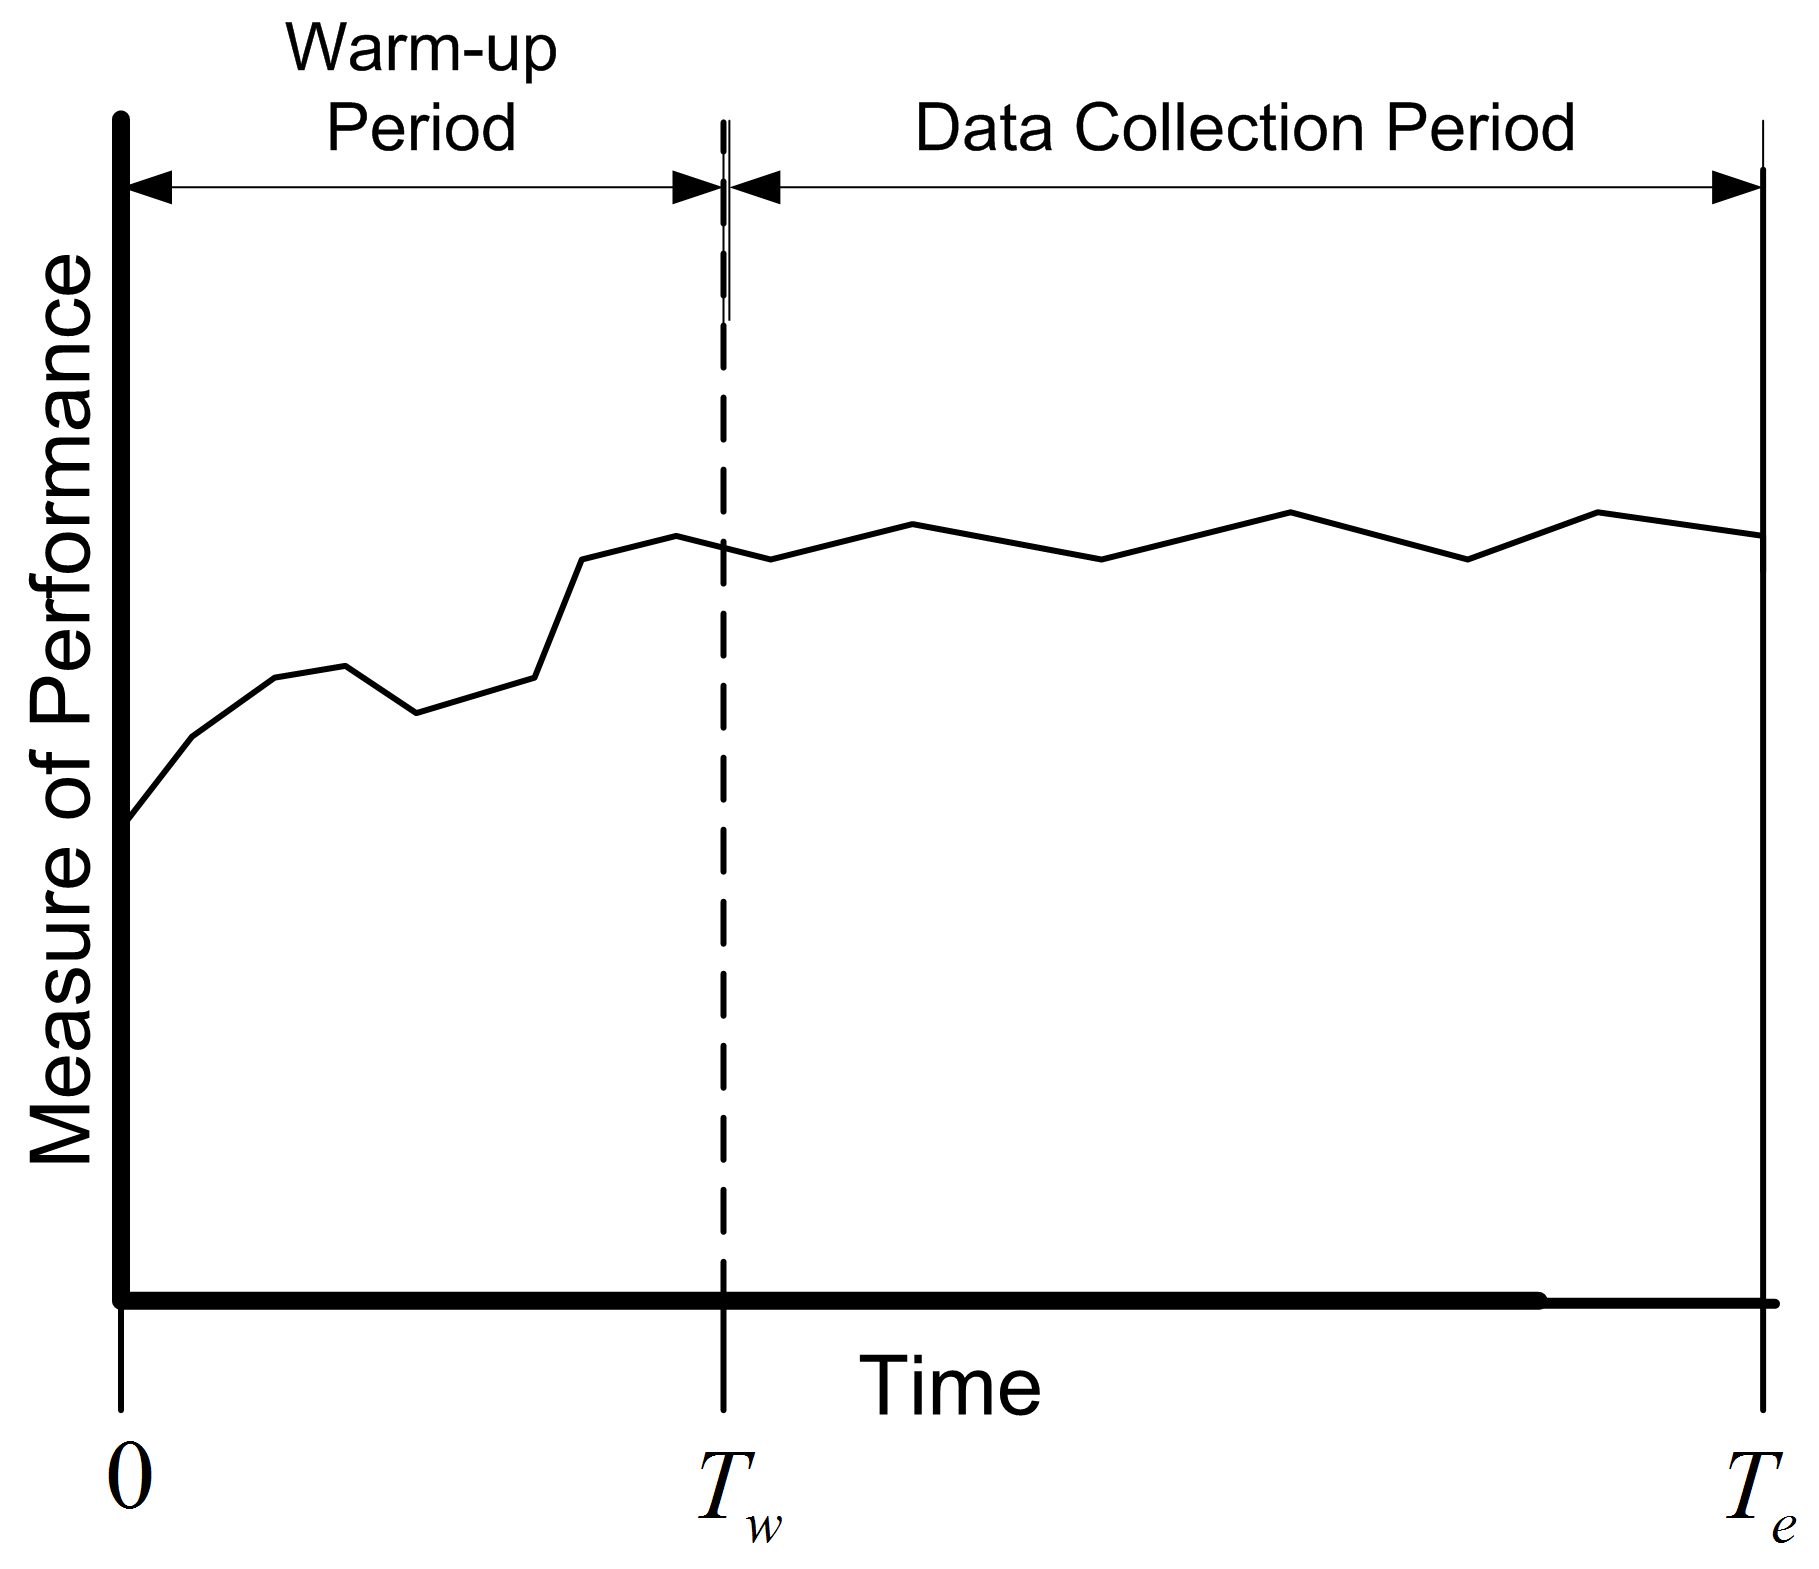
\includegraphics[width=0.8\linewidth,height=0.8\textheight]{./figures/ch7/ch7fig38} \caption{The Concept of the Warm Up Period}\label{fig:WarmUpPeriod}
\end{figure}

Figure \ref{fig:WarmUpPeriod} shows the concept of a warm up period for a
simulation replication. When you perform a simulation, you can easily
specify a time-based warm up period using the setLengthOfWarmUp() method
of the Simulation class. In fact, even for observation based data, it
will be more convenient to specify the warm up period in terms of time.
A given value of \(T_w\) implies a particular value of \(d\) and vice a
versa. Specifying a warm up period, causes an event to be scheduled for
time \(T_w\). At that time, all the accumulated statistical counters are
cleared so that the net effect is that statistics are only collected
over the period from \(T_w\) to \(T_e\). The problem then becomes that of
finding an appropriate warm up period.

Before proceeding with how to assess the length of the warm up period,
the concept of steady state needs to be further examined. This subtle
concept is often misunderstood or misrepresented. Often you will hear
the phrase: \emph{The system has reached steady state}. The correct
interpretation of this phrase is that the distribution of the desired
performance measure has reached a point where it is sufficiently similar
to the desired steady state distribution. Steady state is a concept
involving the performance measures generated by the system as time goes
to infinity. However, sometimes this phrase is interpreted incorrectly
to mean that the system \emph{itself} has reached steady state. Let me state
emphatically that the system \emph{never} reaches steady state. If the system
itself reached steady state, then by implication it would never change
with respect to time. It should be clear that the system continues to
evolve with respect to time; otherwise, it would be a very boring
system! Thus, it is incorrect to indicate that the system has reached
steady state. Because of this, do not to use the phrase: \emph{The system has
reached steady state}.

Understanding this subtle issue raises an interesting implication
concerning the notion of deleting data to remove the initialization
bias. Suppose that the state of the system at the end of the warm up
period, \(T_w\), is exactly the same as at \(T = 0\). For example, it is
certainly possible that at time \(T_w\) for a particular replication that
the system was empty and idle. Since the state of the system at \(T_w\) is
the same as that of the initial conditions, there will be no effect of
deleting the warm up period for this replication. In fact there will be
a negative effect, in the sense that data will have been thrown away for
no reason. Deletion methods are predicated on the likelihood that the
state of the system seen at \(T_w\) is more representative of steady state
conditions. At the end of the warm up period, the system can be in \emph{any
of the possible} states of the system. Some states will be more likely
than others. If multiple replications are made, then at \(T_w\) each
replication will experience a different set of conditions at \(T_w\). Let
\(I_{T_w}^r\) be the initial conditions (state) at time \(T_w\) on
replication \(r\). By setting a warm up period and performing multiple
replications, you are in essence sampling from the distribution
governing the state of the system at time \(T_w\). If \(T_w\) is long
enough, then on average across the replications, you are more likely to
start collecting data when the system is in states that are more
representative over the long term (rather than just empty and idle).

Many methods and rules have been proposed to determine the warm up
period. The interested reader is referred to \citep{wilson1978a}, \citet{lada2003a},
\citep{Litton:2002aa}, \citet{white2000a}, \citet{cash1992}, and \citep{rossetti1995control} for
an overview of such methods. This discussion will concentrate on the
visual method proposed in \citep{welch1983a}.

The basic idea behind Welch's graphical procedure is simple:

\begin{itemize}
\item
  Make \(R\) replications. Typically, \(R \geq 5\) is recommended.
\item
  Let \(Y_{rj}\) be the \(j^{th}\) observation on replication \(r\) for
  \(j = 1,2,\cdots,m_r\) where \(m_r\) is the number of observations in
  the \(r^{th}\) replication, and \(r = 1,2,\cdots,n\),
\item
  Compute the averages across the replications for each
  \(j = 1, 2, \ldots, m\), where \(m = min(m_r)\) for \(r = 1,2,\cdots,n\).

  \[\bar{Y}_{\cdot j} = \dfrac{1}{n}\sum_{r=1}^n Y_{rj}\]
\item
  Plot, \(\bar{Y}_{\cdot j}\) for each \(j = 1, 2, \ldots, m\)
\item
  Apply smoothing techniques to \(\bar{Y}_{\cdot j}\) for
  \(j = 1, 2, \ldots, m\)
\item
  Visually assess where the plots start to converge
\end{itemize}

Let's apply the Welch's procedure to the replications generated from the
Lindley equation simulation. Using the 10 replications stored in a spreadsheet
we can compute the average across each replication for each
customer.

\begin{figure}
\centering
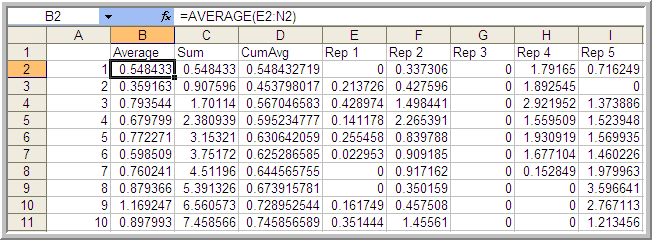
\includegraphics{./figures/ch7/ch7fig39.png}
\caption{\label{fig:WelchPlot}Computing the Averages for the Welch Plot}
\end{figure}

In Figure \ref{fig:WelchPlot}, cell B2 represents the average across the
10 replications for the \(1^{st}\) customer. Column D represents the
cumulative average associated with column B.

\begin{figure}
\centering
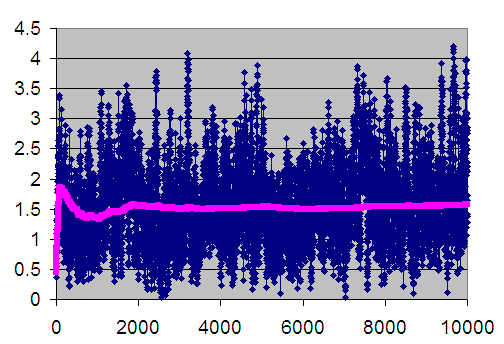
\includegraphics{./figures/ch7/ch7fig40.png}
\caption{\label{fig:CumAvgline}Welch Plot with Superimposed Cumulative Average Line}
\end{figure}

Figure \ref{fig:CumAvgline} is the plot of the cumulative average
(column D) superimposed on the averages across replications (column B).
The cumulative average is one method of smoothing the data. From the
plot, you can infer that after about customer 3000 the cumulative
average has started to converge. Thus, from this analysis you might
infer that \(d = 3000\).

When you perform an infinite horizon simulation by specifying a warm up
period and making multiple replications, you are using the method of
\emph{replication-deletion.} If the method of replication-deletion with
\(d = 3000\) is used for the current example, a slight reduction in the
bias can be achieved as indicated in the following table.

\begin{longtable}[]{@{}ccccc@{}}
\caption{Replication-Deletion Results, d = 3000}\tabularnewline
\toprule
\(r\) & \(\bar{W}_r\) \((d = 0)\) & \(\bar{W}_r(d = 3000)\) & \(B_r(d = 0)\) & \(B_r(d = 3000)\) \\
\midrule
\endfirsthead
\toprule
\(r\) & \(\bar{W}_r\) \((d = 0)\) & \(\bar{W}_r(d = 3000)\) & \(B_r(d = 0)\) & \(B_r(d = 3000)\) \\
\midrule
\endhead
1 & 1.594843 & 1.592421 & -0.03849 & -0.04091 \\
2 & 1.452237 & 1.447396 & -0.1811 & -0.18594 \\
3 & 1.657355 & 1.768249 & 0.024022 & 0.134915 \\
4 & 1.503747 & 1.443251 & -0.12959 & -0.19008 \\
5 & 1.606765 & 1.731306 & -0.02657 & 0.097973 \\
6 & 1.464981 & 1.559769 & -0.16835 & -0.07356 \\
7 & 1.621275 & 1.75917 & -0.01206 & 0.125837 \\
8 & 1.600563 & 1.67868 & -0.03277 & 0.045347 \\
9 & 1.400995 & 1.450852 & -0.23234 & -0.18248 \\
10 & 1.833414 & 1.604855 & 0.20008 & -0.02848 \\
& \(\bar{\bar{W}}\) = 1.573617 & \(\bar{\bar{W}}\) = 1.603595 & \(\bar{B}\) = -0.05972 & \(\bar{B}\) = -0.02974 \\
& s = 0.1248 & s = 0.1286 & s = 0.1248 & s = 0.1286 \\
95\% LL & 1.4843 & 1.5116 & -0.149023 & -0.121704 \\
95\% UL & 1.6629 & 1.6959 & -0.029590 & 0.062228 \\
\bottomrule
\end{longtable}

While not definitive for this simple example, the results suggest that
deleting the warm up period helps to reduce initialization bias. This
model's warm up period will be further analyzed using additional tools
available in the next section.

In performing the method of replication-deletion, there is a fundamental
trade-off that occurs. Because data is deleted, the variability of the
estimator will tend to increase while the bias will tend to decrease.
This is a trade-off between a reduction in bias and an increase in
variance. That is, accuracy is being traded off against precision when
deleting the warm up period. In addition to this trade off, data from
each replication is also being thrown away. This takes computational
time that could be expended more effectively on collecting usable data.
Another disadvantage of performing replication-deletion is that the
techniques for assessing the warm up period (especially graphical) may
require significant data storage. The Welch plotting procedure requires
the saving of data points for post processing after the simulation run.
In addition, significant time by the analyst may be required to perform
the technique and the technique is subjective.

When a simulation has many performance measures, you may have to perform
a warm up period analysis for every performance measure. This is
particularly important, since in general, the performance measures of
the same model may converge towards steady state conditions at different
rates. In this case, the length of the warm up period must be
sufficiently long enough to cover all the performance measures. Finally,
replication-deletion may simply compound the bias problem if the warm up
period is insufficient relative to the length of the simulation. If you
have not specified a long enough warm up period, you are potentially
compounding the problem for \(n\) replications.

Despite all these disadvantages, replication-deletion is very much used
in practice because of the simplicity of the analysis after the warm up
period has been determined. Once you are satisfied that you have a good
warm up period, the analysis of the results is the same as that of
finite horizon simulations. Replication-deletion also facilitates the
use of experimental design techniques that rely on replicating design
points.

The next section illustrates how to perform the method of
replication-deletion on this simple M/M/1 model.

\hypertarget{simoa:infhorizon:repDeletion}{%
\subsection{Performing the Method of Replication-Deletion}\label{simoa:infhorizon:repDeletion}}

The first step in performing the method of replication-deletion is to
determine the length of the warm up period. This example illustrates how
to:

\begin{itemize}
\item
  Save the values from observation and time-based data to files for
  post processing
\item
  Make Welch plots based on the saved data
\item
  Setup and run the multiple replications
\item
  Interpret the results
\end{itemize}

When performing a warm-up period analysis, the first decision to make is
the length of each replication. In general, there is very little
guidance that can be offered other than to try different run lengths and
check for the sensitivity of your results. Within the context of
queueing simulations, the work by \citep{whitt1989planning} offers some ideas
on specifying the run length, but these results are difficult to
translate to general simulations.

Since the purpose here is to determine the length of the warm up period,
then the run length should be bigger than what you suspect the warm up
period to be. In this analysis, it is better to be conservative. You
should make the run length as long as possible given your time and data
storage constraints. \citet{banks2005discreteevent} offer the rule of thumb
that the run length should be at least 10 times the amount of data
deleted. That is, \(n \geq 10d\) or in terms of time, \(T_e \geq 10T_w\). Of
course, this is a ``catch 22'' situation because you need to specify \(n\)
or equivalently \(T_e\) in order to assess \(T_w\). Setting \(T_e\) very large
is recommended when doing a preliminary assessment of \(T_w\). Then, you
can use the rule of thumb of 10 times the amount of data deleted when
doing a more serious assessment of \(T_w\) (e.g.~using Welch plots etc.)

A preliminary assessment of the current model has already been performed
based on the previously described spreadsheet simulation. That
assessment suggested a deletion point of at least \(d = 3000\) customers.
This can be used as a starting point in the current effort. Now, \(T_w\)
needs to be determined based on \(d\). The value of \(d\) represents the
customer number for the end of the warm up period. To get \(T_w\), you
need to answer the question: How long (on average) will it take for the
simulation to generate \(d\) observations. In this model, the mean number
of arrivals is 1 customer per minute. Thus, the initial \(T_w\) is

\[3000 \; \text{customers} \times \frac{\text{minute}}{\text{1 customer}} \; = 3000 \; \text{minutes}\]

and therefore the initial \(T_e\) should be 30,000 minutes. That is, you
should specify 30,000 minutes for the replication length.

\hypertarget{simoa:infhorizon:warmup}{%
\subsubsection{Determining the Warm Up Period}\label{simoa:infhorizon:warmup}}

To perform a more rigorous analysis of the warm up period, we need to
run the simulation for multiple replications and capture the data
necessary to produce Welch plots for the performance measures of
interest. Within the JSL, this can be accomplished by using the classes
within the welch package in the JSL utilities. There are three classes
of note:

\begin{description}
\item[\texttt{WelchDataFileCollector}]
This class captures data associated with a ResponseVariable within
the simulation model. Every observation from every replication is
written to a binary data file. In addition, a text based data file
is created that contains the meta data associated with the data
collection process. The meta data file records the number of
replications, the number of observations for each replication, and
the time between observations for each replication.
\item[\texttt{WelchDataFileCollectorTW}]
This class has the same functionality as the WelchDataFileCollector
class except for TimeWeighted response variables. In this case, a
discretizing interval must be provided in order to batch the time
weighted observations into discrete intervals.
\item[\texttt{WelchDataFileAnalyzer}]
This class uses the files produced by the previous two classes to
produces the Welch data. That is, the average across each row of
observations and the cumulative average over the observations. This
class produces files from which the plots can be made.
\end{description}

A warm up period analysis is associated with a particular response. The
goal is to determine the number of observations of the response to
delete at the beginning of the simulation. We can collect the relevant
data by attaching an observer to the response variable. In the following listing, lines~8 and 9 get access to the two responses from the model. Then, in lines~12-16, the data collectors are
created and attached to the responses. This needs to be done before the
simulation is executed. The simulation is then run and then, the WelchDataFileAnalyzer instances for each of the responses are made. The Welch plot data is written to a file for plotting. Finally, the Welch chart is displayed. This code illustrates the display for the system time. In a similar manner the Welch plot for the number in the system can be performed.

\begin{Shaded}
\begin{Highlighting}[]
\NormalTok{Simulation sim }\OperatorTok{=} \KeywordTok{new} \FunctionTok{Simulation}\OperatorTok{(}\StringTok{"DTP"}\OperatorTok{);}
\CommentTok{// get the model}
\NormalTok{Model m }\OperatorTok{=}\NormalTok{ sim}\OperatorTok{.}\FunctionTok{getModel}\OperatorTok{();}
\CommentTok{// add DriveThroughPharmacy to the main model}
\NormalTok{DriveThroughPharmacy driveThroughPharmacy }\OperatorTok{=} \KeywordTok{new} \FunctionTok{DriveThroughPharmacy}\OperatorTok{(}\NormalTok{m}\OperatorTok{);}
\NormalTok{driveThroughPharmacy}\OperatorTok{.}\FunctionTok{setArrivalRS}\OperatorTok{(}\KeywordTok{new} \FunctionTok{ExponentialRV}\OperatorTok{(}\FloatTok{1.0}\OperatorTok{));}
\NormalTok{driveThroughPharmacy}\OperatorTok{.}\FunctionTok{setServiceRS}\OperatorTok{(}\KeywordTok{new} \FunctionTok{ExponentialRV}\OperatorTok{(}\FloatTok{0.7}\OperatorTok{));}
\NormalTok{ResponseVariable rv }\OperatorTok{=}\NormalTok{ m}\OperatorTok{.}\FunctionTok{getResponseVariable}\OperatorTok{(}\StringTok{"System Time"}\OperatorTok{);}
\NormalTok{TimeWeighted tw }\OperatorTok{=}\NormalTok{ m}\OperatorTok{.}\FunctionTok{getTimeWeighted}\OperatorTok{(}\StringTok{"\# in System"}\OperatorTok{);}
\BuiltInTok{File}\NormalTok{ d }\OperatorTok{=}\NormalTok{ JSL}\OperatorTok{.}\FunctionTok{makeOutputSubDirectory}\OperatorTok{(}\NormalTok{sim}\OperatorTok{.}\FunctionTok{getName}\OperatorTok{());}
\CommentTok{// this creates files to capture welch data from a ResponseVariable}
\NormalTok{WelchDataFileCollector wdfc }\OperatorTok{=} \KeywordTok{new} \FunctionTok{WelchDataFileCollector}\OperatorTok{(}\NormalTok{d}\OperatorTok{,} \StringTok{"welchsystime"}\OperatorTok{);}
\NormalTok{rv}\OperatorTok{.}\FunctionTok{addObserver}\OperatorTok{(}\NormalTok{wdfc}\OperatorTok{);}
\CommentTok{// this creates files to collection welch data from a TimeWeighted variable}
\NormalTok{WelchDataFileCollectorTW wdfctw }\OperatorTok{=} \KeywordTok{new} \FunctionTok{WelchDataFileCollectorTW}\OperatorTok{(}\DecValTok{10}\OperatorTok{,}\NormalTok{ d}\OperatorTok{,} \StringTok{"numInSystem"}\OperatorTok{);}
\NormalTok{tw}\OperatorTok{.}\FunctionTok{addObserver}\OperatorTok{(}\NormalTok{wdfctw}\OperatorTok{);}
\CommentTok{// set the parameters of the experiment}
\NormalTok{sim}\OperatorTok{.}\FunctionTok{setNumberOfReplications}\OperatorTok{(}\DecValTok{5}\OperatorTok{);}
\NormalTok{sim}\OperatorTok{.}\FunctionTok{setLengthOfReplication}\OperatorTok{(}\FloatTok{5000.0}\OperatorTok{);}
\NormalTok{SimulationReporter r }\OperatorTok{=}\NormalTok{ sim}\OperatorTok{.}\FunctionTok{makeSimulationReporter}\OperatorTok{();}
\BuiltInTok{System}\OperatorTok{.}\FunctionTok{out}\OperatorTok{.}\FunctionTok{println}\OperatorTok{(}\StringTok{"Simulation started."}\OperatorTok{);}
\NormalTok{sim}\OperatorTok{.}\FunctionTok{run}\OperatorTok{();}
\BuiltInTok{System}\OperatorTok{.}\FunctionTok{out}\OperatorTok{.}\FunctionTok{println}\OperatorTok{(}\StringTok{"Simulation completed."}\OperatorTok{);}
\NormalTok{r}\OperatorTok{.}\FunctionTok{printAcrossReplicationSummaryStatistics}\OperatorTok{();}
\BuiltInTok{System}\OperatorTok{.}\FunctionTok{out}\OperatorTok{.}\FunctionTok{println}\OperatorTok{(}\NormalTok{wdfc}\OperatorTok{);}
\NormalTok{WelchDataFileAnalyzer wa }\OperatorTok{=}\NormalTok{ wdfc}\OperatorTok{.}\FunctionTok{makeWelchDataFileAnalyzer}\OperatorTok{();}
\BuiltInTok{System}\OperatorTok{.}\FunctionTok{out}\OperatorTok{.}\FunctionTok{println}\OperatorTok{(}\NormalTok{wa}\OperatorTok{);}

\BuiltInTok{System}\OperatorTok{.}\FunctionTok{out}\OperatorTok{.}\FunctionTok{println}\OperatorTok{(}\StringTok{"Writing welch data to csv"}\OperatorTok{);}
\NormalTok{wa}\OperatorTok{.}\FunctionTok{makeCSVWelchPlotDataFile}\OperatorTok{();}
\BuiltInTok{System}\OperatorTok{.}\FunctionTok{out}\OperatorTok{.}\FunctionTok{println}\OperatorTok{(}\StringTok{"Writing welch data to welch data file"}\OperatorTok{);}
\NormalTok{wa}\OperatorTok{.}\FunctionTok{makeWelchPlotDataFile}\OperatorTok{();}
\BuiltInTok{System}\OperatorTok{.}\FunctionTok{out}\OperatorTok{.}\FunctionTok{println}\OperatorTok{(}\StringTok{"Plotting the Welch plot for System Times"}\OperatorTok{);}
\NormalTok{WelchChart}\OperatorTok{.}\FunctionTok{display}\OperatorTok{(}\NormalTok{wa}\OperatorTok{);}
\end{Highlighting}
\end{Shaded}

\begin{figure}
\centering
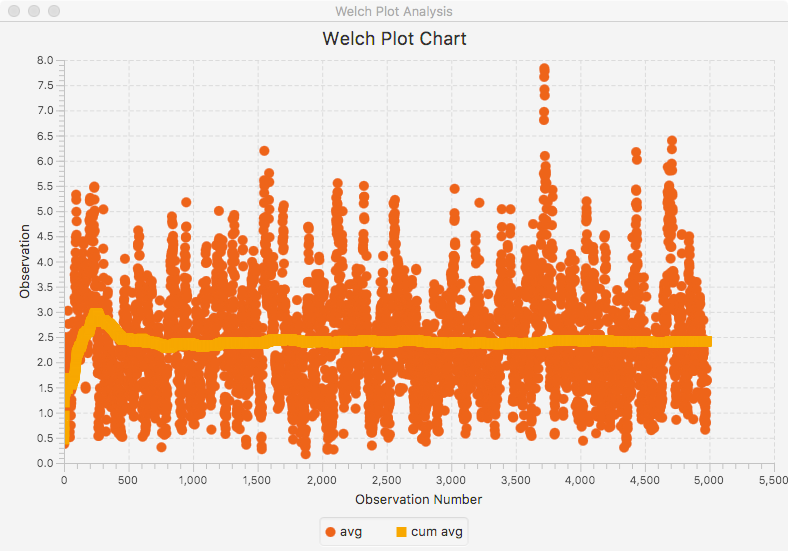
\includegraphics{./figures/ch7/WelchSysTimes.png}
\caption{\label{fig:WelchSysTimePlot}Welch Plot for System Time Analysis}
\end{figure}

Figure \ref{fig:WelchSysTimePlot} illustrates the plot of the
data. From this plot, we can estimate the number of observations
to delete as 2000.

Time-persistent observations are saved within a file from within the
model such that the time of the observation and the value of the state
variable at the time of change are recorded. Thus, the observations are
not equally spaced in time. In order to perform the Welch plot analysis,
we need to cut the data into discrete equally spaced intervals of time.

\begin{figure}
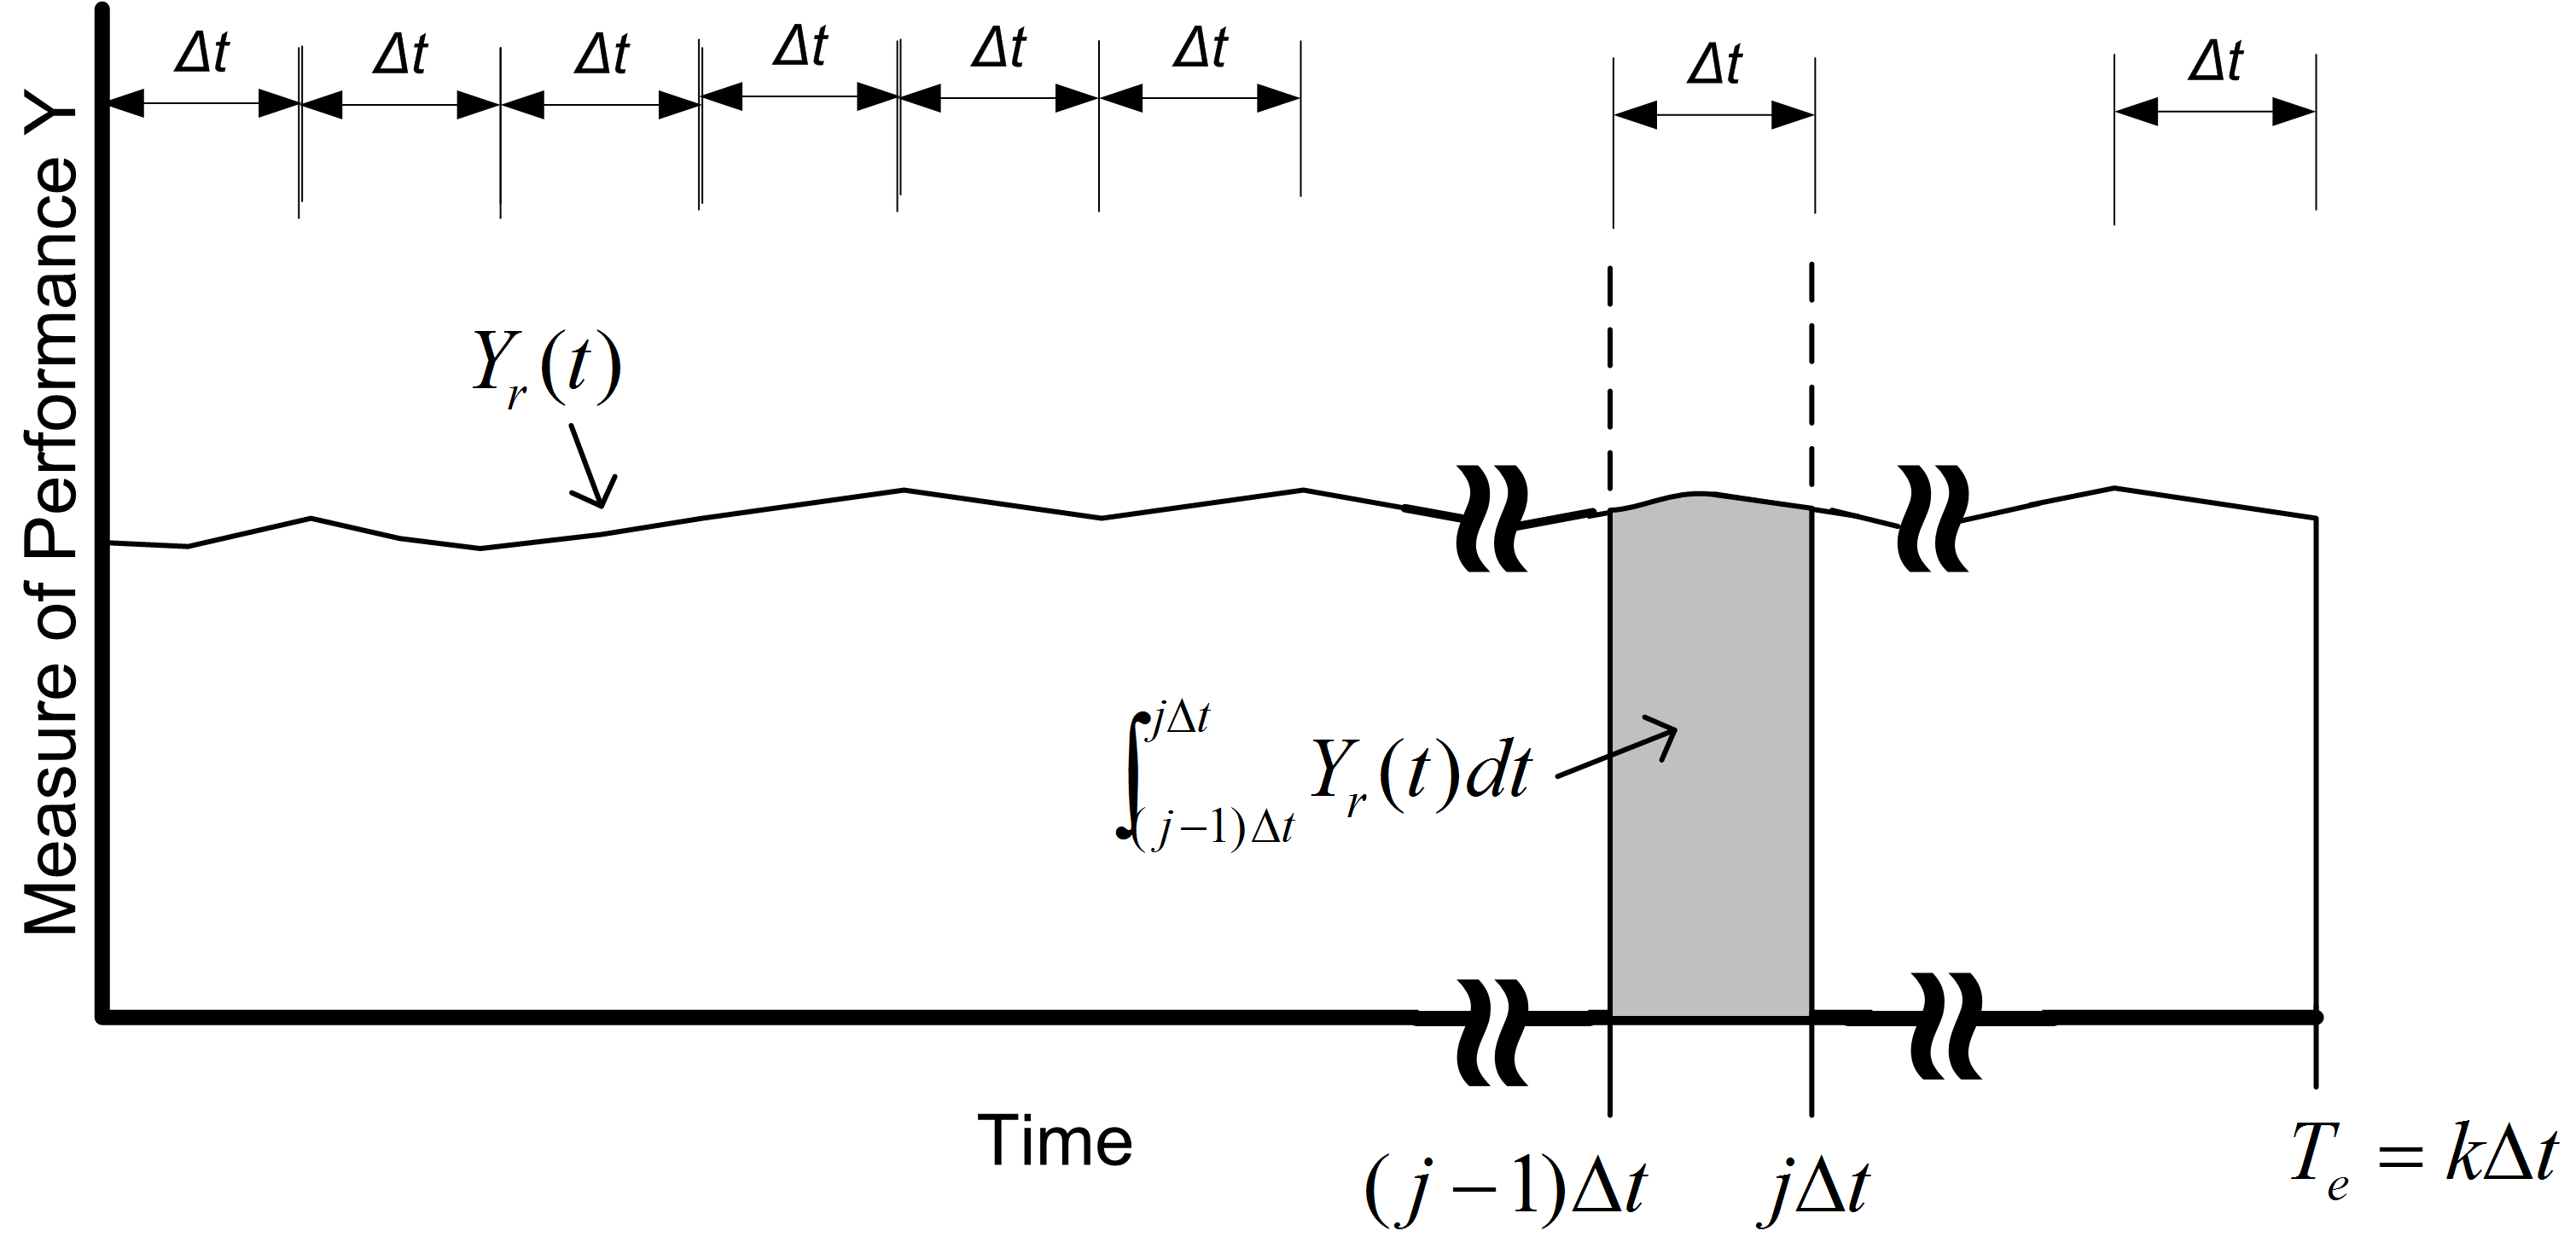
\includegraphics[width=0.8\linewidth,height=0.8\textheight]{./figures/ch7/ch7fig48} \caption{Discretizing Time-Persistent Data}\label{fig:DiscretizeTBD}
\end{figure}

Figure \ref{fig:DiscretizeTBD} illustrates the concept of discretizing time-persistent data. Suppose that you divide \(T_e\) into \(k\) intervals of size \(\Delta t\), so that \(T_e = k \times \Delta t\). The
time average over the \(j^{th}\) interval is given by:

\[\bar{Y}_{rj} = \dfrac{1}{\Delta t} \int_{j-1) \Delta t}^{j \Delta t} Y_r(t)dt\]

Thus, the overall time average can be computed from the time average
associated with each interval:

\[\begin{aligned}
\bar{Y}_{r} & = \dfrac{\int_0^{T_e} Y_r (t)dt}{T_e} =\dfrac{\int_0^{T_e} Y_r (t)dt}{k \Delta t} \\
& = \dfrac{\sum_{j=1}^{k}\int_{(j-1) \Delta t}^{j \Delta t} Y_r (t)dt}{k \Delta t} = \dfrac{\sum_{j=1}^{k} \bar{Y}_{rj}}{k}\end{aligned}\]

Each of the \(\bar{Y}_{rj}\) are computed over intervals of time that are
equally spaced and can be treated as if they are observation (tally)
based data.

The computation of the \(\bar{Y}_{rj}\) for time-persistent data can be
achieved by using the WelchDataFileCollectorTW class and specifying a
discretization interval. Since the number in queue data is
time-persistent, time based batches are selected, and the batch size is
specified in terms of time. In this case, the data is being batched
based on a time interval of 10 minutes in line~15 of the code listing. This produces a file which contains the \(\bar{Y}_{rj}\) as observations. This file can then be analyzed as
previously illustrated.

\begin{figure}
\centering
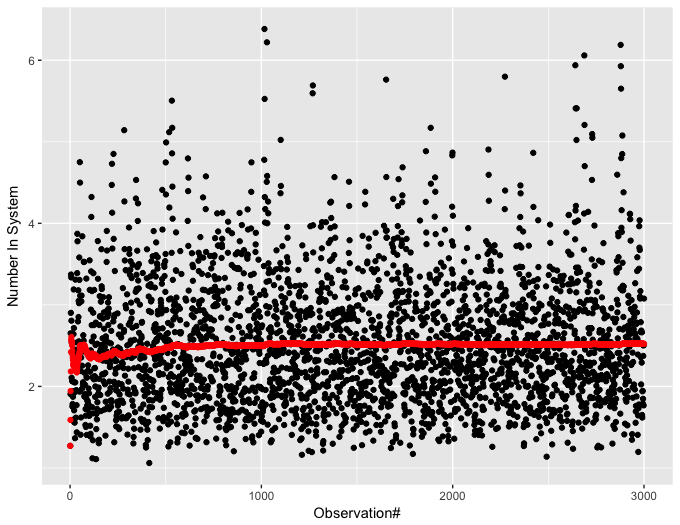
\includegraphics{./figures/ch7/NumInSysWelchPlot.png}
\caption{\label{fig:WPDiscretizeTBD}Welch Plot of Time-Persistent Number in System Data}
\end{figure}

The resulting plot is show in Figure \ref{fig:WPDiscretizeTBD}. This plot is sparser than the previous
plot because each observation represents the average of 10 minutes.
There are 3000 observations. From the plot, we can conclude that after
observation 1000, we see a steady convergence. The 1000th observation
represents 10000 time units (minutes) because every observation represents 10 time units.

Once you have performed the warm up analysis, you still need to use your
simulation model to estimate system performance. Because the process of
analyzing the warm up period involves saving the data you could use the
already saved data to estimate your system performance after truncating
the initial portion of the data from the data sets. If re-running the
simulation is relatively inexpensive, then you can simply set the warm
up period via the Simulation class and re-run the model. Following the
rule of thumb that the length of the run should be at least 10 times the
warm up period, the simulation was re-run with the settings (30
replications, 10000 minute warm up period, 100,000 minute replication
length). The results shown in the following table indicate that there does not appear to be
any significant bias with these replication settings.

\begin{longtable}[]{@{}lcc@{}}
\caption{Across Replication Statistics for Drive Through Pharmacy}\tabularnewline
\toprule
Response Name & \(\bar{x}\) & \(s\) \\
\midrule
\endfirsthead
\toprule
Response Name & \(\bar{x}\) & \(s\) \\
\midrule
\endhead
PharmacyQ:Num In Q & 1.637069 & 0.040491 \\
PharmacyQ:Time In Q & 1.636834 & 0.037817 \\
NumBusy & 0.700038 & 0.003435 \\
Number in System & 2.337107 & 0.043385 \\
System Time & 2.336790 & 0.039586 \\
Number of Replications & 30 & \\
\bottomrule
\end{longtable}

The true waiting time in the queue is \(1.6\bar{33}\) and it is clear that
the 95\% confidence interval contains this value.

The process described here for determining the warm up period for steady
state simulation is tedious and time consuming. Research into automating
this process is still an active area of investigation. The recent work
by \citep{robinson2005automated} and \citet{Rossetti:2005aa} holds some promise in
this regard; however, there remains the need to integrate these methods
into computer simulation software. Even though determining the warm up
period is tedious, some consideration of the warm up period should be
done for infinite horizon simulations.

Once the warm up period has been found, you can set the warm up period
using the Simulation class. Then, you can use the method of
replication-deletion to perform your simulation experiments. Thus, all
the discussion previously presented on the analysis of finite horizon
simulations can be applied.

When determining the number of replications, you can apply the fixed
sample size procedure after performing a pilot run. If the analysis
indicates that you need to make more runs to meet your confidence
interval half-width you have two alternatives: 1) increase the number of
replications or 2) keep the same number of replications but increase the
length of each replication. If \(n_0\) was the initial number of
replications and \(n\) is the number of replications recommended by the
sample size determination procedure, then you can instead set \(T_e\)
equal to \((n/n_0)T_e\) and run \(n_0\) replications. Thus, you will still
have approximately the same amount of data collected over your
replications, but the longer run length may reduce the effect of
initialization bias.

As previously mentioned, the method of replication-deletion causes each
replication to delete the initial portion of the run. As an alternative,
you can make one long run and delete the initial portion only once. When
analyzing an infinite horizon simulation based on one long replication,
a method is needed to address the correlation present in the within
replication data. The method of batch means is often used in this case
and has been automated in within the JSL. The next section discusses the
statistical basis for the batch means method and addresses some of the
practical issues of using it within the JSL.

\hypertarget{simoa:infhorizon:batchmeans}{%
\subsection{The Method of Batch Means}\label{simoa:infhorizon:batchmeans}}

In the batch mean method, only one simulation run is executed. After
deleting the warm up period, the remainder of the run is divided into
\(k\) batches, with each batch average representing a single observation.

\begin{figure}
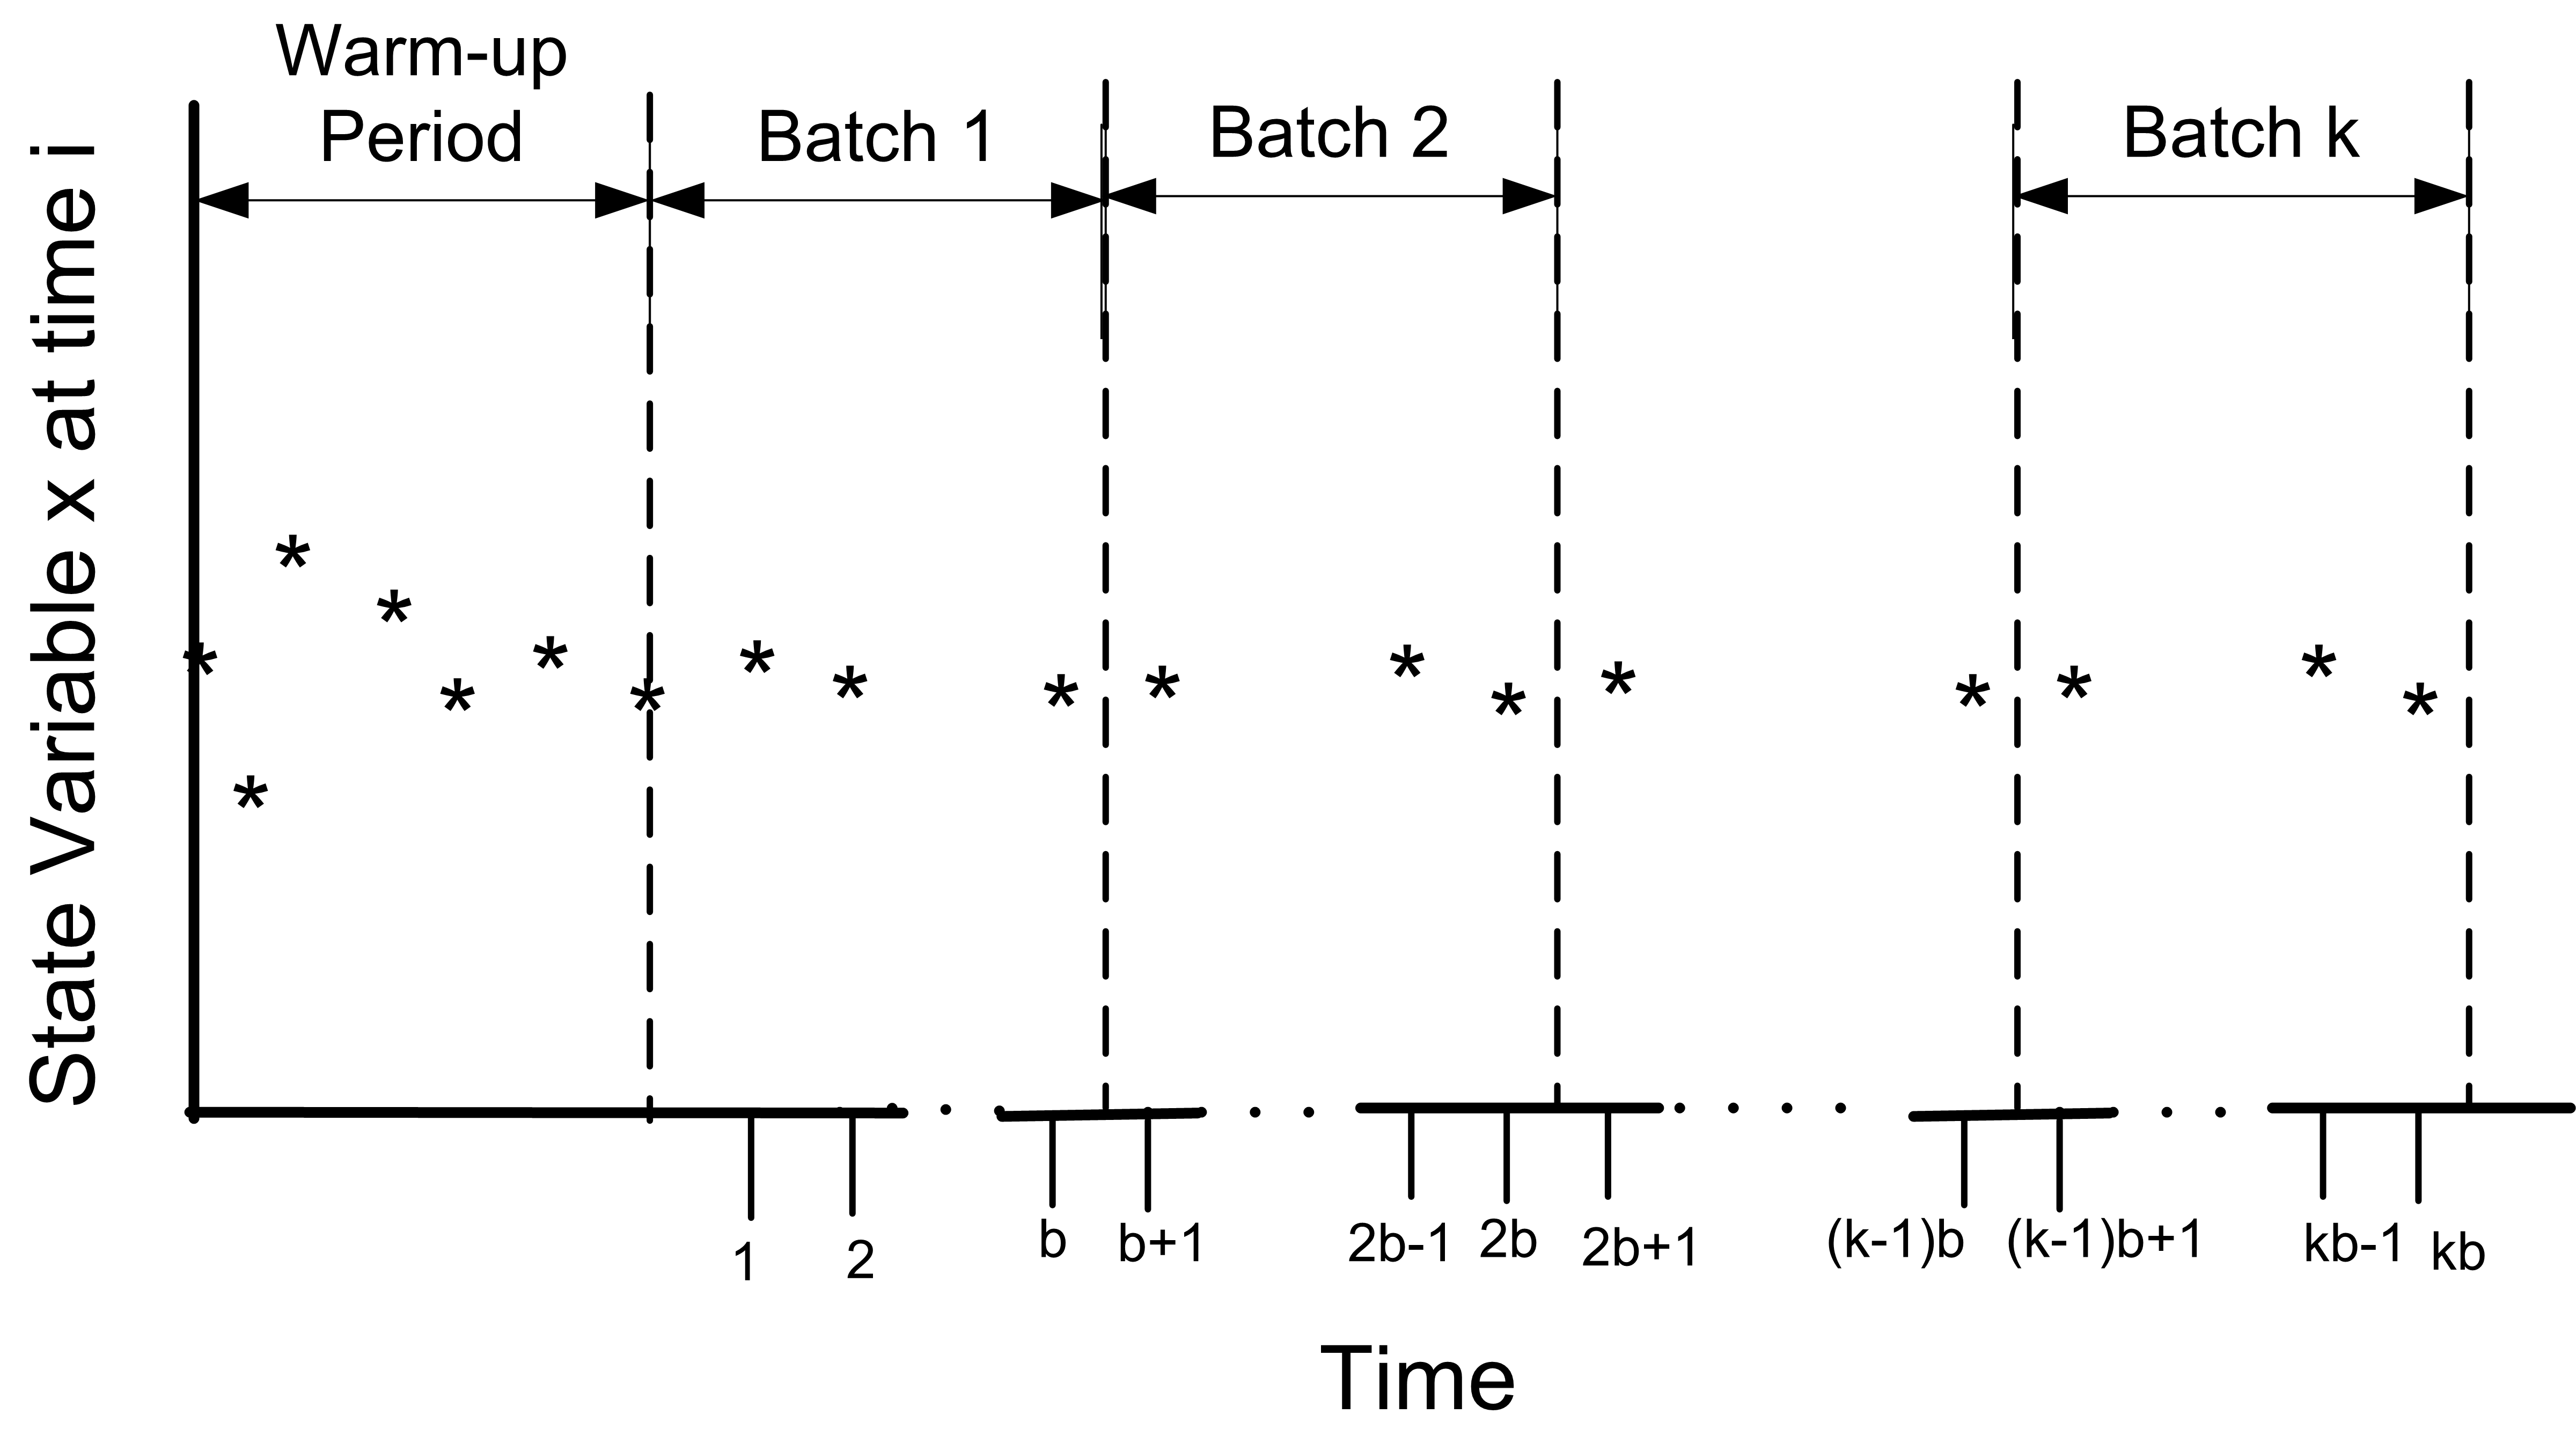
\includegraphics[width=0.8\linewidth,height=0.8\textheight]{./figures/ch7/ch7fig64} \caption{Illustration of the Batch MeansMethod}\label{fig:BatchMeans}
\end{figure}

Figure \ref{fig:BatchMeans} illustrates the concept of batching observations. The advantages of the batch means method are that it entails a long simulation run, thus dampening the effect of the initial conditions. The disadvantage is that the within replication data are correlated and
unless properly formed the batches may also exhibit a strong degree of correlation.

The following presentation assumes that a warm up analysis has already
been performed and that the data that has been collected occurs after
the warm up period. For simplicity, the presentation assumes observation
based data. The discussion also applies to time-based data that has been
cut into discrete equally spaced intervals of time as previously described.
Therefore, assume that a series of observations,
\((X_1, X_2, X_3, \ldots, X_n)\), is available from within the one long
replication after the warm up period. As shown earlier, the
within replication data can be highly correlated. In that section, it
was mentioned that standard confidence intervals based on

\[S^2(n) = \dfrac{1}{n - 1}\sum_{i=1}^n (X_i - \bar{X})^2\]

are not appropriate for this type of data. Suppose you were to ignore
the correlation, what would be the harm? In essence, a confidence
interval implies a certain level of confidence in the decisions based on
the confidence interval. When you use \(S^2(n)\) as defined above, you
will not achieve the desired level of confidence because \(S^2(n)\) is a
biased estimator for the variance of \(\bar{X}\) when the data are
correlated. Under the assumption that the data are covariance
stationary, an assessment of the harm in ignoring the correlation can be
made. For a series that is covariance stationary, one can show that

\[Var(\bar{X}) = \dfrac{\gamma_0}{n} \left[1 + 2 \sum_{k=1}^{n-1} \left(1 - \dfrac{k}{n} \right) \rho_k \right]\]

where \(\gamma_0 = Var(X_i)\), \(\gamma_k = Cov(X_i, X_{i + k})\), and
\(\rho_k = \gamma_k/\gamma_0\) for \(k = 1, 2, \ldots, n - 1\).

When the data are correlated, \(S^2/n\) is a biased estimator of
\(Var(\bar{X})\). To show this, you need to compute the expected value of
\(S^2/n\) as follows:

\[E\left[S^2/n\right] = \dfrac{\gamma_0}{n} \left[1 - \dfrac{2R}{n - 1}\right]\]

where

\[R = \sum_{k=1}^{n-1} (1 - \dfrac{k}{n}) \rho_k\]

Bias is defined as the difference between the expected value of the
estimator and the quantity being estimated. In this case, the bias can
be computed with some algebra as:

\[\text{Bias} = E\left[S^2/n\right] - Var(\bar{Y}) = \dfrac{-2 \gamma_0 R}{n - 1}\]

Since \(\gamma_0 > 0\) and \(n > 1\) the sign of the bias depends on the
quantity \emph{R} and thus on the correlation. There are three cases to
consider: zero correlation, negative correlation, and positive
correlation. Since \(-1 \leq \rho_k \leq 1\), examining the limiting
values for the correlation will determine the range of the bias.

For positive correlation, \(0 \leq \rho_k \leq 1\), the bias will be
negative, (\(- \gamma_0 \leq Bias \leq 0\)). Thus, the bias is negative if
the correlation is positive, and the bias is positive if the correlation
is negative. In the case of positive correlation, \(S^2/n\) underestimates
the \(Var(\bar{X})\). Thus, using \(S^2/n\) to form confidence intervals
will make the confidence intervals too short. You will have unjustified
confidence in the point estimate in this case. The true confidence will
not be the desired \(1 - \alpha\). Decisions based on positively
correlated data will have a higher than planned risk of making an error
based on the confidence interval.

One can easily show that for negative correlation,
\(-1 \leq \rho_k \leq 0\), the bias will be positive
(\(0 \leq Bias \leq \gamma_0\)). In the case of negatively correlated
data, \(S^2/n\) over estimates the \(Var(\bar{X})\). A confidence interval
based on \(S^2/n\) will be too wide and the true quality of the estimate
will be better than indicated. The true confidence coefficient will not
be the desired \(1 - \alpha\); it will be greater than \(1 - \alpha\).

Of the two cases, the positively correlated case is the more severe in
terms of its effect on the decision making process; however, both are
problems. Thus, the naive use of \(S^2/n\) for dependent data is highly
unwarranted. If you want to build confidence intervals on \(\bar{X}\) you
need to find an unbiased estimator of the \(Var(\bar{X})\).

The method of batch means provides a way to develop (at least
approximately) an unbiased estimator for \(Var(\bar{X})\). Assuming that
you have a series of data point, the method of batch means method
divides the data into subsequences of contiguous batches:

\[\begin{gathered}
\underbrace{X_1, X_2, \ldots, X_b}_{batch 1} \cdots
\underbrace{X_{b+1}, X_{b+2}, \ldots, X_{2b}}_{batch 2} \cdots \\
\underbrace{X_{(j-1)b+1}, X_{(j-1)b+2}, \ldots, X_{jb}}_{batch j}  \cdots
\underbrace{X_{(k-1)b+1}, X_{(k-1)b+2}, \ldots, X_{kb}}_{batch k}\end{gathered}\]

and computes the sample average of the batches. Let \(k\) be the number of
batches each consisting of \(b\) observations, so that
\(k = \lfloor n/b \rfloor\). If \(b\) is not a divisor of \(n\) then the last
\((n - kb)\) data points will not be used. Define \(\bar{X}_j(b)\) as the
\(j^{th}\) batch mean for \(j = 1, 2, \ldots, k\), where,

\[\bar{X}_j(b) = \dfrac{1}{b} \sum_{i=1}^b X_{(j-1)b+i}\]

Each of the batch means are treated like observations in the batch means
series. For example, if the batch means are re-labeled as
\(Y_j = \bar{X}_j(b)\), the batching process simply produces another
series of data, (\(Y_1, Y_2, Y_3, \ldots, Y_k\)) which may be more like a
random sample. To form a \(1 - \alpha\)\% confidence interval, you simply
treat this new series like a random sample and compute approximate
confidence intervals using the sample average and sample variance of the
batch means series:

\[\bar{Y}(k) = \dfrac{1}{k} \sum_{j=1}^k Y_j\]

\[S_b^2 (k) = \dfrac{1}{k - 1} \sum_{j=1}^k (Y_j - \bar{Y}^2)\]

\[\bar{Y}(k) \pm t_{\alpha/2, k-1} \dfrac{S_b (k)}{\sqrt{k}}\]

Since the original X's are covariance stationary, it follows that the
resulting batch means are also covariance stationary. One can show, see
\citep{alexopoulos1998output}, that the correlation in the batch means
reduces as both the size of the batches, \(b\) and the number of data
points, \(n\) increases. In addition, one can show that \(S_b^2 (k)/k\)
approximates \(\text{Var}(\bar{X})\) with error that reduces as both \(b\)
and \(n\) increase towards infinity.

The basic difficulty with the batch means method is determining the
batch size or alternatively the number of batches. Larger batch sizes
are good for independence but reduce the number of batches, resulting in
higher variance for the estimator. \citep{schmeiser1982batch} performed an
analysis that suggests that there is little benefit if the number of
batches is larger than 30 and recommended that the number of batches
remain in the range from 10 to 30. However, when trying to access
whether or not the batches are independent it is better to have a large
number of batches (\(>\) 100) so that tests on the lag-k correlation have
better statistical properties.

There are a variety of procedures that have been developed that will
automatically batch the data as it is collected, see for example
\citep{fishman1997an}, \citep{steiger2002an}, and \citet{banks2005discreteevent}. has its
own batching algorithm. The batching algorithm is described in
\citet{kelton2004simulation} page 311. See also \citep{fishman2001discreteevent}
page 254 for an analysis of the effectiveness of the algorithm.

The discussion here is based on the description in
\citet{kelton2004simulation}. When the algorithm has recorded a sufficient
amount of data, it begins by forming k = 20 batches. As more data is
collected, additional batches are formed until k = 40 batches are
collected. When 40 batches are formed, the algorithm collapses the
number of batches back to 20, by averaging each pair of batches. This
has the net effect of doubling the batch size. This process is repeated
as more data is collected, thereby ensuring that the number of batches
is between 20 and 39.

For time-persistent data, the approach requires that the data be
discretized as previously discussed in the section on warm up period
analysis. Then, the same batch method is applied to ensure between 20
and 39 batches. In addition, the process also computes the lag-1
correlation so that a test can be performed to check if the correlation
is significant by testing the hypothesis that the batch means are
uncorrelated using the following test statistic, see
\citep{alexopoulos1998output}:

\[C = \sqrt{\dfrac{k^2 - 1}{k - 2}}\biggl[ \hat{\rho}_1 + \dfrac{[Y_1 - \bar{Y}]^2 + [Y_k - \bar{Y}]^2}{2 \sum_{j=1}^k (Y_j - \bar{Y})^2}\biggr]\]

\[\hat{\rho}_1 = \dfrac{\sum_{j=1}^{k-1} (Y_j - \bar{Y})(Y_{j+1} - \bar{Y})}{\sum _{j=1}^k (Y_j - \bar{Y})^2}\]

The hypothesis is rejected if \(C > z_\alpha\) for a given confidence
level \(\alpha\). If the batch means do not pass the test, \emph{Correlated} is
reported for the half-width on the statistical reports.

\hypertarget{simoa:infhorizon:jslbatching}{%
\subsection{Performing the Method of Batch Means}\label{simoa:infhorizon:jslbatching}}

Performing the method of batch means in the JSL is relatively straight
forward. The following assumes that a warm up period analysis has
already been performed. Batches are formed during the simulation run and
the confidence intervals are based on the batches. In this situation,
the primary concern will be to determine the run length that will ensure
a desired half-width on the confidence intervals. Both fixed sampling
and sequential sampling methods can be applied.

The following code present the process to set up batching
within the JSL for the Drive Through Pharmacy Model. The key class is
the \texttt{StatisticalBatchingElement} class, which must be added to the \texttt{Model}
(see line~9) prior to running the simulation. Then, starting at line~20
the batch summary statistical reporting is captured. The
\texttt{StatisticalBatchingElement} has one key parameter which represents the
interval used to discretize the time weighted variables. If no interval
is supplied, then the algorithm ensures that the initial number of
batches collected before applying the previously described batching
algorithm is 512.

\begin{Shaded}
\begin{Highlighting}[]
\NormalTok{Simulation sim }\OperatorTok{=} \KeywordTok{new} \FunctionTok{Simulation}\OperatorTok{(}\StringTok{"Drive Through Pharmacy"}\OperatorTok{);}
\NormalTok{Model m }\OperatorTok{=}\NormalTok{ sim}\OperatorTok{.}\FunctionTok{getModel}\OperatorTok{();}
\CommentTok{// add DriveThroughPharmacy to the main model}
\NormalTok{DriveThroughPharmacy driveThroughPharmacy }\OperatorTok{=} \KeywordTok{new} \FunctionTok{DriveThroughPharmacy}\OperatorTok{(}\NormalTok{m}\OperatorTok{);}
\NormalTok{driveThroughPharmacy}\OperatorTok{.}\FunctionTok{setArrivalRS}\OperatorTok{(}\KeywordTok{new} \FunctionTok{ExponentialRV}\OperatorTok{(}\FloatTok{1.0}\OperatorTok{));}
\NormalTok{driveThroughPharmacy}\OperatorTok{.}\FunctionTok{setServiceRS}\OperatorTok{(}\KeywordTok{new} \FunctionTok{ExponentialRV}\OperatorTok{(}\FloatTok{0.7}\OperatorTok{));}

\CommentTok{// create the batching element for the simulation}
\NormalTok{StatisticalBatchingElement be }\OperatorTok{=} \KeywordTok{new} \FunctionTok{StatisticalBatchingElement}\OperatorTok{(}\NormalTok{m}\OperatorTok{);}

\CommentTok{// set the parameters of the experiment}
\NormalTok{sim}\OperatorTok{.}\FunctionTok{setNumberOfReplications}\OperatorTok{(}\DecValTok{1}\OperatorTok{);}
\NormalTok{sim}\OperatorTok{.}\FunctionTok{setLengthOfReplication}\OperatorTok{(}\FloatTok{1300000.0}\OperatorTok{);}
\NormalTok{sim}\OperatorTok{.}\FunctionTok{setLengthOfWarmUp}\OperatorTok{(}\FloatTok{100000.0}\OperatorTok{);}
\BuiltInTok{System}\OperatorTok{.}\FunctionTok{out}\OperatorTok{.}\FunctionTok{println}\OperatorTok{(}\StringTok{"Simulation started."}\OperatorTok{);}
\NormalTok{sim}\OperatorTok{.}\FunctionTok{run}\OperatorTok{();}
\BuiltInTok{System}\OperatorTok{.}\FunctionTok{out}\OperatorTok{.}\FunctionTok{println}\OperatorTok{(}\StringTok{"Simulation completed."}\OperatorTok{);}

\CommentTok{// get a StatisticReport from the batching element}
\NormalTok{StatisticReporter statisticReporter }\OperatorTok{=}\NormalTok{ be}\OperatorTok{.}\FunctionTok{getStatisticReporter}\OperatorTok{();}

\CommentTok{// print out the report}
\BuiltInTok{System}\OperatorTok{.}\FunctionTok{out}\OperatorTok{.}\FunctionTok{println}\OperatorTok{(}\NormalTok{statisticReporter}\OperatorTok{.}\FunctionTok{getHalfWidthSummaryReport}\OperatorTok{());}
\CommentTok{//System.out.println(be.asString());}

\CommentTok{// use the name of a response to get a reference to a particular response variable}
\NormalTok{ResponseVariable systemTime }\OperatorTok{=}\NormalTok{ m}\OperatorTok{.}\FunctionTok{getResponseVariable}\OperatorTok{(}\StringTok{"System Time"}\OperatorTok{);}
\CommentTok{// access the batch statistic from the batching element}
\NormalTok{BatchStatistic batchStatistic }\OperatorTok{=}\NormalTok{ be}\OperatorTok{.}\FunctionTok{getBatchStatistic}\OperatorTok{(}\NormalTok{systemTime}\OperatorTok{);}
\CommentTok{// get the actual batch mean values}
\DataTypeTok{double}\OperatorTok{[]}\NormalTok{ batchMeanArrayCopy }\OperatorTok{=}\NormalTok{ batchStatistic}\OperatorTok{.}\FunctionTok{getBatchMeanArrayCopy}\OperatorTok{();}
\BuiltInTok{System}\OperatorTok{.}\FunctionTok{out}\OperatorTok{.}\FunctionTok{println}\OperatorTok{(}\BuiltInTok{Arrays}\OperatorTok{.}\FunctionTok{toString}\OperatorTok{(}\NormalTok{batchMeanArrayCopy}\OperatorTok{));}
\end{Highlighting}
\end{Shaded}

The analysis performed to determine the warm up period should give you
some information concerning how long to make this single run and how
long to set it's warm up period. Assume that a warm up analysis has been
performed using \(n_0\) replications of length \(T_e\) and that the analysis
has indicated a warm up period of length \(T_w\). Then, we can use this
information is setting up the run length and warm up period for the
single replication experiment.

As previously discussed, the method of replication deletion spreads the
risk of choosing a bad initial condition across multiple replications.
The method of batch means relies on only one replication. If you were
satisfied with the warm up period analysis based on \(n_0\) replications
and you were going to perform replication deletion, then you are willing
to throw away the observations contained in at least \(n_0 \times T_w\)
time units and you are willing to use the data collected over
\(n_0 \times (T_e - T_w)\) time units. Therefore, the warm up period for
the single replication can be set at \(n_0 \times T_w\) and the run length
can be set at \(n_0 \times T_e\). For example, suppose your warm up
analysis was based on the initial results of \(n_0\) = 10, \(T_e\) = 30000,
\(T_w\) = 10000. Thus, your starting run length would be
\(n_0 \times T_e = 10 \times 30,000 = 300,000\) and the warm period will
be \(n_0 \times T_w = 100,000\). The following table show the results based on replication deletion

\begin{longtable}[]{@{}lccc@{}}
\caption{Replication-Deletion Half-Width Summary report \(n=10\), \(T_e = 30000\), \(T_w = 10000\)}\tabularnewline
\toprule
Response Name & \(n\) & \(\bar{x}\) & \(hw\) \\
\midrule
\endfirsthead
\toprule
Response Name & \(n\) & \(\bar{x}\) & \(hw\) \\
\midrule
\endhead
PharmacyQ:Num In Q & 10 & 1.656893 & 0.084475 \\
PharmacyQ:Time In Q & 10 & 1.659100 & 0.082517 \\
NumBusy & 10 & 0.699705 & 0.004851 \\
Num in System & 10 & 2.356598 & 0.088234 \\
System Time & 10 & 2.359899 & 0.085361 \\
\bottomrule
\end{longtable}

This table shows the results based on batching one long replication.

\begin{longtable}[]{@{}lccc@{}}
\caption{Batch Means Summary Report \(T_e = 300000\), \(T_w = 100000\)}\tabularnewline
\toprule
Response Name & \(n\) & \(\bar{x}\) & \(hw\) \\
\midrule
\endfirsthead
\toprule
Response Name & \(n\) & \(\bar{x}\) & \(hw\) \\
\midrule
\endhead
PharmacyQ:Num In Q & 32 & 1.631132 & 0.047416 \\
PharmacyQ:Time In Q & 24 & 1.627059 & 0.055888 \\
NumBusy & 32 & 0.699278 & 0.004185 \\
Num in System & 32 & 2.330410 & 0.049853 \\
System Time & 24 & 2.324590 & 0.057446 \\
\bottomrule
\end{longtable}

Suppose now you want to ensure that the half-widths from a single
replication are less than a given error bound. The half-widths reported
by the simulation for a single replication are based on the \emph{batch
means}. You can get an approximate idea of how much to increase the
length of the replication by using the half-width sample size
determination formula.

\[n \cong n_0 \left(\dfrac{h_0}{h}\right)^2\]

In this case, you interpret \(n\) and \(n_0\) as the number of batches. From
previous results, there were 32 batches for the time-weighted
variables. Based on \(T_e = 300000\) and \(T_w = 100000\) there was a total
of \(T_e - T_w = 200000\) time units of observed data. This means that
each batch represents \(200,000\div 32 = 6250\) time units. Using this
information in the half-width based sample size formula with \(n_0 = 32\),
\(h_0 = 0.049\), and \(h = 0.02\), for the number in the system, yields:

\[n \cong n_0 \dfrac{h_0^2}{h^2} = 32 \times \dfrac{(0.049)^2}{(0.02)^2} = 192 \ \ \text{batches}\]

Since each batch in the run had 6250 time units, this yields the need
for 1,200,000 time units of observations. Because of the warm up period,
you therefore need to set \(T_e\) equal to (1,200,000 + 100,000 =
1,300,000). Re-running the simulation yields the results shown in
the following table. The results show that the half-width meets
the desired criteria. This approach is approximate since you do not know
how the observations will be batched when making the final run.

\begin{longtable}[]{@{}lccc@{}}
\caption{Batch Means Summary Report \(T_e = 1,300,000\), \(T_w = 100000\)}\tabularnewline
\toprule
Response Name & \(n\) & \(\bar{x}\) & \(hw\) \\
\midrule
\endfirsthead
\toprule
Response Name & \(n\) & \(\bar{x}\) & \(hw\) \\
\midrule
\endhead
NumBusy & 32 & 0.698973 & 0.001652 \\
Num in System & 32 & 2.322050 & 0.019413 \\
PharmacyQ:Num In Q & 32 & 1.623077 & 0.018586 \\
PharmacyQ:Time In Q & 36 & 1.625395 & 0.017383 \\
System Time & 36 & 2.324915 & 0.017815 \\
\bottomrule
\end{longtable}

Rather than trying to fix the amount of sampling, you might instead try
to use a sequential sampling technique that is based on the half-width
computed during the simulation run. In order to do this, we need to
create a specific observer that can stop the simulation when the
half-width criteria is met. Currently, the JSL does not facilitate this approach.

Once the warm up period has been analyzed, performing infinite horizon
simulations using the batch means method is relatively straight forward.
A disadvantage of the batch means method is that it will be more
difficult to use the statistical classical experimental design methods.
If you are faced with an infinite horizon simulation, then you can use
either the replication-deletion approach or the batch means method
readily within the JSL. In either case, you should investigate if there
may be any problems related to initialization bias. If you use the
replication-deletion approach, you should play it safe when specifying
the warm up period. Making the warm up period longer than you think it
should be is better than replicating a poor choice. When performing an
infinite horizon simulation based on one long run, you should make sure
that your run length is long enough. A long run length can help to ``wash
out'' the effects of initial condition bias.

Ideally, in the situation where you have to make many simulation
experiments using different parameter settings of the same model, you
should perform a warm up analysis for each design configuration. In
practice, this is not readily feasible when there are a large number of
experiments. In this situation, you should use your common sense to pick
the design configurations (and performance measures) that you feel will
most likely suffer from initialization bias. If you can determine long
enough warm up periods for these configurations, the other
configurations should be relatively safe from the problem by using the
longest warm up period found.

There are a number of other techniques that have been developed for the
analysis of infinite horizon simulations including the standardized time
series method, the regenerative method, and spectral methods. An
overview of these methods and others can be found in
\citep{alexopoulos1998output} and in \citep{law2007simulation}.

So far you have learned how to analyze the data from one design
configuration. A key use of simulation is to be able to compare
alternative system configurations and to assist in choosing which
configurations are best according to the decision criteria. The next
section discusses how to compare different system configurations.

\hypertarget{simoa:comparingSystems}{%
\section{Comparing System Configurations}\label{simoa:comparingSystems}}

The previous sections have concentrated on estimating the performance of
a system through the execution of a single simulation model. The running
of the model requires the specification of the input variables (e.g.
mean time between arrivals, service distribution, etc.) and the
structure of the model (e.g.~FIFO queue, process flow, etc.) The
specification of a set of inputs (variables and/or structure) represents
a particular system configuration, which is then simulated to estimate
performance. To be able to simulate design configurations, you may have
to build different models or you may be able to use the same model
supplied with different values of the program inputs. In either
situation, you now have different design configurations that can be
compared. This allows the performance of the system to be estimated
under a wide-variety of controlled conditions. It is this ability to
easily perform these what-if simulations that make simulation such a
useful analysis tool.

Naturally, when you have different design configurations, you would like
to know which configurations are better than the others. Since the
simulations are driven by random variables, the outputs from each
configuration (e.g.~\(Y^1, Y^2\)) are also random variables. The estimate
of the performance of each system must be analyzed using statistical
methods to ensure that the differences in performance are not simply due
to sampling error. In other words, you want to be confident that one
system is statistically better (or worse) than the other system.

\hypertarget{simoa:comparingSystems:two}{%
\subsection{Comparing Two Systems}\label{simoa:comparingSystems:two}}

The techniques for comparing two systems via simulation are essentially
the same as that found in books that cover the statistical analysis of
two samples (e.g. \citep{montgomery2006applied}). This section begins with a
review of these methods. Assume that samples from two different
populations (system configurations) are available:

\[X_{11}, X_{12},\ldots, X_{1 n_1} \ \ \text{a sample of size $n_1$ from system configuration 1}\]

\[X_{21}, X_{22},\ldots, X_{2 n_2} \ \ \text{a sample of size $n_2$ from system configuration 2}\]

The samples represent a performance measure of the system that will be
used in a decision regarding which system configuration is preferred.
For example, the performance measure may be the average system
throughput per day, and you want to pick the design configuration that
has highest throughput.

Assume that each system configuration has an unknown population mean for
the performance measure of interest, \(E[X_1] = \theta_1\) and
\(E[X_2] = \theta_2\). Thus, the problem is to determine, with some
statistical confidence, whether \(\theta_1 < \theta_2\) or alternatively
\(\theta_1 > \theta_2\). Since the system configurations are different, an
analysis of the situation of whether \(\theta_1 = \theta_2\) is of less
relevance in this context.

Define \(\theta = \theta_1 - \theta_2\) as the mean difference in
performance between the two systems. Clearly, if you can determine
whether \(\theta >\) 0 or \(\theta <\) 0 you can determine whether
\(\theta_1 < \theta_2\) or \(\theta_1 > \theta_2\). Thus, it is sufficient
to concentrate on the difference in performance between the two systems.

Given samples from two different populations, there are a number of ways
in which the analysis can proceed based on different assumptions
concerning the samples. The first common assumption is that the
observations within each sample for each configuration form a random
sample. That is, the samples represent independent and identically
distributed random variables. Within the context of simulation, this can
be easily achieved for a given system configuration by performing
replications. For example, this means that
\(X_{11}, X_{12},\ldots, X_{1 n_1}\) are the observations from \(n_1\)
replications of the first system configuration. A second common
assumption is that both populations are normally distributed or that the
central limit theorem can be used so that sample averages are at least
approximately normal.

To proceed with further analysis, assumptions concerning the population
variances must be made. Many statistics textbooks present results for
the case of the population variance being known. In general, this is not
the case within simulation contexts, so the assumption here will be that
the variances associated with the two populations are unknown. Textbooks
also present cases where it is assumed that the population variances are
equal. Rather than making that assumption it is better to test a
hypothesis regarding equality of population variances.

The last assumption concerns whether or not the two samples can be
considered independent of each other. This last assumption is very
important within the context of simulation. Unless you take specific
actions to ensure that the samples will be independent, they will, in
fact, be dependent because of how simulations use (re-use) the same
random number streams. The possible dependence between the two samples
is not necessarily a bad thing. In fact, under certain circumstance it
can be a good thing.

The following sections first presents the methods for analyzing the case
of unknown variance with independent samples. Then, we focus on the case
of dependence between the samples. Finally, how to use the JSL to do the
work of the analysis will be illustrated.

\hypertarget{simoa:comparingSystems:twoIND}{%
\subsubsection{Analyzing Two Independent Samples}\label{simoa:comparingSystems:twoIND}}

Although the variances are unknown, the unknown variances are either
equal or not equal. In the situation where the variances are equal, the
observations can be pooled when developing an estimate for the variance.
In fact, rather than just assuming equal or not equal variances, you can
(and should) use an F-test to test for the equality of variance. The
F-test can be found in most elementary probability and statistics books
(see \citep{montgomery2006applied}).

The decision regarding whether \(\theta_1 < \theta_2\) can be addressed by
forming confidence intervals on \(\theta = \theta_1 - \theta_2\). Let
\(\bar{X}_1\), \(\bar{X}_2\), \(S_1^2\), and \(S_2^2\) be the sample averages
and sample variances based on the two samples (k = 1,2):

\[\bar{X}_k = \dfrac{1}{n_k} \sum_{j=1}^{n_k} X_{kj}\]

\[S_k^2 = \dfrac{1}{n_k - 1} \sum_{j=1}^{n_k} (X_{kj} - \bar{X}_k)^2\]

An estimate of \(\theta = \theta_1 - \theta_2\) is desired. This can be
achieved by estimating the difference with
\(\hat{D} = \bar{X}_1 - \bar{X}_2\). To form confidence intervals on
\(\hat{D} = \bar{X}_1 - \bar{X}_2\) an estimator for the variance of
\(\hat{D} = \bar{X}_1 - \bar{X}_2\) is required. Because the samples are
independent, the computation of the variance of the difference is:

\[Var(\hat{D}) = Var(\bar{X}_1 - \bar{X}_2) = \dfrac{\sigma_1^2}{n_1} + \dfrac{\sigma_2^2}{n_2}\]

where \(\sigma_1^2\) and \(\sigma_2^2\) are the unknown population
variances. Under the assumption of equal variance,
\(\sigma_1^2 = \sigma_2^2 =\sigma^2\), this can be written as:

\[Var(\hat{D}) = Var(\bar{X}_1 - \bar{X}_2) = \dfrac{\sigma_1^2}{n_1} + \dfrac{\sigma_2^2}{n_2} = \sigma^2 (\dfrac{1}{n_1} + \dfrac{1}{n_2})\]

where \(\sigma^2\) is the common unknown variance. A pooled estimator of
\(\sigma^2\) can be defined as:

\[S_p^2 = \dfrac{(n_1 - 1)S_1^2 + (n_2 - 1)S_2^2}{n_1 + n_2 - 2}\]

Thus, a (\(1 - \alpha\))\% confidence interval on
\(\theta = \theta_1 - \theta_2\) is:

\[\hat{D} \pm t_{\alpha/2 , v} s_p \sqrt{\dfrac{1}{n_1} + \dfrac{1}{n_2}}\]

where \(v = n_1 + n_2 - 2\). For the case of unequal variances, an
approximate (\(1 - \alpha\))\% confidence interval on
\(\theta = \theta_1 - \theta_2\) is given by:

\[\hat{D} \pm t_{\alpha/2 , v} \sqrt{S_1^2/n_1 + S_2^2/n_2}\]

where
\[v = \Biggl\lfloor \frac{(S_1^2/n_1 + S_2^2/n_2)^2}{\frac{(S_1^2/n_1)^2}{n_1 +1} + \frac{(S_2^2/n_2)^2}{n_2 + 1}} - 2 \Biggr\rfloor\]

Let \([l, u]\) be the resulting confidence interval where \(l\) and \(u\)
represent the lower and upper limits of the interval with by
construction \(l < u\). Thus, if \(u < 0\), you can conclude with
(\(1 - \alpha\))\% confidence that \(\theta = \theta_1 - \theta_2 < 0\) (i.e.
that \(\theta_1 < \theta_2\)). If \(l > 0\), you can conclude with
(\(1 - \alpha\))\% that \(\theta = \theta_1 - \theta_2 > 0\) (i.e.~that
\(\theta_1 > \theta_2\)). If \([l, u]\) contains 0, then no conclusion can
be made at the given sample sizes about which system is better. This
does not indicate that the system performance is the same for the two
systems. You \emph{know} that the systems are different. Thus, their
performance will be different. This only indicates that you have not
taken enough samples to detect the true difference. If sampling is
relatively cheap, then you may want to take additional samples in order
to discern an ordering between the systems.

Two configurations are under consideration for the design of an airport
security checkpoint. A simulation model of each design was made. The
replication values of the throughput per minute for the security station
for each design are provided in the following table.

\begin{longtable}[]{@{}lcc@{}}
\toprule
& Design 1 & Design 2 \\
\midrule
\endhead
1 & 10.98 & 8.93 \\
2 & 8.87 & 9.82 \\
3 & 10.53 & 9.27 \\
4 & 9.40 & 8.50 \\
5 & 10.10 & 9.63 \\
6 & 10.28 & 9.55 \\
7 & 8.86 & 9.30 \\
8 & 9.00 & 9.31 \\
9 & 9.99 & 9.23 \\
10 & 9.57 & 8.88 \\
11 & & 8.05 \\
12 & & 8.74 \\
\(\bar{x}\) & 9.76 & 9.10 \\
\(s\) & 0.74 & 0.50 \\
\(n\) & 10 & 12 \\
\bottomrule
\end{longtable}

Assume that the two simulations were run independently of each other,
using different random numbers. Recommend the better design with 95\%
confidence.

According to the results:

\[\hat{D} = \bar{X}_1 - \bar{X}_2 = 9.76 - 9.1 = 0.66\]

In addition, we should test if the variances of the samples are equal.
This requires an \(F\) test, with \(H_0: \sigma_{1}^{2} = \sigma_{2}^{2}\)
versus \(H_1: \sigma_{1}^{2} \neq \sigma_{2}^{2}\). Based on elementary
statistics, the test statistic is: \(F_0 = S_{1}^{2}/S_{1}^{2}\). The
rejection criterion is to reject \(H_0\) if
\(F_0 > f_{\alpha/2, n_1-1, n_2 -1}\) or
\(F_0 < f_{1-\alpha/2, n_1-1, n_2 -1}\), where \(f_{p, u, v}\) is the upper
percentage point of the \(F\) distribution. Assuming a 0.01 significance
level for the \(F\) test, we have \(F_0 = (0.74)^{2}/(0.50)^{2} = 2.12\).
Since \(f_{0.005, 9, 11} = 5.54\) and \(f_{0.995, 9, 11} = 0.168\), there is
not enough evidence to conclude that the variances are different at the
0.01 significance level. The value of \(f_{p, u, v}\) can be determined in
as F.INV.RT(p, u, v). Note also that \(f_{1-p, u, v} = 1/f_{p, v, u}\). In
\(R\), the formula is \(f_{p, u, v} = qt(1-p, u,v)\), since \(R\) provides the
quantile function, not the upper right tail function.

Since the variances can be assumed equal, we can use the pooled
variance, which is:

\[\begin{aligned}
S_p^2 & = \dfrac{(n_1 - 1)S_1^2 + (n_2 - 1)S_2^2}{n_1 + n_2 - 2}\\
  & = \dfrac{(10 - 1)(0.74)^2 + (12 - 1)(0.5)^2}{12 + 10 - 2} \\
  & = 0.384\end{aligned}\]

Thus, a (\(1 -0.05\))\% confidence interval on
\(\theta = \theta_1 - \theta_2\) is:

\[\begin{aligned}
\hat{D} & \pm t_{\alpha/2 , v} s_p \sqrt{\dfrac{1}{n_1} + \dfrac{1}{n_2}} \\
0.66 &  \pm t_{0.025 , 20} (\sqrt{0.384}) \sqrt{\dfrac{1}{10} + \dfrac{1}{12}} \\
0.66 & \pm (2.086)(0.6196)(0.428) \\
0.66 & \pm 0.553\end{aligned}\]

where \(v = n_1 + n_2 - 2 = 10 + 12 - 2 = 20\). Since this results in an
interval \([0.10, 1.21]\) that does not contain zero, we can conclude that
design 1 has the higher throughput with 95\% confidence.

The confidence interval can assist in making decisions regarding
relative performance of the systems from a \emph{statistically significant}
standpoint. However, if you make a conclusion about the ordering of the
system, it still may not be practically significant. That is, the
difference in the system performance is statistically significant but
the actual difference is of no practical use. For example, suppose you
compare two systems in terms of throughput with resulting output
\(\bar{X}_1\) = 5.2 and \(\bar{X}_2\) = 5.0 with the difference
statistically significant. While the difference of 0.2 may be
statistically significant, you might not be able to achieve this in the
actual system. After all, you are making a decision based on a \emph{model of
the system} not on the real system. If the costs of the two systems are
significantly different, you should prefer the cheaper of the two
systems since there is no practical difference between the two systems.
The fidelity of the difference is dependent on your modeling
assumptions. Other modeling assumptions may overshadow such a small
difference.

The notion of practical significance is model and performance measure
dependent. One way to characterize the notion of practical significance
is to conceptualize a zone of performance for which you are indifferent
between the two systems.

\begin{figure}
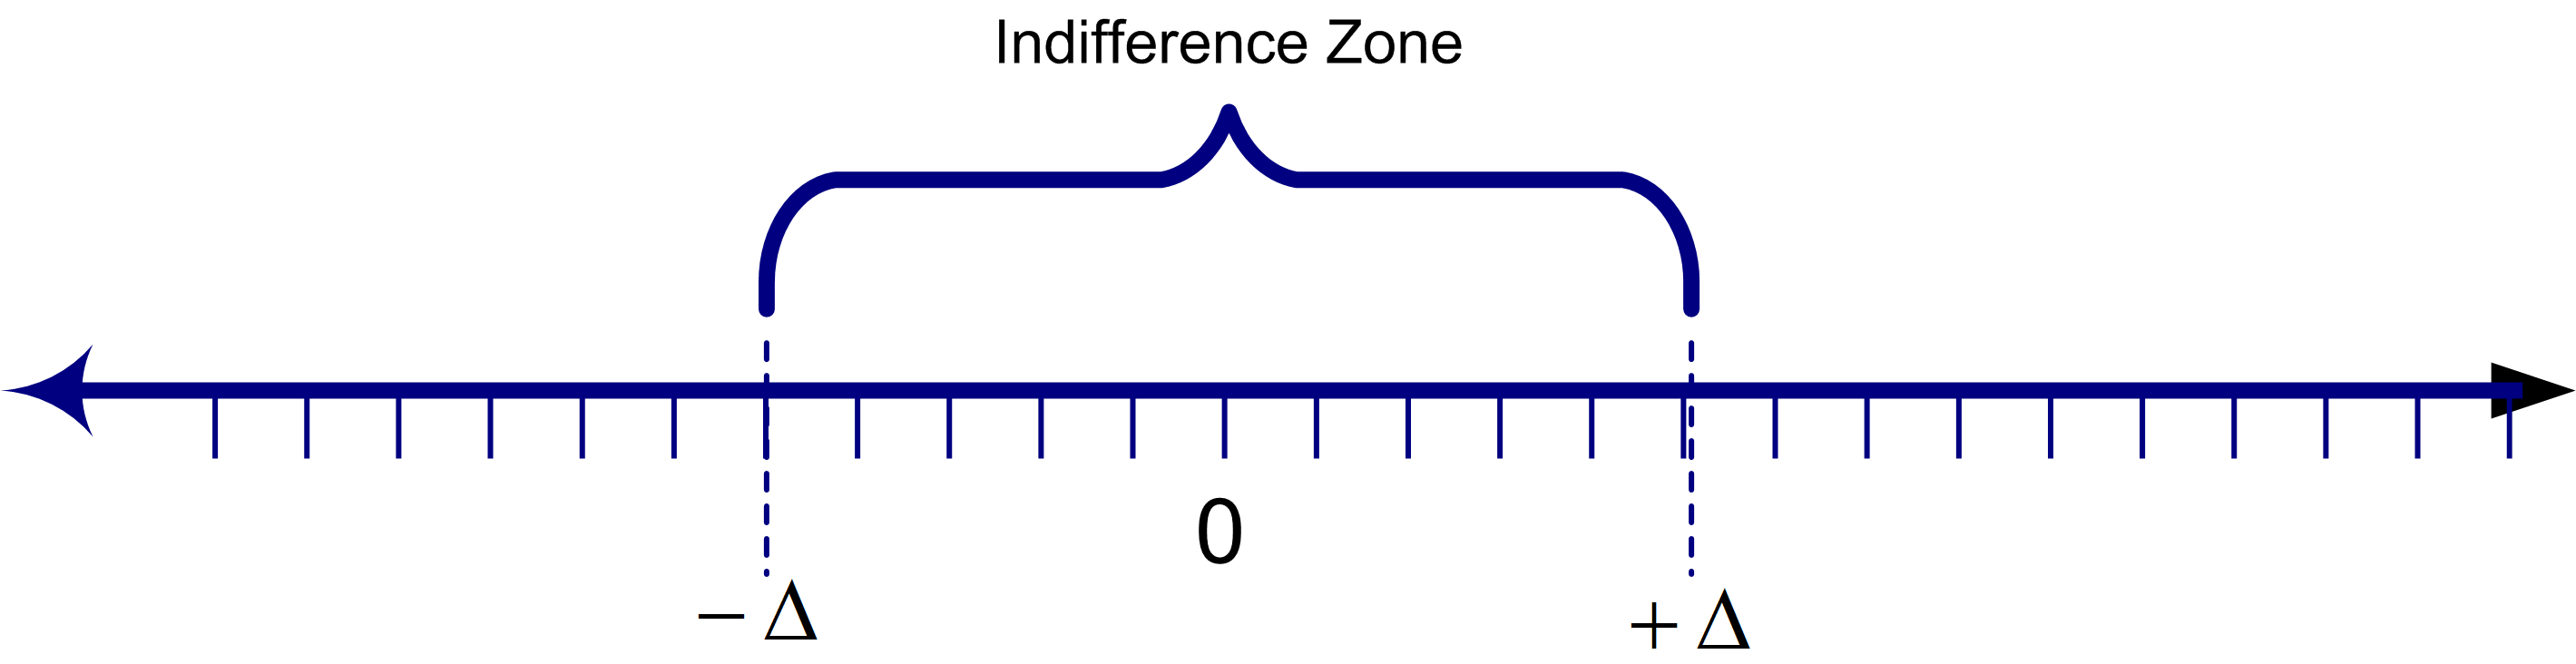
\includegraphics[width=0.8\linewidth,height=0.8\textheight]{./figures/ch7/ch7fig72} \caption{Indifference Zone Concept}\label{fig:IndifZone}
\end{figure}

Figure \ref{fig:IndifZone} illustrates the concept of an indifference zone
around the difference between the two systems. If the difference between
the two systems falls in this zone, you are indifferent between the two
systems (i.e.~there is no practical difference).

Using the indifference zone to model the notion of practical
significance, if \(u < -\Delta\), you can conclude confidence that
\(\theta_1 < \theta_2\), and if \(l > \Delta\), you can conclude with
confidence that \(\theta_1 > \theta_2\). If \(l\) falls within the
indifference zone and \(u\) does not (or vice versa), then there is not
enough evidence to make a confident conclusion. If \([l,u]\) is totally
contained within the indifference zone, then you can conclude with
confidence that there is no practical difference between the two
systems.

\hypertarget{simoa:comparingSystems:twoDep}{%
\subsubsection{Analyzing Two Dependent Samples}\label{simoa:comparingSystems:twoDep}}

In this situation, continue to assume that the observations within a
sample are independent and identically distributed random variables;
however, the samples themselves are not independent. That is, assume
that the \((X_{11}, X_{12},\ldots, X_{1n_1})\) and \((X_{21}, X_{22}, \ldots, X_{2n_2})\) from the
two systems are dependent.

For simplicity, suppose that the difference in the configurations can be
implemented using a simple parameter change within the model. For
example, the mean processing time is different for the two
configurations. First, run the model to produce
\((X_{11}, X_{12}, \ldots, X_{1n_1})\) for configuration 1. Then, change
the parameter and re-executed the model to produce
\((X_{21}, X_{22}, \ldots, X_{2n_2})\) for configuration 2.

Assuming that you did nothing with respect to the random number streams,
the second configuration used the same random numbers that the first
configuration used. Thus, the generated responses will be correlated
(dependent). In this situation, it is convenient to assume that each
system is run for the same number of replications, i.e.~\(n_1\) = \(n_2\) =
n.~Since each replication for the two systems uses the same random
number streams, the correlation between \((X_{1,j}, X_{2,j})\) will not be
zero; however, each pair will still be independent \emph{across} the
replications. The basic approach to analyzing this situation is to
compute the difference for each pair:

\[D_j = X_{1j} - X_{2j} \ \ \text{for} \; j = 1,2,\ldots,n\]

The \((D_1, D_2, \ldots, D_n)\) will form a random sample, which can be
analyzed via traditional methods. Thus, a (\(1 - \alpha\))\% confidence
interval on \(\theta = \theta_1 - \theta_2\) is:

\[\bar{D} = \dfrac{1}{n} \sum_{j=1}^n D_j\]

\[S_D^2 = \dfrac{1}{n-1} \sum_{j=1}^n (D_j - \bar{D})^2\]

\[\bar{D} \pm t_{\alpha/2, n-1} \dfrac{S_D}{\sqrt{n}}\]

The interpretation of the resulting confidence interval \([l, u]\) is the
same as in the independent sample approach. This is the paired-t
confidence interval presented in statistics textbooks.

Assume that the two simulations were run dependently using common random
numbers. Recommend the better design with 95\% confidence.

According to the results:

\[\bar{D} = \bar{X}_1 - \bar{X}_2 = 50.88 - 48.66 = 2.22\]

Also, we have that \(S_D^2 = (0.55)^2\). Thus, a (\(1 -0.05\))\% confidence
interval on \(\theta = \theta_1 - \theta_2\) is:

\[\begin{aligned}
\hat{D} & \pm t_{\alpha/2, n-1} \dfrac{S_D}{\sqrt{n}}\\
2.22 &  \pm t_{0.025 , 9}  \dfrac{0.55}{\sqrt{10}}\\
2.22 & \pm (2.261)(0.1739)\\
2.22 & \pm 0.0.393\end{aligned}\]

Since this results in an interval \([1.827, 2.613]\) that does not contain
zero, we can conclude that design 1 has the higher cost with 95\%
confidence.

Of the two approaches (independent versus dependent) samples, the latter
is much more prevalent in simulation contexts. The approach is called
the method of \emph{common random numbers (CRN)} and is a natural by product
of how most simulation languages handle their assignment of random
number streams.

To understand why this method is the preferred method for comparing two
systems, you need to understand the method's affect on the variance of
the estimator. In the case of independent samples, the estimator of
performance was \(\hat{D} = \bar{X}_1 - \bar{X}_2\). Since

\[\begin{aligned}
\bar{D} & = \dfrac{1}{n} \sum_{j=1}^n D_j \\
 & =  \dfrac{1}{n} \sum_{j=1}^n (X_{1j} - X_{2j}) \\
 & = \dfrac{1}{n} \sum_{j=1}^n X_{1j} - \dfrac{1}{n} \sum_{j=1}^n X_{2j} \\
 & = \bar{X}_1 - \bar{X}_2 \\
 & = \hat{D}\end{aligned}\]

The two estimators are the same, when \(n_1 = n_2 = n\); however, their
variances are not the same. Under the assumption of independence,
computing the variance of the estimator yields:

\[V_{\text{IND}} = Var(\bar{X}_1 - \bar{X}_2) = \dfrac{\sigma_1^2}{n} + \dfrac{\sigma_2^2}{n}\]

Under the assumption that the samples are not independent, the variance
of the estimator is:

\[V_{\text{CRN}} = Var(\bar{X}_1 - \bar{X}_2) = \dfrac{\sigma_1^2}{n} + \dfrac{\sigma_2^2}{n} - 2\text{cov}(\bar{X}_1, \bar{X}_2)\]

If you define \(\rho_{12} = corr(\bar{X}_1, \bar{X}_2)\), the variance for
the common random number situation is:

\[V_{\text{CRN}} = V_{\text{IND}} - 2\sigma_1 \sigma_2 \rho_{12}\]

Therefore, whenever there is positive correlation \(\rho_{12} > 0\) within
the pairs we have that, \(V_{\text{CRN}} < V_{\text{IND}}\).

If the variance of the estimator in the case of common random numbers is
smaller than the variance of the estimator under independent sampling,
then a \emph{variance reduction} has been achieved. The method of common
random numbers is called a variance reduction technique. If the variance
reduction results in a confidence interval for \(\theta\) that is tighter
than the independent case, the use of common random numbers should be
preferred. The variance reduction needs to be big enough to overcome any
loss in the number of degrees of freedom caused by the pairing. When the
number of replications is relatively large (\(n > 30\)) this will
generally be the case since the student-t value does not vary
appreciatively for large degrees of freedom. Notice that the method of
common random numbers might backfire and cause a variance increase if
there is negative correlation between the pairs. An overview of the
conditions under which common random numbers may work is given in
\citep{law2007simulation}.

This notion of pairing the outputs from each replication for the two
system configurations makes common sense. When trying to discern a
difference, you want the two systems to experience the same randomness
so that you can more readily infer that any difference in performance is
due to the inherent difference between the systems and not caused by the
random numbers.

In experimental design settings, this is called blocking on a factor.
For example, if you wanted to perform and experiment to determine
whether a change in a work method was better than the old method, you
should use the same worker to execute both methods. If instead, you had
different workers execute the methods, you would not be sure if any
difference was due to the workers or to the proposed change in the
method. In this context, the worker is the factor that should be
blocked. In the simulation context, the random numbers are being blocked
when using common random numbers.

\hypertarget{simoa:comparingSystems:CRN}{%
\subsubsection{Using Common Random Numbers}\label{simoa:comparingSystems:CRN}}

The following explores how independent sampling and common random
numbers can be implemented.

IN PROGRESS

\hypertarget{simoa:comparingSystems:MCB}{%
\subsection{Multiple Comparisons}\label{simoa:comparingSystems:MCB}}

IN PROGRESS

\hypertarget{simoa:summary}{%
\section{Summary}\label{simoa:summary}}

This chapter described many of the statistical aspects of simulation
that you will typically encounter in performing a simulation study. An
important aspect of performing a correct simulation analysis is to
understand the type of data associated with your performance measures
(time-based versus observation-based) and how to collect/analyze such
data. Then in your modeling you will be faced with specifying the time
horizon of your simulation. Most situations involve finite-horizons,
which are fortunately easy to analyze via the method of replications.
This allows a random sample to be formed across replications and to
analyze the simulation output via traditional statistical techniques.

In the case of infinite horizon simulations, things are more
complicated. You must first analyze the effect of any warm up period on
the performance measures and decide whether you should use the method of
replication-deletion or the method of batch means.

Since you often want to use simulation to make a recommendation
concerning a design configuration, an analysis across system
configurations must be carefully planned. When performing your analysis,
you should consider how and when to use the method of common random
numbers and you should consider the impact of common random numbers on
how you analyze the simulation results.

Now that you have a solid understanding of how to program and model
using the JSL and how to analyze your results, you are ready to explore
the application of the JSL to additional modeling situations involving
more complicated systems. The next chapter concentrates on queueing
systemss. These systems form the building blocks for modeling more
complicated systems in manufacturing, transportation, and service
industries.

\cleardoublepage

\hypertarget{appendix-appendix}{%
\appendix \addcontentsline{toc}{chapter}{\appendixname}}


\hypertarget{miscellaneous-utility-classes}{%
\chapter{Miscellaneous Utility Classes}\label{miscellaneous-utility-classes}}

\hypertarget{reporting}{%
\section{Reporting}\label{reporting}}

We have already introduced the \texttt{StatisticReporter} class. Beside the ability to create a string representation of a half-width summary statistical report, the class has the ability to create a string representation of the report as a LaTeX table. Also found in the \href{https://rossetti.git-pages.uark.edu/JSL-Documentation/jsl/utilities/reporting/package-summary.html}{\texttt{jsl.utilities.reporting}} package is the \texttt{JSL} class. This class provide ready access to methods to create text files and to write to text files. It has a static field called \texttt{out} that is a \texttt{PrintWriter}. Thus, the field can be used globally to write out to a text file called \texttt{jslOutput.txt} that is written into the \texttt{jslOutput} directory.

\begin{Shaded}
\begin{Highlighting}[]
\CommentTok{// write string to file jslOutput.txt found in directory jslOutput}
\CommentTok{// JSL.out can be used just like System.out except text goes to a file}
\NormalTok{JSL}\OperatorTok{.}\FunctionTok{out}\OperatorTok{.}\FunctionTok{println}\OperatorTok{(}\StringTok{"Hello World!"}\OperatorTok{);}
\end{Highlighting}
\end{Shaded}

One nice feature of using \texttt{JSL.out} is that the output can be turned off. The field \texttt{out} is actually an instance of \texttt{LogPrintWriter}, which provides \emph{very} simple logging capabilities. By setting \texttt{out.OUTPUT\_ON\ =\ false} all writing via \texttt{JSL.out} will not happen. When doing small programs, this can be useful for debugging and tracing; however, this is no substitute for using a full logger. The JSL supports logging through the \href{https://www.slf4j.org/index.html}{SL4J} logging facade. While SL4J loggers can and should be used anywhere in your code, if you want a simple global logger that is already set up, you can used the \texttt{JSL.LOGGER} field.

In addition, the \texttt{JSL} class facilitates the creation of files and instances of \texttt{PrintWriter} that automatically catch the I/O exceptions through various static methods.

\begin{Shaded}
\begin{Highlighting}[]
\CommentTok{// make a file and write some data to it, file will be directory jslOutput, by default}
\BuiltInTok{PrintWriter}\NormalTok{ writer }\OperatorTok{=}\NormalTok{ JSL}\OperatorTok{.}\FunctionTok{makePrintWriter}\OperatorTok{(}\StringTok{"data"}\OperatorTok{,} \StringTok{"csv"}\OperatorTok{);}
\end{Highlighting}
\end{Shaded}

There are methods to make instances of java's \texttt{File} class, make \texttt{PrintWriter} instances, get a path to the working directory and cause \texttt{JSL.out} to be redirected to the console. Please see the java docs for additional details.

\hypertarget{jslmath-class}{%
\section{\texorpdfstring{\texttt{JSLMath} Class}{JSLMath Class}}\label{jslmath-class}}

The \href{https://rossetti.git-pages.uark.edu/JSL-Documentation/jsl/utilities/math/JSLMath.html}{\texttt{JSLMath}} class is a singleton similar to java's \texttt{Math} class that adds some additional mathematical capabilities. Many of the methods provide basic functionality involving arrays. The methods include the following methods.

\begin{itemize}
\tightlist
\item
  \texttt{double\ getDefaultNumericalPrecision()} - returns the default numerical precision that can be expected on the machine
\item
  \texttt{boolean\ equal(double\ a,\ double\ b)} - returns true if the two doubles are equal with respect to the default numerical precision
\item
  \texttt{boolean\ equal(double\ a,\ double\ b,\ double\ precision)} - returns true if the two doubles are equal with respect to the specified precision
\item
  \texttt{boolean\ within(double\ a,\ double\ b,\ double\ precision)} - returns true if the absolute difference between the double is within the specified precision
\item
  \texttt{double\ factorial(int\ n)} - returns a numerically stable computed value of the factorial
\item
  \texttt{double\ binomialCoefficient(int\ n,\ int\ k)} - returns a numerically stable computed value of the binomial coefficient
\item
  \texttt{double\ logFactorial(int\ n)} - returns the natural logarithm of the factorial
\end{itemize}

The following methods work on arrays. While the \texttt{Statistic} class facilitates finding the minimum and maximum of an array of doubles, the \texttt{JSLMath} also provides this capability for \texttt{long} and \texttt{int} arrays.

\begin{itemize}
\tightlist
\item
  \texttt{int\ getIndexOfMin(long{[}{]}\ x)}
\item
  \texttt{long\ getMin(long{[}{]}\ x)}
\item
  \texttt{int\ getIndexOfMax(long{[}{]}\ x)}
\item
  \texttt{long\ getMax(long{[}{]}\ x)}
\item
  \texttt{int\ getIndexOfMin(int{[}{]}\ x)}
\item
  \texttt{int\ getMin(int{[}{]}\ x)}
\item
  \texttt{int\ getIndexOfMax(int{[}{]}\ x)}
\item
  \texttt{int\ getMax(int{[}{]}\ x)}
\end{itemize}

\texttt{JSLMath} also provides for basic array manipulation via the following methods.

\begin{itemize}
\tightlist
\item
  \texttt{double\ getRange(double{[}{]}\ array)} - the difference between the largest and smallest element of the array.
\item
  \texttt{double{[}{]}\ getMinMaxScaledArray(double{[}{]}\ array)} - rescales the array based the the range of the array.
\item
  \texttt{double{[}{]}\ copyWithout(int\ index,\ double{[}{]}\ fromA)} - copies all the element of A except that one at element index
\item
  \texttt{double{[}{]}\ addConstant(double{[}{]}\ a,\ double\ c)} - adds a constant to all elements of the array
\item
  \texttt{double{[}{]}\ subtractConstant(double{[}{]}\ a,\ double\ c)} - subtracts a constant from all elements of the array
\item
  \texttt{double{[}{]}\ multiplyConstant(double{[}{]}\ a,\ double\ c)} - multiplies all elements of the array by a constant
\item
  \texttt{double{[}{]}\ divideConstant(double{[}{]}\ a,\ double\ c)}- divides all elements of the array by a constant
\item
  \texttt{double{[}{]}\ multiplyElements(double{[}{]}\ a,\ double{[}{]}\ b)} - performs row element multiplication of the arrays
\item
  \texttt{double\ getSumSquares(double{[}{]}\ array)} - computes the sum of squares for the array
\item
  \texttt{double\ getSumSquareRoots(double{[}{]}\ array)} - computes the sum of the square roots of the elements of the array
\item
  \texttt{double{[}{]}\ addElements(double{[}{]}\ a,\ double{[}{]}\ b)} - performs row element addition of the arrays
\item
  \texttt{boolean\ compareArrays(double{[}{]}\ first,\ double{[}{]}\ second)} - returns true if element pairs are all the same in the two arrays.
\item
  \texttt{\textless{}T\textgreater{}\ List\textless{}T\textgreater{}\ getElements(List\ objects,\ Class\textless{}T\textgreater{}\ targetClass)} - finds all elements in the list that are of the same class
\item
  \texttt{countElements(List\ objects,\ Class\ targetClass)} - counts how many elements in the list are of the same class
\end{itemize}

\hypertarget{the-jsl-database}{%
\section{The JSL Database}\label{the-jsl-database}}

The JSL has the ability to save statistical data from the simulation
runs into a relational database. Any relational database can be
utilized; however, the JSL directly supports the embedded Apache Derby
database management system (DBMS) as well as the PostgreSQL DBMS. The JSL
database functionality is built upon the Java Object-Oriented Query
(\href{https://www.jooq.org/}{jooQ}) application programming interface, which abstracts one level
above directly using Java Database Connectivity (JDBC) calls. Be aware
that jooQ is freely available for use only with open source databases.
The JSL library provides utilities to create databases, connect to
databases, import data from Excel spreadsheets, export data to Excel
spreadsheets as well as perform queries.

\hypertarget{the-jsl-database-structure}{%
\subsection{The JSL Database Structure}\label{the-jsl-database-structure}}

The JSL database consists of six tables that capture information and
data concerning the execution of a simulation and resulting statistical
quantities. Figure 1 presents the database diagram for the JSL\_DB
schema.

\begin{itemize}
\tightlist
\item
  SIMULATION\_RUN -- contains information about the simulation runs
  that are contained within the database. Such information as the name
  of the simulation, model, and experiment are captured. In addition,
  time stamps of the start and end of the experiment, the number of
  replications, the replication length, the length of the warm up
  period and options concerning stream control.
\item
  MODEL\_ELEMENT contains information about the instances of
  ModelElement that were used within the execution of the simulation
  run. A model element has an identifier that is considered unique to
  the simulation run. That is, the simulation run ID and the model
  element ID are the primary key of this table. The name of the model
  element, its class type, the name and ID of its parent element are
  also held for each entity in MODEL\_ELEMENT. The parent/child
  relationship permits an understanding of the model element hierarchy
  that was present when the simulation executed.
\item
  WITHIN\_REP\_STAT contains information about within replication
  statistical quantities associated with TimeWeighted and
  ResponseVariables from each replication of a set of replications of
  the simulation. The name, count, average, minimum, maximum, weighted
  sum, sum of weights, weighted sum of squares, last observed value,
  and last observed weight are all captured.
\item
  WITHIN\_REP\_COUNTER\_STAT contains information about with
  replication observations associated with Counters used within the
  model. The name of the counter and the its value at the end of the
  replication are captured for each replication of a set of
  replications of the simulation.
\item
  ACROSS\_REP\_STAT contains information about the across replication
  statistics associated with TimeWeighted, ResponseVariable, and
  Counters within the model. Statistical summary information across
  the replications is automatically stored.
\item
  BATCH\_STAT contains information about the batch statistics
  associated with TimeWeighted, ResponseVariable, and Counters within
  the model. Statistical summary information across the batches is
  automatically stored.
\end{itemize}

In addition to the base tables, the JSL database contains views of its
underlying constructs to facilitate simpler data extraction. Figure 2
presents the pre-defined views for the JSL database. The views, in
essence, reduce the amount of information to the most likely used sets
of data for the across replication, batch, and within replication
captured statistical quantities. In addition, the
PW\_DIFF\_WITHIN\_REP\_VIEW holds all pairwise differences for every
response variable, time weighted variable, or counter from across all
experiments within the database. This view reports (A -- B) for every
within replication ending average, where A is a simulation run that has
higher simulation ID than B and they represent an individual performance
measure. From this view, pairwise statistics can be computed across all
replications.

\begin{figure}
\centering
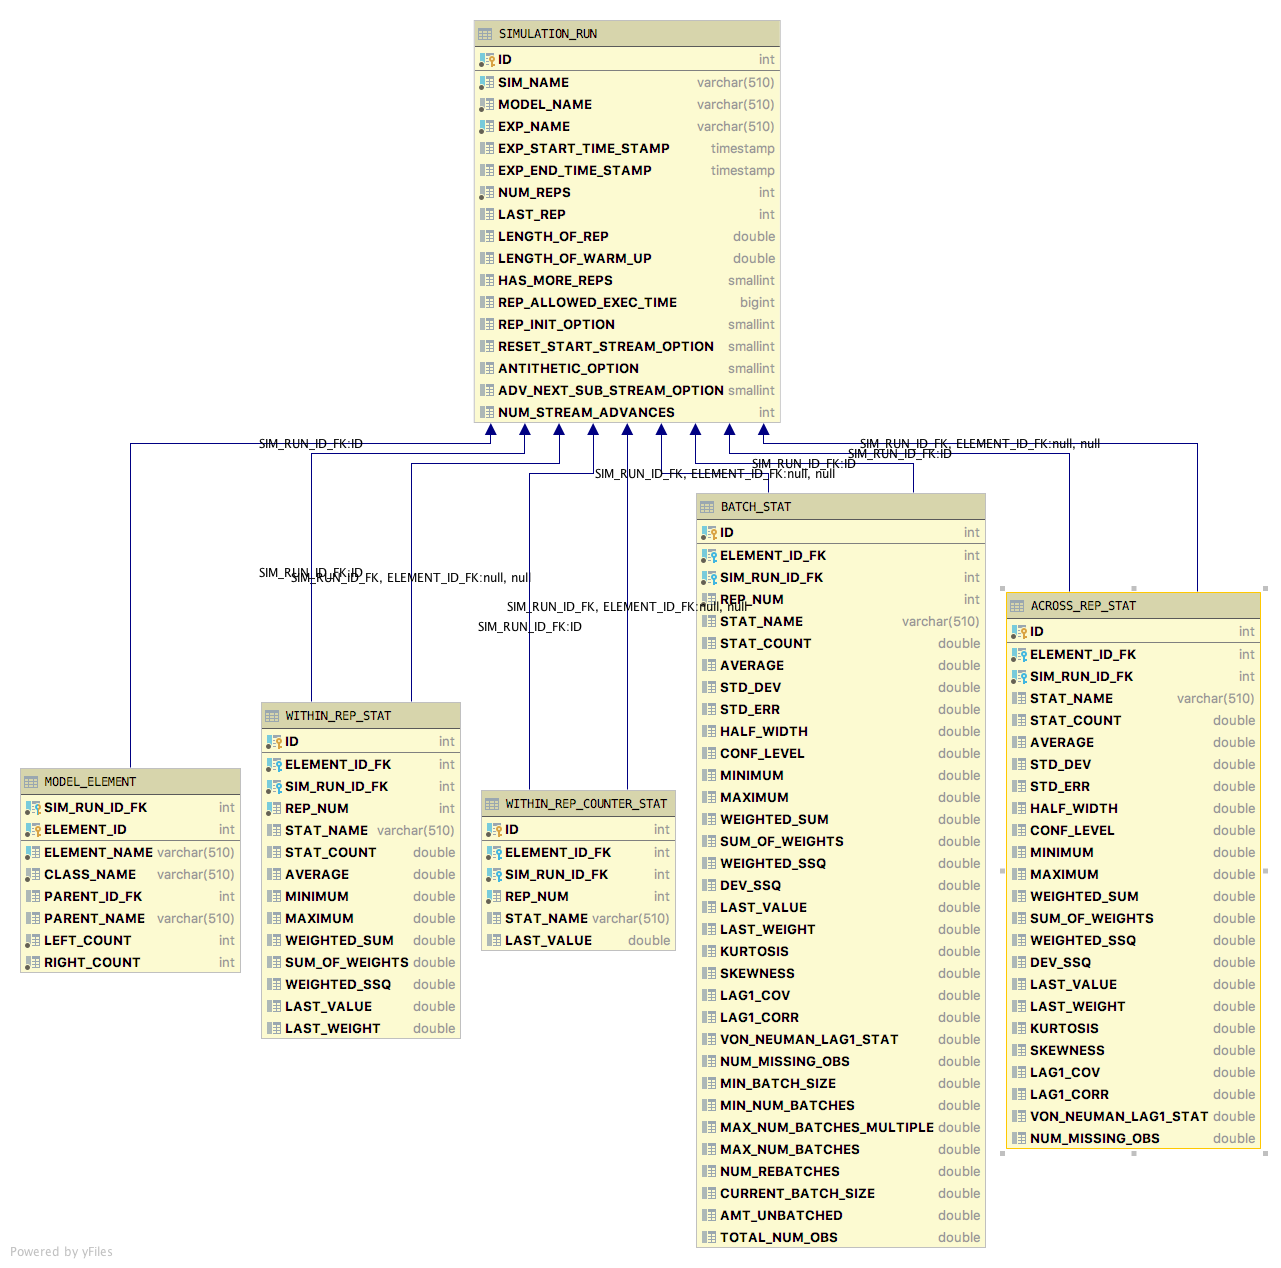
\includegraphics{./figures/JSLDBTables.png}
\caption{\label{fig:JSLDBTables}JSL Database Relational Diagram}
\end{figure}

\begin{figure}
\centering
\includegraphics{./figures/JSLDBViews.png}
\caption{\label{fig:JSLDBViews}JSL Database Views}
\end{figure}

The information within the SIMULATION\_RUN, MODEL\_ELEMENT,
WITHIN\_REP\_STAT, WITHIN\_REP\_COUNTER\_STAT tables are written to the
database at the end of each replication. The ACROSS\_REP\_STAT and
BATCH\_STAT tables are filled after the entire experiment is completed.
Even though the ACROSS\_REP\_STAT table could be constructed directly
from the data captured within the tables holding with replication data,
this is not done. Instead, the across replication statistics are
directly written from the simulation after all replications of an
experiment are completed.

A JSLDatabase instance is constructed to hold the data from any JSL
simulation. As such, a simulation execution can have many observers and
thus could have any number of JSLDatabase instances that collect data
from the execution. The most common case for multiple databases would be
the use of an embedded database as well as a database that is stored on
a database server.

\hypertarget{creating-and-using-a-default-jsl-database}{%
\subsection{Creating and Using a Default JSL Database}\label{creating-and-using-a-default-jsl-database}}

It is easy to have a database associated with a simulation. Just
indicate that a default database should be created when constructing an
instance of the Simulation class by providing ``true'' for the create
default database parameter of the Simulation class:

\begin{Shaded}
\begin{Highlighting}[]
\NormalTok{Simulation sim }\OperatorTok{=} \KeywordTok{new} \FunctionTok{Simulation}\OperatorTok{(}\StringTok{"Drive Through Pharmacy"}\OperatorTok{,} \KeywordTok{true}\OperatorTok{);}
\end{Highlighting}
\end{Shaded}

This causes an instance of the class, JSLDatabase, to be created and
attached to the instance of the Simulation as an observer via an
intermediate class called JSLDatabaseObserver. The running of the
simulation then causes data from the simulation to be stored in an
Apache Derby embedded database that is contained within the directory,
jslOutput/db. The name of the database will be based on the name
provided for the simulation. For the previous code snippet, a database
called JSLDb\_DriveThroughPharmacy will be created. Any spaces in the
name of the simulation are removed for the name of the database and
JSLDb\_ is appended. This naming is the default behavior for the default
database. The database can be accessed just like any database. For
example, IntelliJ's Datagrip tool can be used to connect to the
database, execute queries, and export data.

One very important point to note is that constructing an instance of
Simulation and providing ``true'' for the create default database option,
\textbf{always} creates a new instance of the default database. This process
involves deleting the previous default database and re-creating it
without any data. If you do not want the previously created default
database to be deleted and recreated, then you must take explicit steps
to prevent this from happening. The most obvious steps include:

\begin{itemize}
\tightlist
\item
  Do not call the constructor of Simulation with ``true'' for the create
  default database option. This will cause no new default JSL database
  to be created. Thus, a previous database instance will not be
  deleted. Or,
\item
  Change the name of the simulation so that a differently named
  default database will be constructed.
\item
  Move, copy, or rename the previously created database using
  operating system commands.
\end{itemize}

Note that if you execute \textbf{any} simulation that has the \textbf{same name}
as a previously executed simulation and you were using the default
database option, then the previous database will be deleted and
recreated. This might cause you to lose previous simulation results.
This behavior is the default because generally, when you re-run your
simulation you want the results of that run to be written into the
database.

\hypertarget{creating-and-using-jsl-databases}{%
\subsection{Creating and Using JSL Databases}\label{creating-and-using-jsl-databases}}

To better control the creation and use of an instance of the
JSLDatabase, I suggest that you consider creating your own instance
rather than relying on the default database. The main reason to do this
is if you plan to add results from multiple simulation executions to the
\textbf{same} database. A database represented by a JSLDatabase instance is
just a database that has a JSL\_DB schema within it to hold data from a
JSL simulation run. Provided that you can properly configure a JSL\_DB
schema within a database, you can use \textbf{any} database as the backing
store for JSL results. By default the JSL library facilitates the
creation of embedded Apache Derby databases and PostgreSQL databases. In
addition, the JSL library facilitates the creation of JSLDatabase
instances based on these two database management systems.

A number of methods are provided to create instances of a JSLDatabase.
Obviously, the constructor of JSLDatabase can be used. The constructor
has two parameters, an instance of an object that implements the
DatabaseIfc interface and a Boolean parameter (clearDataOption) which
controls whether or not all of the data within a possible JSL\_DB schema
is removed when the JSLDatabase instance is created. The default
behavior is to not remove previous data. If the supplied DatabaseIfc
interface instance does not already have a JSL\_DB schema, then one is
created. If it already has a JSL\_DB schema, then the clear data option
controls what happens to any previously stored data. Any of the methods
of the DatabaseFactory class can be used to create an instance of the
DatabaseIfc interface. Because you are most likely interested in
directly making a JSLDatabase instance, there are a number of static
methods of the JSLDatabase class that are provided for common use cases.
For example, the following code snippet illustrates how to make an
instance of a JSLDatabase based on the embedded Derby database system.
This will create a database named ``MCB\_Db'' within the jslOutput/db
directory. If a database already exists with that name, then it will be
deleted and a new database created.

\begin{Shaded}
\begin{Highlighting}[]
\NormalTok{JSLDatabase mcb\_db }\OperatorTok{=}\NormalTok{ JSLDatabase}\OperatorTok{.}\FunctionTok{createEmbeddedDerbyJSLDatabase}\OperatorTok{(}\StringTok{"MCB\_Db"}\OperatorTok{);}
\end{Highlighting}
\end{Shaded}

If you want to connect to a previously created database, then use the
methods of the DatabaseFactory class. For example, the following
connects to an existing database found within the jslOutput/db directory
and then supplies it to the JSLDatabase constructor. No previous data is
lost via this process since we are only connecting to a database (not
creating one).

\begin{Shaded}
\begin{Highlighting}[]
\NormalTok{DatabaseIfc database }\OperatorTok{=}\NormalTok{ DatabaseFactory}\OperatorTok{.}\FunctionTok{getEmbeddedDerbyDatabase}\OperatorTok{(}\StringTok{"JSLDb\_DriveThroughPharmacy"}\OperatorTok{);}
\CommentTok{// use the database as the backing database for the new JSLDatabase instance}
\NormalTok{JSLDatabase jslDatabase }\OperatorTok{=} \KeywordTok{new} \FunctionTok{JSLDatabase}\OperatorTok{(}\NormalTok{database}\OperatorTok{);}
\end{Highlighting}
\end{Shaded}

The previously illustrated code examples only \textbf{create} an instance of
JSLDatabase. The instance is \textbf{not} connected to an instance of
Simulation and thus simulation results will not be added to the database
unless additional steps are taken to hook up the JSLDatabase instance
with instances of the Simulation class prior to running experiments.

The approach to connect a JSLDatabase instance with a Simulation
instance involves creating an instance of JSLDatabaseObserver to monitor
the simulation's execution. JSLDatabaseObserver has three required
parameters in its constructor: 1) an instance of JSLDatabase, 2) and
instance of Simulation, and 3) a boolean parameter
(clearDataBeforeExperimentOption), which controls whether or not data
from prior executions of the observed simulation will be cleared if they
have the same simulation name and experiment name before each experiment
(i.e.~when the run() method is called on the simulation). The default
value for the clear data before experiment option is true. Thus, data
will be cleared from the database if the simulation name and experiment
name are \textbf{the same}. If you do not want the data cleared, then set the
option to false. However, if you then attempt to execute a simulation
that has the same name and experiment name as one already stored in the
database, an exception will be thrown. To prevent this exception change
the name of the simulation or the experiment prior to running the
simulation or decide to clear the data. The preferred method is to
change the name of the experiment since this facilitates other analysis
using JSL constructs.

Since creating and using a JSLDatabaseObserver is a common use case, the
JSL library provides methods on the Simulation class to facilitate this:

\begin{itemize}
\tightlist
\item
  \texttt{public\ JSLDatabaseObserver\ createJSLDatabaseObserver(String\ dbName)}
\item
  \texttt{public\ JSLDatabaseObserver\ createJSLDatabaseObserver(JSLDatabase\ jslDatabase)}
\item
  \texttt{public\ JSLDatabaseObserver\ createJSLDatabaseObserver(JSLDatabase\ jslDatabase,\ boolean\ clearDataBeforeExperiment)}
\end{itemize}

The first method creates an embedded Derby database with the provided
name in the jslOutput/db directory. The created JSLDatabaseObserver is
returned and through that reference the underlying JSLDatabase can be
accessed. The first of these three methods creates a new database. The
latter two only creates a new JSLDatabaseObserver instance and uses the
supplied JSLDatabase. Thus, data will be added to the database. The
class, UsingJSLDbExamples within the ex.running package illustrates many
of the use cases presented.

As an illustration consider running a simulation multiple times within
the same program execution but with different parameters. The following
code illustrates how this might be achieved. The first line creates a
simulation with a default database. Then the simulation is set up and
executed. Notice that the experiment name is set prior to running the
simulation. Then, the service time parameter is changed and the
simulation is executed again. Notice that the experiment name was
changed before the second simulation run. Data from both executions are
captured within the default database. This code can be re-executed
because a new default database is created each the Simulation instance
is constructed. This clears all previous data and then all subsequent
runs are captured because the experiment name is changed. If the name
had not been changed before the second simulation run, then when the
second simulation run executes the data from the first run will be
cleared and the second run data captured because the clear data before
experiment flag is true. If the clear data before experiment flag is
false and you attempt to execute this code an exception would be thrown
because there would be an attempt to enter data into the database that
has the same simulation and experiment name. This would force you to
change the name of the experiment before executing the second
experiment. Because this code does change the names of the experiments,
the clear data before experiment flag setting is irrelevant because the
experiments have different names.

\begin{Shaded}
\begin{Highlighting}[]
\CommentTok{// make the simulation with a default database}
\NormalTok{Simulation sim }\OperatorTok{=} \KeywordTok{new} \FunctionTok{Simulation}\OperatorTok{(}\StringTok{"MultiRun"}\OperatorTok{,} \KeywordTok{true}\OperatorTok{);}
\CommentTok{// set the parameters of the experiment}
\NormalTok{sim}\OperatorTok{.}\FunctionTok{setNumberOfReplications}\OperatorTok{(}\DecValTok{30}\OperatorTok{);}
\NormalTok{sim}\OperatorTok{.}\FunctionTok{setLengthOfReplication}\OperatorTok{(}\FloatTok{20000.0}\OperatorTok{);}
\NormalTok{sim}\OperatorTok{.}\FunctionTok{setLengthOfWarmUp}\OperatorTok{(}\FloatTok{5000.0}\OperatorTok{);}

\CommentTok{// create the model element and attach it to the main model}
\NormalTok{DriverLicenseBureauWithQ driverLicenseBureauWithQ }\OperatorTok{=} \KeywordTok{new} \FunctionTok{DriverLicenseBureauWithQ}\OperatorTok{(}\NormalTok{sim}\OperatorTok{.}\FunctionTok{getModel}\OperatorTok{());}
\NormalTok{sim}\OperatorTok{.}\FunctionTok{setExperimentName}\OperatorTok{(}\StringTok{"1stRun"}\OperatorTok{);}
\CommentTok{// tell the simulation to run}
\BuiltInTok{System}\OperatorTok{.}\FunctionTok{out}\OperatorTok{.}\FunctionTok{println}\OperatorTok{(}\StringTok{"Simulation started."}\OperatorTok{);}
\NormalTok{sim}\OperatorTok{.}\FunctionTok{run}\OperatorTok{();}
\BuiltInTok{System}\OperatorTok{.}\FunctionTok{out}\OperatorTok{.}\FunctionTok{println}\OperatorTok{(}\StringTok{"Simulation completed."}\OperatorTok{);}

\NormalTok{sim}\OperatorTok{.}\FunctionTok{setExperimentName}\OperatorTok{(}\StringTok{"2ndRun"}\OperatorTok{);}
\NormalTok{driverLicenseBureauWithQ}\OperatorTok{.}\FunctionTok{setServiceDistributionInitialRandomSource}\OperatorTok{(}\KeywordTok{new} \FunctionTok{ExponentialRV}\OperatorTok{(}\FloatTok{0.7}\OperatorTok{));}

\CommentTok{// tell the simulation to run}
\BuiltInTok{System}\OperatorTok{.}\FunctionTok{out}\OperatorTok{.}\FunctionTok{println}\OperatorTok{(}\StringTok{"Simulation started."}\OperatorTok{);}
\NormalTok{sim}\OperatorTok{.}\FunctionTok{run}\OperatorTok{();}
\BuiltInTok{System}\OperatorTok{.}\FunctionTok{out}\OperatorTok{.}\FunctionTok{println}\OperatorTok{(}\StringTok{"Simulation completed."}\OperatorTok{);}

\CommentTok{// get the default JSL database}
\NormalTok{Optional}\OperatorTok{\textless{}}\NormalTok{JSLDatabase}\OperatorTok{\textgreater{}}\NormalTok{ db }\OperatorTok{=}\NormalTok{ sim}\OperatorTok{.}\FunctionTok{getDefaultJSLDatabase}\OperatorTok{();}
\ControlFlowTok{if} \OperatorTok{(}\NormalTok{db}\OperatorTok{.}\FunctionTok{isPresent}\OperatorTok{())} \OperatorTok{\{}
    \BuiltInTok{System}\OperatorTok{.}\FunctionTok{out}\OperatorTok{.}\FunctionTok{println}\OperatorTok{(}\StringTok{"Printing across replication records"}\OperatorTok{);}
\NormalTok{    db}\OperatorTok{.}\FunctionTok{get}\OperatorTok{().}\FunctionTok{getAcrossRepStatRecords}\OperatorTok{().}\FunctionTok{format}\OperatorTok{(}\BuiltInTok{System}\OperatorTok{.}\FunctionTok{out}\OperatorTok{);}
    \BuiltInTok{System}\OperatorTok{.}\FunctionTok{out}\OperatorTok{.}\FunctionTok{println}\OperatorTok{();}
\OperatorTok{\}}
\end{Highlighting}
\end{Shaded}

Once you have a database that contains the schema to hold JSL based
data, you can continue to write results to that database as much as you
want. If your database is on a server, then you can easily collect data
from different simulation executions that occur on different computers
by referencing the database on the server. Therefore, if you are running
multiple simulation runs in parallel on different computers or in the
``cloud'', you should be able to capture the data from the simulation runs
into one database.

\hypertarget{querying-the-jsl-database}{%
\subsection{Querying the JSL Database}\label{querying-the-jsl-database}}

The JSL database is a database and thus it can be queried from within
Java or from other programs. If you have an instance of the JSLDatabase
as in:

\begin{Shaded}
\begin{Highlighting}[]
\NormalTok{DatabaseIfc database }\OperatorTok{=}\NormalTok{ DatabaseFactory}\OperatorTok{.}\FunctionTok{getEmbeddedDerbyDatabase}\OperatorTok{(}\StringTok{"JSLDb\_DriveThroughPharmacy"}\OperatorTok{);}
\CommentTok{// use the database as the backing database for the new JSLDatabase instance}
\NormalTok{JSLDatabase jslDatabase }\OperatorTok{=} \KeywordTok{new} \FunctionTok{JSLDatabase}\OperatorTok{(}\NormalTok{database}\OperatorTok{);}
\end{Highlighting}
\end{Shaded}

You can extract information about the simulation run using the methods
of the JSLDatabase class. Since the underlying data is stored in a
relational database, SQL queries can be used on the database. The
discussion of writing and executing queries from within Java is beyond
the scope of this discussion. To facilitate queries within Java, the JSL
leverages the open source jooQ library. A few methods to be aware of
include:

\begin{itemize}
\tightlist
\item
  \texttt{writeAllTablesAsCSV()} -- writes all the tables to separate CSV files
\item
  \texttt{writeDbToExcelWorkbook()} -- writes all the tables and views to a single Excel workbook
\item
  \texttt{getWithinRepViewRecords()} -- returns a jooQ Result containing all the within replication statistical records
\item
  \texttt{getWithinRepViewRecordsAsTablesawTable()} -- returns a Tablesaw table representation of the within replication statistical data
\item
  \texttt{getAcrossRepViewRecordsAsTablesawTable()} -- returns a Tablesaw table
  representation of the across replication statistical data
\item
  \texttt{getAcrossRepViewRecords()} -- returns a jooQ Result containing all the
  across replication statistical records
\item
  \texttt{getMultipleComparisonAnalyserFor(set\ of\ experiment\ name,\ response\ \ \ \ \ name)} -- returns an instance of the MultipleComparisonAnalyzer class
  in order to perform a multiple comparison analysis of a set of
  experiments on a specific response name.
\end{itemize}

The JSL database can be accessed via R or other software programs and
additional analysis performed on JSL simulation data.

\hypertarget{additional-functionality}{%
\subsection{Additional Functionality}\label{additional-functionality}}

The functionality of the JSL\_DB depends upon how ResponseVariable,
TimeWeighted, and Counter instances are named within a JSL model. A JSL
model is organized into a tree of ModelElement instances with the
instance of the Model at the top of the tree. The Model instance for the
simulation model contains instances of ModelElement, which are referred
to as children of the parent model element. Each model element instance
can have zero or more children, and those children can have children,
etc. Each ModelElement instance must have a unique integer ID and a
unique name. The unique integer ID is automatically provided when a
ModelElement instance is created. The user can supply a name for a
ModelElement instance when creating the instance. The name must be
unique within the simulation model.

A recommended practice to ensure that model element names are unique is
to use the name of the parent model element as part of the name. If the
parent name is unique, then all children names will be unique relative
to any other model elements. For example, in the following code
getName() references the name of the current model element (an instance
of QueueingSystemWithQ), which is serving as the parent for the children
model element declared within the constructor.

\begin{Shaded}
\begin{Highlighting}[]
\KeywordTok{public} \FunctionTok{QueueingSystemWithQ}\OperatorTok{(}\NormalTok{ModelElement parent}\OperatorTok{,} \DataTypeTok{int}\NormalTok{ numServers}\OperatorTok{,}\NormalTok{ RVariableIfc ad}\OperatorTok{,}\NormalTok{ RVariableIfc sd}\OperatorTok{)} \OperatorTok{\{}
    \KeywordTok{super}\OperatorTok{(}\NormalTok{parent}\OperatorTok{);}

\NormalTok{    myWaitingQ }\OperatorTok{=} \KeywordTok{new} \BuiltInTok{Queue}\OperatorTok{(}\KeywordTok{this}\OperatorTok{,} \FunctionTok{getName}\OperatorTok{()} \OperatorTok{+} \StringTok{"\_Q"}\OperatorTok{);}
\NormalTok{    myNumBusy }\OperatorTok{=} \KeywordTok{new} \FunctionTok{TimeWeighted}\OperatorTok{(}\KeywordTok{this}\OperatorTok{,} \FloatTok{0.0}\OperatorTok{,} \FunctionTok{getName}\OperatorTok{()} \OperatorTok{+} \StringTok{"\_NumBusy"}\OperatorTok{);}
\NormalTok{    myNS }\OperatorTok{=} \KeywordTok{new} \FunctionTok{TimeWeighted}\OperatorTok{(}\KeywordTok{this}\OperatorTok{,} \FloatTok{0.0}\OperatorTok{,} \FunctionTok{getName}\OperatorTok{()} \OperatorTok{+} \StringTok{"\_NS"}\OperatorTok{);}
\NormalTok{    mySysTime }\OperatorTok{=} \KeywordTok{new} \FunctionTok{ResponseVariable}\OperatorTok{(}\KeywordTok{this}\OperatorTok{,} \FunctionTok{getName}\OperatorTok{()} \OperatorTok{+} \StringTok{"\_System Time"}\OperatorTok{);}
\end{Highlighting}
\end{Shaded}

The name supplied to the TimeWeighted and ResponseVariable constructors
will cause the underlying statistic to have the same name. The
statistic's name cannot be changed once it is set. The statistic name is
important for referencing statistical data within the JSL database. One
complicating factor involves using the JSL database to analyze the
results from multiple simulation models. In order to more readily
compare the results of the same performance measure between two
different simulation models, the user should try to ensure that the
names of the performance measures are the same. If the above recommended
naming practice is used, the names of the statistics may depend on the
order in which the model element instances are created and added to the
model element hierarchy. If the model structure never changes between
different simulation models then this will not present an issue;
however, if the structure of the model changes between two different
simulation models (which can often be the case), the statistic names may
be affected. If this issue causes problems, you can always name the
desired output responses or counters exactly what you want it to be and
use the same name in other simulation models.

Since the model element ID is assigned automatically based on the number
of model elements created within the model, the model element numbers
between two instances of the same simulation model will most likely be
different. Thus, there is no guarantee that the IDs will be the same and
using the model element ID as part of queries on the JSL database will
have to take this into account. You can assume that the name of the
underlying statistic is the same as its associated model element and
since it is user definable, it is better suited for queries based on the
JSL database.

\clearpage

\hypertarget{app:rnrv}{%
\chapter{Generating Pseudo-Random Numbers and Random Variates}\label{app:rnrv}}

\textbf{\textsc{Learning Objectives}}

\begin{itemize}
\item
  To be able to describe and use linear congruential pseudo-random
  number generation methods
\item
  To be aware of current state of the art pseudo-random number
  generation methods
\item
  To be able to define and use key terms in pseudo-random number
  generation methods such as streams, seeds, period, etc.
\item
  To be able to explain the key issues in pseudo-random number testing
\item
  To be able to derive and implement an inverse cumulative
  distribution function based random variate generation algorithm
\item
  To be able to explain and implement the convolution algorithm for
  random variate generation
\item
  To be able to explain and implement the acceptance rejection
  algorithm for random variate generation
\end{itemize}

Randomness in simulation is often modeled by using
random variables and probability distributions. Thus, simulation
languages require the ability to generate random variates. A random
variate is an instance (or realization) of a random variable. In this
section, you will learn how simulation languages allow for the
generation of randomness. Generating randomness requires algorithms that
permit sequences of numbers to act as the underlying source of
randomness within the model. Then, given a good
source of randomness, techniques have been established that permit the
sequences to be transformed so that they can represent a wide variety of
random variables (e.g.~normal, Poisson, etc.). The algorithms that
govern these procedures are described in the second part of this chapter.

\hypertarget{app:rnrv:rn}{%
\section{Pseudo Random Numbers}\label{app:rnrv:rn}}

This section indicates how uniformly distributed random numbers over
the range from 0 to 1 are obtained within simulation programs. While
commercial simulation packages provide substantial capabilities for
generating random numbers, we still need to understand how this process
works for the following reasons:

\begin{enumerate}
\def\labelenumi{\arabic{enumi}.}
\item
  The random numbers within a simulation experiment might need to be
  controlled in order to take advantage of them to improve decision
  making.
\item
  In some situations, the commercial package does not have ready made
  functions for generating the desired random variables. In these
  situations, you will have to implement an algorithm to generate the random variates.
\end{enumerate}

In addition, simulation is much broader than just using a commercial
package. You can perform simulation in any computer language and spreadsheets. The
informed modeler should know how the key inputs to simulation models are
generated.

In simulation, large amount of cheap (easily computed) random numbers
are required. In general, consider how random numbers might be obtained:

\begin{enumerate}
\def\labelenumi{\arabic{enumi}.}
\item
  Dice, coins, colored balls
\item
  Specially designed electronic equipment
\item
  Algorithms
\end{enumerate}

Clearly, within the context of computer simulation, it might be best to
rely on algorithms; however, if an algorithm is used to generate the
random numbers then they will not be truly random. For this reason, the
random numbers that are used in computer simulation are called \emph{pseudo
random}.

\begin{center}\rule{0.5\linewidth}{0.5pt}\end{center}

\begin{definition}[Pseudo-Random Numbers]
\protect\hypertarget{def:PRN}{}{\label{def:PRN} \iffalse (Pseudo-Random Numbers) \fi{} }A sequence of pseudo-random numbers, \(U_{i}\), is a deterministic sequence of numbers in \((0,1)\) having the same relevant statistical properties as a sequence of truly
random \(U(0,1)\) numbers.(\citep{ripley1987stochastic})
\end{definition}

\begin{center}\rule{0.5\linewidth}{0.5pt}\end{center}

A set of statistical tests are performed on the pseudo-random numbers
generated from algorithms in order to indicate that their properties are
not significantly different from a true set of \(U(0,1)\) random numbers.
The \emph{algorithms} that produce pseudo-random numbers are called \emph{random number generators}. In addition to passing a battery of statistical tests, the random
number generators need to be fast and they need to be able to reproduce
a sequence of numbers if and when necessary.

The following section discusses random number generation methods. The
approach will be practical, with just enough theory to motivate future
study of this area and to allow you to understand the important
implications of random number generation. A more rigorous treatment of
random number and random variable generation can be found such texts as
\citep{fishman2006first} and \citep{devroye1986nonuniform}.

\hypertarget{app:rnrv:rngs}{%
\subsection{Random Number Generators}\label{app:rnrv:rngs}}

Over the history of scientific computing, there have been a wide variety
of techniques and algorithms proposed and used for generating
pseudo-random numbers. A common technique that has been used (and is
still in use) within a number of simulation environments is discussed in
this text. Some new types of generators that have been recently adopted
within many simulation environments, especially the one used within the
\href{https://rossetti.git-pages.uark.edu/jslbookdownbook/}{JSL} and Arena, will also be briefly discussed.

A linear congruential generator (LCG) is a recursive algorithm for
producing a sequence of pseudo random numbers. Each new pseudo random
number from the algorithm depends on the previous pseudo random number.
Thus, a starting value called the \emph{seed} is required. Given the value of
the seed, the rest of the sequence of pseudo random numbers can be
completely determined by the algorithm. The basic definition of an LCG
is as follows

\begin{center}\rule{0.5\linewidth}{0.5pt}\end{center}

\begin{definition}[Linear Congruential Generator]
\protect\hypertarget{def:LCG}{}{\label{def:LCG} \iffalse (Linear Congruential Generator) \fi{} }A LCG defines a sequence of
integers, \(R_{0}, R_{1}, \ldots\) between \(0\) and \(m-1\) according to the
following recursive relationship:

\[
R_{i+1} = \left(a R_{i} + c\right)\bmod m %) %\left(m\right)
\]

where \(R_{0}\) is called the seed of the sequence, \(a\) is called the
constant multiplier, \(c\) is called the increment, and \(m\) is called the
modulus. \(\left(m, a, c, R_{0}\right)\) are integers with \(a > 0\),
\(c \geq 0\), \(m > a\), \(m > c\), \(m > R_{0}\), and \(0 \leq R_{i} \leq m-1\).

To compute a corresponding pseudo-random uniform number, we use

\[
U_{i} = \frac{R_{i}}{m}
\]
\end{definition}

\begin{center}\rule{0.5\linewidth}{0.5pt}\end{center}

Notice that an LCG defines a sequence of integers and subsequently a
sequence of real (rational) numbers that can be considered pseudo random
numbers. Remember that pseudo random numbers are those that can ``fool'' a
battery of statistical tests. The choice of the seed, constant
multiplier, increment, and modulus, i.e.~the parameters of the LCG, will
determine the properties of the sequences produced by the generator.
With properly chosen parameters, an LCG can be made to produce pseudo
random numbers. To make this concrete, let's look at a simple example of
an LCG.

\begin{center}\rule{0.5\linewidth}{0.5pt}\end{center}

\begin{example}[Simple LCG Example]
\protect\hypertarget{exm:SimpleLCG}{}{\label{exm:SimpleLCG} \iffalse (Simple LCG Example) \fi{} }Consider an LCG
with the following parameters \((m = 8\), \(a = 5\), \(c = 1\), \(R_{0} = 5)\). Compute
the first nine values for \(R_{i}\) and \(U_{i}\) from the defined
sequence.
\end{example}
***

Let's first remember how to compute using the \(\bmod\) operator. The
\(\bmod\) operator is defined as:

\[
z = y \bmod m = y - m \left \lfloor \dfrac{y}{m} \right \rfloor
\]

where \(\lfloor x \rfloor\) is the floor operator, which returns the
greatest integer that is less than or equal to \(x\). For example,

\begin{equation}
\begin{split}
z & = 17 \bmod 3 \\
  & = 17 - 3 \left \lfloor \frac{17}{3} \right \rfloor \\
  & = 17 - 3 \lfloor 5.\overline{66} \rfloor \\
  & = 17 - 3 \times 5 = 2
\end{split}
\end{equation}

Thus, the \(\bmod\) operator returns the integer remainder (including zero) when \(y \geq m\) and \(y\) when \(y < m\). For example,
\(z = 6 \bmod 9 = 6 - 9 \left\lfloor \frac{6}{9} \right\rfloor = 6 - 9 \times 0 = 6\).

Using the parameters of the LCG, the pseudo-random numbers are:

\[
\begin{split}
  {R_1} & = (5{R_0} + 1)\bmod 8 = 26\bmod 8 = 2 \Rightarrow {U_1} = 0.25  \\
  {R_2} & =  (5{R_1} + 1)\bmod 8 = 11\bmod 8 = 3 \Rightarrow {U_2} = 0.375  \\
  {R_3} & =  (5{R_2} + 1)\bmod 8 = 16\bmod 8 = 0 \Rightarrow {U_3} = 0.0  \\
  {R_4} & =  (5{R_3} + 1)\bmod 8 = 1\bmod 8 = 1 \Rightarrow {U_4} = 0.125  \\
  {R_5} & =  6 \Rightarrow {U_5} = 0.75 \\
  {R_6} & =  7 \Rightarrow {U_6} = 0.875 \\
  {R_7} & =  4 \Rightarrow {U_7} = 0.5 \\
  {R_8} & =  5 \Rightarrow {U_8} = 0.625 \\
  {R_9} & =  2 \Rightarrow {U_9} = 0.25
\end{split}
\]

In the previous example, the \(U_{i}\) are simple fractions involving
\(m = 8\). Certainly, this sequence does not appear very random. The
\(U_{i}\) can only take on rational values in the range,
\(0,\tfrac{1}{m}, \tfrac{2}{m}, \tfrac{3}{m}, \ldots, \tfrac{(m-1)}{m}\)
since \(0 \leq R_{i} \leq m-1\). This implies that if \(m\) is small there
will be gaps on the interval \(\left[0,1\right)\), and if \(m\) is large
then the \(U_{i}\) will be more densely distributed on \(\left[0,1\right)\).

Notice that if a sequence generates the same value as a previously
generated value then the sequence will repeat or cycle. An important
property of a LCG is that it has a long cycle, as close to length \(m\) as
possible. The length of the cycle is called the \emph{period} of the LCG.
Ideally the period of the LCG is equal to \(m\). If this occurs, the LCG
is said to achieve its full period. As can be seen in the example, the
LCG is full period. Until recently, most computers were 32 bit machines
and thus a common value for \(m\) is \(2^{31} - 1 = 2,147,483,647\), which
represents the largest integer number on a 32 bit computer using 2's
complement integer arithmetic. This choice of \(m\) also happens to be a
prime number, which leads to special properties.

A proper choice of the parameters of the LCG will allow desirable pseudo
random number properties to be obtained. The following result due to
\citep{hull1962random}, see also \citep{law2007simulation}, indicates how to check
if a LCG will have the largest possible cycle.

\begin{center}\rule{0.5\linewidth}{0.5pt}\end{center}

\begin{theorem}[LCG Theorem]
\protect\hypertarget{thm:LCGThm}{}{\label{thm:LCGThm} \iffalse (LCG Theorem) \fi{} }An LCG has full period if and only if the following three conditions hold: (1) The only positive integer that (exactly) divides both \(m\) and \(c\) is 1 (i.e.~\(c\) and \(m\) have no common factors other than 1), (2) If \(q\) is a prime number that divides \(m\) then \(q\) should divide \((a-1)\). (i.e.~\((a-1)\) is a multiple of every prime number that divides \(m\)), and (3) If 4 divides \(m\), then 4 should divide \((a-1)\). (i.e.~\((a-1)\) is a multiple of 4 if \(m\) is a multiple of 4)
\end{theorem}

\begin{center}\rule{0.5\linewidth}{0.5pt}\end{center}

Now, let's apply this theorem to the example LCG and check whether or
not it should obtain full period. To apply the theorem, you must check if each of the three conditions
holds for the generator.

\begin{itemize}
\item
  Condition 1: \(c\) and \(m\) have no common factors other than 1.\\
  The factors of \(m=8\) are \((1, 2, 4, 8)\), since \(c=1\) (with factor 1)
  condition 1 is true.
\item
  Condition 2: \((a-1)\) is a multiple of every prime number that
  divides \(m\). The first few prime numbers are (1, 2, 3, 5, 7). The
  prime numbers, \(q\), that divide \(m=8\) are \((q =1, 2)\). Since \(a=5\)
  and \((a-1)=4\), clearly \(q = 1\) divides \(4\) and \(q = 2\) divides \(4\).
  Thus, condition 2 is true.
\item
  Condition 3: If \(4\) divides \(m\), then \(4\) should divide \((a-1)\).\\
  Since \(m=8\), clearly \(4\) divides \(m\). Also, \(4\) divides \((a-1)= 4\).
  Thus, condition 3 holds.
\end{itemize}

Since all three conditions hold, the LCG achieves full period.

\begin{rmdnote}
The theorem only tells us when a specification of \((a, c, m)\) will obtain full period. In case (3), it does not tell us anything about what happens if \(4\) does not divide \(m\), If \(4\) divides \(m\), and we pick \(a\) so that it divides \((a-1)\) then the condition will be met. If \(4\) does not divide \(m\), then the theorem really does not tell us one way or the other whether the LCG obtains full period.
\end{rmdnote}

There are some simplifying conditions, see \citet{banks2005discreteevent},
which allow for easier application of the theorem. For \(m = 2^{b}\), (\(m\)
a power of 2) and \(c\) not equal to 0, the longest possible period is \(m\)
and can be achieved provided that \(c\) is chosen so that the greatest
common factor of \(c\) and \(m\) is 1 and \(a=4k+1\) where \(k\) is an integer.
The previous example LCG satisfies this situation.

For \(m = 2^{b}\) and \(c = 0\), the longest possible period is \((m/4)\) and
can be achieved provided that the initial seed, \(R_{0}\) is odd and
\(a=8k + 3\) or \(a=8k + 5\) where \(k = 0, 1, 2,\cdots\).

The case of \(m\) a prime number and \(c = 0\), defines a special case of
the LCG called a \emph{prime modulus multiplicative linear congruential
generator} (PMMLCG). For this case, the longest possible period is \(m-1\)
and can be achieved if the smallest integer, \(k\), such that \(a^{k} -1\)
is divisible by \(m\) is \(m-1\).

Thirty-Two bit computers have been very common for over 20 years. In
addition, \(2^{31} - 1\) = \(2,147,483,647\) is a prime number. Because of
this, \(2^{31} - 1\) has been the choice for \(m\) with \(c=0\). Two common
values for the multiplier, \(a\), have been:

\[
\begin{split}
a & = 630,360,016\\
a & = 16,807\\
\end{split}
\]

The latter of which was used within many simulation packages for a number of years. Notice that for PMMLCG's the full period cannot be achieved (because \(c=0\)), but
with the proper selection of the multiplier, the next best period length
of \(m-1\) can be obtained. In addition, for this case
\(R_{0} \in \lbrace 1, 2,\ldots , m-1\rbrace\) and thus \(U_{i} \in (0,1)\).
The limitation of \(U_{i} \in (0,1)\) is very useful when generating
random variables from various probability distributions, since \(0\)
cannot be realized. When using an LCG, you must supply a starting seed
as an initial value for the algorithm. This seed determines the sequence
that will come out of the generator when it is called within software.
Since generators cycle, you can think of the sequence as a big circular
list as indicated in Figure \ref{fig:LCGCycle}.

\begin{figure}

{\centering \includegraphics[width=0.5\linewidth]{./figures2/AppRNRV/LCGCycle} 

}

\caption{Sequence for Simple LCG Example}\label{fig:LCGCycle}
\end{figure}

Starting with seed \(R_{0} = 5\), you get a sequence
\(\{2, 3, 0, 1, 6, 7, 4, 5\}\). Starting with seed, \(R_{0}=1\), you get the
sequence \(\{6, 7, 4, 5, 2, 3, 0, 1\}\). Notice that these two sequences
overlap with each other, but that the first half \(\{2, 3, 0, 1\}\) and
the second half \(\{6, 7, 4, 5\}\) of the sequence do not overlap. If you
only use 4 random numbers from each of these two \emph{subsequences} then the
numbers will not overlap. This leads to the definition of a stream:

\begin{center}\rule{0.5\linewidth}{0.5pt}\end{center}

\begin{definition}[Stream]
\protect\hypertarget{def:unnamed-chunk-1}{}{\label{def:unnamed-chunk-1} \iffalse (Stream) \fi{} }The subsequence of random numbers generated from a given seed is called a
random number stream.
\end{definition}

\begin{center}\rule{0.5\linewidth}{0.5pt}\end{center}

You can take the sequence produced by the random number generator and
divide it up into subsequences by associating certain seeds with
streams. You can call the first subsequence stream 1 and the second
subsequence stream 2, and so forth. Each stream can be further divided
into subsequences or sub-streams of non-overlapping random numbers.

In this simple example, it is easy to remember that stream 1 is defined
by seed, \(R_{0} = 5\), but when \(m\) is large, the seeds will be large
integer numbers, e.g.~\(R_{0} = 123098345\). It is difficult to remember
such large numbers. Rather than remember this huge integer, an
assignment of stream numbers to seeds is made. Then, the sequence can be
reference by its stream number. Naturally, if you are going to associate
seeds with streams you would want to divide the entire sequence so that
the number of non-overlapping random numbers in each stream is quite
large. This ensures that as a particular stream is used that there is
very little chance of continuing into the next stream. Clearly, you want
\(m\) to be as large as possible and to have many streams that contain as
large as possible number of non-overlapping random numbers. With today's
modern computers even \(m\) is \(2^{31} - 1 = 2,147,483,647\) is not very
big. For large simulations, you can easily run through all these random
numbers.

Random number generators in computer simulation languages come with a
default set of streams that divide the ``circle'' up into independent sets
of random numbers. The streams are only independent if you do not use up
all the random numbers within the subsequence. These streams allow the
randomness associated with a simulation to be controlled. During the
simulation, you can associate a specific stream with specific random
processes in the model. This has the advantage of allowing you to check
if the random numbers are causing significant differences in the
outputs. In addition, this allows the random numbers used across
alternative simulations to be better synchronized.

Now a common question for beginners using random number generators can
be answered. That is, \emph{If the simulation is using random numbers, why to
I get the same results each time I run my program?} The corollary to
this question is, \emph{If I want to get different random results each time I
run my program, how do I do it?} The answer to the first question is
that the underlying random number generator is starting with the same
seed each time you run your program. Thus, your program will use the
same pseudo random numbers today as it did yesterday and the day before,
etc. The answer to the corollary question is that you must tell the
random number generator to use a different seed (or alternatively a
different stream) if you want different invocations of the program to
produce different results. The latter is not necessarily a desirable
goal. For example, when developing your simulation programs, it is
desirable to have repeatable results so that you can know that your
program is working correctly. Unfortunately, many novices have heard
about using the computer clock to ``randomly'' set the seed for a
simulation program. This is a \emph{bad} idea and very much not recommended
in our context. This idea is more appropriate within a gaming
simulation, in order to allow the human gamer to experience different
random sequences.

Given current computing power, the previously discussed PMMLCGs are
insufficient since it is likely that all the 2 billion or so of the
random numbers would be used in performing serious simulation studies.
Thus, a new generation of random number generators was developed that
have extremely long periods. The random number generator described in
\citet{ecuyer2002an} is one example of such a generator. It is based on the
combination of two multiple recursive generators resulting in a period
of approximately \(3.1 \times 10^{57}\). This is the same generator that
is now used in many commercial simulation packages. The generator as
defined in \citep{law2007simulation} is:

\[
\begin{split}
R_{1,i}&=(1,403,580 R_{1,i-2} - 810,728 R_{1,i-3})[\bmod (2^{32}-209)]\\
R_{2,i}&=(527,612R_{2,i-1} - 1,370,589 R_{2,i-3})[\bmod (2^{32}-22,853)]\\
Y_i &=(R_{1,i}-R_{2,i})[\bmod(2^{32}-209)]\\
U_i&=\frac{Y_i}{2^{32}-209}
\end{split}
\]
The generator takes as its initial seed a vector of six initial values
\((R_{1,0}, R_{1,1}, R_{1,2}, R_{2,0}, R_{2,1}, R_{2,2})\). The first
initially generated value, \(U_{i}\), will start at index \(3\). To produce five pseudo random numbers using this generator we need an initial seed vector, such as:
\[\lbrace R_{1,0}, R_{1,1}, R_{1,2}, R_{2,0}, R_{2,1}, R_{2,2} \rbrace = \lbrace 12345, 12345, 12345, 12345, 12345, 12345\rbrace\]

Using the recursive equations, the resulting random numbers are as follows:

\begin{longtable}[]{@{}lcccccll@{}}
\toprule
& i=3 & i=4 & i=5 & i=6 & i=7 & & \\
\midrule
\endhead
\(Z_{1,i-3}=\) & 12345 & 12345 & 12345 & 3023790853 & 3023790853 & & \\
\(Z_{1,i-2}=\) & 12345 & 12345 & 3023790853 & 3023790853 & 3385359573 & & \\
\(Z_{1,i-1}=\) & 12345 & 3023790853 & 3023790853 & 3385359573 & 1322208174 & & \\
\(Z_{2,i-3}=\) & 12345 & 12345 & 12345 & 2478282264 & 1655725443 & & \\
\(Z_{2,i-2}=\) & 12345 & 12345 & 2478282264 & 1655725443 & 2057415812 & & \\
\(Z_{2,i-1}=\) & 12345 & 2478282264 & 1655725443 & 2057415812 & 2070190165 & & \\
\(Z_{1,i}=\) & 3023790853 & 3023790853 & 3385359573 & 1322208174 & 2930192941 & & \\
\(Z_{2,i}=\) & 2478282264 & 1655725443 & 2057415812 & 2070190165 & 1978299747 & & \\
\(Y_i=\) & 545508589 & 1368065410 & 1327943761 & 3546985096 & 951893194 & & \\
\(U_i=\) & 0.127011122076 & 0.318527565471 & 0.309186015655 & 0.82584686312 & 0.221629915834 & & \\
\bottomrule
\end{longtable}

While it is beyond the scope of this text to explore the theoretical
underpinnings of this generator, it is important to note that the use of
this new generator is conceptually similar to that which has already
been described. The generator allows multiple independent streams to be
defined along with sub-streams.

\begin{rmdnote}
A random number stream is a sub-sequence of pseudo-random numbers that start at particular place with a larger sequence of pseudo-random numbers. The starting point of a sequence of pseudo-random numbers is called the \emph{seed}. A seed allows us to pick a particular stream. Having multiple streams is useful to assign different streams to different sources of randomness within a model. Streams can be further divided into sub-streams. This facilitates the control of the use of pseudo-random numbers when performing experiments.
\end{rmdnote}

The fantastic thing about this generator is the sheer size of the
period. Based on their analysis, \citet{ecuyer2002an} state that it will be
``approximately 219 years into the future before average desktop
computers will have the capability to exhaust the cycle of the
(generator) in a year of continuous computing.'' In addition to the
period length, the generator has an enormous number of streams,
approximately \(1.8 \times 10^{19}\) with stream lengths of
\(1.7 \times 10^{38}\) and sub-streams of length \(7.6 \times 10^{22}\)
numbering at \(2.3 \times 10^{15}\) per stream. Clearly, with these
properties, you do not have to worry about overlapping random numbers
when performing simulation experiments. The generator was subjected to a
rigorous battery of statistical tests and is known to have excellent
statistical properties. The subject of modeling and testing different distributions is deferred to a separate part of this book.

\hypertarget{app:rnrv:rvs}{%
\section{Generating Random Variates from Distributions}\label{app:rnrv:rvs}}

In simulation, pseudo random numbers serve as the foundation for
generating samples from probability distribution models. We will now
assume that the random number generator has been rigorously tested and
that it produces sequences of \(U_{i} \sim U(0,1)\) numbers. We now want
to take the \(U_{i} \sim U(0,1)\) and utilize them to generate from
probability distributions.

The realized value from a probability distribution is called a random
variate. Simulations use many different probability distributions as
inputs. Thus, methods for generating random variates from distributions
are required. Different distributions may require different algorithms due to the challenges of efficiently producing the random variables. Therefore, we need to know how to generate samples from probability distributions. In generating random variates the goal is to produce samples \(X_{i}\) from a distribution \(F(x)\) given a source of random
numbers, \(U_{i} \sim U(0,1)\). There are four basic strategies or methods
for producing random variates:

\begin{enumerate}
\def\labelenumi{\arabic{enumi}.}
\tightlist
\item
  Inverse transform or inverse cumulative distribution function (CDF) method
\item
  Convolution
\item
  Acceptance/Rejection
\item
  Mixture and Truncated Distributions
\end{enumerate}

The following sections discuss each of these methods.

\hypertarget{inverse-transform-method}{%
\subsection{Inverse Transform Method}\label{inverse-transform-method}}

The inverse transform method is the preferred method for generating
random variates provided that the inverse transform of the cumulative
distribution function can be easily derived or computed numerically. The
key advantage for the inverse transform method is that for every \(U_{i}\)
use a corresponding \(X_{i}\) will be generated. That is, there is a one-to-one mapping between the pseudo-random number \(u_i\) and the generated variate \(x_i\).

The inverse transform technique utilizes the inverse of the cumulative
distribution function as illustrated in Figure \ref{fig:InvTrans}, will illustrates simple cumulative distribution function. First, generate a number, \(u_{i}\) between 0
and 1 (along the \(U\) axis), then find the corresponding \(x_{i}\)
coordinate by using \(F^{-1}(\cdot)\). For various values of \(u_{i}\), the
\(x_{i}\) will be properly `distributed' along the x-axis. The beauty of
this method is that there is a one to one mapping between \(u_{i}\) and
\(x_{i}\). In other words, for each \(u_{i}\) there is a unique \(x_{i}\)
because of the monotone property of the CDF.

\begin{figure}

{\centering \includegraphics[width=0.5\linewidth]{./figures2/AppRNRV/invTransFig} 

}

\caption{Inverse Transform Method}\label{fig:InvTrans}
\end{figure}

The idea illustrated in Figure \ref{fig:InvTrans} is based on the following theorem.

\begin{center}\rule{0.5\linewidth}{0.5pt}\end{center}

\begin{theorem}[Inverse Transform]
\protect\hypertarget{thm:InvTransThm}{}{\label{thm:InvTransThm} \iffalse (Inverse Transform) \fi{} }Let \(X\) be a random variable with \(X \sim F(x)\). Define another random variable \(Y\)
such that \(Y = F(X)\). That is, Y is determined by evaluating the
function \(F(\cdot)\) at the value \(X\). If \(Y\) is defined in this manner,
then \(Y \sim U(0,1)\).
\end{theorem}

\begin{center}\rule{0.5\linewidth}{0.5pt}\end{center}

The proof utilizes the definition of the cumulative distribution
function to derive the CDF for \(Y\).

\[
\begin{split}
F(y) & = P\left\{Y \leq y \right\}  \\
    & = P\left\{F(X) \leq y\right\}  \; \text{substitute for } Y \\
    & = P\left\{F^{-1}(F(X)) \leq F^{-1}(y)\right\}  \; \text{apply inverse} \\ 
    & = P\left\{X \leq F^{-1}(y)\right\}  \; \text{definition of inverse} \\ 
    & = F(F^{-1}(y)) \; \text{definition of CDF}\\ 
    & = y \; \text{definition of inverse} 
\end{split}
\]
Since \(P(Y \leq y) = y\) defines a \(U(0,1)\) random variable, the proof is
complete.

This result also works in reverse if you start with a uniformly
distributed random variable then you can get a random variable with the
distribution of \(F(x)\). The idea is to generate \(U_{i} \sim U(0,1)\) and
then to use the inverse cumulative distribution function to transform
the random number to the appropriately distributed random variate.

Let's assume that we have a function, \emph{randU01()}, that will provide
pseudo-random numbers on the range (0,1). Then, the following presents the pseudo-code for the inverse transform algorithm.

1. \(u = rand01()\)\\
2. \(x = F^{-1}(u)\)\\
3. return \(x\)

~

Line 1 generates a uniform number. Line 2 takes the inverse of \(u\) and line 3 returns the random variate. The following example illustrates the inverse transform method for the
exponential distribution.

The exponential distribution is often used to model the time until and event (e.g.~time
until failure, time until an arrival etc.) and has the following probability density function:

\[
f(x) =
\begin{cases}
0.0 & \text{if} \left\{x < 0\right\}\\
\lambda e^{-\lambda x} & \text{if} \left\{x \geq 0 \right\} \\
\end{cases}
\]
with
\[
\begin{split}
E\left[X\right] &= \frac{1}{\lambda} \\
Var\left[X\right] &= \frac{1}{\lambda^2}
\end{split}
\]

\begin{center}\rule{0.5\linewidth}{0.5pt}\end{center}

\begin{example}[Generating Exponential Random Variates]
\protect\hypertarget{exm:ExpInvCDF}{}{\label{exm:ExpInvCDF} \iffalse (Generating Exponential Random Variates) \fi{} }Consider a random variable, \(X\), that represents the time until failure for a machine tool. Suppose \(X\) is exponentially distributed with an expected value of \(1.\overline{33}\). Generate a random variate for the time until the first failure using a uniformly distributed value of \(u = 0.7\).
\end{example}

\begin{center}\rule{0.5\linewidth}{0.5pt}\end{center}

\textbf{Solution for Example \ref{exm:ExpInvCDF}} In order to solve this problem, we must first compute the CDF for the exponential distribution. For any value, \(b < 0\), we have by definition:

\[
F(b) = P\left\{X \le b \right\} = \int_{ - \infty }^b f(x)\;dx = \int\limits_{ - \infty }^b {0 dx} = 0
\]
For any value \(b \geq 0\),

\[
\begin{split}
F(b) & =  P\left\{X \le b \right\} = \int_{ - \infty }^b f(x)dx\\
 &  =  \int_{ - \infty }^0 f(x)dx +  \int\limits_0^b f(x)dx \\
 & =  \int\limits_{0}^{b} \lambda e^{\lambda x}dx = - \int\limits_{0}^{b} e^{-\lambda x}(-\lambda)dx\\
 & =  -e^{-\lambda x} \bigg|_{0}^{b} = -e^{-\lambda b} - (-e^{0}) = 1 - e^{-\lambda b}
 \end{split}
\]
Thus, the CDF of the exponential distribution is:
\[
F(x) =
\begin{cases}
0 & \text{if} \left\{x < 0 \right\}\\
1 - e^{-\lambda x} & \text{if} \left\{x \geq 0\right\}\\
\end{cases}
\]
Now the inverse of the CDF can be derived by setting
\(u = F(x)\) and solving for \(x = F^{-1}(u)\).

\[
\begin{split}
u & = 1 - e^{-\lambda x}\\
x & = \frac{-1}{\lambda}\ln \left(1-u \right) = F^{-1}(u)
\end{split}
\]
For Example \ref{exm:ExpInvCDF}, we have that \(E[X]= 1.\overline{33}\). Since \(E\left[X\right] = 1/\lambda\) for the exponential distribution, we have that \(\lambda = 0.75\). Since \(u=0.7\), then the generated random variate, \(x\), would be:

\[x = \frac{-1}{0.75}\ln \left(1-0.7 \right) = 1.6053\]
Thus, if we let \(\theta = E\left[X\right]\), the formula for generating an exponential random variate is simply:

\begin{equation}
x = \frac{-1}{\lambda}\ln \left(1-u \right) = -\theta \ln{(1-u)}
\label{eq:expRV}
\end{equation}

In the following pseudo-code, we assume that \emph{randU01()} is a function that returns a uniformly distributed random number over the range (0,1).

1. \(u = randU01())\)\\
2. \(x = \frac{-1}{\lambda}\ln \left(1-u \right)\)\\
3. return \(x\)

~

Thus, the key to applying the inverse transform technique for generating random variates is to be able to first derive the cumulative distribution function (CDF) and then to derive its inverse function. It turns out that for many common distributions, the CDF and inverse CDF well known.

The uniform distribution over an interval \((a,b)\) is often used to model situations
where the analyst does not have much information and can only assume
that the outcome is equally likely over a range of values. The uniform
distribution has the following characteristics:

\[X \sim \operatorname{Uniform}(a,b)\]
\[
f(x) =
\begin{cases}
\frac{1}{b-a    } & a \leq x \leq b\\
0   & \text{otherwise}
\end{cases}
\]
\[
\begin{split}
E\left[X\right] &= \frac{a+b}{2}\\
Var\left[X\right] &= \frac{(b-a)^{2}}{12}
\end{split}
\]

\[
F(x) =
\begin{cases}
0.0 &  x < a\\
\frac{x-a}{b-a} & a \leq x \leq b\\
1.0 &  x > b
\end{cases}
\]

\begin{center}\rule{0.5\linewidth}{0.5pt}\end{center}

\begin{example}[Inverse CDF for Uniform Distribution]
\protect\hypertarget{exm:UnifInvCDF}{}{\label{exm:UnifInvCDF} \iffalse (Inverse CDF for Uniform Distribution) \fi{} }Consider a random variable, \(X\), that represents the amount of grass clippings in a mower bag in pounds. Suppose the random variable is uniformly distributed between 5 and 35 pounds. Generate a random variate for the weight using a pseudo-random number of \(u = 0.25\).
\end{example}

\begin{center}\rule{0.5\linewidth}{0.5pt}\end{center}

\textbf{Solution for Example \ref{exm:UnifInvCDF}} To solve this problem, we must determine the inverse CDF algorithm for the \(U(a,b)\) distribution. The inverse of the CDF can be derived by setting \(u = F(x)\) and solving
for \(x = F^{-1}(u)\).
\[
\begin{split}
u & = \frac{x-a}{b-a}\\
u(b-a) &= x-a \\
x & = a + u(b-a) = F^{-1}(u)
\end{split}
\]
For the example, we have that \(a = 5\) and \(b = 35\) and \(u=0.25\), then the generated \(x\) would be:

\[
F^{-1}(u) = x = 5 + 0.25\times(35 - 5) = 5 + 7.5 = 12.5
\]
Notice how the value of \(u\) is first scaled on the range \((0,b-a)\) and then shifted
to the range \((a, b)\). For the uniform distribution this transformation
is linear because of the form of its \(F(x)\).

1. \(u = randU01()\)\\
2. \(x = a + u(b-a)\)\\
3. return \(x\)

~

For the previous distributions a closed form representation of the
cumulative distribution function was available. If the cumulative
distribution function can be inverted, then the inverse transform method
can be easily used to generate random variates from the distribution. If
no closed form analytical formula is available for the inverse
cumulative distribution function, then often we can resort to numerical
methods to implement the function. For example, the normal distribution
is an extremely useful distribution and numerical methods have
been devised to provide its inverse cumulative distribution function.

The inverse CDF method also works for discrete distributions. For a
discrete random variable, \(X\), with possible values \(x_1, x_2, \ldots, x_n\) (\(n\) may be
infinite), the probability distribution is called the probability mass
function (PMF) and denoted:

\[
f\left( {{x_i}} \right) = P\left( {X = {x_i}} \right)
\]

where \(f\left( {{x_i}} \right) \ge 0\) for all \({x_i}\) and

\[
\sum\limits_{i = 1}^n {f\left({{x_i}} \right)}  = 1
\]

The cumulative distribution function is

\[
F(x) = P\left( {X \le x} \right) = \sum\limits_{{x_i} \le x} {f\left( {{x_i}} \right)}
\]
and satisfies, \(0 \le F\left( x \right) \le 1\), and if \(x \le y\) then
\(F(x) \le F(y)\).

In order to apply the inverse transform method to
discrete distributions, the cumulative distribution function can be
searched to find the value of \(x\) associated with the given \(u\). This
process is illustrated in the following example.

\begin{center}\rule{0.5\linewidth}{0.5pt}\end{center}

\begin{example}[Discrete Empirical Distribution]
\protect\hypertarget{exm:DiscreteCDF}{}{\label{exm:DiscreteCDF} \iffalse (Discrete Empirical Distribution) \fi{} }Suppose you have a random variable, \(X\), with the following discrete probability mass
function and cumulative distribution function.
\end{example}

\begin{longtable}[]{@{}ccccc@{}}
\toprule
\(x_{i}\) & 1 & 2 & 3 & 4 \\
\midrule
\endhead
\(f(x_{i})\) & 0.4 & 0.3 & 0.2 & 0.1 \\
\bottomrule
\end{longtable}

Plot the probability mass function and cumulative distribution function
for this random variable. Then, develop an inverse cumulative
distribution function for generating from this distribution. Finally,
given \(u_1 = 0.934\) and \(u_2 = 0.1582\) are pseudo-random numbers,
generate the two corresponding random variates from this PMF.

\begin{center}\rule{0.5\linewidth}{0.5pt}\end{center}

\textbf{Solution for Example \ref{exm:DiscreteCDF}} To solve this example, we must understand the functional form of the PMF and CDF, which are given as follows:

\[
P\left\{X=x\right\} = 
\begin{cases}
    0.4 & \text{x = 1}\\
    0.3 & \text{x = 2}\\
    0.2 & \text{x = 3}\\
    0.1 & \text{x = 4}
\end{cases}
\]

\[
F(x) =
\begin{cases}
0.0 & \text{if} \; x < 1\\
0.4 & \text{if} \; 1 \le x < 2\\
0.7 & \text{if} \; 2 \le x < 3\\
0.9 & \text{if} \; 3 \le x < 4\\
1.0 & \text{if} \; x \geq 4
\end{cases}
\]

Figure \ref{fig:EmpiricalCDF} illustrates the CDF for this discrete distribution.

\begin{figure}

{\centering \includegraphics[width=0.5\linewidth]{./figures2/AppRNRV/EmpiricalCDFFig} 

}

\caption{Example Empirical CDF}\label{fig:EmpiricalCDF}
\end{figure}

Examining Figure \ref{fig:EmpiricalCDF} indicates that for any value of \(u_{i}\) in the
interval, \(\left(0.4, 0.7\right]\) you get an \(x_{i}\) of 2. Thus,
generating random numbers from this distribution can be accomplished by
using the inverse of the cumulative distribution function.

\[
F^{-1}(u) =
\begin{cases}
1 & \text{if} \; 0.0 \leq u \leq 0.4\\
2 & \text{if} \; 0.4 < u \leq 0.7 \\
3 & \text{if} \; 0.7 < u \leq 0.9\\
4 & \text{if} \; 0.9 < u \leq 1.0\\
\end{cases}
\]

Suppose \(u_1 = 0.934\), then by \(F^{-1}(u)\),
\(x = 4\). If \(u_2 = 0.1582\), then \(x = 1\). Thus, we use the inverse transform function
to look up the appropriate \(x\) for a given \(u\).

For a discrete distribution, given a value for \(u\), pick \(x_{i}\), such
that \(F(x_{i-1}) < u \leq F(x_{i})\) provides the inverse CDF function.
Thus, for any given value of \(u\) the generation process amounts to a
table lookup of the corresponding value for \(x_{i}\). This simply
involves searching until the condition \(F(x_{i-1}) < u \leq F(x_{i})\) is
true. Since \(F(x)\) is an increasing function in \(x\), only the upper
limit needs to be checked. The following presents these ideas in the form of an algorithm.

1. u = randU01()\\
2. i = 1\\
3. x = \(x_i\)\\
4. WHILE F(x) ≤ u\\
5. i=i+1\\
6. x = \(x_i\)\\
7. END WHILE\\
8. RETURN x

~

In the algorithm, if the test \(F(x) \leq u\) is true, the while loop
moves to the next interval. If the test failed, \(u > F(x_{i})\) must be
true. The while loop stops and \(x\) is the last value checked, which is
returned. Thus, only the upper limit in the next interval needs to be
tested. Other more complicated and possibly more efficient methods for
performing this process are discussed in \citep{fishman2006first} and
\citep{ripley1987stochastic}.

Using the inverse transform method, for discrete random variables, a
Bernoulli random variate can be easily generated as shown in the following.

1. u = randu01()\\
2. IF (\(u \leq p\)) THEN\\
3. x=1\\
4. ELSE\\
5. x=0\\
6. END IF\\
7. RETURN x

~

To generate \emph{discrete uniform} random variables, the inverse transform
method yields the the following algorithm:

1. \(u = randU01()\)\\
2. \(x = a + \lfloor(b-a+1)u\rfloor\)\\
3. return \(x\)

~

Notice how the discrete uniform distribution inverse transform algorithm is different from the case of the continuous uniform distribution associated with Example \ref{exm:DiscreteCDF}. The inverse transform method also works for generating geometric random variables. Unfortunately, the geometric distribution has multiple
definitions. Let \(X\) be the number of Bernoulli trials needed to get one
success. Thus, \(X\) has range \(1, 2, \ldots\) and distribution:

\[
P \left\{X=k\right\} = (1-p)^{k-1}p
\]

We will call this the shifted geometric in this text. The algorithm to
generate a shifted geometric random variables is as follows:

1. \(u = randU01()\)\\
2. \(x = 1 + \left\lfloor \frac{\ln(1-u)}{\ln(1-p)}\right\rfloor\)\\
3. return \(x\)

~

Notice the use of the floor operator \(\lfloor \cdot \rfloor\). If the geometric is defined as the number of failures \(Y = X -1\) before
the first success, then \(Y\) has range \(0, 1, 2, \ldots\) and probability
distribution:

\[P\left\{Y=k\right\} = (1-p)^{k}p\]

We will call this distribution the geometric distribution in this text.
The algorithm to generate a geometric random variables is as follows:

1. \(u = randU01()\)\\
2. \(y = \left\lfloor \frac{\ln(1-u)}{\ln(1-p)}\right\rfloor\)\\
3. return \(y\)

~

The Poisson distribution is often used to model the number of
occurrences within an interval time, space, etc. For example,

\begin{itemize}
\item
  the number of phone calls to a doctor's office in an hour
\item
  the number of persons arriving to a bank in a day
\item
  the number of cars arriving to an intersection in an hour
\item
  the number of defects that occur within a length of item
\item
  the number of typos in a book
\item
  the number of pot holes in a mile of road
\end{itemize}

Assume we have an interval of real numbers, and that incidents occur at
random throughout the interval. If the interval can be partitioned into
sub-intervals of small enough length such that:

\begin{itemize}
\item
  The probability of more than one incident in a sub-intervals is zero
\item
  The probability of one incident in a sub-intervals is the same for
  all intervals and proportional to the length of the sub-intervals,
  and
\item
  The number of incidents in each sub-intervals is independent of
  other sub-intervals
\end{itemize}

Then, we have a Poisson distribution. Let the probability of an incident
falling into a subinterval be \(p\). Let there be \(n\) subintervals. An
incident either falls in a subinterval or it does not. This can be
considered a Bernoulli trial. Suppose there are \(n\) subintervals, then
the number of incidents that fall in the large interval is a binomial
random variable with expectation \(n*p\). Let \(\lambda = np\) be a constant
and keep dividing the main interval into smaller and smaller
subintervals such that \(\lambda\) remains constant. To keep \(\lambda\)
constant, increase \(n\), and decrease \(p\). What is the chance that \(x\)
incidents occur in the \(n\) subintervals?

\[
\binom{n}{x} \left( \frac{\lambda}{n} \right)^{x} \left(1- \frac{\lambda}{n} \right)^{n-x}
\]
Take the limit as \(n\) goes to infinity
\[
\lim\limits_{n\to\infty} \binom{n}{x} \left( \frac{\lambda}{n} \right)^{x} \left(1- \frac{\lambda}{n} \right)^{n-x}
\]
and we get the Poisson distribution:

\[
P\left\{X=x\right\} = \frac{e^{-\lambda}\lambda^{x}}{x!} \quad \lambda > 0, \quad x = 0, 1, \ldots
\]
where \(E\left[X\right] = \lambda\) and \(Var\left[X\right] = \lambda\). If a Poisson random variable represents the number of incidents in some interval, then the mean of
the random variable must equal the expected number of incidents in the
same length of interval. In other words, the units must match. When
examining the number of incidents in a unit of time, the Poisson
distribution is often written as:

\[
P\left\{X(t)=x\right\} = \frac{e^{-\lambda t}\left(\lambda t \right)^{x}}{x!}
\]
where \(X(t)\) is number of events that occur in \(t\) time units. This
leads to an important relationship with the exponential distribution.

Let \(X(t)\) be a Poisson random variable that represents the number of
arrivals in \(t\) time units with \(E\left[X(t)\right] = \lambda t\). What is the
probability of having no events in the interval from \(0\) to \(t\)?

\[
P\left\{X(t) = 0\right\} = \frac{e^{- \lambda t}(\lambda t)^{0}}{0!} = e^{- \lambda t}
\]
This is the probability that no one arrives in the interval \((0,t)\). Let
\(T\) represent the time until an arrival from any starting point in time.
What is the probability that \(T > t\)? That is, what is the probability
that the time of the arrival is sometime after \(t\)? For \(T\) to be bigger
than \(t\), we must not have anybody arrive before \(t\). Thus, these two
events are the same: \(\{T > t\} = \{X(t) = 0\}\). Thus,
\(P\left\{T > t \right\} = P\left\{X(t) = 0\right\} = e^{- \lambda t}\). What is the probability that \(T \le t\)?

\[
P\left\{T \le t\right\} = 1 - P\left\{T > t\right\} =  1 - e^{-\lambda t}
\]

This is the CDF of \(T\), which is an exponential distribution. Thus, if
\(T\) is a random variable that represents the time between events and \(T\)
is exponential with mean \(1/\lambda\), then, the number of events in \(t\)
will be a Poisson process with \(E\left[X(t)\right] = \lambda t\). Therefore, a
method for generating Poisson random variates with mean \(\lambda\) can be
derived by counting the number of events that occur before \(t\) when the
time between events is exponential with mean \(1/\lambda\).

\begin{center}\rule{0.5\linewidth}{0.5pt}\end{center}

\begin{example}[Generate Poisson Random Variates]
\protect\hypertarget{exm:GenPoissonRV}{}{\label{exm:GenPoissonRV} \iffalse (Generate Poisson Random Variates) \fi{} }Let \(X(t)\) represent the number of customers that arrive to a bank in an interval of length \(t\), where \(t\) is measured in hours. Suppose \(X(t)\) has a Poisson
distribution with mean rate \(\lambda = 4\) per hour. Use the the following pseudo-random number (0.971, 0.687, 0.314, 0.752, 0.830) to generate a value of \(X(2)\). That is, generate the number of arrivals in 2 hours.
\end{example}

\begin{center}\rule{0.5\linewidth}{0.5pt}\end{center}

\textbf{Solution for Example \ref{exm:GenPoissonRV}} Because of the relationship between the Poisson distribution and the exponential distribution, the time between events \(T\) will have an
exponential distribution with mean \(0.25 = 1/\lambda\). Thus, we have:

\[T_i = \frac{-1}{\lambda}\ln (1-u_i) = -0.25\ln (1-u_i)\]

\[A_i = \sum\limits_{k=1}^{i} T_k\]

where \(T_i\) represents the time between the \(i-1\) and \(i\) arrivals and
\(A_i\) represents the time of the \(i^{th}\) arrival. Using the provided \(u_i\), we can compute \(T_i\) (via the inverse transform method for the exponential distribution) and \(A_i\) until \(A_i\) goes over 2 hours.

\begin{longtable}[]{@{}cccc@{}}
\toprule
\(i\) & \(u_i\) & \(T_i\) & \(A_i\) \\
\midrule
\endhead
1 & 0.971 & 0.881 & 0.881 \\
2 & 0.687 & 0.290 & 1.171 \\
3 & 0.314 & 0.094 & 1.265 \\
4 & 0.752 & 0.349 & 1.614 \\
5 & 0.830 & 0.443 & 2.057 \\
\bottomrule
\end{longtable}

Since the arrival of the fifth customer occurs after time 2 hours,
\(X(2) = 4\). That is, there were 4 customers that arrived within the 2
hours. This example is meant to be illustrative of one method for generating Poisson random variates. There are much more efficient methods that have been developed.

The inverse transform technique is general and is used when
\(F^{-1}(\cdot)\) is closed form and easy to compute. It also has the
advantage of using one \(U(0,1)\) for each \(X\) generated, which helps when
applying certain techniques that are used to improve the estimation
process in simulation experiments. Because of this advantage many
simulation languages utilize the inverse transform technique even if a
closed form solution to \(F^{-1}(\cdot)\) does not exist by numerically
inverting the function.

\hypertarget{convolution}{%
\subsection{Convolution}\label{convolution}}

Many random variables are related to each other through some functional
relationship. One of the most common relationships is the convolution
relationship. The distribution of the sum of two or more random
variables is called the \emph{convolution}. Let \(Y_{i} \sim G(y)\) be
independent and identically distributed random variables. Let
\(X = \sum\nolimits_{i=1}^{n} Y_{i}\). Then the distribution of \(X\) is
said to be the \(n\)-fold convolution of \(Y\). Some common random variables
that are related through the convolution operation are:

\begin{itemize}
\item
  A binomial random variable is the sum of Bernoulli random variables.
\item
  A negative binomial random variable is the sum of geometric random
  variables.
\item
  An Erlang random variable is the sum of exponential random
  variables.
\item
  A Normal random variable is the sum of other normal random
  variables.
\item
  A chi-squared random variable is the sum of squared normal random
  variables.
\end{itemize}

The basic convolution algorithm simply generates \(Y_{i} \sim G(y)\) and
then sums the generated random variables. Let's look at a couple of examples. By definition, a negative binomial distribution represents one of the following two random variables:

\begin{itemize}
\item
  The number of failures in sequence of Bernoulli trials before the
  r\textsuperscript{th} success, has range \(\{0, 1, 2, \dots\}\).
\item
  The number of trials in a sequence of Bernoulli trials until the
  r\textsuperscript{th} success, it has range \(\{r, r+1, r+2, \dots\}\)
\end{itemize}

The number of failures before the r\textsuperscript{th} success, has range \(\{0, 1, 2, \dots\}\). This is the sum of geometric random variables with range \(\{0, 1, 2, \dots\}\) with the same success probability.

If \(Y\ \sim\ NB(r,\ p)\) with range \(\{0, 1, 2, \cdots\}\), then

\[Y = \sum_{i = 1}^{r}X_{i}\]

when \(X_{i}\sim Geometric(p)\) with range \(\{0, 1, 2, \dots\}\), and \(X_{i}\)
can be generated via inverse transform with:

\[X_{i} = \left\lfloor \frac{ln(1 - U_{i})}{ln(1 - p)} \right\rfloor\]

Note that \(\left\lfloor \cdot \right\rfloor\) is the \href{https://en.wikipedia.org/wiki/Floor_and_ceiling_functions\#:~:text=In\%20the\%20language\%20of\%20order,the\%20integers\%20into\%20the\%20reals.}{floor
function}.

If we have a negative binomial distribution that represents the number
of trials until the r\textsuperscript{th} success, it has range \(\{r, r+1, r+2, \dots\}\), in
this text we call this a shifted negative binomial distribution.

A random variable from a ``shifted'' negative binomial distribution is the
sum of shifted geometric random variables with range \(\{1, 2, 3, \dots\}\).
with same success probability. In this text, we refer to this geometric distribution as the shifted
geometric distribution.

If \(T\ \sim\ NB(r,\ p)\) with range \(\{r, r+1, r+2, \dots\}\), then

\[T = \sum_{i = 1}^{r}X_{i}\]

when \(X_{i}\sim Shifted\ Geometric(p)\) with range \(\{1, 2, 3, \dots\}\), and
\(X_{i}\) can be generated via inverse transform with:

\[X_{i} = 1 + \left\lfloor \frac{ln(1 - U_{i})}{ln(1 - p)} \right\rfloor\]
Notice that the relationship between these random variables as follows:

Let \(Y\) be the number of failures in a sequence of Bernoulli trials
before the \(r^{th}\) success.

Let \(T\) be the number of trials in a sequence of Bernoulli trials until
the \(r^{th}\) success,

Then, clearly, \(T = Y + r\). Notice that we can generate \(Y\), via
convolution, as previously explained and just add \(r\) to get \(T\).

\[Y = \sum_{i = 1}^{r}X_{i}\]

Where \(X_{i}\sim Geometric(p)\) with range \(\{0, 1, 2, \dots\}\), and \(X_{i}\)
can be generated via inverse transform with:

\begin{equation}
X_{i} = \left\lfloor \frac{ln(1 - U_{i})}{ln(1 - p)} \right\rfloor
\label{eq:geomrv}
\end{equation}

\begin{center}\rule{0.5\linewidth}{0.5pt}\end{center}

\begin{example}[Generate Negative Binomial Variates via Convolution]
\protect\hypertarget{exm:GenNB}{}{\label{exm:GenNB} \iffalse (Generate Negative Binomial Variates via Convolution) \fi{} }Use the following pseudo-random numbers \(u_{1} = 0.35\), \(u_{2} = 0.64\),
\(u_{2} = 0.14\), generate a random variate from Negative Binomial distribution
having parameters \(r=3\) and \(p= 0.3\). Also, using the same pseudo-random numbers, generate a random variate from a \emph{shifted} Negative Binomial distribution having parameters \(r=3\) and \(p=0.3\).
\end{example}

\begin{center}\rule{0.5\linewidth}{0.5pt}\end{center}

\textbf{Solution for Example \ref{exm:GenNB}} To solve this example, we need to apply \eqref{eq:geomrv} to each provided \(u_i\) to compute the three values of \(X_i\).

\[
X_{1} = \left\lfloor \frac{ln(1 - 0.35)}{ln(1 - 0.3)} \right\rfloor = 1
\]
\[
X_{2} = \left\lfloor \frac{ln(1 - 0.64)}{ln(1 - 0.3)} \right\rfloor = 2
\]
\[
X_{3} = \left\lfloor \frac{ln(1 - 0.14)}{ln(1 - 0.3)} \right\rfloor = 0
\]
Thus, we have that \(Y= X_1 + X_2 + X_3\) = \(1 + 2 + 0 = 3\). To generate \(T\) for the shifted negative binomial, we have that \(T = Y + r = Y + 3 = 3 + 3 = 6\). Notice that this all can be easily done within a spreadsheet or within a computer program.

As another example of using convolution consider the requirement to generate random variables from an Erlang distribution. Suppose that \(Y_{i} \sim \text{Exp}(E\left[Y_{i}\right]=1/\lambda)\). That is, \(Y\) is
exponentially distributed with rate parameter \(\lambda\). Now, define \(X\)
as \(X = \sum\nolimits_{i=1}^{r} Y_{i}\). One can show that \(X\) will have
an Erlang distribution with parameters \((r,\lambda)\), where
\(E\left[X\right] = r/\lambda\) and \(Var\left[X\right] = r/\lambda^2\). Thus, an
Erlang\((r,\lambda)\) is an \(r\)-fold convolution of \(r\) exponentially
distributed random variables with common mean \(1/\lambda\).

\begin{center}\rule{0.5\linewidth}{0.5pt}\end{center}

\begin{example}[Generate Erlang Random Variates via Convolution]
\protect\hypertarget{exm:GenErlangRV}{}{\label{exm:GenErlangRV} \iffalse (Generate Erlang Random Variates via Convolution) \fi{} }Use the following pseudo-random numbers \(u_{1} = 0.35\), \(u_{2} = 0.64\),
\(u_{2} = 0.14\), generate a random variate from an Erlang distribution
having parameters \(r=3\) and \(\lambda = 0.5\).
\end{example}

\begin{center}\rule{0.5\linewidth}{0.5pt}\end{center}

\textbf{Solution for Example \ref{exm:GenErlangRV}} This requires generating 3 exponential distributed random variates each
with \(\lambda = 0.5\) and adding them up.

\[
\begin{split}
y_{1} & = \frac{-1}{\lambda}\ln \left(1-u_{1} \right) = \frac{-1}{0.5}\ln \left(1 - 0.35 \right) = 0.8616\\
y_{2} & = \frac{-1}{\lambda}\ln \left(1-u_{2} \right) = \frac{-1}{0.5}\ln \left(1 - 0.64 \right) = 2.0433\\
y_{3} & = \frac{-1}{\lambda}\ln \left(1-u_{3} \right) = \frac{-1}{0.5}\ln \left(1 - 0.14 \right) = 0.3016\\
x & = y_{1} + y_{2} + y_{3} = 0.8616 + 2.0433 + 0.3016 = 3.2065
\end{split}
\]
Because of its simplicity, the convolution method is easy to implement; however, in a number of cases (in particular for a large value of \(n\)), there are more efficient algorithms available.

\hypertarget{acceptancerejection}{%
\subsection{Acceptance/Rejection}\label{acceptancerejection}}

In the acceptance-rejection method, the probability density function
(PDF) \(f(x)\), from which it is desired to obtain a sample is replaced by
a proxy PDF, \(w(x)\), that can be sampled from more easily. The following
illustrates how \(w(x)\) is defined such that the \emph{selected} samples from
\(w(x)\) can be used directly to represent random variates from \(f(x)\).
The PDF \(w(x)\) is based on the development of a majorizing function for
\(f(x)\). A majorizing function, \(g(x)\), for \(f(x)\), is a function such
that \(g(x) \geq f(x)\) for \(-\infty < x < +\infty\).

\begin{figure}

{\centering \includegraphics[width=0.75\linewidth,height=0.75\textheight]{./figures2/AppRNRV/MajorizingFunc} 

}

\caption{Concept of a Majorizing Function}\label{fig:MajorizingFunc}
\end{figure}

Figure \ref{fig:MajorizingFunc} illustrates the concept of a majorizing
function for \(f(x)\), which simply means a function that is bigger than
\(f(x)\) everywhere.

In addition, to being a majorizing function for \(f(x)\), \(g(x)\) must have
finite area. In other words,

\[
c = \int\limits_{-\infty}^{+\infty} g(x) dx
\]

If \(w(x)\) is defined as \(w(x) = g(x)/c\) then \(w(x)\) will be a
probability density function. The acceptance-rejection method starts by
obtaining a random variate \(W\) from \(w(x)\). Recall that \(w(x)\) should be
chosen with the stipulation that it can be easily sampled, e.g.~via the
inverse transform method. Let \(U \sim U(0,1)\). The steps of the
procedure are as provided in the following algorithm. The sampling of
\(U\) and \(W\) continue until \(U \times g(W) \leq f(W)\) and \(W\) is
returned. If \(U \times g(W) > f(W)\), then the loop repeats.

1. REPEAT\\
2. Generate \(W \sim w(x)\)\\
3. Generate \(U \sim U(0,1)\)\\
4. UNTIL \((U \times g(W) \leq f(W))\)\\
5. RETURN \(W\)

~

The validity of the procedure is based on deriving the cumulative
distribution function of \(W\) given that the \(W=w\) was accepted,
\(P\left\{W \leq x \vert W = w \; \text{is accepted}\right\}\).

The efficiency of the acceptance-rejection method is enhanced as the
probability of rejection is reduced. This probability depends directly
on the choice of the majorizing function \(g(x)\). The
acceptance-rejection method has a nice intuitive geometric connotation,
which is best illustrated with an example.

\begin{center}\rule{0.5\linewidth}{0.5pt}\end{center}

\begin{example}[Acceptance-Rejection Example]
\protect\hypertarget{exm:ARExampleRV}{}{\label{exm:ARExampleRV} \iffalse (Acceptance-Rejection Example) \fi{} }Consider the
following PDF over the range \(\left[-1,1\right]\). Develop an
acceptance/rejection based algorithm for \(f(x)\).
\end{example}

\[
f(x) =
\begin{cases}
\frac{3}{4}\left( 1 - x^2 \right) &     -1 \leq x \leq 1\\
0 & \text{otherwise}\\
\end{cases}
\]

\begin{figure}

{\centering \includegraphics[width=0.65\linewidth,height=0.65\textheight]{./figures2/AppRNRV/ARExampleFig} 

}

\caption{Plot of f(x)}\label{fig:ARExampleFig}
\end{figure}

\begin{center}\rule{0.5\linewidth}{0.5pt}\end{center}

\textbf{Solution for Example \ref{exm:ARExampleRV}} The first step in deriving an acceptance/rejection algorithm for the \(f(x)\) in Example \ref{exm:ARExampleRV} is to select an appropriate majorizing function. A simple method to
choose a majorizing function is to set \(g(x)\) equal to the maximum value
of \(f(x)\). As can be seen from the plot of \(f(x)\) the maximum value of
3/4 occurs at \(x\) equal to \(0\). Thus, we can set \(g(x) = 3/4\). In order
to proceed, we need to construct the PDF associated with \(g(x)\). Define
\(w(x) = g(x)/c\) as the PDF. To determine \(c\), we need to determine the
area under the majorizing function:

\[
c = \int\limits_{-1}^{1} g(x) dx  = \int\limits_{-1}^{1} \frac{3}{4} dx = \frac{3}{2}
\]

Thus,

\[
w(x) =
\begin{cases}
\frac{1}{2} &   -1 \leq x \leq 1\\
0 & \text{otherwise}\\
\end{cases}
\]

This implies that \(w(x)\) is a uniform distribution over the range from
\(\left[-1,1\right]\). Based on the discussion of the continuous uniform distribution, a uniform distribution over the range from \(a\)
to \(b\) can be generated with \(a + U(b-a)\). Thus, for this case (\(a= -1\)
and \(b=1\)), with \(b-a = 1 - -1 = 2\). The acceptance rejection algorithm
is as follows:

1. Repeat\\
1.1 Generate \(U_{1} \sim U(0,1)\)\\
1.2 \(W = -1 + 2U_{1}\)\\
1.3 Generate \(U_{2} \sim U(0,1)\)\\
1.4 \(f = \frac{3}{4}(1-W^2)\)\\
2. Until \((U_{2} \times \frac{3}{4} \leq f)\)\\
3. Return \(W\)

~

Steps 1.1 and 1.2 of generate a random variate, \(W\), from \(w(x)\).
Note that \(W\) is in the range \(\left[-1,1\right]\) (the same as the range
of \(X\)) so that step 1.4 is simply finding the height associated with \(W\)
in terms of \(f\). Step 1.3 generates \(U_{2}\). What is the range of
\(U_{2} \times \frac{3}{4}\)? The range is \(\left[0,\frac{3}{4}\right]\).
Note that this range corresponds to the range of possible values for
\(f\). Thus, in step 2, a point between \(\left[0,\frac{3}{4}\right]\) is
being compared to the candidate point's height \(f(W)\) along the vertical
axis. If the point is under \(f(W)\), the \(W\) is accepted; otherwise the
\(W\) is rejected and another candidate point must be generated. In other
words, if a point ``under the curve'' is generated it will be accepted.

As illustrated in the previous, the probability of acceptance is related to
how close \(g(x)\) is to \(f(x)\). The ratio of the area under \(f(x)\) to the
area under \(g(x)\) is the probability of accepting. Since the area under
\(f(x)\) is 1, the probability of acceptance, \(P_{a}\), is:

\[
P_{a} = \frac{1}{\int\limits_{-\infty}^{+\infty} g(x) dx} = \frac{1}{c}
\]

where \(c\) is the area under the majorizing function. For the example, the probability of acceptance is \(P_{a} = 2/3\). Based on this example, it should be clear that the more
\(g(x)\) is similar to the PDF \(f(x)\) the better (higher) the probability
of acceptance. The key to efficiently generating random variates using
the acceptance-rejection method is finding a suitable majorizing
function over the same range as \(f(x)\). In the example, this was easy
because \(f(x)\) had a finite range. It is more challenging to derive an
acceptance rejection algorithm for a probability density function,
\(f(x)\), if it has an infinite range because it may be more challenging
to find a good majorizing function.

\hypertarget{AppRNRV:subsec:MTSRV}{%
\subsection{Mixture Distributions, Truncated Distributions, and Shifted Random Variables}\label{AppRNRV:subsec:MTSRV}}

This section describes three random variate generation methods that
build on the previously discussed methods. These methods allow for more
flexibility in modeling the underlying randomness. First, let's consider
the definition of a mixture distribution and then consider some
examples.

\begin{center}\rule{0.5\linewidth}{0.5pt}\end{center}

\begin{definition}[Mixture Distribution]
\protect\hypertarget{def:unnamed-chunk-2}{}{\label{def:unnamed-chunk-2} \iffalse (Mixture Distribution) \fi{} }The distribution of
a random variable \(X\) is a \emph{mixture distribution} if the CDF of \(X\) has
the form:
\[
F_{X}(x) = \sum\limits_{i=1}^{k} \omega_{i}F_{X_{i}}(x)
\]
where \(0 < \omega_{i} < 1\), \(\sum\nolimits_{i=1}^{k} \omega_{i} = 1\), \(k \geq\)
and \(F_{X_{i}}(x)\) is the CDF of a continuous or discrete random
variable \(X_{i}\), \(i=1, \ldots, k\).
\end{definition}

\begin{center}\rule{0.5\linewidth}{0.5pt}\end{center}

Notice that the \(\omega_{i}\) can be interpreted as a discrete
probability distribution as follows. Let \(I\) be a random variable with
range \(I \in \left\{ 1, \ldots, k \right\}\) where
\(P\left\{I=i\right\} = \omega_{i}\) is the probability that the \(i^{th}\)
distribution \(F_{X_{i}}(x)\) is selected. Then, the procedure for
generating from \(F_{X}(x)\) is to randomly generate \(I\) from
\(g(i) = P\left\{I=i\right\} = \omega_{i}\) and then generate \(X\) from
\(F_{X_{I}}(x)\). The following algorithm presents this procedure.

1. Generate \(I \sim g(i)\)\\
2. Generate \(X \sim F_{X_{I}}(x)\)\\
3. return \(X\)

~

Because mixture distributions combine the characteristics of two or more
distributions, they provide for more flexibility in modeling. For
example, many of the standard distributions that are presented in
introductory probability courses, such as the normal, Weibull,
lognormal, etc., have a single mode. Mixture distributions are often
utilized for the modeling of data sets that have more than one mode.

As an example of a mixture distribution, we will discuss the
hyper-exponential distribution. The hyper-exponential is useful in
modeling situations that have a high degree of variability. The
coefficient of variation is defined as the ratio of the standard
deviation to the expected value for a random variable \(X\). The
coefficient of variation is defined as \(c_{v} = \sigma/\mu\), where \(\sigma = \sqrt{Var\left[X \right]}\) and \(\mu = E\left[X\right]\). For the hyper-exponential
distribution \(c_{v} > 1\). The hyper-exponential distribution is commonly
used to model service times that have different (and mutually exclusive)
phases. An example of this situation is paying with a credit card or
cash at a checkout register. The following example illustrates how to generate from a hyper-exponential distribution.

\begin{center}\rule{0.5\linewidth}{0.5pt}\end{center}

\begin{example}[Hyper-Exponential Random Variate]
\protect\hypertarget{exm:HyperExpRV}{}{\label{exm:HyperExpRV} \iffalse (Hyper-Exponential Random Variate) \fi{} }Suppose the time that it takes to pay with a credit card, \(X_{1}\), is exponentially
distributed with a mean of \(1.5\) minutes and the time that it takes to
pay with cash, \(X_{2}\), is exponentially distributed with a mean of
\(1.1\) minutes. In addition, suppose that the chance that a person pays
with credit is 70\%. Then, the overall distribution representing the
payment service time, \(X\), has an hyper-exponential distribution with
parameters \(\omega_{1} = 0.7\), \(\omega_{2} = 0.3\),
\(\lambda_{1} = 1/1.5\), and \(\lambda_{2} = 1/1.1\).

\[
\begin{split}
F_{X}(x) & = \omega_{1}F_{X_{1}}(x) + \omega_{2}F_{X_{2}}(x)\\
F_{X_{1}}(x) & = 1 - \exp \left( -\lambda_{1} x \right) \\
F_{X_{2}}(x) & = 1 - \exp \left( -\lambda_{2} x \right)
\end{split}
\]
Derive an algorithm for this distribution. Assume that you have two
pseudo-random numbers, \(u_1 = 0.54\) and \(u_2 = 0.12\), generate a random
variate from \(F_{X}(x)\).
\end{example}

\begin{center}\rule{0.5\linewidth}{0.5pt}\end{center}

\textbf{Solution for Example \ref{exm:HyperExpRV}} In order to generate a payment service time, \(X\), we can use the mixture distribution algorithm.

1. Generate \(u \sim U(0,1)\)\\
2. Generate \(v \sim U(0,1)\)\\
3. If \((u \leq 0.7)\)\\
4. \(X = F^{-1}_{X_{1}}(v) = -1.5\ln \left(1-v \right)\)\\
5. else\\
6. \(X = F^{-1}_{X_{2}}(v) = -1.1\ln \left(1-v \right)\)\\
7. end if\\
8. return \(X\)

~

Using \(u_1 = 0.54\), because \(0.54 \leq 0.7\), we have that

\[
X = F^{-1}_{X_{1}}(0.12) = -1.5\ln \left(1- 0.12 \right) = 0.19175
\]

In the previous example, generating \(X\) from \(F_{X_{i}}(x)\) utilizes
the inverse transform method for generating from the two exponential
distribution functions. In general, \(F_{X_{i}}(x)\) for a general mixture
distribution might be any distribution. For example, we might have a
mixture of a Gamma and a Lognormal distribution. To generate from the
individual \(F_{X_{i}}(x)\) one would use the most appropriate generation
technique for that distribution. For example, \(F_{X_{1}}(x)\) might use
inverse transform, \(F_{X_{2}}(x)\) might use acceptance/rejection,
\(F_{X_{3}}(x)\) might use convolution, etc. This provides great
flexibility in modeling and in generation.

In general, we may have situations where we need to control the domain
over which the random variates are generated. For example, when we are
modeling situations that involve time (as is often the case within
simulation), we need to ensure that we do not generate negative values.
Or, for example, it may be physically impossible to perform a task in a
time that is shorter than a particular value. The next two generation
techniques assist with modeling these situations.

A \emph{truncated distribution} is a distribution derived from another
distribution for which the range of the random variable is restricted.
Truncated distributions can be either discrete or continuous. The
presentation here illustrates the continuous case. Suppose we have a
random variable, \(X\) with PDF, \(f(x)\) and CDF \(F(x)\). Suppose that we
want to constrain \(f(x)\) over interval \([a, b]\), where \(a<b\) and the
interval \([a, b]\) is a subset of the original support of \(f(x)\). Note
that it is possible that \(a = -\infty\) or \(b = +\infty\). Constraining
\(f(x)\) in this manner will result in a new random variable,
\(X \vert a \leq X \leq b\). That is, the random variable \(X\) given that
\(X\) is contained in \([a, b]\). Random variables have a probability
distribution. The question is what is the probability distribution of
this new random variable and how can we generate from it.

This new random variable is governed by the conditional distribution of
\(X\) given that \(a \leq X \leq b\) and has the following form:

\[
f(x \vert a \leq X \leq b)  = f^{*}(x) = 
\begin{cases}
\frac{g(x)}{F(b) - F(a)} &  a \leq x \leq b\\
0 & \text{otherwise}\\
\end{cases}
\]

where

\[
g(x) =
\begin{cases}
f(x) &  a \leq x \leq b\\
0 & \text{otherwise}\\
\end{cases}
\]

Note that \(g(x)\) is not a probability density. To convert it to a
density, we need to find its area and divide by its area. The area of \(g(x)\) is:

\[
\begin{split}
\int\limits_{-\infty}^{+\infty} g(x) dx & = \int\limits_{-\infty}^{a} g(x) dx + \int\limits_{a}^{b} g(x) dx + \int\limits_{b}^{+\infty} g(x) dx \\
& = \int\limits_{-\infty}^{a} 0 dx + \int\limits_{a}^{b} f(x) dx + \int\limits_{b}^{+\infty} 0) dx \\
 & = \int\limits_{a}^{b} f(x) dx = F(b) - F(a)
\end{split}
\]

Thus, \(f^{*}(x)\) is simply a ``re-weighting'' of \(f(x)\). The CDF of
\(f^{*}(x)\) is:

\[
F^{*}(x) = 
\begin{cases}
0 & \text{if} \; x < a \\
\frac{F(x) - F(a)}{F(b) - F(a)} &   a \leq x \leq b\\
0 & \text{if} \; b < x\\
\end{cases}
\]

This leads to a straight forward algorithm for generating from
\(f^{*}(x)\) as follows:

1. Generate \(u \sim U(0,1)\)\\
2. \(W = F(a) + (F(b) - F(a))u\)\\
3. \(X = F^{-1}(W)\)\\
4. return \(X\)

~

Lines 1 and 2 of the algorithm generate a random variable \(W\) that is
uniformly distributed on \((F(a), F(b))\). Then, that value is used within
the original distribution's inverse CDF function, to generate a \(X\)
given that \(a \leq X \leq b\). Let's look at an example.

\begin{center}\rule{0.5\linewidth}{0.5pt}\end{center}

\begin{example}[Generating a Truncated Random Variate]
\protect\hypertarget{exm:TruncatedRV}{}{\label{exm:TruncatedRV} \iffalse (Generating a Truncated Random Variate) \fi{} }Suppose \(X\) represents the distance between two cracks in highway. Suppose that \(X\)
has an exponential distribution with a mean of 10 meters. Generate a
distance restricted between 3 and 6 meters using the pseudo-random
number 0.23.
\end{example}

\begin{center}\rule{0.5\linewidth}{0.5pt}\end{center}

\textbf{Solution for Example \ref{exm:TruncatedRV}} The CDF of the exponential distribution with mean 10 is:

\[
F(x) = 1 - e^{-x/10}
\]

Therefore \(F(3) = 1- \exp(-3/10) = 0.259\) and \(F(6) = 0.451\). The
exponential distribution has inverse cumulative distribution function:

\[
F^{-1}(u) = \frac{-1}{\lambda}\ln \left(1-u \right)
\]

First, we generate a random number uniformly distributed between \(F(3)\)
and \(F(6)\) using \(u = 0.23\):

\[
W = 0.259 + (0.451 - 0.259)\times 0.23 = 0.3032
\]

Therefore, in order to generate the distance we have:

\[
X = -10 \times \ln \left(1 - 0.3032 \right) = 3.612
\]

Lastly, we discuss shifted distributions. Suppose \(X\) has a given
distribution \(f(x)\), then the distribution of \(X + \delta\) is termed the
shifted distribution and is specified by \(g(x)=f(x - \delta)\). It is
easy to generate from a shifted distribution, simply generate \(X\)
according to \(F(x)\) and then add \(\delta\).

\begin{center}\rule{0.5\linewidth}{0.5pt}\end{center}

\begin{example}[Generating a Shifted Weibull Random Variate Example]
\protect\hypertarget{exm:ShiftedRV}{}{\label{exm:ShiftedRV} \iffalse (Generating a Shifted Weibull Random Variate Example) \fi{} }Suppose \(X\) represents
the time to setup a machine for production. From past time studies, we
know that it cannot take any less than 5.5 minutes to prepare for the
setup and that the time after the 5.5 minutes is random with a Weibull
distribution with shape parameter \(\alpha = 3\) and scale parameter
\(\beta = 5\). Using a pseudo-random number of \(u= 0.73\) generate a value
for the time to perform the setup.
\end{example}

\begin{center}\rule{0.5\linewidth}{0.5pt}\end{center}

\textbf{Solution for Example \ref{exm:ShiftedRV}} The Weibull distribution has a closed form cumulative distribution
function:

\[
F(x) = 1- e^{-(x/\beta)^\alpha}
\]

Thus, the inverse CDF function is:

\[
F^{-1}(u) = \beta\left[ -\ln (1-u)\right]^{1/\alpha}
\]

Therefore to generate the setup time we have:

\[
5.5 + 5\left[ -\ln (1-0.73)\right]^{1/3} = 5.5+ 5.47= 10.97
\]
Within this section, we illustrated the four primary methods for generating random variates 1) inverse transform, 2) convolution, 3) acceptance/rejection, and 4) mixture and truncated distributions. These are only a starting point for the study of random variate generation methods.

\hypertarget{summary-1}{%
\section{Summary}\label{summary-1}}

This section covered a number of important concepts used within
simulation including:

\begin{itemize}
\item
  Generating pseudo-random numbers
\item
  Generating random variates and processes
\end{itemize}

Appendices \ref{app:DiscreteDistributions} and \ref{app:ContinuousDistributions} summarize many of the properties of common discrete and continuous distributions. These topics provide a solid foundation for modeling random components within simulation models. Not only should you now understand how
random numbers are generated you also know how to transform those
numbers to allow the generation from a wide variety of probability
distributions. To further your study of random variate generation, you should study the generation of multi-variate distributions.

\clearpage

\hypertarget{exercises-1}{%
\section{Exercises}\label{exercises-1}}

\begin{center}\rule{0.5\linewidth}{0.5pt}\end{center}

\begin{exercise}
\protect\hypertarget{exr:AppRNRVP1}{}{\label{exr:AppRNRVP1} }The sequence of random numbers generated from a given seed is called a
random number (a)\(\underline{\hspace{3cm}}\).
\end{exercise}

\begin{center}\rule{0.5\linewidth}{0.5pt}\end{center}

\begin{exercise}
\protect\hypertarget{exr:AppRNRVP2}{}{\label{exr:AppRNRVP2} }State three major methods of generating random variables from any
distribution. (a)\(\underline{\hspace{3cm}}\).
(b)\(\underline{\hspace{3cm}}\).(c)\(\underline{\hspace{3cm}}\).
\end{exercise}

\begin{center}\rule{0.5\linewidth}{0.5pt}\end{center}

\begin{exercise}
\protect\hypertarget{exr:AppRNRVP3}{}{\label{exr:AppRNRVP3} }Consider the multiplicative congruential generator with (\(a = 13\), \(m = 64\), \(c = 0\), and
seeds \(X_0\) = 1,2,3,4). a) Using Theorem \ref{thm:LCGThm}, does this generator achieve its maximum period for these parameters? b) Generate one period's worth of uniform random variables from each of the supplied seeds.
\end{exercise}

\begin{center}\rule{0.5\linewidth}{0.5pt}\end{center}

\begin{exercise}
\protect\hypertarget{exr:AppRNRVP4}{}{\label{exr:AppRNRVP4} }Consider the multiplicative congruential generator with (\(a = 11\), \(m = 64\), \(c = 0\), and
seeds \(X_0\) = 1,2,3,4). a) Using Theorem \ref{thm:LCGThm}, does this generator achieve its maximum period for these parameters? b) Generate one period's worth of uniform random variables from each of the supplied seeds.
\end{exercise}

\begin{center}\rule{0.5\linewidth}{0.5pt}\end{center}

\begin{exercise}
\protect\hypertarget{exr:AppRNRVP5}{}{\label{exr:AppRNRVP5} }Consider the linear congruential generator with (\(a = 11\), \(m = 16\), \(c = 5\), and
seed \(X_0\) = 1). a) Using Theorem \ref{thm:LCGThm}, does this generator achieve its maximum period for these parameters? b) Generate 2 pseudo-random uniform numbers for this generator.
\end{exercise}

\begin{center}\rule{0.5\linewidth}{0.5pt}\end{center}

\begin{exercise}
\protect\hypertarget{exr:AppRNRVP6}{}{\label{exr:AppRNRVP6} }Consider the linear congruential generator with (\(a = 13\), \(m = 16\), \(c = 13\), and
seed \(X_0\) = 37). a) Using Theorem \ref{thm:LCGThm}, does this generator achieve its maximum period for these parameters? b) Generate 2 pseudo-random uniform numbers for this generator.
\end{exercise}

\begin{center}\rule{0.5\linewidth}{0.5pt}\end{center}

\begin{exercise}
\protect\hypertarget{exr:AppRNRVP7}{}{\label{exr:AppRNRVP7} }Consider the linear congruential generator with (\(a = 8\), \(m = 10\), \(c = 1\), and
seed \(X_0\) = 11). a) Using Theorem \ref{thm:LCGThm}, does this generator achieve its maximum period for these parameters? b) Generate 2 pseudo-random uniform numbers for this generator.
\end{exercise}

\begin{center}\rule{0.5\linewidth}{0.5pt}\end{center}

\begin{exercise}
\protect\hypertarget{exr:AppRNRVP8}{}{\label{exr:AppRNRVP8} }Consider the following discrete distribution of the random variable \(X\) whose
probability mass function is \(p(x)\).
\end{exercise}

\begin{longtable}[]{@{}cccccc@{}}
\toprule
\(x\) & 0 & 1 & 2 & 3 & 4 \\
\midrule
\endhead
\(p(x)\) & 0.3 & 0.2 & 0.2 & 0.1 & 0.2 \\
\bottomrule
\end{longtable}

\begin{enumerate}
\def\labelenumi{\alph{enumi}.}
\tightlist
\item
  Determine the CDF \(F(x)\) for the random variable, \(X\).
\item
  Create a graphical summary of the CDF. See Example~\ref{exm:DiscreteCDF}.
\item
  Create a look-up table that can be used to determine a sample from the discrete
  distribution, \(p(x)\). See Example~\ref{exm:DiscreteCDF}.
\item
  Generate 3 values of \(X\) using the following pseudo-random numbers \(u_1= 0.943, u_2 = 0.398, u_3 = 0.372\)
\end{enumerate}

\begin{center}\rule{0.5\linewidth}{0.5pt}\end{center}

\begin{exercise}
\protect\hypertarget{exr:AppRNRVP9}{}{\label{exr:AppRNRVP9} }Consider the following uniformly distributed random numbers:
\end{exercise}

\begin{longtable}[]{@{}cccccccc@{}}
\toprule
\(U_1\) & \(U_2\) & \(U_3\) & \(U_4\) & \(U_5\) & \(U_6\) & \(U_7\) & \(U_8\) \\
\midrule
\endhead
0.9396 & 0.1694 & 0.7487 & 0.3830 & 0.5137 & 0.0083 & 0.6028 & 0.8727 \\
\bottomrule
\end{longtable}

\begin{enumerate}
\def\labelenumi{\alph{enumi}.}
\tightlist
\item
  Generate an exponentially distributed random number with a mean of 10
  using the 1st random number.
\item
  Generate a random variate from a (12, 22) discrete uniform distribution
  using the 2nd random number.
\end{enumerate}

\begin{center}\rule{0.5\linewidth}{0.5pt}\end{center}

\begin{exercise}
\protect\hypertarget{exr:AppRNRVP10}{}{\label{exr:AppRNRVP10} }Consider the following uniformly distributed random numbers:
\end{exercise}

\begin{longtable}[]{@{}cccccccc@{}}
\toprule
\(U_1\) & \(U_2\) & \(U_3\) & \(U_4\) & \(U_5\) & \(U_6\) & \(U_7\) & \(U_8\) \\
\midrule
\endhead
0.9559 & 0.5814 & 0.6534 & 0.5548 & 0.5330 & 0.5219 & 0.2839 & 0.3734 \\
\bottomrule
\end{longtable}

\begin{enumerate}
\def\labelenumi{\alph{enumi}.}
\tightlist
\item
  Generate a uniformly distributed random number with a minimum of 12 and
  a maximum of 22 using \(U_8\).
\item
  Generate 1 random variate from an Erlang(\(r=2\), \(\beta=3\)) distribution
  using \(U_1\) and \(U_2\)
\item
  The demand for magazines on a given day follows the following
  probability mass function:\\
\end{enumerate}

\begin{longtable}[]{@{}cccccc@{}}
\toprule
\(x\) & 40 & 50 & 60 & 70 & 80 \\
\midrule
\endhead
\(P(X=x)\) & 0.44 & 0.22 & 0.16 & 0.12 & 0.06 \\
\bottomrule
\end{longtable}

Using the supplied random numbers for this problem starting at \(U_1\),
generate 4 random variates from the probability mass function.

\begin{center}\rule{0.5\linewidth}{0.5pt}\end{center}

\begin{exercise}
\protect\hypertarget{exr:AppRNRVP11}{}{\label{exr:AppRNRVP11} }Suppose that customers arrive at an ATM via a Poisson process with mean 7 per hour.
Determine the arrival time of the first 6 customers using the following pseudo-random numbers via the inverse transformation method. Start with the first row and read across the table.
\end{exercise}

\begin{longtable}[]{@{}cccccc@{}}
\toprule
\endhead
0.943 & 0.398 & 0.372 & 0.943 & 0.204 & 0.794 \\
0.498 & 0.528 & 0.272 & 0.899 & 0.294 & 0.156 \\
0.102 & 0.057 & 0.409 & 0.398 & 0.400 & 0.997 \\
\bottomrule
\end{longtable}

\begin{center}\rule{0.5\linewidth}{0.5pt}\end{center}

\begin{exercise}
\protect\hypertarget{exr:AppRNRVP12}{}{\label{exr:AppRNRVP12} }The demand, \(D\), for parts at a repair bench per day can be described by the following
discrete probability mass function:
\end{exercise}

\begin{longtable}[]{@{}cccc@{}}
\toprule
\(D\) & 0 & 1 & 2 \\
\midrule
\endhead
\(p(D)\) & 0.3 & 0.2 & 0.5 \\
\bottomrule
\end{longtable}

Generate the demand for the first 4 days using the following sequence of U(0,1)
random numbers: 0.943, 0.398, 0.372, 0.943.

\begin{center}\rule{0.5\linewidth}{0.5pt}\end{center}

\begin{exercise}
\protect\hypertarget{exr:AppRNRVP13}{}{\label{exr:AppRNRVP13} }The service times for a automated storage and retrieval system has a shifted
exponential distribution. It is known that it takes a minimum of 15
seconds for any retrieval. The parameter of the exponential distribution
is \(\lambda = 45\). Generate two service times for this distribution using the following sequence of U(0,1) random numbers: 0.943, 0.398, 0.372, 0.943.
\end{exercise}

\begin{center}\rule{0.5\linewidth}{0.5pt}\end{center}

\begin{exercise}
\protect\hypertarget{exr:AppRNRVP14}{}{\label{exr:AppRNRVP14} }The time to failure for a computer
printer fan has a Weibull distribution with shape parameter \(\alpha = 2\)
and scale parameter \(\beta = 3\). Testing has indicated that the
distribution is limited to the range from 1.5 to 4.5. Generate two random variates from this distribution using the following sequence of U(0,1) random numbers: 0.943, 0.398, 0.372, 0.943.
\end{exercise}

\begin{center}\rule{0.5\linewidth}{0.5pt}\end{center}

\begin{exercise}
\protect\hypertarget{exr:AppRNRVP15}{}{\label{exr:AppRNRVP15} }The interest rate for a capital project is unknown. An accountant has
estimated that the minimum interest rate will between 2\% and 5\% within
the next year. The accountant believes that any interest rate in this
range is equally likely. You are tasked with generating interest rates
for a cash flow analysis of the project. Generate two random variates from this distribution using the following sequence of U(0,1) random numbers: 0.943, 0.398, 0.372, 0.943.
\end{exercise}

\begin{center}\rule{0.5\linewidth}{0.5pt}\end{center}

\begin{exercise}
\protect\hypertarget{exr:AppRNRVP16}{}{\label{exr:AppRNRVP16} }Customers arrive at a service location according to a Poisson distribution with mean 10 per
hour. The installation has two servers. Experience shows that 60\% of the
arriving customers prefer the first server. Start with the first row and read across the table determine the arrival times of the first three customers at each server.
\end{exercise}

\begin{longtable}[]{@{}cccccc@{}}
\toprule
\endhead
0.943 & 0.398 & 0.372 & 0.943 & 0.204 & 0.794 \\
0.498 & 0.528 & 0.272 & 0.899 & 0.294 & 0.156 \\
0.102 & 0.057 & 0.409 & 0.398 & 0.400 & 0.997 \\
\bottomrule
\end{longtable}

\begin{center}\rule{0.5\linewidth}{0.5pt}\end{center}

\begin{exercise}
\protect\hypertarget{exr:AppRNRVP17}{}{\label{exr:AppRNRVP17} }Consider the triangular distribution:

\[F(x) = 
  \begin{cases}
     0 & x < a\\
     \dfrac{(x - a)^2}{(b - a)(c - a)} &  a \leq x \leq c\\ 
     1 - \dfrac{(b - x)^2}{(b - a)(b - c)} & c < x \leq b\\
     1 & b < x\\
  \end{cases}\]
\end{exercise}
a. Derive an inverse transform algorithm for this distribution.
b. Using 0.943, 0.398, 0.372, 0.943, 0.204 generate 5 random variates from the triangular
distribution with \(a = 2\), \(c = 5\), \(b = 10\).

\begin{center}\rule{0.5\linewidth}{0.5pt}\end{center}

\begin{exercise}
\protect\hypertarget{exr:AppRNRVP18}{}{\label{exr:AppRNRVP18} }Consider the following probability density function:

\[f(x) = 
  \begin{cases}
     \dfrac{3x^2}{2} & -1 \leq x \leq 1\\
     0 & \text{otherwise} \\
  \end{cases}\]
\end{exercise}
a. Derive an inverse transform algorithm for this distribution.
b. Using 0.943, 0.398 generate two random variates from this distribution.

\begin{center}\rule{0.5\linewidth}{0.5pt}\end{center}

\begin{exercise}
\protect\hypertarget{exr:AppRNRVP19}{}{\label{exr:AppRNRVP19} }Consider the following probability density function:

\[f(x) = 
  \begin{cases}
     0.5x - 1 & 2 \leq x \leq 4\\
     0 & \text{otherwise} \\
  \end{cases}\]
\end{exercise}
a. Derive an inverse transform algorithm for this distribution.
b. Using 0.943, 0.398 generate two random variates from this distribution.

\begin{center}\rule{0.5\linewidth}{0.5pt}\end{center}

\begin{exercise}
\protect\hypertarget{exr:AppRNRVP20}{}{\label{exr:AppRNRVP20} }Consider the following probability density function:

\[f(x) = 
  \begin{cases}
     \dfrac{2x}{25} & 0 \leq x \leq 5\\
     0 & \text{otherwise} \\
  \end{cases}\]
\end{exercise}
a. Derive an inverse transform algorithm for this distribution.
b. Using 0.943, 0.398 generate two random variates from this distribution.

\begin{center}\rule{0.5\linewidth}{0.5pt}\end{center}

\begin{exercise}
\protect\hypertarget{exr:AppRNRVP21}{}{\label{exr:AppRNRVP21} }Consider the following probability density function:

\[f(x) = 
  \begin{cases}
     \dfrac{2}{x^3} & x > 1\\
     0 & x \leq 1\\
  \end{cases}\]
\end{exercise}
a. Derive an inverse transform algorithm for this distribution.
b. Using 0.943, 0.398 generate two random variates from this distribution.

\begin{center}\rule{0.5\linewidth}{0.5pt}\end{center}

\begin{exercise}
\protect\hypertarget{exr:AppRNRVP22}{}{\label{exr:AppRNRVP22} }The times to failure for an automated production process have been found to be
randomly distributed according to a Rayleigh distribution:

\[\ f(x) = 
   \begin{cases}
     2 \beta^{-2} x e^{(-(x/\beta)^2)} & x > 0\\
     0 & \text{otherwise}
  \end{cases}\]
\end{exercise}
a. Derive an inverse transform algorithm for this distribution.
b. Using 0.943, 0.398 generate two random variates from this distribution with \(\beta = 2.0\).

\begin{center}\rule{0.5\linewidth}{0.5pt}\end{center}

\begin{exercise}
\protect\hypertarget{exr:AppRNRVP23}{}{\label{exr:AppRNRVP23} }Starting with the first row, first column and reading by rows use the random numbers from the following table to generate 2 random variates from the negative binomial distribution with parameters \((r = 4, p =0.4)\) using the
convolution method.
\end{exercise}

\begin{longtable}[]{@{}cccccc@{}}
\toprule
\endhead
0.943 & 0.398 & 0.372 & 0.943 & 0.204 & 0.794 \\
0.498 & 0.528 & 0.272 & 0.899 & 0.294 & 0.156 \\
0.102 & 0.057 & 0.409 & 0.398 & 0.400 & 0.997 \\
\bottomrule
\end{longtable}

\begin{center}\rule{0.5\linewidth}{0.5pt}\end{center}

\begin{exercise}
\protect\hypertarget{exr:AppRNRVP24}{}{\label{exr:AppRNRVP24} }Starting with the first row, first column and reading by rows use the random numbers from the following table to generate 2 random variates from the negative binomial distribution with parameters \((r = 4, p =0.4)\) using a sequence of Bernoulli trials to get 4 successes.
\end{exercise}

\begin{longtable}[]{@{}cccccc@{}}
\toprule
\endhead
0.943 & 0.398 & 0.372 & 0.943 & 0.204 & 0.794 \\
0.498 & 0.528 & 0.272 & 0.899 & 0.294 & 0.156 \\
0.102 & 0.057 & 0.409 & 0.398 & 0.400 & 0.997 \\
\bottomrule
\end{longtable}

\begin{center}\rule{0.5\linewidth}{0.5pt}\end{center}

\begin{exercise}
\protect\hypertarget{exr:AppRNRVP25}{}{\label{exr:AppRNRVP25} } Suppose that the processing time for a job consists of two distributions. There
is a 30\% chance that the processing time is lognormally distributed with
a mean of 20 minutes and a standard deviation of 2 minutes, and a 70\%
chance that the time is uniformly distributed between 10 and 20 minutes.
Using the first row of random numbers the following table generate two job processing times. Hint:
\(X \sim LN(\mu, \sigma^2)\) if and only if
\(\ln(X) \sim N(\mu, \sigma^2)\). Also, note that:

\[\begin{aligned}
E[X] & = e^{\mu + \sigma^{2}/2}\\
Var[X] & = e^{2\mu + \sigma^{2}}\left(e^{\sigma^{2}} - 1\right)\end{aligned}\]
\end{exercise}

\begin{longtable}[]{@{}cccccc@{}}
\toprule
\endhead
0.943 & 0.398 & 0.372 & 0.943 & 0.204 & 0.794 \\
0.498 & 0.528 & 0.272 & 0.899 & 0.294 & 0.156 \\
0.102 & 0.057 & 0.409 & 0.398 & 0.400 & 0.997 \\
\bottomrule
\end{longtable}

\begin{center}\rule{0.5\linewidth}{0.5pt}\end{center}

\begin{exercise}
\protect\hypertarget{exr:AppRNRVP26}{}{\label{exr:AppRNRVP26} }Suppose that the service time for a patient consists of two distributions. There
is a 25\% chance that the service time is uniformly distributed with
minimum of 20 minutes and a maximum of 25 minutes, and a 75\% chance that
the time is distributed according to a Weibull distribution with shape
of 2 and a scale of 4.5. Using the first row of random numbers from
the following table generate the service time for two patients.
\end{exercise}

\begin{longtable}[]{@{}cccccc@{}}
\toprule
\endhead
0.943 & 0.398 & 0.372 & 0.943 & 0.204 & 0.794 \\
0.498 & 0.528 & 0.272 & 0.899 & 0.294 & 0.156 \\
0.102 & 0.057 & 0.409 & 0.398 & 0.400 & 0.997 \\
\bottomrule
\end{longtable}

\begin{center}\rule{0.5\linewidth}{0.5pt}\end{center}

\begin{exercise}
\protect\hypertarget{exr:AppRNRVP27}{}{\label{exr:AppRNRVP27} }If \(Z \sim N(0,1)\), and \(Y = \sum_{i=1}^k Z_i^2\) then \(Y \sim \chi_k^2\),
where \(\chi_k^2\) is a chi-squared random variable with \(k\) degrees of
freedom. Using the first two rows of random numbers from
the following table generate two \(\chi_5^2\) random variates.
\end{exercise}

\begin{longtable}[]{@{}cccccc@{}}
\toprule
\endhead
0.943 & 0.398 & 0.372 & 0.943 & 0.204 & 0.794 \\
0.498 & 0.528 & 0.272 & 0.899 & 0.294 & 0.156 \\
0.102 & 0.057 & 0.409 & 0.398 & 0.400 & 0.997 \\
\bottomrule
\end{longtable}

\begin{center}\rule{0.5\linewidth}{0.5pt}\end{center}

\begin{exercise}
\protect\hypertarget{exr:AppRNRVP28}{}{\label{exr:AppRNRVP28} }In the (a)\(\underline{\hspace{3cm}}\) technique for generating random
variates, you want the (b)\(\underline{\hspace{3cm}}\) function to be as
close as possible to the distribution function that you want to generate
from in order to ensure that the (c)\(\underline{\hspace{3cm}}\) is as
high as possible, thereby improving the efficiency of the algorithm.
\end{exercise}

\begin{center}\rule{0.5\linewidth}{0.5pt}\end{center}

\begin{exercise}
\protect\hypertarget{exr:AppRNRVP29}{}{\label{exr:AppRNRVP29} }Prove that the acceptance-rejection method for continuous random variables is valid by
showing that for any \(x\),

\[P\lbrace X \leq x \rbrace = \int_{-\infty}^x f(y)dy\]

Hint: Let E be the event that the acceptance occurs and use conditional
probability.
\end{exercise}

\begin{center}\rule{0.5\linewidth}{0.5pt}\end{center}

\begin{exercise}
\protect\hypertarget{exr:AppRNRVP30}{}{\label{exr:AppRNRVP30} }Consider the following probability density function:
\end{exercise}
\[f(x) = 
  \begin{cases}
     \dfrac{3x^2}{2} & -1 \leq x \leq 1\\
     0 & \text{otherwise} \\
  \end{cases}\]
a. Derive an acceptance-rejection algorithm for this distribution.
b. Using the first row of random numbers from the following table generate 2 random variates using your algorithm.

\begin{longtable}[]{@{}cccccc@{}}
\toprule
\endhead
0.943 & 0.398 & 0.372 & 0.943 & 0.204 & 0.794 \\
0.498 & 0.528 & 0.272 & 0.899 & 0.294 & 0.156 \\
0.102 & 0.057 & 0.409 & 0.398 & 0.400 & 0.997 \\
\bottomrule
\end{longtable}

\begin{center}\rule{0.5\linewidth}{0.5pt}\end{center}

\begin{exercise}
\protect\hypertarget{exr:AppRNRVP31}{}{\label{exr:AppRNRVP31} }This problem is
based on \citep{cheng1977the}, see also \citep{ahrens1972computer}. Consider the
gamma distribution:

\[f(x) = \beta^{-\alpha} x^{\alpha-1} \dfrac{e^{-x/\beta}}{\Gamma(\alpha)}\]

where x \(>\) 0 and \(\alpha >\) 0 is the shape parameter and \(\beta >\) 0 is
the scale parameter. In the case where \(\alpha\) is a positive integer,
the distribution reduces to the Erlang distribution and \(\alpha = 1\)
produces the negative exponential distribution.

Acceptance-rejection techniques can be applied to the cases of
\(0 < \alpha < 1\) and \(\alpha > 1\). For the case of \(0 < \alpha < 1\) see
Ahrens and Dieter (1972). For the case of \(\alpha > 1\), Cheng (1977)
proposed the following majorizing function:

\[g(x) = \biggl[\dfrac{4 \alpha^\alpha e^{-\alpha}}{a \Gamma (\alpha)}\biggr] h(x)\]

where \(a = \sqrt{(2 \alpha - 1)}\), \(b = \alpha^a\), and \(h(x)\) is the
resulting probability distribution function when converting \(g(x)\) to a
density function:

\[h(x) = ab \dfrac{x^{a-1}}{(b + x^a)^2} \ \  \text{for} x > 0\]
\end{exercise}

\begin{enumerate}
\def\labelenumi{\alph{enumi}.}
\item
  Develop an inverse transform algorithm for generating from \(h(x)\)
\item
  Using the first two rows of random numbers from the following table, generate two random variates from a gamma distribution with parameters \(\alpha =2\) and \(\beta = 10\) via the
  acceptance/rejection method.
\end{enumerate}

\begin{longtable}[]{@{}cccccc@{}}
\toprule
\endhead
0.943 & 0.398 & 0.372 & 0.943 & 0.204 & 0.794 \\
0.498 & 0.528 & 0.272 & 0.899 & 0.294 & 0.156 \\
0.102 & 0.057 & 0.409 & 0.398 & 0.400 & 0.997 \\
\bottomrule
\end{longtable}

\begin{exercise}
\protect\hypertarget{exr:AppRNRVP32}{}{\label{exr:AppRNRVP32} }Parts arrive to a machine center with three drill presses according to a Poisson
distribution with mean \(\lambda\). The arriving customers are assigned to
one of the three drill presses randomly according to the respective
probabilities \(p_1\), \(p_2\), and \(p_3\) where \(p_1 + p_2 + p_3 = 1\) and
\(p_i > 0\) for \(i = 1, 2, 3\). What is the distribution of the
inter-arrival times to each drill press? Specify the parameters of the
distribution. Suppose that \(p_1\), \(p_2\), and \(p_3\) equal to 0.25, 0.45, and 0.3
respectively and that \(\lambda\) is equal to 12 per minute.
\end{exercise}

Using the first row of random numbers from the following table generate the first three arrival times.

\begin{longtable}[]{@{}cccccc@{}}
\toprule
\endhead
0.943 & 0.398 & 0.372 & 0.943 & 0.204 & 0.794 \\
0.498 & 0.528 & 0.272 & 0.899 & 0.294 & 0.156 \\
0.102 & 0.057 & 0.409 & 0.398 & 0.400 & 0.997 \\
\bottomrule
\end{longtable}

\begin{center}\rule{0.5\linewidth}{0.5pt}\end{center}

\begin{exercise}
\protect\hypertarget{exr:AppRNRVP33}{}{\label{exr:AppRNRVP33} }Consider the following function:

\[f(x) = 
  \begin{cases}
     cx^{2} & a \leq x \leq b\\
     0 & \text{otherwise} \\
  \end{cases}
\]
\end{exercise}

\begin{enumerate}
\def\labelenumi{\alph{enumi}.}
\tightlist
\item
  Determine the value of \(c\) that will turn \(g(x)\) into a probability density function. The resulting probability density function is called a parabolic distribution.
\item
  Denote the probability density function found in part (a), \(f(x)\). Let \(X\) be a random variable from \(f(x)\). Derive the inverse cumulative distribution function for \(f(x)\).
\end{enumerate}

\begin{center}\rule{0.5\linewidth}{0.5pt}\end{center}

\begin{exercise}
\protect\hypertarget{exr:AppRNRVP34}{}{\label{exr:AppRNRVP34} }Consider the following probability density function:

\[f(x) = 
  \begin{cases}
     \frac{3(c - x)^{2}}{c^{3}} & 0 \leq x \leq c\\
     0 & \text{otherwise} \\
  \end{cases}
\]

Derive an inverse cumulative distribution algorithm for generating from \(f(x)\).
\end{exercise}

\begin{center}\rule{0.5\linewidth}{0.5pt}\end{center}

\clearpage

\hypertarget{app:idm}{%
\chapter{Probability Distribution Modeling}\label{app:idm}}

\textbf{\textsc{Learning Objectives}}

\begin{itemize}
\item
  To be able model discrete distributions based on data
\item
  To be able model continuous distributions based on data
\item
  To be able to perform basic statistical tests on uniform pseudo-random numbers
\end{itemize}

When performing a simulation study, there is no substitution for
actually observing the system and collecting the data required for the
modeling effort. As outlined in
Section~\ref{ch1:sec:simMeth}, a good simulation methodology recognizes
that modeling and data collection often occurs in parallel. That is,
observing the system allows conceptual modeling which allows for an
understanding of the input models that are needed for the simulation.
The collection of the data for the input models allow further
observation of the system and further refinement of the conceptual
model, including the identification of additional input models.
Eventually, this cycle converges to the point where the modeler has a
well defined understanding of the input data requirements. The data for
the input model must be collected and modeled.

Input modeling begins with data collection, probability, statistics, and
analysis. There are many methods available for collecting data,
including time study analysis, work sampling, historical records, and
automatically collected data. Time study and work sampling methods are
covered in a standard industrial engineering curriculum. Observing the
time an operator takes to perform a task via a time study results in a
set of observations of the task times. Hopefully, there will be
sufficient observations for applying the techniques discussed in this
section.

Work sampling is useful for developing the percentage of time associated
with various activities. This sort of study can be useful in identifying
probabilities associated with performing tasks and for validating the
output from the simulation models. Historical records and automatically
collected data hold promise for allowing more data to be collected, but
also pose difficulties related to the quality of the data collected. In
any of the above mentioned methods, the input models will only be as
good as the data and processes used to collect the data.

One especially important caveat for new simulation practitioners: do not
rely on the people in the system you are modeling to correctly collect
the data for you. If you do rely on them to collect the data, you must
develop documents that clearly define what data is needed and how to
collect the data. In addition, you should train them to collect the data
using the methods that you have documented. Only through careful
instruction and control of the data collection processes will you have
confidence in your input modeling.

A typical input modeling process includes the following procedures:

\begin{enumerate}
\def\labelenumi{\arabic{enumi}.}
\item
  Documenting the process being modeled: Describe the process being
  modeled and define the random variable to be collected. When
  collecting task times, you should pay careful attention to clearly
  defining when the task starts and when the task ends. You should
  also document what triggers the task.
\item
  Developing a plan for collecting the data and then collect the data:
  Develop a sampling plan, describe how to collect the data, perform a
  pilot run of your plan, and then collect the data.
\item
  Graphical and statistical analysis of the data: Using standard
  statistical analysis tools you should visually examine your data.
  This should include such plots as a histogram, a time series plot,
  and an auto-correlation plot. Again, using statistical analysis
  tools you should summarize the basic statistical properties of the
  data, e.g.~sample average, sample variance, minimum, maximum,
  quartiles, etc.
\item
  Hypothesizing distributions: Using what you have learned from steps
  1 - 3, you should hypothesize possible distributions for the data.
\item
  Estimating parameters: Once you have possible distributions in mind
  you need to estimate the parameters of those distributions so that
  you can analyze whether the distribution provides a good model for
  the data. With current software this step, as well as steps 3, 4,
  and 6, have been largely automated.
\item
  Checking goodness of fit for hypothesized distributions: In this
  step, you should assess whether or not the hypothesized probability
  distributions provide a good fit for the data. This should be done
  both graphically (e.g.~histograms, P-P plots and Q-Q plots) and via
  statistical tests (e.g.~Chi-Squared test, Kolmogorov-Smirnov Test).
  As part of this step you should perform some sensitivity analysis on
  your fitted model.
\end{enumerate}

During the input modeling process and after it is completed, you should
document your process. This is important for two reasons. First, much
can be learned about a system simply by collecting and analyzing data.
Second, in order to have your simulation model accepted as useful by
decision makers, they must \emph{believe} in the input models. Even
non-simulation savvy decision makers understand the old adage ``Garbage
In = Garbage Out''. The documentation helps build credibility and allows
you to illustrate how the data was collected.

The following section provides a review of probability and statistical concepts that are useful in distribution modeling.

\hypertarget{app:idm:sec:rvPD}{%
\section{Random Variables and Probability Distributions}\label{app:idm:sec:rvPD}}

This section discusses some concepts in probability and statistics that
are especially relevant to simulation. These will serve you well as you
model randomness in the inputs of your simulation models. When an input
process for a simulation is stochastic, you must develop a probabilistic
model to characterize the process's behavior over time. Suppose that you
are modeling the service times in the pharmacy example. Let \(X_i\) be a
random variable that represents the service time of the \(i^{th}\)
customer. As shown in Figure \ref{fig:fig1RandomVariables}, a random variable is a function that assigns a real number to each outcome, \(s\), in a random process that has a set of possible
outcomes, \(S\).

\begin{figure}

{\centering \includegraphics[width=0.6\linewidth,height=0.6\textheight]{./figures2/AppDistFitting/fig1RandomVariables} 

}

\caption{Random Variables Map Outcomes to Real Numbers}\label{fig:fig1RandomVariables}
\end{figure}

In this case, the process is the service times of the customers and the
outcomes are the possible values that the service times can take on,
i.e.~the range of possible values for the service times.

The determination of the range of the random variable is part of the
modeling process. For example, if the range of the service time random
variable is the set of all possible positive real numbers, i.e.
\(X_i \in \Re^+\) or in other words, \(X_i \geq 0\), then the service time
should be modeled as a \emph{continuous} random variable.

Suppose instead that the service time can only take on one of five
discrete values 2, 5, 7, 8, 10, then the service time random variable
should be modeled as a \emph{discrete} random variable. Thus, the first
decision in modeling a stochastic input process is to appropriately
define a random variable and its possible range of values.

The next decision is to characterize the probability distribution for
the random variable. As indicated in Figure \ref{fig:fig2ProbDist}, a probability distribution for a random variable is a function that maps from the range of the random variable to a real
number, \(p \in [0,1]\). The value of \(p\) should be interpreted as the
probability associated with the event represented by the random
variable.

\begin{figure}

{\centering \includegraphics[width=0.55\linewidth,height=0.55\textheight]{./figures2/AppDistFitting/fig2ProbDist} 

}

\caption{robability Distributions Map Random Variables to Probabilities}\label{fig:fig2ProbDist}
\end{figure}

For a discrete random variable, \(X\), with possible values
\(x_1, x_2, \ldots x_n\) (n may be infinite), the function, \(f(x)\) that
assigned probabilities to each possible value of the random variable is
called the probability mass function (PMF) and is denoted:

\[f(x_i) = P(X = x_i)\]

where \(f(x_i) \geq 0\) for all \(x_i\) and
\(\sum\nolimits_{i = 1}^{n} f(x_i) = 1\). The probability mass function
describes the probability value associated with each discrete value of
the random variable.

For a continuous random variable, \(X\), the mapping from real numbers to
probability values is governed by a probability density function, \(f(x)\)
and has the properties:

\begin{enumerate}
\def\labelenumi{\arabic{enumi}.}
\item
  \(f(x) \geq 0\)
\item
  \(\int_{-\infty}^\infty f(x)dx = 1\) (The area must sum to 1.)
\item
  \(P(a \leq x \leq b) = \int_a^b f(x)dx\) (The area under f(x) between
  a and b.)
\end{enumerate}

The probability density function (PDF) describes the probability
associated with a range of possible values for a continuous random
variable.

A cumulative distribution function (CDF) for a discrete or continuous
random variable can also be defined. For a discrete random variable, the
cumulative distribution function is defined as

\[F(x) = P(X \leq x) = \sum_{x_i \leq x} f(x_i)\]

and satisfies, \(0 \leq F(x) \leq 1\), and for \(x \leq y\) then
\(F(x) \leq F(y)\).

The cumulative distribution function of a continuous random variable is

\[F(x) = P(X \leq x) = \int_{-\infty}^x f(u) du \; \text{for} \; -\infty < x < \infty\]

Thus, when modeling the elements of a simulation model that have
randomness, one must determine:

\begin{itemize}
\item
  Whether or not the randomness is discrete or continuous
\item
  The form of the distribution function (i.e.~the PMF or PDF)
\end{itemize}

To develop an understanding of the probability distribution for the
random variable, it is useful to characterize various properties of the
distribution such as the expected value and variance of the random
variable.

The \emph{expected value} of a discrete random variable \(X\), is denoted by
\(E[X]\) and is defined as:

\[E[X] = \sum_x xf(x)\]

where the sum is defined through all possible values of \(x\). The
\emph{variance} of \(X\) is denoted by \(Var[X]\) and is defined as:

\[\begin{split}
Var[X] & = E[(X - E[X])^2] \\
      & = \sum_x (x - E[X])^2 f(x) \\
      & = \sum_x x^2 f(x) - (E[X])^2 \\
      & = E[X^2] - (E[X])^2
\end{split}\]

Suppose \(X\) is a continuous random variable with PDF, \(f(x)\), then the
expected value of \(X\) is

\[E[X] = \int_{-\infty}^\infty xf(x) dx\]

and the variance of X is

\[Var[X] = \int_{-\infty}^\infty (x - E[X])^2 f(x)dx = \int_{-\infty}^\infty x^2 f(x)dx -(E[X])^2\]

which is equivalent to \(Var[X] = E[X^2] - (E[X])^2\) where

\[E[X^2] = \int_{-\infty}^\infty x^2 f(x)\]

Another parameter that is often useful is the coefficient of variation.
The coefficient of variation is defined as:

\[c_v = \frac{\sqrt{Var[X]}}{E[X]}\]

The coefficient of variation measures the amount of variation relative
to the mean value (provided that \(E\{X\} \neq 0\)).

To estimate \(E\{X\}\), the sample average, \(\bar{X}(n)\),

\[\bar{X}(n) = \frac{1}{n}\sum_{i=1}^{n}X_i\]

is often used. To estimate \(Var[X]\), assuming that the data are
independent, the sample variance, \(S^{2}\),

\[S^{2}(n) = \frac{1}{n-1}\sum_{i=1}^{n}(X_i - \bar{X})^2\]

can be used. Thus, an estimator for the coefficient of variation is:

\[\hat{c}_v = \frac{s}{\bar{x}}\]

A number of other statistical quantities are also useful when trying to
characterize the properties of a distribution:

\begin{itemize}
\item
  skewness - Measures the asymmetry of the distribution about its
  mean.
\item
  kurtosis - Measures the degree of peakedness of the distribution
\item
  order statistics - Used when comparing the sample data to the
  theoretical distribution via P-P plots or Q-Q plots.
\item
  quantiles (1st quartile, median, 3rd quartile) - Summarizes the
  distribution of the data.
\item
  minimum, maximum, and range - Indicates the range of possible values
\end{itemize}

Skewness can be estimated by:

\[\hat{\gamma}_{1} = \frac{\frac{1}{n}\sum\nolimits_{i=1}^{n}\left(X_i - \bar{X}\right)^3}{\left[S^2\right]^{3/2}}\]

For a unimodal distribution, negative skew indicates that the tail on
the left side of the PDF is longer or fatter than the right side.
Positive skew indicates that the tail on the right side is longer or
fatter than the left side. A value of skewness near zero indicates
symmetry.

Kurtosis can be estimated by:

\[\hat{\gamma}_{2} = \frac{n-1}{(n-2)(n-3)}\left((n+1) g_{2} +6\right)\]

where, \(g_{2}\) is:

\[g_{2} = \frac{\frac{1}{n}\sum\nolimits_{i=1}^{n}\left(X_i - \bar{X}\right)^4}{\left(\frac{1}{n}\sum\nolimits_{i=1}^{n}\left(X_i - \bar{X}\right)^2\right)^2} -3\]

Order statistics are just a fancy name for the the sorted data. Let
(\(x_1, x_2, \ldots x_n\)) represent a sample of data. If the data is
sorted from smallest to largest, then the \(i^{th}\) ordered element can
be denoted as,\(x_{(i)}\). For example, \(x_{(1)}\) is the smallest element,
and \(x_{(n)}\) is the largest, so that
(\(x_{(1)}, x_{(2)}, \ldots x_{(n)}\)) represents the ordered data and
these values are called the order statistics. From the order statistics,
a variety of other statistics can be computed:

\begin{enumerate}
\def\labelenumi{\arabic{enumi}.}
\item
  minimum = \(x_{(1)}\)
\item
  maximum = \(x_{(n)}\)
\item
  range = \(x_{(n)} - x_{(1)}\)
\end{enumerate}

The median, \(\tilde{x}\), is a measure of central tendency such that
one-half of the data is above it and one-half of the data is below it.
The median can be estimated as follows:

\[\tilde{x} =
\begin{cases}
x_{((n + 1)/2)} & n \text{ is odd}\\
\dfrac{x_{(n/2)} + x_{((n/2) + 1)}}{2} & n \text{ is even}\\
\end{cases}\]

For example, consider the following data:

\[x_{(1)} = 3, x_{(2)} = 5, x_{(3)} = 7, x_{(4)} = 7, x_{(5)} = 38\]

Because \(n = 5\), we have:

\[\dfrac{n + 1}{2} = \dfrac{5 + 1}{2} = 3\]

\[\tilde{x} = x_{(3)} = 7\]

Suppose we have the following data:
\[x_{(1)} = 3, x_{(2)} = 5, x_{(3)} = 7, x_{(4)} = 7\]

Because \(n=4\), we have:

\[\begin{aligned}
x_{(n/2)} & = x_{(2)}\\
x_{((n/2) + 1)} & = x_{(3)}\\
\tilde{x} & = \dfrac{x_{(2)} + x_{(3)}}{2} = \dfrac{5 + 7}{2} = 6\end{aligned}\]

The first quartile is the first 25\% of the data and can be thought of as
the `median' of the first half of the data. Similarly, the third
quartile is the first 75\% of the data or the `median' of the second half
of the data. Different methods are used to estimate these quantities in
various software packages; however, their interpretation is the same,
summarizing the distribution of the data.

As noted in this section, a key decision in distribution modeling is whether the underlying random variable is discrete or continuous. The next section discusses how to model discrete distributions.

\hypertarget{app:idm:sec:MDD}{%
\section{Modeling with Discrete Distributions}\label{app:idm:sec:MDD}}

There are a wide variety of discrete random variables that often occur
in simulation modeling. Appendix~\ref{app:DiscreteDistributions} summarizes the functions and characteristics some common discrete
distributions. Table \ref{tab:discreteD} provides an overview of some modeling situations for common discrete distributions.

\hypertarget{tab:discreteD}{}
\begin{longtable}[]{@{}ll@{}}
\caption{\label{tab:discreteD} Common Modeling Situations for Discrete Distributions}\tabularnewline
\toprule
Distribution & Modeling Situations \\
\midrule
\endfirsthead
\toprule
Distribution & Modeling Situations \\
\midrule
\endhead
Bernoulli(p) & independent trials with success probability \(p\) \\
Binomial(n,p) & sum of \(n\) Bernoulli trials with success probability \(p\) \\
Geometric(p) & number of Bernoulli trials until the first success \\
Negative Binomial(r,p) & number of Bernoulli trials until the \(r^{th}\) success \\
Discrete Uniform(a,b) & equally likely outcomes over range (a, b) \\
Discrete Uniform \(v_1, \cdots, v_n\) & equally likely over values \(v_i\) \\
Poisson(\(\lambda\)) & counts of occurrences in an interval, area, or volume \\
\bottomrule
\end{longtable}

By understanding the modeling situations that produce data, you can hypothesize the appropriate distribution for the distribution fitting process.

\hypertarget{app:idm:sec:fitDiscrete}{%
\section{Fitting Discrete Distributions}\label{app:idm:sec:fitDiscrete}}

This section illustrates how to model and fit a discrete distribution to
data. Although the steps in modeling discrete and continuous
distributions are very similar, the processes and tools utilized vary
somewhat. The first thing to truly understand is the difference between
discrete and continuous random variables. Discrete distributions are
used to model discrete random variables. Continuous distributions are
used to model continuous random variables. This may seem obvious but it
is a key source of confusion for novice modelers.

Discrete random variables take on any of a specified \emph{countable}
list of values. Continuous random variables take on any numerical value
in an interval or collection of intervals. The source of confusion is
when looking at a file of the data, you might not be able to tell the
difference. The discrete values may have decimal places and then the
modeler thinks that the data is continuous. The modeling starts with
what is being collected and how it is being collected (not with looking
at a file!).

\hypertarget{AppDisFit:PoissonFit}{%
\subsection{Fitting a Poisson Distribution}\label{AppDisFit:PoissonFit}}

Since the Poisson distribution is very important in simulation modeling,
the discrete input modeling process will be illustrated by fitting a
Poisson distribution.
Example~\ref{exm:PoissonFit} presents data collected from an arrival
process. As noted in Table~\ref{tab:discreteD}, the Poisson distribution is a prime candidate
for modeling this type of data.

\begin{center}\rule{0.5\linewidth}{0.5pt}\end{center}

\begin{example}[Fitting a Poisson Distribution]
\protect\hypertarget{exm:PoissonFit}{}{\label{exm:PoissonFit} \iffalse (Fitting a Poisson Distribution) \fi{} }Suppose that we are interested in modeling the demand for a computer laboratory
during the morning hours between 9 am to 11 am on normal weekdays.
During this time a team of undergraduate students has collected the
number of students arriving to the computer lab during 15 minute
intervals over a period of 4 weeks.
\end{example}

Since there are four 15 minute intervals in each hour for each two hour
time period, there are 8 observations per day. Since there are 5 days
per week, we have 40 observations per week for a total of
\(40\times 4= 160\) observations. A sample of observations per 15 minute
interval are presented in Table \ref{tab:CLAdata}.
The full data set is available with the chapter files. Check whether a Poisson distribution is
an appropriate model for this data.

\hypertarget{tab:CLAdata}{}
\begin{longtable}[]{@{}ccccccc@{}}
\caption{\label{tab:CLAdata} Computer Laboratory Arrival Counts by Week, Period, and Day}\tabularnewline
\toprule
Week & Period & M & T & W & TH & F \\
\midrule
\endfirsthead
\toprule
Week & Period & M & T & W & TH & F \\
\midrule
\endhead
1 & 9:00-9:15 am & 8 & 5 & 16 & 7 & 7 \\
1 & 9:15-9:30 am & 8 & 4 & 9 & 8 & 6 \\
1 & 9:30-9:45 am & 9 & 5 & 6 & 6 & 5 \\
1 & 9:45-10:00 am & 10 & 11 & 12 & 10 & 12 \\
1 & 10:00-10:15 am & 6 & 7 & 14 & 9 & 3 \\
1 & 10:15-10:30 am & 11 & 8 & 7 & 7 & 11 \\
1 & 10:30-10:45 am & 12 & 7 & 8 & 3 & 6 \\
1 & 10:45-11:00 am & 8 & 9 & 9 & 8 & 6 \\
2 & 9:00-9:15 am & 10 & 13 & 7 & 7 & 7 \\
3 & 9:00-9:15 am & 5 & 7 & 14 & 8 & 8 \\
4 & 9:00-9:15 am & 7 & 11 & 8 & 5 & 4 \\
4 & 10:45-11:00 am & 8 & 9 & 7 & 9 & 6 \\
\bottomrule
\end{longtable}

\begin{center}\rule{0.5\linewidth}{0.5pt}\end{center}

The solution to Example~\ref{exm:PoissonFit} involves the following steps:

\begin{enumerate}
\def\labelenumi{\arabic{enumi}.}
\item
  Visualize the data.
\item
  Check if the week, period, or day of week influence the statistical
  properties of the count data.
\item
  Tabulate the frequency of the count data.
\item
  Estimate the mean rate parameter of the hypothesized Poisson
  distribution.
\item
  Perform goodness of fit tests to test the hypothesis that the number
  of arrivals per 15 minute interval has a Poisson distribution versus
  the alternative that it does not have a Poisson distribution.
\end{enumerate}

\hypertarget{visualizing-the-data}{%
\subsection{Visualizing the Data}\label{visualizing-the-data}}

When analyzing a data set it is best to begin with visualizing the data.
We will analyze this data utilizing the R statistical software package.
Assuming that the data is in a comma separate value (csv) file called
\emph{PoissonCountData.csv} in the R working directory, the following
commands will read the data into the R enviroment, plot a histogram,
plot a time series plot, and make an autocorrelation plot of the data.

\begin{verbatim}
p2 = read.csv("PoissonCountData.csv")
hist(p2$N, main="Computer Lab Arrivals", xlab = "Counts")
plot(p2$N,type="b",main="Computer Lab Arrivals", ylab = "Count", xlab = "Observation#")
acf(p2$N, main = "ACF Plot for Computer Lab Arrivals")
\end{verbatim}

Table \ref{tab:PCntData} illustrates the layout of the
data frame in R. The first column indicates the week, the 2nd column
represents the period of the day, the 3rd column indicates the day of
the week, and the last column indicated with the variable, \(N\),
represents the count for the week, period, day combination. Notice that each period of the day is labeled numerically. To access a
particular column within the data frame you use the \$ operator. Thus,
the reference, \(p\$N\) accesses all the counts across all of the week,
period, day combinations. The variable, \(p\$N\), is subsequently used in
the \emph{hist}, \emph{plot}, and \emph{acf} commands.

\begin{table}

\caption{\label{tab:PCntData}Computer Lab Arrival Data.}
\centering
\begin{tabular}[t]{cccc}
\toprule
Week & Period & Day & N\\
\midrule
1 & 1 & M & 8\\
1 & 2 & M & 8\\
1 & 3 & M & 9\\
1 & 4 & M & 10\\
1 & 5 & M & 6\\
\addlinespace
1 & 6 & M & 11\\
1 & 7 & M & 12\\
1 & 8 & M & 8\\
2 & 1 & M & 10\\
2 & 2 & M & 6\\
\addlinespace
2 & 3 & M & 7\\
2 & 4 & M & 11\\
2 & 5 & M & 10\\
2 & 6 & M & 10\\
2 & 7 & M & 5\\
\addlinespace
2 & 8 & M & 13\\
3 & 1 & M & 5\\
3 & 2 & M & 15\\
3 & 3 & M & 5\\
3 & 4 & M & 7\\
\bottomrule
\end{tabular}
\end{table}

As can be seen in Figure~\ref{fig:PCntHist} the data has a somewhat symmetric shape
with nothing unusual appearing in the figure. The shape of the histogram is consistent with possible shapes associated with the Poisson distribution.

\begin{figure}

{\centering \includegraphics[width=0.85\linewidth,height=0.85\textheight]{11-AppDistributionFitting_files/figure-latex/PCntHist-1} 

}

\caption{Histogram of Computer Lab Arrivals}\label{fig:PCntHist}
\end{figure}

The time series plot, shown in Figure \ref{fig:PCntTimeSeries}, illustrates no significant patterns. We see random looking data centered around a common mean value with no trends of increasing or decreasing data points and no cyclical patterns of up and down behavior.

\begin{figure}

{\centering \includegraphics[width=0.85\linewidth,height=0.85\textheight]{11-AppDistributionFitting_files/figure-latex/PCntTimeSeries-1} 

}

\caption{Time Series Plot of Computer Lab Arrivals}\label{fig:PCntTimeSeries}
\end{figure}

An autocorrelation plot allows the dependence within the data to be
quickly examined. An autocorrelation plot is a time series assessment
tool that plots the lag-k correlation versus the lag number. In order to
understand these terms, we need to provide some background on how to
think about a time series. A time series is a sequence of observations
ordered by observation number, \(X_{1}, X_{2},...X_{n}\). A time series, \(X_{1}, X_{2},...X_{n}\), is said to be \emph{covariance stationary} if:

\FloatBarrier

\begin{itemize}
\item
  The mean of \(X_{i}\), \(E[X_{i}]\), exists and is a constant with
  respect to time. That is, \(\mu = E[X_{i}]\) for \$i=1, 2, \dots \$
\item
  The variance of \(X_{i}\), \(Var[X_{i}]\) exists and is constant with
  respect to time. That is, \(\sigma^{2} = Var[X_{i}]\) for \$i=1, 2, \dots \$
\item
  The lag-k autocorrelation, \(\rho_{k} = cor[X_{i},X_{i+k}]\), is not
  a function of time \(i\) but is a function of the distance \(k\) between
  points. That is, the correlation between any two points in the
  series does not depend upon where the points are in the series, it
  depends only upon the distance between them in the series.
\end{itemize}

Recall that the correlation between two random variables is defined as:

\[cor[X,Y] = \frac{cov[X,Y]}{\sqrt{var[X] Var[Y]}}\]

where the covariance, \(cov[X,Y]\) is defined by:

\[cov[X,Y] = E[\left(X-E[X]\right)\left(Y-E[Y]\right)] = E[XY] - E[X]E[Y]\]

The correlation between two random variables \(X\) and \(Y\) measures the
strength of linear association. The correlation has no units of measure
and has a range: \(\left[-1, 1 \right]\). If the correlation between the
random variables is less than zero then the random variables are said to
be \emph{negatively correlated}. This implies that if \(X\) tends to be high
then \(Y\) will tend to be low, or alternatively if \(X\) tends to be low
then \(Y\) will tend to be high. If the correlation between the random
variables is positive, the random variables are said to be \emph{positively
correlated}. This implies that if \(X\) tends to be high then \(Y\) will
tend to be high, or alternatively if \(X\) tends to be low then \(Y\) will
tend to be low. If the correlation is zero, then the random variables
are said to be uncorrelated. If \(X\) and \(Y\) are independent random
variables then the correlation between them will be zero. The converse
of this is not necessarily true, but an assessment of the correlation
should tell you something about the linear dependence between the random
variables.

The autocorrelation between two random variables that are \(k\) time
points apart in a covariance stationary time series is given by:

\[\begin{split}
\rho_{k} & = cor[X_{i},X_{i+k}] = \frac{cov[X_{i},X_{i+k}]}{\sqrt{Var[X_{i}] Var[X_{i+k}]}}\\
 & = \frac{cov[X_{i},X_{i+k}]}{\sigma^2} \; \text{for} \; k = 1,2,\dots \;
\end{split}\]

A plot of \(\rho_{k}\) for increasing values of \(k\) is called an
autocorrelation plot. The autocorrelation function as defined above is
the theoretical function. When you have data, you must estimate the
values of \(\rho_{k}\) from the actual times series. This involves forming
an estimator for \(\rho_{k}\). \citep{law2007simulation} suggests plotting:

\[\hat{\rho}_{k} = \frac{\hat{C}_{k}}{S^{2}(n)}\]

where

\begin{equation}
\hat{C}_{k} = \frac{1}{n-k}\sum\limits_{i=1}^{n-k}\left(X_{i} - \bar{X}(n) \right)\left(X_{i+k} - \bar{X}(n) \right)
\label{eq:CovEst}
\end{equation}

\begin{equation}
S^{2}(n) = \frac{1}{n-1}\sum\limits_{i=1}^{n}\left(X_{i} - \bar{X}(n) \right)^2
\label{eq:SampleVar}
\end{equation}

\begin{equation}
\bar{X}(n) = \frac{1}{n}\sum\limits_{i}^{n} X_{i}
\label{eq:SampleAvg}
\end{equation}

are the sample covariance, sample variance, and sample average
respectively.

Some time series analysis books, see for examples \citet{box1994forecasting},
have a slightly different definition of the sample autocorrelation
function:

\begin{equation}
r_{k} = \frac{c_{k}}{c_{0}} = \frac{\sum\limits_{i=1}^{n-k}\left(X_{i} - \bar{X}(n) \right)\left(X_{i+k} - \bar{X}(n) \right)}{\sum\limits_{i=1}^{n}\left(X_{i} - \bar{X}(n) \right)^2}
\label{eq:CovEst2}
\end{equation}

where

\begin{equation}
c_{k} = \frac{1}{n}\sum\limits_{i=1}^{n-k}\left(X_{i} - \bar{X}(n) \right)\left(X_{i+k} - \bar{X}(n) \right)
\label{eq:csubk}
\end{equation}

Notice that the numerator in Equation \eqref{eq:CovEst2} has \(n-k\) terms and the denominator has \(n\) terms. A plot of \(r_{k}\) versus \(k\) is called a correlogram or sample
autocorrelation plot. For the data to be uncorrelated, \(r_{k}\) should be
approximately zero for the values of \(k\). Unfortunately, estimators of
\(r_{k}\) are often highly variable, especially for large \(k\); however, an
autocorrelation plot should still provide you with a good idea of
independence.

Formal tests can be performed using various time series techniques and
their assumptions. A simple test can be performed based on the
assumption that the series is white noise, \(N(0,1)\) with all
\(\rho_{k} = 0\). \citet{box1994forecasting} indicate that for large \(n\),
\(\text{Var}(r_{k}) \approx \frac{1}{n}\). Thus, a quick test of
dependence is to check if sampled correlations fall within a reasonable
confidence band around zero. For example, suppose \(n = 100\), then
\(\text{Var}(r_{k}) \approx \frac{1}{100} = 0.01\). Then, the standard
deviation is \(\sqrt{0.01} = 0.1\). Assuming an approximate, \(95\%\)
confidence level, yields a confidence band of
\(\pm 1.645 \times 0.1 = \pm 0.1645\) about zero. Therefore, as long as
the plotted values for \(r_{k}\) do not fall outside of this confidence
band, it is likely that the data are independent.

A sample autocorrelation plot can be easily developed once the
autocorrelations have been computed. Generally, the maximum lag should
be set to no larger than one tenth of the size of the data set because
the estimation of higher lags is generally unreliable.

As we can see from Figure \ref{fig:PCntACFPlot}, there does not appear to be any significant correlation with respect to observation number for the computer lab arrival data. The autocorrelation is well-contained within the lag correlation limits denoted with the dashed lines within the plot.

\begin{figure}

{\centering \includegraphics[width=0.85\linewidth,height=0.85\textheight]{11-AppDistributionFitting_files/figure-latex/PCntACFPlot-1} 

}

\caption{Autocorrelation Function Plot for Computer Lab Arrivals}\label{fig:PCntACFPlot}
\end{figure}

Because arrival data often varies with time, it would be useful to
examine whether or not the count data depends in some manner on when it
was collected. For example, perhaps the computer lab is less busy on
Fridays. In other words, the counts may depend on the day of the week.
We can test for dependence on various factors by using a Chi-square
based contingency table test. These tests are summarized in introductory
statistics books. See \citep{montgomery2006applied}.

First, we can try to visualize any patterns based on the factors. We can
do this easily with a scatter plot matrix within the \emph{lattice} package
of R. In addition, we can use the \emph{xtabs} function to tabulate the data
by week, period, and day. The \emph{xtabs} function specifies a modeling
relationship between the observations and factors. In the R listing,
\(N \sim Week + Period + Day\) indicates that we believe that the count
column \(N\) in the data, depends on the \(Week\), \(Period\), and the \(Day\).
This builds a statistical object that can be summarized using the
\emph{summary} command.

\begin{verbatim}
library(lattice)
splom(p2)
mytable = xtabs(N~Week + Period + Day, data=p2)
summary(mytable)
Call: xtabs(formula = N ~ Week + Period + Day, data = p2)
Number of cases in table: 1324 
Number of factors: 3 
Test for independence of all factors:
    Chisq = 133.76, df = 145, p-value = 0.7384
\end{verbatim}

\begin{figure}

{\centering \includegraphics{11-AppDistributionFitting_files/figure-latex/PCntSPLOM-1} 

}

\caption{Scatter Plot Matrix from Lattice Package for Computer Lab Arrivals}\label{fig:PCntSPLOM}
\end{figure}

A scatter plot matrix plots the variables in a matrix format that makes
it easier to view pairwise relationships within the data.
Figure~\ref{fig:PCntSPLOM} presents the results of the
scatter plot. Within the cells, the data looks reasonably `uniform'.
That is, there are no discernible patterns to be found. This provides
evidence that there is not likely to be dependence between these
factors. To formally test this hypothesis, we can use the multi-factor
contingency table test provided by using the \emph{summary} command on the
output object, \emph{myTable} of the \emph{xtabs} command.

The results of using, \emph{summary(mytable)} show that the chi-square test
statistic has a very high p-value, \(0.7384\), when testing if \(N\) depends
on \(Week\), \(Period\), and \(Day\). The null hypothesis,\(H_{0}\), of a
contingency table test of this form states that the counts are
independent of the factors versus the alternative, \(H_{a}\), that the
counts are dependent on the factors. Since the p-value is very high, we
should not reject \(H_{0}\). What does this all mean? In essence, we can
now treat the arrival count observation as 160 independent observations. Thus, we can
proceed with formally testing if the counts come from a Poisson
distribution without worrying about time or factor dependencies within
the data. If the results of the analysis indicated dependence on the
factors, then we might need to fit separate distributions based on the
dependence. For example, if we concluded that the days of the week were
different (but the week and period did not matter), then we could try to
fit a separate Poisson distribution for each day of the week. When the
mean rate of occurrence depends on time, this situation warrants the
investigation of using a non-homogeneous (non-stationary) Poisson
process. The estimation of the parameters of a non-stationary Poisson
process is beyond the scope of this text. The interested reader should
refer to \citep{Leemis1991aa} and other such references.

\hypertarget{estimating-the-rate-parameter-for-the-poisson-distribution}{%
\subsection{Estimating the Rate Parameter for the Poisson Distribution}\label{estimating-the-rate-parameter-for-the-poisson-distribution}}

Testing if the Poisson distribution is a good model for this data can be
accomplished using various statistics tests for a Poisson
distribution. The basic approach is to compare
the hypothesized distribution function in the form of the PDF, PMF, or
the CDF to a fit of the data. This implies that you have hypothesized a
distribution \emph{and} estimated the parameters of the distribution in order
to compare the hypothesized distribution to the data. For example,
suppose that you hypothesize that the Poisson distribution will be a
good model for the count data. Then, you need to estimate the rate
parameter associated with the Poisson distribution.

There are two main methods for estimating the parameters of distribution
functions 1) the method of moments and 2) the method of maximum
likelihood. The method of moments matches the empirical moments to the
theoretical moments of the distribution and attempts to solve the
resulting system of equations. The method of maximum likelihood attempts
to find the parameter values that maximize the joint probability
distribution function of the sample. Estimation of the parameters from
sample data is based on important statistical theory that requires the
estimators for the parameters to satisfy statistical properties (e.g.
unique, unbiased, invariant, and consistency). It is beyond the scope of
this book to cover the properties of these techniques. The interested
reader is referred to \citep{law2007simulation} or to
\citep{casella1990statistical} for more details on the theory of these
methods.

To make concrete the challenges associated with fitting the parameters
of a hypothesized distribution, the maximum likelihood method for
fitting the Poisson distribution will be used on the count data. Suppose
that you hypothesize that the distribution of the count of the number of
arrivals in the \(i^{th}\) 15 minute interval can be modeled with a
Poisson distribution. Let \(N\) be the number of arrivals in a 15 minute
interval. Note that the intervals do not overlap and that we have shown
that they can be considered independent of each other. We are
hypothesizing that \(N\) has a Poisson distribution with rate parameter
\(\lambda\), where \(\lambda\) represents the expected number of arrivals
per 15 minute interval.

\[f(n;\lambda) = P\{N=n\} = \frac{e^{-\lambda}\left(\lambda \right)^{n}}{n!}\]

Let \(N_{i}\) be the number of arrivals in the \(i^{th}\) interval of the
\(k=160\) intervals. The \(N_{1}, N_{2},...,N_{k}\) form a random sample of size \(k\).
Then, the joint probability probability mass function of the sample is:

\[L(\lambda) = g(n_{1}, n_{2},...,n_{k};\lambda) = f(n_1;\lambda)f(n_2;\lambda) \ldots f(n_k;\lambda) = \prod_{i = 1}^{k} f(n_i; \lambda)\]

The \((n_{1}, n_{2},...,n_{k})\) are observed (known values) and \(\lambda\) is unknown.
The function \(L(\lambda)\) is called the likelihood function. To estimate
the value of of \(\lambda\) by the method of maximum likelihood, we must
find the value of \(\lambda\) that maximizes the function \(L(\lambda)\).
The interpretation is that we are finding the value of the parameter
that is maximizing the likelihood that it came from this sample.

Substituting the definition of the Poisson distribution into the
likelihood function yields:

\[\begin{aligned}
L(\lambda) & = \prod_{i = 1}^{k}\frac{e^{-\lambda}\left(\lambda \right)^{n_i}}{n_{i}!}\\
 & = \frac{e^{-k\lambda}\lambda^{\sum_{i=1}^{k}n_{i}}}{\prod_{i = 1}^{k}n_{i}!}\end{aligned}\]

It can be shown that maximizing \(L(\lambda)\) is the same as maximizing
\(ln(L (\lambda))\). This is called the log-likelihood function. Thus,

\[ln(L (\lambda)) = -k \lambda + ln(\lambda)\sum_{i = 1}^{k} n_i - \sum_{i = 1}^{k} ln(n_{i}!)\]

Differentiating with respect to \(\lambda\), yields,

\[\dfrac{dln(L(\lambda))}{d\lambda} = -k + \dfrac{\sum_{i = 1}^{k} n_i}{\lambda}\]

When we set this equal to zero and solve for \(\lambda\), we get

\[0 = -k + \dfrac{\sum_{i = 1}^{k} n_i}{\lambda}\]
\begin{equation}
\hat{\lambda} = \dfrac{\sum_{i = 1}^{k} n_i}{k}
\label{eq:PoissonMLE}
\end{equation}

If the second derivative, \(\dfrac{d^2lnL(\lambda)}{d\lambda^2} < 0\) then
a maximum is obtained.

\[\dfrac{d^2 lnL(\lambda)}{d \lambda^2} = \dfrac{-\sum_{i = 1}^{k} n_i}{\lambda^2}\]

because the \(n_i\) are positive and \(\lambda\) is positive the second
derivative must be negative; therefore the maximum likelihood estimator
for the parameter of the Poisson distribution is given by
Equation \eqref{eq:PoissonMLE}. Notice that this is the sample average of
the interval counts, which can be easily computed using the \emph{mean()} function within R.

While the Poisson distribution has an analytical form for the maximum
likelihood estimator, not all distributions will have this property.
Estimating the parameters of distributions will, in general, involve
non-linear optimization. This motivates the use of software tools such
as R when performing the analysis. Software tools will perform this
estimation process with little difficulty. Let's complete this example
using R to fit and test whether or not the Poisson distribution is a
good model for this data.

\hypertarget{chi-squared-goodness-of-fit-test-for-poisson-distribution}{%
\subsection{Chi-Squared Goodness of Fit Test for Poisson Distribution}\label{chi-squared-goodness-of-fit-test-for-poisson-distribution}}

In essence, a distributional test examines the hypothesis
\(H_{0}: X_{i} \sim F_0\) versus the alternate hypothesis of
\(H_{a}: X_{i} \nsim F_0\). That is, the null hypothesis is that data come from distribution function, \(F_0\) and the alternative hypothesis that the data are not distributed according to \(F_0\).

As a reminder, when using a hypothesis testing framework, we can perform
the test in two ways: 1) pre-specifying the Type 1 error and comparing
to a critical value or 2) pre-specifying the Type 1 error and comparing
to a p-value. For example, in the first case, suppose we let our Type 1
error \(\alpha = 0.05\), then we look up a critical value appropriate for
the test, compute the test statistic, and reject the null hypothesis
\(H_{0}\) if test statistic is too extreme (large or small depending on
the test). In the second case, we compute the p-value for the test based
on the computed test statistic, and then reject \(H_{0}\) if the p-value
is less than or equal to the specified Type 1 error value.

This text emphasizes the p-value approach to hypothesis testing because
computing the p-value provides additional information about the
significance of the result. The p-value for a statistical test is the
smallest \(\alpha\) level at which the observed test statistic is
significant. This smallest \(\alpha\) level is also called the observed
level of significance for the test. The smaller the p-value, the more
the result can be considered statistically significant. Thus, the
p-value can be compared to the desired significance level, \(\alpha\).
Thus, when using the p-value approach to hypothesis testing the testing
criterion is:

\begin{itemize}
\item
  If the p-value \(> \alpha\), then do not reject \(H_{0}\)
\item
  If the p-value \(\leq \alpha\), then reject \(H_{0}\)
\end{itemize}

An alternate interpretation for the p-value is that it is the
probability assuming \(H_{0}\) is true of obtaining a test statistic at
least as \emph{extreme} as the observed value. \emph{Assuming} that \(H_{0}\) is
true, then the test statistic will follow a known distributional model.
The p-value can be interpreted as the chance assuming that \(H_{0}\) is
true of obtaining a more extreme value of the test statistic than the
value actually obtained. Computing a p-value for a hypothesis test
allows for a different mechanism for accepting or rejecting the null
hypothesis. Remember that a Type I error is

\[\alpha = P(\text{Type 1 error}) = P(\text{rejecting the null when it is in fact true})\]

This represents the chance you are willing to take to make a mistake in
your conclusion. The p-value represents the observed chance associated
with the test statistic being more extreme under the assumption that the
null is true. A small p-value indicates that the observed result is rare
under the assumption of \(H_{0}\). If the p-value is small, it indicates
that an outcome as extreme as observed is possible, but not probable
under \(H_{0}\). In other words, chance by itself may not adequately
explain the result. So for a small p-value, you can reject \(H_{0}\) as a
plausible explanation of the observed outcome. If the p-value is large,
this indicates that an outcome as extreme as that observed can occur
with high probability. For example, suppose you observed a p-value of
\(0.001\). This means that assuming \(H_{0}\) is true, there was a 1 in 1000
chance that you would observe a test statistic value at least as extreme
as what you observed. It comes down to whether or not you consider a 1
in 1000 occurrence a rare or non-rare event. In other words, do you
consider yourself that lucky to have observed such a rare event. If you
do not think of this as lucky but you still actually observed it, then
you might be suspicious that something is not ``right with the world''. In
other words, your assumption that \(H_{0}\) was true is likely wrong.
Therefore, you reject the null hypothesis, \(H_{0}\), in favor of the
alternative hypothesis, \(H_{a}\). The risk of you making an incorrect
decision here is what you consider a rare event, i.e.~your \(\alpha\)
level.

For a discrete distribution, the most common distributional test is the Chi-Squared goodness of fit test, which is the subject of the next section.

\hypertarget{subsub:chisqGOF}{%
\subsection{Chi-Squared Goodness of Fit Test}\label{subsub:chisqGOF}}

The Chi-Square Test divides the range of the data into, \(k\), intervals (or classes)
and tests if the number of observations that fall in each interval (or class) is
close the expected number that should fall in the interval (or class) given the
hypothesized distribution is the correct model. In the case of discrete data, the intervals are called classes and they are mapped to groupings along the domain of the random variable. For example, in the case of a Poisson distribution, a possible set of \(k=7\) classes could be \{0\}, \{1\}, \{2\}, \{3\}, \{4\}, \{5\}, \{6 or more\}. As a general rule of thumb, the classes should be chosen so that the expected number of observations in each class is at least 5.

Let \(c_{j}\) be the observed count of the observations contained in
the \(j^{th}\) class. The Chi-Squared test statistic has the form:

\begin{equation}
\chi^{2}_{0} = \sum\limits_{j=1}^{k} \frac{\left( c_{j} - np_{j} \right)^{2}}{np_{j}}
\label{eq:chisq}
\end{equation}

The quantity \(np_{j}\) is the expected number of observations that should
fall in the \(j^{th}\) class when there are \(n\) observations.

For large \(n\), an approximate \(1-\alpha\) level hypothesis test can be
performed based on a Chi-Squared test statistic that rejects the null
hypothesis if the computed \(\chi^{2}_{0}\) is greater than
\(\chi^{2}_{\alpha, k-s-1}\), where \(s\) is the \emph{number of estimated
parameters} for the hypothesized distribution. \(\chi^{2}_{\alpha, k-s-1}\)
is the upper critical value for a Chi-squared random variable \(\chi^{2}\)
such that \(P\{\chi^{2} > \chi^{2}_{\alpha, k-s-1}\} = \alpha\). The
p-value, \(P\{\chi^{2}_{k-s-1} > \chi^{2}_{0}\}\), for this test can be
computed in using the following formula:

\[\text{CHISQ.DIST.RT}(\chi^{2}_{0},k-s-1)\]

In the statistical package \(R\), the formula is:

\[\text{pchisq}(\chi^{2}_{0},k-s-1,lower.tail=FALSE)\]
The null hypothesis is that the data come from the hypothesized
distribution versus the alternative hypothesis that the data do not come
from the hypothesized distribution.

Let's perform a Chi-squared goodness of fit test of computer lab data for the Poisson distribution. A good first step in analyzing discrete data is to summarize the observations in a table. We can do that easily with the R \emph{table()} function.

\begin{Shaded}
\begin{Highlighting}[]
\CommentTok{\# tabulate the counts}
\NormalTok{tCnts }\OtherTok{=} \FunctionTok{table}\NormalTok{(p2}\SpecialCharTok{$}\NormalTok{N)}
\NormalTok{tCnts}
\end{Highlighting}
\end{Shaded}

\begin{verbatim}
## 
##  1  2  3  4  5  6  7  8  9 10 11 12 13 14 15 16 
##  1  3  2  7 13 16 21 25 20 21 11  7  5  6  1  1
\end{verbatim}

From this analysis, we see that there were no week-period combinations that had 0 observations, 1 that had 1 count, 3 that had 2 counts, and so forth. Now, we will estimate the rate parameter of the hypothesized Poisson distribution using Equation \eqref{eq:PoissonMLE} and tabulate the expected number of observations for a proposed set of classes.

\begin{Shaded}
\begin{Highlighting}[]
\CommentTok{\# get number of observations}
\NormalTok{n }\OtherTok{=} \FunctionTok{length}\NormalTok{(p2}\SpecialCharTok{$}\NormalTok{N)}
\NormalTok{n}
\end{Highlighting}
\end{Shaded}

\begin{verbatim}
## [1] 160
\end{verbatim}

\begin{Shaded}
\begin{Highlighting}[]
\CommentTok{\# estimate the rate for Poisson from the data}
\NormalTok{lambda }\OtherTok{=} \FunctionTok{mean}\NormalTok{(p2}\SpecialCharTok{$}\NormalTok{N)}
\NormalTok{lambda}
\end{Highlighting}
\end{Shaded}

\begin{verbatim}
## [1] 8.275
\end{verbatim}

\begin{Shaded}
\begin{Highlighting}[]
\CommentTok{\# setup vector of x\textquotesingle{}s across domain of Poisson}
\NormalTok{x }\OtherTok{=} \DecValTok{0}\SpecialCharTok{:}\DecValTok{15}
\NormalTok{x}
\end{Highlighting}
\end{Shaded}

\begin{verbatim}
##  [1]  0  1  2  3  4  5  6  7  8  9 10 11 12 13 14 15
\end{verbatim}

\begin{Shaded}
\begin{Highlighting}[]
\CommentTok{\# compute the probability for Poisson}
\NormalTok{prob }\OtherTok{=} \FunctionTok{dpois}\NormalTok{(x, lambda)}
\NormalTok{prob}
\end{Highlighting}
\end{Shaded}

\begin{verbatim}
##  [1] 0.0002548081 0.0021085367 0.0087240706 0.0240638947 0.0497821822
##  [6] 0.0823895116 0.1136288681 0.1343255548 0.1389429957 0.1277503655
## [11] 0.1057134275 0.0795253284 0.0548393410 0.0349073498 0.0206327371
## [16] 0.0113823933
\end{verbatim}

\begin{Shaded}
\begin{Highlighting}[]
\CommentTok{\# view the expected counts for these probabilities}
\NormalTok{prob}\SpecialCharTok{*}\NormalTok{n}
\end{Highlighting}
\end{Shaded}

\begin{verbatim}
##  [1]  0.04076929  0.33736587  1.39585130  3.85022316  7.96514916 13.18232186
##  [7] 18.18061890 21.49208877 22.23087932 20.44005848 16.91414839 12.72405254
## [13]  8.77429457  5.58517596  3.30123794  1.82118293
\end{verbatim}

We computed the probability associated with the Poisson distribution with \(\hat{\lambda} = 8.275\). Recall that the Possion distribution has the following form:

\[
P\left\{X=x\right\} = \frac{e^{-\lambda}\lambda^{x}}{x!} \quad \lambda > 0, \quad x = 0, 1, \ldots
\]
Then, by multiplying each probability, \(P\left\{X=i\right\} = p_i\) by the number of observations \(n=160\), we can get the expected number, \(n\times p_i\), that we should observed under the hypothesized distribution. Since the expected values for \(x = 0, 1, 2, 3, 4\) are so small, we consolidate them in to one class to have the expected number to be at least 5. We will also consolidate the range \(x \geq 13\) into a single class and the values of 11 and 12 into a class.

\begin{Shaded}
\begin{Highlighting}[]
\CommentTok{\# compute the probability for the classes}
\CommentTok{\# the vector is indexed starting at 1, prob[1] = P(X=0)}
\NormalTok{cProb }\OtherTok{=} \FunctionTok{c}\NormalTok{(}\FunctionTok{sum}\NormalTok{(prob[}\DecValTok{1}\SpecialCharTok{:}\DecValTok{5}\NormalTok{]), prob[}\DecValTok{6}\SpecialCharTok{:}\DecValTok{11}\NormalTok{], }\FunctionTok{sum}\NormalTok{(prob[}\DecValTok{12}\SpecialCharTok{:}\DecValTok{13}\NormalTok{]), }\FunctionTok{ppois}\NormalTok{(}\DecValTok{12}\NormalTok{, lambda, }\AttributeTok{lower.tail =} \ConstantTok{FALSE}\NormalTok{))}
\NormalTok{cProb}
\end{Highlighting}
\end{Shaded}

\begin{verbatim}
## [1] 0.08493349 0.08238951 0.11362887 0.13432555 0.13894300 0.12775037 0.10571343
## [8] 0.13436467 0.07795112
\end{verbatim}

\begin{Shaded}
\begin{Highlighting}[]
\CommentTok{\# compute the expected counts for each of the classes}
\NormalTok{expected }\OtherTok{=}\NormalTok{ cProb}\SpecialCharTok{*}\NormalTok{n}
\NormalTok{expected}
\end{Highlighting}
\end{Shaded}

\begin{verbatim}
## [1] 13.58936 13.18232 18.18062 21.49209 22.23088 20.44006 16.91415 21.49835
## [9] 12.47218
\end{verbatim}

Thus, we will use the following \(k=9\) classes: \{0,1,2,3,4\}, \{5\}, \(\cdots\), \{10\}, \{11,12\}, and \{13 or more \}. Now, we need to summarize the observed frequencies for the proposed classes.

\begin{Shaded}
\begin{Highlighting}[]
\CommentTok{\# transform tabulated counts to data frame}
\NormalTok{dfCnts }\OtherTok{=} \FunctionTok{as.data.frame}\NormalTok{(tCnts)}
\CommentTok{\# extract only frequencies}
\NormalTok{cnts }\OtherTok{=}\NormalTok{ dfCnts}\SpecialCharTok{$}\NormalTok{Freq}
\NormalTok{cnts}
\end{Highlighting}
\end{Shaded}

\begin{verbatim}
##  [1]  1  3  2  7 13 16 21 25 20 21 11  7  5  6  1  1
\end{verbatim}

\begin{Shaded}
\begin{Highlighting}[]
\CommentTok{\# consolidate classes for observed}
\NormalTok{observed }\OtherTok{=} \FunctionTok{c}\NormalTok{(}\FunctionTok{sum}\NormalTok{(cnts[}\DecValTok{1}\SpecialCharTok{:}\DecValTok{4}\NormalTok{]), cnts[}\DecValTok{5}\SpecialCharTok{:}\DecValTok{10}\NormalTok{], }\FunctionTok{sum}\NormalTok{(cnts[}\DecValTok{11}\SpecialCharTok{:}\DecValTok{12}\NormalTok{]), }\FunctionTok{sum}\NormalTok{(cnts[}\DecValTok{13}\SpecialCharTok{:}\DecValTok{16}\NormalTok{]))}
\NormalTok{observed}
\end{Highlighting}
\end{Shaded}

\begin{verbatim}
## [1] 13 13 16 21 25 20 21 18 13
\end{verbatim}

Now, we have both the observed and expected tabulated and can proceed with the chi-squared goodness of fit test. We will compute the result directly using Equation \eqref{eq:chisq}.

\begin{Shaded}
\begin{Highlighting}[]
\CommentTok{\# compute the observed minus expected components}
\NormalTok{chisq }\OtherTok{=}\NormalTok{ ((observed }\SpecialCharTok{{-}}\NormalTok{ expected)}\SpecialCharTok{\^{}}\DecValTok{2}\NormalTok{)}\SpecialCharTok{/}\NormalTok{expected}
\CommentTok{\# compute the chi{-}squared test statistic}
\NormalTok{sumchisq }\OtherTok{=} \FunctionTok{sum}\NormalTok{(chisq)}
\CommentTok{\# chi{-}squared test statistic}
\FunctionTok{print}\NormalTok{(sumchisq)}
\end{Highlighting}
\end{Shaded}

\begin{verbatim}
## [1] 2.233903
\end{verbatim}

\begin{Shaded}
\begin{Highlighting}[]
\CommentTok{\# set the degrees of freedom, with 1 estimated parameter s = 1}
\NormalTok{df }\OtherTok{=} \FunctionTok{length}\NormalTok{(expected) }\SpecialCharTok{{-}} \DecValTok{1} \SpecialCharTok{{-}} \DecValTok{1}
\CommentTok{\# compute the p{-}value}
\NormalTok{pvalue }\OtherTok{=} \DecValTok{1} \SpecialCharTok{{-}} \FunctionTok{pchisq}\NormalTok{(sumchisq, df)}
\CommentTok{\# p{-}value}
\FunctionTok{print}\NormalTok{(pvalue)}
\end{Highlighting}
\end{Shaded}

\begin{verbatim}
## [1] 0.9457686
\end{verbatim}

Based on such a high p-value, we would not reject \(H_0\). Thus, we can conclude that there is not enough evidence to suggest that the lab arrival count data is some other distribution than the Poisson distribution. In this section, we did the Chi-squared test \emph{by-hand}. R has a package that facilitates distribution fitting called, \emph{fitdistrplus}. We will use this package to analyze the computer lab arrival data again in the next section.

\hypertarget{using-the-fitdistrplus-r-package-on-discrete-data}{%
\subsection{Using the fitdistrplus R Package on Discrete Data}\label{using-the-fitdistrplus-r-package-on-discrete-data}}

Fortunately, R has a very useful package for fitting a wide variety of
discrete and continuous distributions call the \emph{fitdistrplus} package.
To install and load the package do the following:

\begin{verbatim}
install.packages('fitdistrplus')
library(fitdistrplus)
plotdist(p2$N, discrete = TRUE)
\end{verbatim}

\begin{figure}

{\centering \includegraphics{11-AppDistributionFitting_files/figure-latex/PCntEmpiricalPMF-1} 

}

\caption{Plot of the Empirical PMF and CDF of the Computer Lab Arrivals}\label{fig:PCntEmpiricalPMF}
\end{figure}

The \emph{plotdist} command will plot the empirical probability mass function
and the cumulative distribution function as illustrated in Figure \ref{fig:PCntEmpiricalPMF}.

To perform the fitting and analysis, you use the \emph{fitdist} and \emph{gofstat}
commands. In addition, plotting the output from the \emph{fitdist} function
will provide a comparison of the empirical distribution to the
theoretical distribution.

\begin{verbatim}
fp = fitdist(p2$N, "pois")
summary(fp)
plot(fp)
gofstat(fp)
\end{verbatim}

\begin{Shaded}
\begin{Highlighting}[]
\NormalTok{fp }\OtherTok{=} \FunctionTok{fitdist}\NormalTok{(p2}\SpecialCharTok{$}\NormalTok{N, }\StringTok{"pois"}\NormalTok{)}
\FunctionTok{summary}\NormalTok{(fp)}
\end{Highlighting}
\end{Shaded}

\begin{verbatim}
## Fitting of the distribution ' pois ' by maximum likelihood 
## Parameters : 
##        estimate Std. Error
## lambda    8.275  0.2274176
## Loglikelihood:  -393.7743   AIC:  789.5485   BIC:  792.6237
\end{verbatim}

\begin{Shaded}
\begin{Highlighting}[]
\FunctionTok{gofstat}\NormalTok{(fp)}
\end{Highlighting}
\end{Shaded}

\begin{verbatim}
## Chi-squared statistic:  2.233903 
## Degree of freedom of the Chi-squared distribution:  7 
## Chi-squared p-value:  0.9457686 
## Chi-squared table:
##       obscounts theocounts
## <= 4   13.00000   13.58936
## <= 5   13.00000   13.18232
## <= 6   16.00000   18.18062
## <= 7   21.00000   21.49209
## <= 8   25.00000   22.23088
## <= 9   20.00000   20.44006
## <= 10  21.00000   16.91415
## <= 12  18.00000   21.49835
## > 12   13.00000   12.47218
## 
## Goodness-of-fit criteria
##                                1-mle-pois
## Akaike's Information Criterion   789.5485
## Bayesian Information Criterion   792.6237
\end{verbatim}

The output of the \emph{fitdist} and the \emph{summary} commands provides the
estimate of \(\lambda = 8.275\). The result object, \emph{fp}, returned by the
\emph{fitdist} can then subsequently be used to plot the fit, \emph{plot} and
perform a goodness of fit test, \emph{gofstat}.

\begin{figure}

{\centering \includegraphics{11-AppDistributionFitting_files/figure-latex/PCntEmpiricalTheoretical-1} 

}

\caption{Plot of the Empirical and Theoretical CDF of the Computer Lab Arrivals}\label{fig:PCntEmpiricalTheoretical}
\end{figure}

The \emph{gofstat} command performs a chi-squared goodness of fit test and
computes the chi-squared statistic value (here \(2.233903\)) and the
p-value (\(0.9457686\)). These are exactly the same results that we computed in the previous section. Clearly, the chi-squared test statistic p-value
is quite high. Again the null hypothesis is that the observations come
from a Poisson distribution with the alternative that they do not. The
high p-value suggests that we should not reject the null hypothesis and
conclude that a Poisson distribution is a very reasonable model for the
computer lab arrival counts.

\hypertarget{fitting-a-discrete-empirical-distribution}{%
\subsection{Fitting a Discrete Empirical Distribution}\label{fitting-a-discrete-empirical-distribution}}

We are interested in modeling the number of packages delivered on a small parcel truck to a hospital
loading dock. A distribution for this random variable will be used in a
loading dock simulation to understand the ability of the workers to
unload the truck in a timely manner. Unfortunately, a limited sample of
observations is available from 40 different truck shipments as shown in Table \ref{tab:TruckData}

\hypertarget{tab:TruckData}{}
\begin{longtable}[]{@{}cccccccccc@{}}
\caption{\label{tab:TruckData} Loading Dock Data}\tabularnewline
\toprule
\endhead
130 & 130 & 110 & 130 & 130 & 110 & 110 & 130 & 120 & 130 \\
140 & 140 & 130 & 110 & 110 & 140 & 130 & 140 & 130 & 120 \\
140 & 150 & 120 & 150 & 120 & 130 & 120 & 100 & 110 & 150 \\
130 & 120 & 120 & 130 & 120 & 120 & 130 & 130 & 130 & 100 \\
\bottomrule
\end{longtable}

Developing a probability model will be a challenge for this data set
because of the limited amount of data. Using the following \(R\) commands,
we can get a good understanding of the data. Assuming that the data has
been read into the variable, \emph{packageCnt}, the \emph{hist()}, \emph{stripchart()},
and \emph{table()} commands provide an initial analysis.

\begin{verbatim}
packageCnt = scan("data/AppDistFitting/TruckLoadingData.txt")
hist(packageCnt, main="Packages per Shipment", xlab="#packages")
stripchart(packageCnt,method="stack",pch="o")
table(packageCnt)
\end{verbatim}

\begin{figure}

{\centering \includegraphics{11-AppDistributionFitting_files/figure-latex/PackageHist-1} 

}

\caption{Histogram of Package Count per Shipment}\label{fig:PackageHist}
\end{figure}

\begin{figure}

{\centering \includegraphics{11-AppDistributionFitting_files/figure-latex/PackagesDotPlot-1} 

}

\caption{Dot Plot of Package Countper Shipment}\label{fig:PackagesDotPlot}
\end{figure}

As we can see from the \(R\) output, the range of the data varies between
100 and 150. The histogram, shown in
Figure~\ref{fig:PackageHist}, illustrates the shape of the data. It
appears to be slightly positively skewed.
Figure~\ref{fig:PackagesDotPlot} presents a dot plot of the observed
counts. From this figure, we can clearly see that the only values
obtained in the sample are 100, 110, 120, 130, 140, and 150. It looks as
though the ordering comes in tens, starting at 100 units.

Because of the limited size of the sample and limited variety of data
points, fitting a distribution will be problematic. However, we can fit
a discrete empirical distribution to the proportions observed in the
sample. Using the table() command, we can summarize the counts. Then, by
dividing by 40 (the total number of observations), we can get the
proportions as show in the \(R\) listing.

\begin{Shaded}
\begin{Highlighting}[]
\NormalTok{tp }\OtherTok{=} \FunctionTok{table}\NormalTok{(packageCnt)}
\NormalTok{tp}\SpecialCharTok{/}\FunctionTok{length}\NormalTok{(packageCnt)}
\end{Highlighting}
\end{Shaded}

\begin{verbatim}
## packageCnt
##   100   110   120   130   140   150 
## 0.050 0.150 0.225 0.375 0.125 0.075
\end{verbatim}

Thus, we can represent this situation with the following probability mass and cumulative
distribution functions.

\[P\{X=x\} = 
\begin{cases}
    0.05 & \text{x = 100}\\
    0.15 & \text{x = 110}\\
    0.225 & \text{x = 120}\\
    0.375 & \text{x = 130}\\
    0.125 & x = 140\\
    0.075 & x = 150
\end{cases}\]

\[F(x) =
\begin{cases}
0.0 & \mathrm{if} \ x < 100\\
0.05 & \mathrm{if} \ 100 \le x < 110\\
0.20 & \mathrm{if} \ 110 \le x < 120\\
0.425 & \mathrm{if} \ 120 \le x < 130\\
0.80 & \mathrm{if} \ 130 \le x < 140\\
0.925 & \mathrm{if} \ 140 \le x < 150\\
1.0 & \mathrm{if} \ x \geq 150
\end{cases}
\]

The previous two examples illustrated the process for fitting a discrete distribution to data for use in a simulation model. Because discrete event dynamic simulation involves modeling the behavior of a system over time, the modeling of distributions that represent the time to perform a task is important. Since the domain of time is on the set of positive real numbers, it is a continuous variable. We will explore the modeling of continuous distributions in the next section.

\hypertarget{app:idm:sec:MCD}{%
\section{Modeling with Continuous Distributions}\label{app:idm:sec:MCD}}

Continuous distributions can be used to model situations where the
set of possible values occurs in an interval or set of intervals. Within
discrete event simulation, the most common use of continuous
distributions is for the modeling of the time to perform a task.
Appendix~\ref{app:ContinuousDistributions} summarizes the properties of common
continuous distributions.

The continuous uniform distribution can be used to model situations in
which you have a lack of data and it is reasonable to assume that
everything is equally likely within an interval. Alternatively, if you have no a priori knowledge that some events are more likely than others, then a uniform distribution seems like a reasonable starting point. The uniform distribution is also commonly used to model machine processing times
that have very precise time intervals for completion. The expected value
and variance of a random variable with a continuous uniform distribution
over the interval (a, b) is:

\[\begin{aligned}
E[X] & = \frac{a+b}{2} \\
Var[X] & = \frac{(b-a)^2}{12}\end{aligned}\]

Often the continuous uniform distribution is specified by indicating the
\(\pm\) around the expected value. For example, we can say that a
continuous uniform over the range (5, 10) is the same as a uniform with
7.5 \(\pm\) 2.5. The uniform distribution is symmetric over its defined
interval.

The triangular distribution is also useful in situations with a lack of
data if you can characterize a most likely value for the random variable
in addition to its range (minimum and maximum). This makes the
triangular distribution very useful when the only data that you might
have on task times comes from interviewing people. It is relatively easy
for someone to specify the most likely task time, a minimum task time,
and a maximum task time. You can create a survey instrument that asks
multiple people familiar with the task to provide these three estimates.
From, the survey you can average the responses to develop an approximate
model. This is only one possibility for how to combine the survey
values.

If the most likely value is equal to one-half the range, then the
triangular distribution is symmetric. In other words, fifty percent of
the data is above and below the most likely value. If the most likely
value is closer to the minimum value then the triangular distribution is
right-skewed (more area to the right). If the most likely value is
closer to the maximum value then the triangular distribution is
left-skewed. The ability to control the skewness of the distribution in
this manner also makes this distribution attractive.

The beta distribution can also be used to model situations where there
is a lack data. It is a bounded continuous distribution over the range
from (0, 1) but can take on a wide variety of shapes and skewness
characteristics. The beta distribution has been used to model the task
times on activity networks and for modeling uncertainty concerning the
probability parameter of a discrete distribution, such as the binomial.
The beta distribution is commonly shifted to be over a range of values
(a, b).

The exponential distribution is commonly used to model the time between
events. Often, when only a mean value is available (from the data or
from a guess), the exponential distribution can be used. A random
variable, \(X\), with an exponential distribution rate parameter \(\lambda\)
has:

\[\begin{aligned}
E[X] & = \frac{1}{\lambda} \\
Var[X] & = \frac{1}{\lambda^2}\end{aligned}\]

Notice that the variance is the square of the expected value. This is
considered to be highly variable. The coefficient of variation for the
exponential distribution is \(c_v = 1\). Thus, if the coefficient of
variation estimated from the data has a value near 1.0, then an
exponential distribution may be possible choice for modeling the
situation.

An important property of the exponential distribution is the lack of
memory property. The lack of memory property of the exponential
distribution states that given \(\Delta t\) is the time period that
elapsed since the occurrence of the last event, the time \(t\) remaining
until the occurrence of the next event is independent of \(\Delta t\).
This implies that,
\(P \lbrace X > \Delta t + t|X > t \rbrace = P \lbrace X > t \rbrace\).
This property indicates that the probability of the occurrence of the
next event is dependent upon the length of the interval since the last
event, but not the absolute time of the last occurrence. It is the
interval of elapsed time that matters. In a sense the process's clock
resets at each event time and the past does not matter when predicting
the future. Thus, it ``forgets'' the past. This property has some very
important implications, especially when modeling the time to failure. In
most situations, the history of the process does matter (such as wear
and tear on the machine). In which case, the exponential distribution
may not be appropriate. Other distributions of the exponential family
may be more useful in these situations such as the gamma and Weibull
distributions. Why is the exponential distribution often used? Two
reasons: 1) it often is a good model for many situations found in nature
and 2) it has very convenient mathematical properties.

While the normal distribution is a mainstay of probability and
statistics, you need to be careful when using it as a distribution for
input models because it is defined over the entire range of real
numbers. For example, within simulation the time to perform a task is
often required; however, time must be a positive real number. Clearly,
since a normal distribution can have negative values, using a normal
distribution to model task times can be problematic. If you attempt to
delay for negative time you will receive an error. Instead of using a
normal distribution, you might use a truncated normal, see
Section~\ref{AppRNRV:subsec:MTSRV}. Alternatively, you can choose from any of the
distributions that are defined on the range of positive real numbers,
such as the lognormal, gamma, Weibull, and exponential distributions.
The lognormal distribution is a convenient choice because it is also
specified by two parameters: the mean and variance.

Table~\ref{tab:contD} lists common modeling situations for various
continuous distributions.

\small

\hypertarget{tab:contD}{}
\begin{longtable}[]{@{}ll@{}}
\caption{\label{tab:contD} Common Modeling Situations for Continuous Distributions}\tabularnewline
\toprule
Distribution & Modeling Situations \\
\midrule
\endfirsthead
\toprule
Distribution & Modeling Situations \\
\midrule
\endhead
Uniform & when you have no data, everything is equally likely to occur within an interval, machine task times \\
Normal & modeling errors, modeling measurements, length, etc., modeling the sum of a large number of other random variables \\
Exponential & time to perform a task, time between failures, distance between defects \\
Erlang & service times, multiple phases of service with each phase exponential \\
Weibull & time to failure, time to complete a task \\
Gamma & repair times, time to complete a task, replenishment lead time \\
Lognormal & time to perform a task, quantities that are the product of a large number of other quantities \\
Triangular & rough model in the absence of data assume a minimum, a maximum, and a most likely value \\
Beta & useful for modeling task times on bounded range with little data, modeling probability as a random variable \\
\bottomrule
\end{longtable}

\normalsize

Once we have a good idea about the type of random variable (discrete or
continuous) and some ideas about the distribution of the random
variable, the next step is to fit a distributional model to the data. In the following sections, we will illustrate how to fit continuous distributions to data.

\hypertarget{app:idm:sec:fitContinuous}{%
\section{Fitting Continuous Distributions}\label{app:idm:sec:fitContinuous}}

Previously, we examined the modeling of discrete
distributions. In this section, we will look at modeling a continuous
distribution using the functionality available in R. This example starts
with step 3 of the input modeling process. That is, the data has already
been collected. Additional discussion of this topic can be found in
Chapter~6 of \citep{law2007simulation}.

\begin{center}\rule{0.5\linewidth}{0.5pt}\end{center}

\begin{example}[Fitting a Gamma Distribution]
\protect\hypertarget{exm:GammaFit}{}{\label{exm:GammaFit} \iffalse (Fitting a Gamma Distribution) \fi{} }Suppose that we are
interested in modeling the time that it takes to perform a computer
component repair task. The 100 observations are provide below in
minutes. Fit an appropriate distribution to this data.
\end{example}
~

\begin{longtable}[]{@{}lrrrrrrrrrr@{}}
\toprule
& 1 & 2 & 3 & 4 & 5 & 6 & 7 & 8 & 9 & 10 \\
\midrule
\endhead
1 & 15.3 & 10.0 & 12.6 & 19.7 & 9.4 & 11.7 & 22.6 & 13.8 & 15.8 & 17.2 \\
2 & 12.4 & 3.0 & 6.3 & 7.8 & 1.3 & 8.9 & 10.2 & 5.4 & 5.7 & 28.9 \\
3 & 16.5 & 15.6 & 13.4 & 12.0 & 8.2 & 12.4 & 6.6 & 19.7 & 13.7 & 17.2 \\
4 & 3.8 & 9.1 & 27.0 & 9.7 & 2.3 & 9.6 & 8.3 & 8.6 & 14.8 & 11.1 \\
5 & 19.5 & 5.3 & 25.1 & 13.5 & 24.7 & 9.7 & 21.0 & 3.9 & 6.2 & 10.9 \\
6 & 7.0 & 10.5 & 16.1 & 5.2 & 23.0 & 16.0 & 11.3 & 7.2 & 8.9 & 7.8 \\
7 & 20.1 & 17.8 & 14.4 & 8.4 & 12.1 & 3.6 & 10.9 & 19.6 & 14.1 & 16.1 \\
8 & 11.8 & 9.2 & 31.4 & 16.4 & 5.1 & 20.7 & 14.7 & 22.5 & 22.1 & 22.7 \\
9 & 22.8 & 17.7 & 25.6 & 10.1 & 8.2 & 24.4 & 30.8 & 8.9 & 8.1 & 12.9 \\
10 & 9.8 & 5.5 & 7.4 & 31.5 & 29.1 & 8.9 & 10.3 & 8.0 & 10.9 & 6.2 \\
\bottomrule
\end{longtable}

\begin{center}\rule{0.5\linewidth}{0.5pt}\end{center}

~

\hypertarget{app:idm:subsec:visualizedata}{%
\subsection{Visualizing the Data}\label{app:idm:subsec:visualizedata}}

The first steps are to visualize the data and check for independence.
This can be readily accomplished using the \emph{hist}, \emph{plot}, and \emph{acf}
functions in R. Assume that the data is in a file called,
\emph{taskTimes.txt} within the R working directory.

\begin{verbatim}
y = scan(file="data/AppDistFitting/taskTimes.txt")
hist(y, main="Task Times", xlab = "minutes")
plot(y,type="b",main="Task Times", ylab = "minutes", xlab = "Observation#")
acf(y, main = "ACF Plot for Task Times")
\end{verbatim}

\begin{figure}

{\centering \includegraphics{11-AppDistributionFitting_files/figure-latex/TaskTimesHist-1} 

}

\caption{Histogram of Computer Repair Task Times}\label{fig:TaskTimesHist}
\end{figure}

As can be seen in Figure~\ref{fig:TaskTimesHist}, the histogram is slightly right skewed.

\begin{figure}

{\centering \includegraphics{11-AppDistributionFitting_files/figure-latex/TaskTimesTimeSeriesPlot-1} 

}

\caption{Time Series Plot of Computer Repair Task Times}\label{fig:TaskTimesTimeSeriesPlot}
\end{figure}

The time series plot, Figure~\ref{fig:TaskTimesTimeSeriesPlot}, illustrates no significant
pattern (e.g.~trends, etc.).

\begin{figure}

{\centering \includegraphics{11-AppDistributionFitting_files/figure-latex/TaskTimesACFPlot-1} 

}

\caption{ACF Plot of Computer Repair Task Times}\label{fig:TaskTimesACFPlot}
\end{figure}

Finally, the autocorrelation plot, Figure~\ref{fig:TaskTimesACFPlot}, shows no significant correlation (the early lags are well within the confidence band) with respect to observation
number.

Based on the visual analysis, we can conclude that the task times are
likely to be independent and identically distributed.

\hypertarget{app:idm:subsec:statsdata}{%
\subsection{Statistically Summarize the Data}\label{app:idm:subsec:statsdata}}

An analysis of the statistical properties of the task times can be
easily accomplished in R using the \emph{summary}, \emph{mean}, \emph{var}, \emph{sd}, and
\emph{t.test} functions. The \emph{summary} command summarizes the distributional properties in terms
of the minimum, maximum, median, and 1st and 3rd quartiles of the data.

\begin{Shaded}
\begin{Highlighting}[]
\FunctionTok{summary}\NormalTok{(y)}
\end{Highlighting}
\end{Shaded}

\begin{verbatim}
##    Min. 1st Qu.  Median    Mean 3rd Qu.    Max. 
##   1.300   8.275  11.750  13.412  17.325  31.500
\end{verbatim}

The \emph{mean}, \emph{var}, \emph{sd} commands compute the sample average, sample
variance, and sample standard deviation of the data.

\begin{Shaded}
\begin{Highlighting}[]
\FunctionTok{mean}\NormalTok{(y)}
\end{Highlighting}
\end{Shaded}

\begin{verbatim}
## [1] 13.412
\end{verbatim}

\begin{Shaded}
\begin{Highlighting}[]
\FunctionTok{var}\NormalTok{(y)}
\end{Highlighting}
\end{Shaded}

\begin{verbatim}
## [1] 50.44895
\end{verbatim}

\begin{Shaded}
\begin{Highlighting}[]
\FunctionTok{sd}\NormalTok{(y)}
\end{Highlighting}
\end{Shaded}

\begin{verbatim}
## [1] 7.102742
\end{verbatim}

Finally, the \emph{t.test} command can be used to form a 95\% confidence interval on the
mean and test if the true mean is significantly different from zero.

\begin{Shaded}
\begin{Highlighting}[]
\FunctionTok{t.test}\NormalTok{(y)}
\end{Highlighting}
\end{Shaded}

\begin{verbatim}
## 
##  One Sample t-test
## 
## data:  y
## t = 18.883, df = 99, p-value < 2.2e-16
## alternative hypothesis: true mean is not equal to 0
## 95 percent confidence interval:
##  12.00266 14.82134
## sample estimates:
## mean of x 
##    13.412
\end{verbatim}

The \emph{descdist} command of the \emph{fitdistrplus} package will also provide a
description of the distribution's properties.

\begin{Shaded}
\begin{Highlighting}[]
\FunctionTok{descdist}\NormalTok{(y, }\AttributeTok{graph=}\ConstantTok{FALSE}\NormalTok{)}
\end{Highlighting}
\end{Shaded}

\begin{verbatim}
## summary statistics
## ------
## min:  1.3   max:  31.5 
## median:  11.75 
## mean:  13.412 
## estimated sd:  7.102742 
## estimated skewness:  0.7433715 
## estimated kurtosis:  2.905865
\end{verbatim}

The median is less than the mean and the skewness is less than 1.0. This
confirms the visual conclusion that the data is slightly skewed to the
right. Before continuing with the analysis, let's recap what has been
learned so far:

\begin{itemize}
\item
  The data appears to be stationary. This conclusion is based on the
  time series plot where no discernible trend with respect to time is
  found in the data.
\item
  The data appears to be independent. This conclusion is from the
  autocorrelation plot.
\item
  The distribution of the data is positively (right) skewed and
  unimodal. This conclusion is based on the histogram and from the
  statistical summary.
\end{itemize}

\hypertarget{app:idm:subsec:hypothDist}{%
\subsection{Hypothesizing and Testing a Distribution}\label{app:idm:subsec:hypothDist}}

The next steps involve the model fitting processes of hypothesizing
distributions, estimating the parameters, and checking for goodness of
fit. Distributions such as the gamma, Weibull, and lognormal should be
candidates for this situation based on the histogram. We will perform
the analysis for the gamma distribution `by hand' so that you can
develop an understanding of the process. Then, the \emph{fitdistrplus}
package will be illustrated.

Here is what we are going to do:

\begin{enumerate}
\def\labelenumi{\arabic{enumi}.}
\item
  Perform a chi-squared goodness of fit test.
\item
  Perform a K-S goodness of fit test.
\item
  Examine the P-P and Q-Q plots.
\end{enumerate}

Recall that the Chi-Square Test divides the range of the data, \((x_1, x_2, \dots, x_n)\), into,
\(k\), intervals and tests if the number of observations that fall in each
interval is close the expected number that should fall in the interval
given the hypothesized distribution is the correct model.

Since a histogram tabulates the necessary counts for the intervals it is
useful to begin the analysis by developing a histogram. Let
\(b_{0}, b_{1}, \cdots, b_{k}\) be the breakpoints (end points) of the
class intervals such that
\(\left(b_{0}, b_{1} \right], \left(b_{1}, b_{2} \right], \cdots, \left(b_{k-1}, b_{k} \right]\)
form \(k\) disjoint and adjacent intervals. The intervals do not have to
be of equal width. Also, \(b_{0}\) can be equal to \(-\infty\) resulting in
interval \(\left(-\infty, b_{1} \right]\) and \(b_{k}\) can be equal to
\(+\infty\) resulting in interval \(\left(b_{k-1}, +\infty \right)\). Define
\(\Delta b_j = b_{j} - b_{j-1}\) and if all the intervals have the same
width (except perhaps for the end intervals), \(\Delta b = \Delta b_j\).

To count the number of observations that fall in each interval, define the following function:

\begin{equation}
c(\vec{x}\leq b) = \#\lbrace x_i \leq b \rbrace \; i=1,\ldots,n
\label{eq:cumSum}
\end{equation}

\(c(\vec{x}\leq b)\) counts the number of observations less than or equal
to \(x\). Let \(c_{j}\) be the observed count of the \(x\) values contained in
the \(j^{th}\) interval \(\left(b_{j-1}, b_{j} \right]\). Then, we can
determine \(c_{j}\) via the following equation:

\begin{equation}
c_{j} = c(\vec{x}\leq b_{j}) - c(\vec{x}\leq b_{j-1})
\label{eq:csubj}
\end{equation}

Define \(h_j = c_j/n\) as the relative frequency for the \(j^{th}\)
interval. Note that \(\sum\nolimits_{j=1}^{k} h_{j} = 1\). A plot of the
cumulative relative frequency, \(\sum\nolimits_{i=1}^{j} h_{i}\), for each
\(j\) is called a cumulative distribution plot. A plot of \(h_j\) should
resemble the true probability distribution in shape because according to
the mean value theorem of calculus.

\[p_j = P\{b_{j-1} \leq X \leq b_{j}\} = \int\limits_{b_{j-1}}^{b_{j}} f(x) \mathrm{d}x = \Delta b \times f(y) \; \text{for} \; y \in \left(b_{j-1}, b_{j} \right)\]

Therefore, since \(h_j\) is an estimate for \(p_j\), the shape of the
distribution should be proportional to the relative frequency, i.e.
\(h_j \approx \Delta b \times f(y)\).

The number of intervals is a key decision parameter and will affect the
visual quality of the histogram and ultimately the chi-squared test
statistic calculations that are based on the tabulated counts from the
histogram. In general, the visual display of the histogram is highly
dependent upon the number of class intervals. If the widths of the
intervals are too small, the histogram will tend to have a ragged shape.
If the width of the intervals are too large, the resulting histogram
will be very block like. Two common rules for setting the number of
interval are:

\begin{enumerate}
\def\labelenumi{\arabic{enumi}.}
\item
  Square root rule, choose the number of intervals, \(k = \sqrt{n}\).
\item
  Sturges rule, choose the number of intervals,
  \(k = \lfloor 1 + \log_{2}(n) \rfloor\).
\end{enumerate}

A frequency diagram in R is very simple by using the \emph{hist()} function.
The \emph{hist()} function provides the frequency version of histogram and
\emph{hist(x, freq=F)} provides the density version of the histogram. The
\emph{hist()} function will automatically determine breakpoints using the
Sturges rule as its default. You can also provide your own breakpoints
in a vector. The \emph{hist()} function will automatically compute the counts
associated with the intervals.

\begin{Shaded}
\begin{Highlighting}[]
\CommentTok{\# make histogram with no plot}
\NormalTok{h }\OtherTok{=} \FunctionTok{hist}\NormalTok{(y, }\AttributeTok{plot =} \ConstantTok{FALSE}\NormalTok{)}
\CommentTok{\# show the histogram object components}
\NormalTok{h}
\end{Highlighting}
\end{Shaded}

\begin{verbatim}
## $breaks
## [1]  0  5 10 15 20 25 30 35
## 
## $counts
## [1]  6 34 25 16 11  5  3
## 
## $density
## [1] 0.012 0.068 0.050 0.032 0.022 0.010 0.006
## 
## $mids
## [1]  2.5  7.5 12.5 17.5 22.5 27.5 32.5
## 
## $xname
## [1] "y"
## 
## $equidist
## [1] TRUE
## 
## attr(,"class")
## [1] "histogram"
\end{verbatim}

Notice how the \emph{hist} command returns a result object. In the example,
the result object is assigned to the variable \(h\). By printing the
result object, you can see all the tabulated results. For example the
variable \emph{h\$counts} shows the tabulation of the counts based on the
default breakpoints.

\begin{Shaded}
\begin{Highlighting}[]
\NormalTok{h}\SpecialCharTok{$}\NormalTok{counts}
\end{Highlighting}
\end{Shaded}

\begin{verbatim}
## [1]  6 34 25 16 11  5  3
\end{verbatim}

The breakpoints are given by the variable
\emph{h\$breaks}. Note that by default \emph{hist} defines the intervals as
right-closed, i.e.~\(\left(b_{k-1}, b_{k} \right]\), rather than
left-closed, \(\left[b_{k-1}, b_{k} \right)\). If you want left closed
intervals, set the \emph{hist} parameter, \emph{right = FALSE}. The relative
frequencies, \(h_j\) can be computed by dividing the counts by the number
of observations, i.e.~\emph{h\$counts/length(y)}.

The variable \emph{h\$density} holds the relative frequencies divided by the
interval length. In terms of notation, this is, \(f_j = h_j/\Delta b_j\).
This is referred to as the density because it estimates the height of
the probability density curve.

To define your own break points, put them in a vector using the collect
command (for example: \(b = c(0,4,8,12,16,20,24,28,32)\)) and then specify
the vector with the \emph{breaks} option of the \emph{hist} command if you do not
want to use the default breakpoints. The following listing illustrates
how to do this.

\begin{Shaded}
\begin{Highlighting}[]
\CommentTok{\# set up some new break points}
\NormalTok{b }\OtherTok{=} \FunctionTok{c}\NormalTok{(}\DecValTok{0}\NormalTok{,}\DecValTok{4}\NormalTok{,}\DecValTok{8}\NormalTok{,}\DecValTok{12}\NormalTok{,}\DecValTok{16}\NormalTok{,}\DecValTok{20}\NormalTok{,}\DecValTok{24}\NormalTok{,}\DecValTok{28}\NormalTok{,}\DecValTok{32}\NormalTok{)}
\NormalTok{b}
\end{Highlighting}
\end{Shaded}

\begin{verbatim}
## [1]  0  4  8 12 16 20 24 28 32
\end{verbatim}

\begin{Shaded}
\begin{Highlighting}[]
\CommentTok{\# make histogram with no plot for new breakpoints}
\NormalTok{hb }\OtherTok{=} \FunctionTok{hist}\NormalTok{(y, }\AttributeTok{breaks =}\NormalTok{ b, }\AttributeTok{plot =} \ConstantTok{FALSE}\NormalTok{)}
\CommentTok{\# show the histogram object components}
\NormalTok{hb}
\end{Highlighting}
\end{Shaded}

\begin{verbatim}
## $breaks
## [1]  0  4  8 12 16 20 24 28 32
## 
## $counts
## [1]  6 16 30 17 12  9  5  5
## 
## $density
## [1] 0.0150 0.0400 0.0750 0.0425 0.0300 0.0225 0.0125 0.0125
## 
## $mids
## [1]  2  6 10 14 18 22 26 30
## 
## $xname
## [1] "y"
## 
## $equidist
## [1] TRUE
## 
## attr(,"class")
## [1] "histogram"
\end{verbatim}

You can also use the \emph{cut()} function and the \emph{table()} command to
tabulate the counts by providing a vector of breaks and tabulate the
counts using the \emph{cut()} and the \emph{table()} commands without using the
\emph{hist} command. The following listing illustrates how to do this.

\begin{Shaded}
\begin{Highlighting}[]
\CommentTok{\#define the intervals}
\NormalTok{y.cut }\OtherTok{=} \FunctionTok{cut}\NormalTok{(y, }\AttributeTok{breaks=}\NormalTok{b)}
\CommentTok{\# tabulate the counts in the intervals}
\FunctionTok{table}\NormalTok{(y.cut)}
\end{Highlighting}
\end{Shaded}

\begin{verbatim}
## y.cut
##   (0,4]   (4,8]  (8,12] (12,16] (16,20] (20,24] (24,28] (28,32] 
##       6      16      30      17      12       9       5       5
\end{verbatim}

By using the \emph{hist} function in R, we have a method for tabulating
the relative frequencies. In order to apply the chi-square test, we need
to be able to compute the following test statistic:

\begin{equation}
\chi^{2}_{0} = \sum\limits_{j=1}^{k} \frac{\left( c_{j} - np_{j} \right)^{2}}{np_{j}}
\label{eq:chisqd}
\end{equation}

where

\begin{equation}
p_j = P\{b_{j-1} \leq X \leq b_{j}\} = \int\limits_{b_{j-1}}^{b_{j}} f(x) \mathrm{d}x = F(b_{j}) - F(b_{j-1})
\label{eq:psubj}
\end{equation}

Notice that \(p_{j}\) depends on \(F(x)\), the cumulative distribution
function of the hypothesized distribution. Thus, we need to hypothesize
a distribution and estimate the parameters of the distribution.

For this situation, we will hypothesize that the task times come from a
gamma distribution. Therefore, we need to estimate the shape (\(\alpha\))
and the scale (\(\beta\)) parameters. In order to do this we can use an
estimation technique such as the method of moments or the maximum
likelihood method. For simplicity and illustrative purposes, we will use
the method of moments to estimate the parameters.

The method of moments is a technique for constructing estimators of the
parameters that is based on matching the sample moments (e.g.~sample
average, sample variance, etc.) with the corresponding distribution
moments. This method equates sample moments to population (theoretical)
ones. Recall that the mean and variance of the gamma distribution are:

\[
\begin{aligned}
E[X] & = \alpha \beta \\
Var[X] & = \alpha \beta^{2}
\end{aligned}
\]

Setting \(\bar{X} = E[X]\) and \(S^{2} = Var[X]\) and solving for \(\alpha\) and
\(\beta\) yields,

\[
\begin{aligned}
\hat{\alpha}  & = \frac{(\bar{X})^2}{S^{2}}\\
\hat{\beta} & = \frac{S^{2}}{\bar{X}}
\end{aligned}
\]

Using the results, \(\bar{X} = 13.412\) and \(S^{2} = 50.44895\), yields,

\[
\begin{aligned}
\hat{\alpha}  & = \frac{(\bar{X})^2}{S^{2}} = \frac{(13.412)^2}{50.44895} = 3.56562\\
\hat{\beta} & = \frac{S^{2}}{\bar{X}} = \frac{50.44895}{13.412} = 3.761478
\end{aligned}
\]

Then, you can compute the theoretical probability of falling in your
intervals. Table~\ref{tab:TaskTimeGOF} illustrates the computations necessary to
compute the chi-squared test statistic.

\hypertarget{tab:TaskTimeGOF}{}
\begin{longtable}[]{@{}ccccccccc@{}}
\caption{\label{tab:TaskTimeGOF} Chi-Squared Goodness of Fit Calculations}\tabularnewline
\toprule
\(j\) & \(b_{j-1}\) & \(b_{j}\) & \(c_{j}\) & \(F(b_{j-1})\) & \(F(b_{j})\) & \(p_j\) & \(np_{j}\) & \(\frac{\left( c_{j} - np_{j} \right)^{2}}{np_{j}}\) \\
\midrule
\endfirsthead
\toprule
\(j\) & \(b_{j-1}\) & \(b_{j}\) & \(c_{j}\) & \(F(b_{j-1})\) & \(F(b_{j})\) & \(p_j\) & \(np_{j}\) & \(\frac{\left( c_{j} - np_{j} \right)^{2}}{np_{j}}\) \\
\midrule
\endhead
1 & 0.00 & 5.00 & 6.00 & 0.00 & 0.08 & 0.08 & 7.89 & 0.45 \\
2 & 5.00 & 10.00 & 34.00 & 0.08 & 0.36 & 0.29 & 28.54 & 1.05 \\
3 & 10.00 & 15.00 & 25.00 & 0.36 & 0.65 & 0.29 & 28.79 & 0.50 \\
4 & 15.00 & 20.00 & 16.00 & 0.65 & 0.84 & 0.18 & 18.42 & 0.32 \\
5 & 20.00 & 25.00 & 11.00 & 0.84 & 0.93 & 0.09 & 9.41 & 0.27 \\
6 & 25.00 & 30.00 & 5.00 & 0.93 & 0.97 & 0.04 & 4.20 & 0.15 \\
7 & 30.00 & 35.00 & 3.00 & 0.97 & 0.99 & 0.02 & 1.72 & 0.96 \\
8 & 35.00 & \(\infty\) & 0.00 & 0.99 & 1.00 & 0.01 & 1.03 & 1.03 \\
\bottomrule
\end{longtable}

Since the 7th and 8th intervals have less than 5 expected counts, we should combine them with the 6th interval. Computing the chi-square test statistic value over the 6 intervals yields:

\[
\begin{aligned}
\chi^{2}_{0} & = \sum\limits_{j=1}^{6} \frac{\left( c_{j} - np_{j} \right)^{2}}{np_{j}}\\
 & = \frac{\left( 6.0 - 7.89\right)^{2}}{7.89} + \frac{\left(34-28.54\right)^{2}}{28.54} + \frac{\left(25-28.79\right)^{2}}{28.79} + \frac{\left(16-18.42\right)^{2}}{218.42} \\
 & + \frac{\left(11-9.41\right)^{2}}{9.41} + \frac{\left(8-6.95\right)^{2}}{6.95} \\
 & = 2.74
\end{aligned}
\]

Since two parameters of the gamma were estimated from the data, the
degrees of freedom for the chi-square test is 3 (\#intervals -
\#parameters - 1 = 6-2-1). Computing the p-value yields
\(P\{\chi^{2}_{3} > 2.74\} = 0.433\). Thus, given such a high p-value, we
would not reject the hypothesis that the observed data is gamma
distributed with \(\alpha = 3.56562\) and \(\beta = 3.761478\).

The following listing provides a script that will compute the chi-square
test statistic and its p-value within R.

\begin{Shaded}
\begin{Highlighting}[]
\NormalTok{a }\OtherTok{=} \FunctionTok{mean}\NormalTok{(y)}\SpecialCharTok{*}\FunctionTok{mean}\NormalTok{(y)}\SpecialCharTok{/}\FunctionTok{var}\NormalTok{(y) }\CommentTok{\#estimate alpha}
\NormalTok{b }\OtherTok{=} \FunctionTok{var}\NormalTok{(y)}\SpecialCharTok{/}\FunctionTok{mean}\NormalTok{(y) }\CommentTok{\#estmate beta}
\NormalTok{hy }\OtherTok{=} \FunctionTok{hist}\NormalTok{(y, }\AttributeTok{plot=}\ConstantTok{FALSE}\NormalTok{) }\CommentTok{\# make histogram}
\NormalTok{LL }\OtherTok{=}\NormalTok{ hy}\SpecialCharTok{$}\NormalTok{breaks }\CommentTok{\# set lower limit of intervals}
\NormalTok{UL }\OtherTok{=} \FunctionTok{c}\NormalTok{(LL[}\SpecialCharTok{{-}}\DecValTok{1}\NormalTok{],}\DecValTok{10000}\NormalTok{) }\CommentTok{\# set upper limit of intervals}
\NormalTok{FLL }\OtherTok{=} \FunctionTok{pgamma}\NormalTok{(LL,}\AttributeTok{shape =}\NormalTok{ a, }\AttributeTok{scale =}\NormalTok{ b) }\CommentTok{\#compute F(LL)}
\NormalTok{FUL }\OtherTok{=} \FunctionTok{pgamma}\NormalTok{(UL,}\AttributeTok{shape =}\NormalTok{ a, }\AttributeTok{scale =}\NormalTok{ b)  }\CommentTok{\#compute F(UL)}
\NormalTok{pj }\OtherTok{=}\NormalTok{ FUL }\SpecialCharTok{{-}}\NormalTok{ FLL }\CommentTok{\# compute prob of being in interval}
\NormalTok{ej }\OtherTok{=} \FunctionTok{length}\NormalTok{(y)}\SpecialCharTok{*}\NormalTok{pj }\CommentTok{\# compute expected number in interval}
\NormalTok{e }\OtherTok{=} \FunctionTok{c}\NormalTok{(ej[}\DecValTok{1}\SpecialCharTok{:}\DecValTok{5}\NormalTok{],}\FunctionTok{sum}\NormalTok{(ej[}\DecValTok{6}\SpecialCharTok{:}\DecValTok{8}\NormalTok{])) }\CommentTok{\#combine last 3 intervals}
\NormalTok{cnts }\OtherTok{=} \FunctionTok{c}\NormalTok{(hy}\SpecialCharTok{$}\NormalTok{counts[}\DecValTok{1}\SpecialCharTok{:}\DecValTok{5}\NormalTok{],}\FunctionTok{sum}\NormalTok{(hy}\SpecialCharTok{$}\NormalTok{counts[}\DecValTok{6}\SpecialCharTok{:}\DecValTok{7}\NormalTok{])) }\CommentTok{\#combine last 3 intervals}
\NormalTok{chissq }\OtherTok{=}\NormalTok{ ((cnts}\SpecialCharTok{{-}}\NormalTok{e)}\SpecialCharTok{\^{}}\DecValTok{2}\NormalTok{)}\SpecialCharTok{/}\NormalTok{e }\CommentTok{\#compute chi sq values}
\NormalTok{sumchisq }\OtherTok{=} \FunctionTok{sum}\NormalTok{(chissq) }\CommentTok{\# compute test statistic}
\NormalTok{df }\OtherTok{=} \FunctionTok{length}\NormalTok{(e)}\SpecialCharTok{{-}}\DecValTok{2{-}1} \CommentTok{\#compute degrees of freedom}
\NormalTok{pvalue }\OtherTok{=} \DecValTok{1} \SpecialCharTok{{-}} \FunctionTok{pchisq}\NormalTok{(sumchisq, df) }\CommentTok{\#compute p{-}value}
\FunctionTok{print}\NormalTok{(sumchisq) }\CommentTok{\# print test statistic}
\end{Highlighting}
\end{Shaded}

\begin{verbatim}
## [1] 2.742749
\end{verbatim}

\begin{Shaded}
\begin{Highlighting}[]
\FunctionTok{print}\NormalTok{(pvalue) }\CommentTok{\#print p{-}value}
\end{Highlighting}
\end{Shaded}

\begin{verbatim}
## [1] 0.4330114
\end{verbatim}

Notice that we computed the same \(\chi^{2}\) value and p-value as when doing the calculations by hand.

\hypertarget{kolmogorov-smirnov-test}{%
\subsection{Kolmogorov-Smirnov Test}\label{kolmogorov-smirnov-test}}

The Kolmogorov-Smirnov (K-S) Test compares the hypothesized
distribution, \(\hat{F}(x)\), to the empirical distribution and does not
depend on specifying intervals for tabulating the test statistic. The
K-S test compares the theoretical cumulative distribution function (CDF)
to the empirical CDF by checking the largest absolute deviation between
the two over the range of the random variable. The K-S Test is described
in detail in \citep{law2007simulation}, which also includes a discussion of
the advantages/disadvantages of the test. For example,
\citep{law2007simulation} indicates that the K-S Test is more powerful than
the Chi-Squared test and has the ability to be used on smaller sample
sizes.

To apply the K-S Test, we must be able to compute the empirical
distribution function. The empirical distribution is the proportion of
the observations that are less than or equal to \(x\). Recalling
Equation~\eqref{eq:cumSum}, we can define the empirical distribution as in
Equation~\eqref{eq:emCDF1}.

\begin{equation}
\tilde{F}_{n} \left( x \right)  = \frac{c(\vec{x} \leq x)}{n}
\label{eq:emCDF1}
\end{equation}

To formalize this definition, suppose we have a sample of data, \(x_{i}\)
for \(i=1, 2, \cdots, n\) and we then sort this data to obtain \(x_{(i)}\)
for \(i=1, 2, \cdots, n\), where \(x_{(1)}\) is the smallest, \(x_{(2)}\) is
the second smallest, and so forth. Thus, \(x_{(n)}\) will be the largest
value. These sorted numbers are called the \emph{order statistics} for the
sample and \(x_{(i)}\) is the \(i^{th}\) order statistic.

Since the empirical distribution function is characterized by the
proportion of the data values that are less than or equal to the
\(i^{th}\) order statistic for each \(i=1, 2, \cdots, n\),
Equation~\eqref{eq:emCDF1} can be re-written as:

\begin{equation}
\tilde{F}_{n} \left( x_{(i)} \right)  = \frac{i}{n}
\label{eq:emCDF12}
\end{equation}

The reason that this revised definition works is because for a given
\(x_{(i)}\) the number of data values less than or equal to \(x_{(i)}\) will
be \(i\), by definition of the order statistic. For each order statistic,
the empirical distribution can be easily computed as follows:

\[
\begin{aligned}
\tilde{F}_{n} \left( x_{(1)} \right) &  =  \frac{1}{n}\\
\tilde{F}_{n} \left( x_{(2)} \right) &  = \frac{2}{n}\\
 \vdots & \\
 \tilde{F}_{n} \left( x_{(i)} \right) &  = \frac{i}{n}\\
  \vdots    & \\
 \tilde{F}_{n} \left( x_{(n)} \right) &  = \frac{n}{n} = 1
\end{aligned}
\]

A continuity correction is often used when defining the empirical
distribution as follows:

\[\tilde{F}_{n} \left( x_{(i)} \right)  = \frac{i - 0.5}{n}\]

This enhances the testing of continuous distributions. The sorting and
computing of the empirical distribution is easy to accomplish in a
spreadsheet program or in the statistical package R.

The K-S Test statistic, \(D_{n}\) is defined as \(D_{n} = \max \lbrace D^{+}_{n}, D^{-}_{n} \rbrace\) where:

\[
\begin{aligned}
D^{+}_{n} & = \underset{1 \leq i \leq n}{\max} \Bigl\lbrace \tilde{F}_{n} \left( x_{(i)} \right) -  \hat{F}(x_{(i)}) \Bigr\rbrace \\
  & = \underset{1 \leq i \leq n}{\max} \Bigl\lbrace \frac{i}{n} -  \hat{F}(x_{(i)}) \Bigr\rbrace \end{aligned}
\]

\[
\begin{aligned}
D^{-}_{n} & = \underset{1 \leq i \leq n}{\max} \Bigl\lbrace \hat{F}(x_{(i)}) - \tilde{F}_{n} \left( x_{(i-1)} \right) \Bigr\rbrace \\
  & = \underset{1 \leq i \leq n}{\max} \Bigl\lbrace \hat{F}(x_{(i)}) - \frac{i-1}{n} \Bigr\rbrace
\end{aligned}
\]

The K-S Test statistic, \(D_{n}\), represents the largest vertical
distance between the hypothesized distribution and the empirical
distribution over the range of the distribution.
Table \ref{tab:ksValues} contains critical values for the K-S test, where you reject the null
hypothesis if \(D_{n}\) is greater than the critical value \(D_{\alpha}\),
where \(\alpha\) is the Type 1 significance level.

Intuitively, a large value for the K-S test statistic indicates a poor
fit between the empirical and the hypothesized distributions. The null
hypothesis is that the data comes from the hypothesized distribution.
While the K-S Test can also be applied to discrete data, special tables
must be used for getting the critical values. Additionally, the K-S Test
in its original form assumes that the parameters of the hypothesized
distribution are known, i.e.~given without estimating from the data.
Research on the effect of using the K-S Test with estimated parameters
has indicated that it will be conservative in the sense that the actual
Type I error will be less than specified.

The following R listing, illustrates how to compute the K-S statistic by
hand (which is quite unnecessary) because you can simply use the
\emph{ks.test} command as illustrated.

\begin{Shaded}
\begin{Highlighting}[]
\NormalTok{j }\OtherTok{=} \DecValTok{1}\SpecialCharTok{:}\FunctionTok{length}\NormalTok{(y) }\CommentTok{\# make a vector to count y\textquotesingle{}s}
\NormalTok{yj }\OtherTok{=} \FunctionTok{sort}\NormalTok{(y) }\CommentTok{\# sort the y\textquotesingle{}s}
\NormalTok{Fj }\OtherTok{=} \FunctionTok{pgamma}\NormalTok{(yj, }\AttributeTok{shape =}\NormalTok{ a, }\AttributeTok{scale =}\NormalTok{ b)  }\CommentTok{\#compute F(yj)}
\NormalTok{n }\OtherTok{=} \FunctionTok{length}\NormalTok{(y)}
\NormalTok{D }\OtherTok{=} \FunctionTok{max}\NormalTok{(}\FunctionTok{max}\NormalTok{((j}\SpecialCharTok{/}\NormalTok{n)}\SpecialCharTok{{-}}\NormalTok{Fj),}\FunctionTok{max}\NormalTok{(Fj }\SpecialCharTok{{-}}\NormalTok{ ((j}\DecValTok{{-}1}\NormalTok{)}\SpecialCharTok{/}\NormalTok{n))) }\CommentTok{\# compute K{-}S test statistic}
\FunctionTok{print}\NormalTok{(D)}
\end{Highlighting}
\end{Shaded}

\begin{verbatim}
## [1] 0.05265431
\end{verbatim}

\begin{Shaded}
\begin{Highlighting}[]
\FunctionTok{ks.test}\NormalTok{(y, }\StringTok{\textquotesingle{}pgamma\textquotesingle{}}\NormalTok{, }\AttributeTok{shape=}\NormalTok{a, }\AttributeTok{scale =}\NormalTok{b) }\CommentTok{\# compute k{-}s test}
\end{Highlighting}
\end{Shaded}

\begin{verbatim}
## 
##  One-sample Kolmogorov-Smirnov test
## 
## data:  y
## D = 0.052654, p-value = 0.9444
## alternative hypothesis: two-sided
\end{verbatim}

Based on the very high p-value of 0.9444, we should not reject the
hypothesis that the observed data is gamma distributed with
\(\alpha = 3.56562\) and \(\beta = 3.761478\).

We have now completed the chi-squared goodness of fit test as well as
the K-S test. The Chi-Squared test has more general applicability than
the K-S Test. Specifically, the Chi-Squared test applies to both
continuous and discrete data; however, it suffers from depending on the
interval specification. In addition, it has a number of other
shortcomings which are discussed in \citep{law2007simulation}. While the K-S
Test can also be applied to discrete data, special tables must be used
for getting the critical values. Additionally, the K-S Test in its
original form assumes that the parameters of the hypothesized
distribution are known, i.e.~given without estimating from the data.
Research on the effect of using the K-S Test with estimated parameters
has indicated that it will be conservative in the sense that the actual
Type I error will be less than specified. Additional advantage and
disadvantage of the K-S Test are given in \citep{law2007simulation}. There
are other statistical tests that have been devised for testing the
goodness of fit for distributions. One such test is Anderson-Darling
Test. \citep{law2007simulation} describes this test. This test detects tail
differences and has a higher power than the K-S Test for many popular
distributions. It can be found as standard output in commercial
distribution fitting software.

\hypertarget{app:idm:subsec:visFit}{%
\subsection{Visualizing the Fit}\label{app:idm:subsec:visFit}}

Another valuable diagnostic tool is to make probability-probability
(P-P) plots and quantile-quantile (Q-Q) plots. A P-P Plot plots the empirical distribution function versus the theoretical distribution evaluated at each order statistic value. Recall
that the empirical distribution is defined as:

\[\tilde{F}_n (x_{(i)}) = \dfrac{i}{n}\]

Alternative definitions are also used in many software packages to
account for continuous data. As previously mentioned

\[\tilde{F}_n(x_{(i)}) = \dfrac{i - 0.5}{n}\]

is very common, as well as,

\[\tilde{F}_n(x_{(i)}) = \dfrac{i - 0.375}{n + 0.25}\]

To make a P-P Plot, perform the following steps:

\begin{enumerate}
\def\labelenumi{\arabic{enumi}.}
\item
  Sort the data to obtain the order statistics:
  \((x_{(1)}, x_{(2)}, \ldots x_{(n)})\)
\item
  Compute \(\tilde{F}_n(x_{(i)}) = \dfrac{i - 0.5}{n} = q_i\) for i= 1,
  2, \(\ldots\) n
\item
  Compute \(\hat{F}(x_{(i)})\) for i= 1, 2, \(\ldots\) n where \(\hat{F}\)
  is the CDF of the hypothesized distribution
\item
  Plot \(\hat{F}(x_{(i)})\) versus \(\tilde{F}_n (x_{(i)})\) for i= 1, 2,
  \(\ldots\) n
\end{enumerate}

The Q-Q Plot is similar in spirit to the P-P Plot. For the Q-Q Plot, the
quantiles of the empirical distribution (which are simply the order
statistics) are plotted versus the quantiles from the hypothesized
distribution. Let \(0 \leq q \leq 1\) so that the \(q^{th}\) quantile of the
distribution is denoted by \(x_q\) and is defined by:

\[q = P(X \leq x_q) = F(x_q) = \int_{-\infty}^{x_q} f(u)du\]

As shown in Figure \ref{fig:Quantile}, \(x_q\) is that value on the measurement axis such that 100q\% of the area under the graph of \(f(x)\) lies to the left of \(x_q\) and 100(1-q)\%
of the area lies to the right. This is the same as the inverse
cumulative distribution function.

\begin{figure}

{\centering \includegraphics[width=0.5\linewidth]{./figures2/AppDistFitting/figQuantile} 

}

\caption{The Quantile of a Distribution}\label{fig:Quantile}
\end{figure}

For example, the z-values for the standard normal distribution tables
are the quantiles of that distribution. The quantiles of a distribution
are readily available if the inverse CDF of the distribution is
available. Thus, the quantile can be defined as:

\[x_q = F^{-1}(q)\]

where \(F^{-1}\) represents the inverse of the cumulative distribution
function (not the reciprocal). For example, if the hypothesized
distribution is N(0,1) then 1.96 = \(\Phi^{-1}(0.975)\) so that
\(x_{0.975}\) = 1.96 where \(\Phi(z)\) is the CDF of the standard normal
distribution. When you give a probability to the inverse of the
cumulative distribution function, you get back the corresponding
ordinate value that is associated with the area under the curve, e.g.
the quantile.

To make a Q-Q Plot, perform the following steps:

\begin{enumerate}
\def\labelenumi{\arabic{enumi}.}
\item
  Sort the data to obtain the order statistics:
  \((x_{(1}, x_{(2)}, \ldots x_{(n)})\)
\item
  Compute \(q_i = \dfrac{i - 0.5}{n}\) for i= 1, 2, \(\ldots\) n
\item
  Compute \(x_{q_i} = \hat{F}^{-1} (q_i)\) for where i = 1, 2, \(\ldots\)
  n is the \(\hat{F}^{-1}\) inverse CDF of the hypothesized distribution
\item
  Plot \(x_{q_i}\) versus \(x_{(i)}\) for i = 1, 2, \(\ldots\) n
\end{enumerate}

Thus, in order to make a P-P Plot, the CDF of the hypothesized
distribution must be available and in order to make a Q-Q Plot, the
inverse CDF of the hypothesized distribution must be available. When the
inverse CDF is not readily available there are other methods to making
Q-Q plots for many distributions. These methods are outlined in
\citep{law2007simulation}. The following example will illustrate how to make
and interpret the P-P plot and Q-Q plot for the hypothesized gamma
distribution for the task times.

The following R listing will make the P-P and Q-Q plots for this
situation.

\begin{verbatim}
plot(Fj,ppoints(length(y))) # make P-P plot
abline(0,1) # add a reference line to the plot
qqplot(y, qgamma(ppoints(length(y)), shape = a, scale = b)) # make Q-Q Plot
abline(0,1) # add a reference line to the plot
\end{verbatim}

The function \emph{ppoints()} in R will generate \(\tilde{F}_n(x_{(i)})\). Then
you can easily use the distribution function (with the ``p'', as in
pgamma()) to compute the theoretical probabilities. In R, the quantile
function can be found by appending a ``q'' to the name of the available
distributions. We have already seen qt() for the student-t distribution.
For the normal, we use qnorm() and for the gamma, we use qgamma().
Search the R help for `distributions' to find the other common
distributions. The function \emph{abline()} will add a reference line between
0 and 1 to the plot. Figure~\ref{fig:PPTaskTimes} illustrates the P-P plot.

\begin{figure}

{\centering \includegraphics{11-AppDistributionFitting_files/figure-latex/PPTaskTimes-1} 

}

\caption{The P-P Plot for the Task Times with gamma(shape = 3.56, scale = 3.76)}\label{fig:PPTaskTimes}
\end{figure}

The Q-Q plot should appear approximately linear with intercept zero and
slope 1, i.e.~a 45 degree line, if there is a good fit to the data. In
addition, curvature at the ends implies too long or too short tails,
convex or concave curvature implies asymmetry, and stragglers at either
ends may be outliers. The P-P Plot should also appear linear with
intercept 0 and slope 1. The abline() function was used to add the
reference line to the plots. Figure~\ref{fig:QQTaskTimes} illustrates the Q-Q plot. As can be seen
in the figures, both plots do not appear to show any significant
departure from a straight line. Notice that the Q-Q plot is a little off
in the right tail.

\begin{figure}

{\centering \includegraphics{11-AppDistributionFitting_files/figure-latex/QQTaskTimes-1} 

}

\caption{The Q-Q Plot for the Task Times with gamma(shape = 3.56, scale = 3.76)}\label{fig:QQTaskTimes}
\end{figure}

Now, that we have seen how to do the analysis `by hand', let's see how
easy it can be using the \emph{fitdistrplus} package. Notice that the
\emph{fitdist} command will fit the parameters of the distribution.

\begin{Shaded}
\begin{Highlighting}[]
\FunctionTok{library}\NormalTok{(fitdistrplus)}
\NormalTok{fy }\OtherTok{=} \FunctionTok{fitdist}\NormalTok{(y, }\StringTok{"gamma"}\NormalTok{)}
\FunctionTok{print}\NormalTok{(fy)}
\end{Highlighting}
\end{Shaded}

\begin{verbatim}
## Fitting of the distribution ' gamma ' by maximum likelihood 
## Parameters:
##        estimate Std. Error
## shape 3.4098479 0.46055722
## rate  0.2542252 0.03699365
\end{verbatim}

Then, the \emph{gofstat} function does all the work to compute the chi-square goodness
of fit, K-S test statistic, as well as other goodness of fit criteria.
The results lead to the same conclusion that we had before: the gamma
distribution is a good model for this data.

\begin{Shaded}
\begin{Highlighting}[]
\NormalTok{gfy }\OtherTok{=} \FunctionTok{gofstat}\NormalTok{(fy)}
\FunctionTok{print}\NormalTok{(gfy)}
\end{Highlighting}
\end{Shaded}

\begin{verbatim}
## Goodness-of-fit statistics
##                              1-mle-gamma
## Kolmogorov-Smirnov statistic  0.04930008
## Cramer-von Mises statistic    0.03754480
## Anderson-Darling statistic    0.25485917
## 
## Goodness-of-fit criteria
##                                1-mle-gamma
## Akaike's Information Criterion    663.3157
## Bayesian Information Criterion    668.5260
\end{verbatim}

\begin{Shaded}
\begin{Highlighting}[]
\FunctionTok{print}\NormalTok{(gfy}\SpecialCharTok{$}\NormalTok{chisq) }\CommentTok{\# chi{-}squared test statistic}
\end{Highlighting}
\end{Shaded}

\begin{verbatim}
## [1] 3.544766
\end{verbatim}

\begin{Shaded}
\begin{Highlighting}[]
\FunctionTok{print}\NormalTok{(gfy}\SpecialCharTok{$}\NormalTok{chisqpvalue) }\CommentTok{\# chi{-}squared p{-}value}
\end{Highlighting}
\end{Shaded}

\begin{verbatim}
## [1] 0.8956877
\end{verbatim}

\begin{Shaded}
\begin{Highlighting}[]
\FunctionTok{print}\NormalTok{(gfy}\SpecialCharTok{$}\NormalTok{chisqdf)  }\CommentTok{\# chi{-}squared degrees of freedom}
\end{Highlighting}
\end{Shaded}

\begin{verbatim}
## [1] 8
\end{verbatim}

Plotting the object returned from the \emph{fitdist} command via (e.g.~plot(fy)), produces a plot
(Figure~\ref{fig:gammafitplot}) of the empirical and theoretical
distributions, as well as the P-P and Q-Q plots.

\begin{figure}

{\centering \includegraphics{11-AppDistributionFitting_files/figure-latex/gammafitplot-1} 

}

\caption{Distribution Plot from fitdistrplus for Gamma Distribution Fit of Computer Repair Times}\label{fig:gammafitplot}
\end{figure}

Figure~\ref{fig:fitPlotUnif} illustrates the P-P and Q-Q plots if we
were to hypothesize a uniform distribution. Clearly, the plots in
Figure~\ref{fig:fitPlotUnif} illustrate that a uniform distribution
is not a good model for the task times.

\begin{figure}

{\centering \includegraphics{11-AppDistributionFitting_files/figure-latex/fitPlotUnif-1} 

}

\caption{Distribution Plot from fitdistrplus for Uniform Distribution Fit of Computer Repair Times}\label{fig:fitPlotUnif}
\end{figure}

\hypertarget{app:idms2sb3}{%
\subsection{Using the Input Analyzer}\label{app:idms2sb3}}

In this section, we will use the Arena Input Analyzer to fit
a distribution to service times collected for the pharmacy example. The Arena Input Analyzer is a separate program hat comes with Arena. It is available as part of the free student edition of Arena.

Let \emph{\(X_i\)} be the service time of the \(i^{th}\) customer, where the service
time is defined as starting when the \((i - 1)^{st}\) customer begins to
drive off and ending when the \(i^{th}\) customer drives off after
interacting with the pharmacist. In the case where there is no customer
already in line when the \(i^{th}\) customer arrives, the start of the
service can be defined as the point where the customer's car arrives to
the beginning of the space in front of the pharmacist's window. Notice
that in this definition, the time that it takes the car to pull up to
the pharmacy window is being included. An alternative definition of
service time might simply be the time between when the pharmacist asks
the customer what they need until the time in which the customer gets
the receipt. Both of these definitions are reasonable interpretations of
service times and it is up to you to decide what sort of definition fits
best with the overall modeling objectives. As you can see, input
modeling is as much an art as it is a science.

One hundred observations of the service time were collected using a
portable digital assistant and are shown in
Table~\ref{tab:PharmacyData} where the first observation is in row 1
column 1, the second observation is in row 2 column 1, the \(21^{st}\)
observation is in row 1 column 2, and so forth. This data is available
in the text file \emph{PharmacyInputModelingExampleData.txt} that accompanies
this chapter.

\hypertarget{tab:PharmacyData}{}
\begin{longtable}[]{@{}ccccc@{}}
\caption{\label{tab:PharmacyData} Pharmacy Service Times}\tabularnewline
\toprule
\endhead
61 & 278.73 & 194.68 & 55.33 & 398.39 \\
59.09 & 70.55 & 151.65 & 58.45 & 86.88 \\
374.89 & 782.22 & 185.45 & 640.59 & 137.64 \\
195.45 & 46.23 & 120.42 & 409.49 & 171.39 \\
185.76 & 126.49 & 367.76 & 87.19 & 135.6 \\
268.61 & 110.05 & 146.81 & 59 & 291.63 \\
257.5 & 294.19 & 73.79 & 71.64 & 187.02 \\
475.51 & 433.89 & 440.7 & 121.69 & 174.11 \\
77.3 & 211.38 & 330.09 & 96.96 & 911.19 \\
88.71 & 266.5 & 97.99 & 301.43 & 201.53 \\
108.17 & 71.77 & 53.46 & 68.98 & 149.96 \\
94.68 & 65.52 & 279.9 & 276.55 & 163.27 \\
244.09 & 71.61 & 122.81 & 497.87 & 677.92 \\
230.68 & 155.5 & 42.93 & 232.75 & 255.64 \\
371.02 & 83.51 & 515.66 & 52.2 & 396.21 \\
160.39 & 148.43 & 56.11 & 144.24 & 181.76 \\
104.98 & 46.23 & 74.79 & 86.43 & 554.05 \\
102.98 & 77.65 & 188.15 & 106.6 & 123.22 \\
140.19 & 104.15 & 278.06 & 183.82 & 89.12 \\
193.65 & 351.78 & 95.53 & 219.18 & 546.57 \\
\bottomrule
\end{longtable}

Prior to using the Input Analyzer, you should check the data if the
observations are stationary (not dependent on time) and whether it is
independent. We will leave that analysis as an exercise, since we have
already illustrated the process using R in the previous sections.

After opening the Input Analyzer you should choose New from the File
menu to start a new input analyzer data set. Then, using File \(>\) Data
File \(>\) Use Existing, you can import the text file containing the data
for analysis. The resulting import should leave the Input Analyzer
looking like Figure~\ref{fig:InputAnalyzerImport}.

\begin{figure}

{\centering \includegraphics[width=0.7\linewidth,height=0.7\textheight]{./figures2/AppDistFitting/figInputAnalyzerImport} 

}

\caption{Input Analyzer After Data Import}\label{fig:InputAnalyzerImport}
\end{figure}

You should save the session, which will create a (\emph{.dft}) file. Notice
how the Input Analyzer automatically makes a histogram of the data and
performs a basic statistical summary of the data. In looking at
Figure~\ref{fig:InputAnalyzerImport}, we might hypothesize a distribution
that has long tail to the right, such as the exponential distribution.

The Input Analyzer will fit many of the common distributions that are
available within Arena: Beta, Erlang, Exponential, Gamma, Lognormal, Normal,
Triangular, Uniform, Weibull, Empirical, Poisson. In addition, it will
provide the expression to be used within the Arena model. The fitting process
within the Input Analyzer is highly dependent upon the intervals that
are chosen for the histogram of the data. Thus, it is very important
that you vary the number of intervals and check the sensitivity of the
fitting process to the number of intervals in the histogram.

There are two basic methods by which you can perform the fitting process
1) individually for a specific distribution and 2) by fitting all of the
possible distributions. Given the interval specification the Input
Analyzer will compute a Chi-Squared goodness of fit statistic,
Kolmogorov-Smirnov Test, and squared error criteria, all of which will
be discussed in what follows.

Let's try to fit an exponential distribution to the observations. With
the formerly imported data imported into an input window within the
Input Analyzer, go to the Fit menu and select the exponential
distribution. The resulting analysis is shown in the following listing.

\begin{verbatim}
Distribution Summary
Distribution:   Exponential
Expression: 36 + EXPO(147)
Square Error:   0.003955

Chi Square Test
Number of intervals = 4
Degrees of freedom  = 2
Test Statistic      = 2.01
Corresponding p-value   = 0.387

Kolmogorov-Smirnov Test
Test Statistic  = 0.0445
Corresponding p-value   > 0.15

Data Summary
Number of Data Points   = 100
Min Data Value          = 36.8
Max Data Value          = 782
Sample Mean             = 183
Sample Std Dev          = 142

Histogram Summary
Histogram Range     = 36 to 783
Number of Intervals = 10
\end{verbatim}

The Input Analyzer has made a fit to
the data and has recommended the Arena expression (36 + EXPO(147)). What
is this value 36? The value 36 is called the offset or location
parameter. The visual fit of the data is shown in Figure \ref{fig:InputAnalyzerExpFit}

\begin{figure}

{\centering \includegraphics[width=0.7\linewidth,height=0.7\textheight]{./figures2/AppDistFitting/figInputAnalyzerExpFit} 

}

\caption{Histogram for Exponential Fit to Service Times}\label{fig:InputAnalyzerExpFit}
\end{figure}

Recall the discussion in Section \ref{AppRNRV:subsec:MTSRV} concerning
shifted distributions. Any distribution can have this additional
parameter that shifts it along the x-axis. This can complicate parameter estimation procedures.
The Input Analyzer has an algorithm which will attempt to estimate this
parameter. Generally, a reasonable estimate of this parameter can be computed via the floor of the minimum observed value, \(\lfloor \min(x_i)\rfloor\). Is the model reasonable for the service time data? From the histogram with the exponential distribution overlaid, it appears to be a
reasonable fit.

To understand the results of the fit, you must understand how to
interpret the results from the Chi-Square Test and the
Kolmogorov-Smirnov Test. The null hypothesis is that the data come from
they hypothesized distribution versus the alternative hypothesis that
the data do not come from the hypothesized distribution. The Input
Analyzer shows the p-value of the tests.

The results of the distribution fitting process indicate that the p-value for the
Chi-Square Test is 0.387. Thus, we would not reject the hypothesis that
the service times come from the propose exponential distribution. For
the K-S test, the p-value is greater than 0.15 which also does not
suggest a serious lack of fit for the exponential distribution.

Figure~\ref{fig:InputAnalyzerUnifFit} show the results of fitting a
uniform distribution to the data.

\begin{figure}

{\centering \includegraphics[width=0.7\linewidth,height=0.7\textheight]{./figures2/AppDistFitting/figInputAnalyzerUnifFit} 

}

\caption{Uniform Distribtuion and Histogram for Service Time Data}\label{fig:InputAnalyzerUnifFit}
\end{figure}

The following listing shows the results for the uniform distribution. The results show that the p-value for the K-S Test is smaller than 0.01, which indicates that the uniform distribution is probably not a good model for
the service times.

\begin{verbatim}
Distribution Summary
Distribution:   Uniform      
Expression: UNIF(36, 783)
Square Error:   0.156400

Chi Square Test
  Number of intervals   = 7
  Degrees of freedom    = 6
  Test Statistic        = 164
  Corresponding p-value < 0.005

Kolmogorov-Smirnov Test
  Test Statistic    = 0.495
  Corresponding p-value < 0.01

Data Summary
Number of Data Points   = 100
Min Data Value          = 36.8
Max Data Value          = 782
Sample Mean             = 183
Sample Std Dev          = 142

Histogram Summary
Histogram Range     = 36 to 783
Number of Intervals = 10
\end{verbatim}

In general, you should be cautious of goodness-of-fit tests because they
are unlikely to reject any distribution when you have little data, and
they are likely to reject every distribution when you have lots of data.
The point is, for whatever software that you use for your modeling
fitting, you will need to correctly interpret the results of any
statistical tests that are performed. Be sure to understand how these
tests are computed and how sensitive the tests are to various
assumptions within the model fitting process.

The final result of interest in the Input Analyzer's distribution
summary output is the value labeled \emph{Square Error}. This is the criteria
that the Input Analyzer uses to recommend a particular distribution when
fitting multiple distributions at one time to the data. The squared error is defined as the sum over the intervals of the squared difference between the relative frequency and the probability
associated with each interval:

\begin{equation}
\text{Square Error} = \sum_{j = 1}^k (h_j - \hat{p}_j)^2
\label{eq:SquaredError}
\end{equation}

Table~\ref{tab:SqErrorCalc} shows the square error calculation for the fit of the exponential
distribution to the service time data. The computed square error matches
closely the value computed within the Input Analyzer, with the
difference attributed to round off errors.

\hypertarget{tab:SqErrorCalc}{}
\begin{longtable}[]{@{}cccccc@{}}
\caption{\label{tab:SqErrorCalc} Square Error Calculation}\tabularnewline
\toprule
\(j\) & \(c_j\) & \(b_j\) & \(h_j\) & \(\hat{p_j}\) & \((h_j - \hat{p_j})^2\) \\
\midrule
\endfirsthead
\toprule
\(j\) & \(c_j\) & \(b_j\) & \(h_j\) & \(\hat{p_j}\) & \((h_j - \hat{p_j})^2\) \\
\midrule
\endhead
1 & 43 & 111 & 0.43 & 0.399 & 0.000961 \\
2 & 19 & 185 & 0.19 & 0.24 & 0.0025 \\
3 & 14 & 260 & 0.14 & 0.144 & 1.6E-05 \\
4 & 10 & 335 & 0.1 & 0.0866 & 0.00018 \\
5 & 6 & 410 & 0.06 & 0.0521 & 6.24E-05 \\
6 & 4 & 484 & 0.04 & 0.0313 & 7.57E-05 \\
7 & 2 & 559 & 0.02 & 0.0188 & 1.44E-06 \\
8 & 0 & 634 & 0 & 0.0113 & 0.000128 \\
9 & 1 & 708 & 0.01 & 0.0068 & 1.02E-05 \\
10 & 1 & 783 & 0.01 & 0.00409 & 3.49E-05 \\
& & & & Square Error & 0.003969 \\
\bottomrule
\end{longtable}

When you select the Fit All option within the Input Analyzer, each of the
possible distributions are fit in turn and the summary results computed.
Then, the Input Analyzer ranks the distributions from smallest to
largest according to the square error criteria. As you can see from the
definition of the square error criteria, the metric is dependent upon
the defining intervals. Thus, it is highly recommended that you test the
sensitivity of the results to different values for the number of
intervals.

Using the Fit All function results in the Input Analyzer suggesting that
36 + 747 * BETA(0.667, 2.73) expression is a good fit of the model (Figure \ref{fig:InputAnalyzerFitAllBeta}. The Window \(>\) Fit All Summary menu option will show the squared error
criteria for all the distributions that were fit. Figure \ref{fig:InputAnalyzerFitAllSummary} indicates that the Erlang distribution is second in the fitting process
according to the squared error criteria and the Exponential distribution is third in the rankings. Since the Exponential distribution is a special case of the Erlang distribution we see that their squared error criteria is the same. Thus, in reality, these results reflect the same distribution.

\begin{figure}

{\centering \includegraphics[width=0.7\linewidth,height=0.7\textheight]{./figures2/AppDistFitting/figInputAnalyzerFitAllBeta} 

}

\caption{Fit All Beta Recommendation for Service Time Data}\label{fig:InputAnalyzerFitAllBeta}
\end{figure}

\begin{figure}

{\centering \includegraphics[width=0.4\linewidth,height=0.4\textheight]{./figures2/AppDistFitting/figInputAnalyzerFitAllSummary} 

}

\caption{Fit All Recommendation for Service Time Data}\label{fig:InputAnalyzerFitAllSummary}
\end{figure}

By using Options \(>\) Parameters \(>\) Histogram, the Histogram Parameters dialog can be used to change the parameters associated with the histogram as shown in
Figure \ref{fig:InputAnalyzerHistParameters}.

\begin{figure}

{\centering \includegraphics[width=0.4\linewidth,height=0.4\textheight]{./figures2/AppDistFitting/figInputAnalyzerHistParameters} 

}

\caption{Changing the Histogram Parameters}\label{fig:InputAnalyzerHistParameters}
\end{figure}

Changing the number of intervals to 12 results in the output provided in
Figure~\ref{fig:InputAnalyzerFitAll12Intervals}, which indicates that the exponential
distribution is a reasonable model based on the Chi-Square test, the K-S
test, and the squared error criteria. You are encouraged to check other
fits with differing number of intervals. In most of the fits, the
exponential distribution will be recommended. It is beginning to look
like the exponential distribution is a reasonable model for the service
time data.

\begin{figure}

{\centering \includegraphics[width=0.4\linewidth,height=0.4\textheight]{./figures2/AppDistFitting/figInputAnalyzerFitAll12Intervals} 

}

\caption{Fit All with 12 Intervals}\label{fig:InputAnalyzerFitAll12Intervals}
\end{figure}

\begin{figure}

{\centering \includegraphics[width=0.7\linewidth,height=0.7\textheight]{./figures2/AppDistFitting/figInputAnalyzerExpFitHistChange} 

}

\caption{Exponential Fit with 12 Intervals}\label{fig:InputAnalyzerExpFitHistChange}
\end{figure}

The Input Analyzer is convenient because it has the fit all summary and
will recommend a distribution. However, it does not provide P-P plots
and Q-Q plots. To do this, we can use the \emph{fitdistrplus} package within
R. Before proceeding with this analysis, there is a technical issue that
must be addressed.

The proposed model from the Input Analyzer is: 36 + EXPO(147). That is,
if \(X\) is a random variable that represents the service time then
\(X \sim 36\) + EXPO(147), where 147 is the mean of the exponential
distribution, so that \(\lambda = 1/147\). Since 36 is a constant in this
expression, this implies that the random variable \(W = X - 36\), has
\(W \sim\) EXPO(147). Thus, the model checking versus the exponential
distribution can be done on the random variable \(W\). That is, take the
original data and subtract 36.

The following listing illustrates the R commands to make the fit,
assuming that the data is in a file called \emph{ServiceTimes.txt} within the
R working directory. Figure~\ref{fig:expfitplot} shows that the exponential distribution is a
good fit for the service times based on the empirical distribution, P-P
plot, and the Q-Q plot.

\begin{verbatim}
x = scan(file="ServiceTimes.txt") #read in the file
Read 100 items
w=x-36
library(fitdistrplus)
Loading required package: survival
Loading required package: splines
fw = fitdist(w, "exp")
fw
Fitting of the distribution ' exp ' by maximum likelihood 
Parameters:
        estimate   Std. Error
rate 0.006813019 0.0006662372
1/fw$estimate
    rate 
146.7778 
plot(fw)
\end{verbatim}

\begin{figure}

{\centering \includegraphics{11-AppDistributionFitting_files/figure-latex/expfitplot-1} 

}

\caption{Distribution Plot from fitdistrplus for Service Time Data}\label{fig:expfitplot}
\end{figure}

The P-P and Q-Q plots of the shifted data indicate that the exponential distribution is an excellent fit for the service time data.

\hypertarget{app:distfit:testU01}{%
\section{Testing Uniform (0,1) Pseudo-Random Numbers}\label{app:distfit:testU01}}

Now that we have seen the general process for fitting continuous distributions, this section will discuss the special case of testing for uniform (0,1) random variables. The reason that this is important is because these methods serve the basis for testing if pseudo-random numbers can reasonably be expected to perform as if they are U(0,1) random variates. Thus, this section provides an overview of what is involved in testing
the statistical properties of random number generators. Essentially a
random number generator is supposed to produce sequences of numbers that
appear to be independent and identically distributed (IID) \(U(0,1)\)
random variables. The hypothesis that a sample from the generator is IID
\(U(0,1)\) must be made. Then, the hypothesis is subjected to various
statistical tests. There are standard batteries of test, see for example
\citep{soto1999statistical}, that are utilized. Typical tests examine:

\begin{itemize}
\item
  Distributional properties: e.g.~Chi-Squared and Kolmogorov-Smirnov
  test
\item
  Independence: e.g.~Correlation tests, runs tests
\item
  Patterns: e.g.~Poker test, gap test
\end{itemize}

When considering the quality of random number generators, the higher
dimensional properties of the sequence also need to be considered. For
example, the serial test is a higher dimensional Chi-Squared test. Just like for general continuous distributions, the two major tests that are utilized to examine the
distributional properties of sequences of pseudo-random numbers are the
Chi-Squared Goodness of Fit test and the Kolmogorov-Smirnov test. In the case of testing for \(U(0,1)\) random variates some simplifications can be made in computing the test statistics.

\hypertarget{chi-squared-goodness-of-fit-tests-for-pseudo-random-numbers}{%
\subsection{Chi-Squared Goodness of Fit Tests for Pseudo-Random Numbers}\label{chi-squared-goodness-of-fit-tests-for-pseudo-random-numbers}}

When applying the Chi-Squared goodness of fit to test if the data are \(U(0,1)\), the following is the typical procedure:

\begin{enumerate}
\def\labelenumi{\arabic{enumi}.}
\item
  Divide the interval \((0,1)\) into \(k\) equally spaced classes so that
  \(\Delta b = b_{j} - b_{j-1}\) resulting in \(p_{j} = \frac{1}{k}\) for
  \(j=1, 2, \cdots, k\). This results in the expected number in each
  interval being \(np_{j} = n \times \frac{1}{k} = \frac{n}{k}\)
\item
  As a practical rule, the expected number in each interval \(np_{j}\)
  should be at least 5. Thus, in this case \(\frac{n}{k} \geq 5\) or
  \(n \geq 5k\) or \(k \leq \frac{n}{5}\). Thus, for a given value of \(n\),
  you should choose the number of intervals \(k \leq \frac{n}{5}\),
\item
  Since the parameters of the distribution are known \(a=0\) and \(b=1\),
  then \(s=0\). Therefore, we reject \(H_{0}: U_{i} \sim U(0,1)\) if
  \(\chi^{2}_{0} > \chi^{2}_{\alpha, k-1}\) or if the p-value is less
  than \(\alpha\)
\end{enumerate}

If \(p_{j}\) values are chosen as \(\frac{1}{k}\), then
Equation~\eqref{eq:chisqU01} can be rewritten as:

\begin{equation}
\chi^{2}_{0} = \frac{k}{n}\sum\limits_{j=1}^{k} \left( c_{j} - \frac{n}{k} \right)^{2}
\label{eq:chisqU01}
\end{equation}

Let's apply these concepts to a small example.

\begin{center}\rule{0.5\linewidth}{0.5pt}\end{center}

\begin{example}[Testing 100 Pseudo-Random Numbers]
\protect\hypertarget{exm:TestU01}{}{\label{exm:TestU01} \iffalse (Testing 100 Pseudo-Random Numbers) \fi{} }Suppose we have 100 observations from a pseudo-random number generator. Perform a \(\chi^{2}\)
test that the numbers are distributed \(U(0,1)\).
\end{example}

\begin{longtable}[]{@{}cccccccccc@{}}
\toprule
\endhead
0.971 & 0.668 & 0.742 & 0.171 & 0.350 & 0.931 & 0.803 & 0.848 & 0.160 & 0.085 \\
0.687 & 0.799 & 0.530 & 0.933 & 0.105 & 0.783 & 0.828 & 0.177 & 0.535 & 0.601 \\
0.314 & 0.345 & 0.034 & 0.472 & 0.607 & 0.501 & 0.818 & 0.506 & 0.407 & 0.675 \\
0.752 & 0.771 & 0.006 & 0.749 & 0.116 & 0.849 & 0.016 & 0.605 & 0.920 & 0.856 \\
0.830 & 0.746 & 0.531 & 0.686 & 0.254 & 0.139 & 0.911 & 0.493 & 0.684 & 0.938 \\
0.040 & 0.798 & 0.845 & 0.461 & 0.385 & 0.099 & 0.724 & 0.636 & 0.846 & 0.897 \\
0.468 & 0.339 & 0.079 & 0.902 & 0.866 & 0.054 & 0.265 & 0.586 & 0.638 & 0.869 \\
0.951 & 0.842 & 0.241 & 0.251 & 0.548 & 0.952 & 0.017 & 0.544 & 0.316 & 0.710 \\
0.074 & 0.730 & 0.285 & 0.940 & 0.214 & 0.679 & 0.087 & 0.700 & 0.332 & 0.610 \\
0.061 & 0.164 & 0.775 & 0.015 & 0.224 & 0.474 & 0.521 & 0.777 & 0.764 & 0.144 \\
\bottomrule
\end{longtable}

\begin{center}\rule{0.5\linewidth}{0.5pt}\end{center}

Since we have \(n = 100\) observations, the number of intervals should be less than or
equal to 20. Let's choose \(k=10\). This means that \(p_{j} = 0.1\) for all
\(j\). The following table summarizes the computations for each interval for computing the chi-squared test statistic.

\begin{longtable}[]{@{}ccccccccc@{}}
\toprule
\(j\) & \(b_{j-1}\) & \(b_{j}\) & \(p_j\) & \(c(\vec{x} \leq b_{j-1})\) & \(c(\vec{x} \leq b_{j})\) & \(c_{j}\) & \(np_{j}\) & \(\frac{\left( c_{j} - np_{j} \right)^{2}}{np_{j}}\) \\
\midrule
\endhead
1 & 0 & 0.1 & 0.1 & 0 & 13 & 13 & 10 & 0.9 \\
2 & 0.1 & 0.2 & 0.1 & 13 & 21 & 8 & 10 & 0.4 \\
3 & 0.2 & 0.3 & 0.1 & 21 & 28 & 7 & 10 & 0.9 \\
4 & 0.3 & 0.4 & 0.1 & 28 & 35 & 7 & 10 & 0.9 \\
5 & 0.4 & 0.5 & 0.1 & 35 & 41 & 6 & 10 & 1.6 \\
6 & 0.5 & 0.6 & 0.1 & 41 & 50 & 9 & 10 & 0.1 \\
7 & 0.6 & 0.7 & 0.1 & 50 & 63 & 13 & 10 & 0.9 \\
8 & 0.7 & 0.8 & 0.1 & 63 & 77 & 14 & 10 & 1.6 \\
9 & 0.8 & 0.9 & 0.1 & 77 & 90 & 13 & 10 & 0.9 \\
10 & 0.9 & 1 & 0.1 & 90 & 100 & 10 & 10 & 0 \\
\bottomrule
\end{longtable}

\hfill\break

Summing the last column yields:
\[\chi^{2}_{0} = \sum\limits_{j=1}^{k} \frac{\left( c_{j} - np_{j} \right)^{2}}{np_{j}} = 8.2\]
Computing the p-value for \(k-s-1=10-0-1=9\) degrees of freedom, yields
\(P\{\chi^{2}_{9} > 8.2\} = 0.514\). Thus, given such a high p-value, we
would not reject the hypothesis that the observed data is \(U(0,1)\). This process can be readily implemented within a spreadsheet or performed using R. Assuming that the file, u01data.txt, contains the PRNs for this example, then the following R commands will
perform the test:\\

\begin{Shaded}
\begin{Highlighting}[]
\NormalTok{data }\OtherTok{=} \FunctionTok{scan}\NormalTok{(}\AttributeTok{file=}\StringTok{"data/AppDistFitting/u01data.txt"}\NormalTok{) }\CommentTok{\# read in the file}
\NormalTok{b }\OtherTok{=} \FunctionTok{seq}\NormalTok{(}\DecValTok{0}\NormalTok{,}\DecValTok{1}\NormalTok{, }\AttributeTok{by =} \FloatTok{0.1}\NormalTok{) }\CommentTok{\# set up the break points}
\NormalTok{h }\OtherTok{=} \FunctionTok{hist}\NormalTok{(data, b, }\AttributeTok{right =} \ConstantTok{FALSE}\NormalTok{, }\AttributeTok{plot =} \ConstantTok{FALSE}\NormalTok{) }\CommentTok{\# tabulate the counts}
\FunctionTok{chisq.test}\NormalTok{(h}\SpecialCharTok{$}\NormalTok{counts) }\CommentTok{\# perform the test}
\end{Highlighting}
\end{Shaded}

\begin{verbatim}
## 
##  Chi-squared test for given probabilities
## 
## data:  h$counts
## X-squared = 8.2, df = 9, p-value = 0.5141
\end{verbatim}

Because we are assuming that the data is \(U(0,1)\), the chisq.test() function within R is simplified because its default is to assume that all data is equally likely. Notice that we get exactly the same result as we computed when doing the calculations manually.

\hypertarget{higher-dimensional-chi-squared-test}{%
\subsection{Higher Dimensional Chi-Squared Test}\label{higher-dimensional-chi-squared-test}}

The pseudo-random numbers should not only be uniformly distributed on
the interval \((0,1)\) they should also be uniformly distributed within
within the unit square,
\(\lbrace (x,y): x\in (0,1), y \in (0,1) \rbrace\), the unit cube, and so
forth for higher number of dimensions \(d\).

The serial test, described in \citep{law2007simulation} can be used to assess
the quality of the higher dimensional properties of pseudo-random
numbers. Suppose the sequence of pseudo-random numbers can be formed
into non-overlapping vectors each of size \(d\). The vectors should be
independent and identically distributed random vectors uniformly
distributed on the d-dimensional unit hyper-cube. This motivates the
development of the serial test for uniformity in higher dimensions. To
perform the serial test:

\begin{enumerate}
\def\labelenumi{\arabic{enumi}.}
\item
  Divide (0,1) into \(k\) sub-intervals of equal size.
\item
  Generate \(n\) vectors of pseudo-random numbers each of size \(d\),

  \[
  \begin{aligned}
  \vec{U}_{1} & = (U_{1}, U_{2}, \cdots, U_{d})\\
  \vec{U}_{2} & = (U_{d+1}, U_{d+2}, \cdots, U_{2d})\\
  \vdots \\
  \vec{U}_{n} & = (U_{(n-1)d+1}, U_{(n-1)d+2}, \cdots, U_{nd})
  \end{aligned}
  \]
\item
  Let \(c_{j_{1}, j_{2}, \cdots, j_{d}}\) be the count of the number of \(\vec{U}_{i}\)'s
  having the first component in subinterval \(j_{1}\), second component
  in subinterval \(j_{2}\) etc.
\item
  Compute
\end{enumerate}

\begin{equation}
\begin{aligned}
    \chi^{2}_{0}(d) = \frac{k^{d}}{n}\sum\limits_{j_{1}=1}^{k} \sum\limits_{j_{2}=1}^{k} \dotso \sum\limits_{j_{d}=1}^{k} \left( c_{j_{1}, j_{2}, \cdots, j_{d}} - \frac{n}{k^{d}} \right)^{2}
\end{aligned}
\label{eq:chisqU01Dim}
\end{equation}

\begin{enumerate}
\def\labelenumi{\arabic{enumi}.}
\setcounter{enumi}{4}
\tightlist
\item
  Reject the hypothesis that the \(\vec{U}_{i}\)'s are uniformly
  distributed in the d-dimensional unit hyper-cube if
  \(\chi^{2}_{0}(d) > \chi^{2}_{\alpha, k^{d}-1}\) or if the p-value
  \(P\{\chi^{2}_{k^{d}-1} > \chi^{2}_{0}(d)\}\) is less than \(\alpha\).
\end{enumerate}

\citep{law2007simulation} provides an algorithm for computing
\(c_{j_{1}, j_{2}, \cdots, j_{d}}\). This test examines how uniformly the random numbers
fill-up the multi-dimensional space. This is a very important property
when applying simulation to the evaluation of multi-dimensional
integrals as is often found in the physical sciences.

\begin{center}\rule{0.5\linewidth}{0.5pt}\end{center}

\begin{example}[2-D Chi-Squared Test in R for U(0,1)]
\protect\hypertarget{exm:TestU012D}{}{\label{exm:TestU012D} \iffalse (2-D Chi-Squared Test in R for U(0,1)) \fi{} }Using the same data as in the previous example, perform a 2-Dimensional \(\chi^{2}\) Test using the
statistical package R. Use 4 intervals for each of the dimensions.
\end{example}

\begin{center}\rule{0.5\linewidth}{0.5pt}\end{center}

The following code listing is liberally commented for understanding the
commands and essentially utilizes some of the classification and
tabulation functionality in R to compute
Equation~\eqref{eq:chisqU01Dim}. The code displayed here is available in the files associated with the chapter in file, 2dchisq.R.

\begin{verbatim}
nd = 100 #number of data points
data <- read.table("u01data.txt") # read in the data
d = 2 # dimensions to test
n = nd/d # number of vectors
m = t(matrix(data$V1,nrow=d)) # convert to matrix and transpose
b = seq(0,1, by = 0.25) # setup the cut points
xg = cut(m[,1],b,right=FALSE) # classify the x dimension
yg = cut(m[,2],b,right=FALSE) # classify the y dimension
xy = table(xg,yg) # tabulate the classifications
k = length(b) - 1 # the number of intervals
en = n/(k^d) # the expected number in an interval
vxy = c(xy) # convert matrix to vector for easier summing
vxymen = vxy-en # substract expected number from each element
vxymen2 = vxymen*vxymen # square each element
schi = sum(vxymen2) # compute sum of squares
chi = schi/en # compute the chi-square test statistic
dof = (k^d) - 1 # compute the degrees of freedom
pv = pchisq(chi,dof, lower.tail=FALSE) # compute the p-value
# print out the results
cat("#observations = ", nd,"\n")
cat("#vectors = ", n, "\n")
cat("size of vectors, d = ", d, "\n")
cat("#intervals =", k, "\n")
cat("cut points = ", b, "\n")
cat("expected # in each interval, n/k^d = ", en, "\n")
cat("interval tabulation = \n")
print(xy)
cat("\n")
cat("chisq value =", chi,"\n")
cat("dof =", dof,"\n")
cat("p-value = ",pv,"\n") 
\end{verbatim}

The results shown in the following listing are for demonstration purposes only since the
expected number in the intervals is less than 5. However, you can see
from the interval tabulation, that the counts for the 2-D intervals are
close to the expected. The p-value suggests that we would not reject the
hypothesis that there is non-uniformity in the pairs of the psuedo-random numbers. The R
code can be generalized for a larger sample or for performing a higher
dimensional test. The reader is encouraged to try to run the code for a
larger data set.

\begin{verbatim}
Output:
#observations =  100 
#vectors =  50 
size of vectors, d =  2 
#intervals = 4 
cut points =  0 0.25 0.5 0.75 1 
expected # in each interval, n/k^d =  3.125 
interval tabulation = 
            yg
xg           [0,0.25) [0.25,0.5) [0.5,0.75) [0.75,1)
  [0,0.25)          5          0          3        2
  [0.25,0.5)        2          1          2        7
  [0.5,0.75)        3          3          3        7
  [0.75,1)          4          1          4        3

chisq value = 18.48 
dof = 15 
p-value =  0.2382715 
\end{verbatim}

\hypertarget{kolmogorov-smirnov-test-for-pseudo-random-numbers}{%
\subsection{Kolmogorov-Smirnov Test for Pseudo-Random Numbers}\label{kolmogorov-smirnov-test-for-pseudo-random-numbers}}

When applying the K-S test to testing pseudo-random numbers, the
hypothesized distribution is the uniform distribution on 0 to 1. The CDF
for a uniform distribution on the interval \((a, b)\) is given by:

\[F(x) = P \lbrace X \leq x \rbrace = \frac{x-a}{b-a} \; \; \text{for} \; a < x < b\]

Thus, for \(a=0\) and \(b=1\), we have that \(F(x) = x\) for the \(U(0,1)\)
distribution. This simplifies the calculation of \(D^{+}_{n}\) and
\(D^{-}_{n}\) to the following:

\[
\begin{aligned}
 D^{+}_{n} & = \underset{1 \leq i \leq n}{\max} \Bigl\lbrace \frac{i}{n} -  \hat{F}(x_{(i)}) \Bigr\rbrace \\
     & = \underset{1 \leq i \leq n}{\max} \Bigl\lbrace \frac{i}{n} -  x_{(i)}\Bigr\rbrace
\end{aligned}
\]

\[
\begin{aligned}
D^{-}_{n}  & = \underset{1 \leq i \leq n}{\max} \Bigl\lbrace \hat{F}(x_{(i)}) - \frac{i-1}{n} \Bigr\rbrace \\
 & = \underset{1 \leq i \leq n}{\max} \Bigl\lbrace x_{(i)} - \frac{i-1}{n} \Bigr\rbrace 
\end{aligned}
\]

\begin{center}\rule{0.5\linewidth}{0.5pt}\end{center}

\begin{example}[K-S Test for U(0,1)]
\protect\hypertarget{exm:TestU01KS}{}{\label{exm:TestU01KS} \iffalse (K-S Test for U(0,1)) \fi{} }Given the data from Example~\ref{exm:TestU01} test the hypothesis that the data appears \(U(0,1)\)
versus that it is not \(U(0,1)\) using the Kolmogorov-Smirnov goodness of
fit test at the \(\alpha = 0.05\) significance level.
\end{example}

\begin{center}\rule{0.5\linewidth}{0.5pt}\end{center}

A good way to organize the computations is in a tabular form, which also
facilitates the use of a spreadsheet. The second column is constructed
by sorting the data. Recall that because we are testing the \(U(0,1)\)
distribution, \(F(x) = x\), and thus the third column is simply
\(F(x_{(i)}) = x_{(i)}\). The rest of the columns follow accordingly.\\

\begin{longtable}[]{@{}ccccccc@{}}
\toprule
\(i\) & \(x_{(i)}\) & \(i/n\) & \(\dfrac{i-1}{n}\) & \(F(x_{(i)})\) & \(\dfrac{i}{n}-F(x_{(i)})\) & \(F(x_{(i)})-\dfrac{i-1}{n}\) \\
\midrule
\endhead
1 & 0.006 & 0.010 & 0.000 & 0.006 & 0.004 & 0.006 \\
2 & 0.015 & 0.020 & 0.010 & 0.015 & 0.005 & 0.005 \\
3 & 0.016 & 0.030 & 0.020 & 0.016 & 0.014 & -0.004 \\
4 & 0.017 & 0.040 & 0.030 & 0.017 & 0.023 & -0.013 \\
5 & 0.034 & 0.050 & 0.040 & 0.034 & 0.016 & -0.006 \\
⋮ & ⋮ & ⋮ & ⋮ & ⋮ & ⋮ & ⋮ \\
95 & 0.933 & 0.950 & 0.940 & 0.933 & 0.017 & -0.007 \\
96 & 0.938 & 0.960 & 0.950 & 0.938 & 0.022 & -0.012 \\
97 & 0.940 & 0.970 & 0.960 & 0.940 & 0.030 & -0.020 \\
98 & 0.951 & 0.980 & 0.970 & 0.951 & 0.029 & -0.019 \\
99 & 0.952 & 0.990 & 0.980 & 0.952 & 0.038 & -0.028 \\
100 & 0.971 & 1.000 & 0.990 & 0.971 & 0.029 & -0.019 \\
\bottomrule
\end{longtable}

\hfill\break
Computing \(D^{+}_{n}\) and \(D^{-}_{n}\) yields

\[\begin{aligned}
 D^{+}_{n} & = \underset{1 \leq i \leq n}{\max} \Bigl\lbrace \frac{i}{n} -  x_{(i)}\Bigr\rbrace \\
  & = 0.038
\end{aligned}
\]
\[
\begin{aligned}
D^{-}_{n} & = \underset{1 \leq i \leq n}{\max} \Bigl\lbrace x_{(i)} - \frac{i-1}{n} \Bigr\rbrace \\
 & = 0.108
\end{aligned}
\]
Thus, we have that

\[D_{n} = \max \lbrace D^{+}_{n}, D^{-}_{n} \rbrace = \max \lbrace 0.038, 0.108 \rbrace = 0.108\]
Referring to Table \ref{tab:ksValues} and using the approximation for sample sizes greater
than 35, we have that \(D_{0.05} \approx 1.36/\sqrt{n}\). Thus,
\(D_{0.05} \approx 1.36/\sqrt{100} = 0.136\). Since \(D_{n} < D_{0.05}\), we
would not reject the hypothesis that the data is uniformly distribution
over the range from 0 to 1.

The K-S test performed in the solution to
Example~\ref{exm:TestU01KS} can also be readily performed using the
statistical software \(R\). Assuming that the file, \emph{u01data.txt},
contains the data for this example, then the following R commands will
perform the test:\\

\begin{Shaded}
\begin{Highlighting}[]
\NormalTok{data }\OtherTok{=} \FunctionTok{scan}\NormalTok{(}\AttributeTok{file=}\StringTok{"data/AppDistFitting/u01data.txt"}\NormalTok{) }\CommentTok{\# read in the file}
\FunctionTok{ks.test}\NormalTok{(data,}\StringTok{"punif"}\NormalTok{,}\DecValTok{0}\NormalTok{,}\DecValTok{1}\NormalTok{) }\CommentTok{\# perform the test}
\end{Highlighting}
\end{Shaded}

\begin{verbatim}
## 
##  One-sample Kolmogorov-Smirnov test
## 
## data:  data
## D = 0.10809, p-value = 0.1932
## alternative hypothesis: two-sided
\end{verbatim}

Since the p-value for the test is greater than \(\alpha = 0.05\), we would
not reject the hypothesis that the data is \(U(0,1)\).

\hypertarget{testing-for-independence-and-patterns-in-pseudo-random-numbers}{%
\subsection{Testing for Independence and Patterns in Pseudo-Random Numbers}\label{testing-for-independence-and-patterns-in-pseudo-random-numbers}}

A full treatment for testing for independence and patterns within sequences of pseudo-random numbers is beyond the scope of this text. However, we will illustrate some of the basic concepts in this section.

As previously noted an analysis of the autocorrelation structure associated with the sequence of pseudo-random numbers forms a basis for testing dependence. A sample autocorrelation plot can be easily developed once the
autocorrelation values have been estimated Generally, the maximum lag should
be set to no larger than one tenth of the size of the data set because
the estimation of higher lags is generally unreliable.

An autocorrelation plot can be easily performed using the statistical
software \(R\) for the data in Example \ref{exm:TestU01}. Using the *acf()\$ function in R makes it easy to get estimates of the autocorrelation estimates. The resulting plot is shown in
Figure~\ref{fig:TestU01ACF}. The \(r_{0}\) value represents the estimated
variance. As can be seen in the figure, the acf() function of \(R\)
automatically places the confidence band within the plot. In this
instance, since none of the \(r_{k}, k \geq 1\) are outside the confidence
band, we can conclude that the data are likely independent observations.

\begin{figure}

{\centering \includegraphics{11-AppDistributionFitting_files/figure-latex/TestU01ACF-1} 

}

\caption{Autocorrelation Plot for u01data.txt Data Set}\label{fig:TestU01ACF}
\end{figure}

\begin{Shaded}
\begin{Highlighting}[]
\NormalTok{rho}
\end{Highlighting}
\end{Shaded}

\begin{verbatim}
## 
## Autocorrelations of series 'data', by lag
## 
##      0      1      2      3      4      5      6      7      8      9 
##  1.000  0.015 -0.068  0.008  0.179 -0.197 -0.187  0.066 -0.095 -0.120
\end{verbatim}

The autocorrelation test examines serial dependence;
however, sequences that do not have other kinds of patterns are also
desired. For example, the runs test attempts to test `upward' or
`downward' patterns. The runs up and down test count the number of runs
up, down or sometimes just total number of runs versus expected number
of runs. A run is a succession of similar events preceded and followed
by a different event. The length of a run is the number of events in the
run. The Table \ref{tab:RunsTest} illustrates how to compute runs up and runs down
for a simple sequence of numbers. In the table, a sequence of `-'
indicates a run down and a sequence of `+' indicates a run up. In the
table, there are a 8 runs (4 runs up and 4 runs down).

\hypertarget{tab:RunsTest}{}
\begin{longtable}[]{@{}ccccccccccccccc@{}}
\caption{\label{tab:RunsTest} Example Runs Up and Runs Down}\tabularnewline
\toprule
0.90 & 0.13 & 0.27 & 0.41 & 0.71 & 0.28 & 0.18 & 0.22 & 0.26 & 0.19 & 0.61 & 0.87 & 0.95 & 0.21 & 0.79 \\
\midrule
\endfirsthead
\toprule
0.90 & 0.13 & 0.27 & 0.41 & 0.71 & 0.28 & 0.18 & 0.22 & 0.26 & 0.19 & 0.61 & 0.87 & 0.95 & 0.21 & 0.79 \\
\midrule
\endhead
& - & + & + & + & - & - & - & + & - & + & + & + & - & + \\
\bottomrule
\end{longtable}

Digit patterns can also examined. The gap test counts the number of
digits that appear between repetitions of a particular digit and uses a
K-S test statistic to compare with the expected number of gaps. The
poker test examines for independence based on the frequency with which
certain digits are repeated in a series of numbers, (e.g.~pairs, three
of a kind, etc.). \citet{banks2005discreteevent} discusses how to perform these
tests.

Does all this testing really matter? Yes! You should always know what pseudo-random number
generator you are using within your simulation models and you should always know if the generator has passed a battery of statistical tests. The
development and testing of random number generators is serious business.
You should stick with well researched generators and reliable well
tested software.

\FloatBarrier

\hypertarget{app:distfit:idms2sb4}{%
\section{Additional Distribution Modeling Concepts}\label{app:distfit:idms2sb4}}

This section wraps up the discussion of input modeling by covering some
additional topics that often come up during the modeling process.

Throughout the service time example, a continuous random variable was
being modeled. But what do you do if you are modeling a discrete random
variable? The basic complicating factor is that the only discrete
distribution available within the Input Analyzer is the Poisson
distribution and this option will only become active if the data input
file only has integer values. The steps in the modeling process are
essentially the same except that you cannot rely on the Input Analyzer.
Commercial software will have options for fitting some of the common
discrete distributions. The fitting process for a discrete distribution
is simplified in one way because the bins for the frequency diagram are
naturally determined by the range of the random variable. For example,
if you are fitting a geometric distribution, you need only tabulate the
frequency of occurrence for each of the possible values of the random
variable 1, 2, 3, 4, etc.. Occasionally, you may have to group bins
together to get an appropriate number of observations per bin. The
fitting process for the discrete case primarily centers on a
straightforward application of the Chi-Squared goodness of fit test,
which was outlined in this chapter, and is also covered in many
introductory probability and statistics textbooks.

If you consider the data set as a finite set of values, then why can't
you just reuse the data? In other words, why should you go through all
the trouble of fitting a theoretical distribution when you can simply
reuse the observed data, say for example by reading in the data from a
file. There are a number of problems with this approach. The first
difficulty is that the observations in the data set are a \emph{sample}. That
is, they do not necessarily cover all the possible values associated
with the random variable. For example, suppose that only a sample of 10
observations was available for the service time problem. Furthermore,
assume that the sample was as follows:

\begin{longtable}[]{@{}lccccccccc@{}}
\toprule
1 & 2 & 3 & 4 & 5 & 6 & 7 & 8 & 9 & 10 \\
\midrule
\endhead
36.84 & 38.5 & 46.23 & 46.23 & 46.23 & 48.3 & 52.2 & 53.46 & 53.46 & 56.11 \\
\bottomrule
\end{longtable}

Clearly, this sample does not contain the high service times that were
in the 100 sample case. The point is, if you resample from only these
values, you will never get any values less than 36.84 or bigger than
56.11. The second difficulty is that it will be more difficult to
experimentally vary this distribution within the simulation model. If
you fit a theoretical distribution to the data, you can vary the
parameters of the theoretical distribution with relative ease in any
experiments that you perform. Thus, it is worthwhile to attempt to fit
and use a reasonable input distribution.

But what if you cannot find a reasonable input model either because you
have very limited data or because no model fits the data very well? In
this situation, it is useful to try to use the data in the form of the
empirical distribution. Essentially, you treat each observation in the
sample as equally likely and randomly draw observations from the sample.
In many situations, there are repeated observations within the sample
(as above) and you can form a discrete empirical distribution over the
values. If this is done for the sample of 10 data points, a discrete
empirical distribution can be formed as shown in
Table~\ref{tab:SimpleEmpDist}. Again, this limits us to only the values observed in the sample.

\hypertarget{tab:SimpleEmpDist}{}
\begin{longtable}[]{@{}lcc@{}}
\caption{\label{tab:SimpleEmpDist} Simple Empirical Distribution}\tabularnewline
\toprule
\(X\) & PMF & CDF \\
\midrule
\endfirsthead
\toprule
\(X\) & PMF & CDF \\
\midrule
\endhead
36.84 & 0.1 & 0.1 \\
38.5 & 0.1 & 0.2 \\
46.23 & 0.3 & 0.5 \\
48.3 & 0.1 & 0.6 \\
53.46 & 0.2 & 0.8 \\
55.33 & 0.1 & 0.9 \\
56.11 & 0.1 & 1 \\
\bottomrule
\end{longtable}

One can also use the continuous empirical distribution, which
interpolates between the distribution values.

What do you do if the analysis indicates that the data is dependent or
that the data is non-stationary? Either of these situations can
invalidate the basic assumptions behind the standard distribution
fitting process. First, suppose that the data shows some correlation.
The first thing that you should do is to verify that the data was
correctly collected. The sampling plan for the data collection effort
should attempt to ensure the collection of a random sample. If the data
was from an automatic collection procedure then it is quite likely that
there may be correlation in the observations. This is one of the hazards
of using automatic data collection mechanisms. You then need to decide
whether modeling the correlation is important or not to the study at
hand. Thus, one alternative is to simply ignore the correlation and to
continue with the model fitting process. This can be problematic for two
reasons. First, the statistical tests within the model fitting process
will be suspect, and second, the correlation may be an important part of
the input modeling. For example, it has been shown that correlated
arrivals and correlated service times in a simple queueing model can
have significant effects on the values of the queue's performance
measures. If you have a large enough data set, a basic approach is to
form a random sample from the data set itself in order to break up the
correlation. Then, you can proceed with fitting a distribution to the
random sample; however, you should still model the dependence by trying
to incorporate it into the random generation process. There are some
techniques for incorporating correlation into the random variable
generation process. An introduction to the topic is provided in \citep{banks2005discreteevent}.

If the data show non-stationary behavior, then you can attempt to model
the dependence on time using time series models or other non-stationary
models. Suffice to say, that these advanced techniques are beyond the
scope of this text; however, the next section will discuss the modeling
of a special non-stationary model, the non-homogeneous Poisson process,
which is very useful for modeling time dependent arrival processes. For
additional information on these methods, the interested reader is
referred to \citep{law2007simulation} and \citep{leemis2006discreteevent} or the
references therein.

Finally, all of the above assumes that you have data from which you can
perform an analysis. In many situations, you might have no data
whatsoever either because it is too costly to collect or because the
system that you are modeling does not exist. In the latter case, you can
look at similar systems and see how their inputs were modeled, perhaps
adopting some of those input models for the current situation. In either
case, you might also rely on expert opinion. In this situation, you can
ask an expert in the process to describe the characteristics of a
probability distribution that might model the situation. This is where
the uniform and the triangular distributions can be very useful, since
it is relatively easy to get an expert to indicate a minimum possible
value, a maximum possible value, and even a most likely value.

Alternatively, you can ask the expert to assist in making an empirical
distribution based on providing the chance that the random variable
falls within various intervals. The breakpoints near the extremes are
especially important to get.
Table~\protect\hyperlink{Table:5-9}{1.8}
presents a distribution for the service times based on this method.

\hypertarget{Table:5-9}{}
\begin{longtable}[]{@{}lcc@{}}
\caption{Breakpoint Based Empirical Distribution}\tabularnewline
\toprule
\(X\) & PMF & CDF \\
\midrule
\endfirsthead
\toprule
\(X\) & PMF & CDF \\
\midrule
\endhead
(36, 100{]} & 0.1 & 0.1 \\
(100, 200{]} & 0.1 & 0.2 \\
(200 - 400{]} & 0.3 & 0.6 \\
(400, 600{]} & 0.2 & 0.8 \\
(600, \(\infty\)) & 0.2 & 1.0 \\
\bottomrule
\end{longtable}

~

Whether you have lots of data, little data, or no data, the key final
step in the input modeling process is \emph{sensitivity analysis}. Your
ultimate goal is to use the input models to drive your larger simulation
model of the system under study. You can spend significant time and
energy collecting and analyzing data for an input model that has no
significant effect on the output measures of interest to your study. You
should start out with simple input models and incorporate them into your
simulation model. Then, you can vary the parameters and characteristics
of those models in an experimental design to assess how sensitive your
output is to the changes in the inputs. If you find that the output is
very sensitive to particular input models, then you can plan, collect,
and develop better models for those situations. The amount of
sensitivity is entirely modeler dependent. Remember that in this whole
process, you are in charge, not the software. The software is only there
to support your decision making process. Use the software to justify
your art.

\hypertarget{app:idmSummary}{%
\section{Summary}\label{app:idmSummary}}

In this chapter you learned how to analyze data in order to model the
input distributions for a simulation model. The input distributions
drive the stochastic behavior of the simulation model.

The modeling of the input distributions requires:

\begin{itemize}
\item
  Understanding how the system being modeled works. This understanding
  improves overall model construction in an iterative fashion: model
  the system, observe some data, model the data, model the system,
  etc.
\item
  Carefully collecting the data using well thought out collection and
  sampling plans
\item
  Analyzing the data using appropriate statistical techniques
\item
  Hypothesizing and testing appropriate probability distributions
\item
  Incorporating the models in to your simulations
\end{itemize}

Properly modeling the inputs to the simulation model form a critical
foundation to increasing the validity of the simulation model and
subsequently, the credibility of the simulation outputs.

\clearpage

\hypertarget{exercises-2}{%
\section{Exercises}\label{exercises-2}}

The files referenced in the exercises are available in the files associated with this chapter.

\begin{center}\rule{0.5\linewidth}{0.5pt}\end{center}

\begin{exercise}
\protect\hypertarget{exr:AppDistFitP1}{}{\label{exr:AppDistFitP1} }The observations available in the text
file, \emph{problem1.txt}, represent the count of the number of failures
on a windmill turbine farm per year. Using the techniques discussed in
the chapter recommend an input distribution model for this situation.
\end{exercise}

\begin{center}\rule{0.5\linewidth}{0.5pt}\end{center}

\begin{exercise}
\protect\hypertarget{exr:AppDistFitP2}{}{\label{exr:AppDistFitP2} }The observations available in the text
file, \emph{problem2.txt}, represent the time that it takes to repair a
windmill turbine on each occurrence in minutes. Using the techniques
discussed in the chapter recommend an input distribution model for this
situation.
\end{exercise}

\begin{center}\rule{0.5\linewidth}{0.5pt}\end{center}

\begin{exercise}
\protect\hypertarget{exr:AppDistFitP3}{}{\label{exr:AppDistFitP3} }The observations available in the text
file, \emph{problem3.txt}, represent the time in minutes that it takes a
repair person to drive to the windmill farm to repair a failed turbine.
Using the techniques discussed in the chapter recommend an input
distribution model for this situation.
\end{exercise}

\begin{center}\rule{0.5\linewidth}{0.5pt}\end{center}

\begin{exercise}
\protect\hypertarget{exr:AppDistFitP4}{}{\label{exr:AppDistFitP4} }The observations available in the text
file, \emph{problem4.txt}, represent the time in seconds that it takes to
service a customer at a movie theater counter. Using the techniques
discussed in the chapter recommend an input distribution model for this
situation.
\end{exercise}

\begin{center}\rule{0.5\linewidth}{0.5pt}\end{center}

\begin{exercise}
\protect\hypertarget{exr:AppDistFitP5}{}{\label{exr:AppDistFitP5} }The observations available in the text
file, \emph{problem5.txt}, represent the time in hours between failures of
a critical piece of computer testing equipment. Using the techniques
discussed in the chapter recommend an input distribution model for this
situation.
\end{exercise}

\begin{center}\rule{0.5\linewidth}{0.5pt}\end{center}

\begin{exercise}
\protect\hypertarget{exr:AppDistFitP6}{}{\label{exr:AppDistFitP6} }The observations available in the text
file, \emph{problem6.txt}, represent the time in minutes associated with
performing a lube, oil and maintenance check at the local Quick Oil
Change Shop. Using the techniques discussed in the chapter recommend an
input distribution model for this situation.
\end{exercise}

\begin{center}\rule{0.5\linewidth}{0.5pt}\end{center}

\begin{exercise}
\protect\hypertarget{exr:AppDistFitP7}{}{\label{exr:AppDistFitP7} }If \(Z \sim N(0,1)\), and \(Y = \sum_{i=1}^k Z_i^2\) then \(Y \sim \chi_k^2\),
where \(\chi_k^2\) is a chi-squared random variable with \(k\) degrees of
freedom. Setup an model to generate \(n\) = 32, 64, 128, 256, 1024
observations of \(Y\) with \(k = 5\). For each sample, fit a distribution to
the sample.
\end{exercise}

\begin{center}\rule{0.5\linewidth}{0.5pt}\end{center}

\begin{exercise}
\protect\hypertarget{exr:AppDistFitP8}{}{\label{exr:AppDistFitP8} }Consider the following sample (also found in \emph{problem8.txt}) that represents the time (in seconds) that it takes a hematology cell counter to complete a test on a blood sample.
\end{exercise}

\begin{longtable}[]{@{}ccccc@{}}
\toprule
\endhead
23.79 & 75.51 & 29.89 & 2.47 & 32.37 \\
29.72 & 84.69 & 45.66 & 61.46 & 67.23 \\
94.96 & 22.68 & 86.99 & 90.84 & 56.49 \\
30.45 & 69.64 & 17.09 & 33.87 & 98.04 \\
12.46 & 8.42 & 65.57 & 96.72 & 33.56 \\
35.25 & 80.75 & 94.62 & 95.83 & 38.07 \\
14.89 & 54.80 & 95.37 & 93.76 & 83.64 \\
50.95 & 40.47 & 90.58 & 37.95 & 62.42 \\
51.95 & 65.45 & 11.17 & 32.58 & 85.89 \\
65.36 & 34.27 & 66.53 & 78.64 & 58.24 \\
\bottomrule
\end{longtable}

\begin{enumerate}
\def\labelenumi{\alph{enumi}.}
\item
  Test the hypothesis that these data are drawn from a uniform
  distribution at a 95\% confidence level assuming that the interval is between 0 and 100.
\item
  The interval of the distribution is between \emph{a} and \emph{b}, where \emph{a} and
  \emph{b} are unknown parameters estimated from the data.
\item
  Consider the following output for fitting a uniform distribution to a
  data set with the Arena Input Analyzer. Would you reject or not reject
  the hypothesis that the data is uniformly distributed.
\end{enumerate}

\begin{verbatim}
Distribution Summary
Distribution:   Uniform      
Expression: UNIF(36, 783)
Square Error:   0.156400

Chi Square Test
  Number of intervals   = 7
  Degrees of freedom    = 6
  Test Statistic        = 164
  Corresponding p-value < 0.005

Kolmogorov-Smirnov Test
  Test Statistic    = 0.495
  Corresponding p-value < 0.01

    Data Summary
Number of Data Points   = 100
Min Data Value          = 36.8
Max Data Value          = 782
Sample Mean             = 183
Sample Std Dev          = 142

    Histogram Summary
Histogram Range     = 36 to 783
Number of Intervals = 10
\end{verbatim}

\begin{center}\rule{0.5\linewidth}{0.5pt}\end{center}

\begin{exercise}
\protect\hypertarget{exr:AppDistFitP9}{}{\label{exr:AppDistFitP9} }Consider the following frequency data
on the number of orders received per day by a warehouse.
\end{exercise}

\begin{longtable}[]{@{}ccccc@{}}
\toprule
\(j\) & \(c_j\) & \(c_j\) & \(np_j\) & \(\frac{(c_j - np_j)^2}{np_j}\) \\
\midrule
\endhead
1 & 0 & 10 & & \\
2 & 1 & 42 & & \\
3 & 2 & 27 & & \\
4 & 3 & 12 & & \\
5 & 4 & 6 & & \\
6 & 5 or more & 3 & & \\
& Totals & 100 & & \\
\bottomrule
\end{longtable}

\begin{enumerate}
\def\labelenumi{\alph{enumi}.}
\tightlist
\item
  Compute the sample mean for this data.
\item
  Perform a \(\chi^2\) goodness of fit test to test the hypothesis (use a
  95\% confidence level) that the data is Poisson distributed. Complete the
  provided table to show your calculations.
\end{enumerate}

\begin{center}\rule{0.5\linewidth}{0.5pt}\end{center}

\begin{exercise}
\protect\hypertarget{exr:AppDistFitP10}{}{\label{exr:AppDistFitP10} }The number of electrical outlets in a prefabricated house varies between
10 and 22 outlets. Since the time to perform the install depends on the
number of outlets, data was collected to develop a probability
distribution for this variable. The data set is given below and also found in file \emph{problem10.txt}:
\end{exercise}

\begin{longtable}[]{@{}llllllllll@{}}
\toprule
& & & & & & & & & \\
\midrule
\endhead
14 & 16 & 14 & 16 & 12 & 14 & 12 & 13 & 12 & 12 \\
12 & 12 & 14 & 12 & 13 & 16 & 15 & 15 & 15 & 21 \\
18 & 12 & 17 & 14 & 13 & 11 & 12 & 14 & 10 & 10 \\
16 & 12 & 13 & 11 & 13 & 11 & 11 & 12 & 13 & 16 \\
15 & 12 & 11 & 14 & 11 & 12 & 11 & 11 & 13 & 17 \\
\bottomrule
\end{longtable}

Fit a probability model to the number of electrical outlets per
prefabricated house.

\begin{center}\rule{0.5\linewidth}{0.5pt}\end{center}

\begin{exercise}
\protect\hypertarget{exr:AppDistFitP11}{}{\label{exr:AppDistFitP11} }Test the following fact by generating instances of
\(Y = \sum_{i=1}^{r} X_i\), where \(X_i \sim \mathit{expo}(\beta)\) and
\(\beta = E[X_i]\). Using \(r=5\) and \(\beta =2\). Be careful to specify the
correct parameters for the exponential distribution function.
The exponential distribution takes in the mean of the distribution
as its parameter. Generate 10, 100, 1000 instances of \(Y\). Perform
hypothesis tests to check \(H_0: \mu = \mu_0\) versus
\(H_1: \mu \neq \mu_0\) where \(\mu\) is the true mean of \(Y\) for each of
the sample sizes generated. Use the same samples to fit a distribution
using the Input Analyzer. Properly interpret the statistical results
supplied by the Input Analyzer.
\end{exercise}

\begin{center}\rule{0.5\linewidth}{0.5pt}\end{center}

\begin{exercise}
\protect\hypertarget{exr:AppDistFitP12}{}{\label{exr:AppDistFitP12} }Suppose that we are interested in modeling the arrivals to Sly's BBQ
Food Truck during 11:30 am to 1:30 pm in the downtown square. During
this time a team of undergraduate students has collected the number of
customers arriving to the truck for 10 different periods of the 2 hour
time frame for each day of the week. The data is given below and also found in file \emph{problem12.csv}
\end{exercise}

\begin{longtable}[]{@{}cccccccc@{}}
\toprule
Obs\# & M & T & W & R & F & S & SU \\
\midrule
\endhead
1 & 13 & 4 & 4 & 3 & 8 & 8 & 9 \\
2 & 6 & 5 & 7 & 7 & 5 & 6 & 8 \\
3 & 7 & 14 & 10 & 5 & 5 & 5 & 10 \\
4 & 12 & 6 & 10 & 5 & 12 & 7 & 4 \\
5 & 6 & 8 & 8 & 5 & 4 & 11 & 9 \\
6 & 10 & 6 & 9 & 3 & 3 & 6 & 4 \\
7 & 9 & 5 & 5 & 5 & 7 & 5 & 4 \\
8 & 7 & 10 & 11 & 9 & 7 & 10 & 13 \\
9 & 8 & 4 & 2 & 7 & 6 & 5 & 7 \\
10 & 9 & 2 & 6 & 8 & 7 & 4 & 9 \\
\bottomrule
\end{longtable}

\begin{enumerate}
\def\labelenumi{\arabic{enumi}.}
\tightlist
\item
  Visualize the data.
\item
  Check if the day of the week influences the statistical properties
  of the count data.
\item
  Tabulate the frequency of the count data.
\item
  Estimate the mean rate parameter of the hypothesized Poisson
  distribution.
\item
  Perform goodness of fit tests to test the hypothesis that the number
  of arrivals for the interval 11:30 am to 1:30 pm has a Poisson
  distribution versus the alternative that it does not have a Poisson
  distribution.
\end{enumerate}

\begin{center}\rule{0.5\linewidth}{0.5pt}\end{center}

\begin{exercise}
\protect\hypertarget{exr:AppDistFitP13}{}{\label{exr:AppDistFitP13} }A copy center has one fast copier
and one slow copier. The copy time per page for the fast copier is
thought to be lognormally distributed with a mean of 1.6 seconds and a
standard deviation of 0.3 seconds. A co-op Industrial Engineering
student has collected some time study data on the time to copy a page
for the slow copier. The times, in seconds, are given in the data file \emph{problem13.txt}
\end{exercise}

\begin{center}\rule{0.5\linewidth}{0.5pt}\end{center}

\clearpage

\hypertarget{app:qtAndInvT}{%
\chapter{Queueing Theory}\label{app:qtAndInvT}}

\textbf{\textsc{Learning Objectives}}

\begin{itemize}
\item
  To be able understand basic queueing theory notation
\item
  To be able to compute queueing results for single queue situations
\item
  To be able to identify and apply standard queueing models
\end{itemize}

Many real-life situations involve the
possible waiting of entities (e.g.~customers, parts, etc.) for resources
(e.g.~bank tellers, machines, etc.). Systems that involve waiting lines
are called queuing systems. This appendix introduces analytical (formula-based) approaches to modeling the performance of these systems.

Once the performance of the system is modeled, the design of the system
to meet operational requirements becomes an important issue. For
example, in the simple situation of modeling a drive through pharmacy, you might want to determine the
number of waiting spaces that should be available so that arriving
customers can have a high chance of entering the line. In these situations, having more of the
resource (pharmacist) available at any time will assist in
meeting the design criteria; however, an increase in a resource
typically comes at some cost. Thus, design questions within queuing systems involve a fundamental trade-off between customer service and the cost of providing that service.

To begin the analysis of these systems, a brief analytical treatment of
the key modeling issues is presented. Analytical results are available only for simplified
situations; however, the analytical treatment will serve two purposes.
First, it will provide an introduction to the key modeling issues, and
second, it can provide approximate models for more complicated
situations. The purpose of this appendix is not to provide a comprehensive treatment of queueing theory for which there are many excellent books already. The purpose of this appendix is to provide an introduction to this topic for persons new to simulation so that they can better understand their modeling and analysis of queueing systems. This appendix also serves as a reference for the formulas associated with these models to facilitate their use in verifying and validating simulation models.

\hypertarget{app:qts1}{%
\section{Single Line Queueing Stations}\label{app:qts1}}

Chapter \ref{ch2} presented
the pharmacy model and analyzed it with a single server, single queue
queueing system called the M/M/1. This section shows how the formulas
for the M/M/1 model in Chapter \ref{ch2} were derived and discusses the key notation and
assumptions of analytical models for systems with a single queue. In
addition, you will also learn how to simulate variations of these
models.

In a queueing system, there are customers that compete for resources by
moving through processes. The competition for resources causes waiting
lines (queues) to form and delays to occur within the customer's
process. In these systems, the arrivals and/or service processes are
often stochastic. Queueing theory is a branch of mathematical analysis
of systems that involve waiting lines in order to predict (and control)
their behavior over time. The basic models within queueing theory
involve a single line that is served by a set of servers.
Figure \ref{fig:SingleQueue} illustrates the major components of a
queueing system with a single queue feeding into a set of servers.

\begin{figure}

{\centering \includegraphics[width=0.75\linewidth,height=0.75\textheight]{./figures2/AppQueueing/fig1SingleQueue} 

}

\caption{Example single queue system}\label{fig:SingleQueue}
\end{figure}

In queueing theory the term customer is used as a generic term to
describe the entities that flow and receive service. A resource is a
generic term used to describe the components of the system that are
required by a customer as the customer moves through the system. The
individual units of the resource are often called servers. In
Figure \ref{fig:SingleQueue}, the potential customers can be
described as coming from a calling population. The term calling
population comes from the historical use of queueing models in the
analysis of phone calls to telephone trunk lines. Customers within the
calling population may arrive to the system according to an arrival
process. In the finite population case, the arrival rate that the system
experiences will quite naturally decrease as customers arrive since
fewer customers are available to arrive if they are within the system.

In the infinite calling population case, the rate of arrivals to the
system does not depend upon on how many customers have already arrived.
In other words, there are so many potential customers in the population
that the arrival rate to the system is not affected by the current
number of customers within the system. Besides characterizing the
arrival process by the rate of arrivals, it is useful to think in terms
of the inter-arrival times and in particular the inter-arrival time
distribution. In general, the calling population may also have different
types of customers that arrive at different rates. In the analytical
analysis presented here, there will only be one type of customer.

The queue is that portion of the system that holds waiting customers.
The two main characteristics for the queue are its size or capacity, and
its discipline. If the queue has a finite capacity, this indicates that
there is only enough space in the queue for a certain number of
customers to be waiting at any given time. The queue discipline refers
to the rule that will be used to decide the order of the customers
within the queue. A first-come, first-served (FCFS) queue discipline
orders the queue by the order of arrival, with the most recent arrival
always joining the end of the queue. A last-in, first out (LIFO) queue
discipline has the most recent arrival joining the beginning of the
queue. A last-in, first out queue discipline acts like a stack of
dishes. The first dish is at the bottom of the stack, and the last dish
added to the stack is at the top of the stack. Thus, when a dish is
needed, the next dish to be used is the last one added to the stack.
This type of discipline often appears in manufacturing settings when the
items are placed in bins, with newly arriving items being placed on top
of items that have previously arrived.

Other disciplines include random and priority. You can think of a random
discipline modeling the situation of a server randomly picking the next
part to work on (e.g.~reaches into a shallow bin and picks the next
part). A priority discipline allows the customers to be ordered within
the queue by a specified priority or characteristic. For example, the
waiting items may be arranged by due-date for a customer order.

The resource is that portion of the system that holds customers that are
receiving service. Each customer that arrives to the system may require
a particular number of units of the resource. The resource component of
this system can have 1 or more servers. In the analytical treatment,
each customer will required only one server and the service time will be
governed by a probability distribution called the service time
distribution. In addition, for the analytical analysis the service time
distribution will be the same for all customers. Thus, the servers are
all identical in how they operate and there is no reason to distinguish
between them. Queueing systems that contain servers that operate in this
fashion are often referred to as parallel server systems. When a
customer arrives to the system, the customer will either be placed in
the queue or placed in service. After waiting in line, the customer must
select one of the (identical) servers to receive service. The following
analytical analysis assumes that the only way for the customer to depart
the system is to receive service.

\hypertarget{queueing-notation}{%
\subsection{Queueing Notation}\label{queueing-notation}}

The specification of how the major components of the system operate
gives a basic system configuration. To help in classifying and
identifying the appropriate modeling situations, Kendall's notation
(\citep{kendall1953stochastic}) can be used. The basic format is:

\begin{quote}
arrival process \textbf{/} service process \textbf{/} number of servers \textbf{/}
system capacity \textbf{/} size of the calling population \textbf{/} queue
discipline
\end{quote}

For example, the notation M/M/1 specifies that the arrival process is
Markovian (M) (exponential time between arrivals), the service process
is Markovian (M) (exponentially distributed service times, and that
there is 1 server. When the system capacity is not specified it is
assumed to be infinite. Thus, in this case, there is a single queue that
can hold any customer that arrives. The calling population is also
assumed to be infinite if not explicitly specified. Unless otherwise
noted the queue discipline is assumed to be FCFS.

Traditionally, the first letter(s) of the appropriate distribution is
used to denote the arrival and service processes. Thus, the case LN/D/2
represents a queue with 2 servers having a lognormally (LN) distributed
time between arrivals and deterministic (D) service times. Unless
otherwise specified it is typically assumed that the arrival process is
a renewal process, i.e.~that the time between arrivals are independent
and identically distributed and that the service times are also
independent and identically distributed.

Also, the standard models assume that the arrival process is independent
of the service process and vice a versa. To denote any distribution, the
letter G for general (any) distribution is used. The notation (GI) is
often used to indicate a general distribution in which the random
variables are independent. Thus, the G/G/5 represents a queue with an
arrival process having any general distribution, a general distribution
for the service times, and 5 servers. Figure \ref{fig:CommonQueueing} illustrates some of the common queueing systems as denoted by Kendall's notation.

\begin{figure}

{\centering \includegraphics[width=0.85\linewidth,height=0.85\textheight]{./figures2/AppQueueing/fig2CommonQueueing} 

}

\caption{Illustrating some common queueing situations}\label{fig:CommonQueueing}
\end{figure}

There are a number of quantities that form the basis for measuring the
performance of queueing systems:
\FloatBarrier
- The time that a customer spends waiting in the queue: \(T_q\)

\begin{itemize}
\item
  The time that a customer spends in the system (queue time plus
  service time): \(T\)
\item
  The number of customers in the queue at time \(t\): \(N_q(t)\)
\item
  The number of customers that are in the system at time t: \(N(t)\)
\item
  The number of customer in service at time \(t\): \(N_b(t)\)
\end{itemize}

These quantities will be random variables when the queueing system has
stochastic elements. We will assume that the system is work conserving,
i.e.~that the customers do not exit without received all of their
required service and that a customer uses one and only one server to
receive service. For a work conserving queue, the following is true:

\[N(t) = N_q(t) + N_b(t)\]

This indicates that the number of customers in the system must be equal
to the number of customers in queue plus the number of customers in
service. Since the number of servers is known, the number of busy
servers can be determined from the number of customers in the system.
Under the assumption that each customer requires 1 server (1 unit of the
resource), then \(N_b(t)\) is also the current number of busy servers. For
example, if the number of servers is 3 and the number of customers in
the system is 2, then there must be 2 customers in service (two servers
that are busy). Therefore, knowledge of \(N(t)\) is sufficient to describe
the state of the system. Because \(N(t) = N_q(t) + N_b(t)\) is true, the
following relationship between expected values is also true:

\[E[N(t)] = E[N_q(t)] + E[N_b(t)]\]

If \(\mathit{ST}\) is the service time of an arbitrary customer, then it
should be clear that:

\[E[T] = E[T_q] + E[\mathit{ST}]\]

That is, the expected system time is equal to the expected waiting time
in the queue plus the expected time spent in service.

\hypertarget{littles-formula}{%
\subsection{Little's Formula}\label{littles-formula}}

Chapter \ref{ch3} presented
time persistent data and computed time-averages. For queueing systems,
one can show that relationships exist between such quantities as the
expected number in the queue and the expected waiting time in the queue.
To understand these relationships, consider Figure \ref{fig:NumInQPath} which illustrates the sample path for the
number of customers in the queue over a period of time.

\begin{figure}

{\centering \includegraphics[width=0.7\linewidth,height=0.7\textheight]{./figures2/AppQueueing/fig3NumInQPath} 

}

\caption{Sample path for the number of customers in a queue}\label{fig:NumInQPath}
\end{figure}

Let \(A_i; i = 1 \ldots n\) represent the time that the \(i^{th}\) customer
enters the queue, \(D_i; i = 1 \ldots n\) represent the time that the
\(i^{th}\) customer exits the queue, and \(T_{q_i}\) = \(D_i\) - \(A_i\) for
\(i = 1 \ldots n\) represent the time that the \(i^{th}\) customer spends in
the queue. Recall that the average time spent in the queue was:

\[\bar{T}_q  = \frac{\sum_{i=1}^n T_{q_i}}{n} =\frac{0 + 11 + 8 + 7 + 2 + 5 + 6 + 0}{8} = \frac{39}{8} = 4.875\]

The average number of customers in the queue was:

\[\begin{aligned}
\bar{L}_q & = \frac{0(2-0) + 1(7-2) + 2(10-7) + 3(13-10) + 2(15-13) + 1(16-15)}{25}\\
 & + \frac{4(17-16) + 3(18-17) + 2(21-18) + 1(22-21) + 0(25-22)}{25} \\
 & = \frac{39}{25} = 1.56\end{aligned}\]

By considering the waiting time lengths within the figure, the area
under the sample path curve can be computed as:

\[\sum_{i=1}^n T_{q_i} = 39\]

But, by definition the area should also be:

\[\int_{t_0}^{t_n} q(t)\mathrm{d}t\]

Thus, it is no coincidence that the computed value for the numerators in
\(\bar{T}_q\) and \(\bar{L}_q\) for the example is 39. Operationally, this
\emph{must} be the case.

Define \(\bar{R}\) as the average rate that customers exit the queue. The
average rate of customer exiting the queue can be estimated by counting
the number of customers that exit the queue over a period of time. That
is,

\[\bar{R} = \frac{n}{t_n - t_0}\]

where \(n\) is the number of customers that departed the system during the
time \(t_n - t_0\). This quantity is often called the average throughput
rate. For this example, \(\bar{R}\) = 8/25. By combining these equations,
it becomes clear that the following relationship holds:

\[\bar{L}_q = \frac{\int\limits_{t_0}^{t_n} q(t)\mathrm{d}t}{t_n - t_0} = \frac{n}{t_n - t_0} \times \frac{\sum_{i=1}^n T_{q_i}}{n} = \bar{R} \times \bar{T}_q\]

This relationship is a conservation law and can also be applied to other
portions of the queueing system as well. In words the relationship
states that:

\emph{Average number in queue = average throughput rate \(\times\) average
waiting time in queue}

When the service portion of the system is considered, then the
relationship can be translated as:

\emph{Average number in service = average throughput rate \(\times\) average
time in service}

When the entire queueing system is considered, the relationship yields:

\emph{Average number in the system = average throughput rate \(\times\) average
time in the system}

These relationships hold operationally for these statistical quantities
as well as for the expected values of the random variables that underlie
the stochastic processes. This relationship is called Little's formula
after the queueing theorist who first formalized the technical
conditions of its applicability to the stochastic processes within
queues of this nature. The interested reader is referred to
\citep{little1961a} and \citep{glynn1989extensions} for more on these
relationships. In particular, Little's formula states a relationship
between the steady state expected values for these processes.

To develop these formulas, define \(N\), \(N_q\), \(N_b\) as random variables
that represent the number of customers in the system, in the queue, and
in service at an arbitrary point in time in steady state. Also, let
\(\lambda\) be the expected arrival rate so that \(1/\lambda\) is the mean
of the inter-arrival time distribution and let \(\mu = 1/E[\mathit{ST}]\)
so that \(E[\mathit{ST}] = 1/\mu\) is the mean of the service time
distribution. The expected values of the quantities of interest can be
defined as:

\[\begin{aligned}
L & \equiv E[N] \\
L_q & \equiv E[N_q]\\
 B & \equiv E[N_b]\\
 W & \equiv E[T] \\
 W_q & \equiv E[T_q]\end{aligned}\]

Thus, it should be clear that

\[\begin{aligned}
L  & =  L_q + B \\
W & =  W_q + E[\mathit{ST}]\end{aligned}\]

In steady state, the mean arrival rate to the system should also be
equal to the mean through put rate. Thus, from Little's relationship the
following are true:

\[\begin{aligned}
L & =  \lambda W \\
L_q & =  \lambda W_q\\
B & = \lambda E[\mathit{ST}] = \frac{\lambda}{\mu}\end{aligned}\]

To gain an intuitive understanding of Little's formulas in this
situation, consider that in steady state the mean rate that customers
exit the queue must also be equal to the mean rate that customers enter
the queue. Suppose that you are a customer that is departing the queue
and you look behind yourself to see how many customers are left in the
queue. This quantity should be \(L_q\) on average. If it took you on
average \(W_q\) to get through the queue, how many customers would have
arrived on average during this time? If the customers arrive at rate
\(\lambda\) then \(\lambda\) \(\times\) \(W_q\) is the number of customers (on
average) that would have arrived during your time in the queue, but
these are the customers that you would see (on average) when looking
behind you. Thus, \(L_q = \lambda W_q\).

Notice that \(\lambda\) and \(\mu\) must be given and therefore \(B\) is
known. The quantity \(B\) represents the expected number of customers in
service in steady state, but since a customer uses only 1 server while
in service, \(B\) also represents the expected number of busy servers in
steady state. If there are \(c\) identical servers in the resource, then
the quantity, \(B/c\) represents the fraction of the servers that are
busy. This quantity can be interpreted as the utilization of the
resource as a whole or the average utilization of a server, since they
are all identical. This quantity is defined as:

\[\rho = \frac{B}{c} = \frac{\lambda}{c \mu}\]

The quantity, \(c\mu\), represents the maximum rate at which the system
can perform work on average. Because of this \(c\mu\) can be interpreted
as the mean capacity of the system. One of the technical conditions that
is required for Little's formula to be applicable is that \(\rho < 1\) or
\(\lambda < c \mu\). That is, the mean arrival rate to the system must be
less than mean capacity of the system. This also implies that the
utilization of the resource must be less than 100\%.

The queueing system can also be characterized in terms of the \emph{offered
load}. The offered load is a dimensionless quantity that gives the
average amount of work offered per time unit to the \(c\) servers. The
offered load is defined as: \(r = \lambda/\mu\). Notice that this can be
interpreted as each customer arriving with \(1/\mu\) average units of work
to be performed. The steady state conditions thus indicate that \(r < c\).
In other words, the arriving amount of work to the queue cannot exceed
the number of servers. These conditions make sense for steady state
results to be applicable, since if the mean arrival rate was greater
than the mean capacity of the system, the waiting line would continue to
grow over time.

\hypertarget{app:qts1sb1}{%
\subsection{Deriving Formulas for Markovian Single Queue Systems}\label{app:qts1sb1}}

Notice that with \(L = \lambda W\) and the other relationships, all of the
major performance measures for the queue can be computed if a formula
for one of the major performance measures (e.g.~\(L\), \(L_q\), \(W\), or
\(W_q\)) are available. In order to derive formulas for these performance
measures, the arrival and service processes must be specified.

This section shows that for the case of exponential time between
arrivals and exponential service times, the necessary formulas can be
derived. It is useful to go through the basic derivations in order to
better understand the interpretation of the various performance
measures, the implications of the assumptions, and the concept of steady
state.

To motivate the development, let's consider a simple example. Suppose
you want to model an old style telephone booth, which can hold only one
person while the person uses the phone. Also assume that any people that
arrive while the booth is in use immediately leave. In other words,
nobody waits to use the booth.

For this system, it is important to understand the behavior of the
stochastic process \(N(t); t \geq 0\), where \(N(t)\) represents the number
of people that are in the phone booth at any time \(t\). Clearly, the
possible values of \(N(t)\) are 0 and 1, i.e.
\(N(t) \in \lbrace 0, 1 \rbrace\). Developing formulas for the probability
that there are 0 or 1 customers in the booth at any time \(t\), i.e.
\(P_i(t) = P\lbrace N(t) = i\rbrace\) will be the key to modeling this
situation.

Let \(\lambda\) be the mean arrival rate of customers to the booth and let
\(\mathit{ST} = 1/\mu\) be the expected length of a telephone call. For
example, if the mean time between arrivals is 12 minutes, then \(\lambda\)
= 5/hr, and if the mean length of a call is 10 minutes, then \(\mu\) =
6/hr. The following reasonable assumptions will be made:

\begin{enumerate}
\def\labelenumi{\arabic{enumi}.}
\item
  The probability of a customer arriving in a small interval of time,
  \(\Delta t\), is roughly proportional to the length of the interval,
  with the proportionality constant equal to the mean rate of arrival,
  \(\lambda\).
\item
  The probability of a customer completing an ongoing phone call
  during a small interval of time is roughly proportional to the
  length of the interval and the proportionality constant is equal to
  the mean service rate, \(\mu\).
\item
  The probability of more than one arrival in an arbitrarily small
  interval, \(\Delta t\), is negligible. In other words, \(\Delta t\), can
  be made small enough so that only one arrival can occur in the
  interval.
\item
  The probability of more than one service completion in an
  arbitrarily small interval, \(\Delta t\), is negligible. In other
  words, \(\Delta t\), can be made small enough so that only one service
  can occur in the interval.
\end{enumerate}

Let \(P_0(t)\) and \(P_1(t)\) represent the probability that there is 0 or 1
customer using the booth, respectively. Suppose that you observe the
system at time \(t\) and you want to derive the probability for 0
customers in the system at some future time, \(t + \Delta t\). Thus, you
want, \(P_0(t + \Delta t)\).

For there to be zero customers in the booth at time \(t + \Delta t\),
there are two possible situations that could occur. First, there could
have been no customers in the system at time \(t\) and no arrivals during
the interval \(\Delta t\), or there could have been one customer in the
system at time \(t\) and the customer completed service during \(\Delta t\).
Thus, the following relationship should hold:

\[\begin{aligned}
\lbrace N(t + \Delta t) = 0\rbrace  = & \lbrace\lbrace N(t) = 0\rbrace \cap \lbrace \text{no arrivals during} \; \Delta t\rbrace\rbrace \cup \\
 & \lbrace\lbrace N(t) = 1\rbrace \cap \lbrace \text{service completed during} \; \Delta t\rbrace \rbrace\end{aligned}\]

It follows that:

\[P_0(t + \Delta t) = P_0(t)P\lbrace\text{no arrivals during} \Delta t\rbrace + P_1(t)P\lbrace\text{service completed during} \Delta t\rbrace\]

In addition, at time \(t + \Delta t\), there might be a customer using the
booth, \(P_1(t + \Delta t)\). For there to be one customer in the booth at
time \(t + \Delta t\), there are two possible situations that could occur.
First, there could have been no customers in the system at time \(t\) and
one arrival during the interval \(\Delta t\), or there could have been one
customer in the system at time \(t\) and the customer did not complete
service during \(\Delta t\). Thus, the following holds:

\[P_1(t + \Delta t) = P_0(t)P\lbrace\text{1 arrival during} \; \Delta t\rbrace + P_1(t)P\lbrace\text{no service completed during} \; \Delta t\rbrace\]

Because of assumptions (1) and (2), the following probability statements
can be used:

\[\begin{aligned}
P \lbrace \text{1 arrival during} \; \Delta t \rbrace & \cong \lambda \Delta t\\
P \lbrace \text{no arrivals during} \; \Delta t \rbrace &\cong 1- \lambda \Delta t \\
P \lbrace \text{service completed during} \; \Delta t \rbrace & \cong \mu \Delta t \\
P \lbrace \text{no service completed during} \; \Delta t \rbrace & \cong 1-\mu \Delta t\end{aligned}\]

This results in the following:

\[\begin{aligned}
P_0(t + \Delta t) & = P_0(t)[1-\lambda \Delta t] + P_1(t)[\mu \Delta t]\\
P_1(t + \Delta t) & = P_0(t)[\lambda \Delta t] + P_1(t)[1-\mu \Delta t]\end{aligned}\]

Collecting the terms in the equations, rearranging, dividing by
\(\Delta t\), and taking the limit as goes \(\Delta t\) to zero, yields the
following set of differential equations:

\[\begin{aligned}
\frac{dP_0(t)}{dt} & = \lim_{\Delta t \to 0}\frac{P_0(t + \Delta t) - P_0(t)}{\Delta t} = -\lambda P_0(t) + \mu P_1(t) \\
\frac{dP_1(t)}{dt} & = \lim_{\Delta t \to 0}\frac{P_1(t + \Delta t) - P_1(t)}{\Delta t} = \lambda P_0(t) - \mu P_1(t)\end{aligned}\]

It is also true that \(P_0(t) + P_1(t) = 1\). Assuming that \(P_0(0) = 1\)
and \(P_1(0) = 0\) as the initial conditions, the solutions to these
differential equations are:

\begin{equation}
P_0(t) = \biggl(\frac{\mu}{\lambda + \mu}\biggr) + \biggl(\frac{\lambda}{\lambda + \mu}\biggr)e^{-(\lambda + \mu)t}
\label{eq:qtP0t}
\end{equation}

\begin{equation}
P_1(t) = \biggl(\frac{\lambda}{\lambda + \mu}\biggr) - \biggl(\frac{\lambda}{\lambda + \mu}\biggr)e^{-(\lambda + \mu)t}
\label{eq:qtP1t}
\end{equation}

These equations represent the probability of having either 0 or 1
customer in the booth at any time. If the limit as \(t\) goes to infinity
is considered, the \emph{steady state probabilities}, \(P_0\) and \(P_1\) can be
determined:

\begin{equation}
P_0 = \lim_{t \to \infty} P_0(t) = \frac{\mu}{\lambda + \mu}
\label{eq:qtP0}
\end{equation}

\begin{equation}
P_1 = \lim_{t \to \infty} P_1(t) = \frac{\lambda}{\lambda + \mu}
\label{eq:qtP1}
\end{equation}

These probabilities can be interpreted as the chance that an arbitrary
customer finds the booth either empty or busy after an infinitely long
period of time has elapsed.

If only the steady state probabilities are desired, there is an easier
method to perform the derivation, both from a conceptual and a
mathematical standpoint. The assumptions (1-4) that were made ensure
that the arrival and service processes will be Markovian. In other
words, that the time between arrivals of the customer is exponentially
distributed and that the service times are exponentially distributed. In
addition, the concept of steady state can be used.

Consider the differential equations. These equations govern the rate of
change of the \emph{probabilities} over time. Consider the analogy of water
to probability and think of a dam or container that holds an amount of
water. The rate of change of the level of water in the container can be
thought of as:

\emph{Rate of change of level = rate into container -- rate out of the
container}

In steady state, the level of the water should not change, thus the rate
into the container must equal the rate out of the container. Using this
analogy,

\[\dfrac{dP_i(t)}{dt} = \text{rate in - rate out}\]

and for steady state: \emph{rate in = rate out} with the probability
\emph{flowing} between the states.
Figure \ref{fig:TwoStates} illustrates this concept via a state
transition diagram. If \(N\) represents the steady state number of
customers in the system (booth), the two possible states that the system
can be in are 0 and 1. The rate of transition from state 0 to state 1 is
the rate that an arrival occurs and the state of transition from state 1
to state 0 is the service rate.

\begin{figure}

{\centering \includegraphics[width=0.25\linewidth,height=0.25\textheight]{./figures2/AppQueueing/fig4TwoStates} 

}

\caption{Two state rate transition diagram}\label{fig:TwoStates}
\end{figure}

The rate of transition into state 0 can be thought of as the rate that
probability flows from state 1 to state 0 times the chance of being in
state 1, i.e.~\(\mu P_1\). The rate of transition out of state 0 can be
thought of as the rate from state 0 to state 1 times the chance of being
in state 0, i.e.~\(\lambda P_0\). Using these ideas yields:

\begin{longtable}[]{@{}lccc@{}}
\toprule
\emph{State} & \emph{rate in} & \emph{=} & \emph{rate out} \\
\midrule
\endhead
0 & \(\mu\) \(P_1\) & = & \(\lambda\) \(P_0\) \\
1 & \(\lambda\) \(P_0\) & = & \(\mu\) \(P_1\) \\
\bottomrule
\end{longtable}

Notice that these are identical equations, but with the fact that
\(P_0 + P_1 = 1\), we will have two equations and two unknowns
(\(P_0 , P_1\)). Thus, the equations can be easily solved to yield the
same results as in Equation \eqref{eq:qtP0} and Equation \eqref{eq:qtP1}. Sets of equations derived in this manner are called \emph{steady state} equations.

Now, more general situations can be examined. Consider a general
queueing system with some given number of servers. An arrival to the
system represents an increase in the number of customers and a departure
from the system represents a decrease in the number of customers in the
system.

\begin{figure}

{\centering \includegraphics[width=0.85\linewidth,height=0.85\textheight]{./figures2/AppQueueing/fig5GeneralStateDiagram} 

}

\caption{General rate transition diagram for any number of states}\label{fig:GeneralStateDiagram}
\end{figure}

Figure \ref{fig:GeneralStateDiagram} illustrates a general state transition
diagram for this system. Let \(N\) be the number of customers in the
system in steady state and define:

\[P_n = P\lbrace N=n\rbrace = \lim_{t \to \infty}P\lbrace N(t) = n\rbrace\]

as the steady state probability that there are \(n\) customers in the
system. Let \(\lambda_n\) be the mean arrival rate of customers entering
the system when there are \(n\) customers in the system,
\(\lambda_n \geq 0\). Let \(\mu_n\) be the mean service rate for the overall
system when there are \(n\) customers in the system. This is the rate, at
which customers depart when there are \(n\) customers in the system. In
this situation, the number of customers may be infinite, i.e.
\(N \in \lbrace 0,1,2,\ldots\rbrace\). The steady state equations for this
situation are as follows:

\begin{longtable}[]{@{}lccc@{}}
\toprule
\emph{State} & \emph{rate in} & \emph{=} & \emph{rate out} \\
\midrule
\endhead
0 & \(\mu_1 P_1\) & = & \(\lambda_0 P_0\) \\
1 & \(\lambda_0 P_0 + \mu_2 P_2\) & = & \(\mu_1 P_1 + \lambda_1 P_1\) \\
2 & \(\lambda_1 P_1 + \mu_3 P_3\) & = & \(\mu_2 P_2 + \lambda_2 P_2\) \\
\(\vdots\) & \(\vdots\) & \(\vdots\) & \(\vdots\) \\
\(n\) & \(\lambda_{n-1} P_{n-1} + \mu_{n+1} P_{n+1}\) & = & \(\mu_n P_n + \lambda_n P_n\) \\
\bottomrule
\end{longtable}

These equations can be solved recursively starting with state 0. This
yields:

\[
P_1 =  \frac{\lambda_0}{\mu_1} P_0
\]
\[
P_2 = \frac{\lambda_1 \lambda_0}{\mu_2 \mu_1} P_0
\]

\[
\vdots
\]
\[
P_n =  \frac{\lambda_{n-1} \lambda_{n-2}\cdots \lambda_0}{\mu_n \mu_{n-1} \cdots \mu_1} P_0 = \prod_{j+1}^{n-1}\biggl(\frac{\lambda_j}{\mu_{j+1}}\biggr) P_0
\]

for \(n = 1,2,3, \ldots\). Provided that \(\sum_{n=0}^{\infty} P_n = 1\),
\(P_0\) can be computed as:

\[P_0 = \Biggl[\sum_{n=0}^{\infty} \prod_{j=0}^{n-1}\biggl(\dfrac{\lambda_j}{\mu_{j+1}}\biggr)\Biggr]^{-1}\]

Therefore, for any given set of \(\lambda_n\) and \(\mu_n\), one can compute
\(P_n\). The \(P_n\) represent the steady state probabilities of having \(n\)
customers in the system. Because \(P_n\) is a probability distribution,
the expected value of this distribution can be computed. What is the
expected value for the \(P_n\) distribution? The expected number of
customers in the system in steady state. This is \(L\). The expected
number of customers in the system and the queue are given by:

\[\begin{aligned}
L & = \sum_{n=0}^{\infty} nP_n \\
L_q & = \sum_{n=c}^{\infty} (n-c)P_n\end{aligned}\]

where \(c\) is the number of servers.

There is one additional formula that is needed before Little's formula
can be applied with other known relationships. For certain systems, e.g.
finite system size, not all customers that arrive will enter the queue.
Little's formula is true for the customers that enter the system. Thus,
the effective arrival rate must be defined. The effective arrival rate
is the mean rate of arrivals that actually enter the system. This is
given by computing the expected arrival rate across the states. For
infinite system size, we have:

\[\lambda_e = \sum_{n=0}^{\infty} \lambda_n P_n\]

For finite system size, \(k\), we have:

\[\lambda_e = \sum_{n=0}^{k-1} \lambda_n P_n\]

since \(\lambda_n = 0\) for \(n \geq k\). This is because nobody can enter
when the system is full. All these relationships yield:

\[\begin{aligned}
L & =  \lambda_e W \\
L_q & =  \lambda_e W_q\\
B & = \frac{\lambda_e}{\mu} \\
\rho & = \frac{\lambda_e}{c\mu}\\
L & = L_q + B \\
W & = W_q + \frac{1}{\mu}\end{aligned}\]

Section \ref{app:qt:sec:formulas} presents the results of applying the general solution for \(P_n\) to different queueing system configurations.
Table \ref{tab:mmcResults} presents specific results for the M/M/c
queuing system for \(c = 1,2,3\). Using these results and those in
Section \ref{app:qt:sec:formulas}, the analysis of a variety of different queueing situations is possible.

\hypertarget{tab:mmcResults}{}
\begin{longtable}[]{@{}ccc@{}}
\caption{\label{tab:mmcResults} Results M/M/c \(\rho = \lambda/c \mu\)}\tabularnewline
\toprule
\(c\) & \(P_0\) & \(L_q\) \\
\midrule
\endfirsthead
\toprule
\(c\) & \(P_0\) & \(L_q\) \\
\midrule
\endhead
1 & \(1 - \rho\) & \(\dfrac{\rho^2}{1 - \rho}\) \\
2 & \(\dfrac{1 - \rho}{1 + \rho}\) & \(\dfrac{2 \rho^3}{1 - \rho^2}\) \\
3 & \(\dfrac{2(1 - \rho)}{2 + 4 \rho + 3 \rho^2}\) & \(\dfrac{9 \rho^4}{2 + 2 \rho - \rho^2 - 3 \rho^3}\) \\
\bottomrule
\end{longtable}

This section has only scratched the surface of queueing theory. A vast
amount of literature is available on queueing theory and its
application. You should examine \citep{gross1998fundamentals},
\citep{cooper1990introduction}, and \citep{kleinrock1975queueing} for a more in
depth theoretical development of the topic. There are also a number of
free on-line resources available on the topic. The interested reader
should search on ``Queueing Theory Books On Line''. The next section presents some simple examples to illustrate the use of the formulas.

\hypertarget{app:qts1sb2}{%
\section{Examples and Applications of Queueing Analysis}\label{app:qts1sb2}}

The derivations and formulas in the previous section certainly appear to
be intimidating and they can be tedious to apply. Fortunately, there is
readily available software that can be used to do the calculations. On
line resources for software for queueing analysis can be found at:

\begin{itemize}
\item
  \href{https://web2.uwindsor.ca/math/hlynka/qsoft.html}{List of queueing theory software resources}
\item
  \href{http://mason.gmu.edu/~jshortle/fqt5th.html}{QTSPlus} Excel based queueing theory software that accompanies
  \citet{Gross2008aa}
\end{itemize}

The most important part of performing a queueing analysis is to identify
the most appropriate queueing model for a given situation. Then,
software tools can be used to analyze the situation. This section
provides a number of examples and discusses the differences between the
systems so that you can better apply the results of the previous
sections. The solutions to these types of problems involve the following
steps:

\begin{enumerate}
\def\labelenumi{\arabic{enumi}.}
\item
  Identify the arrival and service processes
\item
  Identify the size of the arriving population and the size of the
  system
\item
  Specify the appropriate queueing model and its input parameters
\item
  Identify the desired performance measures
\item
  Compute the required performance measures
\end{enumerate}

\hypertarget{infinite-queue-examples}{%
\subsection{Infinite Queue Examples}\label{infinite-queue-examples}}

In this section, we will explore two queueing systems (M/M/1 and M/M/c)
that have an infinite population of arrivals and an infinite size queue.
The examples illustrate some of the common questions related to these
types of queueing systems.

\begin{center}\rule{0.5\linewidth}{0.5pt}\end{center}

\begin{example}
\protect\hypertarget{exm:exDTP}{}{\label{exm:exDTP} }Customers arrive at a one window drive through pharmacy according to a Poisson distribution
with a mean of 10 per hour. The service time per customer is exponential
with a mean of 5 minutes. There are 3 spaces in front of the window,
including that for the car being served. Other arriving cars can wait
outside these 3 spaces. The pharmacy is interested in answering the
following questions:
\end{example}

\begin{enumerate}
\def\labelenumi{\arabic{enumi}.}
\item
  What is the probability that an arriving customer can enter one of
  the 3 spaces in front of the window?
\item
  What is the probability that an arriving customer will have to wait
  outside the 3 spaces?
\item
  What is the probability that an arriving customer has to wait?
\item
  How long is an arriving customer expected to wait before starting
  service?
\item
  How many car spaces should be provided in front of the window so
  that an arriving customer has a \(\gamma\) = 40\% chance of being able
  to wait in one of the provided spaces?
\end{enumerate}

\begin{center}\rule{0.5\linewidth}{0.5pt}\end{center}

\textbf{Solution to Example \ref{exm:exDTP}}

The customers arrive according to a Poisson process, which implies that
the time between arrivals is exponentially distributed. Thus, the
arrival process is Markovian (M). The service process is stated as
exponential. Thus, the service process is Markovian (M). There is only 1
window and customers wait in front of this window to receive service.
Thus, the number of servers is \(c = 1\). The problem states that
customers that arrive when the three spaces are filled, still wait for
service outside the 3 spaces. Thus, there does not appear to be a
restriction on the size of the waiting line. Therefore, this situation
can be considered an infinite size system. The arrival rate is specified
for any likely customer and there is no information given concerning the
total population of the customers. Thus, it appears that an infinite
population of customers can be assumed. We can conclude that this is a
M/M/1 queueing situation with an arrival rate \(\lambda = 10/hr\) and a
service rate of \(\mu = 12/hr\). Notice the input parameters have been
converted to a common unit of measure (customers/hour).

The equations for the M/M/1 can be readily applied. From
Section \ref{app:qt:sec:formulas} the following formulas can be applied:

\[
\begin{aligned}
c & = 1\\
\lambda_n & = \lambda = 10/hr\\
\lambda_{e} & = \lambda \\
\mu_n & =\mu = 12/hr \\
\rho & = \dfrac{\lambda}{c\mu} = r = 10/12 = 5/6\\
P_0 & = 1 - \dfrac{\lambda}{\mu} = 1 - r = 1/6 \\
P_n & = P_0 r^n = \dfrac{1}{6} \left(\dfrac{5}{6}\right)^{n}\\
L & = \dfrac{r}{1 - r} = \dfrac{(5/6)}{1 - (5/6)} = 5\\
L_q & = \dfrac{r^2}{1 - r} = \dfrac{(5/6)^2}{1 - (5/6)} = 4.1\bar{6}\\
W_q & = \frac{L_q}{\lambda} = \frac{r}{\mu(1 - r)} = 0.41\bar{6} \; \text{hours} = 25.02 \; \text{minutes} \\
W & = \frac{L}{\lambda} = 5/10 = 0.5 \; \text{hours} = 30 \; \text{minutes} \\
\end{aligned}
\]

Let's consider each question from the problem in turn:

\begin{enumerate}
\def\labelenumi{\arabic{enumi}.}
\item
  Probability statements of this form are related to the underlying
  state variable for the system. In this case, let \(N\) represent the
  number of customers in the system. To find the probability that an
  arriving customer can enter one of the 3 spaces in front of the
  window, you should consider the question: \emph{When can a customer enter
  one of the 3 spaces?} A customer can enter one of the three spaces
  when there are 0 or 1 or 2 customers in the system. This is not \(N\)
  = 0, 1, 2, or 3 because if there are 3 customers in the system, then
  the \(3^{rd}\) space is taken. Therefore, \(P\lbrace N \leq 2 \rbrace\)
  needs to be computed.\\
  To compute \(P[N \leq 2]\) note that:

  \[P[N \geq n] = \sum_{j=n}^{\infty} P_0 r^j = (1 - r)\sum_{j=n}^{\infty} r^{j-n} = (1 - r)\dfrac{r^n}{1 - r} = r^n\]

  Therefore, \(P[N \leq n]\) is:

  \[P[N \leq n] = 1 - P[N > n] = 1 - P[N \geq n + 1] = 1 - r^{n + 1}\]

  Thus, we have that \(P[N \leq 2] = 1 - r^3 \cong 0.42\)
\item
  An arriving customer will have to wait outside of the 3 spaces, when
  there are more than 2 (3 or more) customers in the system. Thus,
  \(P[N > 2]\) needs to be computed to answer question (b).
  This is the complement event for part (a), \(P[N > 2] = 1 - P[N \leq 2] \cong 0.58\)
\item
  An arriving customer has to wait when there are 1 or more customers
  already at the pharmacy. This is \(P[N \geq 1]= 1 - P[N < 1] = 1 - P_0\).

  \[P[N \geq 1] = 1 - P[N < 1] = 1 - P_0 = 1 - (1 - r) = \rho = \dfrac{5}{6}\]
\item
  The waiting time that does not include service is the queueing time.
  Thus, \(W_q\) needs to be computed to answer question (d).

  \[W_q = 0.41\bar{6} \; \text{hours} = 25.02 \; \text{minutes}\]
\item
  This is a design question for which the probability of waiting in
  one of the provided spaces is used to determine the number of spaces
  to provide. Suppose that there are \(m\) spaces. An arriving customer
  can waiting in one of the spaces if there are \(m - 1\) or less
  customers in the system. Thus, \(m\) needs to be chosen such that
  \(P\lbrace N \leq m - 1\rbrace = 0.4\).

  \[P[N \leq m - 1] = \gamma\] \[1 - r^m = \gamma\]
  \[r^m = 1 - \gamma\]
  \[m = \dfrac{\ln(1 - \gamma)}{\ln r} = \dfrac{\ln(1 - 0.4)}{\ln(\frac{5}{6})} = 2.8 \cong 3 \; \text{spaces}\]

  Rounding up guarantees \(P[N \leq m - 1] \geq 0.4)\).
\end{enumerate}

The following example models self-service copiers.

\begin{center}\rule{0.5\linewidth}{0.5pt}\end{center}

\begin{example}
\protect\hypertarget{exm:exSSC}{}{\label{exm:exSSC} }The Student Union Copy
center is considering the installation of self-service copiers. They
predict that the arrivals will be Poisson with a rate of 30 per hour and
that the time spent copying is exponentially distributed with a mean of
1.75 minutes. They would like the chance that 4 or more people in the
copy center to be less than 5\%. How many copiers should they install?
\end{example}

\begin{center}\rule{0.5\linewidth}{0.5pt}\end{center}

\textbf{Solution to Example \ref{exm:exSSC}}

The Poisson arrivals and exponential service times make this situation
an M/M/c where \(c\) is the number of copiers to install and
\(\lambda = 0.5\) and \(\mu = 1/1.75\) per minute. To meet the design
criteria, \(P[N \geq 4] = 1 - P[N \leq 3]\) needs to be computed for
systems with \(c = 1,2,\ldots\) until \(P[N \geq 4]\) is less than 5\%.
This can be readily achieved with the provided formulas or by utilizing
the aforementioned software. In what follows, the \href{http://mason.gmu.edu/~jshortle/fqt5th.html}{QTSPlus} software
was used.

The software is very self-explanatory. It is important to remember that
when applying the queueing formulas make sure that you keep your time
units consistent. Setting up the QTSPlus spreadsheet as shown in
Figure \ref{fig:QTSSpreadsheet} with \(c=3\) yields the results shown
in Figure \ref{fig:QTSResults}. By changing the number of servers, one
can find that \(c=3\) meets the probability requirement as shown in
Table \ref{tab:SSCResults}.

\hypertarget{tab:SSCResults}{}
\begin{longtable}[]{@{}cc@{}}
\caption{\label{tab:SSCResults}Results for Example \ref{exm:exSSC}, \(c=1, 2, 3, 4\)}\tabularnewline
\toprule
\(c\) & \(P[N \geq 4] = 1 - P[N \leq 3]\) \\
\midrule
\endfirsthead
\toprule
\(c\) & \(P[N \geq 4] = 1 - P[N \leq 3]\) \\
\midrule
\endhead
1 & 0.586182 \\
2 & 0.050972 \\
3 & 0.019034 \\
4 & 0.013022 \\
\bottomrule
\end{longtable}

\begin{figure}

{\centering \includegraphics[width=0.6\linewidth,height=0.6\textheight]{./figures2/AppQueueing/fig6QTSSpreadsheet} 

}

\caption{QTSPlus M/M/c spreadsheet results}\label{fig:QTSSpreadsheet}
\end{figure}

\begin{figure}

{\centering \includegraphics[width=0.5\linewidth,height=0.5\textheight]{./figures2/AppQueueing/fig7QTSResults} 

}

\caption{QTSPlus M/M/c state probability results }\label{fig:QTSResults}
\end{figure}

\FloatBarrier

\hypertarget{square-root-staffing-rule}{%
\subsubsection{Square Root Staffing Rule}\label{square-root-staffing-rule}}

Often in the case of systems with multiple servers such as the M/M/c,
you want to determine the best value of \(c\), as in
Example \ref{exm:exSSC}. Another common design situation is to determine
the value \(c\) of such that there is an acceptable probability that an
arriving customer will have to wait. For the case of Poisson arrivals,
this is the same as the steady state probability that there are more
than \emph{c} customers in the system. For the M/M/c model, this is called
the Erlang delay probability:

\[P_w = P[N \geq c] = \sum_{n=c}^{\infty} P_n = \dfrac{\dfrac{r^c}{c!}}{\dfrac{r^c}{c!} + (1 - \rho)\sum_{j=0}^{c-1} \dfrac{r^j}{j!}}\]

Even though this is a relatively easy formula to use (especially in view
of available spreadsheet software), an interesting and useful
approximation has been developed called the square root staffing rule.
The derivation of the square root staffing rule is given in
\citep{tijms2003first}. In what follows, the usefulness of the rule is
discussed.

The \emph{square root staffing rule} states that the least number of servers,
\(c^{*}\), required to meet the criteria, \(P_w \leq \alpha\) is given by:
\(c^{*} \cong r+ \gamma_\alpha\sqrt{r}\), where the factor \(\gamma_\alpha\)
is the solution to the equation:

\[\dfrac{\gamma\Phi(\gamma)}{\varphi(\gamma)} = \dfrac{1 - \alpha}{\alpha}\]

The functions, \(\Phi(\cdot)\) and \(\varphi(\cdot)\) are the cumulative
distribution function (CDF) and the probability density function (PDF)
of a standard normal random variable. Therefore, given a design
criteria, \(\alpha\), in the form a probability tolerance, you can find
the number of servers that will result in the probability of waiting
being less than \(\alpha\). This has very useful application in the area
of call service centers and help support lines.

\begin{center}\rule{0.5\linewidth}{0.5pt}\end{center}

\begin{example}
\protect\hypertarget{exm:exSQSR}{}{\label{exm:exSQSR} }The Student Union Copy center is considering the installation of self-service copiers.
They predict that the arrivals will be Poisson with a rate of 30 per
hour and that the time spent copying is exponentially distributed with a
mean of 1.75 minutes. Find the least number of servers such that the
probability that an arriving customer waits is less than or equal to
0.10.
\end{example}

\begin{center}\rule{0.5\linewidth}{0.5pt}\end{center}

\textbf{Solution to Example \ref{exm:exSQSR}}

For \(\lambda = 0.5\) and \(\mu = 1/1.75\) per minute, you have that
\(r = 0.875\). Figure \ref{fig:SqrtStaffingRule} illustrates the use of the
\emph{SquareRootStaffingRule.xls} spreadsheet that accompanies this chapter.
The spreadsheet has text that explains the required inputs. Enter the
offered load \(r\) in cell B3 and the delay criteria of 0.1 in cell B4. An
initial search value is required in cell B5. The value of 1.0 will
always work. The spreadsheet uses the goal seek functionality to solve
for \(\gamma_\alpha\).

For this problem, this results in about 3 servers being needed to ensure
that the probability of wait will be less than 10\%. The square root
staffing rule has been shown to be quite a robust approximation and can
be useful in many design settings involving staffing.

\begin{figure}

{\centering \includegraphics[width=0.75\linewidth,height=0.75\textheight]{./figures2/AppQueueing/fig8SqrtStaffingRule} 

}

\caption{Spreadsheet for square root staffing rule}\label{fig:SqrtStaffingRule}
\end{figure}

The previous examples have had infinite system capacity. The next section presents examples of finite capacity queueing systems.

\hypertarget{finite-queue-examples}{%
\subsection{Finite Queue Examples}\label{finite-queue-examples}}

In this section, we will explore three queueing systems that are finite
in some manner, either in space or in population. The examples
illustrate some of the common questions related to these types of
systems.

\begin{center}\rule{0.5\linewidth}{0.5pt}\end{center}

\begin{example}
\protect\hypertarget{exm:exFBQ}{}{\label{exm:exFBQ} }A single machine is connected to a conveyor system. The conveyor causes parts to arrive to the machine at a rate of 1 part per minute according to a Poisson distribution. There is a finite buffer of size 5 in front of the machine. The machine's processing time is considered to be exponentially distributed with a mean rate of 1.2 parts per minute. Any parts that arrive on the conveyor when the buffer is full are carried to other machines that are not part of this analysis. What are the expected system time and the expected number of parts at the machining center?
\end{example}

\begin{center}\rule{0.5\linewidth}{0.5pt}\end{center}

\textbf{Solution to Example \ref{exm:exFBQ}}

The finite buffer, Poisson arrivals, and exponential service times make
this situation an M/M/1/6 where \(k = 6\) is the size of the system (5 in
buffer + 1 in service) and \(\lambda =1\) and \(\mu = 1.2\) per minute. The
desired performance measures are \(W\) and \(L\).
Figure \ref{fig:MM1KResults} presents the results using \emph{QTSPlus}.
Notice that in this case, the effective arrival rate must be computed:

\[\lambda_e = \sum_{n=0}^{k-1} \lambda_n P_n = \sum_{n=0}^{k-1} \lambda P_n = \lambda\sum_{n=0}^{k-1} P_n = \lambda(1 - P_k)\]

Rearranging this formula, yields, \(\lambda = \lambda_e + \lambda_{f}\)
where \(\lambda_{f} = \lambda P_k\) equals the mean number of customers
that are turned away from the system because it is full. According to
Figure \ref{fig:MM1KResults}, the expected number of turned away because
the system is full is about 0.077 per minute (or about 4.62 per hour).

\begin{figure}

{\centering \includegraphics[width=0.7\linewidth,height=0.7\textheight]{./figures2/AppQueueing/fig9MM1KResults} 

}

\caption{Results for finite buffer M/M/1/6 queue}\label{fig:MM1KResults}
\end{figure}

Let's take a look at modeling a situation that we experience everyday, parking lots.

\begin{center}\rule{0.5\linewidth}{0.5pt}\end{center}

\begin{example}
\protect\hypertarget{exm:exPL}{}{\label{exm:exPL} }The university has a row of 10 parking meter based spaces across from the engineering school. During the peak hours students arrive to the parking lot at a rate of 40 per hour according to a Poisson distribution and the students use the parking space for approximately 60 minutes exponentially distributed. If all the parking spaces are taken, it can be assumed that an arriving student does not wait (goes somewhere else to park). Suppose that the meters cost \(w\) = \$0.03 per minute, i.e.~\$2 per hour. How much income does the university potentially lose during peak hours on average because the parking spaces are full?
\end{example}

\begin{center}\rule{0.5\linewidth}{0.5pt}\end{center}

\textbf{Solution to Example \ref{exm:exPL}}

In this system, the parking spaces are the servers of the system. There
are 10 parking spaces so that \(c = 10\). In addition, there is no waiting
for one of the meters and thus no queue forms. Therefore, the system
size, \(k\), is also 10. Because of the Poisson arrival process and
exponential service times, this can be considered an M/M/10/10 queueing
system. In other words, the size of the system is same as the number of
servers, \(c = k = 10\).

In the case of a M/M/c/c queueing system, \(P_c\) represents the
probability that all the servers in the system are busy. Thus, it also
represents the probability that an arriving customer will be turned
away. The formula for the probability of a lost customer is called the
Erlang loss formula:

\[P_c = \frac{\frac{r^c}{c!}}{\sum_{n=0}^c \frac{r^n}{n!}}\]

Customers arrive at the rate \(\lambda = 20/hr\) whether the system is
full or not. Thus, the expected number of lost customers per hour is
\(\lambda P_c\). Since each customer brings \(1/\mu\) service time charged
at \(w\) = \$2 per hour, each arriving customer brings \(w/\mu\) of income
on average; however, not all arriving customers can park. Thus, the
university loses \(w \times 1/\mu \times \lambda P_c\) of income per
hour. Figure \ref{fig:MMccResults} illustrates the use of the \emph{QTSPlus}
software. In the figure the arrival rate of 40 per hour and the mean
service time of 1 hours is entered. The number of parking spaces, 10, is
the size of the system.

\begin{figure}

{\centering \includegraphics[width=0.7\linewidth,height=0.7\textheight]{./figures2/AppQueueing/fig10MMccResults} 

}

\caption{Parking lot results for M/M/10/10 system}\label{fig:MMccResults}
\end{figure}

Thus according to Figure \ref{fig:MMccResults}, the university is losing about \$2
\(\times\) 30.3 = \$60.6 per hour because the metered lot is full during peak hours.

For this example, the service times are exponentially distributed. It
turns out that for the case of \(c = k\), the results for the M/M/c/c
model are the same for the M/G/c/c model. In other words, the form of
the service time distribution does not matter. The mean of the service distribution
is the critical input parameter to this analysis.

In the next example, a \emph{finite population} of customers that can arrive,
depart, and then return is considered. A classic and important example
of this type of system is the machine interference or operator tending
problem. A detailed discussion of the analysis and application of this
model can be found in \citep{stecke1992machine}.

In this situation, a set of machines are tended by 1 or more operators.
The operators must tend to stoppages (breakdowns) of the machines. As
the machines breakdown, they may have to wait for the operator to
complete the service of other machines. Thus, the machine stoppages
cause the machines to \emph{interfere} with the productivity of the set of
machines because of their dependence on a common resource, the operator.

The situation that we will examine and for which analytical formulas can
be derived is called the M/M/c/k/k queueing model where \(c\) is the
number of servers (operators) and \(k\) is the number of machines (size of
the population). Notice that the size of the system is the same as the
size of the calling population in this particular model. For this
system, the arrival rate of an \emph{individual machine}, \(\lambda\), is
specified. This is not the arrival rate of the population as has been
previously utilized. The service rate of \(\mu\) for each operator is also
necessary. The arrival and service rates for this system are:

\[\lambda_n = 
   \begin{cases}
     (k - n) \lambda & n=0,1,2, \ldots k\\
     0 & n \geq k
  \end{cases}\]

\[\mu_n = 
    \begin{cases}
     n \mu & n = 1,2,\ldots c\\
     c \mu & n \geq c
     \end{cases}\]

These rates are illustrated in the state diagram of
Figure \ref{fig:MachineInterference} for the case of 2 operators and 5
machines. Thus, for this system, the arrival rate to the system
decreases as more machines breakdown. Notice that in the figure the
arrival rate from state 0 to state 1 is \(5\lambda\). This is because
there are 5 machines that are not broken down, each with individual
rate, \(\lambda\). Thus, the total rate of arrivals to the system is
\(5\lambda\). This rate goes down as more machines breakdown. When all the
machines are broken down, the arrival rate to the system will be zero.

\begin{figure}

{\centering \includegraphics[width=0.7\linewidth,height=0.7\textheight]{./figures2/AppQueueing/fig11MachineInterference} 

}

\caption{System involving machine interference}\label{fig:MachineInterference}
\end{figure}

Notice also that the service rate from state 1 to state 0 is \(\mu\). When
one machine is in the system, the operator works at rate \(\mu\). Note
also that the rate from state 2 to state 1 is \(2\mu\). This is because
when there are 2 broken down machines the 2 operators are working each
at rate \(\mu\). Thus, the rate of leaving from state 2 to 1 is \(2\mu\).
Because there are only 2 operators in this illustration, the maximum
rate is \(2\mu\) for state 2-5.

Notice that the customer in this system is the machine. Even though the
machines do not actually move to line up in a queue, they form a virtual
queue for the operators to receive their repair. Let's consider an
example of this system.

\begin{center}\rule{0.5\linewidth}{0.5pt}\end{center}

\begin{example}
\protect\hypertarget{exm:exMIM}{}{\label{exm:exMIM} }Suppose a manufacturing
system contains 5 machines, each subject to randomly occurring
breakdowns. A machine runs for an amount of time that is an exponential
random variable with a mean of 10 hours before breaking down. At present
there are 2 operators to fix the broken machines. The amount of time
that an operator takes to service the machines is exponential with a
mean of 4 hours. An operator repairs only 1 machine at a time. If more
machines are broken down than the current number of operators, the
machines must wait for the next available operator for repair. They form
a FIFO queue to wait for the next available operator. The number of
operators required to tend to the machines in order to minimize down
time in a cost effective manner is desired. Assume that it costs the
system \$60 per hour for each machine that is broken down. Each operator
is paid \$15 per hour regardless of whether they are repairing a machine
or not.
\end{example}

\begin{center}\rule{0.5\linewidth}{0.5pt}\end{center}

\textbf{Solution to Example \ref{exm:exMIM}}

The arrival rate of an \emph{individual machine} is \(\lambda = 1/10\) per hour
and the service rate of \(\mu = 1/4\) per hour for each operator. In order
to decide the most appropriate number of operators to tend the machines,
a service criteria or a way to measure the cost of the system is
required. Since costs are given, let's formulate how much a given system
configuration costs.

The easiest way to formulate a cost is to consider what a given system
configuration costs on a per time basis, e.g.~the cost per hour.
Clearly, the system costs \(15 \times c\) (\$/hour) to employ \(c\)
operators. The problem also states that it costs \$60/hour for each
machine that is broken down. A machine is broken down if it is waiting
for an operator or if it is being repaired by an operator. Therefore a
machine is broken down if it is in the queueing system.

In terms of queueing performance measures, \(L\) machines can be expected
to be broken down at any time in steady state. Thus, the expected steady
state cost of the broken down machines is \(60 \times L\) per hour. The
total expected cost per hour, \(E[\mathit{TC}]\), of operating a system
configuration in steady state is thus:

\[E[\mathit{TC}] = 60 \times L + 15 \times c\]

Thus, the total expected cost, \(E[\mathit{TC}]\), can be evaluated for
various values of \(c\) and the system that has the lowest cost
determined.

Using the \emph{QTSPlus} software, the necessary performance measures can be
calculated and tabulated. Within the \emph{QTSPlus} software you must choose
the model category \emph{Multiple Servers} and then choose the \emph{Markov
Multi-Server Finite Source Queue without Spares} model.
Figure \ref{fig:MIMResults} illustrates the inputs for the case of 1
server with 5 machines. Note that the software requests the time between
arrivals, \(1/lambda\) and the mean service time, \(1/\mu\), rather than
\(\lambda\) and \(\mu\).

\begin{figure}

{\centering \includegraphics[width=0.8\linewidth,height=0.8\textheight]{./figures2/AppQueueing/fig12MIMResults} 

}

\caption{Modeling the machine interference problem in QTSPlus}\label{fig:MIMResults}
\end{figure}

\hypertarget{tab:MIMResults}{}
\begin{longtable}[]{@{}lccccc@{}}
\caption{\label{tab:MIMResults} Tabulated Results for Example \ref{exm:exMIM}}\tabularnewline
\toprule
\endhead
\(\lambda\) & 0.10 & 0.10 & 0.10 & 0.10 & 0.10 \\
\(\mu\) & 0.25 & 0.25 & 0.25 & 0.25 & 0.25 \\
\(c\) & 1 & 2 & 3 & 4 & 5 \\
\(N\) & 5 & 5 & 5 & 5 & 5 \\
\(K\) & 5 & 5 & 5 & 5 & 5 \\
System & M/M/1/5/5 & M/M/2/5/5 & M/M/3/5/5 & M/M/4/5/5 & M/M/5/5/5 \\
\(L\) & 2.674 & 1.661 & 1.457 & 1.430 & 1.429 \\
\(L_q\) & 1.744 & 0.325 & 0.040 & 0.002 & 0.000 \\
\(B\) & 0.930 & 1.336 & 1.417 & 1.428 & 1.429 \\
\(B/c\) & 0.930 & 0.668 & 0.472 & 0.357 & 0.286 \\
\(E[\mathit{TC}]\) & \$175.460 & \$129.655 & \$132.419 & \$145.816 & \$160.714 \\
\(\overline{\mathit{MU}}\) & 0.465 & 0.668 & 0.709 & 0.714 & 0.714 \\
\bottomrule
\end{longtable}

Table \ref{tab:MIMResults} shows the results of the analysis.
The results indicate that as the number of operators increase, the expected cost
reaches its minimum at \(c = 2\). As the number of operators is increased,
the machine utilization increases but levels off. The machine
utilization is the expected number of machines that are not broken down
divided by the number of machines:

\[\text{Machine Utilization} = \overline{\mathit{MU}} = \dfrac{k - L}{k} = 1 - \dfrac{L}{k}\]

\hypertarget{app:qts1sb3}{%
\section{Non-Markovian Queues and Approximations}\label{app:qts1sb3}}

So far, the queueing models that have been analyzed all assume a Poisson
arrival process and exponential service times. For other arrival and
service processes only limited or approximate results are readily
available. There are two cases worth mentioning here. The first case is
the M/G/1 queue and the second case is an approximation for the GI/G/c
queueing system. Recall that G represents any general distribution. In
other words the results will hold regardless of the distribution. Also,
GI refers to an arrival process which has the time between arrivals as
independent and identically distributed random variables with any
distribution. Table \ref{tab:NMQResults} presents the basic results for the M/G/1 and M/D/1 queueing systems.

\hypertarget{tab:NMQResults}{}
\begin{longtable}[]{@{}lcc@{}}
\caption{\label{tab:NMQResults} Results M/G/1 and M/D/1}\tabularnewline
\toprule
Model & Parameters & \(L_q\) \\
\midrule
\endfirsthead
\toprule
Model & Parameters & \(L_q\) \\
\midrule
\endhead
M/G/1 & \(E[ST] = \dfrac{1}{\mu}\); \(Var[ST] = \sigma^2\); \(r = \lambda/\mu\) & \(L_q = \dfrac{\lambda^2 \sigma^2 + r^2}{2(1 - r)}\) \\
M/D/1 & \(E[ST] = \dfrac{1}{\mu}\); \(Var[ST] = 0\); \(r = \lambda/\mu\) & \(L_q = \dfrac{r^2}{2(1 - r)}\) \\
\bottomrule
\end{longtable}

For the M/G/1 model with a service distribution having a mean
\(E[ST] = 1/\mu\) and variance \(\sigma^2\), the expected number in the
system is:

\[L_q = \dfrac{\lambda^2 \sigma^2 + r^2}{2(1 - r)} + r\]

From this formula for the expected number in the system, the other
performance measures can be obtained via Little's formula. Notice that
only the mean and the variance of the service time distribution are
necessary in this case.

For the case of the GI/G/c queue a number of approximations have been
influenced by an approximation for the GI/G/1 queue that first appeared
in \citep{kingman1964the}. His single-server approximation is shown below:

\[W_q(GI/G/1) \approx \Biggl(\dfrac{c_a^2 + c_s^2}{2}\Biggr) W_q(M/M/1)\]

In this equation, \(W_q\)(M/M/1) denotes the expected waiting time in the
queue for the M/M/1 model \(c_a^2\) and \(c_s^2\) and represent the squared
coefficient of variation for the inter-arrival time and service time
distributions. Recall that for a random variable, \(X\), the squared
coefficient of variation is given by \(c_X^2 = Var[X]/(E[X])^2\).
\citep{whitt1983the} used a very similar approximation for the GI/G/c queue
to compute the traffic congestion at each node in a queueing network for
his Queueing Network Analyzer:

\[W_q(GI/G/c) \approx \Biggl(\dfrac{c_a^2 + c_s^2}{2}\Biggr) W_q(M/M/c)\]

A discussion of queuing approximations of this form as well as
additional references can be found in \citep{whitt1993approximations}.

Thus, to approximate the performance of a GI/G/c queue, you need only
the first two moments of the inter-arrival and service time
distributions and a way to compute the waiting time in the queue for a
M/M/c queueing system. These results are useful when trying to verify
and validate a simulation model of a queueing system, especially in the
case of a system that consists of more than one queueing system
organized into a network. Before examining that more complicated case,
some of the issues related to using to simulate single queue systems
should be examined.

The following section summarizes the formulas for the previously mentioned queueing systems. The appendis is finished off with some example exercises that can be used to test your understanding of the application of these formulas.

\hypertarget{app:qt:sec:formulas}{%
\section{Summary of Queueing Formulas}\label{app:qt:sec:formulas}}

This section provides the formulas for basic single queue stations and is meant simply as a resource where the formulas are readily available for potential applicaiton. The following notation is used within this section.

Let \(N\) represent the steady state number of customers in the system, where \(N \in \{0,1,2,...,k\}\) where \(k\) is the maximum number of customers in the system and may be infinite (\(\infty\)).

Let \(\lambda_{n}\) be the arrival rate when there are \(N=n\) customers in the system.

Let \(\mu_{n}\) be the service rate when there are \(N=n\) customers in the system.

Let \(P_n = P[N=n]\) be the probability that there are \(n\) customers in the system in steady state.

When \(\lambda_{n}\) is constant for all \(n\), we write \(\lambda_{n} = \lambda\).

When \(\mu_{n}\) is constant for all \(n\), we write \(\mu_{n} = \mu\).

Let \(\lambda_e\) be the effective arrival rate for the system, where

\[\lambda_e = \sum_{n=0}^{\infty} \lambda_n P_n\]
Since \(\lambda_n = 0\) for \(n \geq k\) for a finite system size, \(k\), we have:

\[\lambda_e = \sum_{n=0}^{k-1} \lambda_n P_n\]

Let \(\rho = \frac{\lambda}{c\mu}\) be the utilization.

Let \(r = \frac{\lambda}{\mu}\) be the offered load.

\hypertarget{mm1-queue}{%
\subsection{M/M/1 Queue}\label{mm1-queue}}

\[\begin{aligned}
\lambda_n & =\lambda \\
\mu_n & = \mu \\
r & = \lambda/\mu
\end{aligned}
\]

\[P_0 = 1 - r\]
\[P_n = P_0 r^n\]
\[L_q = \dfrac{r^2}{1 - r}\]

\hypertarget{app:tbl:NMQ}{}
\begin{longtable}[]{@{}lcc@{}}
\caption{Results M/G/1 and M/D/1}\tabularnewline
\toprule
Model & Parameters & \(L_q\) \\
\midrule
\endfirsthead
\toprule
Model & Parameters & \(L_q\) \\
\midrule
\endhead
M/G/1 & \(E[ST] = \dfrac{1}{\mu}\); \(Var[ST] = \sigma^2\); \(r = \lambda/\mu\) & \(L_q = \dfrac{\lambda^2 \sigma^2 + r^2}{2(1 - r)}\) \\
M/D/1 & \(E[ST] = \dfrac{1}{\mu}\); \(Var[ST] = 0\); \(r = \lambda/\mu\) & \(L_q = \dfrac{r^2}{2(1 - r)}\) \\
\bottomrule
\end{longtable}

\hypertarget{mmc-queue}{%
\subsection{M/M/c Queue}\label{mmc-queue}}

\[
\begin{aligned}
\lambda_n & =\lambda \\
\mu_n & = \begin{cases}
     n \mu & 0 \leq n < c \\ 
    c \mu & n \geq c 
  \end{cases} \\
\rho & = \lambda/c\mu \quad  r = \lambda/\mu
\end{aligned}
\]

\[P_0 = \biggl[\sum\limits_{n=0}^{c-1} \dfrac{r^n}{n!} + \dfrac{r^c}{c!(1 - \rho)}\biggr]^{-1}
\]
\[
L_q = \biggl(\dfrac{r^c \rho}{c!(1 - \rho)^2}\biggl)P_0
\]

\[
P_n = \begin{cases}
    \dfrac{(r^n)^2}{n!} P_0 & 1 \leq n < c \\[1.5ex]
    \dfrac{r^n}{c!c^{n-c}} P_0 & n \geq c 
\end{cases}
\]

\hypertarget{app:tbl:mmcResults}{}
\begin{longtable}[]{@{}ccc@{}}
\caption{Results M/M/c \(\rho = \lambda/c \mu\)}\tabularnewline
\toprule
\(c\) & \(P_0\) & \(L_q\) \\
\midrule
\endfirsthead
\toprule
\(c\) & \(P_0\) & \(L_q\) \\
\midrule
\endhead
1 & \(1 - \rho\) & \(\dfrac{\rho^2}{1 - \rho}\) \\
2 & \(\dfrac{1 - \rho}{1 + \rho}\) & \(\dfrac{2 \rho^3}{1 - \rho^2}\) \\
3 & \(\dfrac{2(1 - \rho)}{2 + 4 \rho + 3 \rho^2}\) & \(\dfrac{9 \rho^4}{2 + 2 \rho - \rho^2 - 3 \rho^3}\) \\
\bottomrule
\end{longtable}

\hypertarget{mmck-queue}{%
\subsection{M/M/c/k Queue}\label{mmck-queue}}

\[
\begin{aligned}
\lambda_n & = \begin{cases}
     \lambda & n < k \\
     0 & n \geq k 
  \end{cases} \\
  \mu_n & = \begin{cases}
     n \mu & 0 \leq n < c \\
     c \mu & c \leq n \leq k 
  \end{cases} \\
  \rho & = \lambda/c\mu \quad r = \lambda/\mu \\
 \lambda_e & = \lambda (1 - P_k) 
\end{aligned}
\]
\[
P_0 = \begin{cases}
     \biggl[\sum\limits_{n=0}^{c-1} \dfrac{r^n}{n!} + \dfrac{r^c}{c!} \dfrac{1-\rho^{k-c+1}}{1 - \rho}\biggr]^{-1} & \rho \neq 1\\[1.5ex]
    \biggl[\sum\limits_{n=0}^{c-1} \dfrac{r^n}{n!} + \dfrac{r^c}{c!} (k-c+1)\biggl]^{-1} & \rho = 1
  \end{cases}
\]
\[
P_n = \begin{cases}
     \dfrac{r^n}{n!} P_0 & 1 \leq n < c \\[1.5ex]
     \dfrac{r^n}{c!c^{n-c}} P_0 & c \leq n \leq k
  \end{cases}
\]

\hypertarget{mgcc-queue}{%
\subsection{M/G/c/c Queue}\label{mgcc-queue}}

\[
\begin{aligned}
\lambda_n & = \begin{cases}
     \lambda & n < c \\
     0 & n \geq c 
  \end{cases} \\
\mu_n & = \begin{cases}
     n \mu & 0 \leq n \leq c \\
     0 & n > c 
  \end{cases}  \\
  \rho & = \lambda/c\mu \quad r = \lambda/\mu \\
 \lambda_e & = \lambda (1 - P_k)   
\end{aligned}
\]

\[P_0 = \biggr[\sum\limits_{n=0}^c \dfrac{r^n}{n!}\biggl]^{-1}\]
\[
\begin{array}{c}
P_n = \dfrac{r^n}{n!} P_0  \\
0 \leq n \leq c
\end{array}
\]
\[L_q = 0\]

\hypertarget{mm1k-queue}{%
\subsection{M/M/1/k Queue}\label{mm1k-queue}}

\[
\begin{aligned}
\lambda_n & = \begin{cases}
     (k - n)\lambda & 0 \leq n < k \\
     0 & n \geq k 
  \end{cases} \\
\mu_n & = \begin{cases}
     (k - n)\lambda & 0 \leq n \leq k \\
     0 & n > k 
  \end{cases}  \\
   r & = \lambda/\mu \quad \lambda_e = \lambda(k - L)
\end{aligned}
\]
\[
P_0 = \biggl[\sum\limits_{n=0}^k \prod\limits_{j=0}^{n-1} \biggl(\dfrac{\lambda_j}{\mu_{j+1}}\biggr)\biggr]^{-1}
\]
\[
P_n = \binom{k}{n} n! r^n P_0
\]

\[
L_q = \begin{cases}
     \dfrac{\rho}{1 - \rho} - \dfrac{\rho (k \rho^k + 1)}{1 - \rho^{k+1}} & \rho \neq 1 \\
    \dfrac{k(k - 1)}{2(k + 1)} & \rho = 1
  \end{cases}
  \]

\hypertarget{mmck-queue-1}{%
\subsection{M/M/c/k Queue}\label{mmck-queue-1}}

\[
\begin{aligned}
\lambda_n & = \begin{cases}
     (k - n)\lambda & 0 \leq n < k \\
     0 & n \geq k \\
  \end{cases} \\
\mu_n & = \begin{cases}
     n \mu & 0 \leq n < c \\
     c \mu &  n \geq c \\
  \end{cases} \\
   r & = \lambda/\mu \quad \lambda_e = \lambda(k - L)
\end{aligned}
\]

\[P_0 = \biggl[\sum\limits_{n=0}^k \prod\limits_{j=0}^{n-1} (\dfrac{\lambda_j}{\mu_{j+1}})\biggr]^{-1}\]
\[
P_n = \begin{cases}
     \binom{k}{n} r^n P_0 & 1 \leq n < c \\[2ex]
     \binom{k}{n} \dfrac{n!}{c^{n-c} c!} r^n P_0 & c \leq n \leq k
  \end{cases}
\]

\[
L_q = \begin{cases}
     \dfrac{P_0 r^c \rho}{c!(1 - \rho)^2}[1 - \rho^{k-c} - (k-c) \rho^{k-c} (1 - \rho)] & \rho < 1 \\[2ex]
     \dfrac{r^c (k - c)(k - c + 1)}{2c!} P_0 & \rho = 1
  \end{cases}
\]

\hypertarget{mm1kk-queue}{%
\subsection{M/M/1/k/k Queue}\label{mm1kk-queue}}

\[\begin{aligned}
\lambda_n & = \begin{cases}
     (k - n)\lambda & 0 \leq n < k \\
     0 & n \geq k \\
  \end{cases} \\
\mu_n & = \begin{cases}
     (k - n)\lambda & 0 \leq n \leq k \\
     0 & n > k \\
  \end{cases}  \\
   r & = \lambda/\mu \quad \lambda_e = \lambda(k - L)
\end{aligned}
\]
\[P_0 = \biggl[\sum\limits_{n=0}^k \prod\limits_{j=0}^{n-1} \biggl(\dfrac{\lambda_j}{\mu_{j+1}}\biggr)\biggr]^{-1}\]
\[\begin{array}{c}
P_n = \binom{k}{n} n! r^n P_0 \\[1.5ex]
0 \leq n \leq k
\end{array}\]

\[
L_q = k - \biggl(\dfrac{\lambda + \mu}{\lambda}\biggr)(1 - P_0)
\]

\hypertarget{mmckk-queue}{%
\subsection{M/M/c/k/k Queue}\label{mmckk-queue}}

\[\begin{aligned}
\lambda_n & = \begin{cases}
     (k - n)\lambda & 0 \leq n < k \\
     0 & n \geq k \\
  \end{cases} \\
\mu_n & = \begin{cases}
     n \mu & 0 \leq n < c \\
     c \mu &  n \geq c \\
  \end{cases} \\
   r & = \lambda/\mu \quad \lambda_e = \lambda(k - L)
\end{aligned}
\]
\[
P_0 = \biggl[\sum\limits_{n=0}^k \prod\limits_{j=0}^{n-1} (\dfrac{\lambda_j}{\mu_{j+1}})\biggr]^{-1}
\]

\[P_n = \begin{cases}
     \binom{k}{n} r^n P_0 & 1 \leq n < c \\[2ex]
     \binom{k}{n} \dfrac{n!}{c^{n-c} c!} r^n P_0 & c \leq n \leq k
  \end{cases}
\]

\[
  L_q = \sum\limits_{n=c}^k (n - c) P_n
\]
\clearpage

\hypertarget{exercises-3}{%
\section{Exercises}\label{exercises-3}}

For the exercises in this section, first start with specifying the appropriate queueing models needed to solve the exercise using Kendall's notation. Then, specify the parameters of
the model, e.g.~\(\lambda_{e}\), \(\mu\), \(c\), size of the population, size
of the system, etc. Specify how and what you would compute to solve the
problem. Be as specific as possible by specifying the equations needed.
Then, compute the quantities if requested. You might also try to use to solve
the problems via simulation.

\begin{center}\rule{0.5\linewidth}{0.5pt}\end{center}

\begin{exercise}
\protect\hypertarget{exr:chQTP1}{}{\label{exr:chQTP1} }\emph{True} or \emph{False}: In a queueing system with random arrivals and random
service times, the performance will be best if the arrival rate is equal
to the service rate because then there will not be any queueing.
\end{exercise}

\begin{center}\rule{0.5\linewidth}{0.5pt}\end{center}

\begin{exercise}
\protect\hypertarget{exr:chQTP2}{}{\label{exr:chQTP2} }The Burger Joint in the UA food court uses an average of 10,000 pounds of potatoes
per week. The average number of pounds of potatoes on hand is 5,000. On
average, how long do potatoes stay in the restaurant before being used?
What queuing concept is use to solve this problem?
\end{exercise}

\begin{center}\rule{0.5\linewidth}{0.5pt}\end{center}

\begin{exercise}
\protect\hypertarget{exr:chQTP3}{}{\label{exr:chQTP3} }Consider a single pump gas station
where the arrival process is Poisson with a mean time between arrivals
of 10 minutes. The service time is exponentially distributed with a mean
of 6 minutes. Specify the appropriate queueing model needed to solve the
problem using Kendall's notation. Specify the parameters of the model
and what you would compute to solve the problem. Be as specific as
possible by specifying the equation needed. Then, compute the desired
quantities.
\end{exercise}

\begin{enumerate}
\def\labelenumi{\alph{enumi}.}
\item
  What is the probability that you have to
  wait for service?
\item
  What is the mean number of customer at
  the station?
\item
  What is the expected time waiting in the
  line to get a pump?
\end{enumerate}

\begin{center}\rule{0.5\linewidth}{0.5pt}\end{center}

\begin{exercise}
\protect\hypertarget{exr:chQTP4}{}{\label{exr:chQTP4} }uppose an operator has been
assigned to the responsibility of maintaining 3 machines. For each
machine the probability distribution of the running time before a
breakdown is exponentially distributed with a mean of 9 hours. The
repair time also has an exponential distribution with a mean of 2 hours.
Specify the appropriate queueing model needed to solve the problem using
Kendall's notation. Specify the parameters of the model and what you
would compute to solve the problem. Be as specific as possible by
specifying the equation needed. Then, compute the desired quantities.
\end{exercise}

\begin{enumerate}
\def\labelenumi{\alph{enumi}.}
\item
  What is the probability that the operator is idle?
\item
  What is the expected number of machines that are running?
\item
  What is the expected number of machines that are not running?
\end{enumerate}

\begin{center}\rule{0.5\linewidth}{0.5pt}\end{center}

\begin{exercise}
\protect\hypertarget{exr:chQTP5}{}{\label{exr:chQTP5} }SuperFastCopy wants to install
self-service copiers, but cannot decide whether to put in one or two
machines. They predict that arrivals will be Poisson with a rate of 30
per hour, and the time spent copying is exponentially distributed with a
mean of 1.75 minutes. Because the shop is small they want the
probability of 5 or more customers in the shop to be small, say less
than 7\%. Make a recommendation based on queueing theory to
SuperFastCopy.

Each airline passenger and his or her carry-on baggage must be checked
at the security checkpoint. Suppose XNA averages 10 passengers per
minute with exponential inter-arrival times. To screen passengers, the
airport must have a metal detector and baggage X-ray machines. Whenever
a checkpoint is in operation, two employees are required (one operates
the metal detector, one operates the X-ray machine). The passenger goes
through the metal detector and simultaneously their bag goes through the
X-ray machine. A checkpoint can check an average of 12 passengers per
minute according to an exponential distribution.

What is the probability that a passenger will have to wait before being
screened? On average, how many passengers are waiting in line to enter
the checkpoint? On average, how long will a passenger spend at the
checkpoint?
\end{exercise}

\begin{center}\rule{0.5\linewidth}{0.5pt}\end{center}

\begin{exercise}
\protect\hypertarget{exr:chQTP6}{}{\label{exr:chQTP6} }Two machines are being considered
for processing a job within a factory. The first machine has an
exponentially distributed processing time with a mean of 10 minutes. For
the second machine the vendor has indicated that the mean processing
time is 10 minutes but with a standard deviation of 6 minutes. Using
queueing theory, which machine is better in terms of the average waiting
time of the jobs?
\end{exercise}

\begin{center}\rule{0.5\linewidth}{0.5pt}\end{center}

\begin{exercise}
\protect\hypertarget{exr:chQTP7}{}{\label{exr:chQTP7} }Customers arrive at a one-window
drive in bank according to a Poisson distribution with a mean of 10 per
hour. The service time for each customer is exponentially distributed
with a mean of 5 minutes. There are 3 spaces in front of the window
including that for the car being served. Other arriving cars can wait
outside these 3 spaces. Specify the appropriate queueing model needed to
solve the problem using Kendall's notation. Specify the parameters of
the model and what you would compute to solve the problem. Be as
specific as possible by specifying the equation needed. Then, compute
the desired quantities.
\end{exercise}

\begin{enumerate}
\def\labelenumi{\alph{enumi}.}
\item
  What is the probability that an arriving customer can enter one of the 3 spaces in front of the window?
\item
  What is the probability that an arriving customer will have to wait outside the 3 spaces?
\item
  How long is an arriving customer expected to wait before starting service?
\item
  How many spaces should be provided in front of the window so that an arriving customer can wait in front of the window at least 20\% of the time? In other words, the probability of
  at least one open space must be greater than 20\%.
\end{enumerate}

\begin{center}\rule{0.5\linewidth}{0.5pt}\end{center}

\begin{exercise}
\protect\hypertarget{exr:chQTP8}{}{\label{exr:chQTP8} }Joe Rose is a student at Big State U. He does odd jobs to supplement his income. Job requests come every 5 days on the average, but the time between requests is exponentially
distributed. The time for completing a job is also exponentially
distributed with a mean of 4 days.
\end{exercise}

\begin{enumerate}
\def\labelenumi{\alph{enumi}.}
\item
  What would you compute to find the chance that Joe will not have any jobs to work on?
\item
  What would you compute to find the average value of the waiting jobs if Joe gets about \$25 per job?
\end{enumerate}

\begin{center}\rule{0.5\linewidth}{0.5pt}\end{center}

\begin{exercise}
\protect\hypertarget{exr:chQTP9}{}{\label{exr:chQTP9} }The manager of a bank must determine how many tellers should be
available. For every minute a customer stands in line, the manager
believes that a delay cost of 5 cents is incurred. An average of 15
customers per hour arrive at the bank. On the average, it takes a teller
6 minutes to complete the customer's transaction. It costs the bank \$9
per hour to have a teller available. Inter-arrival and service times can
be assumed to be exponentially distributed.

What is the minimum number of tellers that should be available in order
for the system to be stable (i.e.~not have an infinite queue)? If the
system has 3 tellers, what is the probability that there will be no one
in the bank? What is the expected total cost of the system per hour,
when there are 2 tellers?
\end{exercise}

\begin{center}\rule{0.5\linewidth}{0.5pt}\end{center}

\begin{exercise}
\protect\hypertarget{exr:chQTP10}{}{\label{exr:chQTP10} }You have been hired to analyze the needs for loading dock facilities at
a trucking terminal. The present terminal has 4 docks on the main
building. Any trucks that arrive when all docks are full are assigned to
a secondary terminal, which a short distance away from the main
terminal. Assume that the arrival process is Poisson with a rate of 5
trucks each hour. There is no available space at the main terminal for
trucks to wait for a dock. At the present time nearly 50\% of the
arriving trucks are diverted to the secondary terminal. The average
service time per truck is two hours on the main terminal and 3 hours on
the secondary terminal, both exponentially distributed. Two proposals
are being considered. The first proposal is to expand the main terminal
by adding docks so that at least 80\% of the arriving trucks can be
served there with the remainder being diverted to the secondary
terminal. The second proposal is to expand the space that can
accommodate up to 8 trucks. Then, only when the holding area is full
will the trucks be diverted to secondary terminal.

What queuing model should you use to analyze the first proposal? State
the model and its parameters. State what you would do to determine the
required number of docks so that at least 80\% of the arriving trucks can
be served for the first proposal. Note you do not have to compute
anything. What model should you use to analyze the 2nd proposal? State
the model and its parameters.
\end{exercise}

\begin{center}\rule{0.5\linewidth}{0.5pt}\end{center}

\begin{exercise}
\protect\hypertarget{exr:chQTP11}{}{\label{exr:chQTP11} }Sly's convenience store operates a
two-pump gas station. The lane leading to the pumps can house at most
five cars, including those being serviced. Arriving cars go elsewhere if
the lane is full. The distribution of the arriving cars is Poisson with
a mean of 20 per hour. The time to fill up and pay for the purchase is
exponentially distributed with a mean of 6 minutes.
\end{exercise}

\begin{enumerate}
\def\labelenumi{\alph{enumi}.}
\item
  Specify using queueing notation, exactly
  what you would compute to find the percentage of cars that will seek
  business elsewhere?
\item
  Specify using queueing notation, exactly what you would compute to find the utilization of the pumps?
\end{enumerate}

\begin{center}\rule{0.5\linewidth}{0.5pt}\end{center}

\begin{exercise}
\protect\hypertarget{exr:chQTP12}{}{\label{exr:chQTP12} }An airline ticket office has two
ticket agents answering incoming phone calls for flight reservations. In
addition, two callers can be put on hold until one of the agents is
available to take the call. If all four phone lines (both agent lines
and the hold lines) are busy, a potential customer gets a busy signal,
and it is assumed that the call goes to another ticket office and that
the business is lost. The calls and attempted calls occur randomly (i.e.
according to Poisson process) at a mean rate of 15 per hour. The length
of a telephone conversation has an exponential distribution with a mean
of 4 minutes.
\end{exercise}
a. Specify using queueing notation, exactly
what you would compute to find the probability of losing a potential
customer?

\begin{enumerate}
\def\labelenumi{\alph{enumi}.}
\setcounter{enumi}{1}
\tightlist
\item
  What would you compute to find the
  probability that an arriving phone call will not start service
  immediately but will be able to wait on a hold line?
\end{enumerate}

\begin{center}\rule{0.5\linewidth}{0.5pt}\end{center}

\begin{exercise}
\protect\hypertarget{exr:chQTP13}{}{\label{exr:chQTP13} }SuperFastCopy has three identical
copying machines. When a machine is being used, the time until it breaks
down has an exponential distribution with a mean of 2 weeks. A repair
person is kept on call to repair the machines. The repair time for a
machine has an exponential distribution with a mean of 0.5 week. The
downtime cost for each copying machine is \$100 per week.
\end{exercise}
a. Let the state of the system be the number
of machines not working, Construct a state transition diagram for this
queueing system.

\begin{enumerate}
\def\labelenumi{\alph{enumi}.}
\setcounter{enumi}{1}
\tightlist
\item
  Write an expression using queueing
  performance measures to compute the expected downtime cost per week.
\end{enumerate}

\begin{center}\rule{0.5\linewidth}{0.5pt}\end{center}

\begin{exercise}
\protect\hypertarget{exr:chQTP14}{}{\label{exr:chQTP14} }NWH Cardiac Care Unit (CCU) has
5 beds, which are virtually always occupied by patients who have just
undergone major heart surgery. Two registered nurses (RNs) are on duty
in the CCU in each of the three 8 hour shifts. About every two hours
following an exponential distribution, one of the patients requires a
nurse's attention. The RN will then spend an average of 30 minutes
(exponentially distributed) assisting the patient and updating medical
records regarding the problem and care provided.
\end{exercise}

\begin{enumerate}
\def\labelenumi{\alph{enumi}.}
\item
  What would you compute to find the
  average number of patients being attended by the nurses?
\item
  What would you compute to fine the
  average time that a patient spends waiting for one of the nurses to
  arrive?
\end{enumerate}

\begin{center}\rule{0.5\linewidth}{0.5pt}\end{center}

\begin{exercise}
\protect\hypertarget{exr:chQTP15}{}{\label{exr:chQTP15} }HJ Bunt, Transport Company maintains a large fleet of refrigerated
trailers. For the purposes of this problem assume that the number of
refrigerated trailers is conceptually infinite. The trailers require
service on an irregular basis in the company owned and operated service
shop. Assume that the arrival of trailers to the shop is approximated by
a Poisson distribution with a mean rate of 3 per week. The length of
time needed for servicing a trailer varies according to an exponential
distribution with a mean service time of one-half week per trailer. The
current policy is to utilize a centralized contracted outsourced service
center whenever more than two trailers are in the company shop, so that,
at most one trailer is allowed to wait. Assume that there is currently
one 1 mechanic in the company shop.

Specify using Kendall's notation the correct queueing model for this
situation including the appropriate parameters. What would you compute
to determine the expected number of repairs that are outsourced per
week?
\end{exercise}

\begin{center}\rule{0.5\linewidth}{0.5pt}\end{center}

\begin{exercise}
\protect\hypertarget{exr:chQTP16}{}{\label{exr:chQTP16} }Rick is a manager of a small
barber shop at Big State U. He hires one barber. Rick is also a barber
and he works only when he has more than one customer in the shop.
Customers arrive randomly at a rate of 3 per hour. Rick takes 15 minutes
on the average for a hair cut, but his employee takes 10 minutes. Assume
that the cutting time distributions are exponentially distributed.
Assume that there are only 2 chairs available with no waiting room in
the shop.
\end{exercise}
a. Let the state of the system be the
number of customers in the shop, Construct a state transition diagram
for this queueing system.

\begin{enumerate}
\def\labelenumi{\alph{enumi}.}
\setcounter{enumi}{1}
\item
  What is the probability that a customer is turned away?
\item
  What is the probability that the barber shop is idle?
\item
  What is the steady-state mean number of customers in the shop?
\end{enumerate}

\begin{center}\rule{0.5\linewidth}{0.5pt}\end{center}

\begin{exercise}
\protect\hypertarget{exr:chQTP17}{}{\label{exr:chQTP17} }Using the supplied data set, draw the sample path for the state
variable, \(N(t)\). Give a formula for estimating the time average number
in the system, \(N(t)\), and then use the data to compute the time average
number in the system over the range from 0 to 25. Assume that the value
of \(N(t\) is the value of the state variable just after time \(t\).
\end{exercise}

\begin{longtable}[]{@{}cccccccccc@{}}
\toprule
\endhead
\(t\) & 0 & 2 & 4 & 5 & 7 & 10 & 12 & 15 & 20 \\
\(N(t)\) & 0 & 1 & 0 & 1 & 2 & 3 & 2 & 1 & 0 \\
\bottomrule
\end{longtable}

\begin{enumerate}
\def\labelenumi{\alph{enumi}.}
\item
  Give a formula for estimating the time average number in the system,
  \(N(t)\), and then use the data to compute the time average number in the
  system over the range from 0 to 25.
\item
  Give a formula for estimating the mean rate of arrivals over the interval from 0 to 25 and then use the data to estimate the mean arrival rate.
\item
  Estimate the average time in the system (waiting and in service) for the customers indicated in the diagram.
\item
  What queueing formula relationship is used in this problem?
\end{enumerate}

\begin{center}\rule{0.5\linewidth}{0.5pt}\end{center}

\clearpage

\hypertarget{distributions}{%
\chapter{Distributions}\label{distributions}}

\hypertarget{app:DiscreteDistributions}{%
\section{Discrete Distrbutions}\label{app:DiscreteDistributions}}

\begin{longtable}[]{@{}ll@{}}
\toprule
\textbf{Bernoulli} & \(Ber(p)\) \\
\midrule
\endhead
Parameters: & \(0 < p < 1\), probability of success \\
PMF: & \(P[X=1] = p, \; P[X=0] = 1-p\) \\
Inverse CDF: & \(F^{-1}(u) = \text{if}\  (u < p), 1 \ \text{else} \ 0\) \\
Expected Value: & \(E[X] = p\) \\
Variance: & \(Var[X] = p(1-p)\) \\
Arena Generation: & DISC(p,1,1.0,0\texttt{{[},Stream{]}}) \\
Spreadsheet Generation: & = IF(RAND()\(<\) p, 1, 0) \\
Modeling: & the number of successes in one trial \\
\bottomrule
\end{longtable}

\begin{longtable}[]{@{}ll@{}}
\toprule
\textbf{Binomial} & \(Binom(n,p)\) \\
\midrule
\endhead
Parameters: & \(0 < p < 1\), probability of success, \(n\), number of trials \\
PMF: & \(P[X=x] = \binom{n}{x}p^{x}(1-p)^{n-x} \quad x=0,1,\ldots,n\) \\
Inverse CDF: & no closed form available \\
Expected Value: & \(E[X] = np\) \\
Variance: & \(Var[X] = np(1-p)\) \\
Arena Generation: & not available, use convolution of Bernoulli \\
Spreadsheet Generation: & = BINOM.INV(n,p,RAND()) \\
Modeling: & the number of successes in \(n\) trials \\
\bottomrule
\end{longtable}

\begin{longtable}[]{@{}ll@{}}
\toprule
\textbf{Shifted Geometric} & Shifted Geo(\(p\)) \\
\midrule
\endhead
Parameters: & \(0 < p < 1\), probability of success \\
PMF: & \(P[X=x] = p(1-p)^{x-1} \quad x=1,2,\ldots,\) \\
Inverse CDF & \(F^{-1}(u) = 1 + \left\lfloor \frac{ln(1 - u)}{ln(1 - p)} \right\rfloor\) \\
Expected Value: & \(E[X] = 1/p\) \\
Variance: & \(Var[X] = (1-p)/p^2\) \\
Arena Generation: & 1 + AINT(LN(1-UNIF(0,1))/LN(1-p)) \\
Spreadsheet Generation: & = \(\text{1 + INT(LN(1-RAND())/LN(1-p))}\) \\
Modeling: & the number of trials until the first success \\
\bottomrule
\end{longtable}

\begin{longtable}[]{@{}ll@{}}
\toprule
\textbf{Negative Binomial Defn. 1} & NB1(\(r,p\)) \\
\midrule
\endhead
Parameters: & \(0 < p < 1\), probability of success, \(r^{th}\) success \\
PMF: & \(P[X=x] = \binom{x-1}{r-1}p^{r}(1-p)^{x-r} \quad x=r,r+1\ldots,\) \\
Inverse CDF: & no closed form available \\
Expected Value: & \(E[X] = r/p\) \\
Variance: & \(Var[X] = r(1-p)/p^2\) \\
Arena Generation: & use convolution of shifted geometric \\
Spreadsheet Generation: & use convolution of shifted geometric \\
Modeling: & the number of trials until the \(r^{th}\) success \\
\bottomrule
\end{longtable}

\begin{longtable}[]{@{}ll@{}}
\toprule
\textbf{Negative Binomial Defn. 2} & NB2(\(r,p\)) \\
\midrule
\endhead
Parameters: & \(0 < p < 1\), probability of success, \(r^{th}\) success \\
PMF: & \(P[Y=y] = \binom{y+r-1}{r-1}p^{r}(1-p)^{y} \quad y=0,1,\ldots\) \\
Inverse CDF: & no closed form available \\
Expected Value: & \(E[Y] = r(1-p)/p\) \\
Variance: & \(Var[Y] = r(1-p)/p^2\) \\
Arena Generation: & use convolution of geometric \\
Spreadsheet Generation: & use convolution of geometric \\
Modeling: & the number of failures prior to the \(r^{th}\) success \\
\bottomrule
\end{longtable}

\begin{longtable}[]{@{}ll@{}}
\toprule
\textbf{Poisson} & Pois(\(\lambda\)) \\
\midrule
\endhead
Parameters: & \(\lambda > 0\) \\
PMF: & \(P[X=x] = \frac{e^{-\lambda}\lambda^{x}}{x!} \quad x = 0, 1, \ldots\) \\
Inverse CDF: & no closed form available \\
Expected Value: & \(E[X] = \lambda\) \\
Variance: & \(Var[X] = \lambda\) \\
Arena Generation: & POIS(\(\lambda\)\texttt{{[},Stream{]}}) \\
Spreadsheet Generation: & not available, approximate with lookup table approach \\
Modeling: & the number of occurrences during a period of time \\
\bottomrule
\end{longtable}

\newpage

\begin{longtable}[]{@{}ll@{}}
\toprule
\textbf{Discrete Uniform} & DU(\(a, b\)) \\
\midrule
\endhead
Parameters: & \(a \leq b\) \\
PMF: & \(P[X=x] = \frac{1}{b-a+1} \quad x = a, a+1, \ldots, b\) \\
Inverse CDF: & \(F^{-1}(u) = a + \lfloor(b-a+1)u\rfloor\) \\
Expected Value: & \(E[X] = (b+a)/2\) \\
Variance: & \(Var[X] = \left( \left( b-a+1\right)^2 -1 \right)/12\) \\
Arena Generation: & a + AINT((b-a+1)*UNIF(0,1)) \\
Spreadsheet Generation: & =RANDBETWEEN(a,b) \\
Modeling: & equal occurrence over a range of integers \\
\bottomrule
\end{longtable}

\hypertarget{app:ContinuousDistributions}{%
\section{Continuous Distrbutions}\label{app:ContinuousDistributions}}

\begin{longtable}[]{@{}ll@{}}
\toprule
\textbf{Uniform} & \(U(a,b)\) \\
\midrule
\endhead
Parameters: & a = minimum, b = maximum, \(-\infty < a < b < \infty\) \\
PDF: & \(f(x) = \frac{1}{b-a}\) for \(a \leq x \leq b\) \\
CDF: & \(F(x) = \frac{x-a}{b-a} \; \text{if} \; a \leq x \leq b\) \\
Inverse CDF: & \(F^{-1}(p) = a + p(b-a) \; \; \text{if} \; 0 < p < 1\) \\
Expected Value: & \(E[X]=\frac{a+b}{2}\) \\
Variance: & \(V[X] = \frac{(b-a)^2}{12}\) \\
Arena Generation: & UNIF(a,b\texttt{{[},Stream{]}}) \\
Spreadsheet Generation: & = a + RAND()*(b-a) \\
Modeling: & assumes equally likely across the range, \\
& when you have lack of data, task times \\
\bottomrule
\end{longtable}

\begin{longtable}[]{@{}ll@{}}
\toprule
\textbf{Normal} & \(N(\mu,\sigma^2)\) \\
\midrule
\endhead
Parameters: & \(-\infty < \mu < +\infty\) (mean), \(\sigma^2 > 0\) (variance) \\
CDF: & No closed form \\
Inverse CDF: & No closed form \\
Expected Value: & \(E[X] = \mu\) \\
Variance: & \(Var[X] = \sigma^2\) \\
Arena Generation: & NORM(\(\mu,\sigma^2\)\texttt{{[},Stream{]}}) \\
Spreadsheet Generation: & = NORM.INV(RAND(), \(\mu\), \(\sigma\)) \\
Modeling: & task times, errors \\
\bottomrule
\end{longtable}

\newpage

\begin{longtable}[]{@{}ll@{}}
\toprule
\textbf{Exponential} & EXPO(\(1/\lambda\)) \\
\midrule
\endhead
Parameters: & \(\lambda > 0\) \\
PDF: & \(f(x) = \lambda e^{-\lambda x} \; \text{if} \; x \geq 0\) \\
CDF: & \(F(x) = 1 - e^{-\lambda x} \; \text{if} \; x \geq 0\) \\
Inverse CDF: & \(F^{-1}(p) = (-1/\lambda)\ln \left(1-p \right) \; \; \text{if} \; 0 < p < 1\) \\
Expected Value: & \(E[X] = \theta = 1/\lambda\) \\
Variance: & \(Var[X] = 1/\lambda^2\) \\
Arena Generation: & EXPO(\(\theta\)\texttt{{[},Stream{]}}) \\
Spreadsheet Generation: & = \((-1/\lambda)\)LN(1-RAND()) \\
Modeling: & time between arrivals, time to failure \\
& highly variable task time \\
\bottomrule
\end{longtable}

\begin{longtable}[]{@{}ll@{}}
\toprule
\textbf{Weibull} & WEIB(\(\beta\), \(\alpha\)) \\
\midrule
\endhead
Parameters: & \(\beta > 0\) (scale), \(\alpha > 0\) (shape) \\
CDF: & \(F(x) = 1- e^{-(x/\beta)^\alpha} \; \text{if} \; x \geq 0\) \\
Inverse CDF: & \(F^{-1}(p) = \beta\left[ -\ln (1-p)\right]^{1/\alpha} \; \; \text{if} \; 0 < p < 1\) \\
Expected Value: & \(E[X] = \left(\dfrac{\beta}{\alpha}\right)\Gamma\left(\dfrac{1}{\alpha}\right)\) \\
Variance: & \(Var[X] = \left(\dfrac{\beta^2}{\alpha}\right)\biggl\lbrace 2\Gamma\left(\dfrac{2}{\alpha}\right) - \left(\dfrac{1}{\alpha}\right)\biggl(\Gamma\left(\dfrac{1}{\alpha}\right)\biggr)^2\biggr\rbrace\) \\
Arena Generation: & WEIB(scale, shape\texttt{{[},Stream{]}}) \\
Spreadsheet Generation: & = \((\beta)(-\text{LN}(1-\text{RAND}())\wedge(1/\alpha)\) \\
Modeling: & task times, time to failure \\
\bottomrule
\end{longtable}

\begin{longtable}[]{@{}ll@{}}
\toprule
\textbf{Erlang} & Erlang(\(r\),\(\beta\)) \\
\midrule
\endhead
Parameters: & \(r > 0\), integer, \(\beta > 0\) (scale) \\
CDF: & \(F(x) = 1- e^{(-x/\beta)}\sum\limits_{j=0}^{r-1}\dfrac{(x/\beta)^j}{j} \; \text{if} \; x \geq 0\) \\
Inverse CDF: & No closed form \\
Expected Value: & \(E[X] = r\beta\) \\
Variance: & \(Var[X] = r\beta^2\) \\
Arena Generation: & ERLA(\(E[X], r\)\texttt{{[},Stream{]}}) \\
Spreadsheet Generation: & = GAMMA.INV(RAND(), \(r\), \(\beta\)) \\
Modeling: & task times, lead time, time to failure, \\
\bottomrule
\end{longtable}

\begin{longtable}[]{@{}ll@{}}
\toprule
\textbf{Gamma} & Gamma(\(\alpha\),\(\beta\)) \\
\midrule
\endhead
Parameters: & \(\alpha > 0\), shape, \(\beta > 0\) (scale) \\
CDF: & No closed form \\
Inverse CDF: & No closed form \\
Expected Value: & \(E[X] = \alpha \beta\) \\
Variance: & \(Var[X] = \alpha \beta^2\) \\
Arena Generation: & GAMM(scale, shape\texttt{{[},Stream{]}}) \\
Spreadsheet Generation: & = GAMMA.INV(RAND(), \(\alpha\), \(\beta\)) \\
Modeling: & task times, lead time, time to failure, \\
\bottomrule
\end{longtable}

\begin{longtable}[]{@{}ll@{}}
\toprule
\textbf{Beta} & BETA(\(\alpha_1\),\(\alpha_2\)) \\
\midrule
\endhead
Parameters: & shape parameters \(\alpha_1 >0\), \(\alpha_2 >0\) \\
CDF: & No closed form \\
Inverse CDF: & No closed form \\
Expected Value: & \(E[X] = \dfrac{\alpha_1}{\alpha_1 + \alpha_2}\) \\
Variance: & \(Var[X] = \dfrac{\alpha_1\alpha_2}{(\alpha_1 + \alpha_2)^2(\alpha_1 + \alpha_2+1)}\) \\
Arena Generation: & BETA(\(\alpha_1\),\(\alpha_2\)\texttt{{[},Stream{]}}) \\
Spreadsheet Generation: & BETA.INV(RAND(), \(\alpha_1\), \(\alpha_2\)) \\
Modeling: & activity time when data is limited, probabilities \\
\bottomrule
\end{longtable}

\begin{longtable}[]{@{}ll@{}}
\toprule
\textbf{Lognormal} & LOGN\(\left(\mu_l,\sigma_l\right)\) \\
\midrule
\endhead
Parameters: & \(\mu = \ln\left(\mu_{l}^{2}/\sqrt{\sigma_{l}^{2} + \mu_{l}^{2}}\right) \quad \sigma^{2} = \ln\left((\sigma_{l}^{2}/\mu_{l}^{2}) + 1\right)\) \\
CDF: & No closed form \\
Inverse CDF: & No closed form \\
Expected Value: & \(E[X] = \mu_l = e^{\mu + \sigma^{2}/2}\) \\
Variance: & \(Var[X] = \sigma_{l}^{2} = e^{2\mu + \sigma^{2}}\left(e^{\sigma^{2}} - 1\right)\) \\
Arena Generation: & LOGN(\(\mu_l,\sigma_l\)\texttt{{[},Stream{]}}) \\
Spreadsheet Generation: & LOGNORM.INV(RAND(), \(\mu\), \(\sigma\)) \\
Modeling: & task times, time to failure \\
\bottomrule
\end{longtable}

\begin{longtable}[]{@{}ll@{}}
\toprule
\textbf{Triangular} & TRIA(a, m, b) \\
\midrule
\endhead
Parameters: & a = minimum, m = mode, b = maximum \\
CDF: & \(F(x) = \dfrac{(x - a)^2}{(b - a)(m - a)} \; \text{for} \; a \leq x \leq m\) \\
& \(F(x) = 1 - \dfrac{(b - x)^2}{(b - a)(b - m)} \; \text{for} \;m < x \leq b\) \\
Inverse CDF: & \(F^{-1}(u) = a + \sqrt{(b-a)(m-a)u} \; \text{for} \; 0 < u < \dfrac{m-a}{b-a}\) \\
& \(F^{-1}(u) = b - \sqrt{(b-a)(b-m)(1-u)} \; \text{for} \; \dfrac{m-a}{b-a} \leq u\) \\
Expected Value: & \(E[X] = (a+m+b)/3\) \\
Variance: & \(Var[X] = \dfrac{a^2 + b^2 + m^2 -ab -am -bm}{18}\) \\
Arena Generation: & TRIA(min, mode, max\texttt{{[},Stream{]}}) \\
Spreadsheet Generation: & implement \(F^{-1}(u)\) as VBA function \\
Modeling: & task times, activity time when data is limited \\
\bottomrule
\end{longtable}

\clearpage

\hypertarget{app:StatTables}{%
\chapter{Statistical Tables}\label{app:StatTables}}

\begin{table}

\caption{\label{tab:ZTable}Cumulative standard normal distribution, z = -3.49 to 0}
\centering
\fontsize{10}{12}\selectfont
\begin{tabular}[t]{lrrrrrrrrrr}
\toprule
  & -0.09 & -0.08 & -0.07 & -0.06 & -0.05 & -0.04 & -0.03 & -0.02 & -0.01 & 0\\
\midrule
-3.40 & 0.0002 & 0.0003 & 0.0003 & 0.0003 & 0.0003 & 0.0003 & 0.0003 & 0.0003 & 0.0003 & 0.0003\\
-3.30 & 0.0003 & 0.0004 & 0.0004 & 0.0004 & 0.0004 & 0.0004 & 0.0004 & 0.0005 & 0.0005 & 0.0005\\
-3.20 & 0.0005 & 0.0005 & 0.0005 & 0.0006 & 0.0006 & 0.0006 & 0.0006 & 0.0006 & 0.0007 & 0.0007\\
-3.10 & 0.0007 & 0.0007 & 0.0008 & 0.0008 & 0.0008 & 0.0008 & 0.0009 & 0.0009 & 0.0009 & 0.0010\\
-3.00 & 0.0010 & 0.0010 & 0.0011 & 0.0011 & 0.0011 & 0.0012 & 0.0012 & 0.0013 & 0.0013 & 0.0013\\
\addlinespace
-2.90 & 0.0014 & 0.0014 & 0.0015 & 0.0015 & 0.0016 & 0.0016 & 0.0017 & 0.0018 & 0.0018 & 0.0019\\
-2.80 & 0.0019 & 0.0020 & 0.0021 & 0.0021 & 0.0022 & 0.0023 & 0.0023 & 0.0024 & 0.0025 & 0.0026\\
-2.70 & 0.0026 & 0.0027 & 0.0028 & 0.0029 & 0.0030 & 0.0031 & 0.0032 & 0.0033 & 0.0034 & 0.0035\\
-2.60 & 0.0036 & 0.0037 & 0.0038 & 0.0039 & 0.0040 & 0.0041 & 0.0043 & 0.0044 & 0.0045 & 0.0047\\
-2.50 & 0.0048 & 0.0049 & 0.0051 & 0.0052 & 0.0054 & 0.0055 & 0.0057 & 0.0059 & 0.0060 & 0.0062\\
\addlinespace
-2.40 & 0.0064 & 0.0066 & 0.0068 & 0.0069 & 0.0071 & 0.0073 & 0.0075 & 0.0078 & 0.0080 & 0.0082\\
-2.30 & 0.0084 & 0.0087 & 0.0089 & 0.0091 & 0.0094 & 0.0096 & 0.0099 & 0.0102 & 0.0104 & 0.0107\\
-2.20 & 0.0110 & 0.0113 & 0.0116 & 0.0119 & 0.0122 & 0.0125 & 0.0129 & 0.0132 & 0.0136 & 0.0139\\
-2.10 & 0.0143 & 0.0146 & 0.0150 & 0.0154 & 0.0158 & 0.0162 & 0.0166 & 0.0170 & 0.0174 & 0.0179\\
-2.00 & 0.0183 & 0.0188 & 0.0192 & 0.0197 & 0.0202 & 0.0207 & 0.0212 & 0.0217 & 0.0222 & 0.0228\\
\addlinespace
-1.90 & 0.0233 & 0.0239 & 0.0244 & 0.0250 & 0.0256 & 0.0262 & 0.0268 & 0.0274 & 0.0281 & 0.0287\\
-1.80 & 0.0294 & 0.0301 & 0.0307 & 0.0314 & 0.0322 & 0.0329 & 0.0336 & 0.0344 & 0.0351 & 0.0359\\
-1.70 & 0.0367 & 0.0375 & 0.0384 & 0.0392 & 0.0401 & 0.0409 & 0.0418 & 0.0427 & 0.0436 & 0.0446\\
-1.60 & 0.0455 & 0.0465 & 0.0475 & 0.0485 & 0.0495 & 0.0505 & 0.0516 & 0.0526 & 0.0537 & 0.0548\\
-1.50 & 0.0559 & 0.0571 & 0.0582 & 0.0594 & 0.0606 & 0.0618 & 0.0630 & 0.0643 & 0.0655 & 0.0668\\
\addlinespace
-1.40 & 0.0681 & 0.0694 & 0.0708 & 0.0721 & 0.0735 & 0.0749 & 0.0764 & 0.0778 & 0.0793 & 0.0808\\
-1.30 & 0.0823 & 0.0838 & 0.0853 & 0.0869 & 0.0885 & 0.0901 & 0.0918 & 0.0934 & 0.0951 & 0.0968\\
-1.20 & 0.0985 & 0.1003 & 0.1020 & 0.1038 & 0.1056 & 0.1075 & 0.1093 & 0.1112 & 0.1131 & 0.1151\\
-1.10 & 0.1170 & 0.1190 & 0.1210 & 0.1230 & 0.1251 & 0.1271 & 0.1292 & 0.1314 & 0.1335 & 0.1357\\
-1.00 & 0.1379 & 0.1401 & 0.1423 & 0.1446 & 0.1469 & 0.1492 & 0.1515 & 0.1539 & 0.1562 & 0.1587\\
\addlinespace
-0.90 & 0.1611 & 0.1635 & 0.1660 & 0.1685 & 0.1711 & 0.1736 & 0.1762 & 0.1788 & 0.1814 & 0.1841\\
-0.80 & 0.1867 & 0.1894 & 0.1922 & 0.1949 & 0.1977 & 0.2005 & 0.2033 & 0.2061 & 0.2090 & 0.2119\\
-0.70 & 0.2148 & 0.2177 & 0.2206 & 0.2236 & 0.2266 & 0.2296 & 0.2327 & 0.2358 & 0.2389 & 0.2420\\
-0.60 & 0.2451 & 0.2483 & 0.2514 & 0.2546 & 0.2578 & 0.2611 & 0.2643 & 0.2676 & 0.2709 & 0.2743\\
-0.50 & 0.2776 & 0.2810 & 0.2843 & 0.2877 & 0.2912 & 0.2946 & 0.2981 & 0.3015 & 0.3050 & 0.3085\\
\addlinespace
-0.40 & 0.3121 & 0.3156 & 0.3192 & 0.3228 & 0.3264 & 0.3300 & 0.3336 & 0.3372 & 0.3409 & 0.3446\\
-0.30 & 0.3483 & 0.3520 & 0.3557 & 0.3594 & 0.3632 & 0.3669 & 0.3707 & 0.3745 & 0.3783 & 0.3821\\
-0.20 & 0.3859 & 0.3897 & 0.3936 & 0.3974 & 0.4013 & 0.4052 & 0.4090 & 0.4129 & 0.4168 & 0.4207\\
-0.10 & 0.4247 & 0.4286 & 0.4325 & 0.4364 & 0.4404 & 0.4443 & 0.4483 & 0.4522 & 0.4562 & 0.4602\\
-0.00 & 0.4641 & 0.4681 & 0.4721 & 0.4761 & 0.4801 & 0.4840 & 0.4880 & 0.4920 & 0.4960 & 0.5000\\
\bottomrule
\end{tabular}
\end{table}

\FloatBarrier

\newpage

\begin{table}

\caption{\label{tab:ZTable}Cumulative standard normal distribution, z = 0.0 to 3.49}
\centering
\fontsize{10}{12}\selectfont
\begin{tabular}[t]{lrrrrrrrrrr}
\toprule
  & 0 & 0.01 & 0.02 & 0.03 & 0.04 & 0.05 & 0.06 & 0.07 & 0.08 & 0.09\\
\midrule
0.00 & 0.5000 & 0.5040 & 0.5080 & 0.5120 & 0.5160 & 0.5199 & 0.5239 & 0.5279 & 0.5319 & 0.5359\\
0.10 & 0.5398 & 0.5438 & 0.5478 & 0.5517 & 0.5557 & 0.5596 & 0.5636 & 0.5675 & 0.5714 & 0.5753\\
0.20 & 0.5793 & 0.5832 & 0.5871 & 0.5910 & 0.5948 & 0.5987 & 0.6026 & 0.6064 & 0.6103 & 0.6141\\
0.30 & 0.6179 & 0.6217 & 0.6255 & 0.6293 & 0.6331 & 0.6368 & 0.6406 & 0.6443 & 0.6480 & 0.6517\\
0.40 & 0.6554 & 0.6591 & 0.6628 & 0.6664 & 0.6700 & 0.6736 & 0.6772 & 0.6808 & 0.6844 & 0.6879\\
\addlinespace
0.50 & 0.6915 & 0.6950 & 0.6985 & 0.7019 & 0.7054 & 0.7088 & 0.7123 & 0.7157 & 0.7190 & 0.7224\\
0.60 & 0.7257 & 0.7291 & 0.7324 & 0.7357 & 0.7389 & 0.7422 & 0.7454 & 0.7486 & 0.7517 & 0.7549\\
0.70 & 0.7580 & 0.7611 & 0.7642 & 0.7673 & 0.7704 & 0.7734 & 0.7764 & 0.7794 & 0.7823 & 0.7852\\
0.80 & 0.7881 & 0.7910 & 0.7939 & 0.7967 & 0.7995 & 0.8023 & 0.8051 & 0.8078 & 0.8106 & 0.8133\\
0.90 & 0.8159 & 0.8186 & 0.8212 & 0.8238 & 0.8264 & 0.8289 & 0.8315 & 0.8340 & 0.8365 & 0.8389\\
\addlinespace
1.00 & 0.8413 & 0.8438 & 0.8461 & 0.8485 & 0.8508 & 0.8531 & 0.8554 & 0.8577 & 0.8599 & 0.8621\\
1.10 & 0.8643 & 0.8665 & 0.8686 & 0.8708 & 0.8729 & 0.8749 & 0.8770 & 0.8790 & 0.8810 & 0.8830\\
1.20 & 0.8849 & 0.8869 & 0.8888 & 0.8907 & 0.8925 & 0.8944 & 0.8962 & 0.8980 & 0.8997 & 0.9015\\
1.30 & 0.9032 & 0.9049 & 0.9066 & 0.9082 & 0.9099 & 0.9115 & 0.9131 & 0.9147 & 0.9162 & 0.9177\\
1.40 & 0.9192 & 0.9207 & 0.9222 & 0.9236 & 0.9251 & 0.9265 & 0.9279 & 0.9292 & 0.9306 & 0.9319\\
\addlinespace
1.50 & 0.9332 & 0.9345 & 0.9357 & 0.9370 & 0.9382 & 0.9394 & 0.9406 & 0.9418 & 0.9429 & 0.9441\\
1.60 & 0.9452 & 0.9463 & 0.9474 & 0.9484 & 0.9495 & 0.9505 & 0.9515 & 0.9525 & 0.9535 & 0.9545\\
1.70 & 0.9554 & 0.9564 & 0.9573 & 0.9582 & 0.9591 & 0.9599 & 0.9608 & 0.9616 & 0.9625 & 0.9633\\
1.80 & 0.9641 & 0.9649 & 0.9656 & 0.9664 & 0.9671 & 0.9678 & 0.9686 & 0.9693 & 0.9699 & 0.9706\\
1.90 & 0.9713 & 0.9719 & 0.9726 & 0.9732 & 0.9738 & 0.9744 & 0.9750 & 0.9756 & 0.9761 & 0.9767\\
\addlinespace
2.00 & 0.9772 & 0.9778 & 0.9783 & 0.9788 & 0.9793 & 0.9798 & 0.9803 & 0.9808 & 0.9812 & 0.9817\\
2.10 & 0.9821 & 0.9826 & 0.9830 & 0.9834 & 0.9838 & 0.9842 & 0.9846 & 0.9850 & 0.9854 & 0.9857\\
2.20 & 0.9861 & 0.9864 & 0.9868 & 0.9871 & 0.9875 & 0.9878 & 0.9881 & 0.9884 & 0.9887 & 0.9890\\
2.30 & 0.9893 & 0.9896 & 0.9898 & 0.9901 & 0.9904 & 0.9906 & 0.9909 & 0.9911 & 0.9913 & 0.9916\\
2.40 & 0.9918 & 0.9920 & 0.9922 & 0.9925 & 0.9927 & 0.9929 & 0.9931 & 0.9932 & 0.9934 & 0.9936\\
\addlinespace
2.50 & 0.9938 & 0.9940 & 0.9941 & 0.9943 & 0.9945 & 0.9946 & 0.9948 & 0.9949 & 0.9951 & 0.9952\\
2.60 & 0.9953 & 0.9955 & 0.9956 & 0.9957 & 0.9959 & 0.9960 & 0.9961 & 0.9962 & 0.9963 & 0.9964\\
2.70 & 0.9965 & 0.9966 & 0.9967 & 0.9968 & 0.9969 & 0.9970 & 0.9971 & 0.9972 & 0.9973 & 0.9974\\
2.80 & 0.9974 & 0.9975 & 0.9976 & 0.9977 & 0.9977 & 0.9978 & 0.9979 & 0.9979 & 0.9980 & 0.9981\\
2.90 & 0.9981 & 0.9982 & 0.9982 & 0.9983 & 0.9984 & 0.9984 & 0.9985 & 0.9985 & 0.9986 & 0.9986\\
\addlinespace
3.00 & 0.9987 & 0.9987 & 0.9987 & 0.9988 & 0.9988 & 0.9989 & 0.9989 & 0.9989 & 0.9990 & 0.9990\\
3.10 & 0.9990 & 0.9991 & 0.9991 & 0.9991 & 0.9992 & 0.9992 & 0.9992 & 0.9992 & 0.9993 & 0.9993\\
3.20 & 0.9993 & 0.9993 & 0.9994 & 0.9994 & 0.9994 & 0.9994 & 0.9994 & 0.9995 & 0.9995 & 0.9995\\
3.30 & 0.9995 & 0.9995 & 0.9995 & 0.9996 & 0.9996 & 0.9996 & 0.9996 & 0.9996 & 0.9996 & 0.9997\\
3.40 & 0.9997 & 0.9997 & 0.9997 & 0.9997 & 0.9997 & 0.9997 & 0.9997 & 0.9997 & 0.9997 & 0.9998\\
\bottomrule
\end{tabular}
\end{table}

\FloatBarrier

\newpage
\normalsize

\hypertarget{tab:tdist}{}
\begin{longtable}[]{@{}rcccccccc@{}}
\caption{\label{tab:tdis} Percentage Points \(t_{\nu,\alpha}\) of the Student-t Distribution}\tabularnewline
\toprule
\(\nu \backslash \alpha\) & 0.1 & 0.05 & 0.025 & 0.01 & 0.005 & 0.0025 & 0.001 & 0.0005 \\
\midrule
\endfirsthead
\toprule
\(\nu \backslash \alpha\) & 0.1 & 0.05 & 0.025 & 0.01 & 0.005 & 0.0025 & 0.001 & 0.0005 \\
\midrule
\endhead
1 & 3.078 & 6.314 & 12.706 & 31.821 & 63.657 & 127.321 & 318.309 & 636.619 \\
2 & 1.886 & 2.920 & 4.303 & 6.965 & 9.925 & 14.089 & 22.327 & 31.599 \\
3 & 1.638 & 2.353 & 3.182 & 4.541 & 5.841 & 7.453 & 10.215 & 12.924 \\
4 & 1.533 & 2.132 & 2.776 & 3.747 & 4.604 & 5.598 & 7.173 & 8.610 \\
5 & 1.476 & 2.015 & 2.571 & 3.365 & 4.032 & 4.773 & 5.893 & 6.869 \\
6 & 1.440 & 1.943 & 2.447 & 3.143 & 3.707 & 4.317 & 5.208 & 5.959 \\
7 & 1.415 & 1.895 & 2.365 & 2.998 & 3.499 & 4.029 & 4.785 & 5.408 \\
8 & 1.397 & 1.860 & 2.306 & 2.896 & 3.355 & 3.833 & 4.501 & 5.041 \\
9 & 1.383 & 1.833 & 2.262 & 2.821 & 3.250 & 3.690 & 4.297 & 4.781 \\
10 & 1.372 & 1.812 & 2.228 & 2.764 & 3.169 & 3.581 & 4.144 & 4.587 \\
11 & 1.363 & 1.796 & 2.201 & 2.718 & 3.106 & 3.497 & 4.025 & 4.437 \\
12 & 1.356 & 1.782 & 2.179 & 2.681 & 3.055 & 3.428 & 3.930 & 4.318 \\
13 & 1.350 & 1.771 & 2.160 & 2.650 & 3.012 & 3.372 & 3.852 & 4.221 \\
14 & 1.345 & 1.761 & 2.145 & 2.624 & 2.977 & 3.326 & 3.787 & 4.140 \\
15 & 1.341 & 1.753 & 2.131 & 2.602 & 2.947 & 3.286 & 3.733 & 4.073 \\
16 & 1.337 & 1.746 & 2.120 & 2.583 & 2.921 & 3.252 & 3.686 & 4.015 \\
17 & 1.333 & 1.740 & 2.110 & 2.567 & 2.898 & 3.222 & 3.646 & 3.965 \\
18 & 1.330 & 1.734 & 2.101 & 2.552 & 2.878 & 3.197 & 3.610 & 3.922 \\
19 & 1.328 & 1.729 & 2.093 & 2.539 & 2.861 & 3.174 & 3.579 & 3.883 \\
20 & 1.325 & 1.725 & 2.086 & 2.528 & 2.845 & 3.153 & 3.552 & 3.850 \\
21 & 1.323 & 1.721 & 2.080 & 2.518 & 2.831 & 3.135 & 3.527 & 3.819 \\
22 & 1.321 & 1.717 & 2.074 & 2.508 & 2.819 & 3.119 & 3.505 & 3.792 \\
23 & 1.319 & 1.714 & 2.069 & 2.500 & 2.807 & 3.104 & 3.485 & 3.768 \\
24 & 1.318 & 1.711 & 2.064 & 2.492 & 2.797 & 3.091 & 3.467 & 3.745 \\
25 & 1.316 & 1.708 & 2.060 & 2.485 & 2.787 & 3.078 & 3.450 & 3.725 \\
26 & 1.315 & 1.706 & 2.056 & 2.479 & 2.779 & 3.067 & 3.435 & 3.707 \\
27 & 1.314 & 1.703 & 2.052 & 2.473 & 2.771 & 3.057 & 3.421 & 3.690 \\
28 & 1.313 & 1.701 & 2.048 & 2.467 & 2.763 & 3.047 & 3.408 & 3.674 \\
29 & 1.311 & 1.699 & 2.045 & 2.462 & 2.756 & 3.038 & 3.396 & 3.659 \\
30 & 1.310 & 1.697 & 2.042 & 2.457 & 2.750 & 3.030 & 3.385 & 3.646 \\
31 & 1.309 & 1.696 & 2.040 & 2.453 & 2.744 & 3.022 & 3.375 & 3.633 \\
32 & 1.309 & 1.694 & 2.037 & 2.449 & 2.738 & 3.015 & 3.365 & 3.622 \\
33 & 1.308 & 1.692 & 2.035 & 2.445 & 2.733 & 3.008 & 3.356 & 3.611 \\
34 & 1.307 & 1.691 & 2.032 & 2.441 & 2.728 & 3.002 & 3.348 & 3.601 \\
35 & 1.306 & 1.690 & 2.030 & 2.438 & 2.724 & 2.996 & 3.340 & 3.591 \\
40 & 1.303 & 1.684 & 2.021 & 2.423 & 2.704 & 2.971 & 3.307 & 3.551 \\
45 & 1.301 & 1.679 & 2.014 & 2.412 & 2.690 & 2.952 & 3.281 & 3.520 \\
50 & 1.299 & 1.676 & 2.009 & 2.403 & 2.678 & 2.937 & 3.261 & 3.496 \\
\(\infty\) & 1.282 & 1.645 & 1.960 & 2.326 & 2.576 & 2.807 & 3.090 & 3.291 \\
\bottomrule
\end{longtable}

\newpage
\small

\hypertarget{tab:chidist}{}
\begin{longtable}[]{@{}rcccccccc@{}}
\caption{\label{tab:chidist} Percentage Points \(\chi^{2}_{\nu,\alpha}\) of the Chi-Square Distribution (\(\nu\)) degrees of freedom}\tabularnewline
\toprule
\(\nu \backslash \alpha\) & 0.1 & 0.05 & 0.025 & 0.01 & 0.005 & 0.0025 & 0.001 & 0.0005 \\
\midrule
\endfirsthead
\toprule
\(\nu \backslash \alpha\) & 0.1 & 0.05 & 0.025 & 0.01 & 0.005 & 0.0025 & 0.001 & 0.0005 \\
\midrule
\endhead
1 & 2.706 & 3.841 & 5.024 & 6.635 & 7.879 & 9.141 & 10.828 & 12.116 \\
2 & 4.605 & 5.991 & 7.378 & 9.210 & 10.597 & 11.983 & 13.816 & 15.202 \\
3 & 6.251 & 7.815 & 9.348 & 11.345 & 12.838 & 14.320 & 16.266 & 17.730 \\
4 & 7.779 & 9.488 & 11.143 & 13.277 & 14.860 & 16.424 & 18.467 & 19.997 \\
5 & 9.236 & 11.070 & 12.833 & 15.086 & 16.750 & 18.386 & 20.515 & 22.105 \\
6 & 10.645 & 12.592 & 14.449 & 16.812 & 18.548 & 20.249 & 22.458 & 24.103 \\
7 & 12.017 & 14.067 & 16.013 & 18.475 & 20.278 & 22.040 & 24.322 & 26.018 \\
8 & 13.362 & 15.507 & 17.535 & 20.090 & 21.955 & 23.774 & 26.124 & 27.868 \\
9 & 14.684 & 16.919 & 19.023 & 21.666 & 23.589 & 25.462 & 27.877 & 29.666 \\
10 & 15.987 & 18.307 & 20.483 & 23.209 & 25.188 & 27.112 & 29.588 & 31.420 \\
11 & 17.275 & 19.675 & 21.920 & 24.725 & 26.757 & 28.729 & 31.264 & 33.137 \\
12 & 18.549 & 21.026 & 23.337 & 26.217 & 28.300 & 30.318 & 32.909 & 34.821 \\
13 & 19.812 & 22.362 & 24.736 & 27.688 & 29.819 & 31.883 & 34.528 & 36.478 \\
14 & 21.064 & 23.685 & 26.119 & 29.141 & 31.319 & 33.426 & 36.123 & 38.109 \\
15 & 22.307 & 24.996 & 27.488 & 30.578 & 32.801 & 34.950 & 37.697 & 39.719 \\
16 & 23.542 & 26.296 & 28.845 & 32.000 & 34.267 & 36.456 & 39.252 & 41.308 \\
17 & 24.769 & 27.587 & 30.191 & 33.409 & 35.718 & 37.946 & 40.790 & 42.879 \\
18 & 25.989 & 28.869 & 31.526 & 34.805 & 37.156 & 39.422 & 42.312 & 44.434 \\
19 & 27.204 & 30.144 & 32.852 & 36.191 & 38.582 & 40.885 & 43.820 & 45.973 \\
20 & 28.412 & 31.410 & 34.170 & 37.566 & 39.997 & 42.336 & 45.315 & 47.498 \\
21 & 29.615 & 32.671 & 35.479 & 38.932 & 41.401 & 43.775 & 46.797 & 49.011 \\
22 & 30.813 & 33.924 & 36.781 & 40.289 & 42.796 & 45.204 & 48.268 & 50.511 \\
23 & 32.007 & 35.172 & 38.076 & 41.638 & 44.181 & 46.623 & 49.728 & 52.000 \\
24 & 33.196 & 36.415 & 39.364 & 42.980 & 45.559 & 48.034 & 51.179 & 53.479 \\
25 & 34.382 & 37.652 & 40.646 & 44.314 & 46.928 & 49.435 & 52.620 & 54.947 \\
26 & 35.563 & 38.885 & 41.923 & 45.642 & 48.290 & 50.829 & 54.052 & 56.407 \\
27 & 36.741 & 40.113 & 43.195 & 46.963 & 49.645 & 52.215 & 55.476 & 57.858 \\
28 & 37.916 & 41.337 & 44.461 & 48.278 & 50.993 & 53.594 & 56.892 & 59.300 \\
29 & 39.087 & 42.557 & 45.722 & 49.588 & 52.336 & 54.967 & 58.301 & 60.735 \\
30 & 40.256 & 43.773 & 46.979 & 50.892 & 53.672 & 56.332 & 59.703 & 62.162 \\
31 & 41.422 & 44.985 & 48.232 & 52.191 & 55.003 & 57.692 & 61.098 & 63.582 \\
32 & 42.585 & 46.194 & 49.480 & 53.486 & 56.328 & 59.046 & 62.487 & 64.995 \\
33 & 43.745 & 47.400 & 50.725 & 54.776 & 57.648 & 60.395 & 63.870 & 66.403 \\
34 & 44.903 & 48.602 & 51.966 & 56.061 & 58.964 & 61.738 & 65.247 & 67.803 \\
35 & 46.059 & 49.802 & 53.203 & 57.342 & 60.275 & 63.076 & 66.619 & 69.199 \\
40 & 51.805 & 55.758 & 59.342 & 63.691 & 66.766 & 69.699 & 73.402 & 76.095 \\
50 & 63.167 & 67.505 & 71.420 & 76.154 & 79.490 & 82.664 & 86.661 & 89.561 \\
60 & 74.397 & 79.082 & 83.298 & 88.379 & 91.952 & 95.344 & 99.607 & 102.695 \\
70 & 85.527 & 90.531 & 95.023 & 100.425 & 104.215 & 107.808 & 112.317 & 115.578 \\
80 & 96.578 & 101.879 & 106.629 & 112.329 & 116.321 & 120.102 & 124.839 & 128.261 \\
90 & 107.565 & 113.145 & 118.136 & 124.116 & 128.299 & 132.256 & 137.208 & 140.782 \\
100 & 118.498 & 124.342 & 129.561 & 135.807 & 140.169 & 144.293 & 149.449 & 153.167 \\
\bottomrule
\end{longtable}

\newpage

\hypertarget{tab:ksValues}{}
\begin{longtable}[]{@{}cccc@{}}
\caption{\label{tab:ksValues} Kolmogorov-Smirnov Test Critical Values}\tabularnewline
\toprule
n & \(D_{0.1}\) & \(D_{0.05}\) & \(D_{0.01}\) \\
\midrule
\endfirsthead
\toprule
n & \(D_{0.1}\) & \(D_{0.05}\) & \(D_{0.01}\) \\
\midrule
\endhead
10 & 0.36866 & 0.40925 & 0.48893 \\
11 & 0.35242 & 0.39122 & 0.46770 \\
12 & 0.33815 & 0.37543 & 0.44905 \\
13 & 0.32549 & 0.36143 & 0.43247 \\
14 & 0.31417 & 0.34890 & 0.41762 \\
15 & 0.30397 & 0.33760 & 0.40420 \\
16 & 0.29472 & 0.32733 & 0.39201 \\
17 & 0.28627 & 0.31796 & 0.38086 \\
18 & 0.27851 & 0.30936 & 0.37062 \\
19 & 0.27136 & 0.30143 & 0.36117 \\
20 & 0.26473 & 0.29408 & 0.35241 \\
25 & 0.23768 & 0.26404 & 0.31657 \\
30 & 0.21756 & 0.24170 & 0.28987 \\
35 & 0.20185 & 0.22425 & 0.26897 \\
over 35 & \(1.22/\sqrt{n}\) & \(1.36/\sqrt{n}\) & \(1.63/\sqrt{n}\) \\
\bottomrule
\end{longtable}

\hfill\break
See \citep{Miller1956aa}. Additional values can be computed at:\\

\begin{verbatim}
http://www.ciphersbyritter.com/JAVASCRP/NORMCHIK.HTM#KolSmir
\end{verbatim}

  \bibliography{book.bib,packages.bib,references.bib}

\backmatter

\printindex

\end{document}
